\documentclass[a4paper]{book}
\usepackage{a4wide}
\usepackage{makeidx}
\usepackage{graphicx}
\usepackage{multicol}
\usepackage{float}
\usepackage{listings}
\usepackage{color}
\usepackage{textcomp}
\usepackage{alltt}
\usepackage{times}
\usepackage{ifpdf}
\ifpdf
\usepackage[pdftex,
            pagebackref=true,
            colorlinks=true,
            linkcolor=blue,
            unicode
           ]{hyperref}
\else
\usepackage[ps2pdf,
            pagebackref=true,
            colorlinks=true,
            linkcolor=blue,
            unicode
           ]{hyperref}
\usepackage{pspicture}
\fi
\usepackage[utf8]{inputenc}
\usepackage{doxygen}
\lstset{language=C++,inputencoding=utf8,basicstyle=\footnotesize,breaklines=true,breakatwhitespace=true,tabsize=8,numbers=left }
\makeindex
\setcounter{tocdepth}{3}
\renewcommand{\footrulewidth}{0.4pt}
\begin{document}
\hypersetup{pageanchor=false}
\begin{titlepage}
\vspace*{7cm}
\begin{center}
{\Large Design Space Toolbox \\[1ex]\large 2.0.1 }\\
\vspace*{1cm}
{\large Generated by Doxygen 1.6.3}\\
\vspace*{0.5cm}
{\small Fri Feb 17 23:40:59 2012}\\
\end{center}
\end{titlepage}
\clearemptydoublepage
\pagenumbering{roman}
\tableofcontents
\clearemptydoublepage
\pagenumbering{arabic}
\hypersetup{pageanchor=true}
\chapter{Todo List}
\label{todo}
\hypertarget{todo}{}
\label{todo__todo000001}
\hypertarget{todo__todo000001}{}
 
\begin{DoxyDescription}
\item[Global \hyperlink{_d_s_case_linear_programming_8c_ae1ae8cfc064c0d32e4f4d48686b774cf}{DSCaseXi}(x) ]Find/write a parallelizable linear programming package 
\end{DoxyDescription}

\label{todo__todo000003}
\hypertarget{todo__todo000003}{}
 
\begin{DoxyDescription}
\item[File \hyperlink{_d_s_errors_8c}{DSErrors.c} ]Implement locks when making the error strings. 
\end{DoxyDescription}

\label{todo__todo000004}
\hypertarget{todo__todo000004}{}
 
\begin{DoxyDescription}
\item[File \hyperlink{_d_s_i_o_8h}{DSIO.h} ]Define standard input and output file formats. 

Define criteria for warnings, errors and fatal errors.


\end{DoxyDescription}

\label{todo__todo000005}
\hypertarget{todo__todo000005}{}
 
\begin{DoxyDescription}
\item[File \hyperlink{_d_s_std_8h}{DSStd.h} ]Add all previous functionality. 

Add vertex enumeration functionality. 

Add symbolic matrix support, and conversion between symbolic and numerical matrices. 

Add complex matrix support. 

Modify subcase construction to identify corresponding equation for augmented equation based on decay term. 

Add support for numerical solutions using a vODE library (e.g. sundials). 

Add support for dominant eigenvalue estimation.


\end{DoxyDescription}
\chapter{Module Index}
\section{Modules}
Here is a list of all modules:\begin{DoxyCompactList}
\item \contentsline{section}{Messages for DS Errors.}{\pageref{group___m___d_s___messages}}{}
\item \contentsline{section}{Actions for DS Errors.}{\pageref{group___a___d_s___actions}}{}
\item \contentsline{section}{Macros to manipulate variables.}{\pageref{group___d_s___v_a_r_i_a_b_l_e___a_c_c_e_s_s_o_r_y}}{}
\end{DoxyCompactList}

\chapter{Data Structure Index}
\section{Data Structures}
Here are the data structures with brief descriptions:\begin{DoxyCompactList}
\item\contentsline{section}{\hyperlink{struct__var_dictionary}{\_\-varDictionary} (Internal dictionary structure )}{\pageref{struct__var_dictionary}}{}
\item\contentsline{section}{\hyperlink{unionparser__aux_1_1base__info}{base\_\-info} }{\pageref{unionparser__aux_1_1base__info}}{}
\item\contentsline{section}{\hyperlink{structds__parallelstack__t}{ds\_\-parallelstack\_\-t} (Stack object used by the worker threads )}{\pageref{structds__parallelstack__t}}{}
\item\contentsline{section}{\hyperlink{struct_d_s_case}{DSCase} (Data type used to represent a case )}{\pageref{struct_d_s_case}}{}
\item\contentsline{section}{\hyperlink{struct_d_s_design_space}{DSDesignSpace} (Data type used to represent a design space/ )}{\pageref{struct_d_s_design_space}}{}
\item\contentsline{section}{\hyperlink{structdsexpression}{dsexpression} (Data type representing mathematical expressions )}{\pageref{structdsexpression}}{}
\item\contentsline{section}{\hyperlink{struct_d_s_g_m_a_system}{DSGMASystem} (Data type representing a GMA-\/System )}{\pageref{struct_d_s_g_m_a_system}}{}
\item\contentsline{section}{\hyperlink{struct_d_s_matrix}{DSMatrix} (Data type representing a matrix )}{\pageref{struct_d_s_matrix}}{}
\item\contentsline{section}{\hyperlink{struct_d_s_matrix_array}{DSMatrixArray} (Data type representing an array of matrices )}{\pageref{struct_d_s_matrix_array}}{}
\item\contentsline{section}{\hyperlink{struct_d_s_s_system}{DSSSystem} (Data type representing an S-\/System )}{\pageref{struct_d_s_s_system}}{}
\item\contentsline{section}{\hyperlink{struct_d_s_variable}{DSVariable} (Basic variable structure containing name, value and NSString with special unicode characters for greek letters )}{\pageref{struct_d_s_variable}}{}
\item\contentsline{section}{\hyperlink{struct_d_s_variable_pool}{DSVariablePool} (User-\/level variable pool )}{\pageref{struct_d_s_variable_pool}}{}
\item\contentsline{section}{\hyperlink{struct_d_s_vertices}{DSVertices} (Data type that contains vertices of an N-\/Dimensional object )}{\pageref{struct_d_s_vertices}}{}
\item\contentsline{section}{\hyperlink{structexpression__token}{expression\_\-token} (A data structure representing a token used when parsing strings for variable pools )}{\pageref{structexpression__token}}{}
\item\contentsline{section}{\hyperlink{structmatrix__token}{matrix\_\-token} }{\pageref{structmatrix__token}}{}
\item\contentsline{section}{\hyperlink{structparse__expression__s}{parse\_\-expression\_\-s} (Structure used when parsing a mathematical expression )}{\pageref{structparse__expression__s}}{}
\item\contentsline{section}{\hyperlink{structparser__aux}{parser\_\-aux} (Data type used to parse strings to GMA System )}{\pageref{structparser__aux}}{}
\item\contentsline{section}{\hyperlink{structpthread__struct}{pthread\_\-struct} (Data structure passed to a pthread )}{\pageref{structpthread__struct}}{}
\item\contentsline{section}{\hyperlink{unionv__token__data}{v\_\-token\_\-data} (Union containing the alternative values a struct \hyperlink{structvariable__token}{variable\_\-token} can take )}{\pageref{unionv__token__data}}{}
\item\contentsline{section}{\hyperlink{structvariable__token}{variable\_\-token} (A data structure representing a token used when parsing strings for variable pools )}{\pageref{structvariable__token}}{}
\item\contentsline{section}{\hyperlink{structyy__buffer__state}{yy\_\-buffer\_\-state} }{\pageref{structyy__buffer__state}}{}
\item\contentsline{section}{\hyperlink{structyy__trans__info}{yy\_\-trans\_\-info} }{\pageref{structyy__trans__info}}{}
\item\contentsline{section}{\hyperlink{structyyguts__t}{yyguts\_\-t} }{\pageref{structyyguts__t}}{}
\item\contentsline{section}{\hyperlink{union_y_y_m_i_n_o_r_t_y_p_e}{YYMINORTYPE} }{\pageref{union_y_y_m_i_n_o_r_t_y_p_e}}{}
\item\contentsline{section}{\hyperlink{structyy_parser}{yyParser} }{\pageref{structyy_parser}}{}
\item\contentsline{section}{\hyperlink{structyy_stack_entry}{yyStackEntry} }{\pageref{structyy_stack_entry}}{}
\end{DoxyCompactList}

\chapter{File Index}
\section{File List}
Here is a list of all documented files with brief descriptions:\begin{DoxyCompactList}
\item\contentsline{section}{{\bfseries DSCase.h} }{\pageref{_d_s_case_8h}}{}
\item\contentsline{section}{\hyperlink{_d_s_design_space_8c}{DSDesignSpace.c} (Implementation file with functions for dealing with Design Spaces )}{\pageref{_d_s_design_space_8c}}{}
\item\contentsline{section}{\hyperlink{_d_s_design_space_8h}{DSDesignSpace.h} (Header file with functions for dealing with Design Spaces )}{\pageref{_d_s_design_space_8h}}{}
\item\contentsline{section}{\hyperlink{_d_s_design_space_parallel_8c}{DSDesignSpaceParallel.c} (Implementation file with functions for dealing with parallel operatirons used by the design spaces )}{\pageref{_d_s_design_space_parallel_8c}}{}
\item\contentsline{section}{\hyperlink{_d_s_design_space_parallel_8h}{DSDesignSpaceParallel.h} (Header file with functions for dealing with parallel operatirons used by the design spaces )}{\pageref{_d_s_design_space_parallel_8h}}{}
\item\contentsline{section}{\hyperlink{_d_s_errors_8c}{DSErrors.c} (Implementation file with functions for error and exception handling )}{\pageref{_d_s_errors_8c}}{}
\item\contentsline{section}{\hyperlink{_d_s_errors_8h}{DSErrors.h} (Header file with functions for error and exception handling )}{\pageref{_d_s_errors_8h}}{}
\item\contentsline{section}{\hyperlink{_d_s_expression_8c}{DSExpression.c} (Implementation file with functions for dealing with mathematical expressions )}{\pageref{_d_s_expression_8c}}{}
\item\contentsline{section}{\hyperlink{_d_s_expression_8h}{DSExpression.h} (Header file with functions for dealing with mathematical expressions )}{\pageref{_d_s_expression_8h}}{}
\item\contentsline{section}{{\bfseries DSExpressionGrammar.h} }{\pageref{_d_s_expression_grammar_8h}}{}
\item\contentsline{section}{{\bfseries DSExpressionTokenizer.h} }{\pageref{_d_s_expression_tokenizer_8h}}{}
\item\contentsline{section}{\hyperlink{_d_s_expression_tokenizer_lex_8c}{DSExpressionTokenizerLex.c} (Implementation file with functions for tokenizing matrices, generated by flex )}{\pageref{_d_s_expression_tokenizer_lex_8c}}{}
\item\contentsline{section}{\hyperlink{_d_s_g_m_a_system_8c}{DSGMASystem.c} (Implementation file with functions for dealing with GMA Systems )}{\pageref{_d_s_g_m_a_system_8c}}{}
\item\contentsline{section}{\hyperlink{_d_s_g_m_a_system_8h}{DSGMASystem.h} (Header file with functions for dealing with GMA Systems )}{\pageref{_d_s_g_m_a_system_8h}}{}
\item\contentsline{section}{{\bfseries DSGMASystemGrammar.h} }{\pageref{_d_s_g_m_a_system_grammar_8h}}{}
\item\contentsline{section}{\hyperlink{_d_s_g_m_a_system_parsing_aux_8h}{DSGMASystemParsingAux.h} (Implementation file with functions for dealing with the parsing of GMA Systems )}{\pageref{_d_s_g_m_a_system_parsing_aux_8h}}{}
\item\contentsline{section}{\hyperlink{_d_s_i_o_8c}{DSIO.c} (Implementation file with standard input and output functions )}{\pageref{_d_s_i_o_8c}}{}
\item\contentsline{section}{\hyperlink{_d_s_i_o_8h}{DSIO.h} (Header file with standard input and output functions )}{\pageref{_d_s_i_o_8h}}{}
\item\contentsline{section}{\hyperlink{_d_s_matrix_8h}{DSMatrix.h} (Header file with functions for dealing with matrices )}{\pageref{_d_s_matrix_8h}}{}
\item\contentsline{section}{\hyperlink{_d_s_matrix__gsl_8c}{DSMatrix\_\-gsl.c} (Implementation file with functions for dealing with matrices using the GNU Scientific Library (gsl) )}{\pageref{_d_s_matrix__gsl_8c}}{}
\item\contentsline{section}{\hyperlink{_d_s_matrix_array_8c}{DSMatrixArray.c} (Implementation file with functions for dealing with matrix arrays )}{\pageref{_d_s_matrix_array_8c}}{}
\item\contentsline{section}{\hyperlink{_d_s_matrix_array_8h}{DSMatrixArray.h} (Header file with functions for dealing with matrix arrays )}{\pageref{_d_s_matrix_array_8h}}{}
\item\contentsline{section}{\hyperlink{_d_s_matrix_tokenizer_8c}{DSMatrixTokenizer.c} (Implementation file with functions for tokenizing with matrices )}{\pageref{_d_s_matrix_tokenizer_8c}}{}
\item\contentsline{section}{\hyperlink{_d_s_matrix_tokenizer_8h}{DSMatrixTokenizer.h} (Header file with functions for tokenizing matrices )}{\pageref{_d_s_matrix_tokenizer_8h}}{}
\item\contentsline{section}{\hyperlink{_d_s_matrix_tokenizer_lex_8c}{DSMatrixTokenizerLex.c} (Implementation file with functions for tokenizing matrices, generated by flex )}{\pageref{_d_s_matrix_tokenizer_lex_8c}}{}
\item\contentsline{section}{\hyperlink{_d_s_memory_manager_8c}{DSMemoryManager.c} (Implementation file with functions for secure memory management )}{\pageref{_d_s_memory_manager_8c}}{}
\item\contentsline{section}{\hyperlink{_d_s_memory_manager_8h}{DSMemoryManager.h} (Header file with functions for secure memory allocation )}{\pageref{_d_s_memory_manager_8h}}{}
\item\contentsline{section}{\hyperlink{_d_s_s_system_8h}{DSSSystem.h} (Header file with functions for dealing with S-\/System )}{\pageref{_d_s_s_system_8h}}{}
\item\contentsline{section}{{\bfseries DSSSystemGrammar.h} }{\pageref{_d_s_s_system_grammar_8h}}{}
\item\contentsline{section}{\hyperlink{_d_s_std_8h}{DSStd.h} (Header file for the design space toolbox )}{\pageref{_d_s_std_8h}}{}
\item\contentsline{section}{\hyperlink{_d_s_types_8h}{DSTypes.h} (Header file with definitions for data types )}{\pageref{_d_s_types_8h}}{}
\item\contentsline{section}{\hyperlink{_d_s_variable_8c}{DSVariable.c} (Implementation file with functions for dealing with variables )}{\pageref{_d_s_variable_8c}}{}
\item\contentsline{section}{\hyperlink{_d_s_variable_8h}{DSVariable.h} (Header file with functions for dealing with variables )}{\pageref{_d_s_variable_8h}}{}
\item\contentsline{section}{{\bfseries DSVariableGrammar.h} }{\pageref{_d_s_variable_grammar_8h}}{}
\item\contentsline{section}{\hyperlink{_d_s_variable_tokenizer_8c}{DSVariableTokenizer.c} (Implementation file with functions for tokenizing with matrices )}{\pageref{_d_s_variable_tokenizer_8c}}{}
\item\contentsline{section}{{\bfseries DSVariableTokenizer.h} }{\pageref{_d_s_variable_tokenizer_8h}}{}
\item\contentsline{section}{\hyperlink{_d_s_variable_tokenizer_lex_8c}{DSVariableTokenizerLex.c} (Implementation file with functions for tokenizing matrices, generated by flex )}{\pageref{_d_s_variable_tokenizer_lex_8c}}{}
\item\contentsline{section}{{\bfseries DSVertices.h} }{\pageref{_d_s_vertices_8h}}{}
\end{DoxyCompactList}

\chapter{Module Documentation}
\hypertarget{group___m___d_s___messages}{
\section{Messages for DS Errors.}
\label{group___m___d_s___messages}\index{Messages for DS Errors.@{Messages for DS Errors.}}
}
\subsection*{Defines}
\begin{DoxyCompactItemize}
\item 
\hypertarget{group___m___d_s___messages_ga705c3e02cba93cfcf85ba8ad7777b054}{
\#define {\bfseries M\_\-DS\_\-CASE\_\-NULL}~M\_\-DS\_\-NULL \char`\"{}: Case is NULL\char`\"{}}
\label{group___m___d_s___messages_ga705c3e02cba93cfcf85ba8ad7777b054}

\item 
\hypertarget{group___m___d_s___messages_gadd043ccc956aaee49b9c646f940c167b}{
\#define \hyperlink{group___m___d_s___messages_gadd043ccc956aaee49b9c646f940c167b}{M\_\-DS\_\-NOFILE}~\char`\"{}File not found\char`\"{}}
\label{group___m___d_s___messages_gadd043ccc956aaee49b9c646f940c167b}

\begin{DoxyCompactList}\small\item\em Message for no file found. \item\end{DoxyCompactList}\item 
\hypertarget{group___m___d_s___messages_ga0d502db70be066b76fa94dc1eb9ef75c}{
\#define \hyperlink{group___m___d_s___messages_ga0d502db70be066b76fa94dc1eb9ef75c}{M\_\-DS\_\-NULL}~\char`\"{}NULL pointer\char`\"{}}
\label{group___m___d_s___messages_ga0d502db70be066b76fa94dc1eb9ef75c}

\begin{DoxyCompactList}\small\item\em Message for NULL pointer. \item\end{DoxyCompactList}\item 
\hypertarget{group___m___d_s___messages_ga05191be522c29caa6f80baddfb2a109c}{
\#define \hyperlink{group___m___d_s___messages_ga05191be522c29caa6f80baddfb2a109c}{M\_\-DS\_\-NOFORMAT}~\char`\"{}Format not known\char`\"{}}
\label{group___m___d_s___messages_ga05191be522c29caa6f80baddfb2a109c}

\begin{DoxyCompactList}\small\item\em Message for unknown format. \item\end{DoxyCompactList}\item 
\hypertarget{group___m___d_s___messages_ga33ff33533363ff94af03b832587f47c6}{
\#define \hyperlink{group___m___d_s___messages_ga33ff33533363ff94af03b832587f47c6}{M\_\-DS\_\-EXISTS}~\char`\"{}Data already exists\char`\"{}}
\label{group___m___d_s___messages_ga33ff33533363ff94af03b832587f47c6}

\begin{DoxyCompactList}\small\item\em Message for data aleady existing. \item\end{DoxyCompactList}\item 
\hypertarget{group___m___d_s___messages_ga47106b8852d8baaf66a0e7f9bd67d36b}{
\#define \hyperlink{group___m___d_s___messages_ga47106b8852d8baaf66a0e7f9bd67d36b}{M\_\-DS\_\-MALLOC}~\char`\"{}Memory alloc failed\char`\"{}}
\label{group___m___d_s___messages_ga47106b8852d8baaf66a0e7f9bd67d36b}

\begin{DoxyCompactList}\small\item\em Message for failure to allocate data. \item\end{DoxyCompactList}\item 
\hypertarget{group___m___d_s___messages_ga79c48eacc7951aa68e4d094f0989faac}{
\#define \hyperlink{group___m___d_s___messages_ga79c48eacc7951aa68e4d094f0989faac}{M\_\-DS\_\-NOT\_\-IMPL}~\char`\"{}Functionality not implemented\char`\"{}}
\label{group___m___d_s___messages_ga79c48eacc7951aa68e4d094f0989faac}

\begin{DoxyCompactList}\small\item\em Message for a feature not yet implemented. \item\end{DoxyCompactList}\item 
\hypertarget{group___m___d_s___messages_gad80933e02bded8d239593be18ed3dea9}{
\#define \hyperlink{group___m___d_s___messages_gad80933e02bded8d239593be18ed3dea9}{M\_\-DS\_\-MAT\_\-NULL}~\char`\"{}Pointer to matrix is NULL\char`\"{}}
\label{group___m___d_s___messages_gad80933e02bded8d239593be18ed3dea9}

\begin{DoxyCompactList}\small\item\em Message for a NULL \hyperlink{struct_d_s_matrix}{DSMatrix} pointer. \item\end{DoxyCompactList}\item 
\hypertarget{group___m___d_s___messages_gaeb861d5820b984719e6f2ff0ed0d66d5}{
\#define \hyperlink{group___m___d_s___messages_gaeb861d5820b984719e6f2ff0ed0d66d5}{M\_\-DS\_\-MAT\_\-OUTOFBOUNDS}~\char`\"{}Row or column out of bounds\char`\"{}}
\label{group___m___d_s___messages_gaeb861d5820b984719e6f2ff0ed0d66d5}

\begin{DoxyCompactList}\small\item\em Message for a row or column exceeding matrix bounds. \item\end{DoxyCompactList}\item 
\hypertarget{group___m___d_s___messages_ga834bdead8f9b0e20331b57e051c7f379}{
\#define \hyperlink{group___m___d_s___messages_ga834bdead8f9b0e20331b57e051c7f379}{M\_\-DS\_\-MAT\_\-NOINTERNAL}~\char`\"{}Matrix data is empty\char`\"{}}
\label{group___m___d_s___messages_ga834bdead8f9b0e20331b57e051c7f379}

\begin{DoxyCompactList}\small\item\em Message for a NULL internal matrix structure. \item\end{DoxyCompactList}\item 
\hypertarget{group___m___d_s___messages_gac31f10e693824b630ea7bd80f59acadf}{
\#define \hyperlink{group___m___d_s___messages_gac31f10e693824b630ea7bd80f59acadf}{M\_\-DS\_\-VAR\_\-NULL}~M\_\-DS\_\-NULL \char`\"{}: Variable Pool is NULL\char`\"{}}
\label{group___m___d_s___messages_gac31f10e693824b630ea7bd80f59acadf}

\begin{DoxyCompactList}\small\item\em Error message indicating a NULL variable pool. \item\end{DoxyCompactList}\item 
\hypertarget{group___m___d_s___messages_gaa3430366ad7beeafb53737b0174c5a0b}{
\#define \hyperlink{group___m___d_s___messages_gaa3430366ad7beeafb53737b0174c5a0b}{M\_\-DS\_\-VAR\_\-LOCKED}~\char`\"{} DSVariablePool: Insufficient priviliges\char`\"{}}
\label{group___m___d_s___messages_gaa3430366ad7beeafb53737b0174c5a0b}

\begin{DoxyCompactList}\small\item\em Error message indicating insufficient priviliges to manipulate a variable pool. \item\end{DoxyCompactList}\end{DoxyCompactItemize}


\subsection{Detailed Description}
Defined here are the generic messages used to report the appropriate errors. These are used with the different actions in the macro DS\_\-ERROR. Other messages can be reported by literally writting them in instead of these messages in the DSError macro. Also, these messages can be modified by appending a literal string in the DSError macro.

\begin{DoxySeeAlso}{See also}
\hyperlink{group___a___d_s___actions}{Actions for DS Errors.} 

\hyperlink{_d_s_errors_8h_a09b28eb2b01986855910ca97dfe91144}{DSError}
\end{DoxySeeAlso}
Messages for \hyperlink{struct_d_s_case}{DSCase} related errors is M\_\-DS\_\-CASE\_\-NULL.

Messages for \hyperlink{struct_d_s_matrix}{DSMatrix} related errors are M\_\-DS\_\-MAT\_\-NULL, M\_\-DS\_\-MAT\_\-OUTOFBOUNDS and M\_\-DS\_\-MAT\_\-NOINTERNAL.

Messages for \hyperlink{struct_d_s_variable}{DSVariable} related errors are M\_\-DS\_\-VAR\_\-NULL and M\_\-DS\_\-VAR\_\-LOCKED. 
\hypertarget{group___a___d_s___actions}{
\section{Actions for DS Errors.}
\label{group___a___d_s___actions}\index{Actions for DS Errors.@{Actions for DS Errors.}}
}
\subsection*{Defines}
\begin{DoxyCompactItemize}
\item 
\hypertarget{group___a___d_s___actions_ga83fd1c7379ac085b8a9550b8d64f3449}{
\#define \hyperlink{group___a___d_s___actions_ga83fd1c7379ac085b8a9550b8d64f3449}{A\_\-DS\_\-NOERROR}~0}
\label{group___a___d_s___actions_ga83fd1c7379ac085b8a9550b8d64f3449}

\begin{DoxyCompactList}\small\item\em Value for no error. \item\end{DoxyCompactList}\item 
\hypertarget{group___a___d_s___actions_gad61c12e433c47da75f4322d9358c3617}{
\#define \hyperlink{group___a___d_s___actions_gad61c12e433c47da75f4322d9358c3617}{A\_\-DS\_\-WARN}~-\/1}
\label{group___a___d_s___actions_gad61c12e433c47da75f4322d9358c3617}

\begin{DoxyCompactList}\small\item\em Value for a warning. \item\end{DoxyCompactList}\item 
\hypertarget{group___a___d_s___actions_gabaa9a22cc1abc78916b99695489f8df8}{
\#define \hyperlink{group___a___d_s___actions_gabaa9a22cc1abc78916b99695489f8df8}{A\_\-DS\_\-ERROR}~-\/2}
\label{group___a___d_s___actions_gabaa9a22cc1abc78916b99695489f8df8}

\begin{DoxyCompactList}\small\item\em Value for an error. \item\end{DoxyCompactList}\item 
\hypertarget{group___a___d_s___actions_gad3e083f0c8d34073d3597724c2a264f6}{
\#define \hyperlink{group___a___d_s___actions_gad3e083f0c8d34073d3597724c2a264f6}{A\_\-DS\_\-FATAL}~-\/3}
\label{group___a___d_s___actions_gad3e083f0c8d34073d3597724c2a264f6}

\begin{DoxyCompactList}\small\item\em Value for a fatal error, kills program. \item\end{DoxyCompactList}\end{DoxyCompactItemize}


\subsection{Detailed Description}
Defined here are the appropriate reactions to a specific error, an error can have different actions depending on the sensitivity of the region involved. \begin{DoxySeeAlso}{See also}
\hyperlink{group___m___d_s___messages}{Messages for DS Errors.} 

\hyperlink{_d_s_types_8h_a9a147727007f8945c5c0e8da3eb14229ae65d5c2844015910512fbbb1154b2e1d}{DS\_\-ERROR} 
\end{DoxySeeAlso}

\hypertarget{group___d_s_g_m_a_a_c_c_e_s_s_o_r_s}{
\section{DSGMAACCESSORS}
\label{group___d_s_g_m_a_a_c_c_e_s_s_o_r_s}\index{DSGMAACCESSORS@{DSGMAACCESSORS}}
}


Internal GMA Accessor macros.  


\subsection*{Defines}
\begin{DoxyCompactItemize}
\item 
\hypertarget{group___d_s_g_m_a_a_c_c_e_s_s_o_r_s_ga0cab93c0c71055d7f8754aa40f1682a1}{
\#define {\bfseries DSGMAXi}(x)~((x)-\/$>$Xi)}
\label{group___d_s_g_m_a_a_c_c_e_s_s_o_r_s_ga0cab93c0c71055d7f8754aa40f1682a1}

\item 
\hypertarget{group___d_s_g_m_a_a_c_c_e_s_s_o_r_s_ga4bb1751353a0d1ade658ca63bbce72a3}{
\#define {\bfseries DSGMAXd}(x)~((x)-\/$>$Xd)}
\label{group___d_s_g_m_a_a_c_c_e_s_s_o_r_s_ga4bb1751353a0d1ade658ca63bbce72a3}

\item 
\hypertarget{group___d_s_g_m_a_a_c_c_e_s_s_o_r_s_gae873e802262802bde6cb1cb7def4cee9}{
\#define {\bfseries DSGMAAlpha}(x)~((x)-\/$>$alpha)}
\label{group___d_s_g_m_a_a_c_c_e_s_s_o_r_s_gae873e802262802bde6cb1cb7def4cee9}

\item 
\hypertarget{group___d_s_g_m_a_a_c_c_e_s_s_o_r_s_gaa9689d77abe7393f3365cc826ebc9aa9}{
\#define {\bfseries DSGMABeta}(x)~((x)-\/$>$beta)}
\label{group___d_s_g_m_a_a_c_c_e_s_s_o_r_s_gaa9689d77abe7393f3365cc826ebc9aa9}

\item 
\hypertarget{group___d_s_g_m_a_a_c_c_e_s_s_o_r_s_ga27b67a9b7aaf1490793844a0ee6ddd67}{
\#define {\bfseries DSGMAGd}(x)~((x)-\/$>$Gd)}
\label{group___d_s_g_m_a_a_c_c_e_s_s_o_r_s_ga27b67a9b7aaf1490793844a0ee6ddd67}

\item 
\hypertarget{group___d_s_g_m_a_a_c_c_e_s_s_o_r_s_gac0d97e70b8b69c42e303fe30709a97f3}{
\#define {\bfseries DSGMAGi}(x)~((x)-\/$>$Gi)}
\label{group___d_s_g_m_a_a_c_c_e_s_s_o_r_s_gac0d97e70b8b69c42e303fe30709a97f3}

\item 
\hypertarget{group___d_s_g_m_a_a_c_c_e_s_s_o_r_s_ga50b54e96cfe2d1388ef037c7e2d2f3a5}{
\#define {\bfseries DSGMAHd}(x)~((x)-\/$>$Hd)}
\label{group___d_s_g_m_a_a_c_c_e_s_s_o_r_s_ga50b54e96cfe2d1388ef037c7e2d2f3a5}

\item 
\hypertarget{group___d_s_g_m_a_a_c_c_e_s_s_o_r_s_gad8cf086cbd253602f9ff9d49ba12f0d0}{
\#define {\bfseries DSGMAHi}(x)~((x)-\/$>$Hi)}
\label{group___d_s_g_m_a_a_c_c_e_s_s_o_r_s_gad8cf086cbd253602f9ff9d49ba12f0d0}

\item 
\hypertarget{group___d_s_g_m_a_a_c_c_e_s_s_o_r_s_gaf2a003c9d0cc443cb9dd89e1e722b6bb}{
\#define {\bfseries DSGMASignature}(x)~((x)-\/$>$signature)}
\label{group___d_s_g_m_a_a_c_c_e_s_s_o_r_s_gaf2a003c9d0cc443cb9dd89e1e722b6bb}

\end{DoxyCompactItemize}


\subsection{Detailed Description}
Internal GMA Accessor macros. Used within \hyperlink{_d_s_g_m_a_system_8c}{DSGMASystem.c} to access the data within a GMA data type. These macros are not to be used putside of this file, as they do not check the data dor consistency and thus would not invoke the DSError function, making it harder to trace errors. 
\hypertarget{group___d_s___c_a_s_e___j_s_o_n___o_p_t_i_o_n_s}{
\section{Options for JSON conversion of DSCase object.}
\label{group___d_s___c_a_s_e___j_s_o_n___o_p_t_i_o_n_s}\index{Options for JSON conversion of DSCase object.@{Options for JSON conversion of DSCase object.}}
}
\subsection*{Defines}
\begin{DoxyCompactItemize}
\item 
\hypertarget{group___d_s___c_a_s_e___j_s_o_n___o_p_t_i_o_n_s_gae22b11d61deb34f2a04597b5b52e0186}{
\#define \hyperlink{group___d_s___c_a_s_e___j_s_o_n___o_p_t_i_o_n_s_gae22b11d61deb34f2a04597b5b52e0186}{DS\_\-CASE\_\-JSON\_\-NO\_\-SSYSTEM}~1}
\label{group___d_s___c_a_s_e___j_s_o_n___o_p_t_i_o_n_s_gae22b11d61deb34f2a04597b5b52e0186}

\begin{DoxyCompactList}\small\item\em Flag value indicating that the S-\/System information should not be included in the JSON string. \item\end{DoxyCompactList}\item 
\hypertarget{group___d_s___c_a_s_e___j_s_o_n___o_p_t_i_o_n_s_gaae3a87d36892fd5744ebe4ad8b111ddf}{
\#define \hyperlink{group___d_s___c_a_s_e___j_s_o_n___o_p_t_i_o_n_s_gaae3a87d36892fd5744ebe4ad8b111ddf}{DS\_\-CASE\_\-JSON\_\-NO\_\-CASE\_\-SIGNATURE}~2}
\label{group___d_s___c_a_s_e___j_s_o_n___o_p_t_i_o_n_s_gaae3a87d36892fd5744ebe4ad8b111ddf}

\begin{DoxyCompactList}\small\item\em Flag value indicating that the case signature should not be included in the JSON string. \item\end{DoxyCompactList}\item 
\hypertarget{group___d_s___c_a_s_e___j_s_o_n___o_p_t_i_o_n_s_ga43b67d5fc5384d7f11297fa0dab16a72}{
\#define \hyperlink{group___d_s___c_a_s_e___j_s_o_n___o_p_t_i_o_n_s_ga43b67d5fc5384d7f11297fa0dab16a72}{DS\_\-CASE\_\-JSON\_\-NO\_\-CONDITIONS}~4}
\label{group___d_s___c_a_s_e___j_s_o_n___o_p_t_i_o_n_s_ga43b67d5fc5384d7f11297fa0dab16a72}

\begin{DoxyCompactList}\small\item\em Flag value indicating that the conditions for validity should not be included in the JSON string. \item\end{DoxyCompactList}\end{DoxyCompactItemize}


\subsection{Detailed Description}
Defined here are different options determining the information stored in a JSON string for a \hyperlink{struct_d_s_case}{DSCase} object. These options are passed to the DSIOSetCaseJSONOptions function. These options designate the value for a global flag variable 
\hypertarget{group___d_s___s_s_y_s_t_e_m___j_s_o_n___o_p_t_i_o_n_s}{
\section{Options for JSON conversion of DSSSystem object.}
\label{group___d_s___s_s_y_s_t_e_m___j_s_o_n___o_p_t_i_o_n_s}\index{Options for JSON conversion of DSSSystem object.@{Options for JSON conversion of DSSSystem object.}}
}
\subsection*{Defines}
\begin{DoxyCompactItemize}
\item 
\hypertarget{group___d_s___s_s_y_s_t_e_m___j_s_o_n___o_p_t_i_o_n_s_gade5134b08dd7f1da683bdb3fb876cc11}{
\#define \hyperlink{group___d_s___s_s_y_s_t_e_m___j_s_o_n___o_p_t_i_o_n_s_gade5134b08dd7f1da683bdb3fb876cc11}{DS\_\-SSYSTEM\_\-JSON\_\-NO\_\-SOLUTION}~1}
\label{group___d_s___s_s_y_s_t_e_m___j_s_o_n___o_p_t_i_o_n_s_gade5134b08dd7f1da683bdb3fb876cc11}

\begin{DoxyCompactList}\small\item\em Flag value indicating that the S-\/System solution should not be included in the JSON string. \item\end{DoxyCompactList}\item 
\hypertarget{group___d_s___s_s_y_s_t_e_m___j_s_o_n___o_p_t_i_o_n_s_ga81352fdd00a529e9a2bc2be107fd7a9b}{
\#define \hyperlink{group___d_s___s_s_y_s_t_e_m___j_s_o_n___o_p_t_i_o_n_s_ga81352fdd00a529e9a2bc2be107fd7a9b}{DS\_\-SSYSTEM\_\-JSON\_\-NO\_\-SINGULAR}~2}
\label{group___d_s___s_s_y_s_t_e_m___j_s_o_n___o_p_t_i_o_n_s_ga81352fdd00a529e9a2bc2be107fd7a9b}

\begin{DoxyCompactList}\small\item\em Flag value indicating that the JSON string will not indicate if the S-\/System is singular. \item\end{DoxyCompactList}\end{DoxyCompactItemize}


\subsection{Detailed Description}
Defined here are different options determining the information stored in a JSON string for a \hyperlink{struct_d_s_s_system}{DSSSystem} object. These options are passed to the DSIOSetSSystemJSONOptions function. These options designate the value for a global flag variable. 
\hypertarget{group___d_s_s_sys_a_c_c_e_s_s_o_r_s}{
\section{DSSSysACCESSORS}
\label{group___d_s_s_sys_a_c_c_e_s_s_o_r_s}\index{DSSSysACCESSORS@{DSSSysACCESSORS}}
}


Internal S-\/System Accessor macros.  


\subsection*{Defines}
\begin{DoxyCompactItemize}
\item 
\hypertarget{group___d_s_s_sys_a_c_c_e_s_s_o_r_s_gaee5dae8a8fe25a8d87bccff13f2cf17e}{
\#define {\bfseries DSSSysXi}(x)~((x)-\/$>$Xi)}
\label{group___d_s_s_sys_a_c_c_e_s_s_o_r_s_gaee5dae8a8fe25a8d87bccff13f2cf17e}

\item 
\hypertarget{group___d_s_s_sys_a_c_c_e_s_s_o_r_s_ga4c50ec977327df62c43f45b8b7b44c7e}{
\#define {\bfseries DSSSysXd}(x)~((x)-\/$>$Xd)}
\label{group___d_s_s_sys_a_c_c_e_s_s_o_r_s_ga4c50ec977327df62c43f45b8b7b44c7e}

\item 
\hypertarget{group___d_s_s_sys_a_c_c_e_s_s_o_r_s_ga5b60391833e8fc7ff77aa3f0227fbb62}{
\#define {\bfseries DSSSysAlpha}(x)~((x)-\/$>$alpha)}
\label{group___d_s_s_sys_a_c_c_e_s_s_o_r_s_ga5b60391833e8fc7ff77aa3f0227fbb62}

\item 
\hypertarget{group___d_s_s_sys_a_c_c_e_s_s_o_r_s_ga45b8ff37c6cb470e657f9d047f3848d1}{
\#define {\bfseries DSSSysBeta}(x)~((x)-\/$>$beta)}
\label{group___d_s_s_sys_a_c_c_e_s_s_o_r_s_ga45b8ff37c6cb470e657f9d047f3848d1}

\item 
\hypertarget{group___d_s_s_sys_a_c_c_e_s_s_o_r_s_gaac0932569e269f5a6a30567118b99f1c}{
\#define {\bfseries DSSSysGd}(x)~((x)-\/$>$Gd)}
\label{group___d_s_s_sys_a_c_c_e_s_s_o_r_s_gaac0932569e269f5a6a30567118b99f1c}

\item 
\hypertarget{group___d_s_s_sys_a_c_c_e_s_s_o_r_s_gadf9bf19af8323aa08ba7c494f4afd6d5}{
\#define {\bfseries DSSSysGi}(x)~((x)-\/$>$Gi)}
\label{group___d_s_s_sys_a_c_c_e_s_s_o_r_s_gadf9bf19af8323aa08ba7c494f4afd6d5}

\item 
\hypertarget{group___d_s_s_sys_a_c_c_e_s_s_o_r_s_gaa4ab241e12278393cb24b4b4223c8d26}{
\#define {\bfseries DSSSysHd}(x)~((x)-\/$>$Hd)}
\label{group___d_s_s_sys_a_c_c_e_s_s_o_r_s_gaa4ab241e12278393cb24b4b4223c8d26}

\item 
\hypertarget{group___d_s_s_sys_a_c_c_e_s_s_o_r_s_gaf5e511a390af70874397ef16b7224448}{
\#define {\bfseries DSSSysHi}(x)~((x)-\/$>$Hi)}
\label{group___d_s_s_sys_a_c_c_e_s_s_o_r_s_gaf5e511a390af70874397ef16b7224448}

\item 
\hypertarget{group___d_s_s_sys_a_c_c_e_s_s_o_r_s_ga7873f9a3eb4f5cd1cf9329d5c1823706}{
\#define {\bfseries DSSSysM}(x)~((x)-\/$>$M)}
\label{group___d_s_s_sys_a_c_c_e_s_s_o_r_s_ga7873f9a3eb4f5cd1cf9329d5c1823706}

\item 
\hypertarget{group___d_s_s_sys_a_c_c_e_s_s_o_r_s_ga105b46c63a24dec014dfe7072b56eac5}{
\#define {\bfseries DSSSysIsSingular}(x)~((x)-\/$>$isSingular)}
\label{group___d_s_s_sys_a_c_c_e_s_s_o_r_s_ga105b46c63a24dec014dfe7072b56eac5}

\item 
\hypertarget{group___d_s_s_sys_a_c_c_e_s_s_o_r_s_ga03d9bc589698f9ffecf61ca495f8d5b8}{
\#define {\bfseries DSSSysShouldFreeXd}(x)~((x)-\/$>$shouldFreeXd)}
\label{group___d_s_s_sys_a_c_c_e_s_s_o_r_s_ga03d9bc589698f9ffecf61ca495f8d5b8}

\item 
\hypertarget{group___d_s_s_sys_a_c_c_e_s_s_o_r_s_gadff503528fefd0a1338aaf3c3a0dbffd}{
\#define {\bfseries DSSSysShouldFreeXi}(x)~((x)-\/$>$shouldFreeXi)}
\label{group___d_s_s_sys_a_c_c_e_s_s_o_r_s_gadff503528fefd0a1338aaf3c3a0dbffd}

\end{DoxyCompactItemize}


\subsection{Detailed Description}
Internal S-\/System Accessor macros. Used within DSSSystem.c to access the data within a S-\/System data type. These macros are not to be used putside of this file, as they do not check the data dor consistency and thus would not invoke the DSError function, making it harder to trace errors. 
\hypertarget{group___d_s___v_a_r_i_a_b_l_e___a_c_c_e_s_s_o_r_y}{
\section{Macros to manipulate variables.}
\label{group___d_s___v_a_r_i_a_b_l_e___a_c_c_e_s_s_o_r_y}\index{Macros to manipulate variables.@{Macros to manipulate variables.}}
}
\subsection*{Defines}
\begin{DoxyCompactItemize}
\item 
\#define \hyperlink{group___d_s___v_a_r_i_a_b_l_e___a_c_c_e_s_s_o_r_y_ga218a0d1de0bb5ea62d7e5aa22fe50793}{DSVariableSetValue}(x, y)~(((\hyperlink{struct_d_s_variable}{DSVariable}$\ast$)(x))-\/$>$value = (y))
\begin{DoxyCompactList}\small\item\em Macro to set the value of a variable data structure. \item\end{DoxyCompactList}\item 
\#define \hyperlink{group___d_s___v_a_r_i_a_b_l_e___a_c_c_e_s_s_o_r_y_ga837d0718b28591df6f518eb50d98082a}{DSVariableValue}(x)~(((x) != NULL) ? ((\hyperlink{struct_d_s_variable}{DSVariable}$\ast$)x)-\/$>$value : NAN)
\begin{DoxyCompactList}\small\item\em Macro to get the value of a variable data structure. \item\end{DoxyCompactList}\item 
\#define \hyperlink{group___d_s___v_a_r_i_a_b_l_e___a_c_c_e_s_s_o_r_y_ga64afbf5e8e378ef611c25084211152c4}{DSVariableName}(x)~(((\hyperlink{struct_d_s_variable}{DSVariable} $\ast$)x)-\/$>$name)
\begin{DoxyCompactList}\small\item\em Macro to get the value of a variable data structure. \item\end{DoxyCompactList}\end{DoxyCompactItemize}


\subsection{Detailed Description}
The following macros are in place for portability and consistency. As the structure of the \hyperlink{struct_d_s_variable}{DSVariable} is subject to change, due to the nature of early versions of the framework, using these macros will make the dependent code less subject to errors. 

\subsection{Define Documentation}
\hypertarget{group___d_s___v_a_r_i_a_b_l_e___a_c_c_e_s_s_o_r_y_ga64afbf5e8e378ef611c25084211152c4}{
\index{DS\_\-VARIABLE\_\-ACCESSORY@{DS\_\-VARIABLE\_\-ACCESSORY}!DSVariableName@{DSVariableName}}
\index{DSVariableName@{DSVariableName}!DS_VARIABLE_ACCESSORY@{DS\_\-VARIABLE\_\-ACCESSORY}}
\subsubsection[{DSVariableName}]{\setlength{\rightskip}{0pt plus 5cm}\#define DSVariableName(x)~((({\bf DSVariable} $\ast$)x)-\/$>$name)}}
\label{group___d_s___v_a_r_i_a_b_l_e___a_c_c_e_s_s_o_r_y_ga64afbf5e8e378ef611c25084211152c4}


Macro to get the value of a variable data structure. 

This macro provides a consistent way for retrieving the value of a variable, despite the internal structure of the data type. \hypertarget{group___d_s___v_a_r_i_a_b_l_e___a_c_c_e_s_s_o_r_y_ga218a0d1de0bb5ea62d7e5aa22fe50793}{
\index{DS\_\-VARIABLE\_\-ACCESSORY@{DS\_\-VARIABLE\_\-ACCESSORY}!DSVariableSetValue@{DSVariableSetValue}}
\index{DSVariableSetValue@{DSVariableSetValue}!DS_VARIABLE_ACCESSORY@{DS\_\-VARIABLE\_\-ACCESSORY}}
\subsubsection[{DSVariableSetValue}]{\setlength{\rightskip}{0pt plus 5cm}\#define DSVariableSetValue(x, \/  y)~((({\bf DSVariable}$\ast$)(x))-\/$>$value = (y))}}
\label{group___d_s___v_a_r_i_a_b_l_e___a_c_c_e_s_s_o_r_y_ga218a0d1de0bb5ea62d7e5aa22fe50793}


Macro to set the value of a variable data structure. 

This macro provides a consistent way for changing the value of a variable, despite the internal structure of the data type. This macro is expanded to a simple assignment. \hypertarget{group___d_s___v_a_r_i_a_b_l_e___a_c_c_e_s_s_o_r_y_ga837d0718b28591df6f518eb50d98082a}{
\index{DS\_\-VARIABLE\_\-ACCESSORY@{DS\_\-VARIABLE\_\-ACCESSORY}!DSVariableValue@{DSVariableValue}}
\index{DSVariableValue@{DSVariableValue}!DS_VARIABLE_ACCESSORY@{DS\_\-VARIABLE\_\-ACCESSORY}}
\subsubsection[{DSVariableValue}]{\setlength{\rightskip}{0pt plus 5cm}\#define DSVariableValue(x)~(((x) != NULL) ? (({\bf DSVariable}$\ast$)x)-\/$>$value : NAN)}}
\label{group___d_s___v_a_r_i_a_b_l_e___a_c_c_e_s_s_o_r_y_ga837d0718b28591df6f518eb50d98082a}


Macro to get the value of a variable data structure. 

This macro provides a consistent way for retrieving the value of a variable, despite the internal structure of the data type. 
\chapter{Data Structure Documentation}
\hypertarget{struct__var_dictionary}{
\section{\_\-varDictionary Struct Reference}
\label{struct__var_dictionary}\index{\_\-varDictionary@{\_\-varDictionary}}
}


Internal dictionary structure.  




{\ttfamily \#include $<$DSTypes.h$>$}



Collaboration diagram for \_\-varDictionary:\nopagebreak
\begin{figure}[H]
\begin{center}
\leavevmode
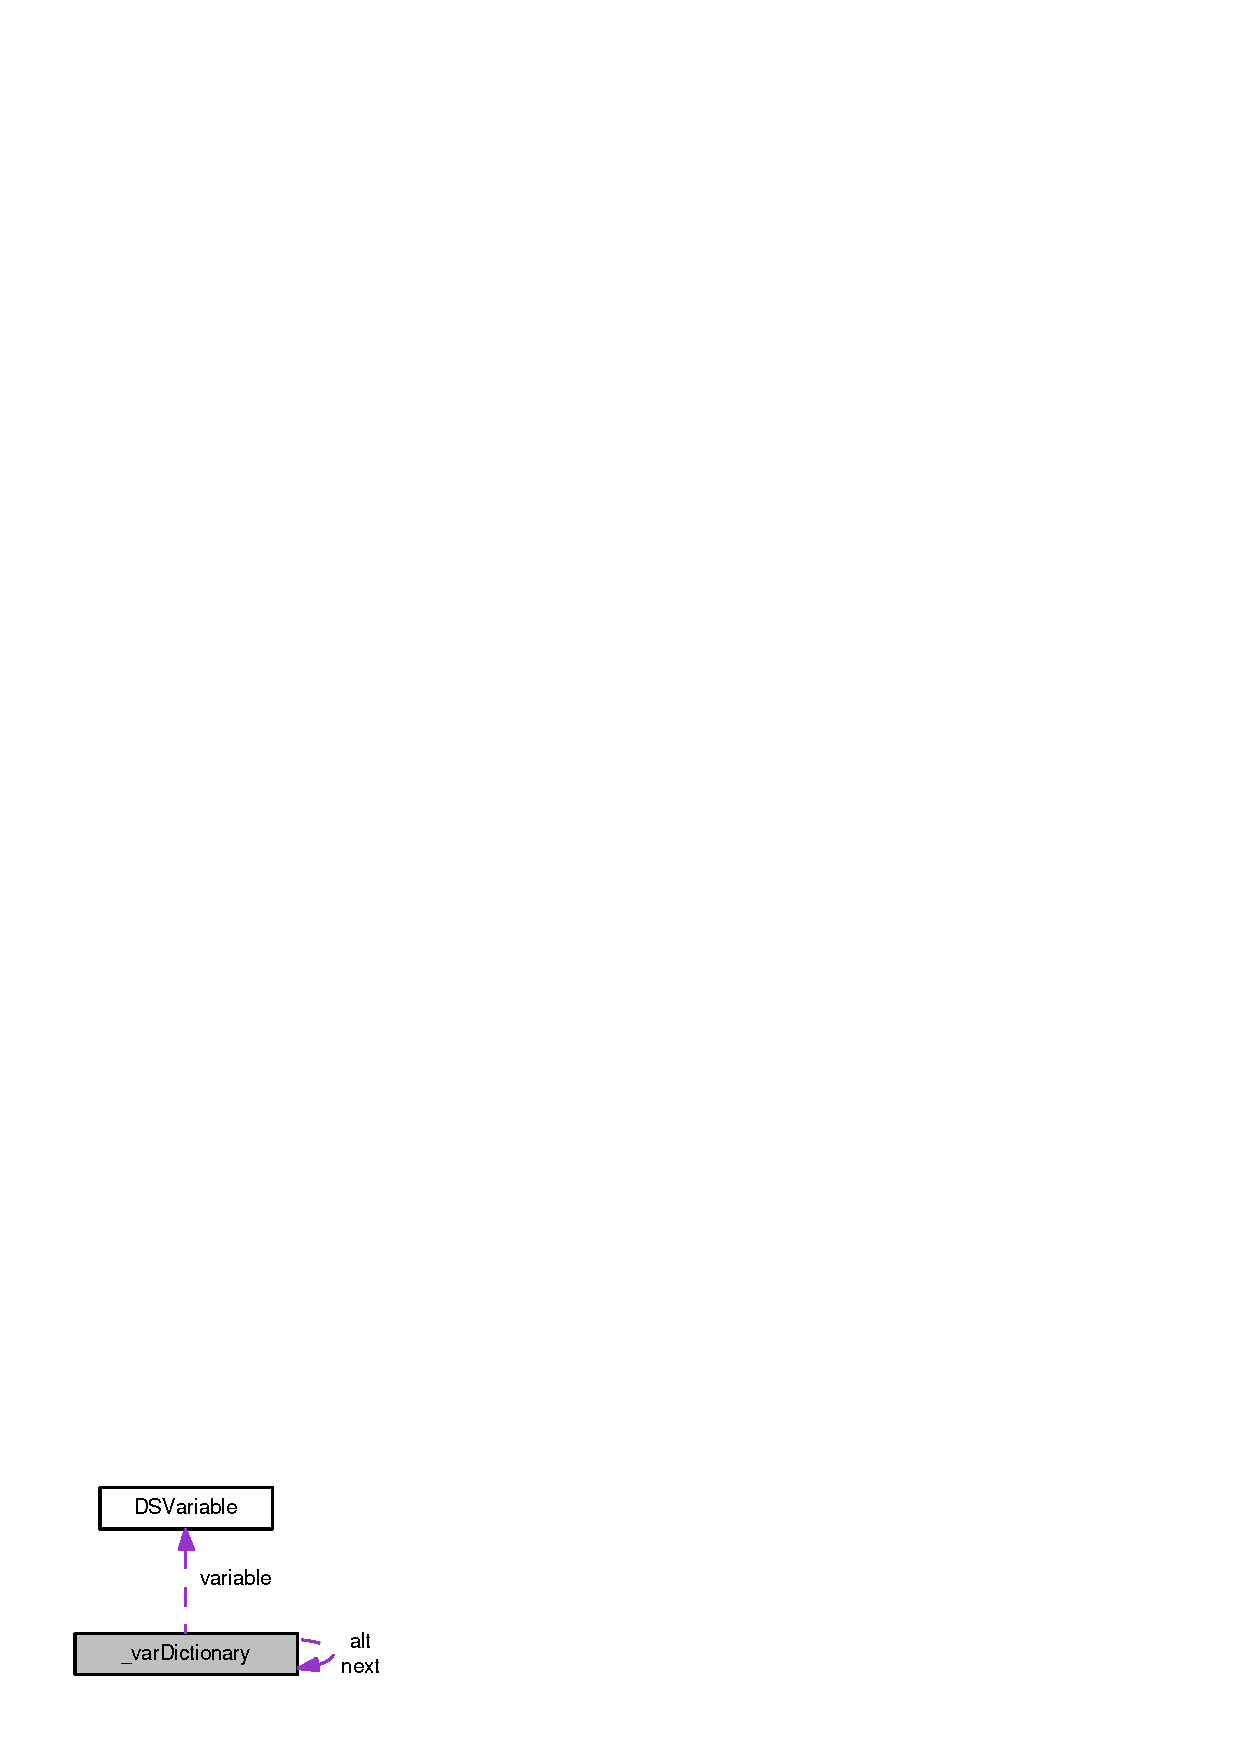
\includegraphics[width=188pt]{struct__var_dictionary__coll__graph}
\end{center}
\end{figure}
\subsection*{Data Fields}
\begin{DoxyCompactItemize}
\item 
\hypertarget{struct__var_dictionary_a6044b553e445970269cef9b91569d09d}{
char \hyperlink{struct__var_dictionary_a6044b553e445970269cef9b91569d09d}{current}}
\label{struct__var_dictionary_a6044b553e445970269cef9b91569d09d}

\begin{DoxyCompactList}\small\item\em The current character in the dictionary. \item\end{DoxyCompactList}\item 
\hypertarget{struct__var_dictionary_a916375645732b28192e23ad0745d00ca}{
struct \hyperlink{struct__var_dictionary}{\_\-varDictionary} $\ast$ \hyperlink{struct__var_dictionary_a916375645732b28192e23ad0745d00ca}{alt}}
\label{struct__var_dictionary_a916375645732b28192e23ad0745d00ca}

\begin{DoxyCompactList}\small\item\em The alternative character in the dictionary. \item\end{DoxyCompactList}\item 
\hypertarget{struct__var_dictionary_a3fab7f59fc3c8c7babba590499c69f63}{
struct \hyperlink{struct__var_dictionary}{\_\-varDictionary} $\ast$ \hyperlink{struct__var_dictionary_a3fab7f59fc3c8c7babba590499c69f63}{next}}
\label{struct__var_dictionary_a3fab7f59fc3c8c7babba590499c69f63}

\begin{DoxyCompactList}\small\item\em The next character in the dictionary. \item\end{DoxyCompactList}\item 
\hypertarget{struct__var_dictionary_a09be400084754591a8f182e4a2c83304}{
\hyperlink{struct_d_s_variable}{DSVariable} $\ast$ \hyperlink{struct__var_dictionary_a09be400084754591a8f182e4a2c83304}{variable}}
\label{struct__var_dictionary_a09be400084754591a8f182e4a2c83304}

\begin{DoxyCompactList}\small\item\em The variable stored. Only when current is '$\backslash$0'. \item\end{DoxyCompactList}\end{DoxyCompactItemize}


\subsection{Detailed Description}
Internal dictionary structure. Internal dictionary for fast variable querying. The structure of the dictionary uses an alternative path, where each character is checked in order at each position, if there is a match, the next position is consequently checked. The dictionary should never be manipulated manually, adding, retrieving and removing variables should be done through the accesory functions.

\begin{DoxySeeAlso}{See also}
\hyperlink{struct_d_s_variable}{DSVariable} 
\end{DoxySeeAlso}


The documentation for this struct was generated from the following file:\begin{DoxyCompactItemize}
\item 
\hyperlink{_d_s_types_8h}{DSTypes.h}\end{DoxyCompactItemize}

\hypertarget{unionparser__aux_1_1base__info}{
\section{base\_\-info Union Reference}
\label{unionparser__aux_1_1base__info}\index{parser\_\-aux::base\_\-info@{parser\_\-aux::base\_\-info}}
}
\subsection*{Data Fields}
\begin{DoxyCompactItemize}
\item 
\hypertarget{unionparser__aux_1_1base__info_a5ac083a645d964373f022d03df4849c8}{
char $\ast$ \hyperlink{unionparser__aux_1_1base__info_a5ac083a645d964373f022d03df4849c8}{name}}
\label{unionparser__aux_1_1base__info_a5ac083a645d964373f022d03df4849c8}

\begin{DoxyCompactList}\small\item\em The string representing the name of the variable. \item\end{DoxyCompactList}\item 
\hypertarget{unionparser__aux_1_1base__info_aee90379adb0307effb138f4871edbc5c}{
double \hyperlink{unionparser__aux_1_1base__info_aee90379adb0307effb138f4871edbc5c}{value}}
\label{unionparser__aux_1_1base__info_aee90379adb0307effb138f4871edbc5c}

\begin{DoxyCompactList}\small\item\em The variable representing the value of a constant. \item\end{DoxyCompactList}\end{DoxyCompactItemize}


The documentation for this union was generated from the following file:\begin{DoxyCompactItemize}
\item 
\hyperlink{_d_s_g_m_a_system_parsing_aux_8h}{DSGMASystemParsingAux.h}\end{DoxyCompactItemize}

\hypertarget{structds__parallelstack__t}{
\section{ds\_\-parallelstack\_\-t Struct Reference}
\label{structds__parallelstack__t}\index{ds\_\-parallelstack\_\-t@{ds\_\-parallelstack\_\-t}}
}


Stack object used by the worker threads.  




{\ttfamily \#include $<$DSDesignSpaceParallel.h$>$}



Collaboration diagram for ds\_\-parallelstack\_\-t:\subsection*{Data Fields}
\begin{DoxyCompactItemize}
\item 
\hypertarget{structds__parallelstack__t_a8add4d29bc25bbbee2f804a4d9707d40}{
DSUInteger $\ast$ \hyperlink{structds__parallelstack__t_a8add4d29bc25bbbee2f804a4d9707d40}{base}}
\label{structds__parallelstack__t_a8add4d29bc25bbbee2f804a4d9707d40}

\begin{DoxyCompactList}\small\item\em The pointer to the array of DSUIntegers storing the case numbers. \item\end{DoxyCompactList}\item 
\hypertarget{structds__parallelstack__t_aff609a2b2facf914d571229fd71fbfa6}{
DSUInteger $\ast$ \hyperlink{structds__parallelstack__t_aff609a2b2facf914d571229fd71fbfa6}{current}}
\label{structds__parallelstack__t_aff609a2b2facf914d571229fd71fbfa6}

\begin{DoxyCompactList}\small\item\em A pointer to the top of the stack. \item\end{DoxyCompactList}\item 
\hypertarget{structds__parallelstack__t_a6e9cf56a395f2344f3c8b59e09d6ae69}{
DSUInteger \hyperlink{structds__parallelstack__t_a6e9cf56a395f2344f3c8b59e09d6ae69}{count}}
\label{structds__parallelstack__t_a6e9cf56a395f2344f3c8b59e09d6ae69}

\begin{DoxyCompactList}\small\item\em The number of elements in the stack. \item\end{DoxyCompactList}\item 
\hypertarget{structds__parallelstack__t_ad8fde692241cfe9be893d63d9cc061a6}{
DSUInteger \hyperlink{structds__parallelstack__t_ad8fde692241cfe9be893d63d9cc061a6}{size}}
\label{structds__parallelstack__t_ad8fde692241cfe9be893d63d9cc061a6}

\begin{DoxyCompactList}\small\item\em The current size of the base array. \item\end{DoxyCompactList}\item 
\hypertarget{structds__parallelstack__t_aae101357fa322c8d155dd03b50a7a13b}{
DSUInteger \hyperlink{structds__parallelstack__t_aae101357fa322c8d155dd03b50a7a13b}{nextIndex}}
\label{structds__parallelstack__t_aae101357fa322c8d155dd03b50a7a13b}

\begin{DoxyCompactList}\small\item\em The index of the current case. \item\end{DoxyCompactList}\item 
\hypertarget{structds__parallelstack__t_afa7b439dc6ec7721726441e704fe6493}{
\hyperlink{struct_d_s_case}{DSCase} $\ast$$\ast$ \hyperlink{structds__parallelstack__t_afa7b439dc6ec7721726441e704fe6493}{cases}}
\label{structds__parallelstack__t_afa7b439dc6ec7721726441e704fe6493}

\begin{DoxyCompactList}\small\item\em The array of cases processed. \item\end{DoxyCompactList}\item 
\hypertarget{structds__parallelstack__t_a7710776f2028c036203f5b6f77686749}{
pthread\_\-mutex\_\-t \hyperlink{structds__parallelstack__t_a7710776f2028c036203f5b6f77686749}{pushpop}}
\label{structds__parallelstack__t_a7710776f2028c036203f5b6f77686749}

\begin{DoxyCompactList}\small\item\em The mutex used when pushing and popping data from the stack. \item\end{DoxyCompactList}\end{DoxyCompactItemize}


\subsection{Detailed Description}
Stack object used by the worker threads. This structure is a stack of case numbers indicating the DSCases that need to be processed, and each pthread\_\-t used for processing cases and determining validity (currently disabled due to the non re-\/entrant GLPK) must have access to a \hyperlink{structds__parallelstack__t}{ds\_\-parallelstack\_\-t}.

\begin{DoxyNote}{Note}
One stack should be created per thread, to avoid one thread blocking another during popping and pushing operations. A single stack could be used, as the parallel stacks are thread safe, and under some conditions might be more efficient as all the threads in the thread pool will remain active until all cases have been processed. Currently, the number of cases to be processed by a thread are determined prior to launching the threads, and each thread has an equal number of cases to process. If a thread has many invalid cases, it may finish all of its cases before the other threads, and thus it is possible for the system to make less use of multiple processors. To avoid this situation, more threads than processors can be used or a single shared stack could be used. 
\end{DoxyNote}


The documentation for this struct was generated from the following file:\begin{DoxyCompactItemize}
\item 
\hyperlink{_d_s_design_space_parallel_8h}{DSDesignSpaceParallel.h}\end{DoxyCompactItemize}

\hypertarget{struct_d_s_case}{
\section{DSCase Struct Reference}
\label{struct_d_s_case}\index{DSCase@{DSCase}}
}


Data type used to represent a case.  




{\ttfamily \#include $<$DSTypes.h$>$}



Collaboration diagram for DSCase:\subsection*{Data Fields}
\begin{DoxyCompactItemize}
\item 
\hypertarget{struct_d_s_case_a739550585a18a79b3f809fc0b0d2658b}{
const \hyperlink{struct_d_s_variable_pool}{DSVariablePool} $\ast$ \hyperlink{struct_d_s_case_a739550585a18a79b3f809fc0b0d2658b}{Xd}}
\label{struct_d_s_case_a739550585a18a79b3f809fc0b0d2658b}

\begin{DoxyCompactList}\small\item\em A pointer to the \hyperlink{struct_d_s_variable_pool}{DSVariablePool} with the dependent variables. \item\end{DoxyCompactList}\item 
\hypertarget{struct_d_s_case_a00cfed7027afc5b8218687b951287742}{
const \hyperlink{struct_d_s_variable_pool}{DSVariablePool} $\ast$ \hyperlink{struct_d_s_case_a00cfed7027afc5b8218687b951287742}{Xi}}
\label{struct_d_s_case_a00cfed7027afc5b8218687b951287742}

\begin{DoxyCompactList}\small\item\em A pointer to the \hyperlink{struct_d_s_variable_pool}{DSVariablePool} with the independent variables. \item\end{DoxyCompactList}\item 
\hypertarget{struct_d_s_case_abb70d0151846760d948b6197579c4311}{
\hyperlink{struct_d_s_s_system}{DSSSystem} $\ast$ \hyperlink{struct_d_s_case_abb70d0151846760d948b6197579c4311}{ssys}}
\label{struct_d_s_case_abb70d0151846760d948b6197579c4311}

\begin{DoxyCompactList}\small\item\em The \hyperlink{struct_d_s_s_system}{DSSSystem} of the case. \item\end{DoxyCompactList}\item 
\hypertarget{struct_d_s_case_a3f0ef631e7fc4b26d38a5ddb6555cf99}{
\hyperlink{struct_d_s_matrix}{DSMatrix} $\ast$ \hyperlink{struct_d_s_case_a3f0ef631e7fc4b26d38a5ddb6555cf99}{Cd}}
\label{struct_d_s_case_a3f0ef631e7fc4b26d38a5ddb6555cf99}

\begin{DoxyCompactList}\small\item\em The condition matrix corresponding to the dependent variables. \item\end{DoxyCompactList}\item 
\hypertarget{struct_d_s_case_a15a8ddd0ce51e986b28e6bd347a03c4e}{
\hyperlink{struct_d_s_matrix}{DSMatrix} $\ast$ \hyperlink{struct_d_s_case_a15a8ddd0ce51e986b28e6bd347a03c4e}{Ci}}
\label{struct_d_s_case_a15a8ddd0ce51e986b28e6bd347a03c4e}

\begin{DoxyCompactList}\small\item\em The condition matrix corresponding to the independent variables. \item\end{DoxyCompactList}\item 
\hypertarget{struct_d_s_case_a2414d45c3be60e7ce067340f628bca3a}{
\hyperlink{struct_d_s_matrix}{DSMatrix} $\ast$ \hyperlink{struct_d_s_case_a2414d45c3be60e7ce067340f628bca3a}{U}}
\label{struct_d_s_case_a2414d45c3be60e7ce067340f628bca3a}

\begin{DoxyCompactList}\small\item\em The boundary matrix corresponding to the independent variables. \item\end{DoxyCompactList}\item 
\hypertarget{struct_d_s_case_add8d5891b05771aadcaf8c02b8b3eaec}{
\hyperlink{struct_d_s_matrix}{DSMatrix} $\ast$ \hyperlink{struct_d_s_case_add8d5891b05771aadcaf8c02b8b3eaec}{delta}}
\label{struct_d_s_case_add8d5891b05771aadcaf8c02b8b3eaec}

\begin{DoxyCompactList}\small\item\em The condition matrix corresponding to the constants. \item\end{DoxyCompactList}\item 
\hypertarget{struct_d_s_case_aa4b266ea97ab90471cced4315c114e44}{
\hyperlink{struct_d_s_matrix}{DSMatrix} $\ast$ \hyperlink{struct_d_s_case_aa4b266ea97ab90471cced4315c114e44}{zeta}}
\label{struct_d_s_case_aa4b266ea97ab90471cced4315c114e44}

\begin{DoxyCompactList}\small\item\em The boundary matrix corresponding to the constants. \item\end{DoxyCompactList}\item 
\hypertarget{struct_d_s_case_a6cd3e79aa8ec931d4d3bad3723606efe}{
DSUInteger \hyperlink{struct_d_s_case_a6cd3e79aa8ec931d4d3bad3723606efe}{caseNumber}}
\label{struct_d_s_case_a6cd3e79aa8ec931d4d3bad3723606efe}

\begin{DoxyCompactList}\small\item\em The case number used to identify the case. \item\end{DoxyCompactList}\item 
\hypertarget{struct_d_s_case_a2bfb90f4fc55714f8fd9b9dfbfd21e32}{
DSUInteger $\ast$ \hyperlink{struct_d_s_case_a2bfb90f4fc55714f8fd9b9dfbfd21e32}{signature}}
\label{struct_d_s_case_a2bfb90f4fc55714f8fd9b9dfbfd21e32}

\begin{DoxyCompactList}\small\item\em The case signature indicating the dominant terms used to generate the case. \item\end{DoxyCompactList}\end{DoxyCompactItemize}


\subsection{Detailed Description}
Data type used to represent a case. This data type has all the necessary information for a case in design space. It has a pointer to the dependent and independent variables of the system, a pointer to the corresponding S-\/System, the Condition matrices and boundary matrices. It also has information about the case number and case signature.

\begin{DoxyNote}{Note}
The case number is arbitrary, and can be generated by two algorithms to be either big endian or small endian. For compatibility with the current design space toolbox, big endian is the default.

The case is not responsible for freeing the Xd and Xi data structures. If the case is generated from a design space, then the design space is responsible for freeing the Xi and Xd variable pools; otherwise the internal S-\/System is responsible for freeing this data. 
\end{DoxyNote}


The documentation for this struct was generated from the following file:\begin{DoxyCompactItemize}
\item 
\hyperlink{_d_s_types_8h}{DSTypes.h}\end{DoxyCompactItemize}

\hypertarget{struct_d_s_design_space}{
\section{DSDesignSpace Struct Reference}
\label{struct_d_s_design_space}\index{DSDesignSpace@{DSDesignSpace}}
}


Data type used to represent a design space.  




{\ttfamily \#include $<$DSTypes.h$>$}



Collaboration diagram for DSDesignSpace:\subsection*{Data Fields}
\begin{DoxyCompactItemize}
\item 
\hypertarget{struct_d_s_design_space_ace45d99580d7db1513538aeb7678b6db}{
\hyperlink{struct_d_s_g_m_a_system}{DSGMASystem} $\ast$ \hyperlink{struct_d_s_design_space_ace45d99580d7db1513538aeb7678b6db}{gma}}
\label{struct_d_s_design_space_ace45d99580d7db1513538aeb7678b6db}

\begin{DoxyCompactList}\small\item\em The gma system of the design space. \item\end{DoxyCompactList}\item 
\hypertarget{struct_d_s_design_space_a739550585a18a79b3f809fc0b0d2658b}{
const \hyperlink{struct_d_s_variable_pool}{DSVariablePool} $\ast$ \hyperlink{struct_d_s_design_space_a739550585a18a79b3f809fc0b0d2658b}{Xd}}
\label{struct_d_s_design_space_a739550585a18a79b3f809fc0b0d2658b}

\begin{DoxyCompactList}\small\item\em A pointer to the \hyperlink{struct_d_s_variable_pool}{DSVariablePool} with the dependent variables. \item\end{DoxyCompactList}\item 
\hypertarget{struct_d_s_design_space_a00cfed7027afc5b8218687b951287742}{
const \hyperlink{struct_d_s_variable_pool}{DSVariablePool} $\ast$ \hyperlink{struct_d_s_design_space_a00cfed7027afc5b8218687b951287742}{Xi}}
\label{struct_d_s_design_space_a00cfed7027afc5b8218687b951287742}

\begin{DoxyCompactList}\small\item\em A pointer to the \hyperlink{struct_d_s_variable_pool}{DSVariablePool} with the dependent variables. \item\end{DoxyCompactList}\item 
\hypertarget{struct_d_s_design_space_ac9ccac5ae8d5a9b6255b2bb394d90b53}{
\hyperlink{struct_d_s_dictionary}{DSDictionary} $\ast$ \hyperlink{struct_d_s_design_space_ac9ccac5ae8d5a9b6255b2bb394d90b53}{validCases}}
\label{struct_d_s_design_space_ac9ccac5ae8d5a9b6255b2bb394d90b53}

\begin{DoxyCompactList}\small\item\em \hyperlink{struct_d_s_variable_pool}{DSVariablePool} with case number that are valid. \item\end{DoxyCompactList}\item 
\hypertarget{struct_d_s_design_space_a13b1ed4c5a74f8af8c169edc3a04d41a}{
DSUInteger \hyperlink{struct_d_s_design_space_a13b1ed4c5a74f8af8c169edc3a04d41a}{numberOfCases}}
\label{struct_d_s_design_space_a13b1ed4c5a74f8af8c169edc3a04d41a}

\begin{DoxyCompactList}\small\item\em DSUInteger indicating the maximum number of cases in the design space. \item\end{DoxyCompactList}\item 
\hypertarget{struct_d_s_design_space_a3f0ef631e7fc4b26d38a5ddb6555cf99}{
\hyperlink{struct_d_s_matrix}{DSMatrix} $\ast$ {\bfseries Cd}}
\label{struct_d_s_design_space_a3f0ef631e7fc4b26d38a5ddb6555cf99}

\item 
\hypertarget{struct_d_s_design_space_abc83f4bb21d43d8bc1f6228d3c66853e}{
\hyperlink{struct_d_s_matrix}{DSMatrix} $\ast$ {\bfseries Ci}}
\label{struct_d_s_design_space_abc83f4bb21d43d8bc1f6228d3c66853e}

\item 
\hypertarget{struct_d_s_design_space_a565e0140e786d762f8a608dcc2e227ef}{
\hyperlink{struct_d_s_matrix}{DSMatrix} $\ast$ \hyperlink{struct_d_s_design_space_a565e0140e786d762f8a608dcc2e227ef}{delta}}
\label{struct_d_s_design_space_a565e0140e786d762f8a608dcc2e227ef}

\begin{DoxyCompactList}\small\item\em Condition matrices. \item\end{DoxyCompactList}\item 
\hypertarget{struct_d_s_design_space_a246cb0cf43ca5193adfd233273c34009}{
\hyperlink{struct_d_s_dictionary}{DSDictionary} $\ast$ \hyperlink{struct_d_s_design_space_a246cb0cf43ca5193adfd233273c34009}{subcases}}
\label{struct_d_s_design_space_a246cb0cf43ca5193adfd233273c34009}

\begin{DoxyCompactList}\small\item\em DSDesignSpaceStack containing design space objects with subcases. \item\end{DoxyCompactList}\end{DoxyCompactItemize}


\subsection{Detailed Description}
Data type used to represent a design space. The design space data structure is a convenience structure that automates the construction and analysis of cases, and manages the memory associated with these cases. This behavior can be avoided by working directly with the gma system of the designspace.

\begin{DoxySeeAlso}{See also}
\hyperlink{_d_s_design_space_8h}{DSDesignSpace.h} 

\hyperlink{_d_s_design_space_8c}{DSDesignSpace.c} 
\end{DoxySeeAlso}


The documentation for this struct was generated from the following file:\begin{DoxyCompactItemize}
\item 
\hyperlink{_d_s_types_8h}{DSTypes.h}\end{DoxyCompactItemize}

\hypertarget{struct_d_s_design_space_stack}{
\section{DSDesignSpaceStack Struct Reference}
\label{struct_d_s_design_space_stack}\index{DSDesignSpaceStack@{DSDesignSpaceStack}}
}
\subsection*{Data Fields}
\begin{DoxyCompactItemize}
\item 
\hypertarget{struct_d_s_design_space_stack_a16826c910c478e10e6058011089c3318}{
DSUInteger $\ast$ {\bfseries caseNumber}}
\label{struct_d_s_design_space_stack_a16826c910c478e10e6058011089c3318}

\item 
\hypertarget{struct_d_s_design_space_stack_a21ae974807506e3b4e1b7d5703ee3d16}{
DSUInteger $\ast$ {\bfseries caseNumberCurrent}}
\label{struct_d_s_design_space_stack_a21ae974807506e3b4e1b7d5703ee3d16}

\item 
\hypertarget{struct_d_s_design_space_stack_a249441016c880f0801b380bd22cedcc6}{
void $\ast$$\ast$ \hyperlink{struct_d_s_design_space_stack_a249441016c880f0801b380bd22cedcc6}{base}}
\label{struct_d_s_design_space_stack_a249441016c880f0801b380bd22cedcc6}

\begin{DoxyCompactList}\small\item\em The pointer to the array of DSUIntegers storing the case numbers. \item\end{DoxyCompactList}\item 
\hypertarget{struct_d_s_design_space_stack_ab6c47e43f38d68ed97c3f6c7973d1444}{
void $\ast$$\ast$ \hyperlink{struct_d_s_design_space_stack_ab6c47e43f38d68ed97c3f6c7973d1444}{current}}
\label{struct_d_s_design_space_stack_ab6c47e43f38d68ed97c3f6c7973d1444}

\begin{DoxyCompactList}\small\item\em A pointer to the top of the stack. \item\end{DoxyCompactList}\item 
\hypertarget{struct_d_s_design_space_stack_a6e9cf56a395f2344f3c8b59e09d6ae69}{
DSUInteger \hyperlink{struct_d_s_design_space_stack_a6e9cf56a395f2344f3c8b59e09d6ae69}{count}}
\label{struct_d_s_design_space_stack_a6e9cf56a395f2344f3c8b59e09d6ae69}

\begin{DoxyCompactList}\small\item\em The number of elements in the stack. \item\end{DoxyCompactList}\item 
\hypertarget{struct_d_s_design_space_stack_ad8fde692241cfe9be893d63d9cc061a6}{
DSUInteger \hyperlink{struct_d_s_design_space_stack_ad8fde692241cfe9be893d63d9cc061a6}{size}}
\label{struct_d_s_design_space_stack_ad8fde692241cfe9be893d63d9cc061a6}

\begin{DoxyCompactList}\small\item\em The current size of the base array. \item\end{DoxyCompactList}\item 
\hypertarget{struct_d_s_design_space_stack_a7710776f2028c036203f5b6f77686749}{
pthread\_\-mutex\_\-t \hyperlink{struct_d_s_design_space_stack_a7710776f2028c036203f5b6f77686749}{pushpop}}
\label{struct_d_s_design_space_stack_a7710776f2028c036203f5b6f77686749}

\begin{DoxyCompactList}\small\item\em The mutex used when pushing and popping data from the stack. \item\end{DoxyCompactList}\end{DoxyCompactItemize}


The documentation for this struct was generated from the following file:\begin{DoxyCompactItemize}
\item 
\hyperlink{_d_s_types_8h}{DSTypes.h}\end{DoxyCompactItemize}

\hypertarget{structdsexpression}{
\section{dsexpression Struct Reference}
\label{structdsexpression}\index{dsexpression@{dsexpression}}
}


Data type representing mathematical expressions.  




{\ttfamily \#include $<$DSTypes.h$>$}



Collaboration diagram for dsexpression:\subsection*{Data Fields}
\begin{DoxyCompactItemize}
\item 
\hypertarget{structdsexpression_ac18b7c5a93ab2669c0060bda434e3954}{
\begin{tabbing}
xx\=xx\=xx\=xx\=xx\=xx\=xx\=xx\=xx\=\kill
union \{\\
\>char {\bfseries op\_code}\\
\>double {\bfseries constant}\\
\>char $\ast$ \hyperlink{structdsexpression_aab7679056ef1a7836a49d5a2eab18a8f}{variable}\\
\>\>{\em A string with the name of the variable. }\\
\} \hyperlink{structdsexpression_ac18b7c5a93ab2669c0060bda434e3954}{node}}
\label{structdsexpression_ac18b7c5a93ab2669c0060bda434e3954}
\\

\end{tabbing}\begin{DoxyCompactList}\small\item\em Union of data types potentially contained in the node. \item\end{DoxyCompactList}\item 
\hypertarget{structdsexpression_ac765329451135abec74c45e1897abf26}{
int \hyperlink{structdsexpression_ac765329451135abec74c45e1897abf26}{type}}
\label{structdsexpression_ac765329451135abec74c45e1897abf26}

\begin{DoxyCompactList}\small\item\em Integer specifying the type of node. \item\end{DoxyCompactList}\item 
\hypertarget{structdsexpression_abef8ea275a9a4e96c207d06a5b409d4a}{
int \hyperlink{structdsexpression_abef8ea275a9a4e96c207d06a5b409d4a}{numberOfBranches}}
\label{structdsexpression_abef8ea275a9a4e96c207d06a5b409d4a}

\begin{DoxyCompactList}\small\item\em Number of branches of children, relevant to operators and functions. \item\end{DoxyCompactList}\item 
\hypertarget{structdsexpression_a35237107e14601d760b6bcd9cc0af0e2}{
struct \hyperlink{structdsexpression}{dsexpression} $\ast$$\ast$ \hyperlink{structdsexpression_a35237107e14601d760b6bcd9cc0af0e2}{branches}}
\label{structdsexpression_a35237107e14601d760b6bcd9cc0af0e2}

\begin{DoxyCompactList}\small\item\em Array of expression nodes with children nodes. \item\end{DoxyCompactList}\end{DoxyCompactItemize}


\subsection{Detailed Description}
Data type representing mathematical expressions. This data type is the internal representation of matematical expressions. This data type is an Abstracts Syntax Tree with only three operators: '+', '$\ast$' and '$^\wedge$'. All other operators ('-\/' and '/') are represented by a combination of the former operators. The DSExpression automatically groups constant values, and reserves the first branch of the multiplication and addition operator for constant values. These operators can have any number of branches. The '$^\wedge$' operator can have two, and only two, branches.

\begin{DoxyNote}{Note}
Functions are handled as variables with a single argument
\end{DoxyNote}
\begin{DoxySeeAlso}{See also}
\hyperlink{_d_s_expression_8h}{DSExpression.h} 

\hyperlink{_d_s_expression_8c}{DSExpression.c} 
\end{DoxySeeAlso}


The documentation for this struct was generated from the following file:\begin{DoxyCompactItemize}
\item 
\hyperlink{_d_s_types_8h}{DSTypes.h}\end{DoxyCompactItemize}

\hypertarget{struct_d_s_g_m_a_system}{
\section{DSGMASystem Struct Reference}
\label{struct_d_s_g_m_a_system}\index{DSGMASystem@{DSGMASystem}}
}


Data type representing a GMA-\/System.  




{\ttfamily \#include $<$DSTypes.h$>$}



Collaboration diagram for DSGMASystem:\subsection*{Data Fields}
\begin{DoxyCompactItemize}
\item 
\hypertarget{struct_d_s_g_m_a_system_af359cac84c0852ea6846009021b61da3}{
char $\ast$$\ast$ {\bfseries equations}}
\label{struct_d_s_g_m_a_system_af359cac84c0852ea6846009021b61da3}

\item 
\hypertarget{struct_d_s_g_m_a_system_a3d42a9503ac28b35558ac1138c0bd0fc}{
\hyperlink{struct_d_s_matrix}{DSMatrix} $\ast$ {\bfseries alpha}}
\label{struct_d_s_g_m_a_system_a3d42a9503ac28b35558ac1138c0bd0fc}

\item 
\hypertarget{struct_d_s_g_m_a_system_a1bb699dd7e2b8dadbb12f86cb9697004}{
\hyperlink{struct_d_s_matrix}{DSMatrix} $\ast$ {\bfseries beta}}
\label{struct_d_s_g_m_a_system_a1bb699dd7e2b8dadbb12f86cb9697004}

\item 
\hypertarget{struct_d_s_g_m_a_system_acdf77ac56f2229762c650415d1fc53ed}{
\hyperlink{struct_d_s_matrix_array}{DSMatrixArray} $\ast$ {\bfseries Gd}}
\label{struct_d_s_g_m_a_system_acdf77ac56f2229762c650415d1fc53ed}

\item 
\hypertarget{struct_d_s_g_m_a_system_aab7953fe5487c282f8ab07f3c7a55257}{
\hyperlink{struct_d_s_matrix_array}{DSMatrixArray} $\ast$ {\bfseries Gi}}
\label{struct_d_s_g_m_a_system_aab7953fe5487c282f8ab07f3c7a55257}

\item 
\hypertarget{struct_d_s_g_m_a_system_a512e6ff827f3a69d68e5f3400e02a55f}{
\hyperlink{struct_d_s_matrix_array}{DSMatrixArray} $\ast$ {\bfseries Hd}}
\label{struct_d_s_g_m_a_system_a512e6ff827f3a69d68e5f3400e02a55f}

\item 
\hypertarget{struct_d_s_g_m_a_system_a7a3ca05ca1b7aeecf830a58fe217cac8}{
\hyperlink{struct_d_s_matrix_array}{DSMatrixArray} $\ast$ {\bfseries Hi}}
\label{struct_d_s_g_m_a_system_a7a3ca05ca1b7aeecf830a58fe217cac8}

\item 
\hypertarget{struct_d_s_g_m_a_system_a2827047336233c327d6eeb0564d3b3aa}{
\hyperlink{struct_d_s_variable_pool}{DSVariablePool} $\ast$ {\bfseries Xd}}
\label{struct_d_s_g_m_a_system_a2827047336233c327d6eeb0564d3b3aa}

\item 
\hypertarget{struct_d_s_g_m_a_system_a0f2d639685f52fa1a385a8ceaff90686}{
\hyperlink{struct_d_s_variable_pool}{DSVariablePool} $\ast$ {\bfseries Xi}}
\label{struct_d_s_g_m_a_system_a0f2d639685f52fa1a385a8ceaff90686}

\item 
\hypertarget{struct_d_s_g_m_a_system_a2bfb90f4fc55714f8fd9b9dfbfd21e32}{
DSUInteger $\ast$ {\bfseries signature}}
\label{struct_d_s_g_m_a_system_a2bfb90f4fc55714f8fd9b9dfbfd21e32}

\end{DoxyCompactItemize}


\subsection{Detailed Description}
Data type representing a GMA-\/System. This data structure is a standard representation of an GMA using matrix notation. Here, the positive and negative terms are explicitly represented according to the Gs and Hs. Also, matrices are split up relating to either dependent and independent parameters. The GMA system uses an array of matrices to represent all the terms in all of the equations. 

The documentation for this struct was generated from the following file:\begin{DoxyCompactItemize}
\item 
\hyperlink{_d_s_types_8h}{DSTypes.h}\end{DoxyCompactItemize}

\hypertarget{struct_d_s_matrix}{
\section{DSMatrix Struct Reference}
\label{struct_d_s_matrix}\index{DSMatrix@{DSMatrix}}
}


Data type representing a matrix.  




{\ttfamily \#include $<$DSTypes.h$>$}

\subsection*{Data Fields}
\begin{DoxyCompactItemize}
\item 
\hypertarget{struct_d_s_matrix_a98815eee0ec0d8a86f2632f922df6e36}{
void $\ast$ \hyperlink{struct_d_s_matrix_a98815eee0ec0d8a86f2632f922df6e36}{mat}}
\label{struct_d_s_matrix_a98815eee0ec0d8a86f2632f922df6e36}

\begin{DoxyCompactList}\small\item\em The pointer to the internal representation of the matrix. \item\end{DoxyCompactList}\item 
\hypertarget{struct_d_s_matrix_abc69b7682293d99094ac37ed894a0249}{
DSUInteger \hyperlink{struct_d_s_matrix_abc69b7682293d99094ac37ed894a0249}{rows}}
\label{struct_d_s_matrix_abc69b7682293d99094ac37ed894a0249}

\begin{DoxyCompactList}\small\item\em A DSUInteger specifying the number of rows in the matrix. \item\end{DoxyCompactList}\item 
\hypertarget{struct_d_s_matrix_afb99a05f6e779cf7c631393281dddda9}{
DSUInteger \hyperlink{struct_d_s_matrix_afb99a05f6e779cf7c631393281dddda9}{columns}}
\label{struct_d_s_matrix_afb99a05f6e779cf7c631393281dddda9}

\begin{DoxyCompactList}\small\item\em A DSUInteger specifying the number of columns in the matrix. \item\end{DoxyCompactList}\end{DoxyCompactItemize}


\subsection{Detailed Description}
Data type representing a matrix. This data type is the front end of the matric manipulation portion of the design space toolbox. Currently, the DST library uses the gsl library; however, it is designed to be used with different back-\/ends. In particular, the CLAPACK package should be considered, as it will offer better performance. Thus, the matrix API should be independent of implementation, and hence a new matrix library could be used if chosen. 

The documentation for this struct was generated from the following file:\begin{DoxyCompactItemize}
\item 
\hyperlink{_d_s_types_8h}{DSTypes.h}\end{DoxyCompactItemize}

\hypertarget{struct_d_s_matrix_array}{
\section{DSMatrixArray Struct Reference}
\label{struct_d_s_matrix_array}\index{DSMatrixArray@{DSMatrixArray}}
}


Data type representing an array of matrices.  




{\ttfamily \#include $<$DSTypes.h$>$}



Collaboration diagram for DSMatrixArray:\nopagebreak
\begin{figure}[H]
\begin{center}
\leavevmode
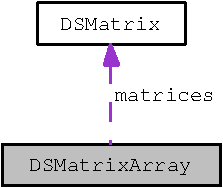
\includegraphics[width=142pt]{struct_d_s_matrix_array__coll__graph}
\end{center}
\end{figure}
\subsection*{Data Fields}
\begin{DoxyCompactItemize}
\item 
\hypertarget{struct_d_s_matrix_array_ab5f4da8dd96ac570199f6ead749797aa}{
DSUInteger \hyperlink{struct_d_s_matrix_array_ab5f4da8dd96ac570199f6ead749797aa}{numberOfMatrices}}
\label{struct_d_s_matrix_array_ab5f4da8dd96ac570199f6ead749797aa}

\begin{DoxyCompactList}\small\item\em A DSUInteger specifying the number of matrices in the array. \item\end{DoxyCompactList}\item 
\hypertarget{struct_d_s_matrix_array_a48afc9204e98afffd4acd6a5175e30f4}{
\hyperlink{struct_d_s_matrix}{DSMatrix} $\ast$$\ast$ \hyperlink{struct_d_s_matrix_array_a48afc9204e98afffd4acd6a5175e30f4}{matrices}}
\label{struct_d_s_matrix_array_a48afc9204e98afffd4acd6a5175e30f4}

\begin{DoxyCompactList}\small\item\em A pointer the the C-\/style array of matrices. \item\end{DoxyCompactList}\end{DoxyCompactItemize}


\subsection{Detailed Description}
Data type representing an array of matrices. This data type is a utility data type that keeps track of arrays of matrices. This structure is used to represent three-\/dimensional matrices, as used internally by GMA's systems.

\begin{DoxySeeAlso}{See also}
\hyperlink{_d_s_matrix_array_8h}{DSMatrixArray.h} 

\hyperlink{_d_s_matrix_array_8c}{DSMatrixArray.c} 
\end{DoxySeeAlso}


The documentation for this struct was generated from the following file:\begin{DoxyCompactItemize}
\item 
\hyperlink{_d_s_types_8h}{DSTypes.h}\end{DoxyCompactItemize}

\hypertarget{struct_d_s_s_system}{
\section{DSSSystem Struct Reference}
\label{struct_d_s_s_system}\index{DSSSystem@{DSSSystem}}
}


Data type representing an S-\/System.  




{\ttfamily \#include $<$DSTypes.h$>$}



Collaboration diagram for DSSSystem:\nopagebreak
\begin{figure}[H]
\begin{center}
\leavevmode
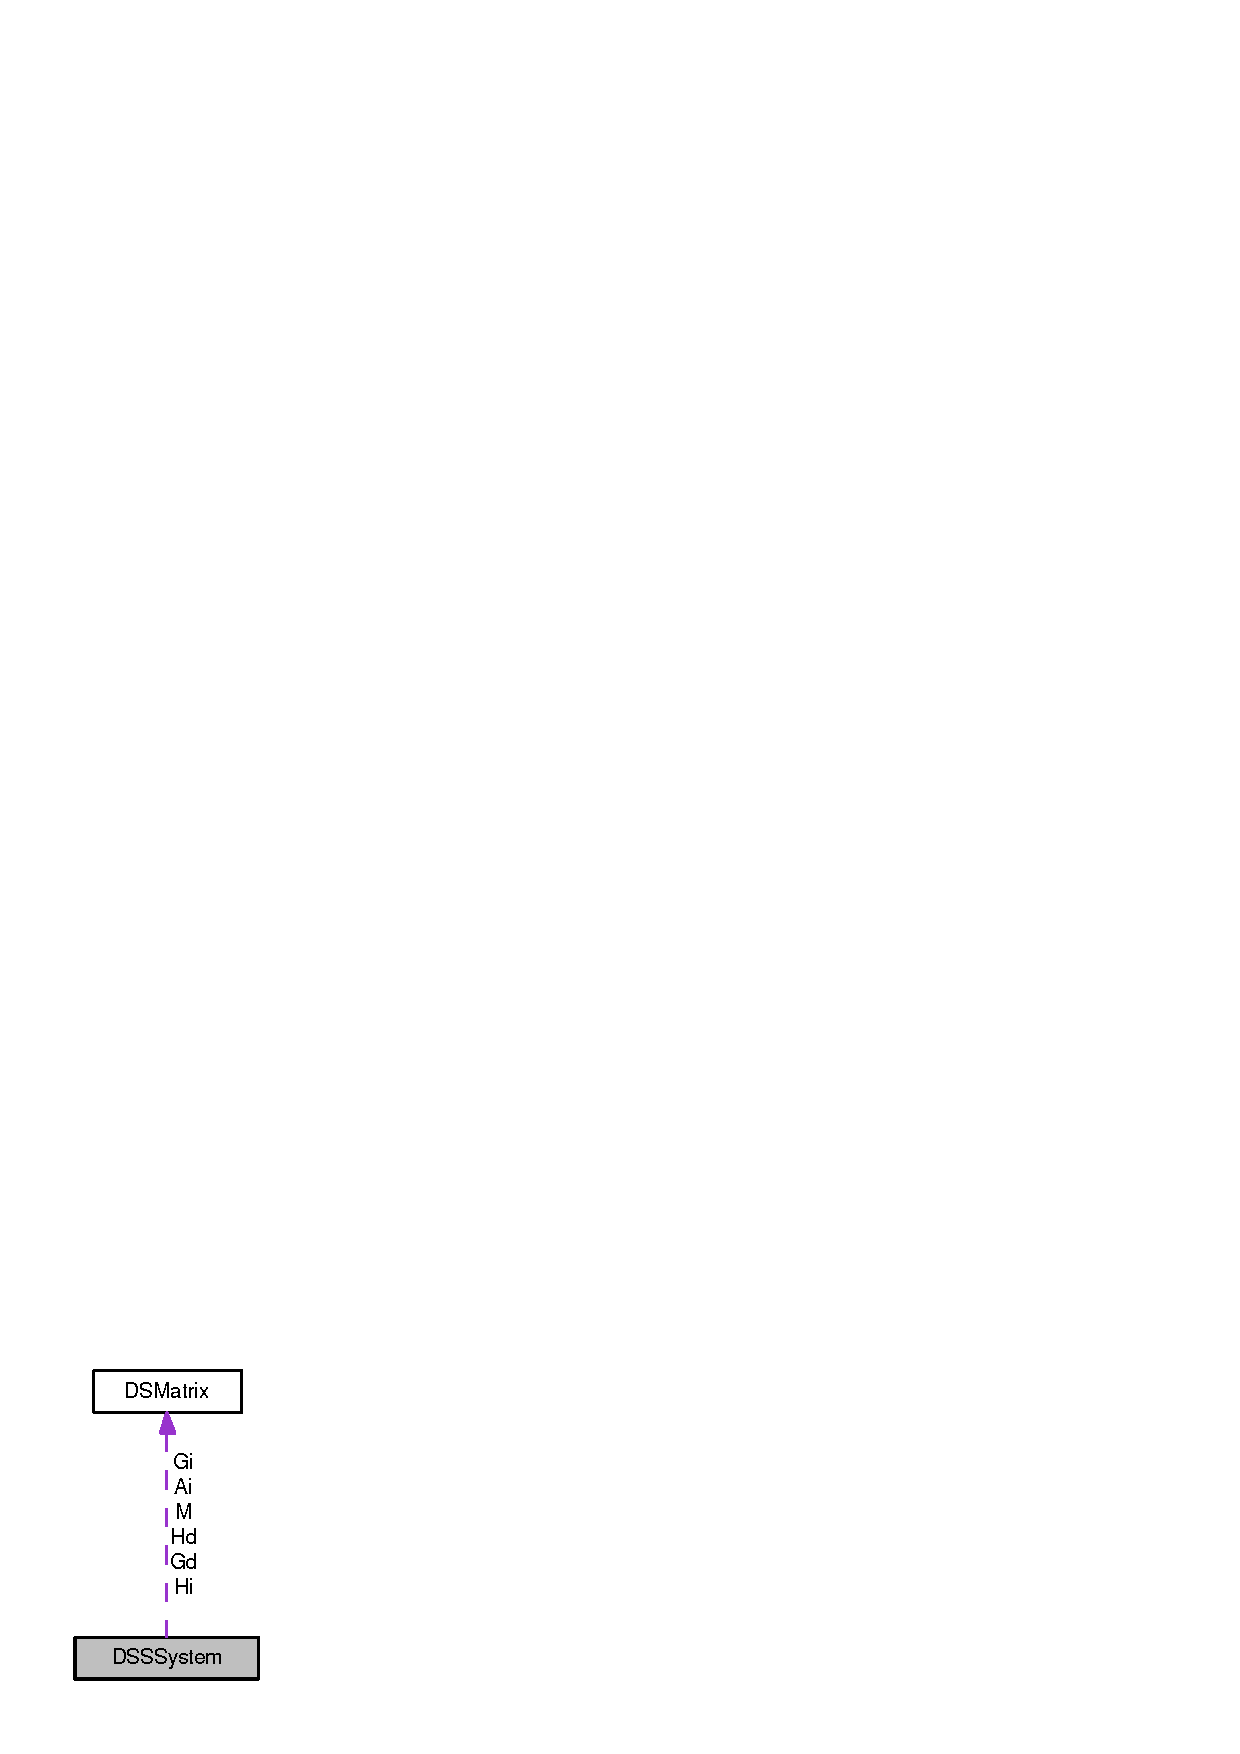
\includegraphics[width=125pt]{struct_d_s_s_system__coll__graph}
\end{center}
\end{figure}
\subsection*{Data Fields}
\begin{DoxyCompactItemize}
\item 
\hypertarget{struct_d_s_s_system_a3d42a9503ac28b35558ac1138c0bd0fc}{
\hyperlink{struct_d_s_matrix}{DSMatrix} $\ast$ {\bfseries alpha}}
\label{struct_d_s_s_system_a3d42a9503ac28b35558ac1138c0bd0fc}

\item 
\hypertarget{struct_d_s_s_system_a1bb699dd7e2b8dadbb12f86cb9697004}{
\hyperlink{struct_d_s_matrix}{DSMatrix} $\ast$ {\bfseries beta}}
\label{struct_d_s_s_system_a1bb699dd7e2b8dadbb12f86cb9697004}

\item 
\hypertarget{struct_d_s_s_system_a9b4cbb7b74e363d29d8bb9286bd2cebb}{
\hyperlink{struct_d_s_matrix}{DSMatrix} $\ast$ {\bfseries Gd}}
\label{struct_d_s_s_system_a9b4cbb7b74e363d29d8bb9286bd2cebb}

\item 
\hypertarget{struct_d_s_s_system_a75132febb300c23365aac8c8aeea7cd5}{
\hyperlink{struct_d_s_matrix}{DSMatrix} $\ast$ {\bfseries Gi}}
\label{struct_d_s_s_system_a75132febb300c23365aac8c8aeea7cd5}

\item 
\hypertarget{struct_d_s_s_system_a0ce13baa657ac43255d2b5837f50df3d}{
\hyperlink{struct_d_s_matrix}{DSMatrix} $\ast$ {\bfseries Hd}}
\label{struct_d_s_s_system_a0ce13baa657ac43255d2b5837f50df3d}

\item 
\hypertarget{struct_d_s_s_system_ab94594d92720ee99410ddf151d7757f6}{
\hyperlink{struct_d_s_matrix}{DSMatrix} $\ast$ {\bfseries Hi}}
\label{struct_d_s_s_system_ab94594d92720ee99410ddf151d7757f6}

\item 
\hypertarget{struct_d_s_s_system_a8bfad635e3f986eb9fce52925d149caf}{
\hyperlink{struct_d_s_matrix}{DSMatrix} $\ast$ {\bfseries M}}
\label{struct_d_s_s_system_a8bfad635e3f986eb9fce52925d149caf}

\item 
\hypertarget{struct_d_s_s_system_a2827047336233c327d6eeb0564d3b3aa}{
\hyperlink{struct_d_s_variable_pool}{DSVariablePool} $\ast$ {\bfseries Xd}}
\label{struct_d_s_s_system_a2827047336233c327d6eeb0564d3b3aa}

\item 
\hypertarget{struct_d_s_s_system_a0f2d639685f52fa1a385a8ceaff90686}{
\hyperlink{struct_d_s_variable_pool}{DSVariablePool} $\ast$ {\bfseries Xi}}
\label{struct_d_s_s_system_a0f2d639685f52fa1a385a8ceaff90686}

\item 
\hypertarget{struct_d_s_s_system_a706afdc6a5b397e4bf95618eacb2e128}{
bool {\bfseries isSingular}}
\label{struct_d_s_s_system_a706afdc6a5b397e4bf95618eacb2e128}

\item 
\hypertarget{struct_d_s_s_system_a5663937709bfe1f95645a10a4c2b5ad8}{
bool {\bfseries shouldFreeXd}}
\label{struct_d_s_s_system_a5663937709bfe1f95645a10a4c2b5ad8}

\item 
\hypertarget{struct_d_s_s_system_ac4ed22f10fc35532616b1527ebe3ebad}{
bool {\bfseries shouldFreeXi}}
\label{struct_d_s_s_system_ac4ed22f10fc35532616b1527ebe3ebad}

\end{DoxyCompactItemize}


\subsection{Detailed Description}
Data type representing an S-\/System. This data structure is a standard representation of an S-\/System using matrix notation. Here, the positive and negative terms are explicitly represented according to the Gs and Hs. Also, matrices are split up relating to either dependent and independent parameters. 

The documentation for this struct was generated from the following file:\begin{DoxyCompactItemize}
\item 
\hyperlink{_d_s_types_8h}{DSTypes.h}\end{DoxyCompactItemize}

\hypertarget{struct_d_s_symbolic_matrix}{
\section{DSSymbolicMatrix Struct Reference}
\label{struct_d_s_symbolic_matrix}\index{DSSymbolicMatrix@{DSSymbolicMatrix}}
}


Data type representing a symbolic matrix.  




{\ttfamily \#include $<$DSTypes.h$>$}



Collaboration diagram for DSSymbolicMatrix:\subsection*{Data Fields}
\begin{DoxyCompactItemize}
\item 
\hypertarget{struct_d_s_symbolic_matrix_ad744ab58f2d41731b4b504021045cfb9}{
\hyperlink{structdsexpression}{DSExpression} $\ast$$\ast$$\ast$ {\bfseries mat}}
\label{struct_d_s_symbolic_matrix_ad744ab58f2d41731b4b504021045cfb9}

\item 
\hypertarget{struct_d_s_symbolic_matrix_abc69b7682293d99094ac37ed894a0249}{
DSUInteger {\bfseries rows}}
\label{struct_d_s_symbolic_matrix_abc69b7682293d99094ac37ed894a0249}

\item 
\hypertarget{struct_d_s_symbolic_matrix_afb99a05f6e779cf7c631393281dddda9}{
DSUInteger {\bfseries columns}}
\label{struct_d_s_symbolic_matrix_afb99a05f6e779cf7c631393281dddda9}

\end{DoxyCompactItemize}


\subsection{Detailed Description}
Data type representing a symbolic matrix. This data type is the front end of the matric manipulation portion of the design space toolbox involving symbolic data.. Currently, the DST library has a very limited manipulation of symbolic libraries, and is used exclusive to parse gma equations and design spaces. When performing any analysis of design space, the symbolic matrices are converted to numerical expressions.

\begin{DoxySeeAlso}{See also}
\hyperlink{_d_s_matrix_8h}{DSMatrix.h} 

DSMatrix.c 
\end{DoxySeeAlso}


The documentation for this struct was generated from the following file:\begin{DoxyCompactItemize}
\item 
\hyperlink{_d_s_types_8h}{DSTypes.h}\end{DoxyCompactItemize}

\hypertarget{struct_d_s_variable}{
\section{DSVariable Struct Reference}
\label{struct_d_s_variable}\index{DSVariable@{DSVariable}}
}


Basic variable structure containing name, value and NSString with special unicode characters for greek letters.  




{\ttfamily \#include $<$DSTypes.h$>$}

\subsection*{Data Fields}
\begin{DoxyCompactItemize}
\item 
\hypertarget{struct_d_s_variable_a5ac083a645d964373f022d03df4849c8}{
char $\ast$ \hyperlink{struct_d_s_variable_a5ac083a645d964373f022d03df4849c8}{name}}
\label{struct_d_s_variable_a5ac083a645d964373f022d03df4849c8}

\begin{DoxyCompactList}\small\item\em Dynamically allocated name of the variable. \item\end{DoxyCompactList}\item 
\hypertarget{struct_d_s_variable_aee90379adb0307effb138f4871edbc5c}{
double \hyperlink{struct_d_s_variable_aee90379adb0307effb138f4871edbc5c}{value}}
\label{struct_d_s_variable_aee90379adb0307effb138f4871edbc5c}

\begin{DoxyCompactList}\small\item\em Value of the variable. \item\end{DoxyCompactList}\item 
\hypertarget{struct_d_s_variable_ad5ce37afa302c9177c5543fb9cfaa191}{
DSUInteger \hyperlink{struct_d_s_variable_ad5ce37afa302c9177c5543fb9cfaa191}{retainCount}}
\label{struct_d_s_variable_ad5ce37afa302c9177c5543fb9cfaa191}

\begin{DoxyCompactList}\small\item\em Retain counter for memory management. \item\end{DoxyCompactList}\end{DoxyCompactItemize}


\subsection{Detailed Description}
Basic variable structure containing name, value and NSString with special unicode characters for greek letters. Structure that carries variable information. Internal to BSTVariables class and should not be created and/or freed manually and beyond the context of the BSTVariables class. 

The documentation for this struct was generated from the following file:\begin{DoxyCompactItemize}
\item 
\hyperlink{_d_s_types_8h}{DSTypes.h}\end{DoxyCompactItemize}

\hypertarget{struct_d_s_variable_pool}{
\section{DSVariablePool Struct Reference}
\label{struct_d_s_variable_pool}\index{DSVariablePool@{DSVariablePool}}
}


User-\/level variable pool.  




{\ttfamily \#include $<$DSTypes.h$>$}



Collaboration diagram for DSVariablePool:\subsection*{Data Fields}
\begin{DoxyCompactItemize}
\item 
\hypertarget{struct_d_s_variable_pool_a16fbefb689b48e0f527e719dd511a61a}{
\hyperlink{struct_d_s_dictionary}{DSDictionary} $\ast$ \hyperlink{struct_d_s_variable_pool_a16fbefb689b48e0f527e719dd511a61a}{dictionary}}
\label{struct_d_s_variable_pool_a16fbefb689b48e0f527e719dd511a61a}

\begin{DoxyCompactList}\small\item\em The dictionary with the variables arranged. \item\end{DoxyCompactList}\item 
\hypertarget{struct_d_s_variable_pool_a8009f1b6a6b6928ede40a712f02fcf76}{
DSUInteger \hyperlink{struct_d_s_variable_pool_a8009f1b6a6b6928ede40a712f02fcf76}{numberOfVariables}}
\label{struct_d_s_variable_pool_a8009f1b6a6b6928ede40a712f02fcf76}

\begin{DoxyCompactList}\small\item\em Number of variables in the pool. \item\end{DoxyCompactList}\item 
\hypertarget{struct_d_s_variable_pool_a648ae5e458f3a5847972fe54e7d80b05}{
\hyperlink{struct_d_s_variable}{DSVariable} $\ast$$\ast$ \hyperlink{struct_d_s_variable_pool_a648ae5e458f3a5847972fe54e7d80b05}{variables}}
\label{struct_d_s_variable_pool_a648ae5e458f3a5847972fe54e7d80b05}

\begin{DoxyCompactList}\small\item\em A C array with the variables stored. \item\end{DoxyCompactList}\item 
\hypertarget{struct_d_s_variable_pool_a2a01a6a9c8466d41ba7598d4f811f4f9}{
\hyperlink{_d_s_types_8h_a62ad4772439f753c78f5dc086130d6ea}{DSVariablePoolLock} \hyperlink{struct_d_s_variable_pool_a2a01a6a9c8466d41ba7598d4f811f4f9}{lock}}
\label{struct_d_s_variable_pool_a2a01a6a9c8466d41ba7598d4f811f4f9}

\begin{DoxyCompactList}\small\item\em Indicates if the variable pool is read-\/only. \item\end{DoxyCompactList}\end{DoxyCompactItemize}


\subsection{Detailed Description}
User-\/level variable pool. This data type keeps an internal dictionary structure of type struct \hyperlink{struct__var_dictionary}{\_\-varDictionary} to keep track of all the variables associated with a variable pool. This data type also records the number of variables in the dictionary and the order with which they were added.

\begin{DoxySeeAlso}{See also}
struct \hyperlink{struct__var_dictionary}{\_\-varDictionary}

\hyperlink{_d_s_variable_8h}{DSVariable.h} 

\hyperlink{_d_s_variable_8c}{DSVariable.c} 
\end{DoxySeeAlso}


The documentation for this struct was generated from the following file:\begin{DoxyCompactItemize}
\item 
\hyperlink{_d_s_types_8h}{DSTypes.h}\end{DoxyCompactItemize}

\hypertarget{struct_d_s_vertices}{
\section{DSVertices Struct Reference}
\label{struct_d_s_vertices}\index{DSVertices@{DSVertices}}
}


Data type that contains vertices of an N-\/Dimensional object.  




{\ttfamily \#include $<$DSTypes.h$>$}

\subsection*{Data Fields}
\begin{DoxyCompactItemize}
\item 
\hypertarget{struct_d_s_vertices_ac674f38f08f21a39a39f1d22819c095a}{
double $\ast$$\ast$ {\bfseries vertices}}
\label{struct_d_s_vertices_ac674f38f08f21a39a39f1d22819c095a}

\item 
\hypertarget{struct_d_s_vertices_a6fdc3a44329b983d1ca2de9e72bb5e23}{
DSUInteger {\bfseries dimensions}}
\label{struct_d_s_vertices_a6fdc3a44329b983d1ca2de9e72bb5e23}

\item 
\hypertarget{struct_d_s_vertices_a18928475edb2db23b57e96a0376d84c0}{
DSUInteger {\bfseries numberOfVertices}}
\label{struct_d_s_vertices_a18928475edb2db23b57e96a0376d84c0}

\end{DoxyCompactItemize}


\subsection{Detailed Description}
Data type that contains vertices of an N-\/Dimensional object. This data type is used ofr determining the region of validity of a case in design space. If the vertices represent a polygon, they can be orderd according to their clockwise position, starting by the right-\/most vertex in a XY plane.

\begin{DoxySeeAlso}{See also}
\hyperlink{_d_s_vertices_8h}{DSVertices.h} 

\hyperlink{_d_s_vertices_8c}{DSVertices.c} 
\end{DoxySeeAlso}


The documentation for this struct was generated from the following file:\begin{DoxyCompactItemize}
\item 
\hyperlink{_d_s_types_8h}{DSTypes.h}\end{DoxyCompactItemize}

\hypertarget{structexpression__token}{
\section{expression\_\-token Struct Reference}
\label{structexpression__token}\index{expression\_\-token@{expression\_\-token}}
}


A data structure representing a token used when parsing strings for variable pools.  




{\ttfamily \#include $<$DSExpressionTokenizer.h$>$}



Collaboration diagram for expression\_\-token:\subsection*{Data Fields}
\begin{DoxyCompactItemize}
\item 
\hypertarget{structexpression__token_ac765329451135abec74c45e1897abf26}{
int \hyperlink{structexpression__token_ac765329451135abec74c45e1897abf26}{type}}
\label{structexpression__token_ac765329451135abec74c45e1897abf26}

\begin{DoxyCompactList}\small\item\em The current token code. \item\end{DoxyCompactList}\item 
\hypertarget{structexpression__token_a0465b80a1f3b5ba516250659aae69142}{
\begin{tabbing}
xx\=xx\=xx\=xx\=xx\=xx\=xx\=xx\=xx\=\kill
union \{\\
\>char $\ast$ \hyperlink{structexpression__token_a5ac083a645d964373f022d03df4849c8}{name}\\
\>\>{\em Used for storing the name of a variable. }\\
\>double \hyperlink{structexpression__token_aee90379adb0307effb138f4871edbc5c}{value}\\
\>\>{\em Used for storing the value of a constant. }\\
\} \hyperlink{structexpression__token_a0465b80a1f3b5ba516250659aae69142}{data}}
\label{structexpression__token_a0465b80a1f3b5ba516250659aae69142}
\\

\end{tabbing}\begin{DoxyCompactList}\small\item\em Union for holding either the name of a variable, or the value of a constant. \item\end{DoxyCompactList}\item 
\hypertarget{structexpression__token_a4c510a0f703e8ce7e17680af5fb32762}{
struct \hyperlink{structexpression__token}{expression\_\-token} $\ast$ \hyperlink{structexpression__token_a4c510a0f703e8ce7e17680af5fb32762}{next}}
\label{structexpression__token_a4c510a0f703e8ce7e17680af5fb32762}

\begin{DoxyCompactList}\small\item\em A pointer to the next token in the list. \item\end{DoxyCompactList}\end{DoxyCompactItemize}


\subsection{Detailed Description}
A data structure representing a token used when parsing strings for variable pools. This structures follows the convention used with the struct \hyperlink{structvariable__token}{variable\_\-token} and struct \hyperlink{structmatrix__token}{matrix\_\-token}, representing an ordered list of tokens, as found by the tokenizers generated by the lex program.

\begin{DoxySeeAlso}{See also}
DSExpressionTokenizer() 
\end{DoxySeeAlso}


The documentation for this struct was generated from the following file:\begin{DoxyCompactItemize}
\item 
DSExpressionTokenizer.h\end{DoxyCompactItemize}

\hypertarget{structmatrix__token}{
\section{matrix\_\-token Struct Reference}
\label{structmatrix__token}\index{matrix\_\-token@{matrix\_\-token}}
}


Collaboration diagram for matrix\_\-token:\subsection*{Data Fields}
\begin{DoxyCompactItemize}
\item 
\hypertarget{structmatrix__token_a8abb7e972adc09624edab301e021dc5f}{
int {\bfseries token}}
\label{structmatrix__token_a8abb7e972adc09624edab301e021dc5f}

\item 
\hypertarget{structmatrix__token_aee90379adb0307effb138f4871edbc5c}{
double {\bfseries value}}
\label{structmatrix__token_aee90379adb0307effb138f4871edbc5c}

\item 
\hypertarget{structmatrix__token_a00401bf65b400ffdf3b86fb5ee3d9dbf}{
DSUInteger {\bfseries row}}
\label{structmatrix__token_a00401bf65b400ffdf3b86fb5ee3d9dbf}

\item 
\hypertarget{structmatrix__token_a4c64098eedd35cc3518705475a7e3971}{
DSUInteger {\bfseries column}}
\label{structmatrix__token_a4c64098eedd35cc3518705475a7e3971}

\item 
\hypertarget{structmatrix__token_ab0ae7cd03008dcc07ae97156b67d2e72}{
struct \hyperlink{structmatrix__token}{matrix\_\-token} $\ast$ {\bfseries next}}
\label{structmatrix__token_ab0ae7cd03008dcc07ae97156b67d2e72}

\end{DoxyCompactItemize}


The documentation for this struct was generated from the following file:\begin{DoxyCompactItemize}
\item 
\hyperlink{_d_s_matrix_tokenizer_8h}{DSMatrixTokenizer.h}\end{DoxyCompactItemize}

\hypertarget{structparse__expression__s}{
\section{parse\_\-expression\_\-s Struct Reference}
\label{structparse__expression__s}\index{parse\_\-expression\_\-s@{parse\_\-expression\_\-s}}
}


Structure used when parsing a mathematical expression.  




{\ttfamily \#include $<$DSExpressionTokenizer.h$>$}



Collaboration diagram for parse\_\-expression\_\-s:\subsection*{Data Fields}
\begin{DoxyCompactItemize}
\item 
\hypertarget{structparse__expression__s_a7be7d3c57dc4bb492e758ba6e060c75b}{
\hyperlink{structdsexpression}{DSExpression} $\ast$ \hyperlink{structparse__expression__s_a7be7d3c57dc4bb492e758ba6e060c75b}{root}}
\label{structparse__expression__s_a7be7d3c57dc4bb492e758ba6e060c75b}

\begin{DoxyCompactList}\small\item\em The pointer to the DSExpression representing the root of the syntax tree. \item\end{DoxyCompactList}\item 
\hypertarget{structparse__expression__s_a61b4dce0857cd06c2779029a5b2bdd7d}{
bool \hyperlink{structparse__expression__s_a61b4dce0857cd06c2779029a5b2bdd7d}{wasSuccesful}}
\label{structparse__expression__s_a61b4dce0857cd06c2779029a5b2bdd7d}

\begin{DoxyCompactList}\small\item\em Indicates if the parsing was succesful. \item\end{DoxyCompactList}\end{DoxyCompactItemize}


\subsection{Detailed Description}
Structure used when parsing a mathematical expression. This structure is used to parse a mathematical expression, it holds (1) the root of the abstract syntax tree and a flag indicating if any syntax errors were found. 

The documentation for this struct was generated from the following file:\begin{DoxyCompactItemize}
\item 
DSExpressionTokenizer.h\end{DoxyCompactItemize}

\hypertarget{structparser__aux}{
\section{parser\_\-aux Struct Reference}
\label{structparser__aux}\index{parser\_\-aux@{parser\_\-aux}}
}


Data type used to parse strings to GMA System.  




{\ttfamily \#include $<$DSGMASystemParsingAux.h$>$}



Collaboration diagram for parser\_\-aux:\subsection*{Data Structures}
\begin{DoxyCompactItemize}
\item 
union \hyperlink{unionparser__aux_1_1base__info}{base\_\-info}
\end{DoxyCompactItemize}
\subsection*{Data Fields}
\begin{DoxyCompactItemize}
\item 
\hypertarget{structparser__aux_af58136c20626613559589ae2ac0aace8}{
char \hyperlink{structparser__aux_af58136c20626613559589ae2ac0aace8}{sign}}
\label{structparser__aux_af58136c20626613559589ae2ac0aace8}

\begin{DoxyCompactList}\small\item\em The sign of the term represented by the current node. \item\end{DoxyCompactList}\item 
\hypertarget{structparser__aux_a51143f67fc1a8646e37748f07f121abb}{
union \hyperlink{unionparser__aux_1_1base__info}{parser\_\-aux::base\_\-info} $\ast$ \hyperlink{structparser__aux_a51143f67fc1a8646e37748f07f121abb}{bases}}
\label{structparser__aux_a51143f67fc1a8646e37748f07f121abb}

\begin{DoxyCompactList}\small\item\em Dynamically allocated array of bases, can be either variables or constants. \item\end{DoxyCompactList}\item 
\hypertarget{structparser__aux_aeb0b956846d368445f544330406728e7}{
bool \hyperlink{structparser__aux_aeb0b956846d368445f544330406728e7}{succeded}}
\label{structparser__aux_aeb0b956846d368445f544330406728e7}

\begin{DoxyCompactList}\small\item\em A flag indicating if the parsing of the expression was succesful. \item\end{DoxyCompactList}\item 
\hypertarget{structparser__aux_ad4a14cee9667439f874f08eea0df7df3}{
double $\ast$ \hyperlink{structparser__aux_ad4a14cee9667439f874f08eea0df7df3}{exponents}}
\label{structparser__aux_ad4a14cee9667439f874f08eea0df7df3}

\begin{DoxyCompactList}\small\item\em A dynamically allocated array of exponents, must be constants. \item\end{DoxyCompactList}\item 
\hypertarget{structparser__aux_a766614a87ce6e43661815b8f9f3560f7}{
DSUInteger \hyperlink{structparser__aux_a766614a87ce6e43661815b8f9f3560f7}{numberOfBases}}
\label{structparser__aux_a766614a87ce6e43661815b8f9f3560f7}

\begin{DoxyCompactList}\small\item\em The number of base-\/exponents pairs in the term. \item\end{DoxyCompactList}\item 
\hypertarget{structparser__aux_aa1021e1ebd964427cfc06e1400180a26}{
struct \hyperlink{structparser__aux}{parser\_\-aux} $\ast$ \hyperlink{structparser__aux_aa1021e1ebd964427cfc06e1400180a26}{next}}
\label{structparser__aux_aa1021e1ebd964427cfc06e1400180a26}

\begin{DoxyCompactList}\small\item\em A pointer to the next node, representing the next term in the equation. \item\end{DoxyCompactList}\end{DoxyCompactItemize}


\subsection{Detailed Description}
Data type used to parse strings to GMA System. This data structure forms an organized list of terms, each with base exponent pairs that are then used to create the system matrices. This data structure is key for the parsing of GMA systems. Each node in the gma\_\-parseraux\_\-t list represent a term in an expression in the order it was found, and each node points to the next term. Each expression, or equation, has it's own list of terms. If a base is a constant, then it should not have an exponent, and hence it's exponent is assigned a NAN value and this is used to indicate that the base is a constant. 

The documentation for this struct was generated from the following file:\begin{DoxyCompactItemize}
\item 
\hyperlink{_d_s_g_m_a_system_parsing_aux_8h}{DSGMASystemParsingAux.h}\end{DoxyCompactItemize}

\hypertarget{structpthread__struct}{
\section{pthread\_\-struct Struct Reference}
\label{structpthread__struct}\index{pthread\_\-struct@{pthread\_\-struct}}
}


Data structure passed to a pthread.  




{\ttfamily \#include $<$DSDesignSpaceParallel.h$>$}



Collaboration diagram for pthread\_\-struct:\subsection*{Data Fields}
\begin{DoxyCompactItemize}
\item 
\hypertarget{structpthread__struct_a32b52047d490a4dc379730c4da799839}{
\hyperlink{structds__parallelstack__t}{ds\_\-parallelstack\_\-t} $\ast$ {\bfseries stack}}
\label{structpthread__struct_a32b52047d490a4dc379730c4da799839}

\item 
\hypertarget{structpthread__struct_a6b6930b2a1fc8c1132825686223af6ad}{
\hyperlink{struct_d_s_design_space}{DSDesignSpace} $\ast$ {\bfseries ds}}
\label{structpthread__struct_a6b6930b2a1fc8c1132825686223af6ad}

\item 
\hypertarget{structpthread__struct_a702945180aa732857b380a007a7e2a21}{
FILE $\ast$ {\bfseries file}}
\label{structpthread__struct_a702945180aa732857b380a007a7e2a21}

\end{DoxyCompactItemize}


\subsection{Detailed Description}
Data structure passed to a pthread. This data structure has two fields, one is a pointer to a \hyperlink{structds__parallelstack__t}{ds\_\-parallelstack\_\-t} object; this stack containes a stack of case numbers to be processed in parallel. Each stack is not designed to be accessed concurrently, but should still be thread safe. 

The documentation for this struct was generated from the following file:\begin{DoxyCompactItemize}
\item 
\hyperlink{_d_s_design_space_parallel_8h}{DSDesignSpaceParallel.h}\end{DoxyCompactItemize}

\hypertarget{unionv__token__data}{
\section{v\_\-token\_\-data Union Reference}
\label{unionv__token__data}\index{v\_\-token\_\-data@{v\_\-token\_\-data}}
}


Union containing the alternative values a struct \hyperlink{structvariable__token}{variable\_\-token} can take.  




{\ttfamily \#include $<$DSVariableTokenizer.h$>$}

\subsection*{Data Fields}
\begin{DoxyCompactItemize}
\item 
\hypertarget{unionv__token__data_a5ac083a645d964373f022d03df4849c8}{
char $\ast$ {\bfseries name}}
\label{unionv__token__data_a5ac083a645d964373f022d03df4849c8}

\item 
\hypertarget{unionv__token__data_aee90379adb0307effb138f4871edbc5c}{
double {\bfseries value}}
\label{unionv__token__data_aee90379adb0307effb138f4871edbc5c}

\end{DoxyCompactItemize}


\subsection{Detailed Description}
Union containing the alternative values a struct \hyperlink{structvariable__token}{variable\_\-token} can take. The union can have either a string, used for the names of variables when an identifier is found; and a double value used when a value is found.

\begin{DoxySeeAlso}{See also}
struct \hyperlink{structvariable__token}{variable\_\-token} 
\end{DoxySeeAlso}


The documentation for this union was generated from the following file:\begin{DoxyCompactItemize}
\item 
DSVariableTokenizer.h\end{DoxyCompactItemize}

\hypertarget{structvariable__token}{
\section{variable\_\-token Struct Reference}
\label{structvariable__token}\index{variable\_\-token@{variable\_\-token}}
}


A data structure representing a token used when parsing strings for variable pools.  




{\ttfamily \#include $<$DSVariableTokenizer.h$>$}



Collaboration diagram for variable\_\-token:\subsection*{Data Fields}
\begin{DoxyCompactItemize}
\item 
\hypertarget{structvariable__token_ac765329451135abec74c45e1897abf26}{
int {\bfseries type}}
\label{structvariable__token_ac765329451135abec74c45e1897abf26}

\item 
\hypertarget{structvariable__token_abadb6298bf7a87dc6563780925bdf8b6}{
union \hyperlink{unionv__token__data}{v\_\-token\_\-data} {\bfseries data}}
\label{structvariable__token_abadb6298bf7a87dc6563780925bdf8b6}

\item 
\hypertarget{structvariable__token_a6a66ebd102271a9e74dfe4e3ed2c31ca}{
struct \hyperlink{structvariable__token}{variable\_\-token} $\ast$ {\bfseries next}}
\label{structvariable__token_a6a66ebd102271a9e74dfe4e3ed2c31ca}

\end{DoxyCompactItemize}


\subsection{Detailed Description}
A data structure representing a token used when parsing strings for variable pools. 

The documentation for this struct was generated from the following file:\begin{DoxyCompactItemize}
\item 
DSVariableTokenizer.h\end{DoxyCompactItemize}

\hypertarget{structyy__buffer__state}{
\section{yy\_\-buffer\_\-state Struct Reference}
\label{structyy__buffer__state}\index{yy\_\-buffer\_\-state@{yy\_\-buffer\_\-state}}
}
\subsection*{Data Fields}
\begin{DoxyCompactItemize}
\item 
\hypertarget{structyy__buffer__state_afb2a40bf9a1b84be81d8e8c0bbcbee21}{
FILE $\ast$ {\bfseries yy\_\-input\_\-file}}
\label{structyy__buffer__state_afb2a40bf9a1b84be81d8e8c0bbcbee21}

\item 
\hypertarget{structyy__buffer__state_af61a9e79f8fc1edb3ae8a2fa2952ce22}{
char $\ast$ {\bfseries yy\_\-ch\_\-buf}}
\label{structyy__buffer__state_af61a9e79f8fc1edb3ae8a2fa2952ce22}

\item 
\hypertarget{structyy__buffer__state_ae8850ab3d90f9339c392020e7d83c4c7}{
char $\ast$ {\bfseries yy\_\-buf\_\-pos}}
\label{structyy__buffer__state_ae8850ab3d90f9339c392020e7d83c4c7}

\item 
\hypertarget{structyy__buffer__state_a98a79041ff2a95eaa8a5c6d1e1562306}{
yy\_\-size\_\-t {\bfseries yy\_\-buf\_\-size}}
\label{structyy__buffer__state_a98a79041ff2a95eaa8a5c6d1e1562306}

\item 
\hypertarget{structyy__buffer__state_a1b32e1eb099ce2691de57d498ec8c66f}{
yy\_\-size\_\-t {\bfseries yy\_\-n\_\-chars}}
\label{structyy__buffer__state_a1b32e1eb099ce2691de57d498ec8c66f}

\item 
\hypertarget{structyy__buffer__state_a1e64bbdc1343d886bee3af97e19644bc}{
int {\bfseries yy\_\-is\_\-our\_\-buffer}}
\label{structyy__buffer__state_a1e64bbdc1343d886bee3af97e19644bc}

\item 
\hypertarget{structyy__buffer__state_a2a823a361fbbe1af51a957d0d0cbf4e2}{
int {\bfseries yy\_\-is\_\-interactive}}
\label{structyy__buffer__state_a2a823a361fbbe1af51a957d0d0cbf4e2}

\item 
\hypertarget{structyy__buffer__state_a8e60af6806593faf52d1cc01148af6e3}{
int {\bfseries yy\_\-at\_\-bol}}
\label{structyy__buffer__state_a8e60af6806593faf52d1cc01148af6e3}

\item 
int \hyperlink{structyy__buffer__state_a59c414c619ca0071fe3a091336106d82}{yy\_\-bs\_\-lineno}
\item 
int \hyperlink{structyy__buffer__state_ad9867983bbc1666304d83623cd6e3dd8}{yy\_\-bs\_\-column}
\item 
\hypertarget{structyy__buffer__state_a5e492694db97a0d7760d8cc5fd058dfd}{
int {\bfseries yy\_\-fill\_\-buffer}}
\label{structyy__buffer__state_a5e492694db97a0d7760d8cc5fd058dfd}

\item 
\hypertarget{structyy__buffer__state_a6ca09e676a787676260c558a0f731285}{
int {\bfseries yy\_\-buffer\_\-status}}
\label{structyy__buffer__state_a6ca09e676a787676260c558a0f731285}

\end{DoxyCompactItemize}


\subsection{Field Documentation}
\hypertarget{structyy__buffer__state_ad9867983bbc1666304d83623cd6e3dd8}{
\index{yy\_\-buffer\_\-state@{yy\_\-buffer\_\-state}!yy\_\-bs\_\-column@{yy\_\-bs\_\-column}}
\index{yy\_\-bs\_\-column@{yy\_\-bs\_\-column}!yy_buffer_state@{yy\_\-buffer\_\-state}}
\subsubsection[{yy\_\-bs\_\-column}]{\setlength{\rightskip}{0pt plus 5cm}int {\bf yy\_\-bs\_\-column}}}
\label{structyy__buffer__state_ad9867983bbc1666304d83623cd6e3dd8}
The column count. \hypertarget{structyy__buffer__state_a59c414c619ca0071fe3a091336106d82}{
\index{yy\_\-buffer\_\-state@{yy\_\-buffer\_\-state}!yy\_\-bs\_\-lineno@{yy\_\-bs\_\-lineno}}
\index{yy\_\-bs\_\-lineno@{yy\_\-bs\_\-lineno}!yy_buffer_state@{yy\_\-buffer\_\-state}}
\subsubsection[{yy\_\-bs\_\-lineno}]{\setlength{\rightskip}{0pt plus 5cm}int {\bf yy\_\-bs\_\-lineno}}}
\label{structyy__buffer__state_a59c414c619ca0071fe3a091336106d82}
The line count. 

The documentation for this struct was generated from the following file:\begin{DoxyCompactItemize}
\item 
lex.yy.c\end{DoxyCompactItemize}

\hypertarget{structyy__trans__info}{
\section{yy\_\-trans\_\-info Struct Reference}
\label{structyy__trans__info}\index{yy\_\-trans\_\-info@{yy\_\-trans\_\-info}}
}
\subsection*{Data Fields}
\begin{DoxyCompactItemize}
\item 
\hypertarget{structyy__trans__info_a5faf5583708f5fa457bc1cb9bab86e38}{
flex\_\-int32\_\-t {\bfseries yy\_\-verify}}
\label{structyy__trans__info_a5faf5583708f5fa457bc1cb9bab86e38}

\item 
\hypertarget{structyy__trans__info_a51bfd9e47041873b7b8075c677d1cfe1}{
flex\_\-int32\_\-t {\bfseries yy\_\-nxt}}
\label{structyy__trans__info_a51bfd9e47041873b7b8075c677d1cfe1}

\end{DoxyCompactItemize}


The documentation for this struct was generated from the following files:\begin{DoxyCompactItemize}
\item 
\hyperlink{_d_s_expression_tokenizer_lex_8c}{DSExpressionTokenizerLex.c}\item 
\hyperlink{_d_s_matrix_tokenizer_lex_8c}{DSMatrixTokenizerLex.c}\item 
\hyperlink{_d_s_variable_tokenizer_lex_8c}{DSVariableTokenizerLex.c}\end{DoxyCompactItemize}

\hypertarget{structyyguts__t}{
\section{yyguts\_\-t Struct Reference}
\label{structyyguts__t}\index{yyguts\_\-t@{yyguts\_\-t}}
}


Collaboration diagram for yyguts\_\-t:\subsection*{Data Fields}
\begin{DoxyCompactItemize}
\item 
\hypertarget{structyyguts__t_a9f6feb2c222f0294d5d1de3a9e8cdd7b}{
YY\_\-EXTRA\_\-TYPE {\bfseries yyextra\_\-r}}
\label{structyyguts__t_a9f6feb2c222f0294d5d1de3a9e8cdd7b}

\item 
\hypertarget{structyyguts__t_a352c5f893f82f589d8dc58529e145680}{
FILE $\ast$ {\bfseries yyin\_\-r}}
\label{structyyguts__t_a352c5f893f82f589d8dc58529e145680}

\item 
\hypertarget{structyyguts__t_a1576f8f959b4083f3c9d615ee7f5bca7}{
FILE $\ast$ {\bfseries yyout\_\-r}}
\label{structyyguts__t_a1576f8f959b4083f3c9d615ee7f5bca7}

\item 
size\_\-t \hyperlink{structyyguts__t_ae54779a12769204c826899d0531e40e6}{yy\_\-buffer\_\-stack\_\-top}
\item 
size\_\-t \hyperlink{structyyguts__t_a437cdcd878686881404e320fd941929c}{yy\_\-buffer\_\-stack\_\-max}
\item 
\hyperlink{structyy__buffer__state}{YY\_\-BUFFER\_\-STATE} $\ast$ \hyperlink{structyyguts__t_a49bfb4502fc4aa7932467897ba827ecc}{yy\_\-buffer\_\-stack}
\item 
\hypertarget{structyyguts__t_a13f78e763996d2d86c85b45cbe146282}{
char {\bfseries yy\_\-hold\_\-char}}
\label{structyyguts__t_a13f78e763996d2d86c85b45cbe146282}

\item 
\hypertarget{structyyguts__t_a1b32e1eb099ce2691de57d498ec8c66f}{
yy\_\-size\_\-t {\bfseries yy\_\-n\_\-chars}}
\label{structyyguts__t_a1b32e1eb099ce2691de57d498ec8c66f}

\item 
\hypertarget{structyyguts__t_ab71976e009a98e9376ba226cc4567b8d}{
yy\_\-size\_\-t {\bfseries yyleng\_\-r}}
\label{structyyguts__t_ab71976e009a98e9376ba226cc4567b8d}

\item 
\hypertarget{structyyguts__t_ab16b470329472d275439c4a3ab1b8c9f}{
char $\ast$ {\bfseries yy\_\-c\_\-buf\_\-p}}
\label{structyyguts__t_ab16b470329472d275439c4a3ab1b8c9f}

\item 
\hypertarget{structyyguts__t_aeae6dabf9dcc4769518ecf054181b1c8}{
int {\bfseries yy\_\-init}}
\label{structyyguts__t_aeae6dabf9dcc4769518ecf054181b1c8}

\item 
\hypertarget{structyyguts__t_a2e1e1d9ee4610a6679d49ed8194b00af}{
int {\bfseries yy\_\-start}}
\label{structyyguts__t_a2e1e1d9ee4610a6679d49ed8194b00af}

\item 
\hypertarget{structyyguts__t_a57edb4569f96dcfce9deaff0eb6a6412}{
int {\bfseries yy\_\-did\_\-buffer\_\-switch\_\-on\_\-eof}}
\label{structyyguts__t_a57edb4569f96dcfce9deaff0eb6a6412}

\item 
\hypertarget{structyyguts__t_a34dbf3316e47b7ec6bdc203e4ee87d4d}{
int {\bfseries yy\_\-start\_\-stack\_\-ptr}}
\label{structyyguts__t_a34dbf3316e47b7ec6bdc203e4ee87d4d}

\item 
\hypertarget{structyyguts__t_abc3da050f523ea26b13d241f83ab6540}{
int {\bfseries yy\_\-start\_\-stack\_\-depth}}
\label{structyyguts__t_abc3da050f523ea26b13d241f83ab6540}

\item 
\hypertarget{structyyguts__t_ab72c9c047c24c12633bcd6d7e2092f6d}{
int $\ast$ {\bfseries yy\_\-start\_\-stack}}
\label{structyyguts__t_ab72c9c047c24c12633bcd6d7e2092f6d}

\item 
\hypertarget{structyyguts__t_a1e8856234732c99be24858b0073e1297}{
yy\_\-state\_\-type {\bfseries yy\_\-last\_\-accepting\_\-state}}
\label{structyyguts__t_a1e8856234732c99be24858b0073e1297}

\item 
\hypertarget{structyyguts__t_ada05fbae68c8feadc86f149ae2a776ea}{
char $\ast$ {\bfseries yy\_\-last\_\-accepting\_\-cpos}}
\label{structyyguts__t_ada05fbae68c8feadc86f149ae2a776ea}

\item 
\hypertarget{structyyguts__t_ae8c340b82a1c079ec8135ccbf74c228e}{
int {\bfseries yylineno\_\-r}}
\label{structyyguts__t_ae8c340b82a1c079ec8135ccbf74c228e}

\item 
\hypertarget{structyyguts__t_a9027c888955749f1723ff2f9fdf6cfff}{
int {\bfseries yy\_\-flex\_\-debug\_\-r}}
\label{structyyguts__t_a9027c888955749f1723ff2f9fdf6cfff}

\item 
\hypertarget{structyyguts__t_a3195f378eaf8edc85f383798ce9e3275}{
char $\ast$ {\bfseries yytext\_\-r}}
\label{structyyguts__t_a3195f378eaf8edc85f383798ce9e3275}

\item 
\hypertarget{structyyguts__t_a6129ee9fdda293cab1800b69a9d89871}{
int {\bfseries yy\_\-more\_\-flag}}
\label{structyyguts__t_a6129ee9fdda293cab1800b69a9d89871}

\item 
\hypertarget{structyyguts__t_a4bdb55a62cfaaf9a9d47fc08f2afc526}{
int {\bfseries yy\_\-more\_\-len}}
\label{structyyguts__t_a4bdb55a62cfaaf9a9d47fc08f2afc526}

\end{DoxyCompactItemize}


\subsection{Field Documentation}
\hypertarget{structyyguts__t_a49bfb4502fc4aa7932467897ba827ecc}{
\index{yyguts\_\-t@{yyguts\_\-t}!yy\_\-buffer\_\-stack@{yy\_\-buffer\_\-stack}}
\index{yy\_\-buffer\_\-stack@{yy\_\-buffer\_\-stack}!yyguts_t@{yyguts\_\-t}}
\subsubsection[{yy\_\-buffer\_\-stack}]{\setlength{\rightskip}{0pt plus 5cm}{\bf YY\_\-BUFFER\_\-STATE} $\ast$ {\bf yy\_\-buffer\_\-stack}}}
\label{structyyguts__t_a49bfb4502fc4aa7932467897ba827ecc}
Stack as an array. \hypertarget{structyyguts__t_a437cdcd878686881404e320fd941929c}{
\index{yyguts\_\-t@{yyguts\_\-t}!yy\_\-buffer\_\-stack\_\-max@{yy\_\-buffer\_\-stack\_\-max}}
\index{yy\_\-buffer\_\-stack\_\-max@{yy\_\-buffer\_\-stack\_\-max}!yyguts_t@{yyguts\_\-t}}
\subsubsection[{yy\_\-buffer\_\-stack\_\-max}]{\setlength{\rightskip}{0pt plus 5cm}size\_\-t {\bf yy\_\-buffer\_\-stack\_\-max}}}
\label{structyyguts__t_a437cdcd878686881404e320fd941929c}
capacity of stack. \hypertarget{structyyguts__t_ae54779a12769204c826899d0531e40e6}{
\index{yyguts\_\-t@{yyguts\_\-t}!yy\_\-buffer\_\-stack\_\-top@{yy\_\-buffer\_\-stack\_\-top}}
\index{yy\_\-buffer\_\-stack\_\-top@{yy\_\-buffer\_\-stack\_\-top}!yyguts_t@{yyguts\_\-t}}
\subsubsection[{yy\_\-buffer\_\-stack\_\-top}]{\setlength{\rightskip}{0pt plus 5cm}size\_\-t {\bf yy\_\-buffer\_\-stack\_\-top}}}
\label{structyyguts__t_ae54779a12769204c826899d0531e40e6}
index of top of stack. 

The documentation for this struct was generated from the following files:\begin{DoxyCompactItemize}
\item 
\hyperlink{_d_s_expression_tokenizer_lex_8c}{DSExpressionTokenizerLex.c}\item 
\hyperlink{_d_s_matrix_tokenizer_lex_8c}{DSMatrixTokenizerLex.c}\item 
\hyperlink{_d_s_variable_tokenizer_lex_8c}{DSVariableTokenizerLex.c}\end{DoxyCompactItemize}

\hypertarget{union_y_y_m_i_n_o_r_t_y_p_e}{
\section{YYMINORTYPE Union Reference}
\label{union_y_y_m_i_n_o_r_t_y_p_e}\index{YYMINORTYPE@{YYMINORTYPE}}
}
\subsection*{Data Fields}
\begin{DoxyCompactItemize}
\item 
\hypertarget{union_y_y_m_i_n_o_r_t_y_p_e_a0cb008d540fdfbd8d959086ac51430d9}{
int {\bfseries yyinit}}
\label{union_y_y_m_i_n_o_r_t_y_p_e_a0cb008d540fdfbd8d959086ac51430d9}

\item 
\hypertarget{union_y_y_m_i_n_o_r_t_y_p_e_a2ad18825998bda35d621cc0601b20650}{
DSExpressionParserTOKENTYPE {\bfseries yy0}}
\label{union_y_y_m_i_n_o_r_t_y_p_e_a2ad18825998bda35d621cc0601b20650}

\item 
\hypertarget{union_y_y_m_i_n_o_r_t_y_p_e_ad859d3cbda74bf6a73a6e3f6d879a872}{
DSGMASystemParserTOKENTYPE {\bfseries yy0}}
\label{union_y_y_m_i_n_o_r_t_y_p_e_ad859d3cbda74bf6a73a6e3f6d879a872}

\item 
\hypertarget{union_y_y_m_i_n_o_r_t_y_p_e_ad8ffdba7cb90f213caad1dab4f05d207}{
DSSSystemParserTOKENTYPE {\bfseries yy0}}
\label{union_y_y_m_i_n_o_r_t_y_p_e_ad8ffdba7cb90f213caad1dab4f05d207}

\item 
\hypertarget{union_y_y_m_i_n_o_r_t_y_p_e_a90493e09bfbda4194f92efea0f194d71}{
DSVariablePoolParserTOKENTYPE {\bfseries yy0}}
\label{union_y_y_m_i_n_o_r_t_y_p_e_a90493e09bfbda4194f92efea0f194d71}

\end{DoxyCompactItemize}


The documentation for this union was generated from the following files:\begin{DoxyCompactItemize}
\item 
DSExpressionGrammar.c\item 
DSGMASystemGrammar.c\item 
DSSSystemGrammar.c\item 
DSVariableGrammar.c\end{DoxyCompactItemize}

\hypertarget{structyy_parser}{
\section{yyParser Struct Reference}
\label{structyy_parser}\index{yyParser@{yyParser}}
}


Collaboration diagram for yyParser:\subsection*{Data Fields}
\begin{DoxyCompactItemize}
\item 
\hypertarget{structyy_parser_aa2a03c2f11e7c7623c34ea15f4dcf792}{
int {\bfseries yyidx}}
\label{structyy_parser_aa2a03c2f11e7c7623c34ea15f4dcf792}

\item 
\hypertarget{structyy_parser_a1ca8dbcc28d2254fbab94c873aba1598}{
int {\bfseries yyerrcnt}}
\label{structyy_parser_a1ca8dbcc28d2254fbab94c873aba1598}

\item 
\hypertarget{structyy_parser_a22afb969bba187ee3b04b206815fb5db}{
DSExpressionParserARG\_\-SDECL \hyperlink{structyy_stack_entry}{yyStackEntry} {\bfseries yystack} \mbox{[}YYSTACKDEPTH\mbox{]}}
\label{structyy_parser_a22afb969bba187ee3b04b206815fb5db}

\item 
\hypertarget{structyy_parser_a5718e76c3d3d01474ab3da5c254e1320}{
DSGMASystemParserARG\_\-SDECL int {\bfseries yystksz}}
\label{structyy_parser_a5718e76c3d3d01474ab3da5c254e1320}

\item 
\hypertarget{structyy_parser_a6b048f6bee3fff5585d8f9b56d9fbbff}{
\hyperlink{structyy_stack_entry}{yyStackEntry} $\ast$ {\bfseries yystack}}
\label{structyy_parser_a6b048f6bee3fff5585d8f9b56d9fbbff}

\item 
\hypertarget{structyy_parser_a4896e7114aee24451dc84afd46337ab8}{
DSSSystemParserARG\_\-SDECL int {\bfseries yystksz}}
\label{structyy_parser_a4896e7114aee24451dc84afd46337ab8}

\item 
\hypertarget{structyy_parser_a4c2b2f9c4d7353c97078d7c35fe9ad9f}{
DSVariablePoolParserARG\_\-SDECL int {\bfseries yystksz}}
\label{structyy_parser_a4c2b2f9c4d7353c97078d7c35fe9ad9f}

\item 
\hypertarget{structyy_parser_a2bea0a0289cda9d3d163c09b1707f2aa}{
ParseARG\_\-SDECL int {\bfseries yystksz}}
\label{structyy_parser_a2bea0a0289cda9d3d163c09b1707f2aa}

\end{DoxyCompactItemize}


The documentation for this struct was generated from the following files:\begin{DoxyCompactItemize}
\item 
DSExpressionGrammar.c\item 
DSGMASystemGrammar.c\item 
DSSSystemGrammar.c\item 
DSVariableGrammar.c\item 
lempar.c\end{DoxyCompactItemize}

\hypertarget{structyy_stack_entry}{
\section{yyStackEntry Struct Reference}
\label{structyy_stack_entry}\index{yyStackEntry@{yyStackEntry}}
}


Collaboration diagram for yyStackEntry:\subsection*{Data Fields}
\begin{DoxyCompactItemize}
\item 
\hypertarget{structyy_stack_entry_a29bdc76b71291cde3297dfbf76dc0ab6}{
YYACTIONTYPE {\bfseries stateno}}
\label{structyy_stack_entry_a29bdc76b71291cde3297dfbf76dc0ab6}

\item 
\hypertarget{structyy_stack_entry_aa6e509523c026d82f666907dae4e409e}{
YYCODETYPE {\bfseries major}}
\label{structyy_stack_entry_aa6e509523c026d82f666907dae4e409e}

\item 
\hypertarget{structyy_stack_entry_ae9380fcd3ab9ffa6c6624cba73807585}{
\hyperlink{union_y_y_m_i_n_o_r_t_y_p_e}{YYMINORTYPE} {\bfseries minor}}
\label{structyy_stack_entry_ae9380fcd3ab9ffa6c6624cba73807585}

\end{DoxyCompactItemize}


The documentation for this struct was generated from the following files:\begin{DoxyCompactItemize}
\item 
DSExpressionGrammar.c\item 
DSGMASystemGrammar.c\item 
DSSSystemGrammar.c\item 
DSVariableGrammar.c\item 
lempar.c\end{DoxyCompactItemize}

\chapter{File Documentation}
\hypertarget{_d_s_design_space_8c}{
\section{DSDesignSpace.c File Reference}
\label{_d_s_design_space_8c}\index{DSDesignSpace.c@{DSDesignSpace.c}}
}


Implementation file with functions for dealing with Design Spaces.  


{\ttfamily \#include $<$stdio.h$>$}\par
{\ttfamily \#include $<$string.h$>$}\par
{\ttfamily \#include $<$pthread.h$>$}\par
{\ttfamily \#include $<$unistd.h$>$}\par
{\ttfamily \#include $<$stdarg.h$>$}\par
{\ttfamily \#include $<$glpk.h$>$}\par
{\ttfamily \#include \char`\"{}DSMemoryManager.h\char`\"{}}\par
{\ttfamily \#include \char`\"{}DSDesignSpace.h\char`\"{}}\par
{\ttfamily \#include \char`\"{}DSMatrix.h\char`\"{}}\par
{\ttfamily \#include \char`\"{}DSGMASystem.h\char`\"{}}\par
{\ttfamily \#include \char`\"{}DSSSystem.h\char`\"{}}\par
{\ttfamily \#include \char`\"{}DSCase.h\char`\"{}}\par
{\ttfamily \#include \char`\"{}DSStack.h\char`\"{}}\par
{\ttfamily \#include \char`\"{}DSDesignSpaceParallel.h\char`\"{}}\par
{\ttfamily \#include \char`\"{}DSTypes.h\char`\"{}}\par
{\ttfamily \#include \char`\"{}DSSubcase.h\char`\"{}}\par
Include dependency graph for DSDesignSpace.c:This graph shows which files directly or indirectly include this file:\subsection*{Defines}
\begin{DoxyCompactItemize}
\item 
\hypertarget{_d_s_design_space_8c_a6bf82cfe3b390121ea65e08b30cd9a9b}{
\#define {\bfseries \_\-\_\-DS\_\-MAC\_\-OS\_\-X\_\-\_\-}}
\label{_d_s_design_space_8c_a6bf82cfe3b390121ea65e08b30cd9a9b}

\item 
\hypertarget{_d_s_design_space_8c_a6071316537e667a1f7ae86cf5338204d}{
\#define {\bfseries DS\_\-PARALLEL\_\-DEFAULT\_\-THREADS}~4}
\label{_d_s_design_space_8c_a6071316537e667a1f7ae86cf5338204d}

\item 
\hypertarget{_d_s_design_space_8c_a1890a134d55582b3ba12ee92a67a10fc}{
\#define {\bfseries DSDSGMA}(x)~((x)-\/$>$gma)}
\label{_d_s_design_space_8c_a1890a134d55582b3ba12ee92a67a10fc}

\item 
\hypertarget{_d_s_design_space_8c_a9714221a34c75acd26bfc5a6cf635554}{
\#define {\bfseries DSDSNumCases}(x)~((x)-\/$>$numberOfCases)}
\label{_d_s_design_space_8c_a9714221a34c75acd26bfc5a6cf635554}

\item 
\hypertarget{_d_s_design_space_8c_a83ce8b0b6eae5ff89a320522b29c8559}{
\#define {\bfseries DSDSXd}(x)~((x)-\/$>$Xd)}
\label{_d_s_design_space_8c_a83ce8b0b6eae5ff89a320522b29c8559}

\item 
\hypertarget{_d_s_design_space_8c_ad7399aada0caace19e17e6de42cc4632}{
\#define {\bfseries DSDSXi}(x)~((x)-\/$>$Xi)}
\label{_d_s_design_space_8c_ad7399aada0caace19e17e6de42cc4632}

\item 
\hypertarget{_d_s_design_space_8c_ac6f984077f29cb35bbc3e434d4fe535e}{
\#define {\bfseries DSDSSubcases}(x)~((x)-\/$>$subcases)}
\label{_d_s_design_space_8c_ac6f984077f29cb35bbc3e434d4fe535e}

\item 
\hypertarget{_d_s_design_space_8c_a4d4a0cfd6ee8431be06231ee8eac45c7}{
\#define {\bfseries DSDSCi}(x)~((x)-\/$>$Ci)}
\label{_d_s_design_space_8c_a4d4a0cfd6ee8431be06231ee8eac45c7}

\item 
\hypertarget{_d_s_design_space_8c_aba8b45c87d967a17004deff310676437}{
\#define {\bfseries DSDSCd}(x)~((x)-\/$>$Cd)}
\label{_d_s_design_space_8c_aba8b45c87d967a17004deff310676437}

\item 
\hypertarget{_d_s_design_space_8c_abc0a7ce4ee9b006c695c96499fe08519}{
\#define {\bfseries DSDSDelta}(x)~((x)-\/$>$delta)}
\label{_d_s_design_space_8c_abc0a7ce4ee9b006c695c96499fe08519}

\item 
\hypertarget{_d_s_design_space_8c_a918ed6408e19b56633c3197726374b3c}{
\#define {\bfseries DSDSValidPool}(x)~((x)-\/$>$validCases)}
\label{_d_s_design_space_8c_a918ed6408e19b56633c3197726374b3c}

\end{DoxyCompactItemize}
\subsection*{Functions}
\begin{DoxyCompactItemize}
\item 
\hypertarget{_d_s_design_space_8c_a8f27e465ece4d8919438c06d7caa1394}{
\hyperlink{struct_d_s_design_space}{DSDesignSpace} $\ast$ {\bfseries DSDesignSpaceAlloc} (void)}
\label{_d_s_design_space_8c_a8f27e465ece4d8919438c06d7caa1394}

\item 
\hypertarget{_d_s_design_space_8c_ad3b2964fd53a75aea857d059c0b777f3}{
void {\bfseries DSDesignSpaceFree} (\hyperlink{struct_d_s_design_space}{DSDesignSpace} $\ast$ds)}
\label{_d_s_design_space_8c_ad3b2964fd53a75aea857d059c0b777f3}

\item 
\hypertarget{_d_s_design_space_8c_ab88c177ad9ef60810a1c8c604166cbbf}{
\hyperlink{struct_d_s_design_space}{DSDesignSpace} $\ast$ {\bfseries DSDesignSpaceByParsingStringList} (const \hyperlink{struct_d_s_variable_pool}{DSVariablePool} $\ast$const Xd, const char $\ast$const string,...)}
\label{_d_s_design_space_8c_ab88c177ad9ef60810a1c8c604166cbbf}

\item 
\hypertarget{_d_s_design_space_8c_a1f41e2c2a0772c5aba6da75e250d6453}{
\hyperlink{struct_d_s_design_space}{DSDesignSpace} $\ast$ {\bfseries DSDesignSpaceByParsingStrings} (const \hyperlink{struct_d_s_variable_pool}{DSVariablePool} $\ast$const Xd, char $\ast$const $\ast$const strings, const DSUInteger numberOfEquations)}
\label{_d_s_design_space_8c_a1f41e2c2a0772c5aba6da75e250d6453}

\item 
\hypertarget{_d_s_design_space_8c_aa05ac7be6c1f8e10751276f7f00a3ccd}{
\hyperlink{struct_d_s_design_space}{DSDesignSpace} $\ast$ {\bfseries DSDesignSpaceByParsingStringsWithXi} (const \hyperlink{struct_d_s_variable_pool}{DSVariablePool} $\ast$const Xd, const \hyperlink{struct_d_s_variable_pool}{DSVariablePool} $\ast$const Xi, char $\ast$const $\ast$const strings, const DSUInteger numberOfEquations)}
\label{_d_s_design_space_8c_aa05ac7be6c1f8e10751276f7f00a3ccd}

\item 
\hypertarget{_d_s_design_space_8c_a98cb2582d43eeb077b0edc5e7c64c85c}{
void {\bfseries DSDesignSpaceSetGMA} (\hyperlink{struct_d_s_design_space}{DSDesignSpace} $\ast$ds, \hyperlink{struct_d_s_g_m_a_system}{DSGMASystem} $\ast$gma)}
\label{_d_s_design_space_8c_a98cb2582d43eeb077b0edc5e7c64c85c}

\item 
\hypertarget{_d_s_design_space_8c_a0cdee81c0f4faed111c8f0183667488f}{
void {\bfseries DSDesignSpaceAddConditions} (\hyperlink{struct_d_s_design_space}{DSDesignSpace} $\ast$ds, const \hyperlink{struct_d_s_matrix}{DSMatrix} $\ast$Cd, const \hyperlink{struct_d_s_matrix}{DSMatrix} $\ast$Ci, const \hyperlink{struct_d_s_matrix}{DSMatrix} $\ast$delta)}
\label{_d_s_design_space_8c_a0cdee81c0f4faed111c8f0183667488f}

\item 
\hypertarget{_d_s_design_space_8c_ac1608b5f0aeba9ebae2797907a5d867f}{
const \hyperlink{struct_d_s_variable_pool}{DSVariablePool} $\ast$ {\bfseries DSDesignSpaceXi} (const \hyperlink{struct_d_s_design_space}{DSDesignSpace} $\ast$ds)}
\label{_d_s_design_space_8c_ac1608b5f0aeba9ebae2797907a5d867f}

\item 
\hypertarget{_d_s_design_space_8c_a7adeb7fecec8a065c7a3ee774ee65efe}{
const DSUInteger {\bfseries DSDesignSpaceNumberOfEquations} (const \hyperlink{struct_d_s_design_space}{DSDesignSpace} $\ast$ds)}
\label{_d_s_design_space_8c_a7adeb7fecec8a065c7a3ee774ee65efe}

\item 
\hypertarget{_d_s_design_space_8c_a6d1e7eba4879eba77dd608bce37a07d5}{
\hyperlink{structdsexpression}{DSExpression} $\ast$$\ast$ {\bfseries DSDesignSpaceEquations} (const \hyperlink{struct_d_s_design_space}{DSDesignSpace} $\ast$ds)}
\label{_d_s_design_space_8c_a6d1e7eba4879eba77dd608bce37a07d5}

\item 
\hypertarget{_d_s_design_space_8c_a9964b40b306d4d7ecaf40da35d20ab5f}{
const DSUInteger {\bfseries DSDesignSpaceNumberOfCases} (const \hyperlink{struct_d_s_design_space}{DSDesignSpace} $\ast$ds)}
\label{_d_s_design_space_8c_a9964b40b306d4d7ecaf40da35d20ab5f}

\item 
\hypertarget{_d_s_design_space_8c_ac97c6c11e2a120b7a28ba8d9283b8b4b}{
const DSUInteger {\bfseries DSDesignSpaceNumberOfValidCases} (const \hyperlink{struct_d_s_design_space}{DSDesignSpace} $\ast$ds)}
\label{_d_s_design_space_8c_ac97c6c11e2a120b7a28ba8d9283b8b4b}

\item 
\hypertarget{_d_s_design_space_8c_af7cf54e7a005e0330a7ac113a8d1f56b}{
const DSUInteger $\ast$ {\bfseries DSDesignSpaceSignature} (const \hyperlink{struct_d_s_design_space}{DSDesignSpace} $\ast$ds)}
\label{_d_s_design_space_8c_af7cf54e7a005e0330a7ac113a8d1f56b}

\item 
\hypertarget{_d_s_design_space_8c_a023090c36e84fbe771aeb64f7aa789d4}{
\hyperlink{struct_d_s_case}{DSCase} $\ast$ {\bfseries DSDesignSpaceCaseWithCaseNumber} (const \hyperlink{struct_d_s_design_space}{DSDesignSpace} $\ast$ds, const DSUInteger caseNumber)}
\label{_d_s_design_space_8c_a023090c36e84fbe771aeb64f7aa789d4}

\item 
\hypertarget{_d_s_design_space_8c_a18760394a025429adb71022413092e7e}{
\hyperlink{struct_d_s_case}{DSCase} $\ast$ {\bfseries DSDesignSpaceCaseWithCaseSignature} (const \hyperlink{struct_d_s_design_space}{DSDesignSpace} $\ast$ds, const DSUInteger $\ast$signature)}
\label{_d_s_design_space_8c_a18760394a025429adb71022413092e7e}

\item 
\hypertarget{_d_s_design_space_8c_a0bcfc8b7975c2c60f82e45afe15107ea}{
\hyperlink{struct_d_s_case}{DSCase} $\ast$ {\bfseries DSDesignSpaceCaseWithCaseSignatureList} (const \hyperlink{struct_d_s_design_space}{DSDesignSpace} $\ast$ds, const DSUInteger firstTerm,...)}
\label{_d_s_design_space_8c_a0bcfc8b7975c2c60f82e45afe15107ea}

\item 
\hypertarget{_d_s_design_space_8c_a8ceda76b24c5fc71b90975af062f837d}{
const bool {\bfseries DSDesignSpaceCaseWithCaseNumberIsValid} (const \hyperlink{struct_d_s_design_space}{DSDesignSpace} $\ast$ds, const DSUInteger caseNumber)}
\label{_d_s_design_space_8c_a8ceda76b24c5fc71b90975af062f837d}

\item 
\hypertarget{_d_s_design_space_8c_a0ce6fd237ea5acd550b543c38900c01e}{
const bool {\bfseries DSDesignSpaceCaseWithCaseSignatureIsValid} (const \hyperlink{struct_d_s_design_space}{DSDesignSpace} $\ast$ds, const DSUInteger $\ast$signature)}
\label{_d_s_design_space_8c_a0ce6fd237ea5acd550b543c38900c01e}

\item 
\hypertarget{_d_s_design_space_8c_a45043e1523a8094ea30ae7396d09f2b7}{
const bool {\bfseries DSDesignSpaceCaseWithCaseSignatureListIsValid} (const \hyperlink{struct_d_s_design_space}{DSDesignSpace} $\ast$ds, const DSUInteger firstTerm,...)}
\label{_d_s_design_space_8c_a45043e1523a8094ea30ae7396d09f2b7}

\item 
\hypertarget{_d_s_design_space_8c_acb3d4386af215802c3701133b5844ae5}{
const \hyperlink{struct_d_s_stack}{DSStack} $\ast$ {\bfseries DSDesignSpaceSubcasesForCaseNumber} (\hyperlink{struct_d_s_design_space}{DSDesignSpace} $\ast$ds, const DSUInteger caseNumber)}
\label{_d_s_design_space_8c_acb3d4386af215802c3701133b5844ae5}

\item 
\hypertarget{_d_s_design_space_8c_a5089a444259bdc4eac839ea169f50c8a}{
const \hyperlink{struct_d_s_g_m_a_system}{DSGMASystem} $\ast$ {\bfseries DSDesignSpaceGMASystem} (const \hyperlink{struct_d_s_design_space}{DSDesignSpace} $\ast$ds)}
\label{_d_s_design_space_8c_a5089a444259bdc4eac839ea169f50c8a}

\item 
\hypertarget{_d_s_design_space_8c_a9579d712a4a04d6640b6ee4c2a526d6d}{
const \hyperlink{struct_d_s_dictionary}{DSDictionary} $\ast$ {\bfseries DSDesignSpaceSubcaseDictionary} (const \hyperlink{struct_d_s_design_space}{DSDesignSpace} $\ast$ds)}
\label{_d_s_design_space_8c_a9579d712a4a04d6640b6ee4c2a526d6d}

\item 
\hypertarget{_d_s_design_space_8c_a6ea8130e9b5e34104d11dc0bdadbc982}{
\hyperlink{struct_d_s_case}{DSCase} $\ast$$\ast$ {\bfseries DSDesignSpaceCalculateCases} (\hyperlink{struct_d_s_design_space}{DSDesignSpace} $\ast$ds, const DSUInteger numberOfCase, DSUInteger $\ast$cases)}
\label{_d_s_design_space_8c_a6ea8130e9b5e34104d11dc0bdadbc982}

\item 
\hypertarget{_d_s_design_space_8c_a12ea93ab255cd9a6a2b9c32e7af672cf}{
\hyperlink{struct_d_s_case}{DSCase} $\ast$$\ast$ {\bfseries DSDesignSpaceCalculateAllValidCases} (\hyperlink{struct_d_s_design_space}{DSDesignSpace} $\ast$ds)}
\label{_d_s_design_space_8c_a12ea93ab255cd9a6a2b9c32e7af672cf}

\item 
\hypertarget{_d_s_design_space_8c_a9d426855727a6218ce488681e27c2226}{
\hyperlink{struct_d_s_dictionary}{DSDictionary} $\ast$ {\bfseries DSDesignSpaceCalculateAllValidCasesForSlice} (\hyperlink{struct_d_s_design_space}{DSDesignSpace} $\ast$ds, const \hyperlink{struct_d_s_variable_pool}{DSVariablePool} $\ast$lower, const \hyperlink{struct_d_s_variable_pool}{DSVariablePool} $\ast$upper)}
\label{_d_s_design_space_8c_a9d426855727a6218ce488681e27c2226}

\item 
\hypertarget{_d_s_design_space_8c_aeccc8400b4ed7a7fefb899c917e549df}{
void {\bfseries DSDesignSpaceCalculateUnderdeterminedCaseWithCaseNumber} (\hyperlink{struct_d_s_design_space}{DSDesignSpace} $\ast$ds, DSUInteger caseNumber)}
\label{_d_s_design_space_8c_aeccc8400b4ed7a7fefb899c917e549df}

\item 
\hypertarget{_d_s_design_space_8c_a03547b407df0637a893e27d78c60742f}{
void {\bfseries DSDesignSpaceCalculateUnderdeterminedCases} (\hyperlink{struct_d_s_design_space}{DSDesignSpace} $\ast$ds)}
\label{_d_s_design_space_8c_a03547b407df0637a893e27d78c60742f}

\item 
\hypertarget{_d_s_design_space_8c_ad9eae03d08889251d6ddb67850186b24}{
void {\bfseries DSDesignSpaceCalculateValidityOfCases} (\hyperlink{struct_d_s_design_space}{DSDesignSpace} $\ast$ds)}
\label{_d_s_design_space_8c_ad9eae03d08889251d6ddb67850186b24}

\item 
\hypertarget{_d_s_design_space_8c_aaf5101bdd0718b22cea817a32cd81ea0}{
void {\bfseries DSDesignSpacePrint} (const \hyperlink{struct_d_s_design_space}{DSDesignSpace} $\ast$ds)}
\label{_d_s_design_space_8c_aaf5101bdd0718b22cea817a32cd81ea0}

\end{DoxyCompactItemize}


\subsection{Detailed Description}
Implementation file with functions for dealing with Design Spaces. Copyright (C) 2011 Jason Lomnitz.\par
\par


This file is part of the Design Space Toolbox V2 (C Library).

The Design Space Toolbox V2 is free software: you can redistribute it and/or modify it under the terms of the GNU General Public License as published by the Free Software Foundation, either version 3 of the License, or (at your option) any later version.

The Design Space Toolbox V2 is distributed in the hope that it will be useful, but WITHOUT ANY WARRANTY; without even the implied warranty of MERCHANTABILITY or FITNESS FOR A PARTICULAR PURPOSE. See the GNU General Public License for more details.

You should have received a copy of the GNU General Public License along with the Design Space Toolbox. If not, see $<$\href{http://www.gnu.org/licenses/}{\tt http://www.gnu.org/licenses/}$>$.

\begin{DoxyAuthor}{Author}
Jason Lomnitz. 
\end{DoxyAuthor}
\begin{DoxyDate}{Date}
2011 
\end{DoxyDate}

\hypertarget{_d_s_design_space_8h}{
\section{DSDesignSpace.h File Reference}
\label{_d_s_design_space_8h}\index{DSDesignSpace.h@{DSDesignSpace.h}}
}


Header file with functions for dealing with Design Spaces.  


{\ttfamily \#include \char`\"{}DSTypes.h\char`\"{}}\par
{\ttfamily \#include \char`\"{}DSErrors.h\char`\"{}}\par
Include dependency graph for DSDesignSpace.h:This graph shows which files directly or indirectly include this file:\subsection*{Defines}
\begin{DoxyCompactItemize}
\item 
\hypertarget{_d_s_design_space_8h_aaa4babde36e0b600fd22e263dc3ecb25}{
\#define {\bfseries M\_\-DS\_\-DESIGN\_\-SPACE\_\-NULL}~M\_\-DS\_\-NULL \char`\"{}: Design Space is NULL\char`\"{}}
\label{_d_s_design_space_8h_aaa4babde36e0b600fd22e263dc3ecb25}

\end{DoxyCompactItemize}
\subsection*{Functions}
\begin{DoxyCompactItemize}
\item 
\hypertarget{_d_s_design_space_8h_a8f27e465ece4d8919438c06d7caa1394}{
\hyperlink{struct_d_s_design_space}{DSDesignSpace} $\ast$ {\bfseries DSDesignSpaceAlloc} (void)}
\label{_d_s_design_space_8h_a8f27e465ece4d8919438c06d7caa1394}

\item 
\hypertarget{_d_s_design_space_8h_ad3b2964fd53a75aea857d059c0b777f3}{
void {\bfseries DSDesignSpaceFree} (\hyperlink{struct_d_s_design_space}{DSDesignSpace} $\ast$ds)}
\label{_d_s_design_space_8h_ad3b2964fd53a75aea857d059c0b777f3}

\item 
\hypertarget{_d_s_design_space_8h_ab88c177ad9ef60810a1c8c604166cbbf}{
\hyperlink{struct_d_s_design_space}{DSDesignSpace} $\ast$ {\bfseries DSDesignSpaceByParsingStringList} (const \hyperlink{struct_d_s_variable_pool}{DSVariablePool} $\ast$const Xd, const char $\ast$const string,...)}
\label{_d_s_design_space_8h_ab88c177ad9ef60810a1c8c604166cbbf}

\item 
\hypertarget{_d_s_design_space_8h_a1f41e2c2a0772c5aba6da75e250d6453}{
\hyperlink{struct_d_s_design_space}{DSDesignSpace} $\ast$ {\bfseries DSDesignSpaceByParsingStrings} (const \hyperlink{struct_d_s_variable_pool}{DSVariablePool} $\ast$const Xd, char $\ast$const $\ast$const strings, const DSUInteger numberOfEquations)}
\label{_d_s_design_space_8h_a1f41e2c2a0772c5aba6da75e250d6453}

\item 
\hypertarget{_d_s_design_space_8h_aa05ac7be6c1f8e10751276f7f00a3ccd}{
\hyperlink{struct_d_s_design_space}{DSDesignSpace} $\ast$ {\bfseries DSDesignSpaceByParsingStringsWithXi} (const \hyperlink{struct_d_s_variable_pool}{DSVariablePool} $\ast$const Xd, const \hyperlink{struct_d_s_variable_pool}{DSVariablePool} $\ast$const Xi, char $\ast$const $\ast$const strings, const DSUInteger numberOfEquations)}
\label{_d_s_design_space_8h_aa05ac7be6c1f8e10751276f7f00a3ccd}

\item 
\hypertarget{_d_s_design_space_8h_a98cb2582d43eeb077b0edc5e7c64c85c}{
void {\bfseries DSDesignSpaceSetGMA} (\hyperlink{struct_d_s_design_space}{DSDesignSpace} $\ast$ds, \hyperlink{struct_d_s_g_m_a_system}{DSGMASystem} $\ast$gma)}
\label{_d_s_design_space_8h_a98cb2582d43eeb077b0edc5e7c64c85c}

\item 
\hypertarget{_d_s_design_space_8h_a0cdee81c0f4faed111c8f0183667488f}{
void {\bfseries DSDesignSpaceAddConditions} (\hyperlink{struct_d_s_design_space}{DSDesignSpace} $\ast$ds, const \hyperlink{struct_d_s_matrix}{DSMatrix} $\ast$Cd, const \hyperlink{struct_d_s_matrix}{DSMatrix} $\ast$Ci, const \hyperlink{struct_d_s_matrix}{DSMatrix} $\ast$delta)}
\label{_d_s_design_space_8h_a0cdee81c0f4faed111c8f0183667488f}

\item 
\hypertarget{_d_s_design_space_8h_ac1608b5f0aeba9ebae2797907a5d867f}{
const \hyperlink{struct_d_s_variable_pool}{DSVariablePool} $\ast$ {\bfseries DSDesignSpaceXi} (const \hyperlink{struct_d_s_design_space}{DSDesignSpace} $\ast$ds)}
\label{_d_s_design_space_8h_ac1608b5f0aeba9ebae2797907a5d867f}

\item 
\hypertarget{_d_s_design_space_8h_a7adeb7fecec8a065c7a3ee774ee65efe}{
const DSUInteger {\bfseries DSDesignSpaceNumberOfEquations} (const \hyperlink{struct_d_s_design_space}{DSDesignSpace} $\ast$ds)}
\label{_d_s_design_space_8h_a7adeb7fecec8a065c7a3ee774ee65efe}

\item 
\hypertarget{_d_s_design_space_8h_a6d1e7eba4879eba77dd608bce37a07d5}{
\hyperlink{structdsexpression}{DSExpression} $\ast$$\ast$ {\bfseries DSDesignSpaceEquations} (const \hyperlink{struct_d_s_design_space}{DSDesignSpace} $\ast$ds)}
\label{_d_s_design_space_8h_a6d1e7eba4879eba77dd608bce37a07d5}

\item 
\hypertarget{_d_s_design_space_8h_af7cf54e7a005e0330a7ac113a8d1f56b}{
const DSUInteger $\ast$ {\bfseries DSDesignSpaceSignature} (const \hyperlink{struct_d_s_design_space}{DSDesignSpace} $\ast$ds)}
\label{_d_s_design_space_8h_af7cf54e7a005e0330a7ac113a8d1f56b}

\item 
\hypertarget{_d_s_design_space_8h_ac97c6c11e2a120b7a28ba8d9283b8b4b}{
const DSUInteger {\bfseries DSDesignSpaceNumberOfValidCases} (const \hyperlink{struct_d_s_design_space}{DSDesignSpace} $\ast$ds)}
\label{_d_s_design_space_8h_ac97c6c11e2a120b7a28ba8d9283b8b4b}

\item 
\hypertarget{_d_s_design_space_8h_a9964b40b306d4d7ecaf40da35d20ab5f}{
const DSUInteger {\bfseries DSDesignSpaceNumberOfCases} (const \hyperlink{struct_d_s_design_space}{DSDesignSpace} $\ast$ds)}
\label{_d_s_design_space_8h_a9964b40b306d4d7ecaf40da35d20ab5f}

\item 
\hypertarget{_d_s_design_space_8h_a023090c36e84fbe771aeb64f7aa789d4}{
\hyperlink{struct_d_s_case}{DSCase} $\ast$ {\bfseries DSDesignSpaceCaseWithCaseNumber} (const \hyperlink{struct_d_s_design_space}{DSDesignSpace} $\ast$ds, const DSUInteger caseNumber)}
\label{_d_s_design_space_8h_a023090c36e84fbe771aeb64f7aa789d4}

\item 
\hypertarget{_d_s_design_space_8h_a18760394a025429adb71022413092e7e}{
\hyperlink{struct_d_s_case}{DSCase} $\ast$ {\bfseries DSDesignSpaceCaseWithCaseSignature} (const \hyperlink{struct_d_s_design_space}{DSDesignSpace} $\ast$ds, const DSUInteger $\ast$signature)}
\label{_d_s_design_space_8h_a18760394a025429adb71022413092e7e}

\item 
\hypertarget{_d_s_design_space_8h_a0bcfc8b7975c2c60f82e45afe15107ea}{
\hyperlink{struct_d_s_case}{DSCase} $\ast$ {\bfseries DSDesignSpaceCaseWithCaseSignatureList} (const \hyperlink{struct_d_s_design_space}{DSDesignSpace} $\ast$ds, const DSUInteger firstTerm,...)}
\label{_d_s_design_space_8h_a0bcfc8b7975c2c60f82e45afe15107ea}

\item 
\hypertarget{_d_s_design_space_8h_a8ceda76b24c5fc71b90975af062f837d}{
const bool {\bfseries DSDesignSpaceCaseWithCaseNumberIsValid} (const \hyperlink{struct_d_s_design_space}{DSDesignSpace} $\ast$ds, const DSUInteger caseNumber)}
\label{_d_s_design_space_8h_a8ceda76b24c5fc71b90975af062f837d}

\item 
\hypertarget{_d_s_design_space_8h_a0ce6fd237ea5acd550b543c38900c01e}{
const bool {\bfseries DSDesignSpaceCaseWithCaseSignatureIsValid} (const \hyperlink{struct_d_s_design_space}{DSDesignSpace} $\ast$ds, const DSUInteger $\ast$signature)}
\label{_d_s_design_space_8h_a0ce6fd237ea5acd550b543c38900c01e}

\item 
\hypertarget{_d_s_design_space_8h_a45043e1523a8094ea30ae7396d09f2b7}{
const bool {\bfseries DSDesignSpaceCaseWithCaseSignatureListIsValid} (const \hyperlink{struct_d_s_design_space}{DSDesignSpace} $\ast$ds, const DSUInteger firstTerm,...)}
\label{_d_s_design_space_8h_a45043e1523a8094ea30ae7396d09f2b7}

\item 
\hypertarget{_d_s_design_space_8h_acb3d4386af215802c3701133b5844ae5}{
const \hyperlink{struct_d_s_stack}{DSStack} $\ast$ {\bfseries DSDesignSpaceSubcasesForCaseNumber} (\hyperlink{struct_d_s_design_space}{DSDesignSpace} $\ast$ds, const DSUInteger caseNumber)}
\label{_d_s_design_space_8h_acb3d4386af215802c3701133b5844ae5}

\item 
\hypertarget{_d_s_design_space_8h_a5089a444259bdc4eac839ea169f50c8a}{
const \hyperlink{struct_d_s_g_m_a_system}{DSGMASystem} $\ast$ {\bfseries DSDesignSpaceGMASystem} (const \hyperlink{struct_d_s_design_space}{DSDesignSpace} $\ast$ds)}
\label{_d_s_design_space_8h_a5089a444259bdc4eac839ea169f50c8a}

\item 
\hypertarget{_d_s_design_space_8h_a9579d712a4a04d6640b6ee4c2a526d6d}{
const \hyperlink{struct_d_s_dictionary}{DSDictionary} $\ast$ {\bfseries DSDesignSpaceSubcaseDictionary} (const \hyperlink{struct_d_s_design_space}{DSDesignSpace} $\ast$ds)}
\label{_d_s_design_space_8h_a9579d712a4a04d6640b6ee4c2a526d6d}

\item 
\hypertarget{_d_s_design_space_8h_a6ea8130e9b5e34104d11dc0bdadbc982}{
\hyperlink{struct_d_s_case}{DSCase} $\ast$$\ast$ {\bfseries DSDesignSpaceCalculateCases} (\hyperlink{struct_d_s_design_space}{DSDesignSpace} $\ast$ds, const DSUInteger numberOfCase, DSUInteger $\ast$cases)}
\label{_d_s_design_space_8h_a6ea8130e9b5e34104d11dc0bdadbc982}

\item 
\hypertarget{_d_s_design_space_8h_a12ea93ab255cd9a6a2b9c32e7af672cf}{
\hyperlink{struct_d_s_case}{DSCase} $\ast$$\ast$ {\bfseries DSDesignSpaceCalculateAllValidCases} (\hyperlink{struct_d_s_design_space}{DSDesignSpace} $\ast$ds)}
\label{_d_s_design_space_8h_a12ea93ab255cd9a6a2b9c32e7af672cf}

\item 
\hypertarget{_d_s_design_space_8h_a9d426855727a6218ce488681e27c2226}{
\hyperlink{struct_d_s_dictionary}{DSDictionary} $\ast$ {\bfseries DSDesignSpaceCalculateAllValidCasesForSlice} (\hyperlink{struct_d_s_design_space}{DSDesignSpace} $\ast$ds, const \hyperlink{struct_d_s_variable_pool}{DSVariablePool} $\ast$lower, const \hyperlink{struct_d_s_variable_pool}{DSVariablePool} $\ast$upper)}
\label{_d_s_design_space_8h_a9d426855727a6218ce488681e27c2226}

\item 
\hypertarget{_d_s_design_space_8h_aeccc8400b4ed7a7fefb899c917e549df}{
void {\bfseries DSDesignSpaceCalculateUnderdeterminedCaseWithCaseNumber} (\hyperlink{struct_d_s_design_space}{DSDesignSpace} $\ast$ds, DSUInteger caseNumber)}
\label{_d_s_design_space_8h_aeccc8400b4ed7a7fefb899c917e549df}

\item 
\hypertarget{_d_s_design_space_8h_a03547b407df0637a893e27d78c60742f}{
void {\bfseries DSDesignSpaceCalculateUnderdeterminedCases} (\hyperlink{struct_d_s_design_space}{DSDesignSpace} $\ast$ds)}
\label{_d_s_design_space_8h_a03547b407df0637a893e27d78c60742f}

\item 
\hypertarget{_d_s_design_space_8h_ad9eae03d08889251d6ddb67850186b24}{
void {\bfseries DSDesignSpaceCalculateValidityOfCases} (\hyperlink{struct_d_s_design_space}{DSDesignSpace} $\ast$ds)}
\label{_d_s_design_space_8h_ad9eae03d08889251d6ddb67850186b24}

\item 
\hypertarget{_d_s_design_space_8h_aaf5101bdd0718b22cea817a32cd81ea0}{
void {\bfseries DSDesignSpacePrint} (const \hyperlink{struct_d_s_design_space}{DSDesignSpace} $\ast$ds)}
\label{_d_s_design_space_8h_aaf5101bdd0718b22cea817a32cd81ea0}

\end{DoxyCompactItemize}


\subsection{Detailed Description}
Header file with functions for dealing with Design Spaces. Copyright (C) 2011 Jason Lomnitz.\par
\par


This file is part of the Design Space Toolbox V2 (C Library).

The Design Space Toolbox V2 is free software: you can redistribute it and/or modify it under the terms of the GNU General Public License as published by the Free Software Foundation, either version 3 of the License, or (at your option) any later version.

The Design Space Toolbox V2 is distributed in the hope that it will be useful, but WITHOUT ANY WARRANTY; without even the implied warranty of MERCHANTABILITY or FITNESS FOR A PARTICULAR PURPOSE. See the GNU General Public License for more details.

You should have received a copy of the GNU General Public License along with the Design Space Toolbox. If not, see $<$\href{http://www.gnu.org/licenses/}{\tt http://www.gnu.org/licenses/}$>$.

\begin{DoxyAuthor}{Author}
Jason Lomnitz. 
\end{DoxyAuthor}
\begin{DoxyDate}{Date}
2011 
\end{DoxyDate}

\hypertarget{_d_s_design_space_parallel_8c}{
\section{DSDesignSpaceParallel.c File Reference}
\label{_d_s_design_space_parallel_8c}\index{DSDesignSpaceParallel.c@{DSDesignSpaceParallel.c}}
}


Implementation file with functions for dealing with parallel operatirons used by the design spaces.  


{\ttfamily \#include $<$stdio.h$>$}\par
{\ttfamily \#include $<$pthread.h$>$}\par
{\ttfamily \#include $<$glpk.h$>$}\par
{\ttfamily \#include \char`\"{}DSDesignSpaceParallel.h\char`\"{}}\par
{\ttfamily \#include \char`\"{}DSErrors.h\char`\"{}}\par
{\ttfamily \#include \char`\"{}DSMemoryManager.h\char`\"{}}\par
{\ttfamily \#include \char`\"{}DSDesignSpace.h\char`\"{}}\par
{\ttfamily \#include \char`\"{}DSGMASystem.h\char`\"{}}\par
{\ttfamily \#include \char`\"{}DSSSystem.h\char`\"{}}\par
{\ttfamily \#include \char`\"{}DSCase.h\char`\"{}}\par
{\ttfamily \#include \char`\"{}DSMatrix.h\char`\"{}}\par
{\ttfamily \#include $<$unistd.h$>$}\par
Include dependency graph for DSDesignSpaceParallel.c:\subsection*{Defines}
\begin{DoxyCompactItemize}
\item 
\hypertarget{_d_s_design_space_parallel_8c_a85d6ab1ae7d756bde5140ff7390b2a20}{
\#define {\bfseries PARALLEL\_\-STACK\_\-SIZE\_\-INCREMENT}~5000}
\label{_d_s_design_space_parallel_8c_a85d6ab1ae7d756bde5140ff7390b2a20}

\end{DoxyCompactItemize}
\subsection*{Functions}
\begin{DoxyCompactItemize}
\item 
\hypertarget{_d_s_design_space_parallel_8c_a07bb31b9c9eed9a8bbde4dae967d4390}{
void {\bfseries DSParallelInitMutexes} (void)}
\label{_d_s_design_space_parallel_8c_a07bb31b9c9eed9a8bbde4dae967d4390}

\item 
\hypertarget{_d_s_design_space_parallel_8c_a5418775b3ff97afcbdfe5505d9321e32}{
\hyperlink{structds__parallelstack__t}{ds\_\-parallelstack\_\-t} $\ast$ {\bfseries DSParallelStackAlloc} (void)}
\label{_d_s_design_space_parallel_8c_a5418775b3ff97afcbdfe5505d9321e32}

\item 
\hypertarget{_d_s_design_space_parallel_8c_aac93db1ec659a47c90826cf5f3632297}{
void {\bfseries DSParallelStackFree} (\hyperlink{structds__parallelstack__t}{ds\_\-parallelstack\_\-t} $\ast$stack)}
\label{_d_s_design_space_parallel_8c_aac93db1ec659a47c90826cf5f3632297}

\item 
\hypertarget{_d_s_design_space_parallel_8c_a7287eb10d10d6b9b998eb41da273ba7d}{
void {\bfseries DSParallelStackPush} (\hyperlink{structds__parallelstack__t}{ds\_\-parallelstack\_\-t} $\ast$stack, const DSUInteger integer)}
\label{_d_s_design_space_parallel_8c_a7287eb10d10d6b9b998eb41da273ba7d}

\item 
\hypertarget{_d_s_design_space_parallel_8c_ad127b2180dd5ed9d6b90231970b19d4a}{
const DSUInteger {\bfseries DSParallelStackPop} (\hyperlink{structds__parallelstack__t}{ds\_\-parallelstack\_\-t} $\ast$stack)}
\label{_d_s_design_space_parallel_8c_ad127b2180dd5ed9d6b90231970b19d4a}

\item 
\hypertarget{_d_s_design_space_parallel_8c_adcf310524614840a60710b0e697fbd1e}{
void {\bfseries DSParallelStackAddCase} (\hyperlink{structds__parallelstack__t}{ds\_\-parallelstack\_\-t} $\ast$stack, \hyperlink{struct_d_s_case}{DSCase} $\ast$aCase)}
\label{_d_s_design_space_parallel_8c_adcf310524614840a60710b0e697fbd1e}

\item 
\hypertarget{_d_s_design_space_parallel_8c_ab76eb6e63d2649cf2e8ec150ad920ce1}{
void $\ast$ {\bfseries DSParallelWorker} (void $\ast$\hyperlink{structpthread__struct}{pthread\_\-struct})}
\label{_d_s_design_space_parallel_8c_ab76eb6e63d2649cf2e8ec150ad920ce1}

\item 
\hypertarget{_d_s_design_space_parallel_8c_a54ed3b5a753c1850f3350cd9ffbc24bb}{
void $\ast$ {\bfseries DSParallelWorkerCases} (void $\ast$\hyperlink{structpthread__struct}{pthread\_\-struct})}
\label{_d_s_design_space_parallel_8c_a54ed3b5a753c1850f3350cd9ffbc24bb}

\item 
void $\ast$ \hyperlink{_d_s_design_space_parallel_8c_ab1b546f68ad3ef651d0d4f03b55b6cdb}{DSParallelWorkerValidity} (void $\ast$\hyperlink{structpthread__struct}{pthread\_\-struct})
\end{DoxyCompactItemize}
\subsection*{Variables}
\begin{DoxyCompactItemize}
\item 
\hypertarget{_d_s_design_space_parallel_8c_a51644a691860c2faf8b290cf8c1302fe}{
pthread\_\-mutex\_\-t {\bfseries workeradd}}
\label{_d_s_design_space_parallel_8c_a51644a691860c2faf8b290cf8c1302fe}

\item 
\hypertarget{_d_s_design_space_parallel_8c_a7f62628eafc831d763dcccea8086356f}{
pthread\_\-mutex\_\-t {\bfseries iomutex}}
\label{_d_s_design_space_parallel_8c_a7f62628eafc831d763dcccea8086356f}

\end{DoxyCompactItemize}


\subsection{Detailed Description}
Implementation file with functions for dealing with parallel operatirons used by the design spaces. Copyright (C) 2011 Jason Lomnitz.\par
\par


This file is part of the Design Space Toolbox V2 (C Library).

The Design Space Toolbox V2 is free software: you can redistribute it and/or modify it under the terms of the GNU General Public License as published by the Free Software Foundation, either version 3 of the License, or (at your option) any later version.

The Design Space Toolbox V2 is distributed in the hope that it will be useful, but WITHOUT ANY WARRANTY; without even the implied warranty of MERCHANTABILITY or FITNESS FOR A PARTICULAR PURPOSE. See the GNU General Public License for more details.

You should have received a copy of the GNU General Public License along with the Design Space Toolbox. If not, see $<$\href{http://www.gnu.org/licenses/}{\tt http://www.gnu.org/licenses/}$>$.

\begin{DoxyAuthor}{Author}
Jason Lomnitz. 
\end{DoxyAuthor}
\begin{DoxyDate}{Date}
2011 
\end{DoxyDate}


\subsection{Function Documentation}
\hypertarget{_d_s_design_space_parallel_8c_ab1b546f68ad3ef651d0d4f03b55b6cdb}{
\index{DSDesignSpaceParallel.c@{DSDesignSpaceParallel.c}!DSParallelWorkerValidity@{DSParallelWorkerValidity}}
\index{DSParallelWorkerValidity@{DSParallelWorkerValidity}!DSDesignSpaceParallel.c@{DSDesignSpaceParallel.c}}
\subsubsection[{DSParallelWorkerValidity}]{\setlength{\rightskip}{0pt plus 5cm}void$\ast$ DSParallelWorkerValidity (void $\ast$ {\em pthread\_\-struct})}}
\label{_d_s_design_space_parallel_8c_ab1b546f68ad3ef651d0d4f03b55b6cdb}


Data in stack MUST be a case number, if not an error will occur 


\hypertarget{_d_s_design_space_parallel_8h}{
\section{DSDesignSpaceParallel.h File Reference}
\label{_d_s_design_space_parallel_8h}\index{DSDesignSpaceParallel.h@{DSDesignSpaceParallel.h}}
}


Header file with functions for dealing with parallel operatirons used by the design spaces.  


{\ttfamily \#include $<$pthread.h$>$}\par
{\ttfamily \#include \char`\"{}DSTypes.h\char`\"{}}\par
Include dependency graph for DSDesignSpaceParallel.h:This graph shows which files directly or indirectly include this file:\subsection*{Data Structures}
\begin{DoxyCompactItemize}
\item 
struct \hyperlink{structds__parallelstack__t}{ds\_\-parallelstack\_\-t}
\begin{DoxyCompactList}\small\item\em Stack object used by the worker threads. \item\end{DoxyCompactList}\item 
struct \hyperlink{structpthread__struct}{pthread\_\-struct}
\begin{DoxyCompactList}\small\item\em Data structure passed to a pthread. \item\end{DoxyCompactList}\end{DoxyCompactItemize}
\subsection*{Functions}
\begin{DoxyCompactItemize}
\item 
\hypertarget{_d_s_design_space_parallel_8h_a07bb31b9c9eed9a8bbde4dae967d4390}{
void {\bfseries DSParallelInitMutexes} (void)}
\label{_d_s_design_space_parallel_8h_a07bb31b9c9eed9a8bbde4dae967d4390}

\item 
\hypertarget{_d_s_design_space_parallel_8h_a5418775b3ff97afcbdfe5505d9321e32}{
\hyperlink{structds__parallelstack__t}{ds\_\-parallelstack\_\-t} $\ast$ {\bfseries DSParallelStackAlloc} (void)}
\label{_d_s_design_space_parallel_8h_a5418775b3ff97afcbdfe5505d9321e32}

\item 
\hypertarget{_d_s_design_space_parallel_8h_aac93db1ec659a47c90826cf5f3632297}{
void {\bfseries DSParallelStackFree} (\hyperlink{structds__parallelstack__t}{ds\_\-parallelstack\_\-t} $\ast$stack)}
\label{_d_s_design_space_parallel_8h_aac93db1ec659a47c90826cf5f3632297}

\item 
\hypertarget{_d_s_design_space_parallel_8h_a85f3869819516c67377d0db392d4af87}{
void {\bfseries DSParallelStackPush} (\hyperlink{structds__parallelstack__t}{ds\_\-parallelstack\_\-t} $\ast$stack, const DSUInteger number)}
\label{_d_s_design_space_parallel_8h_a85f3869819516c67377d0db392d4af87}

\item 
\hypertarget{_d_s_design_space_parallel_8h_ad127b2180dd5ed9d6b90231970b19d4a}{
const DSUInteger {\bfseries DSParallelStackPop} (\hyperlink{structds__parallelstack__t}{ds\_\-parallelstack\_\-t} $\ast$stack)}
\label{_d_s_design_space_parallel_8h_ad127b2180dd5ed9d6b90231970b19d4a}

\item 
\hypertarget{_d_s_design_space_parallel_8h_adcf310524614840a60710b0e697fbd1e}{
void {\bfseries DSParallelStackAddCase} (\hyperlink{structds__parallelstack__t}{ds\_\-parallelstack\_\-t} $\ast$stack, \hyperlink{struct_d_s_case}{DSCase} $\ast$aCase)}
\label{_d_s_design_space_parallel_8h_adcf310524614840a60710b0e697fbd1e}

\item 
\hypertarget{_d_s_design_space_parallel_8h_a54ed3b5a753c1850f3350cd9ffbc24bb}{
void $\ast$ {\bfseries DSParallelWorkerCases} (void $\ast$\hyperlink{structpthread__struct}{pthread\_\-struct})}
\label{_d_s_design_space_parallel_8h_a54ed3b5a753c1850f3350cd9ffbc24bb}

\item 
\hypertarget{_d_s_design_space_parallel_8h_aee75591aff0733169aada43abb8da7e0}{
void $\ast$ {\bfseries DSParallelWorkerCasesSaveToDisk} (void $\ast$\hyperlink{structpthread__struct}{pthread\_\-struct})}
\label{_d_s_design_space_parallel_8h_aee75591aff0733169aada43abb8da7e0}

\item 
void $\ast$ \hyperlink{_d_s_design_space_parallel_8h_ab1b546f68ad3ef651d0d4f03b55b6cdb}{DSParallelWorkerValidity} (void $\ast$\hyperlink{structpthread__struct}{pthread\_\-struct})
\end{DoxyCompactItemize}


\subsection{Detailed Description}
Header file with functions for dealing with parallel operatirons used by the design spaces. Copyright (C) 2011 Jason Lomnitz.\par
\par


This file is part of the Design Space Toolbox V2 (C Library).

The Design Space Toolbox V2 is free software: you can redistribute it and/or modify it under the terms of the GNU General Public License as published by the Free Software Foundation, either version 3 of the License, or (at your option) any later version.

The Design Space Toolbox V2 is distributed in the hope that it will be useful, but WITHOUT ANY WARRANTY; without even the implied warranty of MERCHANTABILITY or FITNESS FOR A PARTICULAR PURPOSE. See the GNU General Public License for more details.

You should have received a copy of the GNU General Public License along with the Design Space Toolbox. If not, see $<$\href{http://www.gnu.org/licenses/}{\tt http://www.gnu.org/licenses/}$>$.

\begin{DoxyAuthor}{Author}
Jason Lomnitz. 
\end{DoxyAuthor}
\begin{DoxyDate}{Date}
2011 
\end{DoxyDate}


\subsection{Function Documentation}
\hypertarget{_d_s_design_space_parallel_8h_ab1b546f68ad3ef651d0d4f03b55b6cdb}{
\index{DSDesignSpaceParallel.h@{DSDesignSpaceParallel.h}!DSParallelWorkerValidity@{DSParallelWorkerValidity}}
\index{DSParallelWorkerValidity@{DSParallelWorkerValidity}!DSDesignSpaceParallel.h@{DSDesignSpaceParallel.h}}
\subsubsection[{DSParallelWorkerValidity}]{\setlength{\rightskip}{0pt plus 5cm}void$\ast$ DSParallelWorkerValidity (void $\ast$ {\em pthread\_\-struct})}}
\label{_d_s_design_space_parallel_8h_ab1b546f68ad3ef651d0d4f03b55b6cdb}


Data in stack MUST be a case number, if not an error will occur 


\hypertarget{_d_s_errors_8c}{
\section{DSErrors.c File Reference}
\label{_d_s_errors_8c}\index{DSErrors.c@{DSErrors.c}}
}


Implementation file with functions for error and exception handling.  


{\ttfamily \#include $<$stdio.h$>$}\par
{\ttfamily \#include $<$stdlib.h$>$}\par
{\ttfamily \#include $<$math.h$>$}\par
{\ttfamily \#include $<$string.h$>$}\par
{\ttfamily \#include $<$execinfo.h$>$}\par
{\ttfamily \#include \char`\"{}DSErrors.h\char`\"{}}\par
{\ttfamily \#include \char`\"{}DSMemoryManager.h\char`\"{}}\par
Include dependency graph for DSErrors.c:\nopagebreak
\begin{figure}[H]
\begin{center}
\leavevmode
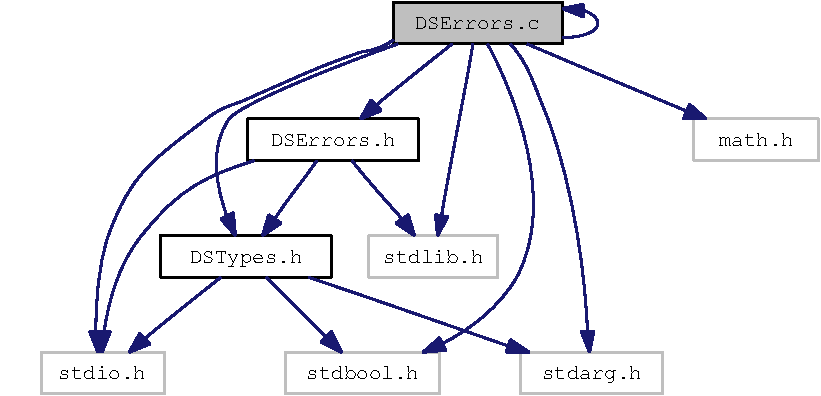
\includegraphics[width=308pt]{_d_s_errors_8c__incl}
\end{center}
\end{figure}
\subsection*{Defines}
\begin{DoxyCompactItemize}
\item 
\#define \hyperlink{_d_s_errors_8c_af86fc5cdaf2e11d46f2aa2201d74f0a4}{STACK\_\-TRACE\_\-NUM}~10
\begin{DoxyCompactList}\small\item\em Maximum number of traces on the call stack. \item\end{DoxyCompactList}\item 
\#define \hyperlink{_d_s_errors_8c_a849adc9d20371988bb26f86618fa75ba}{MSIZE}~1500
\begin{DoxyCompactList}\small\item\em The maximum size of the error message string. \item\end{DoxyCompactList}\end{DoxyCompactItemize}
\subsection*{Functions}
\begin{DoxyCompactItemize}
\item 
void \hyperlink{_d_s_errors_8c_a363f9c264b785ec509da1b11af9ae314}{DSErrorFunction} (const char $\ast$M\_\-DS\_\-Message, char A\_\-DS\_\-ACTION, const char $\ast$FILEN, int LINE, const char $\ast$FUNC)
\begin{DoxyCompactList}\small\item\em Implicit error handling function. Called by DSError which automatically adds file and line arguments. \item\end{DoxyCompactList}\end{DoxyCompactItemize}


\subsection{Detailed Description}
Implementation file with functions for error and exception handling. This file specifies the design space standard for error handling. Contained here are the necessary macros and functions to report the errors throughout the design space library. The DSErrorFunction allows different behaviors; the default behavior, errors are printed to the DSIOErrorFile, which is set to stderr by default. This behavior can be changed by setting changing DSPostWarning, DSPostError and DSPostFatalError function pointers.

\begin{DoxySeeAlso}{See also}
\hyperlink{_d_s_i_o_8h_af8405bae84409f99d5fa564ebaff4c91}{DSIOErrorFile} 

\hyperlink{_d_s_i_o_8h_af12cf032b729ba022698fadaccfea33d}{DSPostWarning} 

\hyperlink{_d_s_i_o_8h_a40c3f80fe9e5002beb7d258e4f89c8d2}{DSPostError} 

\hyperlink{_d_s_i_o_8h_a41b7b42028f3c25f17ca479154c7492d}{DSPostFatalError}
\end{DoxySeeAlso}
Copyright (C) 2011 Jason Lomnitz.\par
\par


This file is part of the Design Space Toolbox V2 (C Library).

The Design Space Toolbox V2 is free software: you can redistribute it and/or modify it under the terms of the GNU General Public License as published by the Free Software Foundation, either version 3 of the License, or (at your option) any later version.

The Design Space Toolbox V2 is distributed in the hope that it will be useful, but WITHOUT ANY WARRANTY; without even the implied warranty of MERCHANTABILITY or FITNESS FOR A PARTICULAR PURPOSE. See the GNU General Public License for more details.

You should have received a copy of the GNU General Public License along with the Design Space Toolbox. If not, see $<$\href{http://www.gnu.org/licenses/}{\tt http://www.gnu.org/licenses/}$>$.

\begin{DoxyAuthor}{Author}
Jason Lomnitz. 
\end{DoxyAuthor}
\begin{DoxyDate}{Date}
2011
\end{DoxyDate}
\begin{Desc}
\item[\hyperlink{todo__todo000001}{Todo}]Implement locks when making the error strings. \end{Desc}


\subsection{Define Documentation}
\hypertarget{_d_s_errors_8c_a849adc9d20371988bb26f86618fa75ba}{
\index{DSErrors.c@{DSErrors.c}!MSIZE@{MSIZE}}
\index{MSIZE@{MSIZE}!DSErrors.c@{DSErrors.c}}
\subsubsection[{MSIZE}]{\setlength{\rightskip}{0pt plus 5cm}\#define MSIZE~1500}}
\label{_d_s_errors_8c_a849adc9d20371988bb26f86618fa75ba}


The maximum size of the error message string. 

This represents the maximum number of characters that an error string can contain. The error string is a statically allocated string. \hypertarget{_d_s_errors_8c_af86fc5cdaf2e11d46f2aa2201d74f0a4}{
\index{DSErrors.c@{DSErrors.c}!STACK\_\-TRACE\_\-NUM@{STACK\_\-TRACE\_\-NUM}}
\index{STACK\_\-TRACE\_\-NUM@{STACK\_\-TRACE\_\-NUM}!DSErrors.c@{DSErrors.c}}
\subsubsection[{STACK\_\-TRACE\_\-NUM}]{\setlength{\rightskip}{0pt plus 5cm}\#define STACK\_\-TRACE\_\-NUM~10}}
\label{_d_s_errors_8c_af86fc5cdaf2e11d46f2aa2201d74f0a4}


Maximum number of traces on the call stack. 

This number represents the maximum number of traces on the call stack that the DSError function adds to the error string. The trace represents all the functions called up to the error. 

\subsection{Function Documentation}
\hypertarget{_d_s_errors_8c_a363f9c264b785ec509da1b11af9ae314}{
\index{DSErrors.c@{DSErrors.c}!DSErrorFunction@{DSErrorFunction}}
\index{DSErrorFunction@{DSErrorFunction}!DSErrors.c@{DSErrors.c}}
\subsubsection[{DSErrorFunction}]{\setlength{\rightskip}{0pt plus 5cm}void DSErrorFunction (const char $\ast$ {\em M\_\-DS\_\-Message}, \/  char {\em A\_\-DS\_\-ACTION}, \/  const char $\ast$ {\em FILEN}, \/  int {\em LINE}, \/  const char $\ast$ {\em FUNC})}}
\label{_d_s_errors_8c_a363f9c264b785ec509da1b11af9ae314}


Implicit error handling function. Called by DSError which automatically adds file and line arguments. 

This function is called implicity when using the DSError macro. The DSError adds the FILE, LINE and FUNC arguments, to report the error/warning at the appropriate file, line and function.


\begin{DoxyParams}{Parameters}
\item[{\em M\_\-DS\_\-Message}]A string containing the error message. \item[{\em A\_\-DS\_\-ACTION}]A character representing an error code as described in A\_\-DS\_\-Actions. \item[{\em FILEN}]A string with the name of the file where the error was reported. \item[{\em LINE}]An integer with the line number in the file where the error was reported. \item[{\em FUNC}]A string with the name of the function where the error was reported.\end{DoxyParams}
\begin{DoxySeeAlso}{See also}
\hyperlink{_d_s_errors_8h_a09b28eb2b01986855910ca97dfe91144}{DSError} 

\hyperlink{group___a___d_s___actions}{Actions for DS Errors.} 
\end{DoxySeeAlso}

\hypertarget{_d_s_errors_8h}{
\section{DSErrors.h File Reference}
\label{_d_s_errors_8h}\index{DSErrors.h@{DSErrors.h}}
}


Header file with functions for error and exception handling.  


{\ttfamily \#include $<$stdio.h$>$}\par
{\ttfamily \#include $<$stdlib.h$>$}\par
{\ttfamily \#include \char`\"{}DSTypes.h\char`\"{}}\par
{\ttfamily \#include \char`\"{}DSIO.h\char`\"{}}\par
Include dependency graph for DSErrors.h:\nopagebreak
\begin{figure}[H]
\begin{center}
\leavevmode
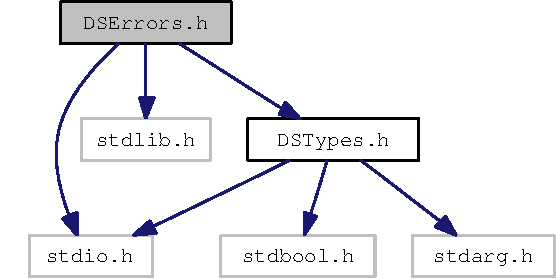
\includegraphics[width=179pt]{_d_s_errors_8h__incl}
\end{center}
\end{figure}
This graph shows which files directly or indirectly include this file:\nopagebreak
\begin{figure}[H]
\begin{center}
\leavevmode
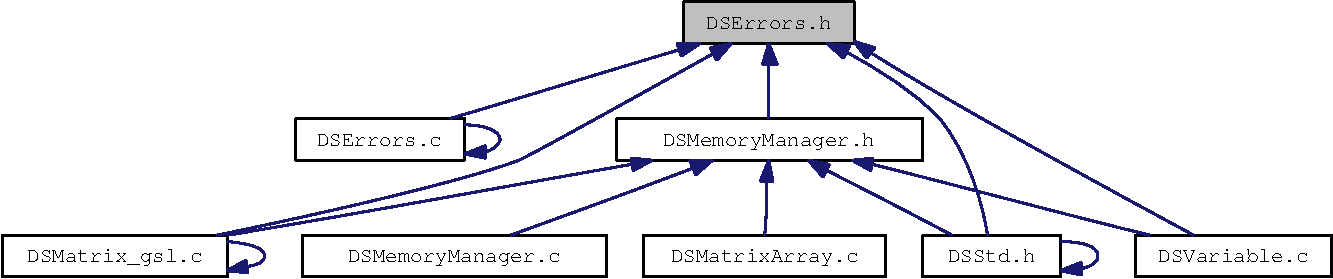
\includegraphics[width=337pt]{_d_s_errors_8h__dep__incl}
\end{center}
\end{figure}
\subsection*{Defines}
\begin{DoxyCompactItemize}
\item 
\hypertarget{group___m___d_s___messages_gadd043ccc956aaee49b9c646f940c167b}{
\#define \hyperlink{group___m___d_s___messages_gadd043ccc956aaee49b9c646f940c167b}{M\_\-DS\_\-NOFILE}~\char`\"{}File not found\char`\"{}}
\label{group___m___d_s___messages_gadd043ccc956aaee49b9c646f940c167b}

\begin{DoxyCompactList}\small\item\em Message for no file found. \item\end{DoxyCompactList}\item 
\hypertarget{group___m___d_s___messages_ga0d502db70be066b76fa94dc1eb9ef75c}{
\#define \hyperlink{group___m___d_s___messages_ga0d502db70be066b76fa94dc1eb9ef75c}{M\_\-DS\_\-NULL}~\char`\"{}NULL pointer\char`\"{}}
\label{group___m___d_s___messages_ga0d502db70be066b76fa94dc1eb9ef75c}

\begin{DoxyCompactList}\small\item\em Message for NULL pointer. \item\end{DoxyCompactList}\item 
\hypertarget{group___m___d_s___messages_ga05191be522c29caa6f80baddfb2a109c}{
\#define \hyperlink{group___m___d_s___messages_ga05191be522c29caa6f80baddfb2a109c}{M\_\-DS\_\-NOFORMAT}~\char`\"{}Format not known\char`\"{}}
\label{group___m___d_s___messages_ga05191be522c29caa6f80baddfb2a109c}

\begin{DoxyCompactList}\small\item\em Message for unknown format. \item\end{DoxyCompactList}\item 
\hypertarget{_d_s_errors_8h_a09ad9583c7a29550cc6a9a7606bf71fb}{
\#define \hyperlink{_d_s_errors_8h_a09ad9583c7a29550cc6a9a7606bf71fb}{M\_\-DS\_\-WRONG}~\char`\"{}Inconsistent data\char`\"{}}
\label{_d_s_errors_8h_a09ad9583c7a29550cc6a9a7606bf71fb}

\begin{DoxyCompactList}\small\item\em Message for inconsistent data being used. \item\end{DoxyCompactList}\item 
\hypertarget{group___m___d_s___messages_ga33ff33533363ff94af03b832587f47c6}{
\#define \hyperlink{group___m___d_s___messages_ga33ff33533363ff94af03b832587f47c6}{M\_\-DS\_\-EXISTS}~\char`\"{}Data already exists\char`\"{}}
\label{group___m___d_s___messages_ga33ff33533363ff94af03b832587f47c6}

\begin{DoxyCompactList}\small\item\em Message for data aleady existing. \item\end{DoxyCompactList}\item 
\hypertarget{_d_s_errors_8h_afd9c8dc0e9bf6bdaa09c3edd3125fc89}{
\#define \hyperlink{_d_s_errors_8h_afd9c8dc0e9bf6bdaa09c3edd3125fc89}{M\_\-DS\_\-NOTHREAD}~\char`\"{}Thread not created\char`\"{}}
\label{_d_s_errors_8h_afd9c8dc0e9bf6bdaa09c3edd3125fc89}

\begin{DoxyCompactList}\small\item\em Message for no thread created. \item\end{DoxyCompactList}\item 
\hypertarget{group___m___d_s___messages_ga47106b8852d8baaf66a0e7f9bd67d36b}{
\#define \hyperlink{group___m___d_s___messages_ga47106b8852d8baaf66a0e7f9bd67d36b}{M\_\-DS\_\-MALLOC}~\char`\"{}Memory alloc failed\char`\"{}}
\label{group___m___d_s___messages_ga47106b8852d8baaf66a0e7f9bd67d36b}

\begin{DoxyCompactList}\small\item\em Message for failure to allocate data. \item\end{DoxyCompactList}\item 
\hypertarget{group___m___d_s___messages_ga79c48eacc7951aa68e4d094f0989faac}{
\#define \hyperlink{group___m___d_s___messages_ga79c48eacc7951aa68e4d094f0989faac}{M\_\-DS\_\-NOT\_\-IMPL}~\char`\"{}Functionality not implemented\char`\"{}}
\label{group___m___d_s___messages_ga79c48eacc7951aa68e4d094f0989faac}

\begin{DoxyCompactList}\small\item\em Message for a feature not yet implemented. \item\end{DoxyCompactList}\item 
\hypertarget{group___a___d_s___actions_ga83fd1c7379ac085b8a9550b8d64f3449}{
\#define \hyperlink{group___a___d_s___actions_ga83fd1c7379ac085b8a9550b8d64f3449}{A\_\-DS\_\-NOERROR}~0}
\label{group___a___d_s___actions_ga83fd1c7379ac085b8a9550b8d64f3449}

\begin{DoxyCompactList}\small\item\em Value for no error. \item\end{DoxyCompactList}\item 
\hypertarget{group___a___d_s___actions_gad61c12e433c47da75f4322d9358c3617}{
\#define \hyperlink{group___a___d_s___actions_gad61c12e433c47da75f4322d9358c3617}{A\_\-DS\_\-WARN}~-\/1}
\label{group___a___d_s___actions_gad61c12e433c47da75f4322d9358c3617}

\begin{DoxyCompactList}\small\item\em Value for a warning. \item\end{DoxyCompactList}\item 
\hypertarget{group___a___d_s___actions_gabaa9a22cc1abc78916b99695489f8df8}{
\#define \hyperlink{group___a___d_s___actions_gabaa9a22cc1abc78916b99695489f8df8}{A\_\-DS\_\-ERROR}~-\/2}
\label{group___a___d_s___actions_gabaa9a22cc1abc78916b99695489f8df8}

\begin{DoxyCompactList}\small\item\em Value for an error. \item\end{DoxyCompactList}\item 
\hypertarget{group___a___d_s___actions_gad3e083f0c8d34073d3597724c2a264f6}{
\#define \hyperlink{group___a___d_s___actions_gad3e083f0c8d34073d3597724c2a264f6}{A\_\-DS\_\-FATAL}~-\/3}
\label{group___a___d_s___actions_gad3e083f0c8d34073d3597724c2a264f6}

\begin{DoxyCompactList}\small\item\em Value for a fatal error, kills program. \item\end{DoxyCompactList}\item 
\hypertarget{_d_s_errors_8h_afc6d540dbb27b62f52427a845a33212f}{
\#define \hyperlink{_d_s_errors_8h_afc6d540dbb27b62f52427a845a33212f}{A\_\-DS\_\-KILLNOW}~A\_\-DS\_\-FATAL}
\label{_d_s_errors_8h_afc6d540dbb27b62f52427a845a33212f}

\begin{DoxyCompactList}\small\item\em DEPRECATED: \item\end{DoxyCompactList}\item 
\#define \hyperlink{_d_s_errors_8h_a09b28eb2b01986855910ca97dfe91144}{DSError}(M\_\-DS\_\-Message, A\_\-DS\_\-Action)~DSErrorFunction(M\_\-DS\_\-Message, A\_\-DS\_\-Action, \_\-\_\-FILE\_\-\_\-, \_\-\_\-LINE\_\-\_\-, \_\-\_\-func\_\-\_\-)
\begin{DoxyCompactList}\small\item\em Error reporting macro. \item\end{DoxyCompactList}\end{DoxyCompactItemize}
\subsection*{Functions}
\begin{DoxyCompactItemize}
\item 
\hypertarget{_d_s_errors_8h_a71b6e7a909b430863f1a850122a17f78}{
\_\-\_\-deprecated void {\bfseries DSErrorSetPrintFunction} (void($\ast$function)(const char $\ast$restrict))}
\label{_d_s_errors_8h_a71b6e7a909b430863f1a850122a17f78}

\item 
\hypertarget{_d_s_errors_8h_a3b412662349f03e9fc9fbb782ec3b373}{
\_\-\_\-deprecated void {\bfseries DSErrorSetErrorFile} (FILE $\ast$aFile)}
\label{_d_s_errors_8h_a3b412662349f03e9fc9fbb782ec3b373}

\item 
void \hyperlink{_d_s_errors_8h_a363f9c264b785ec509da1b11af9ae314}{DSErrorFunction} (const char $\ast$M\_\-DS\_\-Message, char A\_\-DS\_\-ACTION, const char $\ast$FILEN, int LINE, const char $\ast$FUNC)
\begin{DoxyCompactList}\small\item\em Implicit error handling function. Called by DSError which automatically adds file and line arguments. \item\end{DoxyCompactList}\end{DoxyCompactItemize}


\subsection{Detailed Description}
Header file with functions for error and exception handling. This file specifies the design space standard for error handling. Contained here are the necessary macros and functions to succesfully report the errors throughout the design space library.

Copyright (C) 2011 Jason Lomnitz.\par
\par


This file is part of the Design Space Toolbox V2 (C Library).

The Design Space Toolbox V2 is free software: you can redistribute it and/or modify it under the terms of the GNU General Public License as published by the Free Software Foundation, either version 3 of the License, or (at your option) any later version.

The Design Space Toolbox V2 is distributed in the hope that it will be useful, but WITHOUT ANY WARRANTY; without even the implied warranty of MERCHANTABILITY or FITNESS FOR A PARTICULAR PURPOSE. See the GNU General Public License for more details.

You should have received a copy of the GNU General Public License along with the Design Space Toolbox. If not, see $<$\href{http://www.gnu.org/licenses/}{\tt http://www.gnu.org/licenses/}$>$.

\begin{DoxyAuthor}{Author}
Jason Lomnitz. 
\end{DoxyAuthor}
\begin{DoxyDate}{Date}
2011 
\end{DoxyDate}


\subsection{Define Documentation}
\hypertarget{_d_s_errors_8h_a09b28eb2b01986855910ca97dfe91144}{
\index{DSErrors.h@{DSErrors.h}!DSError@{DSError}}
\index{DSError@{DSError}!DSErrors.h@{DSErrors.h}}
\subsubsection[{DSError}]{\setlength{\rightskip}{0pt plus 5cm}\#define DSError(M\_\-DS\_\-Message, \/  A\_\-DS\_\-Action)~DSErrorFunction(M\_\-DS\_\-Message, A\_\-DS\_\-Action, \_\-\_\-FILE\_\-\_\-, \_\-\_\-LINE\_\-\_\-, \_\-\_\-func\_\-\_\-)}}
\label{_d_s_errors_8h_a09b28eb2b01986855910ca97dfe91144}


Error reporting macro. 

Definition of the error reporting macro used within the DesignSpace C toolbox, this is a define which takes a string, which may be a standard message, and an action and reports it via the standard warning and error posting functions in the standard IO functions. A default behavior of the DSError macro posts warning and errors to stderr, while a fatal error posts the error to stderr and aborts the program.

\begin{DoxySeeAlso}{See also}
\hyperlink{_d_s_i_o_8h_af12cf032b729ba022698fadaccfea33d}{DSPostWarning} 

\hyperlink{_d_s_i_o_8h_a40c3f80fe9e5002beb7d258e4f89c8d2}{DSPostError} 

\hyperlink{_d_s_i_o_8h_a41b7b42028f3c25f17ca479154c7492d}{DSPostFatalError}

\hyperlink{group___m___d_s___messages}{Messages for DS Errors.} 

\hyperlink{group___a___d_s___actions}{Actions for DS Errors.} 
\end{DoxySeeAlso}


\subsection{Function Documentation}
\hypertarget{_d_s_errors_8h_a363f9c264b785ec509da1b11af9ae314}{
\index{DSErrors.h@{DSErrors.h}!DSErrorFunction@{DSErrorFunction}}
\index{DSErrorFunction@{DSErrorFunction}!DSErrors.h@{DSErrors.h}}
\subsubsection[{DSErrorFunction}]{\setlength{\rightskip}{0pt plus 5cm}void DSErrorFunction (const char $\ast$ {\em M\_\-DS\_\-Message}, \/  char {\em A\_\-DS\_\-ACTION}, \/  const char $\ast$ {\em FILEN}, \/  int {\em LINE}, \/  const char $\ast$ {\em FUNC})}}
\label{_d_s_errors_8h_a363f9c264b785ec509da1b11af9ae314}


Implicit error handling function. Called by DSError which automatically adds file and line arguments. 

This function is called implicity when using the DSError macro. The DSError adds the FILE and LINE argument, to report the error/warning at the appropriate file and line.

\begin{DoxySeeAlso}{See also}
\hyperlink{_d_s_errors_8h_a09b28eb2b01986855910ca97dfe91144}{DSError} 

\hyperlink{group___a___d_s___actions}{Actions for DS Errors.} 
\end{DoxySeeAlso}

\hypertarget{_d_s_expression_8c}{
\section{DSExpression.c File Reference}
\label{_d_s_expression_8c}\index{DSExpression.c@{DSExpression.c}}
}


Implementation file with functions for dealing with mathematical expressions.  


{\ttfamily \#include $<$stdio.h$>$}\par
{\ttfamily \#include $<$string.h$>$}\par
{\ttfamily \#include $<$math.h$>$}\par
{\ttfamily \#include \char`\"{}DSErrors.h\char`\"{}}\par
{\ttfamily \#include \char`\"{}DSMemoryManager.h\char`\"{}}\par
{\ttfamily \#include \char`\"{}DSVariable.h\char`\"{}}\par
{\ttfamily \#include \char`\"{}DSExpression.h\char`\"{}}\par
{\ttfamily \#include \char`\"{}DSExpressionTokenizer.h\char`\"{}}\par
{\ttfamily \#include \char`\"{}DSTypes.h\char`\"{}}\par
Include dependency graph for DSExpression.c:This graph shows which files directly or indirectly include this file:\subsection*{Defines}
\begin{DoxyCompactItemize}
\item 
\hypertarget{_d_s_expression_8c_a56826acaf50d31e4558375e1e482e971}{
\#define {\bfseries DS\_\-EXPRESSION\_\-CONSTANT\_\-BRANCH}~0}
\label{_d_s_expression_8c_a56826acaf50d31e4558375e1e482e971}

\item 
\hypertarget{_d_s_expression_8c_aacce28d2985e154d813e5f9aff6ccaa3}{
\#define {\bfseries DS\_\-EXPRESSION\_\-STRING\_\-INIT\_\-LENGTH}~1000}
\label{_d_s_expression_8c_aacce28d2985e154d813e5f9aff6ccaa3}

\item 
\hypertarget{_d_s_expression_8c_af1511853cea9b840caf04d927801834d}{
\#define {\bfseries ds\_\-function\_\-index\_\-log}~0}
\label{_d_s_expression_8c_af1511853cea9b840caf04d927801834d}

\item 
\hypertarget{_d_s_expression_8c_a30df4998e3a3f763daa0119faa591808}{
\#define {\bfseries ds\_\-function\_\-index\_\-ln}~1}
\label{_d_s_expression_8c_a30df4998e3a3f763daa0119faa591808}

\item 
\hypertarget{_d_s_expression_8c_a4e9a2e9973f5e1c8c9d61c7c4ac1d092}{
\#define {\bfseries ds\_\-function\_\-index\_\-log10}~2}
\label{_d_s_expression_8c_a4e9a2e9973f5e1c8c9d61c7c4ac1d092}

\item 
\hypertarget{_d_s_expression_8c_aa0f67ea20fcc685de99e4760497ba90b}{
\#define {\bfseries ds\_\-function\_\-index\_\-cos}~3}
\label{_d_s_expression_8c_aa0f67ea20fcc685de99e4760497ba90b}

\item 
\hypertarget{_d_s_expression_8c_a5eba39f6be9e7bc4d4b371a79c10db65}{
\#define {\bfseries ds\_\-function\_\-index\_\-sin}~4}
\label{_d_s_expression_8c_a5eba39f6be9e7bc4d4b371a79c10db65}

\end{DoxyCompactItemize}
\subsection*{Functions}
\begin{DoxyCompactItemize}
\item 
\hypertarget{_d_s_expression_8c_a0d3722a222023a8677952bb5aa0b56dd}{
\hyperlink{structdsexpression}{DSExpression} $\ast$ {\bfseries DSExpressionAllocWithOperator} (const char op\_\-code)}
\label{_d_s_expression_8c_a0d3722a222023a8677952bb5aa0b56dd}

\item 
\hypertarget{_d_s_expression_8c_aea7d132c63527347f3e1474312a89126}{
\hyperlink{structdsexpression}{DSExpression} $\ast$ {\bfseries DSExpressionAllocWithConstant} (const double value)}
\label{_d_s_expression_8c_aea7d132c63527347f3e1474312a89126}

\item 
\hypertarget{_d_s_expression_8c_a7801cf181c8c5eb7d47505d9dc98cf4d}{
\hyperlink{structdsexpression}{DSExpression} $\ast$ {\bfseries DSExpressionAllocWithVariableName} (const char $\ast$name)}
\label{_d_s_expression_8c_a7801cf181c8c5eb7d47505d9dc98cf4d}

\item 
\hypertarget{_d_s_expression_8c_a421fb70482a371a9c1cccad85f843a67}{
void {\bfseries DSExpressionFree} (\hyperlink{structdsexpression}{DSExpression} $\ast$root)}
\label{_d_s_expression_8c_a421fb70482a371a9c1cccad85f843a67}

\item 
\hypertarget{_d_s_expression_8c_a6d4867e24915ebd378abd3a9762f350d}{
\hyperlink{structdsexpression}{DSExpression} $\ast$ {\bfseries DSExpressionCopy} (const \hyperlink{structdsexpression}{DSExpression} $\ast$expression)}
\label{_d_s_expression_8c_a6d4867e24915ebd378abd3a9762f350d}

\item 
\hypertarget{_d_s_expression_8c_a179f6a5530ff0852d3e266cf22e535b0}{
\hyperlink{structdsexpression}{DSExpression} $\ast$ {\bfseries DSExpressionByParsingString} (const char $\ast$string)}
\label{_d_s_expression_8c_a179f6a5530ff0852d3e266cf22e535b0}

\item 
\hypertarget{_d_s_expression_8c_a6d563f2b52ae0c1b62416af2eba06425}{
\hyperlink{structdsexpression}{DSExpression} $\ast$ {\bfseries DSExpressionAddExpressions} (\hyperlink{structdsexpression}{DSExpression} $\ast$lvalue, \hyperlink{structdsexpression}{DSExpression} $\ast$rvalue)}
\label{_d_s_expression_8c_a6d563f2b52ae0c1b62416af2eba06425}

\item 
\hypertarget{_d_s_expression_8c_abe72cdb703bcc860b975b8cc4458018e}{
void {\bfseries DSExpressionAddBranch} (\hyperlink{structdsexpression}{DSExpression} $\ast$expression, \hyperlink{structdsexpression}{DSExpression} $\ast$branch)}
\label{_d_s_expression_8c_abe72cdb703bcc860b975b8cc4458018e}

\item 
\hypertarget{_d_s_expression_8c_a0ab75800267c17508893a11a900e2e36}{
double {\bfseries DSExpressionEvaluateWithVariablePool} (const \hyperlink{structdsexpression}{DSExpression} $\ast$expression, const \hyperlink{struct_d_s_variable_pool}{DSVariablePool} $\ast$pool)}
\label{_d_s_expression_8c_a0ab75800267c17508893a11a900e2e36}

\item 
\hypertarget{_d_s_expression_8c_aecf7720bc7fff6cacde0a5e27df83074}{
char $\ast$ {\bfseries DSExpressionAsString} (const \hyperlink{structdsexpression}{DSExpression} $\ast$expression)}
\label{_d_s_expression_8c_aecf7720bc7fff6cacde0a5e27df83074}

\item 
\hypertarget{_d_s_expression_8c_a255aad510b69f8a0691ccff4ad3702c9}{
char $\ast$ {\bfseries DSExpressionAsTroffString} (const \hyperlink{structdsexpression}{DSExpression} $\ast$expression)}
\label{_d_s_expression_8c_a255aad510b69f8a0691ccff4ad3702c9}

\item 
\hypertarget{_d_s_expression_8c_a9bb539af87116d9890053b0fcc710ced}{
void {\bfseries DSExpressionPrint} (const \hyperlink{structdsexpression}{DSExpression} $\ast$expression)}
\label{_d_s_expression_8c_a9bb539af87116d9890053b0fcc710ced}

\end{DoxyCompactItemize}


\subsection{Detailed Description}
Implementation file with functions for dealing with mathematical expressions. Copyright (C) 2011 Jason Lomnitz.\par
\par


This file is part of the Design Space Toolbox V2 (C Library).

The Design Space Toolbox V2 is free software: you can redistribute it and/or modify it under the terms of the GNU General Public License as published by the Free Software Foundation, either version 3 of the License, or (at your option) any later version.

The Design Space Toolbox V2 is distributed in the hope that it will be useful, but WITHOUT ANY WARRANTY; without even the implied warranty of MERCHANTABILITY or FITNESS FOR A PARTICULAR PURPOSE. See the GNU General Public License for more details.

You should have received a copy of the GNU General Public License along with the Design Space Toolbox. If not, see $<$\href{http://www.gnu.org/licenses/}{\tt http://www.gnu.org/licenses/}$>$.

\begin{DoxyAuthor}{Author}
Jason Lomnitz. 
\end{DoxyAuthor}
\begin{DoxyDate}{Date}
2011 
\end{DoxyDate}

\hypertarget{_d_s_expression_8h}{
\section{DSExpression.h File Reference}
\label{_d_s_expression_8h}\index{DSExpression.h@{DSExpression.h}}
}


Header file with functions for dealing with mathematical expressions.  


{\ttfamily \#include \char`\"{}DSTypes.h\char`\"{}}\par
Include dependency graph for DSExpression.h:This graph shows which files directly or indirectly include this file:\subsection*{Defines}
\begin{DoxyCompactItemize}
\item 
\hypertarget{_d_s_expression_8h_a018e4498b5023777c3316b3d06779af6}{
\#define {\bfseries DS\_\-EXPRESSION\_\-TYPE\_\-UNDEFINED}~0}
\label{_d_s_expression_8h_a018e4498b5023777c3316b3d06779af6}

\item 
\hypertarget{_d_s_expression_8h_a52c5f265c27f174b5862253bbd2bafbc}{
\#define {\bfseries DS\_\-EXPRESSION\_\-TYPE\_\-OPERATOR}~1}
\label{_d_s_expression_8h_a52c5f265c27f174b5862253bbd2bafbc}

\item 
\hypertarget{_d_s_expression_8h_a521d0799b0b6c950e69f94fb7d492c8a}{
\#define {\bfseries DS\_\-EXPRESSION\_\-TYPE\_\-CONSTANT}~2}
\label{_d_s_expression_8h_a521d0799b0b6c950e69f94fb7d492c8a}

\item 
\hypertarget{_d_s_expression_8h_a2ad8725730cc1dd4a1bd121c6d0a30bf}{
\#define {\bfseries DS\_\-EXPRESSION\_\-TYPE\_\-VARIABLE}~3}
\label{_d_s_expression_8h_a2ad8725730cc1dd4a1bd121c6d0a30bf}

\item 
\hypertarget{_d_s_expression_8h_a7cb9ccc7c5be2415c750a0bef744ac6e}{
\#define {\bfseries DS\_\-EXPRESSION\_\-TYPE\_\-FUNCTION}~4}
\label{_d_s_expression_8h_a7cb9ccc7c5be2415c750a0bef744ac6e}

\item 
\hypertarget{_d_s_expression_8h_af51632ada2fed1e2313c4e40c226e1d6}{
\#define {\bfseries DSExpressionSetOperator}(x, y)~((x-\/$>$node.op\_\-code) = y, (x-\/$>$type = DS\_\-EXPRESSION\_\-TYPE\_\-OPERATOR))}
\label{_d_s_expression_8h_af51632ada2fed1e2313c4e40c226e1d6}

\item 
\hypertarget{_d_s_expression_8h_ab3b520fd7d0dfac38ae7f6bb13c824fb}{
\#define {\bfseries DSExpressionSetVariable}(x, y)~((x-\/$>$node.variable) = y, (x-\/$>$type = DS\_\-EXPRESSION\_\-TYPE\_\-VARIABLE))}
\label{_d_s_expression_8h_ab3b520fd7d0dfac38ae7f6bb13c824fb}

\item 
\hypertarget{_d_s_expression_8h_af5535e79fde8eab01648730aee62da14}{
\#define {\bfseries DSExpressionSetConstant}(x, y)~((x-\/$>$node.constant) = y, (x-\/$>$type = DS\_\-EXPRESSION\_\-TYPE\_\-CONSTANT))}
\label{_d_s_expression_8h_af5535e79fde8eab01648730aee62da14}

\item 
\hypertarget{_d_s_expression_8h_a99efea0eeb9a6e5d763b023c644d73a1}{
\#define {\bfseries DSExpressionType}(x)~(x-\/$>$type)}
\label{_d_s_expression_8h_a99efea0eeb9a6e5d763b023c644d73a1}

\item 
\hypertarget{_d_s_expression_8h_a5ee5d9e809898d3496d2cd2ed314c511}{
\#define {\bfseries DSExpressionNumberOfBranches}(x)~(x-\/$>$numberOfBranches)}
\label{_d_s_expression_8h_a5ee5d9e809898d3496d2cd2ed314c511}

\item 
\hypertarget{_d_s_expression_8h_a67ca4ff30059f1a82e27ac4a8e906ae1}{
\#define {\bfseries DSExpressionBranchAtIndex}(x, y)~((y $<$ DSExpressionNumberOfBranches(x)) ? x-\/$>$branches\mbox{[}y\mbox{]} : NULL)}
\label{_d_s_expression_8h_a67ca4ff30059f1a82e27ac4a8e906ae1}

\item 
\hypertarget{_d_s_expression_8h_ae0151e3213caca6ce5ac85a5236386cf}{
\#define {\bfseries DSExpressionOperator}(x)~((x-\/$>$type == DS\_\-EXPRESSION\_\-TYPE\_\-OPERATOR) ? x-\/$>$node.op\_\-code : '?')}
\label{_d_s_expression_8h_ae0151e3213caca6ce5ac85a5236386cf}

\item 
\hypertarget{_d_s_expression_8h_a98dcd8a603ecdcb86c19f213dcf2b792}{
\#define {\bfseries DSExpressionVariable}(x)~((x-\/$>$type == DS\_\-EXPRESSION\_\-TYPE\_\-VARIABLE $|$$|$ x-\/$>$type == DS\_\-EXPRESSION\_\-TYPE\_\-FUNCTION) ? x-\/$>$node.variable : NULL)}
\label{_d_s_expression_8h_a98dcd8a603ecdcb86c19f213dcf2b792}

\item 
\hypertarget{_d_s_expression_8h_a73e36aab11049ec9c16184c885be3e1e}{
\#define {\bfseries DSExpressionConstant}(x)~((x-\/$>$type == DS\_\-EXPRESSION\_\-TYPE\_\-CONSTANT) ? x-\/$>$node.constant : NAN)}
\label{_d_s_expression_8h_a73e36aab11049ec9c16184c885be3e1e}

\end{DoxyCompactItemize}
\subsection*{Functions}
\begin{DoxyCompactItemize}
\item 
\hypertarget{_d_s_expression_8h_a0d3722a222023a8677952bb5aa0b56dd}{
\hyperlink{structdsexpression}{DSExpression} $\ast$ {\bfseries DSExpressionAllocWithOperator} (const char op\_\-code)}
\label{_d_s_expression_8h_a0d3722a222023a8677952bb5aa0b56dd}

\item 
\hypertarget{_d_s_expression_8h_aea7d132c63527347f3e1474312a89126}{
\hyperlink{structdsexpression}{DSExpression} $\ast$ {\bfseries DSExpressionAllocWithConstant} (const double value)}
\label{_d_s_expression_8h_aea7d132c63527347f3e1474312a89126}

\item 
\hypertarget{_d_s_expression_8h_a7801cf181c8c5eb7d47505d9dc98cf4d}{
\hyperlink{structdsexpression}{DSExpression} $\ast$ {\bfseries DSExpressionAllocWithVariableName} (const char $\ast$name)}
\label{_d_s_expression_8h_a7801cf181c8c5eb7d47505d9dc98cf4d}

\item 
\hypertarget{_d_s_expression_8h_a421fb70482a371a9c1cccad85f843a67}{
void {\bfseries DSExpressionFree} (\hyperlink{structdsexpression}{DSExpression} $\ast$root)}
\label{_d_s_expression_8h_a421fb70482a371a9c1cccad85f843a67}

\item 
\hypertarget{_d_s_expression_8h_a6d4867e24915ebd378abd3a9762f350d}{
\hyperlink{structdsexpression}{DSExpression} $\ast$ {\bfseries DSExpressionCopy} (const \hyperlink{structdsexpression}{DSExpression} $\ast$expression)}
\label{_d_s_expression_8h_a6d4867e24915ebd378abd3a9762f350d}

\item 
\hypertarget{_d_s_expression_8h_a179f6a5530ff0852d3e266cf22e535b0}{
\hyperlink{structdsexpression}{DSExpression} $\ast$ {\bfseries DSExpressionByParsingString} (const char $\ast$string)}
\label{_d_s_expression_8h_a179f6a5530ff0852d3e266cf22e535b0}

\item 
\hypertarget{_d_s_expression_8h_a6d563f2b52ae0c1b62416af2eba06425}{
\hyperlink{structdsexpression}{DSExpression} $\ast$ {\bfseries DSExpressionAddExpressions} (\hyperlink{structdsexpression}{DSExpression} $\ast$lvalue, \hyperlink{structdsexpression}{DSExpression} $\ast$rvalue)}
\label{_d_s_expression_8h_a6d563f2b52ae0c1b62416af2eba06425}

\item 
\hypertarget{_d_s_expression_8h_a0ab75800267c17508893a11a900e2e36}{
double {\bfseries DSExpressionEvaluateWithVariablePool} (const \hyperlink{structdsexpression}{DSExpression} $\ast$expression, const \hyperlink{struct_d_s_variable_pool}{DSVariablePool} $\ast$pool)}
\label{_d_s_expression_8h_a0ab75800267c17508893a11a900e2e36}

\item 
\hypertarget{_d_s_expression_8h_aecf7720bc7fff6cacde0a5e27df83074}{
char $\ast$ {\bfseries DSExpressionAsString} (const \hyperlink{structdsexpression}{DSExpression} $\ast$expression)}
\label{_d_s_expression_8h_aecf7720bc7fff6cacde0a5e27df83074}

\item 
\hypertarget{_d_s_expression_8h_a255aad510b69f8a0691ccff4ad3702c9}{
char $\ast$ {\bfseries DSExpressionAsTroffString} (const \hyperlink{structdsexpression}{DSExpression} $\ast$expression)}
\label{_d_s_expression_8h_a255aad510b69f8a0691ccff4ad3702c9}

\item 
\hypertarget{_d_s_expression_8h_a9bb539af87116d9890053b0fcc710ced}{
void {\bfseries DSExpressionPrint} (const \hyperlink{structdsexpression}{DSExpression} $\ast$expression)}
\label{_d_s_expression_8h_a9bb539af87116d9890053b0fcc710ced}

\end{DoxyCompactItemize}


\subsection{Detailed Description}
Header file with functions for dealing with mathematical expressions. The mathematical expressions are converted into a form similar to the model used in MUPAD. Internally, only three operators are used: '+', '$\ast$' and '$^\wedge$'. The '-\/' operator is converted, such that \$A-\/B\$ would actually be \$A+B$\ast$(-\/1)\$ and the '/' operator is converted such that \$A/B\$ would actually be \$A$\ast$B$^\wedge$-\/1\$. The '$\ast$' and '+' operators must have at least two branches, but may have any number of branches. The first branch for these operators is reserved for constant values, such that a+b is actually 0+a+b, and a$\ast$b is actually 1$\ast$a$\ast$b. This canonical form is used to speed up the processing of mathematical expressions when converting them to matrices for the GMA and SSystem. The '$^\wedge$' must have only two branches.

Copyright (C) 2011 Jason Lomnitz.\par
\par


This file is part of the Design Space Toolbox V2 (C Library).

The Design Space Toolbox V2 is free software: you can redistribute it and/or modify it under the terms of the GNU General Public License as published by the Free Software Foundation, either version 3 of the License, or (at your option) any later version.

The Design Space Toolbox V2 is distributed in the hope that it will be useful, but WITHOUT ANY WARRANTY; without even the implied warranty of MERCHANTABILITY or FITNESS FOR A PARTICULAR PURPOSE. See the GNU General Public License for more details.

You should have received a copy of the GNU General Public License along with the Design Space Toolbox. If not, see $<$\href{http://www.gnu.org/licenses/}{\tt http://www.gnu.org/licenses/}$>$.

\begin{DoxyAuthor}{Author}
Jason Lomnitz. 
\end{DoxyAuthor}
\begin{DoxyDate}{Date}
2011 
\end{DoxyDate}

\hypertarget{_d_s_expression_tokenizer_lex_8c}{
\section{DSExpressionTokenizerLex.c File Reference}
\label{_d_s_expression_tokenizer_lex_8c}\index{DSExpressionTokenizerLex.c@{DSExpressionTokenizerLex.c}}
}


Implementation file with functions for tokenizing matrices, generated by flex.  


{\ttfamily \#include $<$stdio.h$>$}\par
{\ttfamily \#include $<$string.h$>$}\par
{\ttfamily \#include $<$errno.h$>$}\par
{\ttfamily \#include $<$stdlib.h$>$}\par
{\ttfamily \#include \char`\"{}DSTypes.h\char`\"{}}\par
{\ttfamily \#include \char`\"{}DSMemoryManager.h\char`\"{}}\par
{\ttfamily \#include \char`\"{}DSExpression.h\char`\"{}}\par
{\ttfamily \#include \char`\"{}DSExpressionTokenizer.h\char`\"{}}\par
{\ttfamily \#include $<$unistd.h$>$}\par
Include dependency graph for DSExpressionTokenizerLex.c:\subsection*{Data Structures}
\begin{DoxyCompactItemize}
\item 
struct \hyperlink{structyy__buffer__state}{yy\_\-buffer\_\-state}
\item 
struct \hyperlink{structyy__trans__info}{yy\_\-trans\_\-info}
\item 
struct \hyperlink{structyyguts__t}{yyguts\_\-t}
\end{DoxyCompactItemize}
\subsection*{Defines}
\begin{DoxyCompactItemize}
\item 
\hypertarget{_d_s_expression_tokenizer_lex_8c_a1ae16e642a197fa4948998525813c6f5}{
\#define {\bfseries YY\_\-INT\_\-ALIGNED}~short int}
\label{_d_s_expression_tokenizer_lex_8c_a1ae16e642a197fa4948998525813c6f5}

\item 
\hypertarget{_d_s_expression_tokenizer_lex_8c_a3c3d1ef92e93b0bc81d7760a73d5c3b6}{
\#define {\bfseries FLEX\_\-SCANNER}}
\label{_d_s_expression_tokenizer_lex_8c_a3c3d1ef92e93b0bc81d7760a73d5c3b6}

\item 
\hypertarget{_d_s_expression_tokenizer_lex_8c_a243ca1d30872935faf05ea5118ed6fdc}{
\#define {\bfseries YY\_\-FLEX\_\-MAJOR\_\-VERSION}~2}
\label{_d_s_expression_tokenizer_lex_8c_a243ca1d30872935faf05ea5118ed6fdc}

\item 
\hypertarget{_d_s_expression_tokenizer_lex_8c_a90f9d458829400869e47efb68a865677}{
\#define {\bfseries YY\_\-FLEX\_\-MINOR\_\-VERSION}~5}
\label{_d_s_expression_tokenizer_lex_8c_a90f9d458829400869e47efb68a865677}

\item 
\hypertarget{_d_s_expression_tokenizer_lex_8c_ac676bd06869180ea493e9b6d7c078dbb}{
\#define {\bfseries YY\_\-FLEX\_\-SUBMINOR\_\-VERSION}~35}
\label{_d_s_expression_tokenizer_lex_8c_ac676bd06869180ea493e9b6d7c078dbb}

\item 
\hypertarget{_d_s_expression_tokenizer_lex_8c_a9465c9986fdda27730c9dff8d16a0887}{
\#define {\bfseries FLEX\_\-BETA}}
\label{_d_s_expression_tokenizer_lex_8c_a9465c9986fdda27730c9dff8d16a0887}

\item 
\hypertarget{_d_s_expression_tokenizer_lex_8c_ad4e9955955b27624963643eac448118a}{
\#define {\bfseries INT16\_\-MIN}~(-\/32767-\/1)}
\label{_d_s_expression_tokenizer_lex_8c_ad4e9955955b27624963643eac448118a}

\item 
\hypertarget{_d_s_expression_tokenizer_lex_8c_a688eb21a22db27c2b2bd5836943cdcbe}{
\#define {\bfseries INT32\_\-MIN}~(-\/2147483647-\/1)}
\label{_d_s_expression_tokenizer_lex_8c_a688eb21a22db27c2b2bd5836943cdcbe}

\item 
\hypertarget{_d_s_expression_tokenizer_lex_8c_aaf7f29f45f1a513b4748a4e5014ddf6a}{
\#define {\bfseries INT8\_\-MAX}~(127)}
\label{_d_s_expression_tokenizer_lex_8c_aaf7f29f45f1a513b4748a4e5014ddf6a}

\item 
\hypertarget{_d_s_expression_tokenizer_lex_8c_ac58f2c111cc9989c86db2a7dc4fd84ca}{
\#define {\bfseries INT16\_\-MAX}~(32767)}
\label{_d_s_expression_tokenizer_lex_8c_ac58f2c111cc9989c86db2a7dc4fd84ca}

\item 
\hypertarget{_d_s_expression_tokenizer_lex_8c_a181807730d4a375f848ba139813ce04f}{
\#define {\bfseries INT32\_\-MAX}~(2147483647)}
\label{_d_s_expression_tokenizer_lex_8c_a181807730d4a375f848ba139813ce04f}

\item 
\hypertarget{_d_s_expression_tokenizer_lex_8c_aeb4e270a084ee26fe73e799861bd0252}{
\#define {\bfseries UINT8\_\-MAX}~(255U)}
\label{_d_s_expression_tokenizer_lex_8c_aeb4e270a084ee26fe73e799861bd0252}

\item 
\hypertarget{_d_s_expression_tokenizer_lex_8c_a3ea490c9b3617d4479bd80ef93cd5602}{
\#define {\bfseries UINT16\_\-MAX}~(65535U)}
\label{_d_s_expression_tokenizer_lex_8c_a3ea490c9b3617d4479bd80ef93cd5602}

\item 
\hypertarget{_d_s_expression_tokenizer_lex_8c_ab5eb23180f7cc12b7d6c04a8ec067fdd}{
\#define {\bfseries UINT32\_\-MAX}~(4294967295U)}
\label{_d_s_expression_tokenizer_lex_8c_ab5eb23180f7cc12b7d6c04a8ec067fdd}

\item 
\hypertarget{_d_s_expression_tokenizer_lex_8c_aa2f1a918be586b44bf08126bde2d7cc9}{
\#define {\bfseries yyconst}}
\label{_d_s_expression_tokenizer_lex_8c_aa2f1a918be586b44bf08126bde2d7cc9}

\item 
\hypertarget{_d_s_expression_tokenizer_lex_8c_a8e0bcf8f8a5b613ea583347f8bc31cbf}{
\#define {\bfseries YY\_\-NULL}~0}
\label{_d_s_expression_tokenizer_lex_8c_a8e0bcf8f8a5b613ea583347f8bc31cbf}

\item 
\hypertarget{_d_s_expression_tokenizer_lex_8c_af1185350b7a92cf8aa5324c68850c8a6}{
\#define {\bfseries YY\_\-SC\_\-TO\_\-UI}(c)~((unsigned int) (unsigned char) c)}
\label{_d_s_expression_tokenizer_lex_8c_af1185350b7a92cf8aa5324c68850c8a6}

\item 
\hypertarget{_d_s_expression_tokenizer_lex_8c_a5d5508008cac8fb66fca3baa4e9b6584}{
\#define {\bfseries YY\_\-TYPEDEF\_\-YY\_\-SCANNER\_\-T}}
\label{_d_s_expression_tokenizer_lex_8c_a5d5508008cac8fb66fca3baa4e9b6584}

\item 
\hypertarget{_d_s_expression_tokenizer_lex_8c_aa789f4617e33fb99594cb04a3688a0c1}{
\#define {\bfseries yyin}~yyg-\/$>$yyin\_\-r}
\label{_d_s_expression_tokenizer_lex_8c_aa789f4617e33fb99594cb04a3688a0c1}

\item 
\hypertarget{_d_s_expression_tokenizer_lex_8c_a4fd44867d448dcb6fc32ea004a15de54}{
\#define {\bfseries yyout}~yyg-\/$>$yyout\_\-r}
\label{_d_s_expression_tokenizer_lex_8c_a4fd44867d448dcb6fc32ea004a15de54}

\item 
\hypertarget{_d_s_expression_tokenizer_lex_8c_a6d98927535a334881d37873915fbc45f}{
\#define {\bfseries yyextra}~yyg-\/$>$yyextra\_\-r}
\label{_d_s_expression_tokenizer_lex_8c_a6d98927535a334881d37873915fbc45f}

\item 
\hypertarget{_d_s_expression_tokenizer_lex_8c_afa07a629486cb790560bb95713ec7794}{
\#define {\bfseries yyleng}~yyg-\/$>$yyleng\_\-r}
\label{_d_s_expression_tokenizer_lex_8c_afa07a629486cb790560bb95713ec7794}

\item 
\hypertarget{_d_s_expression_tokenizer_lex_8c_a0d71f919dbec1ffd74b2460fa7e5ac28}{
\#define {\bfseries yytext}~yyg-\/$>$yytext\_\-r}
\label{_d_s_expression_tokenizer_lex_8c_a0d71f919dbec1ffd74b2460fa7e5ac28}

\item 
\hypertarget{_d_s_expression_tokenizer_lex_8c_ad71cf0fddcfe4f61de0929105b33226c}{
\#define {\bfseries yylineno}~(YY\_\-CURRENT\_\-BUFFER\_\-LVALUE-\/$>$yy\_\-bs\_\-lineno)}
\label{_d_s_expression_tokenizer_lex_8c_ad71cf0fddcfe4f61de0929105b33226c}

\item 
\hypertarget{_d_s_expression_tokenizer_lex_8c_adb60e80d603c103e73f2561c7499095c}{
\#define {\bfseries yycolumn}~(YY\_\-CURRENT\_\-BUFFER\_\-LVALUE-\/$>$yy\_\-bs\_\-column)}
\label{_d_s_expression_tokenizer_lex_8c_adb60e80d603c103e73f2561c7499095c}

\item 
\hypertarget{_d_s_expression_tokenizer_lex_8c_a301f4439c9b191c80db45f5b1a8c7269}{
\#define {\bfseries yy\_\-flex\_\-debug}~yyg-\/$>$yy\_\-flex\_\-debug\_\-r}
\label{_d_s_expression_tokenizer_lex_8c_a301f4439c9b191c80db45f5b1a8c7269}

\item 
\hypertarget{_d_s_expression_tokenizer_lex_8c_ab766bbbee08d04b67e3fe599d6900873}{
\#define {\bfseries BEGIN}~yyg-\/$>$yy\_\-start = 1 + 2 $\ast$}
\label{_d_s_expression_tokenizer_lex_8c_ab766bbbee08d04b67e3fe599d6900873}

\item 
\hypertarget{_d_s_expression_tokenizer_lex_8c_a8e14785f9eab7a997d659b25af9584c5}{
\#define {\bfseries YY\_\-START}~((yyg-\/$>$yy\_\-start -\/ 1) / 2)}
\label{_d_s_expression_tokenizer_lex_8c_a8e14785f9eab7a997d659b25af9584c5}

\item 
\hypertarget{_d_s_expression_tokenizer_lex_8c_a32b5b960944f946b192d54f672569cd9}{
\#define {\bfseries YYSTATE}~YY\_\-START}
\label{_d_s_expression_tokenizer_lex_8c_a32b5b960944f946b192d54f672569cd9}

\item 
\hypertarget{_d_s_expression_tokenizer_lex_8c_ab3077e60914fc54dcc55ecae1ce9700b}{
\#define {\bfseries YY\_\-STATE\_\-EOF}(state)~(YY\_\-END\_\-OF\_\-BUFFER + state + 1)}
\label{_d_s_expression_tokenizer_lex_8c_ab3077e60914fc54dcc55ecae1ce9700b}

\item 
\hypertarget{_d_s_expression_tokenizer_lex_8c_a0406739e64fb5750cf995d2ae68ce69d}{
\#define {\bfseries YY\_\-NEW\_\-FILE}~DSExpressionFlexrestart(yyin ,yyscanner )}
\label{_d_s_expression_tokenizer_lex_8c_a0406739e64fb5750cf995d2ae68ce69d}

\item 
\hypertarget{_d_s_expression_tokenizer_lex_8c_ab866a64da164ed2d4d444df1ef1fc9b3}{
\#define {\bfseries YY\_\-END\_\-OF\_\-BUFFER\_\-CHAR}~0}
\label{_d_s_expression_tokenizer_lex_8c_ab866a64da164ed2d4d444df1ef1fc9b3}

\item 
\hypertarget{_d_s_expression_tokenizer_lex_8c_ae7e51116e747d3390e7a6cfc6532834c}{
\#define {\bfseries YY\_\-BUF\_\-SIZE}~16384}
\label{_d_s_expression_tokenizer_lex_8c_ae7e51116e747d3390e7a6cfc6532834c}

\item 
\hypertarget{_d_s_expression_tokenizer_lex_8c_ac2f8b6fccdc516d96b02ac09a4dc01bd}{
\#define {\bfseries YY\_\-STATE\_\-BUF\_\-SIZE}~((YY\_\-BUF\_\-SIZE + 2) $\ast$ sizeof(yy\_\-state\_\-type))}
\label{_d_s_expression_tokenizer_lex_8c_ac2f8b6fccdc516d96b02ac09a4dc01bd}

\item 
\hypertarget{_d_s_expression_tokenizer_lex_8c_aa79d63ed3ff8d2249baf1732a73089f5}{
\#define {\bfseries YY\_\-TYPEDEF\_\-YY\_\-BUFFER\_\-STATE}}
\label{_d_s_expression_tokenizer_lex_8c_aa79d63ed3ff8d2249baf1732a73089f5}

\item 
\hypertarget{_d_s_expression_tokenizer_lex_8c_ae0f2b0b5f04b2338367826b5670774f9}{
\#define {\bfseries YY\_\-TYPEDEF\_\-YY\_\-SIZE\_\-T}}
\label{_d_s_expression_tokenizer_lex_8c_ae0f2b0b5f04b2338367826b5670774f9}

\item 
\hypertarget{_d_s_expression_tokenizer_lex_8c_adf4b0db227e07782e28ade353a7ba7a1}{
\#define {\bfseries EOB\_\-ACT\_\-CONTINUE\_\-SCAN}~0}
\label{_d_s_expression_tokenizer_lex_8c_adf4b0db227e07782e28ade353a7ba7a1}

\item 
\hypertarget{_d_s_expression_tokenizer_lex_8c_a7f71d7fa2c403eb4b2f38cb9536f3c63}{
\#define {\bfseries EOB\_\-ACT\_\-END\_\-OF\_\-FILE}~1}
\label{_d_s_expression_tokenizer_lex_8c_a7f71d7fa2c403eb4b2f38cb9536f3c63}

\item 
\hypertarget{_d_s_expression_tokenizer_lex_8c_ad1a0b5ebcabffe388e9e9ebb2619c1fb}{
\#define {\bfseries EOB\_\-ACT\_\-LAST\_\-MATCH}~2}
\label{_d_s_expression_tokenizer_lex_8c_ad1a0b5ebcabffe388e9e9ebb2619c1fb}

\item 
\hypertarget{_d_s_expression_tokenizer_lex_8c_a12e5f3a76911433480bca7f4edba6119}{
\#define {\bfseries YY\_\-LESS\_\-LINENO}(n)}
\label{_d_s_expression_tokenizer_lex_8c_a12e5f3a76911433480bca7f4edba6119}

\item 
\#define {\bfseries yyless}(n)
\item 
\hypertarget{_d_s_expression_tokenizer_lex_8c_a448a4e9041a09588332733c6846c770c}{
\#define {\bfseries unput}(c)~yyunput( c, yyg-\/$>$yytext\_\-ptr , yyscanner )}
\label{_d_s_expression_tokenizer_lex_8c_a448a4e9041a09588332733c6846c770c}

\item 
\hypertarget{_d_s_expression_tokenizer_lex_8c_a8aaa9e1fa7f13d6954d045ef973a9c84}{
\#define {\bfseries YY\_\-STRUCT\_\-YY\_\-BUFFER\_\-STATE}}
\label{_d_s_expression_tokenizer_lex_8c_a8aaa9e1fa7f13d6954d045ef973a9c84}

\item 
\hypertarget{_d_s_expression_tokenizer_lex_8c_a53579db42834b88199458993912c646d}{
\#define {\bfseries YY\_\-BUFFER\_\-NEW}~0}
\label{_d_s_expression_tokenizer_lex_8c_a53579db42834b88199458993912c646d}

\item 
\hypertarget{_d_s_expression_tokenizer_lex_8c_a609d19f40900ecc2a5f812d9388c21fb}{
\#define {\bfseries YY\_\-BUFFER\_\-NORMAL}~1}
\label{_d_s_expression_tokenizer_lex_8c_a609d19f40900ecc2a5f812d9388c21fb}

\item 
\hypertarget{_d_s_expression_tokenizer_lex_8c_ad689d97c15e807a6116ace7a420cea57}{
\#define {\bfseries YY\_\-BUFFER\_\-EOF\_\-PENDING}~2}
\label{_d_s_expression_tokenizer_lex_8c_ad689d97c15e807a6116ace7a420cea57}

\item 
\#define {\bfseries YY\_\-CURRENT\_\-BUFFER}
\item 
\hypertarget{_d_s_expression_tokenizer_lex_8c_a817a6a24af62508b5a35f4bed5f56a2e}{
\#define {\bfseries YY\_\-CURRENT\_\-BUFFER\_\-LVALUE}~yyg-\/$>$yy\_\-buffer\_\-stack\mbox{[}yyg-\/$>$yy\_\-buffer\_\-stack\_\-top\mbox{]}}
\label{_d_s_expression_tokenizer_lex_8c_a817a6a24af62508b5a35f4bed5f56a2e}

\item 
\hypertarget{_d_s_expression_tokenizer_lex_8c_ac5d478d90ea9a2ecd43d579067a2e89d}{
\#define {\bfseries YY\_\-FLUSH\_\-BUFFER}~DSExpressionFlex\_\-flush\_\-buffer(YY\_\-CURRENT\_\-BUFFER ,yyscanner)}
\label{_d_s_expression_tokenizer_lex_8c_ac5d478d90ea9a2ecd43d579067a2e89d}

\item 
\hypertarget{_d_s_expression_tokenizer_lex_8c_ab7eb911e18655f2f78e63afe5a8a4a12}{
\#define {\bfseries yy\_\-new\_\-buffer}~DSExpressionFlex\_\-create\_\-buffer}
\label{_d_s_expression_tokenizer_lex_8c_ab7eb911e18655f2f78e63afe5a8a4a12}

\item 
\#define {\bfseries yy\_\-set\_\-interactive}(is\_\-interactive)
\item 
\#define {\bfseries yy\_\-set\_\-bol}(at\_\-bol)
\item 
\hypertarget{_d_s_expression_tokenizer_lex_8c_a71ca89b3656acd0552f14949a571560b}{
\#define {\bfseries YY\_\-AT\_\-BOL}()~(YY\_\-CURRENT\_\-BUFFER\_\-LVALUE-\/$>$yy\_\-at\_\-bol)}
\label{_d_s_expression_tokenizer_lex_8c_a71ca89b3656acd0552f14949a571560b}

\item 
\hypertarget{_d_s_expression_tokenizer_lex_8c_a790a191a93ef4d3b8c0bb43fd7480052}{
\#define {\bfseries yytext\_\-ptr}~yytext\_\-r}
\label{_d_s_expression_tokenizer_lex_8c_a790a191a93ef4d3b8c0bb43fd7480052}

\item 
\#define {\bfseries YY\_\-DO\_\-BEFORE\_\-ACTION}
\item 
\hypertarget{_d_s_expression_tokenizer_lex_8c_ae558785bb896e090901c2b905f6790c6}{
\#define {\bfseries YY\_\-NUM\_\-RULES}~13}
\label{_d_s_expression_tokenizer_lex_8c_ae558785bb896e090901c2b905f6790c6}

\item 
\hypertarget{_d_s_expression_tokenizer_lex_8c_ab2708fd42cff29ce6a0a52b91bea40d1}{
\#define {\bfseries YY\_\-END\_\-OF\_\-BUFFER}~14}
\label{_d_s_expression_tokenizer_lex_8c_ab2708fd42cff29ce6a0a52b91bea40d1}

\item 
\hypertarget{_d_s_expression_tokenizer_lex_8c_a835f10dd1ab4bf9a80c4cd80ee6e3058}{
\#define {\bfseries REJECT}~reject\_\-used\_\-but\_\-not\_\-detected}
\label{_d_s_expression_tokenizer_lex_8c_a835f10dd1ab4bf9a80c4cd80ee6e3058}

\item 
\hypertarget{_d_s_expression_tokenizer_lex_8c_a745d37b5e002b2e5f93ad42ea7b554be}{
\#define {\bfseries yymore}()~yymore\_\-used\_\-but\_\-not\_\-detected}
\label{_d_s_expression_tokenizer_lex_8c_a745d37b5e002b2e5f93ad42ea7b554be}

\item 
\hypertarget{_d_s_expression_tokenizer_lex_8c_a68792d73820bc46a71d3d4e613f0b977}{
\#define {\bfseries YY\_\-MORE\_\-ADJ}~0}
\label{_d_s_expression_tokenizer_lex_8c_a68792d73820bc46a71d3d4e613f0b977}

\item 
\hypertarget{_d_s_expression_tokenizer_lex_8c_a56858d18c7eda4f53664496ef566f651}{
\#define {\bfseries YY\_\-RESTORE\_\-YY\_\-MORE\_\-OFFSET}}
\label{_d_s_expression_tokenizer_lex_8c_a56858d18c7eda4f53664496ef566f651}

\item 
\hypertarget{_d_s_expression_tokenizer_lex_8c_a5046e1cbf958143f3bf7aded35204202}{
\#define {\bfseries malloc}(x)~DSSecureMalloc(x)}
\label{_d_s_expression_tokenizer_lex_8c_a5046e1cbf958143f3bf7aded35204202}

\item 
\hypertarget{_d_s_expression_tokenizer_lex_8c_af06646f1b05f74c5286bc339172a54d9}{
\#define {\bfseries calloc}(x, y)~DSSecureCalloc(x, y)}
\label{_d_s_expression_tokenizer_lex_8c_af06646f1b05f74c5286bc339172a54d9}

\item 
\hypertarget{_d_s_expression_tokenizer_lex_8c_a6a315d51f5bc3bc8edfb844108ff8cbf}{
\#define {\bfseries realloc}(x, y)~DSSecureRealloc(x, y)}
\label{_d_s_expression_tokenizer_lex_8c_a6a315d51f5bc3bc8edfb844108ff8cbf}

\item 
\hypertarget{_d_s_expression_tokenizer_lex_8c_aa3d063564f6ab16f6d408b8369d0e9ff}{
\#define {\bfseries INITIAL}~0}
\label{_d_s_expression_tokenizer_lex_8c_aa3d063564f6ab16f6d408b8369d0e9ff}

\item 
\hypertarget{_d_s_expression_tokenizer_lex_8c_a26938d921de835f6183c02e54cf08828}{
\#define {\bfseries YY\_\-EXTRA\_\-TYPE}~struct \hyperlink{structexpression__token}{expression\_\-token} $\ast$}
\label{_d_s_expression_tokenizer_lex_8c_a26938d921de835f6183c02e54cf08828}

\item 
\hypertarget{_d_s_expression_tokenizer_lex_8c_aab1491ceccb1c95c14320b2903773a1c}{
\#define {\bfseries YY\_\-READ\_\-BUF\_\-SIZE}~8192}
\label{_d_s_expression_tokenizer_lex_8c_aab1491ceccb1c95c14320b2903773a1c}

\item 
\hypertarget{_d_s_expression_tokenizer_lex_8c_aad1dc60a04a1d8cfc8b3ded13601e361}{
\#define {\bfseries ECHO}~fwrite( yytext, yyleng, 1, yyout )}
\label{_d_s_expression_tokenizer_lex_8c_aad1dc60a04a1d8cfc8b3ded13601e361}

\item 
\#define {\bfseries YY\_\-INPUT}(buf, result, max\_\-size)
\item 
\hypertarget{_d_s_expression_tokenizer_lex_8c_ac3286b18a2e91b4571b97df96a118e84}{
\#define {\bfseries yyterminate}()~return YY\_\-NULL}
\label{_d_s_expression_tokenizer_lex_8c_ac3286b18a2e91b4571b97df96a118e84}

\item 
\hypertarget{_d_s_expression_tokenizer_lex_8c_a227e75c43b9e0cd41529974230be7e75}{
\#define {\bfseries YY\_\-START\_\-STACK\_\-INCR}~25}
\label{_d_s_expression_tokenizer_lex_8c_a227e75c43b9e0cd41529974230be7e75}

\item 
\hypertarget{_d_s_expression_tokenizer_lex_8c_ac0586b8b0b092d02f4ba7d45abe328f2}{
\#define {\bfseries YY\_\-FATAL\_\-ERROR}(msg)~yy\_\-fatal\_\-error( msg , yyscanner)}
\label{_d_s_expression_tokenizer_lex_8c_ac0586b8b0b092d02f4ba7d45abe328f2}

\item 
\hypertarget{_d_s_expression_tokenizer_lex_8c_a7682c8d9cec0859408d2421fbe4a5570}{
\#define {\bfseries YY\_\-DECL\_\-IS\_\-OURS}~1}
\label{_d_s_expression_tokenizer_lex_8c_a7682c8d9cec0859408d2421fbe4a5570}

\item 
\hypertarget{_d_s_expression_tokenizer_lex_8c_ae5b01ac2fa5a6ad5fb97559638abe686}{
\#define {\bfseries YY\_\-DECL}~int DSExpressionFlexlex (yyscan\_\-t yyscanner)}
\label{_d_s_expression_tokenizer_lex_8c_ae5b01ac2fa5a6ad5fb97559638abe686}

\item 
\hypertarget{_d_s_expression_tokenizer_lex_8c_a6198b2fcf96178b24ad4efff2a3debb0}{
\#define {\bfseries YY\_\-USER\_\-ACTION}}
\label{_d_s_expression_tokenizer_lex_8c_a6198b2fcf96178b24ad4efff2a3debb0}

\item 
\hypertarget{_d_s_expression_tokenizer_lex_8c_a3cc40a460ad7df816678bcc05241e84c}{
\#define {\bfseries YY\_\-BREAK}~break;}
\label{_d_s_expression_tokenizer_lex_8c_a3cc40a460ad7df816678bcc05241e84c}

\item 
\hypertarget{_d_s_expression_tokenizer_lex_8c_a690504b662e4281515bf12722df178ba}{
\#define {\bfseries YY\_\-RULE\_\-SETUP}~YY\_\-USER\_\-ACTION}
\label{_d_s_expression_tokenizer_lex_8c_a690504b662e4281515bf12722df178ba}

\item 
\hypertarget{_d_s_expression_tokenizer_lex_8c_ae93e67b85c44f6bd31ead14a552a35c8}{
\#define {\bfseries YY\_\-EXIT\_\-FAILURE}~2}
\label{_d_s_expression_tokenizer_lex_8c_ae93e67b85c44f6bd31ead14a552a35c8}

\item 
\#define {\bfseries yyless}(n)
\item 
\hypertarget{_d_s_expression_tokenizer_lex_8c_a828cc83270f8f5bb1688e14dd4e28128}{
\#define {\bfseries YYTABLES\_\-NAME}~\char`\"{}yytables\char`\"{}}
\label{_d_s_expression_tokenizer_lex_8c_a828cc83270f8f5bb1688e14dd4e28128}

\end{DoxyCompactItemize}
\subsection*{Typedefs}
\begin{DoxyCompactItemize}
\item 
\hypertarget{_d_s_expression_tokenizer_lex_8c_a7b0840dff4a2ef1702118aa12264b2a7}{
typedef signed char {\bfseries flex\_\-int8\_\-t}}
\label{_d_s_expression_tokenizer_lex_8c_a7b0840dff4a2ef1702118aa12264b2a7}

\item 
\hypertarget{_d_s_expression_tokenizer_lex_8c_a2e73b2c75126814585525fb2e9d51159}{
typedef short int {\bfseries flex\_\-int16\_\-t}}
\label{_d_s_expression_tokenizer_lex_8c_a2e73b2c75126814585525fb2e9d51159}

\item 
\hypertarget{_d_s_expression_tokenizer_lex_8c_a838ce943cf44ef7769480714fc6c3ba9}{
typedef int {\bfseries flex\_\-int32\_\-t}}
\label{_d_s_expression_tokenizer_lex_8c_a838ce943cf44ef7769480714fc6c3ba9}

\item 
\hypertarget{_d_s_expression_tokenizer_lex_8c_a0fac5ea484f64e75dbe6eba4aa61750c}{
typedef unsigned char {\bfseries flex\_\-uint8\_\-t}}
\label{_d_s_expression_tokenizer_lex_8c_a0fac5ea484f64e75dbe6eba4aa61750c}

\item 
\hypertarget{_d_s_expression_tokenizer_lex_8c_ac50cdb9eefbef83a1cec89e3a7f6e1d2}{
typedef unsigned short int {\bfseries flex\_\-uint16\_\-t}}
\label{_d_s_expression_tokenizer_lex_8c_ac50cdb9eefbef83a1cec89e3a7f6e1d2}

\item 
\hypertarget{_d_s_expression_tokenizer_lex_8c_a36869712de12820c73aae736762e8e88}{
typedef unsigned int {\bfseries flex\_\-uint32\_\-t}}
\label{_d_s_expression_tokenizer_lex_8c_a36869712de12820c73aae736762e8e88}

\item 
\hypertarget{_d_s_expression_tokenizer_lex_8c_a157535ed0322a026cc197c8985c08d35}{
typedef void $\ast$ {\bfseries yyscan\_\-t}}
\label{_d_s_expression_tokenizer_lex_8c_a157535ed0322a026cc197c8985c08d35}

\item 
\hypertarget{_d_s_expression_tokenizer_lex_8c_a4e5bd2d129903df83f3d13effaf8f3e4}{
typedef struct \hyperlink{structyy__buffer__state}{yy\_\-buffer\_\-state} $\ast$ {\bfseries YY\_\-BUFFER\_\-STATE}}
\label{_d_s_expression_tokenizer_lex_8c_a4e5bd2d129903df83f3d13effaf8f3e4}

\item 
\hypertarget{_d_s_expression_tokenizer_lex_8c_ad557845057f187eec4be07e2717d2afa}{
typedef size\_\-t {\bfseries yy\_\-size\_\-t}}
\label{_d_s_expression_tokenizer_lex_8c_ad557845057f187eec4be07e2717d2afa}

\item 
\hypertarget{_d_s_expression_tokenizer_lex_8c_a1f324b3cb0839eeb90145f0274e6946e}{
typedef unsigned char {\bfseries YY\_\-CHAR}}
\label{_d_s_expression_tokenizer_lex_8c_a1f324b3cb0839eeb90145f0274e6946e}

\item 
\hypertarget{_d_s_expression_tokenizer_lex_8c_a9ba7c416f135b0f0c1f4addded4616b5}{
typedef int {\bfseries yy\_\-state\_\-type}}
\label{_d_s_expression_tokenizer_lex_8c_a9ba7c416f135b0f0c1f4addded4616b5}

\end{DoxyCompactItemize}
\subsection*{Functions}
\begin{DoxyCompactItemize}
\item 
\hypertarget{_d_s_expression_tokenizer_lex_8c_a40701b1d68520642fbd70c128b8006d6}{
void {\bfseries DSExpressionFlexrestart} (FILE $\ast$input\_\-file, yyscan\_\-t yyscanner)}
\label{_d_s_expression_tokenizer_lex_8c_a40701b1d68520642fbd70c128b8006d6}

\item 
\hypertarget{_d_s_expression_tokenizer_lex_8c_a04759b10574656eff3238fc13b4f0c3e}{
void {\bfseries DSExpressionFlex\_\-switch\_\-to\_\-buffer} (\hyperlink{structyy__buffer__state}{YY\_\-BUFFER\_\-STATE} new\_\-buffer, yyscan\_\-t yyscanner)}
\label{_d_s_expression_tokenizer_lex_8c_a04759b10574656eff3238fc13b4f0c3e}

\item 
\hypertarget{_d_s_expression_tokenizer_lex_8c_afb00c1b70f28560ad835b6d896bb528a}{
\hyperlink{structyy__buffer__state}{YY\_\-BUFFER\_\-STATE} {\bfseries DSExpressionFlex\_\-create\_\-buffer} (FILE $\ast$file, int size, yyscan\_\-t yyscanner)}
\label{_d_s_expression_tokenizer_lex_8c_afb00c1b70f28560ad835b6d896bb528a}

\item 
\hypertarget{_d_s_expression_tokenizer_lex_8c_a4ae6d7b5fc16106331cadf4c01edcda7}{
void {\bfseries DSExpressionFlex\_\-delete\_\-buffer} (\hyperlink{structyy__buffer__state}{YY\_\-BUFFER\_\-STATE} b, yyscan\_\-t yyscanner)}
\label{_d_s_expression_tokenizer_lex_8c_a4ae6d7b5fc16106331cadf4c01edcda7}

\item 
void \hyperlink{_d_s_expression_tokenizer_lex_8c_ac661d30a03aadc399c2f725c9df1bce4}{DSExpressionFlex\_\-flush\_\-buffer} (\hyperlink{structyy__buffer__state}{YY\_\-BUFFER\_\-STATE} b, yyscan\_\-t yyscanner)
\item 
void \hyperlink{_d_s_expression_tokenizer_lex_8c_af296fa57c0d464af8892fbef01ea4da5}{DSExpressionFlexpush\_\-buffer\_\-state} (\hyperlink{structyy__buffer__state}{YY\_\-BUFFER\_\-STATE} new\_\-buffer, yyscan\_\-t yyscanner)
\item 
void \hyperlink{_d_s_expression_tokenizer_lex_8c_a3d8f8051298ba4c7759dcdc0337570f1}{DSExpressionFlexpop\_\-buffer\_\-state} (yyscan\_\-t yyscanner)
\item 
\hyperlink{structyy__buffer__state}{YY\_\-BUFFER\_\-STATE} \hyperlink{_d_s_expression_tokenizer_lex_8c_aaa2aa7a2e6c1c01c4cc336094bf65a96}{DSExpressionFlex\_\-scan\_\-buffer} (char $\ast$base, yy\_\-size\_\-t size, yyscan\_\-t yyscanner)
\item 
\hyperlink{structyy__buffer__state}{YY\_\-BUFFER\_\-STATE} \hyperlink{_d_s_expression_tokenizer_lex_8c_a9c5c6b7c50bf1b0ee5dc343db16763ce}{DSExpressionFlex\_\-scan\_\-string} (yyconst char $\ast$yy\_\-str, yyscan\_\-t yyscanner)
\item 
\hyperlink{structyy__buffer__state}{YY\_\-BUFFER\_\-STATE} \hyperlink{_d_s_expression_tokenizer_lex_8c_aa848527b26ecc414822ba3087fbd3f63}{DSExpressionFlex\_\-scan\_\-bytes} (yyconst char $\ast$bytes, yy\_\-size\_\-t len, yyscan\_\-t yyscanner)
\item 
\hypertarget{_d_s_expression_tokenizer_lex_8c_abf99fa2df0c885ff4a46734b7936e6b6}{
void $\ast$ {\bfseries DSExpressionFlexalloc} (yy\_\-size\_\-t, yyscan\_\-t yyscanner)}
\label{_d_s_expression_tokenizer_lex_8c_abf99fa2df0c885ff4a46734b7936e6b6}

\item 
\hypertarget{_d_s_expression_tokenizer_lex_8c_a385e653e4b20f49d754b43d6f7435765}{
void $\ast$ {\bfseries DSExpressionFlexrealloc} (void $\ast$, yy\_\-size\_\-t, yyscan\_\-t yyscanner)}
\label{_d_s_expression_tokenizer_lex_8c_a385e653e4b20f49d754b43d6f7435765}

\item 
\hypertarget{_d_s_expression_tokenizer_lex_8c_a725cd7392ee6953e167cec3d169f2fc6}{
void {\bfseries DSExpressionFlexfree} (void $\ast$, yyscan\_\-t yyscanner)}
\label{_d_s_expression_tokenizer_lex_8c_a725cd7392ee6953e167cec3d169f2fc6}

\item 
\hypertarget{_d_s_expression_tokenizer_lex_8c_a0f0e29b0469f6f7901fe083233fb735d}{
int {\bfseries DSExpressionFlexlex\_\-init} (yyscan\_\-t $\ast$scanner)}
\label{_d_s_expression_tokenizer_lex_8c_a0f0e29b0469f6f7901fe083233fb735d}

\item 
\hypertarget{_d_s_expression_tokenizer_lex_8c_a24b2fae54d2252672904c4e0060c2403}{
int {\bfseries DSExpressionFlexlex\_\-init\_\-extra} (YY\_\-EXTRA\_\-TYPE user\_\-defined, yyscan\_\-t $\ast$scanner)}
\label{_d_s_expression_tokenizer_lex_8c_a24b2fae54d2252672904c4e0060c2403}

\item 
\hypertarget{_d_s_expression_tokenizer_lex_8c_ab94a4f5c1770126c11be24b7321092d4}{
int {\bfseries DSExpressionFlexlex\_\-destroy} (yyscan\_\-t yyscanner)}
\label{_d_s_expression_tokenizer_lex_8c_ab94a4f5c1770126c11be24b7321092d4}

\item 
\hypertarget{_d_s_expression_tokenizer_lex_8c_affe4a4a392236a7753da74a57f50e05f}{
int {\bfseries DSExpressionFlexget\_\-debug} (yyscan\_\-t yyscanner)}
\label{_d_s_expression_tokenizer_lex_8c_affe4a4a392236a7753da74a57f50e05f}

\item 
\hypertarget{_d_s_expression_tokenizer_lex_8c_ab082341963e7f3cde2dc39ac2e574e4d}{
void {\bfseries DSExpressionFlexset\_\-debug} (int debug\_\-flag, yyscan\_\-t yyscanner)}
\label{_d_s_expression_tokenizer_lex_8c_ab082341963e7f3cde2dc39ac2e574e4d}

\item 
YY\_\-EXTRA\_\-TYPE \hyperlink{_d_s_expression_tokenizer_lex_8c_a152c5918a08bb2019516a4c410595fb4}{DSExpressionFlexget\_\-extra} (yyscan\_\-t yyscanner)
\item 
void \hyperlink{_d_s_expression_tokenizer_lex_8c_a1ea82347092b947ac70d496990a0a503}{DSExpressionFlexset\_\-extra} (YY\_\-EXTRA\_\-TYPE user\_\-defined, yyscan\_\-t yyscanner)
\item 
FILE $\ast$ \hyperlink{_d_s_expression_tokenizer_lex_8c_a2a1aed881d9cd00317266714f76239b9}{DSExpressionFlexget\_\-in} (yyscan\_\-t yyscanner)
\item 
void \hyperlink{_d_s_expression_tokenizer_lex_8c_a083ef28221a59934bfb195c6ad128eae}{DSExpressionFlexset\_\-in} (FILE $\ast$in\_\-str, yyscan\_\-t yyscanner)
\item 
FILE $\ast$ \hyperlink{_d_s_expression_tokenizer_lex_8c_a003521b9f2072280e1e72d3eb9851614}{DSExpressionFlexget\_\-out} (yyscan\_\-t yyscanner)
\item 
\hypertarget{_d_s_expression_tokenizer_lex_8c_a8188d195a7ab0b8373e4832854ab17dd}{
void {\bfseries DSExpressionFlexset\_\-out} (FILE $\ast$out\_\-str, yyscan\_\-t yyscanner)}
\label{_d_s_expression_tokenizer_lex_8c_a8188d195a7ab0b8373e4832854ab17dd}

\item 
yy\_\-size\_\-t \hyperlink{_d_s_expression_tokenizer_lex_8c_ab8edb9a7e3951ea24dfc2efcd9c8e0a9}{DSExpressionFlexget\_\-leng} (yyscan\_\-t yyscanner)
\item 
char $\ast$ \hyperlink{_d_s_expression_tokenizer_lex_8c_a92ffdb541885ea61fc951cbce0cc4d33}{DSExpressionFlexget\_\-text} (yyscan\_\-t yyscanner)
\item 
int \hyperlink{_d_s_expression_tokenizer_lex_8c_a43bafe273d4877de59d9701dc0152068}{DSExpressionFlexget\_\-lineno} (yyscan\_\-t yyscanner)
\item 
void \hyperlink{_d_s_expression_tokenizer_lex_8c_a5498be9db1fd855706e0d4ff74c4aae9}{DSExpressionFlexset\_\-lineno} (int line\_\-number, yyscan\_\-t yyscanner)
\item 
\hypertarget{_d_s_expression_tokenizer_lex_8c_a5987cdc42f598a6488968b8faa5cc05c}{
int {\bfseries DSExpressionFlexwrap} (yyscan\_\-t yyscanner)}
\label{_d_s_expression_tokenizer_lex_8c_a5987cdc42f598a6488968b8faa5cc05c}

\item 
\hypertarget{_d_s_expression_tokenizer_lex_8c_a0a67ebe9d5155e77cb00f17d9a539332}{
int {\bfseries DSExpressionFlexlex} (yyscan\_\-t yyscanner)}
\label{_d_s_expression_tokenizer_lex_8c_a0a67ebe9d5155e77cb00f17d9a539332}

\item 
int \hyperlink{_d_s_expression_tokenizer_lex_8c_a5ace67fe192fde518c9609a88e22e7bd}{DSExpressionFlexget\_\-column} (yyscan\_\-t yyscanner)
\item 
void \hyperlink{_d_s_expression_tokenizer_lex_8c_ab1736e5f615e096bbc34f8910771e516}{DSExpressionFlexset\_\-column} (int column\_\-no, yyscan\_\-t yyscanner)
\item 
\hypertarget{_d_s_expression_tokenizer_lex_8c_a2b76a3290a1a30891bb79995ecc20c3f}{
struct \hyperlink{structexpression__token}{expression\_\-token} $\ast$ {\bfseries DSExpressionTokenizeString} (const char $\ast$string)}
\label{_d_s_expression_tokenizer_lex_8c_a2b76a3290a1a30891bb79995ecc20c3f}

\end{DoxyCompactItemize}


\subsection{Detailed Description}
Implementation file with functions for tokenizing matrices, generated by flex. This file was generated directly by the flex program, and is the source code responsible for matrix tokenization. This file was generated by flex, according to a specification written by Jason Lomnitz. To generate this file, the following command must be executed: \char`\"{}flex -\/t DSExpressionGrammar.l $>$ DSExpressionTokenizerLex.c\char`\"{}.

Copyright (C) 2011 Jason Lomnitz.\par
\par


This file is part of the Design Space Toolbox V2 (C Library).

The Design Space Toolbox V2 is free software: you can redistribute it and/or modify it under the terms of the GNU General Public License as published by the Free Software Foundation, either version 3 of the License, or (at your option) any later version.

The Design Space Toolbox V2 is distributed in the hope that it will be useful, but WITHOUT ANY WARRANTY; without even the implied warranty of MERCHANTABILITY or FITNESS FOR A PARTICULAR PURPOSE. See the GNU General Public License for more details.

You should have received a copy of the GNU General Public License along with the Design Space Toolbox. If not, see $<$\href{http://www.gnu.org/licenses/}{\tt http://www.gnu.org/licenses/}$>$.

\begin{DoxyAuthor}{Author}
Jason Lomnitz. 
\end{DoxyAuthor}
\begin{DoxyDate}{Date}
2011 
\end{DoxyDate}


\subsection{Define Documentation}
\hypertarget{_d_s_expression_tokenizer_lex_8c_aa093d500a6330d06d8e4760c494fac33}{
\index{DSExpressionTokenizerLex.c@{DSExpressionTokenizerLex.c}!YY\_\-CURRENT\_\-BUFFER@{YY\_\-CURRENT\_\-BUFFER}}
\index{YY\_\-CURRENT\_\-BUFFER@{YY\_\-CURRENT\_\-BUFFER}!DSExpressionTokenizerLex.c@{DSExpressionTokenizerLex.c}}
\subsubsection[{YY\_\-CURRENT\_\-BUFFER}]{\setlength{\rightskip}{0pt plus 5cm}\#define YY\_\-CURRENT\_\-BUFFER}}
\label{_d_s_expression_tokenizer_lex_8c_aa093d500a6330d06d8e4760c494fac33}
{\bfseries Value:}
\begin{DoxyCode}
( yyg->yy_buffer_stack \
                          ? yyg->yy_buffer_stack[yyg->yy_buffer_stack_top] \
                          : NULL)
\end{DoxyCode}
\hypertarget{_d_s_expression_tokenizer_lex_8c_acc3486d769af4e4b2820346a0093cc79}{
\index{DSExpressionTokenizerLex.c@{DSExpressionTokenizerLex.c}!YY\_\-DO\_\-BEFORE\_\-ACTION@{YY\_\-DO\_\-BEFORE\_\-ACTION}}
\index{YY\_\-DO\_\-BEFORE\_\-ACTION@{YY\_\-DO\_\-BEFORE\_\-ACTION}!DSExpressionTokenizerLex.c@{DSExpressionTokenizerLex.c}}
\subsubsection[{YY\_\-DO\_\-BEFORE\_\-ACTION}]{\setlength{\rightskip}{0pt plus 5cm}\#define YY\_\-DO\_\-BEFORE\_\-ACTION}}
\label{_d_s_expression_tokenizer_lex_8c_acc3486d769af4e4b2820346a0093cc79}
{\bfseries Value:}
\begin{DoxyCode}
yyg->yytext_ptr = yy_bp; \
        yyleng = (size_t) (yy_cp - yy_bp); \
        yyg->yy_hold_char = *yy_cp; \
        *yy_cp = '\0'; \
        yyg->yy_c_buf_p = yy_cp;
\end{DoxyCode}
\hypertarget{_d_s_expression_tokenizer_lex_8c_aacfdca45fa4beb8b06172525a53c424a}{
\index{DSExpressionTokenizerLex.c@{DSExpressionTokenizerLex.c}!YY\_\-INPUT@{YY\_\-INPUT}}
\index{YY\_\-INPUT@{YY\_\-INPUT}!DSExpressionTokenizerLex.c@{DSExpressionTokenizerLex.c}}
\subsubsection[{YY\_\-INPUT}]{\setlength{\rightskip}{0pt plus 5cm}\#define YY\_\-INPUT(buf, \/  result, \/  max\_\-size)}}
\label{_d_s_expression_tokenizer_lex_8c_aacfdca45fa4beb8b06172525a53c424a}
{\bfseries Value:}
\begin{DoxyCode}
if ( YY_CURRENT_BUFFER_LVALUE->yy_is_interactive ) \
                { \
                int c = '*'; \
                yy_size_t n; \
                for ( n = 0; n < max_size && \
                             (c = getc( yyin )) != EOF && c != '\n'; ++n ) \
                        buf[n] = (char) c; \
                if ( c == '\n' ) \
                        buf[n++] = (char) c; \
                if ( c == EOF && ferror( yyin ) ) \
                        YY_FATAL_ERROR( "input in flex scanner failed" ); \
                result = n; \
                } \
        else \
                { \
                errno=0; \
                while ( (result = fread(buf, 1, max_size, yyin))==0 && ferror(yyi
      n)) \
                        { \
                        if( errno != EINTR) \
                                { \
                                YY_FATAL_ERROR( "input in flex scanner failed" );
       \
                                break; \
                                } \
                        errno=0; \
                        clearerr(yyin); \
                        } \
                }\
\
\end{DoxyCode}
\hypertarget{_d_s_expression_tokenizer_lex_8c_a12e30d13a76a94e78010db9996d39c50}{
\index{DSExpressionTokenizerLex.c@{DSExpressionTokenizerLex.c}!yy\_\-set\_\-bol@{yy\_\-set\_\-bol}}
\index{yy\_\-set\_\-bol@{yy\_\-set\_\-bol}!DSExpressionTokenizerLex.c@{DSExpressionTokenizerLex.c}}
\subsubsection[{yy\_\-set\_\-bol}]{\setlength{\rightskip}{0pt plus 5cm}\#define yy\_\-set\_\-bol(at\_\-bol)}}
\label{_d_s_expression_tokenizer_lex_8c_a12e30d13a76a94e78010db9996d39c50}
{\bfseries Value:}
\begin{DoxyCode}
{ \
        if ( ! YY_CURRENT_BUFFER ){\
        DSExpressionFlexensure_buffer_stack (yyscanner); \
                YY_CURRENT_BUFFER_LVALUE =    \
            DSExpressionFlex_create_buffer(yyin,YY_BUF_SIZE ,yyscanner); \
        } \
        YY_CURRENT_BUFFER_LVALUE->yy_at_bol = at_bol; \
        }
\end{DoxyCode}
\hypertarget{_d_s_expression_tokenizer_lex_8c_ac56eb96366c08862bf0efe5d83d1fc4c}{
\index{DSExpressionTokenizerLex.c@{DSExpressionTokenizerLex.c}!yy\_\-set\_\-interactive@{yy\_\-set\_\-interactive}}
\index{yy\_\-set\_\-interactive@{yy\_\-set\_\-interactive}!DSExpressionTokenizerLex.c@{DSExpressionTokenizerLex.c}}
\subsubsection[{yy\_\-set\_\-interactive}]{\setlength{\rightskip}{0pt plus 5cm}\#define yy\_\-set\_\-interactive(is\_\-interactive)}}
\label{_d_s_expression_tokenizer_lex_8c_ac56eb96366c08862bf0efe5d83d1fc4c}
{\bfseries Value:}
\begin{DoxyCode}
{ \
        if ( ! YY_CURRENT_BUFFER ){ \
        DSExpressionFlexensure_buffer_stack (yyscanner); \
                YY_CURRENT_BUFFER_LVALUE =    \
            DSExpressionFlex_create_buffer(yyin,YY_BUF_SIZE ,yyscanner); \
        } \
        YY_CURRENT_BUFFER_LVALUE->yy_is_interactive = is_interactive; \
        }
\end{DoxyCode}
\hypertarget{_d_s_expression_tokenizer_lex_8c_ae65cb72d09db0abdc4b8e8c4d533ab14}{
\index{DSExpressionTokenizerLex.c@{DSExpressionTokenizerLex.c}!yyless@{yyless}}
\index{yyless@{yyless}!DSExpressionTokenizerLex.c@{DSExpressionTokenizerLex.c}}
\subsubsection[{yyless}]{\setlength{\rightskip}{0pt plus 5cm}\#define yyless(n)}}
\label{_d_s_expression_tokenizer_lex_8c_ae65cb72d09db0abdc4b8e8c4d533ab14}
{\bfseries Value:}
\begin{DoxyCode}
do \
                { \
                /* Undo effects of setting up yytext. */ \
        int yyless_macro_arg = (n); \
        YY_LESS_LINENO(yyless_macro_arg);\
                yytext[yyleng] = yyg->yy_hold_char; \
                yyg->yy_c_buf_p = yytext + yyless_macro_arg; \
                yyg->yy_hold_char = *yyg->yy_c_buf_p; \
                *yyg->yy_c_buf_p = '\0'; \
                yyleng = yyless_macro_arg; \
                } \
        while ( 0 )
\end{DoxyCode}
\hypertarget{_d_s_expression_tokenizer_lex_8c_ae65cb72d09db0abdc4b8e8c4d533ab14}{
\index{DSExpressionTokenizerLex.c@{DSExpressionTokenizerLex.c}!yyless@{yyless}}
\index{yyless@{yyless}!DSExpressionTokenizerLex.c@{DSExpressionTokenizerLex.c}}
\subsubsection[{yyless}]{\setlength{\rightskip}{0pt plus 5cm}\#define yyless(n)}}
\label{_d_s_expression_tokenizer_lex_8c_ae65cb72d09db0abdc4b8e8c4d533ab14}
{\bfseries Value:}
\begin{DoxyCode}
do \
                { \
                /* Undo effects of setting up yytext. */ \
        int yyless_macro_arg = (n); \
        YY_LESS_LINENO(yyless_macro_arg);\
                *yy_cp = yyg->yy_hold_char; \
                YY_RESTORE_YY_MORE_OFFSET \
                yyg->yy_c_buf_p = yy_cp = yy_bp + yyless_macro_arg - YY_MORE_ADJ;
       \
                YY_DO_BEFORE_ACTION; /* set up yytext again */ \
                } \
        while ( 0 )
\end{DoxyCode}


\subsection{Function Documentation}
\hypertarget{_d_s_expression_tokenizer_lex_8c_ac661d30a03aadc399c2f725c9df1bce4}{
\index{DSExpressionTokenizerLex.c@{DSExpressionTokenizerLex.c}!DSExpressionFlex\_\-flush\_\-buffer@{DSExpressionFlex\_\-flush\_\-buffer}}
\index{DSExpressionFlex\_\-flush\_\-buffer@{DSExpressionFlex\_\-flush\_\-buffer}!DSExpressionTokenizerLex.c@{DSExpressionTokenizerLex.c}}
\subsubsection[{DSExpressionFlex\_\-flush\_\-buffer}]{\setlength{\rightskip}{0pt plus 5cm}void DSExpressionFlex\_\-flush\_\-buffer ({\bf YY\_\-BUFFER\_\-STATE} {\em b}, \/  yyscan\_\-t {\em yyscanner})}}
\label{_d_s_expression_tokenizer_lex_8c_ac661d30a03aadc399c2f725c9df1bce4}
Discard all buffered characters. On the next scan, YY\_\-INPUT will be called. 
\begin{DoxyParams}{Parameters}
\item[{\em b}]the buffer state to be flushed, usually {\ttfamily YY\_\-CURRENT\_\-BUFFER}. \item[{\em yyscanner}]The scanner object. \end{DoxyParams}
\hypertarget{_d_s_expression_tokenizer_lex_8c_aaa2aa7a2e6c1c01c4cc336094bf65a96}{
\index{DSExpressionTokenizerLex.c@{DSExpressionTokenizerLex.c}!DSExpressionFlex\_\-scan\_\-buffer@{DSExpressionFlex\_\-scan\_\-buffer}}
\index{DSExpressionFlex\_\-scan\_\-buffer@{DSExpressionFlex\_\-scan\_\-buffer}!DSExpressionTokenizerLex.c@{DSExpressionTokenizerLex.c}}
\subsubsection[{DSExpressionFlex\_\-scan\_\-buffer}]{\setlength{\rightskip}{0pt plus 5cm}{\bf YY\_\-BUFFER\_\-STATE} DSExpressionFlex\_\-scan\_\-buffer (char $\ast$ {\em base}, \/  yy\_\-size\_\-t {\em size}, \/  yyscan\_\-t {\em yyscanner})}}
\label{_d_s_expression_tokenizer_lex_8c_aaa2aa7a2e6c1c01c4cc336094bf65a96}
Setup the input buffer state to scan directly from a user-\/specified character buffer. 
\begin{DoxyParams}{Parameters}
\item[{\em base}]the character buffer \item[{\em size}]the size in bytes of the character buffer \item[{\em yyscanner}]The scanner object. \end{DoxyParams}
\begin{DoxyReturn}{Returns}
the newly allocated buffer state object. 
\end{DoxyReturn}
\hypertarget{_d_s_expression_tokenizer_lex_8c_aa848527b26ecc414822ba3087fbd3f63}{
\index{DSExpressionTokenizerLex.c@{DSExpressionTokenizerLex.c}!DSExpressionFlex\_\-scan\_\-bytes@{DSExpressionFlex\_\-scan\_\-bytes}}
\index{DSExpressionFlex\_\-scan\_\-bytes@{DSExpressionFlex\_\-scan\_\-bytes}!DSExpressionTokenizerLex.c@{DSExpressionTokenizerLex.c}}
\subsubsection[{DSExpressionFlex\_\-scan\_\-bytes}]{\setlength{\rightskip}{0pt plus 5cm}{\bf YY\_\-BUFFER\_\-STATE} DSExpressionFlex\_\-scan\_\-bytes (yyconst char $\ast$ {\em yybytes}, \/  yy\_\-size\_\-t {\em \_\-yybytes\_\-len}, \/  yyscan\_\-t {\em yyscanner})}}
\label{_d_s_expression_tokenizer_lex_8c_aa848527b26ecc414822ba3087fbd3f63}
Setup the input buffer state to scan the given bytes. The next call to DSExpressionFlexlex() will scan from a {\itshape copy\/} of {\itshape bytes\/}. 
\begin{DoxyParams}{Parameters}
\item[{\em bytes}]the byte buffer to scan \item[{\em len}]the number of bytes in the buffer pointed to by {\itshape bytes\/}. \item[{\em yyscanner}]The scanner object. \end{DoxyParams}
\begin{DoxyReturn}{Returns}
the newly allocated buffer state object. 
\end{DoxyReturn}
\hypertarget{_d_s_expression_tokenizer_lex_8c_a9c5c6b7c50bf1b0ee5dc343db16763ce}{
\index{DSExpressionTokenizerLex.c@{DSExpressionTokenizerLex.c}!DSExpressionFlex\_\-scan\_\-string@{DSExpressionFlex\_\-scan\_\-string}}
\index{DSExpressionFlex\_\-scan\_\-string@{DSExpressionFlex\_\-scan\_\-string}!DSExpressionTokenizerLex.c@{DSExpressionTokenizerLex.c}}
\subsubsection[{DSExpressionFlex\_\-scan\_\-string}]{\setlength{\rightskip}{0pt plus 5cm}{\bf YY\_\-BUFFER\_\-STATE} DSExpressionFlex\_\-scan\_\-string (yyconst char $\ast$ {\em yystr}, \/  yyscan\_\-t {\em yyscanner})}}
\label{_d_s_expression_tokenizer_lex_8c_a9c5c6b7c50bf1b0ee5dc343db16763ce}
Setup the input buffer state to scan a string. The next call to DSExpressionFlexlex() will scan from a {\itshape copy\/} of {\itshape str\/}. 
\begin{DoxyParams}{Parameters}
\item[{\em yystr}]a NUL-\/terminated string to scan \item[{\em yyscanner}]The scanner object. \end{DoxyParams}
\begin{DoxyReturn}{Returns}
the newly allocated buffer state object. 
\end{DoxyReturn}
\begin{DoxyNote}{Note}
If you want to scan bytes that may contain NUL values, then use \hyperlink{_d_s_expression_tokenizer_lex_8c_aa848527b26ecc414822ba3087fbd3f63}{DSExpressionFlex\_\-scan\_\-bytes()} instead. 
\end{DoxyNote}
\hypertarget{_d_s_expression_tokenizer_lex_8c_a5ace67fe192fde518c9609a88e22e7bd}{
\index{DSExpressionTokenizerLex.c@{DSExpressionTokenizerLex.c}!DSExpressionFlexget\_\-column@{DSExpressionFlexget\_\-column}}
\index{DSExpressionFlexget\_\-column@{DSExpressionFlexget\_\-column}!DSExpressionTokenizerLex.c@{DSExpressionTokenizerLex.c}}
\subsubsection[{DSExpressionFlexget\_\-column}]{\setlength{\rightskip}{0pt plus 5cm}int DSExpressionFlexget\_\-column (yyscan\_\-t {\em yyscanner})}}
\label{_d_s_expression_tokenizer_lex_8c_a5ace67fe192fde518c9609a88e22e7bd}
Get the current column number. 
\begin{DoxyParams}{Parameters}
\item[{\em yyscanner}]The scanner object. \end{DoxyParams}
\hypertarget{_d_s_expression_tokenizer_lex_8c_a152c5918a08bb2019516a4c410595fb4}{
\index{DSExpressionTokenizerLex.c@{DSExpressionTokenizerLex.c}!DSExpressionFlexget\_\-extra@{DSExpressionFlexget\_\-extra}}
\index{DSExpressionFlexget\_\-extra@{DSExpressionFlexget\_\-extra}!DSExpressionTokenizerLex.c@{DSExpressionTokenizerLex.c}}
\subsubsection[{DSExpressionFlexget\_\-extra}]{\setlength{\rightskip}{0pt plus 5cm}YY\_\-EXTRA\_\-TYPE DSExpressionFlexget\_\-extra (yyscan\_\-t {\em yyscanner})}}
\label{_d_s_expression_tokenizer_lex_8c_a152c5918a08bb2019516a4c410595fb4}
Get the user-\/defined data for this scanner. 
\begin{DoxyParams}{Parameters}
\item[{\em yyscanner}]The scanner object. \end{DoxyParams}
\hypertarget{_d_s_expression_tokenizer_lex_8c_a2a1aed881d9cd00317266714f76239b9}{
\index{DSExpressionTokenizerLex.c@{DSExpressionTokenizerLex.c}!DSExpressionFlexget\_\-in@{DSExpressionFlexget\_\-in}}
\index{DSExpressionFlexget\_\-in@{DSExpressionFlexget\_\-in}!DSExpressionTokenizerLex.c@{DSExpressionTokenizerLex.c}}
\subsubsection[{DSExpressionFlexget\_\-in}]{\setlength{\rightskip}{0pt plus 5cm}FILE $\ast$ DSExpressionFlexget\_\-in (yyscan\_\-t {\em yyscanner})}}
\label{_d_s_expression_tokenizer_lex_8c_a2a1aed881d9cd00317266714f76239b9}
Get the input stream. 
\begin{DoxyParams}{Parameters}
\item[{\em yyscanner}]The scanner object. \end{DoxyParams}
\hypertarget{_d_s_expression_tokenizer_lex_8c_ab8edb9a7e3951ea24dfc2efcd9c8e0a9}{
\index{DSExpressionTokenizerLex.c@{DSExpressionTokenizerLex.c}!DSExpressionFlexget\_\-leng@{DSExpressionFlexget\_\-leng}}
\index{DSExpressionFlexget\_\-leng@{DSExpressionFlexget\_\-leng}!DSExpressionTokenizerLex.c@{DSExpressionTokenizerLex.c}}
\subsubsection[{DSExpressionFlexget\_\-leng}]{\setlength{\rightskip}{0pt plus 5cm}yy\_\-size\_\-t DSExpressionFlexget\_\-leng (yyscan\_\-t {\em yyscanner})}}
\label{_d_s_expression_tokenizer_lex_8c_ab8edb9a7e3951ea24dfc2efcd9c8e0a9}
Get the length of the current token. 
\begin{DoxyParams}{Parameters}
\item[{\em yyscanner}]The scanner object. \end{DoxyParams}
\hypertarget{_d_s_expression_tokenizer_lex_8c_a43bafe273d4877de59d9701dc0152068}{
\index{DSExpressionTokenizerLex.c@{DSExpressionTokenizerLex.c}!DSExpressionFlexget\_\-lineno@{DSExpressionFlexget\_\-lineno}}
\index{DSExpressionFlexget\_\-lineno@{DSExpressionFlexget\_\-lineno}!DSExpressionTokenizerLex.c@{DSExpressionTokenizerLex.c}}
\subsubsection[{DSExpressionFlexget\_\-lineno}]{\setlength{\rightskip}{0pt plus 5cm}int DSExpressionFlexget\_\-lineno (yyscan\_\-t {\em yyscanner})}}
\label{_d_s_expression_tokenizer_lex_8c_a43bafe273d4877de59d9701dc0152068}
Get the current line number. 
\begin{DoxyParams}{Parameters}
\item[{\em yyscanner}]The scanner object. \end{DoxyParams}
\hypertarget{_d_s_expression_tokenizer_lex_8c_a003521b9f2072280e1e72d3eb9851614}{
\index{DSExpressionTokenizerLex.c@{DSExpressionTokenizerLex.c}!DSExpressionFlexget\_\-out@{DSExpressionFlexget\_\-out}}
\index{DSExpressionFlexget\_\-out@{DSExpressionFlexget\_\-out}!DSExpressionTokenizerLex.c@{DSExpressionTokenizerLex.c}}
\subsubsection[{DSExpressionFlexget\_\-out}]{\setlength{\rightskip}{0pt plus 5cm}FILE $\ast$ DSExpressionFlexget\_\-out (yyscan\_\-t {\em yyscanner})}}
\label{_d_s_expression_tokenizer_lex_8c_a003521b9f2072280e1e72d3eb9851614}
Get the output stream. 
\begin{DoxyParams}{Parameters}
\item[{\em yyscanner}]The scanner object. \end{DoxyParams}
\hypertarget{_d_s_expression_tokenizer_lex_8c_a92ffdb541885ea61fc951cbce0cc4d33}{
\index{DSExpressionTokenizerLex.c@{DSExpressionTokenizerLex.c}!DSExpressionFlexget\_\-text@{DSExpressionFlexget\_\-text}}
\index{DSExpressionFlexget\_\-text@{DSExpressionFlexget\_\-text}!DSExpressionTokenizerLex.c@{DSExpressionTokenizerLex.c}}
\subsubsection[{DSExpressionFlexget\_\-text}]{\setlength{\rightskip}{0pt plus 5cm}char $\ast$ DSExpressionFlexget\_\-text (yyscan\_\-t {\em yyscanner})}}
\label{_d_s_expression_tokenizer_lex_8c_a92ffdb541885ea61fc951cbce0cc4d33}
Get the current token. 
\begin{DoxyParams}{Parameters}
\item[{\em yyscanner}]The scanner object. \end{DoxyParams}
\hypertarget{_d_s_expression_tokenizer_lex_8c_a3d8f8051298ba4c7759dcdc0337570f1}{
\index{DSExpressionTokenizerLex.c@{DSExpressionTokenizerLex.c}!DSExpressionFlexpop\_\-buffer\_\-state@{DSExpressionFlexpop\_\-buffer\_\-state}}
\index{DSExpressionFlexpop\_\-buffer\_\-state@{DSExpressionFlexpop\_\-buffer\_\-state}!DSExpressionTokenizerLex.c@{DSExpressionTokenizerLex.c}}
\subsubsection[{DSExpressionFlexpop\_\-buffer\_\-state}]{\setlength{\rightskip}{0pt plus 5cm}void DSExpressionFlexpop\_\-buffer\_\-state (yyscan\_\-t {\em yyscanner})}}
\label{_d_s_expression_tokenizer_lex_8c_a3d8f8051298ba4c7759dcdc0337570f1}
Removes and deletes the top of the stack, if present. The next element becomes the new top. 
\begin{DoxyParams}{Parameters}
\item[{\em yyscanner}]The scanner object. \end{DoxyParams}
\hypertarget{_d_s_expression_tokenizer_lex_8c_af296fa57c0d464af8892fbef01ea4da5}{
\index{DSExpressionTokenizerLex.c@{DSExpressionTokenizerLex.c}!DSExpressionFlexpush\_\-buffer\_\-state@{DSExpressionFlexpush\_\-buffer\_\-state}}
\index{DSExpressionFlexpush\_\-buffer\_\-state@{DSExpressionFlexpush\_\-buffer\_\-state}!DSExpressionTokenizerLex.c@{DSExpressionTokenizerLex.c}}
\subsubsection[{DSExpressionFlexpush\_\-buffer\_\-state}]{\setlength{\rightskip}{0pt plus 5cm}void DSExpressionFlexpush\_\-buffer\_\-state ({\bf YY\_\-BUFFER\_\-STATE} {\em new\_\-buffer}, \/  yyscan\_\-t {\em yyscanner})}}
\label{_d_s_expression_tokenizer_lex_8c_af296fa57c0d464af8892fbef01ea4da5}
Pushes the new state onto the stack. The new state becomes the current state. This function will allocate the stack if necessary. 
\begin{DoxyParams}{Parameters}
\item[{\em new\_\-buffer}]The new state. \item[{\em yyscanner}]The scanner object. \end{DoxyParams}
\hypertarget{_d_s_expression_tokenizer_lex_8c_ab1736e5f615e096bbc34f8910771e516}{
\index{DSExpressionTokenizerLex.c@{DSExpressionTokenizerLex.c}!DSExpressionFlexset\_\-column@{DSExpressionFlexset\_\-column}}
\index{DSExpressionFlexset\_\-column@{DSExpressionFlexset\_\-column}!DSExpressionTokenizerLex.c@{DSExpressionTokenizerLex.c}}
\subsubsection[{DSExpressionFlexset\_\-column}]{\setlength{\rightskip}{0pt plus 5cm}void DSExpressionFlexset\_\-column (int {\em column\_\-no}, \/  yyscan\_\-t {\em yyscanner})}}
\label{_d_s_expression_tokenizer_lex_8c_ab1736e5f615e096bbc34f8910771e516}
Set the current column. 
\begin{DoxyParams}{Parameters}
\item[{\em line\_\-number}]\item[{\em yyscanner}]The scanner object. \end{DoxyParams}
\hypertarget{_d_s_expression_tokenizer_lex_8c_a1ea82347092b947ac70d496990a0a503}{
\index{DSExpressionTokenizerLex.c@{DSExpressionTokenizerLex.c}!DSExpressionFlexset\_\-extra@{DSExpressionFlexset\_\-extra}}
\index{DSExpressionFlexset\_\-extra@{DSExpressionFlexset\_\-extra}!DSExpressionTokenizerLex.c@{DSExpressionTokenizerLex.c}}
\subsubsection[{DSExpressionFlexset\_\-extra}]{\setlength{\rightskip}{0pt plus 5cm}void DSExpressionFlexset\_\-extra (YY\_\-EXTRA\_\-TYPE {\em user\_\-defined}, \/  yyscan\_\-t {\em yyscanner})}}
\label{_d_s_expression_tokenizer_lex_8c_a1ea82347092b947ac70d496990a0a503}
Set the user-\/defined data. This data is never touched by the scanner. 
\begin{DoxyParams}{Parameters}
\item[{\em user\_\-defined}]The data to be associated with this scanner. \item[{\em yyscanner}]The scanner object. \end{DoxyParams}
\hypertarget{_d_s_expression_tokenizer_lex_8c_a083ef28221a59934bfb195c6ad128eae}{
\index{DSExpressionTokenizerLex.c@{DSExpressionTokenizerLex.c}!DSExpressionFlexset\_\-in@{DSExpressionFlexset\_\-in}}
\index{DSExpressionFlexset\_\-in@{DSExpressionFlexset\_\-in}!DSExpressionTokenizerLex.c@{DSExpressionTokenizerLex.c}}
\subsubsection[{DSExpressionFlexset\_\-in}]{\setlength{\rightskip}{0pt plus 5cm}void DSExpressionFlexset\_\-in (FILE $\ast$ {\em in\_\-str}, \/  yyscan\_\-t {\em yyscanner})}}
\label{_d_s_expression_tokenizer_lex_8c_a083ef28221a59934bfb195c6ad128eae}
Set the input stream. This does not discard the current input buffer. 
\begin{DoxyParams}{Parameters}
\item[{\em in\_\-str}]A readable stream. \item[{\em yyscanner}]The scanner object. \end{DoxyParams}
\begin{DoxySeeAlso}{See also}
DSExpressionFlex\_\-switch\_\-to\_\-buffer 
\end{DoxySeeAlso}
\hypertarget{_d_s_expression_tokenizer_lex_8c_a5498be9db1fd855706e0d4ff74c4aae9}{
\index{DSExpressionTokenizerLex.c@{DSExpressionTokenizerLex.c}!DSExpressionFlexset\_\-lineno@{DSExpressionFlexset\_\-lineno}}
\index{DSExpressionFlexset\_\-lineno@{DSExpressionFlexset\_\-lineno}!DSExpressionTokenizerLex.c@{DSExpressionTokenizerLex.c}}
\subsubsection[{DSExpressionFlexset\_\-lineno}]{\setlength{\rightskip}{0pt plus 5cm}void DSExpressionFlexset\_\-lineno (int {\em line\_\-number}, \/  yyscan\_\-t {\em yyscanner})}}
\label{_d_s_expression_tokenizer_lex_8c_a5498be9db1fd855706e0d4ff74c4aae9}
Set the current line number. 
\begin{DoxyParams}{Parameters}
\item[{\em line\_\-number}]\item[{\em yyscanner}]The scanner object. \end{DoxyParams}

\hypertarget{_d_s_g_m_a_system_8c}{
\section{DSGMASystem.c File Reference}
\label{_d_s_g_m_a_system_8c}\index{DSGMASystem.c@{DSGMASystem.c}}
}


Implementation file with functions for dealing with GMA Systems.  


{\ttfamily \#include $<$stdio.h$>$}\par
{\ttfamily \#include $<$string.h$>$}\par
{\ttfamily \#include $<$stdarg.h$>$}\par
{\ttfamily \#include \char`\"{}DSTypes.h\char`\"{}}\par
{\ttfamily \#include \char`\"{}DSErrors.h\char`\"{}}\par
{\ttfamily \#include \char`\"{}DSMemoryManager.h\char`\"{}}\par
{\ttfamily \#include \char`\"{}DSGMASystem.h\char`\"{}}\par
{\ttfamily \#include \char`\"{}DSExpression.h\char`\"{}}\par
{\ttfamily \#include \char`\"{}DSExpressionTokenizer.h\char`\"{}}\par
{\ttfamily \#include \char`\"{}DSGMASystemGrammar.h\char`\"{}}\par
{\ttfamily \#include \char`\"{}DSMatrix.h\char`\"{}}\par
{\ttfamily \#include \char`\"{}DSMatrixArray.h\char`\"{}}\par
Include dependency graph for DSGMASystem.c:This graph shows which files directly or indirectly include this file:\subsection*{Defines}
\begin{DoxyCompactItemize}
\item 
\hypertarget{_d_s_g_m_a_system_8c_a147119951ac6bbe731916367d7ca5490}{
\#define {\bfseries DS\_\-GMA\_\-EQUATION\_\-STR\_\-BUF}~1000}
\label{_d_s_g_m_a_system_8c_a147119951ac6bbe731916367d7ca5490}

\item 
\hypertarget{group___d_s_g_m_a_a_c_c_e_s_s_o_r_s_ga0cab93c0c71055d7f8754aa40f1682a1}{
\#define {\bfseries DSGMAXi}(x)~((x)-\/$>$Xi)}
\label{group___d_s_g_m_a_a_c_c_e_s_s_o_r_s_ga0cab93c0c71055d7f8754aa40f1682a1}

\item 
\hypertarget{group___d_s_g_m_a_a_c_c_e_s_s_o_r_s_ga4bb1751353a0d1ade658ca63bbce72a3}{
\#define {\bfseries DSGMAXd}(x)~((x)-\/$>$Xd)}
\label{group___d_s_g_m_a_a_c_c_e_s_s_o_r_s_ga4bb1751353a0d1ade658ca63bbce72a3}

\item 
\hypertarget{group___d_s_g_m_a_a_c_c_e_s_s_o_r_s_gae873e802262802bde6cb1cb7def4cee9}{
\#define {\bfseries DSGMAAlpha}(x)~((x)-\/$>$alpha)}
\label{group___d_s_g_m_a_a_c_c_e_s_s_o_r_s_gae873e802262802bde6cb1cb7def4cee9}

\item 
\hypertarget{group___d_s_g_m_a_a_c_c_e_s_s_o_r_s_gaa9689d77abe7393f3365cc826ebc9aa9}{
\#define {\bfseries DSGMABeta}(x)~((x)-\/$>$beta)}
\label{group___d_s_g_m_a_a_c_c_e_s_s_o_r_s_gaa9689d77abe7393f3365cc826ebc9aa9}

\item 
\hypertarget{group___d_s_g_m_a_a_c_c_e_s_s_o_r_s_ga27b67a9b7aaf1490793844a0ee6ddd67}{
\#define {\bfseries DSGMAGd}(x)~((x)-\/$>$Gd)}
\label{group___d_s_g_m_a_a_c_c_e_s_s_o_r_s_ga27b67a9b7aaf1490793844a0ee6ddd67}

\item 
\hypertarget{group___d_s_g_m_a_a_c_c_e_s_s_o_r_s_gac0d97e70b8b69c42e303fe30709a97f3}{
\#define {\bfseries DSGMAGi}(x)~((x)-\/$>$Gi)}
\label{group___d_s_g_m_a_a_c_c_e_s_s_o_r_s_gac0d97e70b8b69c42e303fe30709a97f3}

\item 
\hypertarget{group___d_s_g_m_a_a_c_c_e_s_s_o_r_s_ga50b54e96cfe2d1388ef037c7e2d2f3a5}{
\#define {\bfseries DSGMAHd}(x)~((x)-\/$>$Hd)}
\label{group___d_s_g_m_a_a_c_c_e_s_s_o_r_s_ga50b54e96cfe2d1388ef037c7e2d2f3a5}

\item 
\hypertarget{group___d_s_g_m_a_a_c_c_e_s_s_o_r_s_gad8cf086cbd253602f9ff9d49ba12f0d0}{
\#define {\bfseries DSGMAHi}(x)~((x)-\/$>$Hi)}
\label{group___d_s_g_m_a_a_c_c_e_s_s_o_r_s_gad8cf086cbd253602f9ff9d49ba12f0d0}

\item 
\hypertarget{group___d_s_g_m_a_a_c_c_e_s_s_o_r_s_gaf2a003c9d0cc443cb9dd89e1e722b6bb}{
\#define {\bfseries DSGMASignature}(x)~((x)-\/$>$signature)}
\label{group___d_s_g_m_a_a_c_c_e_s_s_o_r_s_gaf2a003c9d0cc443cb9dd89e1e722b6bb}

\end{DoxyCompactItemize}
\subsection*{Functions}
\begin{DoxyCompactItemize}
\item 
\hypertarget{_d_s_g_m_a_system_8c_a7bfe7c6d89c869992e955894bd07a76c}{
\hyperlink{struct_d_s_g_m_a_system}{DSGMASystem} $\ast$ {\bfseries DSGMASystemCopy} (const \hyperlink{struct_d_s_g_m_a_system}{DSGMASystem} $\ast$gma)}
\label{_d_s_g_m_a_system_8c_a7bfe7c6d89c869992e955894bd07a76c}

\item 
\hypertarget{_d_s_g_m_a_system_8c_a807324fc1473b6a0940838b49b642c81}{
void {\bfseries DSGMASystemFree} (\hyperlink{struct_d_s_g_m_a_system}{DSGMASystem} $\ast$gma)}
\label{_d_s_g_m_a_system_8c_a807324fc1473b6a0940838b49b642c81}

\item 
\hypertarget{_d_s_g_m_a_system_8c_a95145ea472c95375e7d2ed60fa85988a}{
\hyperlink{struct_d_s_g_m_a_system}{DSGMASystem} $\ast$ {\bfseries DSGMASystemByParsingStringList} (const \hyperlink{struct_d_s_variable_pool}{DSVariablePool} $\ast$const Xd, const char $\ast$const string,...)}
\label{_d_s_g_m_a_system_8c_a95145ea472c95375e7d2ed60fa85988a}

\item 
\hypertarget{_d_s_g_m_a_system_8c_a62c38dffb80d46f85f20237a921e0e19}{
\hyperlink{struct_d_s_g_m_a_system}{DSGMASystem} $\ast$ {\bfseries DSGMASystemByParsingStrings} (const \hyperlink{struct_d_s_variable_pool}{DSVariablePool} $\ast$const Xd, char $\ast$const $\ast$const strings, const DSUInteger numberOfEquations)}
\label{_d_s_g_m_a_system_8c_a62c38dffb80d46f85f20237a921e0e19}

\item 
\hypertarget{_d_s_g_m_a_system_8c_a9f1aa9abf04679eff2246fcf59d0a7de}{
\hyperlink{struct_d_s_g_m_a_system}{DSGMASystem} $\ast$ {\bfseries DSGMASystemByParsingStringsWithXi} (const \hyperlink{struct_d_s_variable_pool}{DSVariablePool} $\ast$const Xd, const \hyperlink{struct_d_s_variable_pool}{DSVariablePool} $\ast$const Xi, char $\ast$const $\ast$const strings, const DSUInteger numberOfEquations)}
\label{_d_s_g_m_a_system_8c_a9f1aa9abf04679eff2246fcf59d0a7de}

\item 
\hypertarget{_d_s_g_m_a_system_8c_a356e8cb8b9d98b28dd037071dc4a7ec4}{
const DSUInteger {\bfseries DSGMASystemNumberOfCases} (const \hyperlink{struct_d_s_g_m_a_system}{DSGMASystem} $\ast$gma)}
\label{_d_s_g_m_a_system_8c_a356e8cb8b9d98b28dd037071dc4a7ec4}

\item 
\hypertarget{_d_s_g_m_a_system_8c_a4c78cb300ecbf00a641d32f9432df1cc}{
const DSUInteger {\bfseries DSGMASystemNumberOfEquations} (const \hyperlink{struct_d_s_g_m_a_system}{DSGMASystem} $\ast$gma)}
\label{_d_s_g_m_a_system_8c_a4c78cb300ecbf00a641d32f9432df1cc}

\item 
\hypertarget{_d_s_g_m_a_system_8c_a014ce31a4ac90e338c0d9c71ad95058d}{
\hyperlink{structdsexpression}{DSExpression} $\ast$$\ast$ {\bfseries DSGMASystemEquations} (const \hyperlink{struct_d_s_g_m_a_system}{DSGMASystem} $\ast$gma)}
\label{_d_s_g_m_a_system_8c_a014ce31a4ac90e338c0d9c71ad95058d}

\item 
\hypertarget{_d_s_g_m_a_system_8c_a62c9963f34f7fe0015aeda71e0224dac}{
\hyperlink{structdsexpression}{DSExpression} $\ast$ {\bfseries DSGMASystemPositiveTermsForEquations} (const \hyperlink{struct_d_s_g_m_a_system}{DSGMASystem} $\ast$gma, const DSUInteger equation)}
\label{_d_s_g_m_a_system_8c_a62c9963f34f7fe0015aeda71e0224dac}

\item 
\hypertarget{_d_s_g_m_a_system_8c_affa739e75a658c0b240ffb856fff5587}{
\hyperlink{structdsexpression}{DSExpression} $\ast$ {\bfseries DSGMASystemNegativeTermsForEquations} (const \hyperlink{struct_d_s_g_m_a_system}{DSGMASystem} $\ast$gma, const DSUInteger equation)}
\label{_d_s_g_m_a_system_8c_affa739e75a658c0b240ffb856fff5587}

\item 
\hypertarget{_d_s_g_m_a_system_8c_a2d52fca51faec3cae51f0d78cca28a70}{
const \hyperlink{struct_d_s_matrix}{DSMatrix} $\ast$ {\bfseries DSGMASystemAlpha} (const \hyperlink{struct_d_s_g_m_a_system}{DSGMASystem} $\ast$gma)}
\label{_d_s_g_m_a_system_8c_a2d52fca51faec3cae51f0d78cca28a70}

\item 
\hypertarget{_d_s_g_m_a_system_8c_a2b47a8bd86cc708395f7f851bd4acd19}{
const \hyperlink{struct_d_s_matrix}{DSMatrix} $\ast$ {\bfseries DSGMASystemBeta} (const \hyperlink{struct_d_s_g_m_a_system}{DSGMASystem} $\ast$gma)}
\label{_d_s_g_m_a_system_8c_a2b47a8bd86cc708395f7f851bd4acd19}

\item 
\hypertarget{_d_s_g_m_a_system_8c_a382e4cf0971e3c6202f1521b8f472852}{
const \hyperlink{struct_d_s_matrix_array}{DSMatrixArray} $\ast$ {\bfseries DSGMASystemGd} (const \hyperlink{struct_d_s_g_m_a_system}{DSGMASystem} $\ast$gma)}
\label{_d_s_g_m_a_system_8c_a382e4cf0971e3c6202f1521b8f472852}

\item 
\hypertarget{_d_s_g_m_a_system_8c_a423a6f101a3d6e87ea6525e6a48e033f}{
const \hyperlink{struct_d_s_matrix_array}{DSMatrixArray} $\ast$ {\bfseries DSGMASystemGi} (const \hyperlink{struct_d_s_g_m_a_system}{DSGMASystem} $\ast$gma)}
\label{_d_s_g_m_a_system_8c_a423a6f101a3d6e87ea6525e6a48e033f}

\item 
\hypertarget{_d_s_g_m_a_system_8c_a1807d33115764433d8e59abc61ed2558}{
const \hyperlink{struct_d_s_matrix_array}{DSMatrixArray} $\ast$ {\bfseries DSGMASystemHd} (const \hyperlink{struct_d_s_g_m_a_system}{DSGMASystem} $\ast$gma)}
\label{_d_s_g_m_a_system_8c_a1807d33115764433d8e59abc61ed2558}

\item 
\hypertarget{_d_s_g_m_a_system_8c_ad00a75c7af16fa5b6e7859cab261c55b}{
const \hyperlink{struct_d_s_matrix_array}{DSMatrixArray} $\ast$ {\bfseries DSGMASystemHi} (const \hyperlink{struct_d_s_g_m_a_system}{DSGMASystem} $\ast$gma)}
\label{_d_s_g_m_a_system_8c_ad00a75c7af16fa5b6e7859cab261c55b}

\item 
\hypertarget{_d_s_g_m_a_system_8c_aafbe8e9a21061657aeade0773c6f349e}{
const \hyperlink{struct_d_s_variable_pool}{DSVariablePool} $\ast$ {\bfseries DSGMASystemXd} (const \hyperlink{struct_d_s_g_m_a_system}{DSGMASystem} $\ast$gma)}
\label{_d_s_g_m_a_system_8c_aafbe8e9a21061657aeade0773c6f349e}

\item 
\hypertarget{_d_s_g_m_a_system_8c_a04b57c6c0951332cd1135c999913c13d}{
const \hyperlink{struct_d_s_variable_pool}{DSVariablePool} $\ast$ {\bfseries DSGMASystemXi} (const \hyperlink{struct_d_s_g_m_a_system}{DSGMASystem} $\ast$gma)}
\label{_d_s_g_m_a_system_8c_a04b57c6c0951332cd1135c999913c13d}

\item 
\hypertarget{_d_s_g_m_a_system_8c_a4c7e52bdbc640106398473489bce7119}{
const DSUInteger $\ast$ {\bfseries DSGMASystemSignature} (const \hyperlink{struct_d_s_g_m_a_system}{DSGMASystem} $\ast$gma)}
\label{_d_s_g_m_a_system_8c_a4c7e52bdbc640106398473489bce7119}

\item 
\hypertarget{_d_s_g_m_a_system_8c_abb09507b6275daf1e67ea37913f9792f}{
void {\bfseries DSGMASystemPrint} (const \hyperlink{struct_d_s_g_m_a_system}{DSGMASystem} $\ast$gma)}
\label{_d_s_g_m_a_system_8c_abb09507b6275daf1e67ea37913f9792f}

\item 
\hypertarget{_d_s_g_m_a_system_8c_a426f1b148cd7fd6cf97b687f8a66bd2e}{
void {\bfseries DSGMASystemPrintEquations} (const \hyperlink{struct_d_s_g_m_a_system}{DSGMASystem} $\ast$gma)}
\label{_d_s_g_m_a_system_8c_a426f1b148cd7fd6cf97b687f8a66bd2e}

\end{DoxyCompactItemize}


\subsection{Detailed Description}
Implementation file with functions for dealing with GMA Systems. Copyright (C) 2011 Jason Lomnitz.\par
\par


This file is part of the Design Space Toolbox V2 (C Library).

The Design Space Toolbox V2 is free software: you can redistribute it and/or modify it under the terms of the GNU General Public License as published by the Free Software Foundation, either version 3 of the License, or (at your option) any later version.

The Design Space Toolbox V2 is distributed in the hope that it will be useful, but WITHOUT ANY WARRANTY; without even the implied warranty of MERCHANTABILITY or FITNESS FOR A PARTICULAR PURPOSE. See the GNU General Public License for more details.

You should have received a copy of the GNU General Public License along with the Design Space Toolbox. If not, see $<$\href{http://www.gnu.org/licenses/}{\tt http://www.gnu.org/licenses/}$>$.

\begin{DoxyAuthor}{Author}
Jason Lomnitz. 
\end{DoxyAuthor}
\begin{DoxyDate}{Date}
2011 
\end{DoxyDate}

\hypertarget{_d_s_g_m_a_system_8h}{
\section{DSGMASystem.h File Reference}
\label{_d_s_g_m_a_system_8h}\index{DSGMASystem.h@{DSGMASystem.h}}
}


Header file with functions for dealing with GMA Systems.  


{\ttfamily \#include \char`\"{}DSTypes.h\char`\"{}}\par
{\ttfamily \#include \char`\"{}DSVariable.h\char`\"{}}\par
Include dependency graph for DSGMASystem.h:This graph shows which files directly or indirectly include this file:\subsection*{Defines}
\begin{DoxyCompactItemize}
\item 
\hypertarget{_d_s_g_m_a_system_8h_a4b0546920d6f6d443cdd9d401951c96d}{
\#define {\bfseries M\_\-DS\_\-GMA\_\-NULL}~M\_\-DS\_\-NULL \char`\"{}: GMA System is NULL\char`\"{}}
\label{_d_s_g_m_a_system_8h_a4b0546920d6f6d443cdd9d401951c96d}

\end{DoxyCompactItemize}
\subsection*{Functions}
\begin{DoxyCompactItemize}
\item 
\hypertarget{_d_s_g_m_a_system_8h_a7bfe7c6d89c869992e955894bd07a76c}{
\hyperlink{struct_d_s_g_m_a_system}{DSGMASystem} $\ast$ {\bfseries DSGMASystemCopy} (const \hyperlink{struct_d_s_g_m_a_system}{DSGMASystem} $\ast$gma)}
\label{_d_s_g_m_a_system_8h_a7bfe7c6d89c869992e955894bd07a76c}

\item 
\hypertarget{_d_s_g_m_a_system_8h_a807324fc1473b6a0940838b49b642c81}{
void {\bfseries DSGMASystemFree} (\hyperlink{struct_d_s_g_m_a_system}{DSGMASystem} $\ast$gma)}
\label{_d_s_g_m_a_system_8h_a807324fc1473b6a0940838b49b642c81}

\item 
\hypertarget{_d_s_g_m_a_system_8h_a95145ea472c95375e7d2ed60fa85988a}{
\hyperlink{struct_d_s_g_m_a_system}{DSGMASystem} $\ast$ {\bfseries DSGMASystemByParsingStringList} (const \hyperlink{struct_d_s_variable_pool}{DSVariablePool} $\ast$const Xd, const char $\ast$const string,...)}
\label{_d_s_g_m_a_system_8h_a95145ea472c95375e7d2ed60fa85988a}

\item 
\hypertarget{_d_s_g_m_a_system_8h_a62c38dffb80d46f85f20237a921e0e19}{
\hyperlink{struct_d_s_g_m_a_system}{DSGMASystem} $\ast$ {\bfseries DSGMASystemByParsingStrings} (const \hyperlink{struct_d_s_variable_pool}{DSVariablePool} $\ast$const Xd, char $\ast$const $\ast$const strings, const DSUInteger numberOfEquations)}
\label{_d_s_g_m_a_system_8h_a62c38dffb80d46f85f20237a921e0e19}

\item 
\hypertarget{_d_s_g_m_a_system_8h_a9f1aa9abf04679eff2246fcf59d0a7de}{
\hyperlink{struct_d_s_g_m_a_system}{DSGMASystem} $\ast$ {\bfseries DSGMASystemByParsingStringsWithXi} (const \hyperlink{struct_d_s_variable_pool}{DSVariablePool} $\ast$const Xd, const \hyperlink{struct_d_s_variable_pool}{DSVariablePool} $\ast$const Xi, char $\ast$const $\ast$const strings, const DSUInteger numberOfEquations)}
\label{_d_s_g_m_a_system_8h_a9f1aa9abf04679eff2246fcf59d0a7de}

\item 
\hypertarget{_d_s_g_m_a_system_8h_a4c78cb300ecbf00a641d32f9432df1cc}{
const DSUInteger {\bfseries DSGMASystemNumberOfEquations} (const \hyperlink{struct_d_s_g_m_a_system}{DSGMASystem} $\ast$gma)}
\label{_d_s_g_m_a_system_8h_a4c78cb300ecbf00a641d32f9432df1cc}

\item 
\hypertarget{_d_s_g_m_a_system_8h_a014ce31a4ac90e338c0d9c71ad95058d}{
\hyperlink{structdsexpression}{DSExpression} $\ast$$\ast$ {\bfseries DSGMASystemEquations} (const \hyperlink{struct_d_s_g_m_a_system}{DSGMASystem} $\ast$gma)}
\label{_d_s_g_m_a_system_8h_a014ce31a4ac90e338c0d9c71ad95058d}

\item 
\hypertarget{_d_s_g_m_a_system_8h_a62c9963f34f7fe0015aeda71e0224dac}{
\hyperlink{structdsexpression}{DSExpression} $\ast$ {\bfseries DSGMASystemPositiveTermsForEquations} (const \hyperlink{struct_d_s_g_m_a_system}{DSGMASystem} $\ast$gma, const DSUInteger equation)}
\label{_d_s_g_m_a_system_8h_a62c9963f34f7fe0015aeda71e0224dac}

\item 
\hypertarget{_d_s_g_m_a_system_8h_affa739e75a658c0b240ffb856fff5587}{
\hyperlink{structdsexpression}{DSExpression} $\ast$ {\bfseries DSGMASystemNegativeTermsForEquations} (const \hyperlink{struct_d_s_g_m_a_system}{DSGMASystem} $\ast$gma, const DSUInteger equation)}
\label{_d_s_g_m_a_system_8h_affa739e75a658c0b240ffb856fff5587}

\item 
\hypertarget{_d_s_g_m_a_system_8h_a2d52fca51faec3cae51f0d78cca28a70}{
const \hyperlink{struct_d_s_matrix}{DSMatrix} $\ast$ {\bfseries DSGMASystemAlpha} (const \hyperlink{struct_d_s_g_m_a_system}{DSGMASystem} $\ast$gma)}
\label{_d_s_g_m_a_system_8h_a2d52fca51faec3cae51f0d78cca28a70}

\item 
\hypertarget{_d_s_g_m_a_system_8h_a2b47a8bd86cc708395f7f851bd4acd19}{
const \hyperlink{struct_d_s_matrix}{DSMatrix} $\ast$ {\bfseries DSGMASystemBeta} (const \hyperlink{struct_d_s_g_m_a_system}{DSGMASystem} $\ast$gma)}
\label{_d_s_g_m_a_system_8h_a2b47a8bd86cc708395f7f851bd4acd19}

\item 
\hypertarget{_d_s_g_m_a_system_8h_a382e4cf0971e3c6202f1521b8f472852}{
const \hyperlink{struct_d_s_matrix_array}{DSMatrixArray} $\ast$ {\bfseries DSGMASystemGd} (const \hyperlink{struct_d_s_g_m_a_system}{DSGMASystem} $\ast$gma)}
\label{_d_s_g_m_a_system_8h_a382e4cf0971e3c6202f1521b8f472852}

\item 
\hypertarget{_d_s_g_m_a_system_8h_a423a6f101a3d6e87ea6525e6a48e033f}{
const \hyperlink{struct_d_s_matrix_array}{DSMatrixArray} $\ast$ {\bfseries DSGMASystemGi} (const \hyperlink{struct_d_s_g_m_a_system}{DSGMASystem} $\ast$gma)}
\label{_d_s_g_m_a_system_8h_a423a6f101a3d6e87ea6525e6a48e033f}

\item 
\hypertarget{_d_s_g_m_a_system_8h_a1807d33115764433d8e59abc61ed2558}{
const \hyperlink{struct_d_s_matrix_array}{DSMatrixArray} $\ast$ {\bfseries DSGMASystemHd} (const \hyperlink{struct_d_s_g_m_a_system}{DSGMASystem} $\ast$gma)}
\label{_d_s_g_m_a_system_8h_a1807d33115764433d8e59abc61ed2558}

\item 
\hypertarget{_d_s_g_m_a_system_8h_ad00a75c7af16fa5b6e7859cab261c55b}{
const \hyperlink{struct_d_s_matrix_array}{DSMatrixArray} $\ast$ {\bfseries DSGMASystemHi} (const \hyperlink{struct_d_s_g_m_a_system}{DSGMASystem} $\ast$gma)}
\label{_d_s_g_m_a_system_8h_ad00a75c7af16fa5b6e7859cab261c55b}

\item 
\hypertarget{_d_s_g_m_a_system_8h_aafbe8e9a21061657aeade0773c6f349e}{
const \hyperlink{struct_d_s_variable_pool}{DSVariablePool} $\ast$ {\bfseries DSGMASystemXd} (const \hyperlink{struct_d_s_g_m_a_system}{DSGMASystem} $\ast$gma)}
\label{_d_s_g_m_a_system_8h_aafbe8e9a21061657aeade0773c6f349e}

\item 
\hypertarget{_d_s_g_m_a_system_8h_a04b57c6c0951332cd1135c999913c13d}{
const \hyperlink{struct_d_s_variable_pool}{DSVariablePool} $\ast$ {\bfseries DSGMASystemXi} (const \hyperlink{struct_d_s_g_m_a_system}{DSGMASystem} $\ast$gma)}
\label{_d_s_g_m_a_system_8h_a04b57c6c0951332cd1135c999913c13d}

\item 
\hypertarget{_d_s_g_m_a_system_8h_a356e8cb8b9d98b28dd037071dc4a7ec4}{
const DSUInteger {\bfseries DSGMASystemNumberOfCases} (const \hyperlink{struct_d_s_g_m_a_system}{DSGMASystem} $\ast$gma)}
\label{_d_s_g_m_a_system_8h_a356e8cb8b9d98b28dd037071dc4a7ec4}

\item 
\hypertarget{_d_s_g_m_a_system_8h_a4c7e52bdbc640106398473489bce7119}{
const DSUInteger $\ast$ {\bfseries DSGMASystemSignature} (const \hyperlink{struct_d_s_g_m_a_system}{DSGMASystem} $\ast$gma)}
\label{_d_s_g_m_a_system_8h_a4c7e52bdbc640106398473489bce7119}

\item 
\hypertarget{_d_s_g_m_a_system_8h_abb09507b6275daf1e67ea37913f9792f}{
void {\bfseries DSGMASystemPrint} (const \hyperlink{struct_d_s_g_m_a_system}{DSGMASystem} $\ast$gma)}
\label{_d_s_g_m_a_system_8h_abb09507b6275daf1e67ea37913f9792f}

\item 
\hypertarget{_d_s_g_m_a_system_8h_a426f1b148cd7fd6cf97b687f8a66bd2e}{
void {\bfseries DSGMASystemPrintEquations} (const \hyperlink{struct_d_s_g_m_a_system}{DSGMASystem} $\ast$gma)}
\label{_d_s_g_m_a_system_8h_a426f1b148cd7fd6cf97b687f8a66bd2e}

\end{DoxyCompactItemize}


\subsection{Detailed Description}
Header file with functions for dealing with GMA Systems. Copyright (C) 2011 Jason Lomnitz.\par
\par


This file is part of the Design Space Toolbox V2 (C Library).

The Design Space Toolbox V2 is free software: you can redistribute it and/or modify it under the terms of the GNU General Public License as published by the Free Software Foundation, either version 3 of the License, or (at your option) any later version.

The Design Space Toolbox V2 is distributed in the hope that it will be useful, but WITHOUT ANY WARRANTY; without even the implied warranty of MERCHANTABILITY or FITNESS FOR A PARTICULAR PURPOSE. See the GNU General Public License for more details.

You should have received a copy of the GNU General Public License along with the Design Space Toolbox. If not, see $<$\href{http://www.gnu.org/licenses/}{\tt http://www.gnu.org/licenses/}$>$.

\begin{DoxyAuthor}{Author}
Jason Lomnitz. 
\end{DoxyAuthor}
\begin{DoxyDate}{Date}
2011 
\end{DoxyDate}

\hypertarget{_d_s_g_m_a_system_parsing_aux_8h}{
\section{DSGMASystemParsingAux.h File Reference}
\label{_d_s_g_m_a_system_parsing_aux_8h}\index{DSGMASystemParsingAux.h@{DSGMASystemParsingAux.h}}
}


Implementation file with functions for dealing with the parsing of GMA Systems.  


{\ttfamily \#include \char`\"{}DSTypes.h\char`\"{}}\par
Include dependency graph for DSGMASystemParsingAux.h:\subsection*{Data Structures}
\begin{DoxyCompactItemize}
\item 
struct \hyperlink{structparser__aux}{parser\_\-aux}
\begin{DoxyCompactList}\small\item\em Data type used to parse strings to GMA System. \item\end{DoxyCompactList}\item 
union \hyperlink{unionparser__aux_1_1base__info}{base\_\-info}
\end{DoxyCompactItemize}
\subsection*{Defines}
\begin{DoxyCompactItemize}
\item 
\hypertarget{_d_s_g_m_a_system_parsing_aux_8h_aa11284ddf458c98537b0224114d4553f}{
\#define {\bfseries AUX\_\-EXPONENT\_\-CONSTANT\_\-BASE}~NAN}
\label{_d_s_g_m_a_system_parsing_aux_8h_aa11284ddf458c98537b0224114d4553f}

\item 
\hypertarget{_d_s_g_m_a_system_parsing_aux_8h_a60b2a04688de92d952114ed5cb74ebe0}{
\#define {\bfseries AUX\_\-SIGN\_\-UNDEFINED}~'?'}
\label{_d_s_g_m_a_system_parsing_aux_8h_a60b2a04688de92d952114ed5cb74ebe0}

\item 
\hypertarget{_d_s_g_m_a_system_parsing_aux_8h_a8f2b9a044e233fb12b5c71cb8b49e73e}{
\#define {\bfseries AUX\_\-SIGN\_\-POSITIVE}~'+'}
\label{_d_s_g_m_a_system_parsing_aux_8h_a8f2b9a044e233fb12b5c71cb8b49e73e}

\item 
\hypertarget{_d_s_g_m_a_system_parsing_aux_8h_ac4c23588e2e2d3b35be45260ba49067b}{
\#define {\bfseries AUX\_\-SIGN\_\-NEGATIVE}~'-\/'}
\label{_d_s_g_m_a_system_parsing_aux_8h_ac4c23588e2e2d3b35be45260ba49067b}

\item 
\hypertarget{_d_s_g_m_a_system_parsing_aux_8h_af9f5f03d7ad4fcfcef238ceda752a37a}{
\#define {\bfseries AUX\_\-PARSER\_\-FAILED}~false}
\label{_d_s_g_m_a_system_parsing_aux_8h_af9f5f03d7ad4fcfcef238ceda752a37a}

\item 
\hypertarget{_d_s_g_m_a_system_parsing_aux_8h_aec7d7a41ce54f58d49f741bf492e0282}{
\#define {\bfseries AUX\_\-PARSER\_\-SUCCESS}~true}
\label{_d_s_g_m_a_system_parsing_aux_8h_aec7d7a41ce54f58d49f741bf492e0282}

\item 
\hypertarget{_d_s_g_m_a_system_parsing_aux_8h_a9cff7b1648ea81ec536a699396106618}{
\#define {\bfseries DSGMAParserAuxNumberOfBases}(x)~(x-\/$>$numberOfBases)}
\label{_d_s_g_m_a_system_parsing_aux_8h_a9cff7b1648ea81ec536a699396106618}

\item 
\hypertarget{_d_s_g_m_a_system_parsing_aux_8h_ae429c3dae18b2d6533b8d8383d4d3fef}{
\#define {\bfseries DSGMAParserAuxBaseAtIndexIsVariable}(x, y)~(!isnan(DSGMAParserAuxExponentAtIndex(x, y)))}
\label{_d_s_g_m_a_system_parsing_aux_8h_ae429c3dae18b2d6533b8d8383d4d3fef}

\item 
\hypertarget{_d_s_g_m_a_system_parsing_aux_8h_ac69182aff4c66894fab20e208baa9933}{
\#define {\bfseries DSGMAParserAuxSetParserFailed}(x)~((x)-\/$>$succeded = false)}
\label{_d_s_g_m_a_system_parsing_aux_8h_ac69182aff4c66894fab20e208baa9933}

\end{DoxyCompactItemize}
\subsection*{Typedefs}
\begin{DoxyCompactItemize}
\item 
typedef struct \hyperlink{structparser__aux}{parser\_\-aux} \hyperlink{_d_s_g_m_a_system_parsing_aux_8h_a8122cee13bb745e3a6c4e10a14e66d61}{gma\_\-parseraux\_\-t}
\begin{DoxyCompactList}\small\item\em Data type used to parse strings to GMA System. \item\end{DoxyCompactList}\end{DoxyCompactItemize}
\subsection*{Functions}
\begin{DoxyCompactItemize}
\item 
\hypertarget{_d_s_g_m_a_system_parsing_aux_8h_a84801ee66d9136b65371b7ad02599275}{
\hyperlink{structparser__aux}{gma\_\-parseraux\_\-t} $\ast$ {\bfseries DSGMAParserAuxAlloc} (void)}
\label{_d_s_g_m_a_system_parsing_aux_8h_a84801ee66d9136b65371b7ad02599275}

\item 
\hypertarget{_d_s_g_m_a_system_parsing_aux_8h_afb9fb169a1fa7658da37c9e354864956}{
void {\bfseries DSGMAParserAuxFree} (\hyperlink{structparser__aux}{gma\_\-parseraux\_\-t} $\ast$root)}
\label{_d_s_g_m_a_system_parsing_aux_8h_afb9fb169a1fa7658da37c9e354864956}

\item 
\hypertarget{_d_s_g_m_a_system_parsing_aux_8h_adacccf228964b9aeb5c8c4eccae96376}{
void {\bfseries DSGMAParserAuxNewTerm} (\hyperlink{structparser__aux}{gma\_\-parseraux\_\-t} $\ast$current)}
\label{_d_s_g_m_a_system_parsing_aux_8h_adacccf228964b9aeb5c8c4eccae96376}

\item 
\hypertarget{_d_s_g_m_a_system_parsing_aux_8h_abe0ef3fa6b2ebf71add7968ac0507723}{
\hyperlink{structparser__aux}{gma\_\-parseraux\_\-t} $\ast$ {\bfseries DSGMAParserAuxNextNode} (const \hyperlink{structparser__aux}{gma\_\-parseraux\_\-t} $\ast$const aux)}
\label{_d_s_g_m_a_system_parsing_aux_8h_abe0ef3fa6b2ebf71add7968ac0507723}

\item 
\hypertarget{_d_s_g_m_a_system_parsing_aux_8h_a7c8e935edd11b986bd64f9a90210029d}{
void {\bfseries DSGMAParserAuxSetSign} (\hyperlink{structparser__aux}{gma\_\-parseraux\_\-t} $\ast$aux, const char sign)}
\label{_d_s_g_m_a_system_parsing_aux_8h_a7c8e935edd11b986bd64f9a90210029d}

\item 
\hypertarget{_d_s_g_m_a_system_parsing_aux_8h_a2a80d5cbfcc9cf9eec086e067289b8d1}{
void {\bfseries DSGMAParserAuxAddVariableExponentPair} (\hyperlink{structparser__aux}{gma\_\-parseraux\_\-t} $\ast$aux, const char $\ast$const name, const double exponent)}
\label{_d_s_g_m_a_system_parsing_aux_8h_a2a80d5cbfcc9cf9eec086e067289b8d1}

\item 
\hypertarget{_d_s_g_m_a_system_parsing_aux_8h_a3dcc1e3f730e5bbcc5710ec900cee4f0}{
void {\bfseries DSGMAParserAuxAddConstantBase} (\hyperlink{structparser__aux}{gma\_\-parseraux\_\-t} $\ast$aux, const double base)}
\label{_d_s_g_m_a_system_parsing_aux_8h_a3dcc1e3f730e5bbcc5710ec900cee4f0}

\item 
\hypertarget{_d_s_g_m_a_system_parsing_aux_8h_a6ec816d1fb35f7a029e8661a11ab900f}{
const char {\bfseries DSGMAParserAuxSign} (const \hyperlink{structparser__aux}{gma\_\-parseraux\_\-t} $\ast$const aux)}
\label{_d_s_g_m_a_system_parsing_aux_8h_a6ec816d1fb35f7a029e8661a11ab900f}

\item 
\hypertarget{_d_s_g_m_a_system_parsing_aux_8h_a1e2444a9ce4b8c46fcfbe6b4fc29d862}{
const double {\bfseries DSGMAParserAuxExponentAtIndex} (const \hyperlink{structparser__aux}{gma\_\-parseraux\_\-t} $\ast$const aux, const DSUInteger index)}
\label{_d_s_g_m_a_system_parsing_aux_8h_a1e2444a9ce4b8c46fcfbe6b4fc29d862}

\item 
\hypertarget{_d_s_g_m_a_system_parsing_aux_8h_aebd5626b8119d407210372330426633a}{
const char $\ast$const {\bfseries DSGMAParserAuxVariableAtIndex} (const \hyperlink{structparser__aux}{gma\_\-parseraux\_\-t} $\ast$const aux, const DSUInteger index)}
\label{_d_s_g_m_a_system_parsing_aux_8h_aebd5626b8119d407210372330426633a}

\item 
\hypertarget{_d_s_g_m_a_system_parsing_aux_8h_ac03d2e794ce52e0bc77135b464eac7bc}{
const double {\bfseries DSGMAParseAuxsConstantBaseAtIndex} (const \hyperlink{structparser__aux}{gma\_\-parseraux\_\-t} $\ast$const aux, const DSUInteger index)}
\label{_d_s_g_m_a_system_parsing_aux_8h_ac03d2e794ce52e0bc77135b464eac7bc}

\item 
\hypertarget{_d_s_g_m_a_system_parsing_aux_8h_a3b81a8d72c25c88db2d135c92626104e}{
const bool {\bfseries DSGMAParserAuxParsingFailed} (const \hyperlink{structparser__aux}{gma\_\-parseraux\_\-t} $\ast$const aux)}
\label{_d_s_g_m_a_system_parsing_aux_8h_a3b81a8d72c25c88db2d135c92626104e}

\end{DoxyCompactItemize}


\subsection{Detailed Description}
Implementation file with functions for dealing with the parsing of GMA Systems. Header file with functions for dealing with the parsing of GMA Systems.

Copyright (C) 2011 Jason Lomnitz.\par
\par


This file is part of the Design Space Toolbox V2 (C Library).

The Design Space Toolbox V2 is free software: you can redistribute it and/or modify it under the terms of the GNU General Public License as published by the Free Software Foundation, either version 3 of the License, or (at your option) any later version.

The Design Space Toolbox V2 is distributed in the hope that it will be useful, but WITHOUT ANY WARRANTY; without even the implied warranty of MERCHANTABILITY or FITNESS FOR A PARTICULAR PURPOSE. See the GNU General Public License for more details.

You should have received a copy of the GNU General Public License along with the Design Space Toolbox. If not, see $<$\href{http://www.gnu.org/licenses/}{\tt http://www.gnu.org/licenses/}$>$.

\begin{DoxyAuthor}{Author}
Jason Lomnitz. 
\end{DoxyAuthor}
\begin{DoxyDate}{Date}
2011 
\end{DoxyDate}


\subsection{Typedef Documentation}
\hypertarget{_d_s_g_m_a_system_parsing_aux_8h_a8122cee13bb745e3a6c4e10a14e66d61}{
\index{DSGMASystemParsingAux.h@{DSGMASystemParsingAux.h}!gma\_\-parseraux\_\-t@{gma\_\-parseraux\_\-t}}
\index{gma\_\-parseraux\_\-t@{gma\_\-parseraux\_\-t}!DSGMASystemParsingAux.h@{DSGMASystemParsingAux.h}}
\subsubsection[{gma\_\-parseraux\_\-t}]{\setlength{\rightskip}{0pt plus 5cm}typedef struct {\bf parser\_\-aux}  {\bf gma\_\-parseraux\_\-t}}}
\label{_d_s_g_m_a_system_parsing_aux_8h_a8122cee13bb745e3a6c4e10a14e66d61}


Data type used to parse strings to GMA System. 

This data structure forms an organized list of terms, each with base exponent pairs that are then used to create the system matrices. This data structure is key for the parsing of GMA systems. Each node in the gma\_\-parseraux\_\-t list represent a term in an expression in the order it was found, and each node points to the next term. Each expression, or equation, has it's own list of terms. If a base is a constant, then it should not have an exponent, and hence it's exponent is assigned a NAN value and this is used to indicate that the base is a constant. 
\hypertarget{_d_s_i_o_8c}{
\section{DSIO.c File Reference}
\label{_d_s_i_o_8c}\index{DSIO.c@{DSIO.c}}
}


Implementation file with standard input and output functions.  


{\ttfamily \#include $<$stdio.h$>$}\par
{\ttfamily \#include $<$string.h$>$}\par
{\ttfamily \#include \char`\"{}DSIO.h\char`\"{}}\par
{\ttfamily \#include \char`\"{}DSMemoryManager.h\char`\"{}}\par
{\ttfamily \#include \char`\"{}DSVariable.h\char`\"{}}\par
{\ttfamily \#include \char`\"{}DSMatrix.h\char`\"{}}\par
{\ttfamily \#include \char`\"{}DSMatrixArray.h\char`\"{}}\par
{\ttfamily \#include \char`\"{}DSGMASystem.h\char`\"{}}\par
{\ttfamily \#include \char`\"{}DSSSystem.h\char`\"{}}\par
{\ttfamily \#include \char`\"{}DSCase.h\char`\"{}}\par
Include dependency graph for DSIO.c:\nopagebreak
\begin{figure}[H]
\begin{center}
\leavevmode
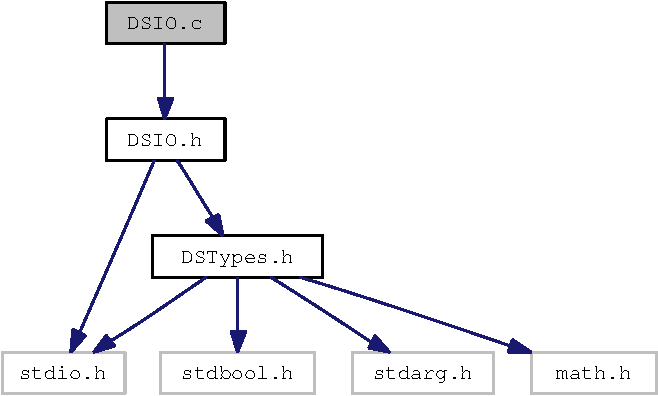
\includegraphics[width=175pt]{_d_s_i_o_8c__incl}
\end{center}
\end{figure}
\subsection*{Defines}
\begin{DoxyCompactItemize}
\item 
\hypertarget{group___d_s___i_o___t_a_g___t_y_p_e_s_gad9110308f40b701fa7a8ac65d48716c6}{
\#define {\bfseries DS\_\-IO\_\-TAG\_\-TYPE\_\-Matrix}~\char`\"{}$\backslash$\char`\"{}\hyperlink{struct_d_s_matrix}{DSMatrix}$\backslash$\char`\"{}\char`\"{}}
\label{group___d_s___i_o___t_a_g___t_y_p_e_s_gad9110308f40b701fa7a8ac65d48716c6}

\item 
\hypertarget{group___d_s___i_o___t_a_g___t_y_p_e_s_ga26f0a22ebdc3e22f453d06fe231c3477}{
\#define {\bfseries DS\_\-IO\_\-TAG\_\-TYPE\_\-MatrixArray}~\char`\"{}$\backslash$\char`\"{}\hyperlink{struct_d_s_matrix_array}{DSMatrixArray}$\backslash$\char`\"{}\char`\"{}}
\label{group___d_s___i_o___t_a_g___t_y_p_e_s_ga26f0a22ebdc3e22f453d06fe231c3477}

\item 
\hypertarget{group___d_s___i_o___t_a_g___t_y_p_e_s_ga33b8d327f394e774d81e2702d27673ec}{
\#define {\bfseries DS\_\-IO\_\-TAG\_\-TYPE\_\-VariablePool}~\char`\"{}$\backslash$\char`\"{}\hyperlink{struct_d_s_variable_pool}{DSVariablePool}$\backslash$\char`\"{}\char`\"{}}
\label{group___d_s___i_o___t_a_g___t_y_p_e_s_ga33b8d327f394e774d81e2702d27673ec}

\item 
\hypertarget{group___d_s___i_o___t_a_g___t_y_p_e_s_ga48168f56a3bd807c4f677f50236f3fd9}{
\#define {\bfseries DS\_\-IO\_\-TAG\_\-TYPE\_\-Dictionary}~\char`\"{}$\backslash$\char`\"{}\hyperlink{struct_d_s_dictionary}{DSDictionary}$\backslash$\char`\"{}\char`\"{}}
\label{group___d_s___i_o___t_a_g___t_y_p_e_s_ga48168f56a3bd807c4f677f50236f3fd9}

\item 
\hypertarget{group___d_s___i_o___t_a_g___t_y_p_e_s_ga9e91e3c5dab3046aa518bf339e1f13e0}{
\#define {\bfseries DS\_\-IO\_\-TAG\_\-TYPE\_\-SSystem}~\char`\"{}$\backslash$\char`\"{}\hyperlink{struct_d_s_s_system}{DSSSystem}$\backslash$\char`\"{}\char`\"{}}
\label{group___d_s___i_o___t_a_g___t_y_p_e_s_ga9e91e3c5dab3046aa518bf339e1f13e0}

\item 
\hypertarget{group___d_s___i_o___t_a_g___t_y_p_e_s_gab40a361af4d08bed8503c9a681f5a51a}{
\#define {\bfseries DS\_\-IO\_\-TAG\_\-TYPE\_\-Case}~\char`\"{}$\backslash$\char`\"{}\hyperlink{struct_d_s_case}{DSCase}$\backslash$\char`\"{}\char`\"{}}
\label{group___d_s___i_o___t_a_g___t_y_p_e_s_gab40a361af4d08bed8503c9a681f5a51a}

\item 
\hypertarget{group___d_s___i_o___t_a_g___t_y_p_e_s_ga4f6f8a8ee7b2387292daf78f6b5fe7ef}{
\#define {\bfseries DS\_\-IO\_\-TAG\_\-TYPE\_\-DesignSpace}~\char`\"{}$\backslash$\char`\"{}\hyperlink{struct_d_s_design_space}{DSDesignSpace}$\backslash$\char`\"{}\char`\"{}}
\label{group___d_s___i_o___t_a_g___t_y_p_e_s_ga4f6f8a8ee7b2387292daf78f6b5fe7ef}

\end{DoxyCompactItemize}
\subsection*{Functions}
\begin{DoxyCompactItemize}
\item 
void \hyperlink{_d_s_i_o_8c_a71e4035e82cf614f1be280b127213ca6}{DSIOSetErrorFile} (FILE $\ast$aFile)
\begin{DoxyCompactList}\small\item\em Function to assign default error file. \item\end{DoxyCompactList}\item 
void \hyperlink{_d_s_i_o_8c_aaa699261767672e938101744e4032249}{DSIOSetPrintFunction} (int($\ast$printFunction)(const char $\ast$,...))
\begin{DoxyCompactList}\small\item\em Function to assign default printf function. \item\end{DoxyCompactList}\item 
void \hyperlink{_d_s_i_o_8c_a37a5183ebd833f0cf9bc2ed19e43fb84}{DSIOSetPostWarningFunction} (void($\ast$warningFunction)(const char $\ast$message))
\begin{DoxyCompactList}\small\item\em Function to assign default warning posting function. \item\end{DoxyCompactList}\item 
void \hyperlink{_d_s_i_o_8c_a8c9be4c3d8b1802aa5295165c3f0b861}{DSIOSetPostErrorFunction} (void($\ast$errorFunction)(const char $\ast$message))
\begin{DoxyCompactList}\small\item\em Function to assign default error posting function. \item\end{DoxyCompactList}\item 
void \hyperlink{_d_s_i_o_8c_a1fbcb57d54a5ac852484b43e317aa43f}{DSIOSetPostFatalErrorFunction} (void($\ast$fatalErrorFunction)(const char $\ast$message))
\begin{DoxyCompactList}\small\item\em Function to assign default fatal error posting function. \item\end{DoxyCompactList}\item 
void \hyperlink{_d_s_i_o_8c_a6cb102dc8b55faa48dca0c51fa0fb517}{DSIOSetCaseJSONOptions} (const DSUInteger options)
\begin{DoxyCompactList}\small\item\em Function that sets the conversion options for a \hyperlink{struct_d_s_case}{DSCase} to JSON format. \item\end{DoxyCompactList}\item 
void \hyperlink{_d_s_i_o_8c_a2a957ad88bd1a2f4d5b0ed616344c7ac}{DSIOSetSSystemJSONOptions} (const DSUInteger options)
\begin{DoxyCompactList}\small\item\em Function that sets the conversion options for a \hyperlink{struct_d_s_s_system}{DSSSystem} to JSON format. \item\end{DoxyCompactList}\item 
char $\ast$ \hyperlink{_d_s_i_o_8c_a754fa75644786b862aabc2660f191d14}{DSVariablePoolStringInJSONFormat} (const \hyperlink{struct_d_s_variable_pool}{DSVariablePool} $\ast$pool)
\begin{DoxyCompactList}\small\item\em Function to convert a \hyperlink{struct_d_s_variable_pool}{DSVariablePool} into a JSON formatted string. \item\end{DoxyCompactList}\item 
char $\ast$ \hyperlink{_d_s_i_o_8c_a6a9e23721286736288947c43461f12ae}{DSMatrixStringInJSONFormat} (const \hyperlink{struct_d_s_matrix}{DSMatrix} $\ast$matrix)
\begin{DoxyCompactList}\small\item\em Function to convert a \hyperlink{struct_d_s_matrix}{DSMatrix} into a JSON formatted string. \item\end{DoxyCompactList}\item 
char $\ast$ \hyperlink{_d_s_i_o_8c_ab8cae51e1c113fc52e1da34fffdc6f40}{DSMatrixArrayStringInJSONFormat} (const \hyperlink{struct_d_s_matrix_array}{DSMatrixArray} $\ast$array)
\begin{DoxyCompactList}\small\item\em Function to convert a \hyperlink{struct_d_s_matrix_array}{DSMatrixArray} into a JSON formatted string. \item\end{DoxyCompactList}\item 
char $\ast$ \hyperlink{_d_s_i_o_8c_a2679d81ab81c12c930cbb7a5e2791d73}{DSSSystemStringInJSONFormat} (const \hyperlink{struct_d_s_s_system}{DSSSystem} $\ast$ssys)
\begin{DoxyCompactList}\small\item\em Function to convert a \hyperlink{struct_d_s_s_system}{DSSSystem} into a JSON formatted string. \item\end{DoxyCompactList}\item 
char $\ast$ \hyperlink{_d_s_i_o_8c_a08dbac8a5ae623c94cf44bd620e46060}{DSCaseStringInJSONFormat} (const \hyperlink{struct_d_s_case}{DSCase} $\ast$aCase)
\begin{DoxyCompactList}\small\item\em Function to convert a \hyperlink{struct_d_s_case}{DSCase} into a JSON formatted string. \item\end{DoxyCompactList}\end{DoxyCompactItemize}
\subsection*{Variables}
\begin{DoxyCompactItemize}
\item 
int($\ast$ \hyperlink{_d_s_i_o_8c_a01ab8215975bf8e2086ad342cfa6be26}{DSPrintf} )(const char $\ast$,...)
\begin{DoxyCompactList}\small\item\em Pointer to a function determining how messages are printed. \item\end{DoxyCompactList}\item 
void($\ast$ \hyperlink{_d_s_i_o_8c_af12cf032b729ba022698fadaccfea33d}{DSPostWarning} )(const char $\ast$message)
\begin{DoxyCompactList}\small\item\em Pointer to a function determining how warning are handled. \item\end{DoxyCompactList}\item 
void($\ast$ \hyperlink{_d_s_i_o_8c_a40c3f80fe9e5002beb7d258e4f89c8d2}{DSPostError} )(const char $\ast$message)
\begin{DoxyCompactList}\small\item\em Pointer to a function determining how errors are handled. \item\end{DoxyCompactList}\item 
void($\ast$ \hyperlink{_d_s_i_o_8c_a41b7b42028f3c25f17ca479154c7492d}{DSPostFatalError} )(const char $\ast$message)
\begin{DoxyCompactList}\small\item\em Pointer to a function determining how fatal errors are handled. \item\end{DoxyCompactList}\item 
FILE $\ast$ \hyperlink{_d_s_i_o_8c_af8405bae84409f99d5fa564ebaff4c91}{DSIOErrorFile}
\begin{DoxyCompactList}\small\item\em FILE pointer used for default error/warning printing. \item\end{DoxyCompactList}\item 
DSUInteger \hyperlink{_d_s_i_o_8c_a54a8bab51a88d9b670634fbe6174c865}{DSSSystemPrintingOptions}
\begin{DoxyCompactList}\small\item\em Variable with flags controlling S-\/System to JSON string conversion. \item\end{DoxyCompactList}\item 
DSUInteger \hyperlink{_d_s_i_o_8c_a3d4acaf78ffb997163a7705876c1feb1}{DSCasePrintingOptions}
\begin{DoxyCompactList}\small\item\em Variable with flags controlling the conversion of a Case to a JSON string. \item\end{DoxyCompactList}\end{DoxyCompactItemize}


\subsection{Detailed Description}
Implementation file with standard input and output functions. Copyright (C) 2011 Jason Lomnitz.

This file is part of the Design Space Toolbox V2 (C Library).

The Design Space Toolbox V2 is free software: you can redistribute it and/or modify it under the terms of the GNU General Public License as published by the Free Software Foundation, either version 3 of the License, or (at your option) any later version.

The Design Space Toolbox V2 is distributed in the hope that it will be useful, but WITHOUT ANY WARRANTY; without even the implied warranty of MERCHANTABILITY or FITNESS FOR A PARTICULAR PURPOSE. See the GNU General Public License for more details.

You should have received a copy of the GNU General Public License along with the Design Space Toolbox. If not, see $<$\href{http://www.gnu.org/licenses/}{\tt http://www.gnu.org/licenses/}$>$.

\begin{DoxyAuthor}{Author}
Jason Lomnitz. 
\end{DoxyAuthor}
\begin{DoxyDate}{Date}
2011 
\end{DoxyDate}


\subsection{Function Documentation}
\hypertarget{_d_s_i_o_8c_a08dbac8a5ae623c94cf44bd620e46060}{
\index{DSIO.c@{DSIO.c}!DSCaseStringInJSONFormat@{DSCaseStringInJSONFormat}}
\index{DSCaseStringInJSONFormat@{DSCaseStringInJSONFormat}!DSIO.c@{DSIO.c}}
\subsubsection[{DSCaseStringInJSONFormat}]{\setlength{\rightskip}{0pt plus 5cm}char$\ast$ DSCaseStringInJSONFormat (const {\bf DSCase} $\ast$ {\em aCase})}}
\label{_d_s_i_o_8c_a08dbac8a5ae623c94cf44bd620e46060}


Function to convert a \hyperlink{struct_d_s_case}{DSCase} into a JSON formatted string. 

This function is used to convert a \hyperlink{struct_d_s_case}{DSCase} into a JSON object. The \hyperlink{struct_d_s_case}{DSCase} is represented with a set of objects, where each object is a field of the \hyperlink{struct_d_s_case}{DSCase} object. The default behavior exports all of the fields, this behavior can be overwritten by changing the \hyperlink{struct_d_s_case}{DSCase} conversion options.


\begin{DoxyParams}{Parameters}
\item[{\em aCase}]A \hyperlink{struct_d_s_case}{DSCase} that will be used to create the JSON object.\end{DoxyParams}
\begin{DoxyReturn}{Returns}
A C string with the JSON formatted data. If NULL, the conversion failed.
\end{DoxyReturn}
\begin{DoxySeeAlso}{See also}
\hyperlink{_d_s_i_o_8c_a6cb102dc8b55faa48dca0c51fa0fb517}{DSIOSetCaseJSONOptions()} 
\end{DoxySeeAlso}
\hypertarget{_d_s_i_o_8c_a6cb102dc8b55faa48dca0c51fa0fb517}{
\index{DSIO.c@{DSIO.c}!DSIOSetCaseJSONOptions@{DSIOSetCaseJSONOptions}}
\index{DSIOSetCaseJSONOptions@{DSIOSetCaseJSONOptions}!DSIO.c@{DSIO.c}}
\subsubsection[{DSIOSetCaseJSONOptions}]{\setlength{\rightskip}{0pt plus 5cm}void DSIOSetCaseJSONOptions (const DSUInteger {\em options})}}
\label{_d_s_i_o_8c_a6cb102dc8b55faa48dca0c51fa0fb517}


Function that sets the conversion options for a \hyperlink{struct_d_s_case}{DSCase} to JSON format. 

This function is used to overwrite the default export behavior of the \hyperlink{struct_d_s_case}{DSCase} object. The default behavior converts all of the data fields of the \hyperlink{struct_d_s_case}{DSCase} into a JSON format, these options can be changed so the JSON conversion only includes some fields, such as excluding the conditions, excluding the S-\/System, etc.


\begin{DoxyParams}{Parameters}
\item[{\em options}]A DSUInteger with the option flags, as specified by the \hyperlink{struct_d_s_case}{DSCase} options.\end{DoxyParams}
\begin{DoxySeeAlso}{See also}
\hyperlink{group___d_s___c_a_s_e___j_s_o_n___o_p_t_i_o_n_s}{Options for JSON conversion of DSCase object.} 
\end{DoxySeeAlso}
\hypertarget{_d_s_i_o_8c_a71e4035e82cf614f1be280b127213ca6}{
\index{DSIO.c@{DSIO.c}!DSIOSetErrorFile@{DSIOSetErrorFile}}
\index{DSIOSetErrorFile@{DSIOSetErrorFile}!DSIO.c@{DSIO.c}}
\subsubsection[{DSIOSetErrorFile}]{\setlength{\rightskip}{0pt plus 5cm}void DSIOSetErrorFile (FILE $\ast$ {\em aFile})}}
\label{_d_s_i_o_8c_a71e4035e82cf614f1be280b127213ca6}


Function to assign default error file. 

This function is used to assign the default error file, DSIOErrorFile. Changing the error file should be done via this function, as it circumvents potential problems associated with dynamic linking.


\begin{DoxyParams}{Parameters}
\item[{\em aFile}]A FILE $\ast$ that will be used to write error messages when the default error posting mechanism is used.\end{DoxyParams}
\begin{DoxySeeAlso}{See also}
\hyperlink{_d_s_i_o_8h_a37a5183ebd833f0cf9bc2ed19e43fb84}{DSIOSetPostWarningFunction} 

\hyperlink{_d_s_i_o_8h_a8c9be4c3d8b1802aa5295165c3f0b861}{DSIOSetPostErrorFunction} 

\hyperlink{_d_s_i_o_8h_a1fbcb57d54a5ac852484b43e317aa43f}{DSIOSetPostFatalErrorFunction} 

\hyperlink{_d_s_errors_8h_a09b28eb2b01986855910ca97dfe91144}{DSError} 
\end{DoxySeeAlso}
\hypertarget{_d_s_i_o_8c_a8c9be4c3d8b1802aa5295165c3f0b861}{
\index{DSIO.c@{DSIO.c}!DSIOSetPostErrorFunction@{DSIOSetPostErrorFunction}}
\index{DSIOSetPostErrorFunction@{DSIOSetPostErrorFunction}!DSIO.c@{DSIO.c}}
\subsubsection[{DSIOSetPostErrorFunction}]{\setlength{\rightskip}{0pt plus 5cm}void DSIOSetPostErrorFunction (void($\ast$)(const char $\ast$message) {\em errorFunction})}}
\label{_d_s_i_o_8c_a8c9be4c3d8b1802aa5295165c3f0b861}


Function to assign default error posting function. 

This function is used to assign the function that handles the errors generated from the design space toolbox. Internally, it assigns the global variable DSPostError which points to a function.


\begin{DoxyParams}{Parameters}
\item[{\em errorFunction}]A pointer to a function of the form void function(const char $\ast$). If NULL, default behavior is restored. \end{DoxyParams}
\hypertarget{_d_s_i_o_8c_a1fbcb57d54a5ac852484b43e317aa43f}{
\index{DSIO.c@{DSIO.c}!DSIOSetPostFatalErrorFunction@{DSIOSetPostFatalErrorFunction}}
\index{DSIOSetPostFatalErrorFunction@{DSIOSetPostFatalErrorFunction}!DSIO.c@{DSIO.c}}
\subsubsection[{DSIOSetPostFatalErrorFunction}]{\setlength{\rightskip}{0pt plus 5cm}void DSIOSetPostFatalErrorFunction (void($\ast$)(const char $\ast$message) {\em fatalErrorFunction})}}
\label{_d_s_i_o_8c_a1fbcb57d54a5ac852484b43e317aa43f}


Function to assign default fatal error posting function. 

This function is used to assign the function that handles the fatal errors generated from the design space toolbox. Internally, it assigns the global variable DSPostFatalError which points to a function.


\begin{DoxyParams}{Parameters}
\item[{\em errorFunction}]A pointer to a function of the form void function(const char $\ast$). If NULL, default behavior is restored. \end{DoxyParams}
\hypertarget{_d_s_i_o_8c_a37a5183ebd833f0cf9bc2ed19e43fb84}{
\index{DSIO.c@{DSIO.c}!DSIOSetPostWarningFunction@{DSIOSetPostWarningFunction}}
\index{DSIOSetPostWarningFunction@{DSIOSetPostWarningFunction}!DSIO.c@{DSIO.c}}
\subsubsection[{DSIOSetPostWarningFunction}]{\setlength{\rightskip}{0pt plus 5cm}void DSIOSetPostWarningFunction (void($\ast$)(const char $\ast$message) {\em warningFunction})}}
\label{_d_s_i_o_8c_a37a5183ebd833f0cf9bc2ed19e43fb84}


Function to assign default warning posting function. 

This function is used to assign the function that handles the warnings generated from the design space toolbox. Internally, it assigns the global variable DSPostWarning which points to a function.


\begin{DoxyParams}{Parameters}
\item[{\em warningFunction}]A pointer to a function of the form void function(const char $\ast$). If NULL, default behavior is restored. \end{DoxyParams}
\hypertarget{_d_s_i_o_8c_aaa699261767672e938101744e4032249}{
\index{DSIO.c@{DSIO.c}!DSIOSetPrintFunction@{DSIOSetPrintFunction}}
\index{DSIOSetPrintFunction@{DSIOSetPrintFunction}!DSIO.c@{DSIO.c}}
\subsubsection[{DSIOSetPrintFunction}]{\setlength{\rightskip}{0pt plus 5cm}void DSIOSetPrintFunction (int($\ast$)(const char $\ast$,...) {\em printFunction})}}
\label{_d_s_i_o_8c_aaa699261767672e938101744e4032249}


Function to assign default printf function. 

This function is used to assign the formated print function, DSPrintf. This function assigns the DSPrintf pointer to the function that should be used to print formatted strings. This function MUST be used to avoid problems relating to dynamic linking; by using this function the global variable DSPrintf is loaded into memory prior to changing its value.


\begin{DoxyParams}{Parameters}
\item[{\em printFunction}]A pointer to a function of the form int function(const char $\ast$, ...). If NULL, default behavior is restored. \end{DoxyParams}
\hypertarget{_d_s_i_o_8c_a2a957ad88bd1a2f4d5b0ed616344c7ac}{
\index{DSIO.c@{DSIO.c}!DSIOSetSSystemJSONOptions@{DSIOSetSSystemJSONOptions}}
\index{DSIOSetSSystemJSONOptions@{DSIOSetSSystemJSONOptions}!DSIO.c@{DSIO.c}}
\subsubsection[{DSIOSetSSystemJSONOptions}]{\setlength{\rightskip}{0pt plus 5cm}void DSIOSetSSystemJSONOptions (const DSUInteger {\em options})}}
\label{_d_s_i_o_8c_a2a957ad88bd1a2f4d5b0ed616344c7ac}


Function that sets the conversion options for a \hyperlink{struct_d_s_s_system}{DSSSystem} to JSON format. 

This function is used to overwrite the default export behavior of the \hyperlink{struct_d_s_s_system}{DSSSystem} object. The default behavior converts all of the data fields of the S-\/System into a JSON format, these options can be changed so the JSON conversion only includes some fields, such as excluding the solution.


\begin{DoxyParams}{Parameters}
\item[{\em options}]A DSUInteger with the option flags, as specified by the \hyperlink{struct_d_s_s_system}{DSSSystem} options.\end{DoxyParams}
\begin{DoxySeeAlso}{See also}
\hyperlink{group___d_s___s_s_y_s_t_e_m___j_s_o_n___o_p_t_i_o_n_s}{Options for JSON conversion of DSSSystem object.} 
\end{DoxySeeAlso}
\hypertarget{_d_s_i_o_8c_ab8cae51e1c113fc52e1da34fffdc6f40}{
\index{DSIO.c@{DSIO.c}!DSMatrixArrayStringInJSONFormat@{DSMatrixArrayStringInJSONFormat}}
\index{DSMatrixArrayStringInJSONFormat@{DSMatrixArrayStringInJSONFormat}!DSIO.c@{DSIO.c}}
\subsubsection[{DSMatrixArrayStringInJSONFormat}]{\setlength{\rightskip}{0pt plus 5cm}char$\ast$ DSMatrixArrayStringInJSONFormat (const {\bf DSMatrixArray} $\ast$ {\em array})}}
\label{_d_s_i_o_8c_ab8cae51e1c113fc52e1da34fffdc6f40}


Function to convert a \hyperlink{struct_d_s_matrix_array}{DSMatrixArray} into a JSON formatted string. 

This function is used to convert a \hyperlink{struct_d_s_matrix}{DSMatrix} into a JSON object. The matrix array is stored as an array of objects, where each object is a \hyperlink{struct_d_s_matrix}{DSMatrix}. The order of the \hyperlink{struct_d_s_matrix}{DSMatrix} object in the array represent the order of matrices in the matrix array.


\begin{DoxyParams}{Parameters}
\item[{\em array}]A \hyperlink{struct_d_s_matrix_array}{DSMatrixArray} that will be used to create the JSON object.\end{DoxyParams}
\begin{DoxyReturn}{Returns}
A C string with the JSON formatted data. If NULL, the conversion failed. 
\end{DoxyReturn}
\hypertarget{_d_s_i_o_8c_a6a9e23721286736288947c43461f12ae}{
\index{DSIO.c@{DSIO.c}!DSMatrixStringInJSONFormat@{DSMatrixStringInJSONFormat}}
\index{DSMatrixStringInJSONFormat@{DSMatrixStringInJSONFormat}!DSIO.c@{DSIO.c}}
\subsubsection[{DSMatrixStringInJSONFormat}]{\setlength{\rightskip}{0pt plus 5cm}char$\ast$ DSMatrixStringInJSONFormat (const {\bf DSMatrix} $\ast$ {\em matrix})}}
\label{_d_s_i_o_8c_a6a9e23721286736288947c43461f12ae}


Function to convert a \hyperlink{struct_d_s_matrix}{DSMatrix} into a JSON formatted string. 

This function is used to convert a \hyperlink{struct_d_s_matrix}{DSMatrix} into a JSON object. The matrix is stored as an array of arrays. The array of arrays represents the rows of the matrix, whereas the arrays of value are the values at the columns for a particular row.


\begin{DoxyParams}{Parameters}
\item[{\em matrix}]A \hyperlink{struct_d_s_matrix}{DSMatrix} that will be used to create the JSON object.\end{DoxyParams}
\begin{DoxyReturn}{Returns}
A C string with the JSON formatted data. If NULL, the conversion failed. 
\end{DoxyReturn}
\hypertarget{_d_s_i_o_8c_a2679d81ab81c12c930cbb7a5e2791d73}{
\index{DSIO.c@{DSIO.c}!DSSSystemStringInJSONFormat@{DSSSystemStringInJSONFormat}}
\index{DSSSystemStringInJSONFormat@{DSSSystemStringInJSONFormat}!DSIO.c@{DSIO.c}}
\subsubsection[{DSSSystemStringInJSONFormat}]{\setlength{\rightskip}{0pt plus 5cm}char$\ast$ DSSSystemStringInJSONFormat (const {\bf DSSSystem} $\ast$ {\em ssys})}}
\label{_d_s_i_o_8c_a2679d81ab81c12c930cbb7a5e2791d73}


Function to convert a \hyperlink{struct_d_s_s_system}{DSSSystem} into a JSON formatted string. 

This function is used to convert a \hyperlink{struct_d_s_s_system}{DSSSystem} into a JSON object. The S-\/System as a set of objects, where each object represents each of the fields of the \hyperlink{struct_d_s_s_system}{DSSSystem}. The default behavior exports all of the fields, this behavior can be overwritten by changing the S-\/System conversion options.


\begin{DoxyParams}{Parameters}
\item[{\em ssys}]A \hyperlink{struct_d_s_s_system}{DSSSystem} that will be used to create the JSON object.\end{DoxyParams}
\begin{DoxyReturn}{Returns}
A C string with the JSON formatted data. If NULL, the conversion failed.
\end{DoxyReturn}
\begin{DoxySeeAlso}{See also}
\hyperlink{_d_s_i_o_8c_a2a957ad88bd1a2f4d5b0ed616344c7ac}{DSIOSetSSystemJSONOptions()} 
\end{DoxySeeAlso}
\hypertarget{_d_s_i_o_8c_a754fa75644786b862aabc2660f191d14}{
\index{DSIO.c@{DSIO.c}!DSVariablePoolStringInJSONFormat@{DSVariablePoolStringInJSONFormat}}
\index{DSVariablePoolStringInJSONFormat@{DSVariablePoolStringInJSONFormat}!DSIO.c@{DSIO.c}}
\subsubsection[{DSVariablePoolStringInJSONFormat}]{\setlength{\rightskip}{0pt plus 5cm}char$\ast$ DSVariablePoolStringInJSONFormat (const {\bf DSVariablePool} $\ast$ {\em pool})}}
\label{_d_s_i_o_8c_a754fa75644786b862aabc2660f191d14}


Function to convert a \hyperlink{struct_d_s_variable_pool}{DSVariablePool} into a JSON formatted string. 

This function is used to convert a \hyperlink{struct_d_s_variable_pool}{DSVariablePool} into a JSON object. The variables of the variable pool are stored as pairs of a string and value.


\begin{DoxyParams}{Parameters}
\item[{\em pool}]A \hyperlink{struct_d_s_variable_pool}{DSVariablePool} that will be used to create the JSON object.\end{DoxyParams}
\begin{DoxyReturn}{Returns}
A C string with the JSON formatted data. If NULL, the conversion failed. 
\end{DoxyReturn}


\subsection{Variable Documentation}
\hypertarget{_d_s_i_o_8c_a3d4acaf78ffb997163a7705876c1feb1}{
\index{DSIO.c@{DSIO.c}!DSCasePrintingOptions@{DSCasePrintingOptions}}
\index{DSCasePrintingOptions@{DSCasePrintingOptions}!DSIO.c@{DSIO.c}}
\subsubsection[{DSCasePrintingOptions}]{\setlength{\rightskip}{0pt plus 5cm}DSUInteger {\bf DSCasePrintingOptions}}}
\label{_d_s_i_o_8c_a3d4acaf78ffb997163a7705876c1feb1}


Variable with flags controlling the conversion of a Case to a JSON string. 

This global variable is checked when converting a Case structure to a JSON string. This variable will check several flags as specified by DS\_\-CASE\_\-JSON\_\-OPTIONS. The default value of the variable indicates that all the properties will be included in the JSON string.

\begin{DoxySeeAlso}{See also}
\hyperlink{group___d_s___c_a_s_e___j_s_o_n___o_p_t_i_o_n_s}{Options for JSON conversion of DSCase object.} 

\hyperlink{_d_s_i_o_8c_a6cb102dc8b55faa48dca0c51fa0fb517}{DSIOSetCaseJSONOptions()} 
\end{DoxySeeAlso}
\hypertarget{_d_s_i_o_8c_af8405bae84409f99d5fa564ebaff4c91}{
\index{DSIO.c@{DSIO.c}!DSIOErrorFile@{DSIOErrorFile}}
\index{DSIOErrorFile@{DSIOErrorFile}!DSIO.c@{DSIO.c}}
\subsubsection[{DSIOErrorFile}]{\setlength{\rightskip}{0pt plus 5cm}FILE$\ast$ {\bf DSIOErrorFile}}}
\label{_d_s_i_o_8c_af8405bae84409f99d5fa564ebaff4c91}


FILE pointer used for default error/warning printing. 

This pointer to a FILE tells the error handling system which FILE to print the error messages to. If this pointer is NULL, then the system sets it to the stderr file. This variable is only used internally with the default behavior of DSErrorFunction. To change the error file, the function DSIOSetErrorFile should be used in order to avoid errors caused by dynamic linking. These errors involve changing the value of a global variable that has not yet been loaded by the linker.

\begin{DoxySeeAlso}{See also}
\hyperlink{_d_s_i_o_8h_a71e4035e82cf614f1be280b127213ca6}{DSIOSetErrorFile} 

\hyperlink{_d_s_errors_8h_a363f9c264b785ec509da1b11af9ae314}{DSErrorFunction} 
\end{DoxySeeAlso}
\hypertarget{_d_s_i_o_8c_a40c3f80fe9e5002beb7d258e4f89c8d2}{
\index{DSIO.c@{DSIO.c}!DSPostError@{DSPostError}}
\index{DSPostError@{DSPostError}!DSIO.c@{DSIO.c}}
\subsubsection[{DSPostError}]{\setlength{\rightskip}{0pt plus 5cm}void($\ast$ {\bf DSPostError})(const char $\ast$message)}}
\label{_d_s_i_o_8c_a40c3f80fe9e5002beb7d258e4f89c8d2}


Pointer to a function determining how errors are handled. 

This pointer to a function is used by DSErrorFunction to post erros. This pointer should be used to allow better integration of errors in programs that make use of the DesignSpaceToolbox. The function takes one argument, a constant C string with the error message. To change the function used, the function DSIOSetPostErrorFunction should be used. This is to avoid errors caused by dynamic linking. These errors involve changing the value of a global variable that has not yet been loaded by the linker.

\begin{DoxySeeAlso}{See also}
\hyperlink{_d_s_i_o_8h_a8c9be4c3d8b1802aa5295165c3f0b861}{DSIOSetPostErrorFunction} 
\end{DoxySeeAlso}
\hypertarget{_d_s_i_o_8c_a41b7b42028f3c25f17ca479154c7492d}{
\index{DSIO.c@{DSIO.c}!DSPostFatalError@{DSPostFatalError}}
\index{DSPostFatalError@{DSPostFatalError}!DSIO.c@{DSIO.c}}
\subsubsection[{DSPostFatalError}]{\setlength{\rightskip}{0pt plus 5cm}void($\ast$ {\bf DSPostFatalError})(const char $\ast$message)}}
\label{_d_s_i_o_8c_a41b7b42028f3c25f17ca479154c7492d}


Pointer to a function determining how fatal errors are handled. 

This pointer to a function is used by DSErrorFunction to post fatal erros. This pointer should be used to allow better integration of errors in programs that make use of the DesignSpaceToolbox. The function takes one argument, a constant C string with the error message. To change the function used, the function DSIOSetPostFatalErrorFunction should be used. This is to avoid errors caused by dynamic linking. These errors involve changing the value of a global variable that has not yet been loaded by the linker.

\begin{DoxySeeAlso}{See also}
\hyperlink{_d_s_i_o_8h_a8c9be4c3d8b1802aa5295165c3f0b861}{DSIOSetPostErrorFunction} 
\end{DoxySeeAlso}
\hypertarget{_d_s_i_o_8c_af12cf032b729ba022698fadaccfea33d}{
\index{DSIO.c@{DSIO.c}!DSPostWarning@{DSPostWarning}}
\index{DSPostWarning@{DSPostWarning}!DSIO.c@{DSIO.c}}
\subsubsection[{DSPostWarning}]{\setlength{\rightskip}{0pt plus 5cm}void($\ast$ {\bf DSPostWarning})(const char $\ast$message)}}
\label{_d_s_i_o_8c_af12cf032b729ba022698fadaccfea33d}


Pointer to a function determining how warning are handled. 

This pointer to a function is used by DSErrorFunction to post warnings. This pointer should be used to allow better integration of warnings in programs that make use of the DesignSpaceToolbox. The function takes one argument, a constant C string with the warning message. To change the function used, the function DSIOSetPostWarningFunction should be used. This is to avoid errors caused by dynamic linking. These errors involve changing the value of a global variable that has not yet been loaded by the linker.

\begin{DoxySeeAlso}{See also}
\hyperlink{_d_s_i_o_8h_a37a5183ebd833f0cf9bc2ed19e43fb84}{DSIOSetPostWarningFunction} 
\end{DoxySeeAlso}
\hypertarget{_d_s_i_o_8c_a01ab8215975bf8e2086ad342cfa6be26}{
\index{DSIO.c@{DSIO.c}!DSPrintf@{DSPrintf}}
\index{DSPrintf@{DSPrintf}!DSIO.c@{DSIO.c}}
\subsubsection[{DSPrintf}]{\setlength{\rightskip}{0pt plus 5cm}int($\ast$ {\bf DSPrintf})(const char $\ast$,...)}}
\label{_d_s_i_o_8c_a01ab8215975bf8e2086ad342cfa6be26}


Pointer to a function determining how messages are printed. 

This pointer to a function tells the error handling system which function to call with the error messages. If this pointer is NULL, the design space toolbox should have a default printing format, using printf to stdout. This pointer is intended to be used to override default behavior to be override. An example could be by using the mexPrintf function in matlab.

\begin{DoxySeeAlso}{See also}
\hyperlink{_d_s_i_o_8h_aaa699261767672e938101744e4032249}{DSIOSetPrintFunction} 
\end{DoxySeeAlso}
\hypertarget{_d_s_i_o_8c_a54a8bab51a88d9b670634fbe6174c865}{
\index{DSIO.c@{DSIO.c}!DSSSystemPrintingOptions@{DSSSystemPrintingOptions}}
\index{DSSSystemPrintingOptions@{DSSSystemPrintingOptions}!DSIO.c@{DSIO.c}}
\subsubsection[{DSSSystemPrintingOptions}]{\setlength{\rightskip}{0pt plus 5cm}DSUInteger {\bf DSSSystemPrintingOptions}}}
\label{_d_s_i_o_8c_a54a8bab51a88d9b670634fbe6174c865}


Variable with flags controlling S-\/System to JSON string conversion. 

This global variable is checked when converting a S-\/System structure to a JSON string. This variable will check several flags as specified by DS\_\-SSYSTEM\_\-JSON\_\-OPTIONS. The default value of the variable indicates that all the properties will be included in the JSON string.

\begin{DoxySeeAlso}{See also}
\hyperlink{group___d_s___s_s_y_s_t_e_m___j_s_o_n___o_p_t_i_o_n_s}{Options for JSON conversion of DSSSystem object.} 

\hyperlink{_d_s_i_o_8c_a2a957ad88bd1a2f4d5b0ed616344c7ac}{DSIOSetSSystemJSONOptions()} 
\end{DoxySeeAlso}

\hypertarget{_d_s_i_o_8h}{
\section{DSIO.h File Reference}
\label{_d_s_i_o_8h}\index{DSIO.h@{DSIO.h}}
}


Header file with standard input and output functions.  


{\ttfamily \#include $<$stdio.h$>$}\par
{\ttfamily \#include \char`\"{}DSTypes.h\char`\"{}}\par
Include dependency graph for DSIO.h:\nopagebreak
\begin{figure}[H]
\begin{center}
\leavevmode
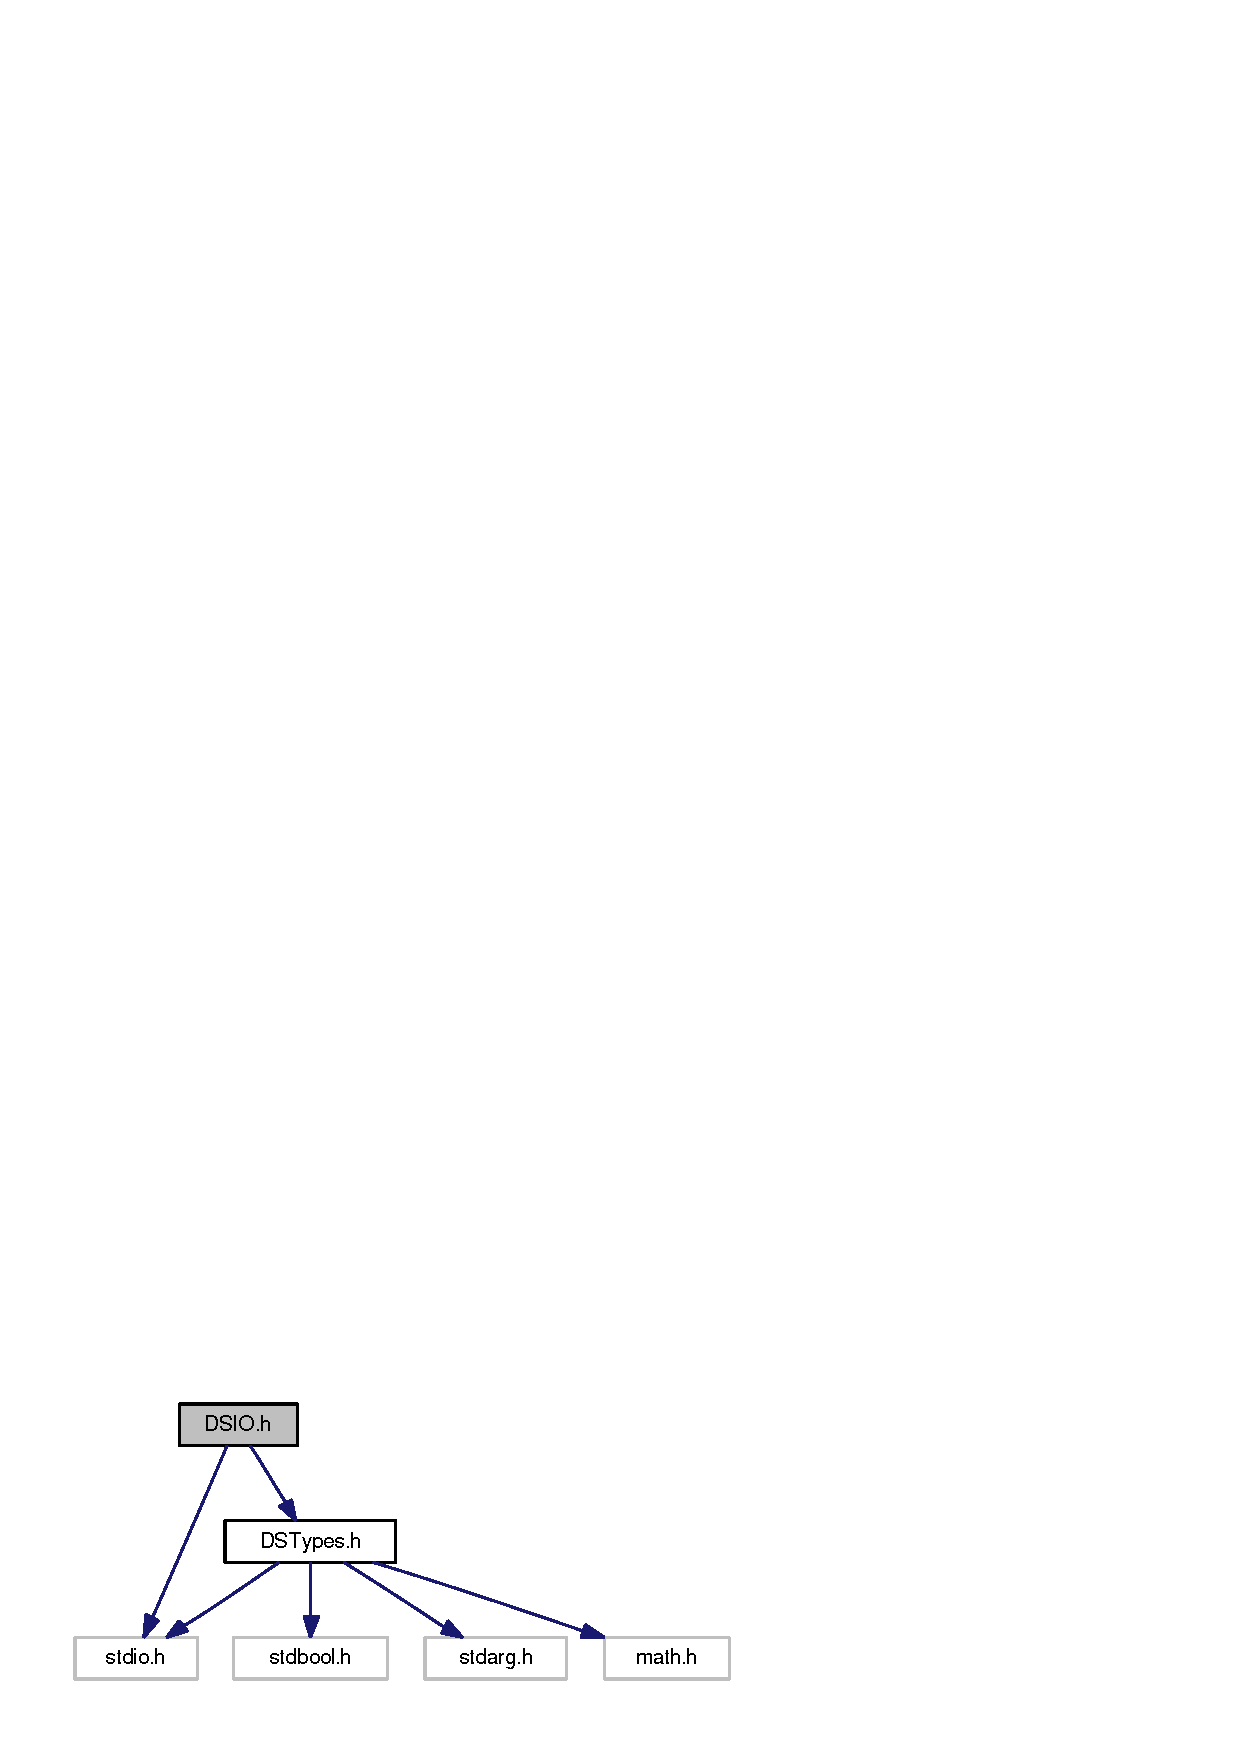
\includegraphics[width=175pt]{_d_s_i_o_8h__incl}
\end{center}
\end{figure}
This graph shows which files directly or indirectly include this file:\nopagebreak
\begin{figure}[H]
\begin{center}
\leavevmode
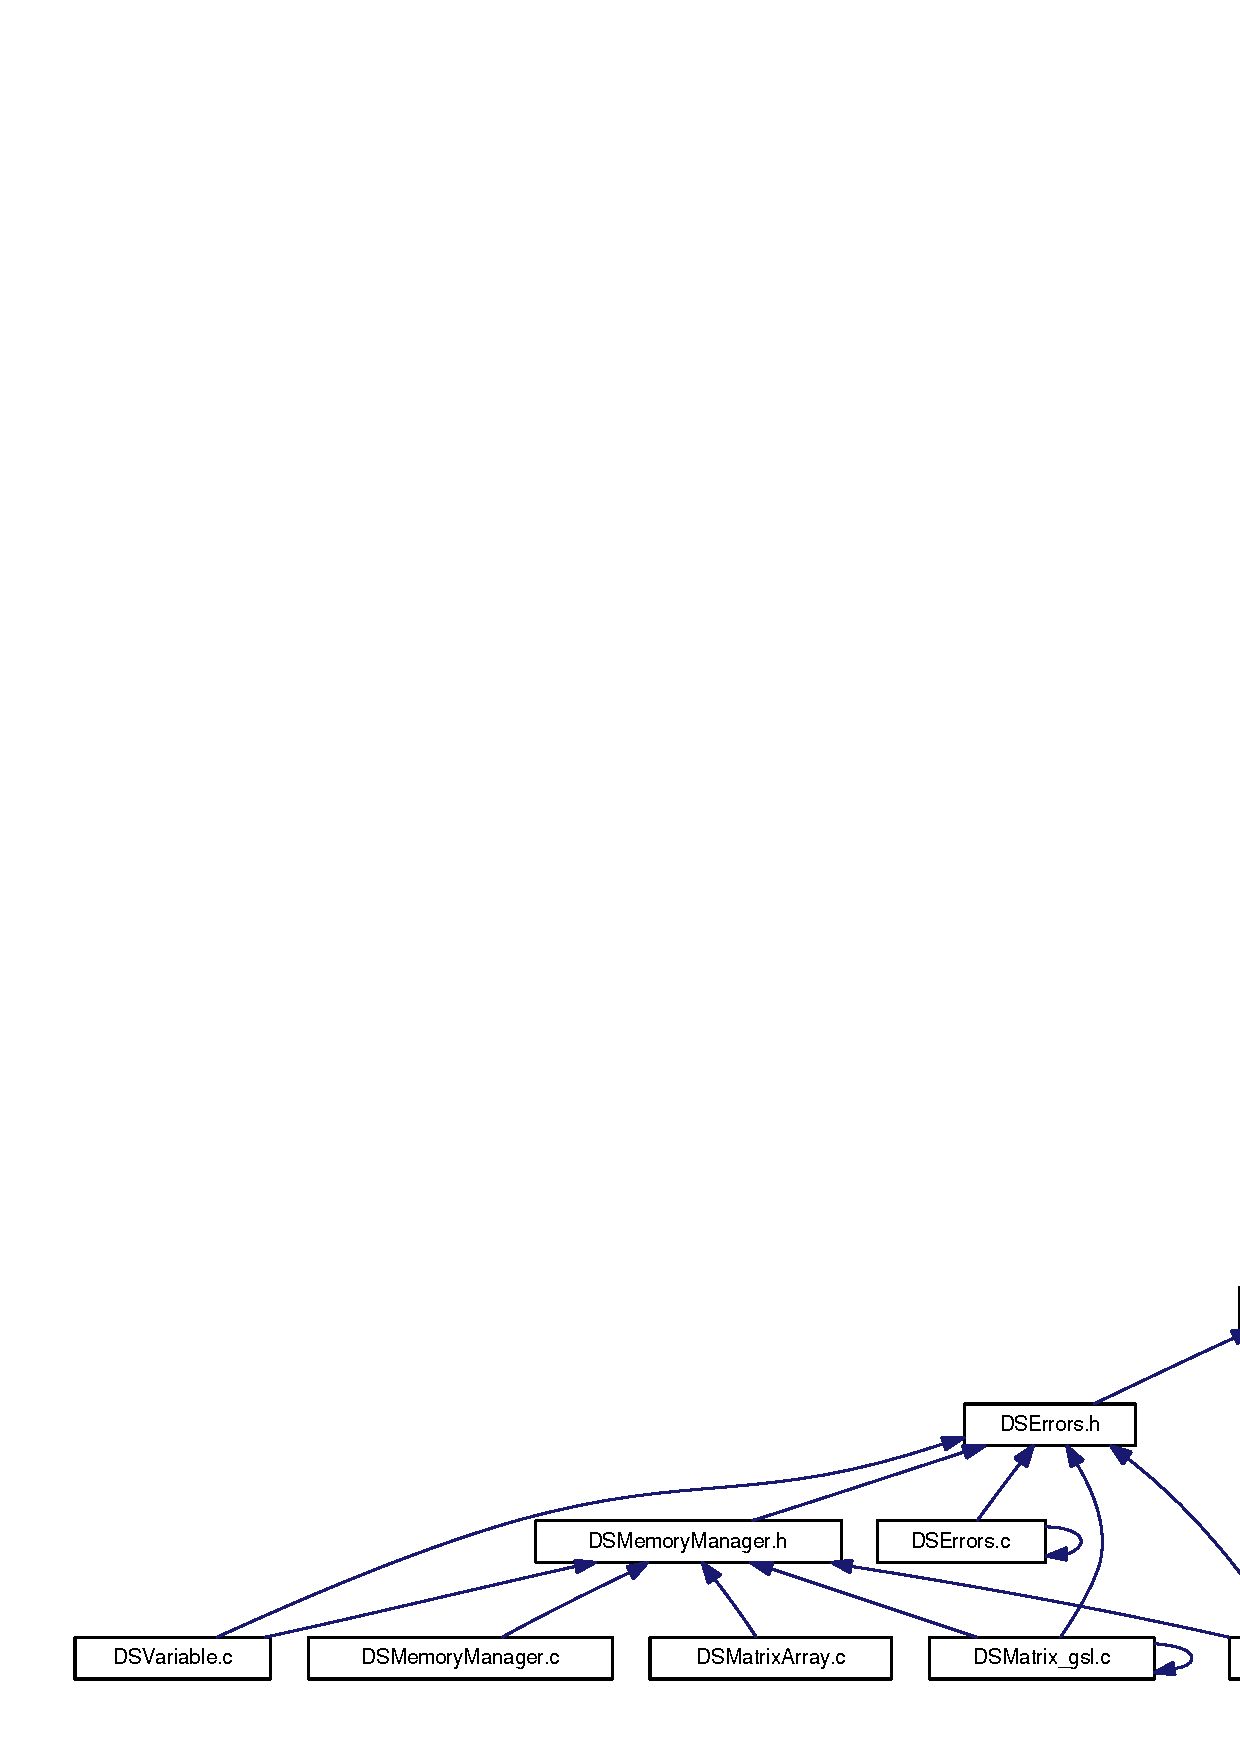
\includegraphics[width=354pt]{_d_s_i_o_8h__dep__incl}
\end{center}
\end{figure}
\subsection*{Functions}
\begin{DoxyCompactItemize}
\item 
void \hyperlink{_d_s_i_o_8h_a71e4035e82cf614f1be280b127213ca6}{DSIOSetErrorFile} (FILE $\ast$aFile)
\begin{DoxyCompactList}\small\item\em Function to assign default error file. \item\end{DoxyCompactList}\item 
\hypertarget{_d_s_i_o_8h_aaa699261767672e938101744e4032249}{
void {\bfseries DSIOSetPrintFunction} (int($\ast$printFunction)(const char $\ast$,...))}
\label{_d_s_i_o_8h_aaa699261767672e938101744e4032249}

\item 
\hypertarget{_d_s_i_o_8h_a37a5183ebd833f0cf9bc2ed19e43fb84}{
void {\bfseries DSIOSetPostWarningFunction} (void($\ast$warningFunction)(const char $\ast$message))}
\label{_d_s_i_o_8h_a37a5183ebd833f0cf9bc2ed19e43fb84}

\item 
\hypertarget{_d_s_i_o_8h_a8c9be4c3d8b1802aa5295165c3f0b861}{
void {\bfseries DSIOSetPostErrorFunction} (void($\ast$errorFunction)(const char $\ast$message))}
\label{_d_s_i_o_8h_a8c9be4c3d8b1802aa5295165c3f0b861}

\item 
\hypertarget{_d_s_i_o_8h_a1fbcb57d54a5ac852484b43e317aa43f}{
void {\bfseries DSIOSetPostFatalErrorFunction} (void($\ast$fatalErrorFunction)(const char $\ast$message))}
\label{_d_s_i_o_8h_a1fbcb57d54a5ac852484b43e317aa43f}

\end{DoxyCompactItemize}
\subsection*{Variables}
\begin{DoxyCompactItemize}
\item 
int($\ast$ \hyperlink{_d_s_i_o_8h_a01ab8215975bf8e2086ad342cfa6be26}{DSPrintf} )(const char $\ast$,...)
\begin{DoxyCompactList}\small\item\em Pointer to a function determining how messages are printed. \item\end{DoxyCompactList}\item 
\hypertarget{_d_s_i_o_8h_af12cf032b729ba022698fadaccfea33d}{
void($\ast$ {\bfseries DSPostWarning} )(const char $\ast$message)}
\label{_d_s_i_o_8h_af12cf032b729ba022698fadaccfea33d}

\item 
\hypertarget{_d_s_i_o_8h_a40c3f80fe9e5002beb7d258e4f89c8d2}{
void($\ast$ {\bfseries DSPostError} )(const char $\ast$message)}
\label{_d_s_i_o_8h_a40c3f80fe9e5002beb7d258e4f89c8d2}

\item 
\hypertarget{_d_s_i_o_8h_a41b7b42028f3c25f17ca479154c7492d}{
void($\ast$ {\bfseries DSPostFatalError} )(const char $\ast$message)}
\label{_d_s_i_o_8h_a41b7b42028f3c25f17ca479154c7492d}

\item 
\hypertarget{_d_s_i_o_8h_af8405bae84409f99d5fa564ebaff4c91}{
FILE $\ast$ {\bfseries DSIOErrorFile}}
\label{_d_s_i_o_8h_af8405bae84409f99d5fa564ebaff4c91}

\end{DoxyCompactItemize}


\subsection{Detailed Description}
Header file with standard input and output functions. Copyright (C) 2011 Jason Lomnitz.\par
\par


This file is part of the Design Space Toolbox V2 (C Library).

The Design Space Toolbox V2 is free software: you can redistribute it and/or modify it under the terms of the GNU General Public License as published by the Free Software Foundation, either version 3 of the License, or (at your option) any later version.

The Design Space Toolbox V2 is distributed in the hope that it will be useful, but WITHOUT ANY WARRANTY; without even the implied warranty of MERCHANTABILITY or FITNESS FOR A PARTICULAR PURPOSE. See the GNU General Public License for more details.

You should have received a copy of the GNU General Public License along with the Design Space Toolbox. If not, see $<$\href{http://www.gnu.org/licenses/}{\tt http://www.gnu.org/licenses/}$>$.

\begin{DoxyAuthor}{Author}
Jason Lomnitz. 
\end{DoxyAuthor}
\begin{DoxyDate}{Date}
2011
\end{DoxyDate}
\begin{Desc}
\item[\hyperlink{todo__todo000001}{Todo}]Add 'plug-\/in' for printf function. 

Define standard input and output file formats.\end{Desc}


\subsection{Function Documentation}
\hypertarget{_d_s_i_o_8h_a71e4035e82cf614f1be280b127213ca6}{
\index{DSIO.h@{DSIO.h}!DSIOSetErrorFile@{DSIOSetErrorFile}}
\index{DSIOSetErrorFile@{DSIOSetErrorFile}!DSIO.h@{DSIO.h}}
\subsubsection[{DSIOSetErrorFile}]{\setlength{\rightskip}{0pt plus 5cm}void DSIOSetErrorFile (FILE $\ast$ {\em aFile})}}
\label{_d_s_i_o_8h_a71e4035e82cf614f1be280b127213ca6}


Function to assign default error file. 

This function is used to assign the default error file, DSIOErrorFile. Changing the error file should be done via this function, as it circumvents potential problems associated with dynamic linking.


\begin{DoxyParams}{Parameters}
\item[{\em aFile}]A FILE $\ast$ that will be used to write error messages when the default error posting mechanism is used.\end{DoxyParams}
\begin{DoxySeeAlso}{See also}
DSIOSetPostWarningFunction 

DSIOSetPostErrorFunction 

DSIOSetPostFatalErrorFunction 

\hyperlink{_d_s_errors_8h_a09b28eb2b01986855910ca97dfe91144}{DSError} 
\end{DoxySeeAlso}


\subsection{Variable Documentation}
\hypertarget{_d_s_i_o_8h_a01ab8215975bf8e2086ad342cfa6be26}{
\index{DSIO.h@{DSIO.h}!DSPrintf@{DSPrintf}}
\index{DSPrintf@{DSPrintf}!DSIO.h@{DSIO.h}}
\subsubsection[{DSPrintf}]{\setlength{\rightskip}{0pt plus 5cm}int($\ast$ {\bf DSPrintf})(const char $\ast$,...)}}
\label{_d_s_i_o_8h_a01ab8215975bf8e2086ad342cfa6be26}


Pointer to a function determining how messages are printed. 

This pointer to a function tells the error handling system which function to call with the error messages. If this pointer is NULL, the design space toolbox should have a default printing format, using printf to stdout. This pointer is intended to be used to override default behavior to be override. An example could be by using the mexPrintf function in matlab.

\begin{DoxySeeAlso}{See also}
DSIOSetPrintFunction 
\end{DoxySeeAlso}

\hypertarget{_d_s_matrix_8h}{
\section{DSMatrix.h File Reference}
\label{_d_s_matrix_8h}\index{DSMatrix.h@{DSMatrix.h}}
}


Header file with functions for dealing with matrices.  


{\ttfamily \#include \char`\"{}DSTypes.h\char`\"{}}\par
Include dependency graph for DSMatrix.h:\nopagebreak
\begin{figure}[H]
\begin{center}
\leavevmode
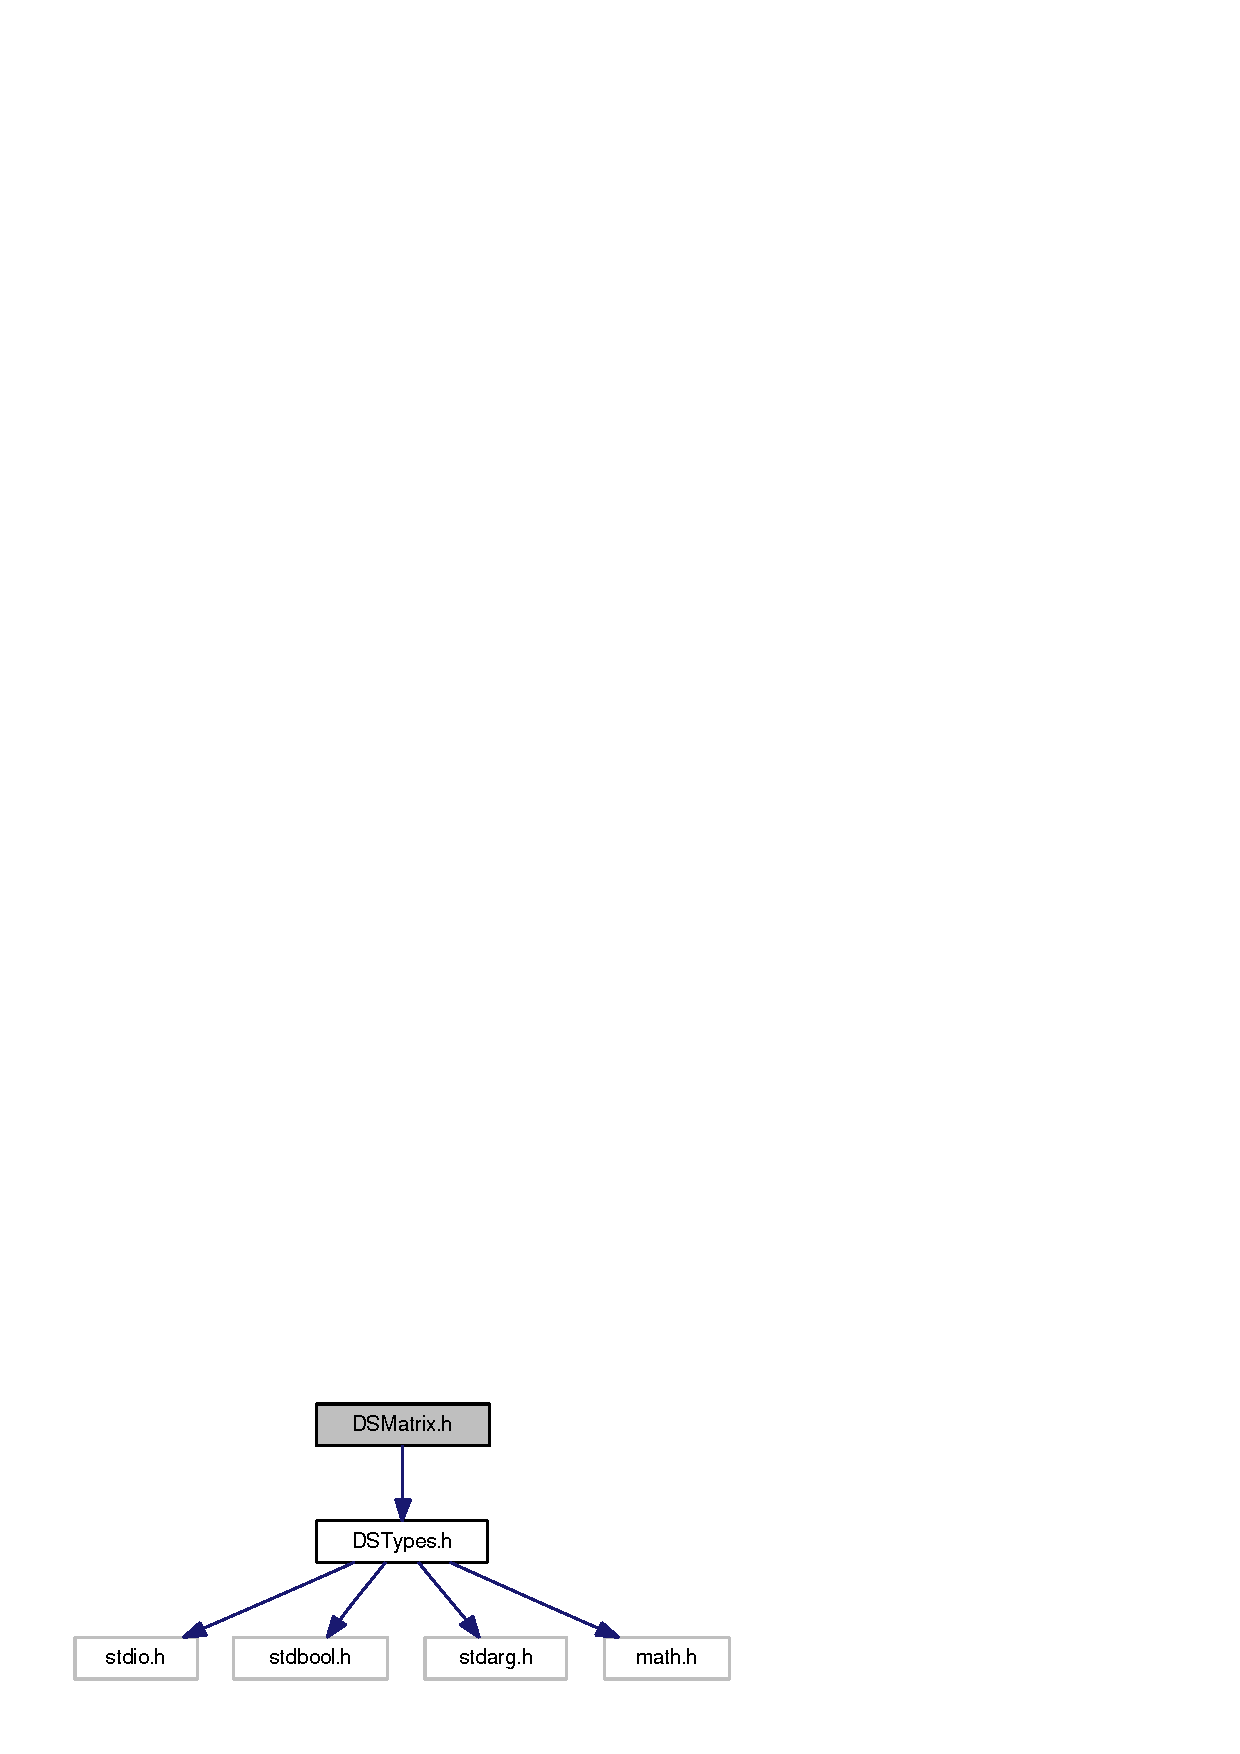
\includegraphics[width=175pt]{_d_s_matrix_8h__incl}
\end{center}
\end{figure}
This graph shows which files directly or indirectly include this file:\nopagebreak
\begin{figure}[H]
\begin{center}
\leavevmode
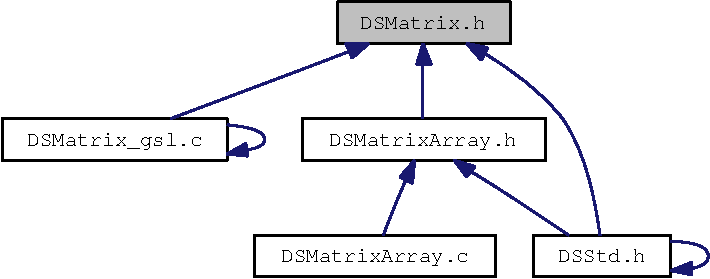
\includegraphics[width=188pt]{_d_s_matrix_8h__dep__incl}
\end{center}
\end{figure}
\subsection*{Defines}
\begin{DoxyCompactItemize}
\item 
\hypertarget{group___m___d_s___messages_gad80933e02bded8d239593be18ed3dea9}{
\#define \hyperlink{group___m___d_s___messages_gad80933e02bded8d239593be18ed3dea9}{M\_\-DS\_\-MAT\_\-NULL}~\char`\"{}Pointer to matrix is NULL\char`\"{}}
\label{group___m___d_s___messages_gad80933e02bded8d239593be18ed3dea9}

\begin{DoxyCompactList}\small\item\em Message for a NULL \hyperlink{struct_d_s_matrix}{DSMatrix} pointer. \item\end{DoxyCompactList}\item 
\hypertarget{group___m___d_s___messages_gaeb861d5820b984719e6f2ff0ed0d66d5}{
\#define \hyperlink{group___m___d_s___messages_gaeb861d5820b984719e6f2ff0ed0d66d5}{M\_\-DS\_\-MAT\_\-OUTOFBOUNDS}~\char`\"{}Row or column out of bounds\char`\"{}}
\label{group___m___d_s___messages_gaeb861d5820b984719e6f2ff0ed0d66d5}

\begin{DoxyCompactList}\small\item\em Message for a row or column exceeding matrix bounds. \item\end{DoxyCompactList}\item 
\hypertarget{group___m___d_s___messages_ga834bdead8f9b0e20331b57e051c7f379}{
\#define \hyperlink{group___m___d_s___messages_ga834bdead8f9b0e20331b57e051c7f379}{M\_\-DS\_\-MAT\_\-NOINTERNAL}~\char`\"{}Matrix data is empty\char`\"{}}
\label{group___m___d_s___messages_ga834bdead8f9b0e20331b57e051c7f379}

\begin{DoxyCompactList}\small\item\em Message for a NULL internal matrix structure. \item\end{DoxyCompactList}\item 
\hypertarget{_d_s_matrix_8h_a2b09d3d5984eb41f44dbe6e04de4e199}{
\#define {\bfseries DSMatrixRows}(x)~((x)-\/$>$rows)}
\label{_d_s_matrix_8h_a2b09d3d5984eb41f44dbe6e04de4e199}

\item 
\hypertarget{_d_s_matrix_8h_ad567f0726012769bbc813a1bebec8888}{
\#define {\bfseries DSMatrixColumns}(x)~((x)-\/$>$columns)}
\label{_d_s_matrix_8h_ad567f0726012769bbc813a1bebec8888}

\item 
\hypertarget{_d_s_matrix_8h_acba950eb01bc9fa81fa85aae457c8e5e}{
\#define {\bfseries DSMatrixInternalPointer}(x)~((x)-\/$>$mat)}
\label{_d_s_matrix_8h_acba950eb01bc9fa81fa85aae457c8e5e}

\end{DoxyCompactItemize}
\subsection*{Enumerations}
\begin{DoxyCompactItemize}
\item 
enum \{ {\bfseries \_\-\_\-MAT\_\-GSL\_\-\_\-}, 
{\bfseries \_\-\_\-MAT\_\-CLAPACK\_\-\_\-}
 \}
\end{DoxyCompactItemize}
\subsection*{Functions}
\begin{DoxyCompactItemize}
\item 
\hyperlink{struct_d_s_matrix}{DSMatrix} $\ast$ \hyperlink{_d_s_matrix_8h_abfe7884de06da66ce4bc46c7048d4e49}{DSMatrixAlloc} (const DSUInteger rows, const DSUInteger columns)
\begin{DoxyCompactList}\small\item\em Memory allocation for a \hyperlink{struct_d_s_matrix}{DSMatrix} using malloc. \item\end{DoxyCompactList}\item 
\hyperlink{struct_d_s_matrix}{DSMatrix} $\ast$ \hyperlink{_d_s_matrix_8h_a1b228ecc7be521c40160173fc1cecea2}{DSMatrixCalloc} (const DSUInteger rows, const DSUInteger columns)
\begin{DoxyCompactList}\small\item\em Memory allocation for a \hyperlink{struct_d_s_matrix}{DSMatrix} using calloc. \item\end{DoxyCompactList}\item 
\hyperlink{struct_d_s_matrix}{DSMatrix} $\ast$ \hyperlink{_d_s_matrix_8h_a6d0f0f74bdd85829ba07dd33f51cfa11}{DSMatrixCopy} (const \hyperlink{struct_d_s_matrix}{DSMatrix} $\ast$original)
\begin{DoxyCompactList}\small\item\em Copies a \hyperlink{struct_d_s_matrix}{DSMatrix}. \item\end{DoxyCompactList}\item 
void \hyperlink{_d_s_matrix_8h_ae5fc6bceef5e7e9e2c6300a86bdfb5fc}{DSMatrixFree} (\hyperlink{struct_d_s_matrix}{DSMatrix} $\ast$matrix)
\begin{DoxyCompactList}\small\item\em Freeing memory for \hyperlink{struct_d_s_matrix}{DSMatrix}. \item\end{DoxyCompactList}\item 
\hyperlink{struct_d_s_matrix}{DSMatrix} $\ast$ \hyperlink{_d_s_matrix_8h_a1636a4663250c4e54df28b35b121d27f}{DSMatrixIdentity} (const DSUInteger size)
\begin{DoxyCompactList}\small\item\em Allocates a new \hyperlink{struct_d_s_matrix}{DSMatrix} as an identity matrix. \item\end{DoxyCompactList}\item 
\hyperlink{struct_d_s_matrix}{DSMatrix} $\ast$ \hyperlink{_d_s_matrix_8h_a8980e6c6dc06dbbda9cde939cff831cc}{DSMatrixRandomNumbers} (const DSUInteger rows, const DSUInteger columns)
\begin{DoxyCompactList}\small\item\em Allocates a new \hyperlink{struct_d_s_matrix}{DSMatrix} with random values between 0 and 1. \item\end{DoxyCompactList}\item 
\hypertarget{_d_s_matrix_8h_ad542fab68c7147002d3e5d4b136f188b}{
\hyperlink{struct_d_s_matrix}{DSMatrix} $\ast$ {\bfseries DSMatrixWithVariablePoolValues} (const \hyperlink{struct__var_dictionary}{DSVariablePool} $\ast$variablePool)}
\label{_d_s_matrix_8h_ad542fab68c7147002d3e5d4b136f188b}

\item 
\hypertarget{_d_s_matrix_8h_acdf23ab773e0822d370c5cedf8ef52a6}{
void {\bfseries DSMatrixSetRows} (\hyperlink{struct_d_s_matrix}{DSMatrix} $\ast$matrix, const DSUInteger rows)}
\label{_d_s_matrix_8h_acdf23ab773e0822d370c5cedf8ef52a6}

\item 
\hypertarget{_d_s_matrix_8h_adf7db42a38601dc8ccc254aae94ab42d}{
void {\bfseries DSMatrixSetColumns} (\hyperlink{struct_d_s_matrix}{DSMatrix} $\ast$matrix, const DSUInteger columns)}
\label{_d_s_matrix_8h_adf7db42a38601dc8ccc254aae94ab42d}

\item 
double \hyperlink{_d_s_matrix_8h_abc810db5fab16f43f5279815726577de}{DSMatrixDoubleValue} (const \hyperlink{struct_d_s_matrix}{DSMatrix} $\ast$matrix, const DSUInteger row, const DSUInteger column)
\begin{DoxyCompactList}\small\item\em Returns the element of the \hyperlink{struct_d_s_matrix}{DSMatrix} specified by a row and column. \item\end{DoxyCompactList}\item 
\hypertarget{_d_s_matrix_8h_a78ca87769f9a2f7adaddaf89ddc4fe76}{
void {\bfseries DSMatrixSetDoubleValue} (\hyperlink{struct_d_s_matrix}{DSMatrix} $\ast$matrix, const DSUInteger row, const DSUInteger column, const double value)}
\label{_d_s_matrix_8h_a78ca87769f9a2f7adaddaf89ddc4fe76}

\item 
void \hyperlink{_d_s_matrix_8h_a9c9214fc02b42105ba79ed810aa5249f}{DSMatrixSetDoubleValueAll} (\hyperlink{struct_d_s_matrix}{DSMatrix} $\ast$matrix, const double value)
\begin{DoxyCompactList}\small\item\em Sets all the values of a matrix to a value. \item\end{DoxyCompactList}\item 
\hypertarget{_d_s_matrix_8h_a8129ecd2a1b6b540bf990a1e0122df54}{
void {\bfseries DSMatrixSetDoubleValuesList} (\hyperlink{struct_d_s_matrix}{DSMatrix} $\ast$matrix, bool byColumns, DSUInteger numberOfValues, double firstValue,...)}
\label{_d_s_matrix_8h_a8129ecd2a1b6b540bf990a1e0122df54}

\item 
\hypertarget{_d_s_matrix_8h_a19ad8529f691fe79db86bd0b2ef20f65}{
void {\bfseries DSMatrixSetDoubleValues} (\hyperlink{struct_d_s_matrix}{DSMatrix} $\ast$matrix, bool byColumns, DSUInteger numberOfValues, double $\ast$values)}
\label{_d_s_matrix_8h_a19ad8529f691fe79db86bd0b2ef20f65}

\item 
\hypertarget{_d_s_matrix_8h_abbfa6df7989a2d75edd5352dc1a88958}{
void {\bfseries DSMatrixRoundToSignificantFigures} (\hyperlink{struct_d_s_matrix}{DSMatrix} $\ast$matrix, const unsigned char figures)}
\label{_d_s_matrix_8h_abbfa6df7989a2d75edd5352dc1a88958}

\item 
\hypertarget{_d_s_matrix_8h_a13722367c1d0a25a9c4e2494a69d036e}{
\hyperlink{struct_d_s_matrix}{DSMatrix} $\ast$ {\bfseries DSMatrixSubMatrixExcludingColumnList} (const \hyperlink{struct_d_s_matrix}{DSMatrix} $\ast$matrix, const DSUInteger numberOfColumns, const DSUInteger firstColumn,...)}
\label{_d_s_matrix_8h_a13722367c1d0a25a9c4e2494a69d036e}

\item 
\hypertarget{_d_s_matrix_8h_aa316043dd2ecd826dc7606c8b41c480a}{
\hyperlink{struct_d_s_matrix}{DSMatrix} $\ast$ {\bfseries DSMatrixSubMatrixExcludingColumns} (const \hyperlink{struct_d_s_matrix}{DSMatrix} $\ast$matrix, const DSUInteger numberOfColumns, const DSUInteger $\ast$columns)}
\label{_d_s_matrix_8h_aa316043dd2ecd826dc7606c8b41c480a}

\item 
\hypertarget{_d_s_matrix_8h_a8e7e85c7bcef174c73eb6ab184e7edff}{
\hyperlink{struct_d_s_matrix}{DSMatrix} $\ast$ {\bfseries DSMatrixSubMatrixExcludingRowList} (const \hyperlink{struct_d_s_matrix}{DSMatrix} $\ast$matrix, const DSUInteger numberOfRows, const DSUInteger firstRow,...)}
\label{_d_s_matrix_8h_a8e7e85c7bcef174c73eb6ab184e7edff}

\item 
\hypertarget{_d_s_matrix_8h_ab8362aa8c8a7914570fbd399086c0163}{
\hyperlink{struct_d_s_matrix}{DSMatrix} $\ast$ {\bfseries DSMatrixSubMatrixExcludingRows} (const \hyperlink{struct_d_s_matrix}{DSMatrix} $\ast$matrix, const DSUInteger numberOfRows, const DSUInteger $\ast$rows)}
\label{_d_s_matrix_8h_ab8362aa8c8a7914570fbd399086c0163}

\item 
\hypertarget{_d_s_matrix_8h_a2b65f2d88e005e3bc9557cff4ff126d4}{
\hyperlink{struct_d_s_matrix}{DSMatrix} $\ast$ {\bfseries DSMatrixSubMatrixIncludingRowList} (const \hyperlink{struct_d_s_matrix}{DSMatrix} $\ast$matrix, const DSUInteger numberOfRows, const DSUInteger firstRow,...)}
\label{_d_s_matrix_8h_a2b65f2d88e005e3bc9557cff4ff126d4}

\item 
\hypertarget{_d_s_matrix_8h_a676818b51f086fe381dcdad273a6b4bd}{
\hyperlink{struct_d_s_matrix}{DSMatrix} $\ast$ {\bfseries DSMatrixSubMatrixIncludingRows} (const \hyperlink{struct_d_s_matrix}{DSMatrix} $\ast$matrix, const DSUInteger numberOfRows, const DSUInteger $\ast$rows)}
\label{_d_s_matrix_8h_a676818b51f086fe381dcdad273a6b4bd}

\item 
\hypertarget{_d_s_matrix_8h_a3f4ccfa4e6f945f8020a8c8140078b89}{
\hyperlink{struct_d_s_matrix}{DSMatrix} $\ast$ {\bfseries DSMatrixSubMatrixIncludingColumnList} (const \hyperlink{struct_d_s_matrix}{DSMatrix} $\ast$matrix, const DSUInteger numberOfColumns, const DSUInteger firstColumn,...)}
\label{_d_s_matrix_8h_a3f4ccfa4e6f945f8020a8c8140078b89}

\item 
\hypertarget{_d_s_matrix_8h_ae4bb2ee0b4eb036d971cf88fb7e1e073}{
\hyperlink{struct_d_s_matrix}{DSMatrix} $\ast$ {\bfseries DSMatrixSubMatrixExcludingRowAndColumnList} (const \hyperlink{struct_d_s_matrix}{DSMatrix} $\ast$matrix, const DSUInteger numberOfRows, const DSUInteger numberOfColumns, const DSUInteger firstRow,...)}
\label{_d_s_matrix_8h_ae4bb2ee0b4eb036d971cf88fb7e1e073}

\item 
\hypertarget{_d_s_matrix_8h_a9cd9bc2e0f687b8e8716d2da805a0cd9}{
\hyperlink{struct_d_s_matrix}{DSMatrix} $\ast$ {\bfseries DSMatrixSubMatrixExcludingRowsAndColumns} (const \hyperlink{struct_d_s_matrix}{DSMatrix} $\ast$matrix, const DSUInteger numberOfRows, const DSUInteger numberOfColumns, const DSUInteger $\ast$rows, const DSUInteger $\ast$columns)}
\label{_d_s_matrix_8h_a9cd9bc2e0f687b8e8716d2da805a0cd9}

\item 
\hypertarget{_d_s_matrix_8h_ae76009a59653b8199de1aef298aab22a}{
\hyperlink{struct_d_s_matrix}{DSMatrix} $\ast$ {\bfseries DSMatrixSubMatrixIncludingColumns} (const \hyperlink{struct_d_s_matrix}{DSMatrix} $\ast$matrix, const DSUInteger numberOfColumns, const DSUInteger $\ast$columns)}
\label{_d_s_matrix_8h_ae76009a59653b8199de1aef298aab22a}

\item 
\hypertarget{_d_s_matrix_8h_a46ee83c0131a233a3fc383fa25eb39a8}{
\hyperlink{struct_d_s_matrix}{DSMatrix} $\ast$ {\bfseries DSMatrixSubMatrixIncludingRowAndColumnList} (const \hyperlink{struct_d_s_matrix}{DSMatrix} $\ast$matrix, const DSUInteger numberOfRows, const DSUInteger numberOfColumns, const DSUInteger firstRow,...)}
\label{_d_s_matrix_8h_a46ee83c0131a233a3fc383fa25eb39a8}

\item 
\hypertarget{_d_s_matrix_8h_a57c83410ea80f8273aed426b1ee97edb}{
\hyperlink{struct_d_s_matrix}{DSMatrix} $\ast$ {\bfseries DSMatrixAppendMatrices} (const \hyperlink{struct_d_s_matrix}{DSMatrix} $\ast$firstMatrix, const \hyperlink{struct_d_s_matrix}{DSMatrix} $\ast$secondMatrix, const bool byColumn)}
\label{_d_s_matrix_8h_a57c83410ea80f8273aed426b1ee97edb}

\item 
\hypertarget{_d_s_matrix_8h_a915840fcecbdf1d22f012c4dfe1b9865}{
void {\bfseries DSMatrixSwitchRows} (\hyperlink{struct_d_s_matrix}{DSMatrix} $\ast$matrix, const DSUInteger rowA, const DSUInteger rowB)}
\label{_d_s_matrix_8h_a915840fcecbdf1d22f012c4dfe1b9865}

\item 
\hypertarget{_d_s_matrix_8h_aef190e8f762eb55b71830a4b9b6ce029}{
void {\bfseries DSMatrixSwitchColumns} (\hyperlink{struct_d_s_matrix}{DSMatrix} $\ast$matrix, const DSUInteger columnA, const DSUInteger columnB)}
\label{_d_s_matrix_8h_aef190e8f762eb55b71830a4b9b6ce029}

\item 
\hypertarget{_d_s_matrix_8h_aafc2224cfb968cc0ec445fb547a1a1f8}{
void {\bfseries DSMatrixPrint} (\hyperlink{struct_d_s_matrix}{DSMatrix} $\ast$matrix)}
\label{_d_s_matrix_8h_aafc2224cfb968cc0ec445fb547a1a1f8}

\item 
\hypertarget{_d_s_matrix_8h_aab4e40a4f3db7f41a1f24a106b0bcaae}{
bool {\bfseries DSMatrixIsIdentity} (const \hyperlink{struct_d_s_matrix}{DSMatrix} $\ast$matrix)}
\label{_d_s_matrix_8h_aab4e40a4f3db7f41a1f24a106b0bcaae}

\item 
\hypertarget{_d_s_matrix_8h_ad26bbf7bce64f29ce88055fee6573d86}{
bool {\bfseries DSMatrixIsSquare} (const \hyperlink{struct_d_s_matrix}{DSMatrix} $\ast$matrix)}
\label{_d_s_matrix_8h_ad26bbf7bce64f29ce88055fee6573d86}

\item 
\hypertarget{_d_s_matrix_8h_ac32edf137c13f9d5807c149dacee3a6e}{
DSUInteger {\bfseries DSMatrixRank} (const \hyperlink{struct_d_s_matrix}{DSMatrix} $\ast$matrix)}
\label{_d_s_matrix_8h_ac32edf137c13f9d5807c149dacee3a6e}

\item 
\hypertarget{_d_s_matrix_8h_aaf9d20837b2f87c74a454100429b64ac}{
double {\bfseries minimumValue} (const \hyperlink{struct_d_s_matrix}{DSMatrix} $\ast$matrix, const bool shouldExcludeZero)}
\label{_d_s_matrix_8h_aaf9d20837b2f87c74a454100429b64ac}

\item 
\hypertarget{_d_s_matrix_8h_acf33f61fc91fd02dacfbc31c6ffeeaf8}{
double {\bfseries maximumValue} (const \hyperlink{struct_d_s_matrix}{DSMatrix} $\ast$matrix, const bool shouldExcludeZero)}
\label{_d_s_matrix_8h_acf33f61fc91fd02dacfbc31c6ffeeaf8}

\item 
\hypertarget{_d_s_matrix_8h_a3205b0946508ed84873347cafacd5eb3}{
\hyperlink{struct_d_s_matrix}{DSMatrix} $\ast$ {\bfseries DSMatrixBySubstractingMatrix} (const \hyperlink{struct_d_s_matrix}{DSMatrix} $\ast$lvalue, const \hyperlink{struct_d_s_matrix}{DSMatrix} $\ast$rvalue)}
\label{_d_s_matrix_8h_a3205b0946508ed84873347cafacd5eb3}

\item 
\hypertarget{_d_s_matrix_8h_aa1c9f578946f7d5fe69d5e4a1ebaaadf}{
\hyperlink{struct_d_s_matrix}{DSMatrix} $\ast$ {\bfseries DSMatrixByAddingMatrix} (const \hyperlink{struct_d_s_matrix}{DSMatrix} $\ast$lvalue, const \hyperlink{struct_d_s_matrix}{DSMatrix} $\ast$rvalue)}
\label{_d_s_matrix_8h_aa1c9f578946f7d5fe69d5e4a1ebaaadf}

\item 
\hypertarget{_d_s_matrix_8h_aecdf05e600ce503d4e54ae43720bde8d}{
\hyperlink{struct_d_s_matrix}{DSMatrix} $\ast$ {\bfseries DSMatrixByDividingMatrix} (const \hyperlink{struct_d_s_matrix}{DSMatrix} $\ast$lvalue, const \hyperlink{struct_d_s_matrix}{DSMatrix} $\ast$rvalue)}
\label{_d_s_matrix_8h_aecdf05e600ce503d4e54ae43720bde8d}

\item 
\hyperlink{struct_d_s_matrix}{DSMatrix} $\ast$ \hyperlink{_d_s_matrix_8h_a6ca3f3a56a30db46fdfa2035121515da}{DSMatrixByMultiplyingMatrix} (const \hyperlink{struct_d_s_matrix}{DSMatrix} $\ast$lvalue, const \hyperlink{struct_d_s_matrix}{DSMatrix} $\ast$rvalue)
\item 
\hypertarget{_d_s_matrix_8h_a9dbd160849a73f61a42f9356daac2d8f}{
\hyperlink{struct_d_s_matrix}{DSMatrix} $\ast$ {\bfseries DSMatrixByApplyingFunction} (const \hyperlink{struct_d_s_matrix}{DSMatrix} $\ast$mvalue, double($\ast$function)(double))}
\label{_d_s_matrix_8h_a9dbd160849a73f61a42f9356daac2d8f}

\item 
\hypertarget{_d_s_matrix_8h_a70c586f979ed9697ba532079a063e482}{
\hyperlink{struct_d_s_matrix}{DSMatrix} $\ast$ {\bfseries DSMatrixBySubstractingScalar} (const \hyperlink{struct_d_s_matrix}{DSMatrix} $\ast$lvalue, const double rvalue)}
\label{_d_s_matrix_8h_a70c586f979ed9697ba532079a063e482}

\item 
\hypertarget{_d_s_matrix_8h_af75d930f6cd98e4df848415456614aea}{
\hyperlink{struct_d_s_matrix}{DSMatrix} $\ast$ {\bfseries DSMatrixByAddingScalar} (const \hyperlink{struct_d_s_matrix}{DSMatrix} $\ast$lvalue, const double rvalue)}
\label{_d_s_matrix_8h_af75d930f6cd98e4df848415456614aea}

\item 
\hypertarget{_d_s_matrix_8h_a60b24f071ca4800d11c597e01972cd92}{
\hyperlink{struct_d_s_matrix}{DSMatrix} $\ast$ {\bfseries DSMatrixByDividingScalar} (const \hyperlink{struct_d_s_matrix}{DSMatrix} $\ast$lvalue, const double rvalue)}
\label{_d_s_matrix_8h_a60b24f071ca4800d11c597e01972cd92}

\item 
\hypertarget{_d_s_matrix_8h_a85636b6b07304278117d244ea9ae2dfe}{
\hyperlink{struct_d_s_matrix}{DSMatrix} $\ast$ {\bfseries DSMatrixByMultiplyingScalar} (const \hyperlink{struct_d_s_matrix}{DSMatrix} $\ast$lvalue, const double rvalue)}
\label{_d_s_matrix_8h_a85636b6b07304278117d244ea9ae2dfe}

\item 
\hypertarget{_d_s_matrix_8h_a81c24f3537a442778c36dc1168104a18}{
double {\bfseries DSMatrixDeterminant} (const \hyperlink{struct_d_s_matrix}{DSMatrix} $\ast$matrix)}
\label{_d_s_matrix_8h_a81c24f3537a442778c36dc1168104a18}

\item 
\hypertarget{_d_s_matrix_8h_a5d09ce999ee6fcf460e16cfb65e9718c}{
\hyperlink{struct_d_s_matrix}{DSMatrix} $\ast$ {\bfseries DSMatrixTranspose} (const \hyperlink{struct_d_s_matrix}{DSMatrix} $\ast$matrix)}
\label{_d_s_matrix_8h_a5d09ce999ee6fcf460e16cfb65e9718c}

\item 
\hypertarget{_d_s_matrix_8h_a915bc15d3860a97f471e06da2787ed40}{
\hyperlink{struct_d_s_matrix}{DSMatrix} $\ast$ {\bfseries DSMatrixInverse} (const \hyperlink{struct_d_s_matrix}{DSMatrix} $\ast$matrix)}
\label{_d_s_matrix_8h_a915bc15d3860a97f471e06da2787ed40}

\item 
\hypertarget{_d_s_matrix_8h_af390e9c84b553fd7b5454d8bcc846f3b}{
\hyperlink{struct_d_s_matrix_array}{DSMatrixArray} $\ast$ {\bfseries DSMatrixSVD} (const \hyperlink{struct_d_s_matrix}{DSMatrix} $\ast$matrix)}
\label{_d_s_matrix_8h_af390e9c84b553fd7b5454d8bcc846f3b}

\item 
\hypertarget{_d_s_matrix_8h_a363c4377a0f3545bc686bc63845f36b3}{
\hyperlink{struct_d_s_matrix}{DSMatrix} $\ast$ {\bfseries DSMatrixRightNullspace} (const \hyperlink{struct_d_s_matrix}{DSMatrix} $\ast$matrix)}
\label{_d_s_matrix_8h_a363c4377a0f3545bc686bc63845f36b3}

\item 
\hyperlink{struct_d_s_matrix_array}{DSMatrixArray} $\ast$ \hyperlink{_d_s_matrix_8h_a419eb1fe1c418be7c59b10ce49a78b02}{DSMatrixPLUDecomposition} (const \hyperlink{struct_d_s_matrix}{DSMatrix} $\ast$matrix)
\begin{DoxyCompactList}\small\item\em Creates a LU decomposition and returns the permutation matrix. \item\end{DoxyCompactList}\item 
\hypertarget{_d_s_matrix_8h_a30f30a57d317b99eee2d0e5d55cb3a5c}{
double $\ast$ {\bfseries DSMatrixDataForGLPK} (const \hyperlink{struct_d_s_matrix}{DSMatrix} $\ast$matrix)}
\label{_d_s_matrix_8h_a30f30a57d317b99eee2d0e5d55cb3a5c}

\item 
\hypertarget{_d_s_matrix_8h_a799843ba9eaf47d02779a42f07cefd30}{
int $\ast$ {\bfseries DSMatrixRowsForGLPK} (const \hyperlink{struct_d_s_matrix}{DSMatrix} $\ast$matrix)}
\label{_d_s_matrix_8h_a799843ba9eaf47d02779a42f07cefd30}

\item 
\hypertarget{_d_s_matrix_8h_afd2ac8850f5d1b51684e5ded7ee81f63}{
int $\ast$ {\bfseries DSMatrixColumnsForGLPK} (const \hyperlink{struct_d_s_matrix}{DSMatrix} $\ast$matrix)}
\label{_d_s_matrix_8h_afd2ac8850f5d1b51684e5ded7ee81f63}

\end{DoxyCompactItemize}


\subsection{Detailed Description}
Header file with functions for dealing with matrices. Copyright (C) 2011 Jason Lomnitz.\par
\par


This file is part of the Design Space Toolbox V2 (C Library).

The Design Space Toolbox V2 is free software: you can redistribute it and/or modify it under the terms of the GNU General Public License as published by the Free Software Foundation, either version 3 of the License, or (at your option) any later version.

The Design Space Toolbox V2 is distributed in the hope that it will be useful, but WITHOUT ANY WARRANTY; without even the implied warranty of MERCHANTABILITY or FITNESS FOR A PARTICULAR PURPOSE. See the GNU General Public License for more details.

You should have received a copy of the GNU General Public License along with the Design Space Toolbox. If not, see $<$\href{http://www.gnu.org/licenses/}{\tt http://www.gnu.org/licenses/}$>$.

\begin{DoxyAuthor}{Author}
Jason Lomnitz. 
\end{DoxyAuthor}
\begin{DoxyDate}{Date}
2011 
\end{DoxyDate}


\subsection{Function Documentation}
\hypertarget{_d_s_matrix_8h_abfe7884de06da66ce4bc46c7048d4e49}{
\index{DSMatrix.h@{DSMatrix.h}!DSMatrixAlloc@{DSMatrixAlloc}}
\index{DSMatrixAlloc@{DSMatrixAlloc}!DSMatrix.h@{DSMatrix.h}}
\subsubsection[{DSMatrixAlloc}]{\setlength{\rightskip}{0pt plus 5cm}{\bf DSMatrix}$\ast$ DSMatrixAlloc (const DSUInteger {\em rows}, \/  const DSUInteger {\em columns})}}
\label{_d_s_matrix_8h_abfe7884de06da66ce4bc46c7048d4e49}


Memory allocation for a \hyperlink{struct_d_s_matrix}{DSMatrix} using malloc. 

Creates a new matrix of a particular size. The matrix that is allocated has all the values of the matrix defaulted to 0. The internal matrix pointer must be set to NULL; otherwise, the size of the matrix cannot be changed.


\begin{DoxyParams}{Parameters}
\item[{\em rows}]A DSUInteger with the number of rows in the new matrix. \item[{\em columns}]A DSUInteger with the number of columns in the new matrix.\end{DoxyParams}
\begin{DoxyReturn}{Returns}
If the matrix was created, a new pointer to a \hyperlink{struct_d_s_matrix}{DSMatrix} is returned. Otherwise, NULL is returned. 
\end{DoxyReturn}
\hypertarget{_d_s_matrix_8h_a6ca3f3a56a30db46fdfa2035121515da}{
\index{DSMatrix.h@{DSMatrix.h}!DSMatrixByMultiplyingMatrix@{DSMatrixByMultiplyingMatrix}}
\index{DSMatrixByMultiplyingMatrix@{DSMatrixByMultiplyingMatrix}!DSMatrix.h@{DSMatrix.h}}
\subsubsection[{DSMatrixByMultiplyingMatrix}]{\setlength{\rightskip}{0pt plus 5cm}{\bf DSMatrix}$\ast$ DSMatrixByMultiplyingMatrix (const {\bf DSMatrix} $\ast$ {\em lvalue}, \/  const {\bf DSMatrix} $\ast$ {\em rvalue})}}
\label{_d_s_matrix_8h_a6ca3f3a56a30db46fdfa2035121515da}
Multiplication by a matrix inverse or pseudoinverse \hypertarget{_d_s_matrix_8h_a1b228ecc7be521c40160173fc1cecea2}{
\index{DSMatrix.h@{DSMatrix.h}!DSMatrixCalloc@{DSMatrixCalloc}}
\index{DSMatrixCalloc@{DSMatrixCalloc}!DSMatrix.h@{DSMatrix.h}}
\subsubsection[{DSMatrixCalloc}]{\setlength{\rightskip}{0pt plus 5cm}{\bf DSMatrix}$\ast$ DSMatrixCalloc (const DSUInteger {\em rows}, \/  const DSUInteger {\em columns})}}
\label{_d_s_matrix_8h_a1b228ecc7be521c40160173fc1cecea2}


Memory allocation for a \hyperlink{struct_d_s_matrix}{DSMatrix} using calloc. 

Creates a new matrix of a particular size. The matrix that is allocated has all the values of the matrix defaulted to 0. The internal matrix pointer must be set to NULL; otherwise, the size of the matrix cannot be changed.


\begin{DoxyParams}{Parameters}
\item[{\em rows}]A DSUInteger with the number of rows in the new matrix. \item[{\em columns}]A DSUInteger with the number of columns in the new matrix.\end{DoxyParams}
\begin{DoxyReturn}{Returns}
If the matrix was created, a new pointer to a \hyperlink{struct_d_s_matrix}{DSMatrix} is returned. Otherwise, NULL is returned. 
\end{DoxyReturn}
\hypertarget{_d_s_matrix_8h_a6d0f0f74bdd85829ba07dd33f51cfa11}{
\index{DSMatrix.h@{DSMatrix.h}!DSMatrixCopy@{DSMatrixCopy}}
\index{DSMatrixCopy@{DSMatrixCopy}!DSMatrix.h@{DSMatrix.h}}
\subsubsection[{DSMatrixCopy}]{\setlength{\rightskip}{0pt plus 5cm}{\bf DSMatrix}$\ast$ DSMatrixCopy (const {\bf DSMatrix} $\ast$ {\em original})}}
\label{_d_s_matrix_8h_a6d0f0f74bdd85829ba07dd33f51cfa11}


Copies a \hyperlink{struct_d_s_matrix}{DSMatrix}. 

Creates a new matrix with the exact same size and contents as some other matrix. The new matrix is allocated, and thus must be freed.


\begin{DoxyParams}{Parameters}
\item[{\em original}]The \hyperlink{struct_d_s_matrix}{DSMatrix} to be copied.\end{DoxyParams}
\begin{DoxyReturn}{Returns}
If the copy was succesful, a pointer to a copy of the \hyperlink{struct_d_s_matrix}{DSMatrix} is returned. Otherwise, NULL is returned. 
\end{DoxyReturn}
\hypertarget{_d_s_matrix_8h_abc810db5fab16f43f5279815726577de}{
\index{DSMatrix.h@{DSMatrix.h}!DSMatrixDoubleValue@{DSMatrixDoubleValue}}
\index{DSMatrixDoubleValue@{DSMatrixDoubleValue}!DSMatrix.h@{DSMatrix.h}}
\subsubsection[{DSMatrixDoubleValue}]{\setlength{\rightskip}{0pt plus 5cm}double DSMatrixDoubleValue (const {\bf DSMatrix} $\ast$ {\em matrix}, \/  const DSUInteger {\em row}, \/  const DSUInteger {\em column})}}
\label{_d_s_matrix_8h_abc810db5fab16f43f5279815726577de}


Returns the element of the \hyperlink{struct_d_s_matrix}{DSMatrix} specified by a row and column. 

Returns an element of the matrix, with indices i and j starting at 0.


\begin{DoxyParams}{Parameters}
\item[{\em matrix}]The \hyperlink{struct_d_s_matrix}{DSMatrix} whose elements will be accessed. \item[{\em row}]A DSUInteger specifying the row coordinate of the element to be accessed. \item[{\em column}]A DSUInteger specifying the column coordinate of the element to be accessed.\end{DoxyParams}
\begin{DoxyReturn}{Returns}
If the value was succesfully retrieved, the double value contained at the row and column coordinate of the \hyperlink{struct_d_s_matrix}{DSMatrix} is returned. Otherwise, NaN is returned. 
\end{DoxyReturn}
\hypertarget{_d_s_matrix_8h_ae5fc6bceef5e7e9e2c6300a86bdfb5fc}{
\index{DSMatrix.h@{DSMatrix.h}!DSMatrixFree@{DSMatrixFree}}
\index{DSMatrixFree@{DSMatrixFree}!DSMatrix.h@{DSMatrix.h}}
\subsubsection[{DSMatrixFree}]{\setlength{\rightskip}{0pt plus 5cm}void DSMatrixFree ({\bf DSMatrix} $\ast$ {\em matrix})}}
\label{_d_s_matrix_8h_ae5fc6bceef5e7e9e2c6300a86bdfb5fc}


Freeing memory for \hyperlink{struct_d_s_matrix}{DSMatrix}. 

Frees the memory associated with a \hyperlink{struct_d_s_matrix}{DSMatrix} data type. This function is a wrapper for the necessary steps needed to free the internal structure of the \hyperlink{struct_d_s_matrix}{DSMatrix} data type.


\begin{DoxyParams}{Parameters}
\item[{\em matrix}]The \hyperlink{struct_d_s_matrix}{DSMatrix} to be freed. \end{DoxyParams}
\hypertarget{_d_s_matrix_8h_a1636a4663250c4e54df28b35b121d27f}{
\index{DSMatrix.h@{DSMatrix.h}!DSMatrixIdentity@{DSMatrixIdentity}}
\index{DSMatrixIdentity@{DSMatrixIdentity}!DSMatrix.h@{DSMatrix.h}}
\subsubsection[{DSMatrixIdentity}]{\setlength{\rightskip}{0pt plus 5cm}{\bf DSMatrix}$\ast$ DSMatrixIdentity (const DSUInteger {\em size})}}
\label{_d_s_matrix_8h_a1636a4663250c4e54df28b35b121d27f}


Allocates a new \hyperlink{struct_d_s_matrix}{DSMatrix} as an identity matrix. 

Allocates a square matrix of a specified size, and initializes the diagonal values to 1 and all the other values to 0, creating an identity matrix. The new matrix is therefore an identity matrix.


\begin{DoxyParams}{Parameters}
\item[{\em size}]A DSUInteger containing the number of rows and columns in the matrix.\end{DoxyParams}
\begin{DoxyReturn}{Returns}
If the identity matrix was succesfully created, a pointer to the \hyperlink{struct_d_s_matrix}{DSMatrix} is returned. Otherwise, NULL is returned. 
\end{DoxyReturn}
\hypertarget{_d_s_matrix_8h_a419eb1fe1c418be7c59b10ce49a78b02}{
\index{DSMatrix.h@{DSMatrix.h}!DSMatrixPLUDecomposition@{DSMatrixPLUDecomposition}}
\index{DSMatrixPLUDecomposition@{DSMatrixPLUDecomposition}!DSMatrix.h@{DSMatrix.h}}
\subsubsection[{DSMatrixPLUDecomposition}]{\setlength{\rightskip}{0pt plus 5cm}{\bf DSMatrixArray}$\ast$ DSMatrixPLUDecomposition (const {\bf DSMatrix} $\ast$ {\em A})}}
\label{_d_s_matrix_8h_a419eb1fe1c418be7c59b10ce49a78b02}


Creates a LU decomposition and returns the permutation matrix. 

This function creates a LU decomposition of a \hyperlink{struct_d_s_matrix}{DSMatrix} A. This function creates an array of three matrices: a \hyperlink{struct_d_s_matrix}{DSMatrix} P, a \hyperlink{struct_d_s_matrix}{DSMatrix} L and a \hyperlink{struct_d_s_matrix}{DSMatrix} U; where $ P A = L U $.


\begin{DoxyParams}{Parameters}
\item[{\em A}]A \hyperlink{struct_d_s_matrix}{DSMatrix} containing the matrix to be decomposed. \end{DoxyParams}
\hypertarget{_d_s_matrix_8h_a8980e6c6dc06dbbda9cde939cff831cc}{
\index{DSMatrix.h@{DSMatrix.h}!DSMatrixRandomNumbers@{DSMatrixRandomNumbers}}
\index{DSMatrixRandomNumbers@{DSMatrixRandomNumbers}!DSMatrix.h@{DSMatrix.h}}
\subsubsection[{DSMatrixRandomNumbers}]{\setlength{\rightskip}{0pt plus 5cm}{\bf DSMatrix}$\ast$ DSMatrixRandomNumbers (const DSUInteger {\em rows}, \/  const DSUInteger {\em columns})}}
\label{_d_s_matrix_8h_a8980e6c6dc06dbbda9cde939cff831cc}


Allocates a new \hyperlink{struct_d_s_matrix}{DSMatrix} with random values between 0 and 1. 

Allocates a new \hyperlink{struct_d_s_matrix}{DSMatrix} with a specified size. The values of each of the entries in the matrix are randomly selected between 0 and 1.


\begin{DoxyParams}{Parameters}
\item[{\em rows}]A DSUInteger with the number of rows in the new matrix. \item[{\em columns}]A DSUInteger with the number of columns in the new matrix.\end{DoxyParams}
\begin{DoxyReturn}{Returns}
If the matrix was created, a new pointer to a \hyperlink{struct_d_s_matrix}{DSMatrix} is returned. Otherwise, NULL is returned. 
\end{DoxyReturn}
\hypertarget{_d_s_matrix_8h_a9c9214fc02b42105ba79ed810aa5249f}{
\index{DSMatrix.h@{DSMatrix.h}!DSMatrixSetDoubleValueAll@{DSMatrixSetDoubleValueAll}}
\index{DSMatrixSetDoubleValueAll@{DSMatrixSetDoubleValueAll}!DSMatrix.h@{DSMatrix.h}}
\subsubsection[{DSMatrixSetDoubleValueAll}]{\setlength{\rightskip}{0pt plus 5cm}void DSMatrixSetDoubleValueAll ({\bf DSMatrix} $\ast$ {\em matrix}, \/  const double {\em value})}}
\label{_d_s_matrix_8h_a9c9214fc02b42105ba79ed810aa5249f}


Sets all the values of a matrix to a value. 

This function does not allocate the necessary memory; instead it goes through all the rows and columns of the matrix, assigning them the specified value.


\begin{DoxyParams}{Parameters}
\item[{\em matrix}]The \hyperlink{struct_d_s_matrix}{DSMatrix} that will be assigned the value. \item[{\em value}]The double variable whose value will be assigned. \end{DoxyParams}

\hypertarget{_d_s_matrix__gsl_8c}{
\section{DSMatrix\_\-gsl.c File Reference}
\label{_d_s_matrix__gsl_8c}\index{DSMatrix\_\-gsl.c@{DSMatrix\_\-gsl.c}}
}


Implementation file with functions for dealing with matrices using the GNU Scientific Library (gsl).  


{\ttfamily \#include $<$time.h$>$}\par
{\ttfamily \#include $<$stdarg.h$>$}\par
{\ttfamily \#include \char`\"{}DSMatrix.h\char`\"{}}\par
{\ttfamily \#include \char`\"{}DSTypes.h\char`\"{}}\par
{\ttfamily \#include \char`\"{}DSErrors.h\char`\"{}}\par
{\ttfamily \#include \char`\"{}DSMemoryManager.h\char`\"{}}\par
{\ttfamily \#include \char`\"{}DSMatrix.h\char`\"{}}\par
{\ttfamily \#include $<$gsl/gsl\_\-linalg.h$>$}\par
{\ttfamily \#include $<$gsl/gsl\_\-blas.h$>$}\par
Include dependency graph for DSMatrix\_\-gsl.c:\nopagebreak
\begin{figure}[H]
\begin{center}
\leavevmode
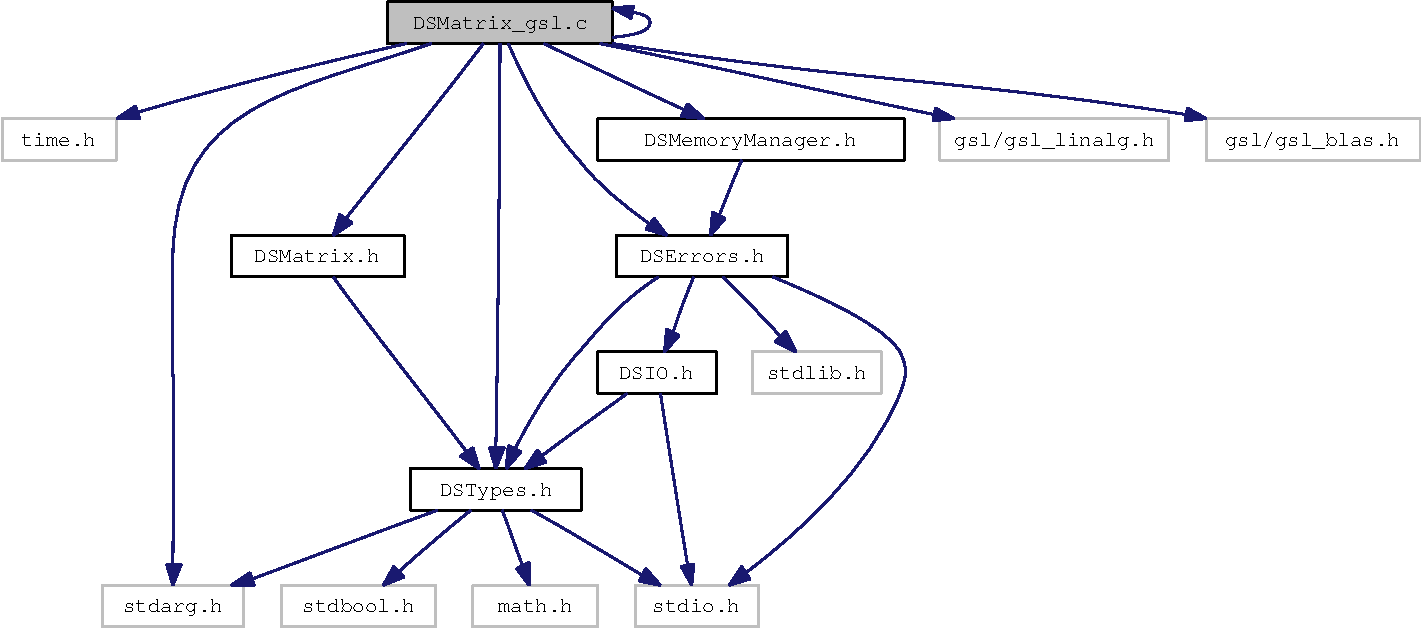
\includegraphics[width=358pt]{_d_s_matrix__gsl_8c__incl}
\end{center}
\end{figure}
This graph shows which files directly or indirectly include this file:\nopagebreak
\begin{figure}[H]
\begin{center}
\leavevmode
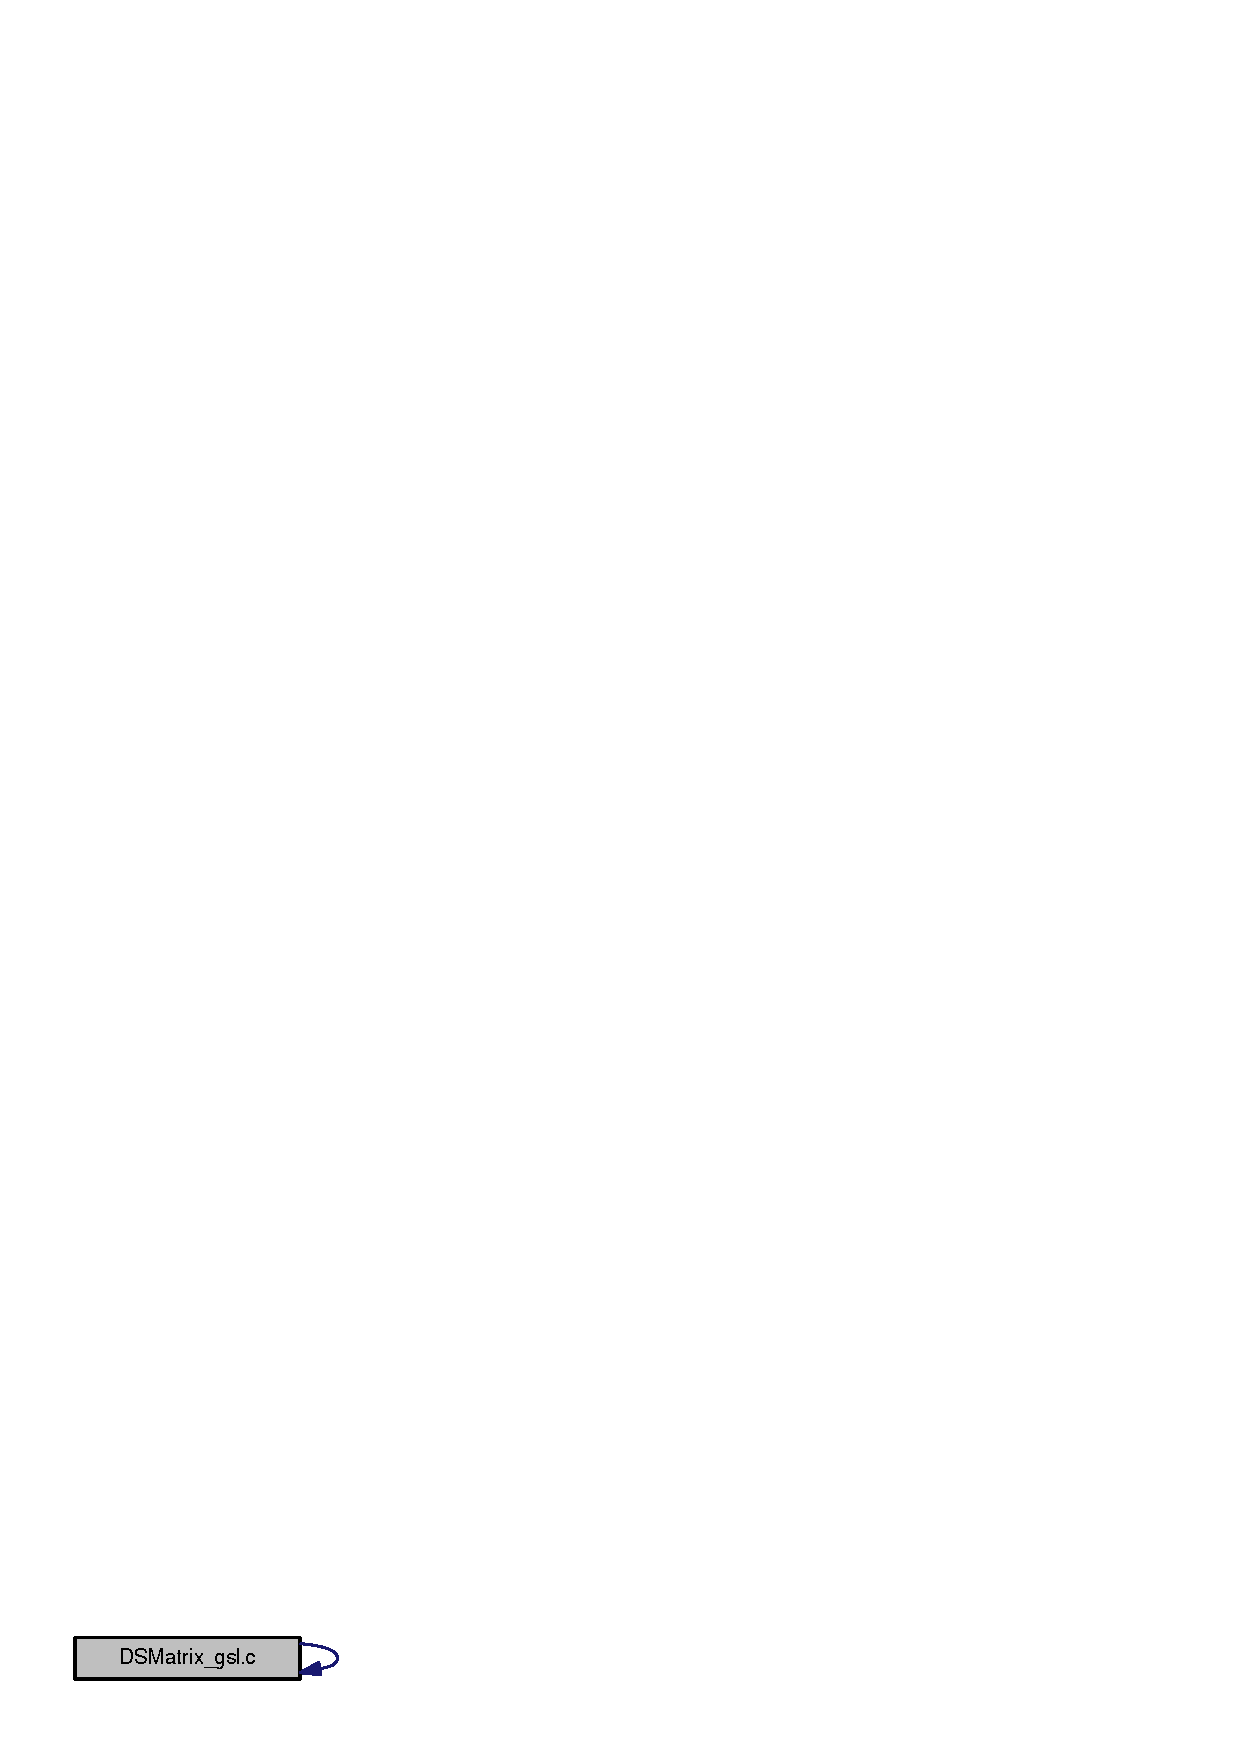
\includegraphics[width=81pt]{_d_s_matrix__gsl_8c__dep__incl}
\end{center}
\end{figure}
\subsection*{Functions}
\begin{DoxyCompactItemize}
\item 
\hyperlink{struct_d_s_matrix}{DSMatrix} $\ast$ \hyperlink{_d_s_matrix__gsl_8c_abfe7884de06da66ce4bc46c7048d4e49}{DSMatrixAlloc} (const DSUInteger rows, const DSUInteger columns)
\begin{DoxyCompactList}\small\item\em Memory allocation for a \hyperlink{struct_d_s_matrix}{DSMatrix} using malloc. \item\end{DoxyCompactList}\item 
\hyperlink{struct_d_s_matrix}{DSMatrix} $\ast$ \hyperlink{_d_s_matrix__gsl_8c_a1b228ecc7be521c40160173fc1cecea2}{DSMatrixCalloc} (const DSUInteger rows, const DSUInteger columns)
\begin{DoxyCompactList}\small\item\em Memory allocation for a \hyperlink{struct_d_s_matrix}{DSMatrix} using calloc. \item\end{DoxyCompactList}\item 
\hyperlink{struct_d_s_matrix}{DSMatrix} $\ast$ \hyperlink{_d_s_matrix__gsl_8c_a6d0f0f74bdd85829ba07dd33f51cfa11}{DSMatrixCopy} (const \hyperlink{struct_d_s_matrix}{DSMatrix} $\ast$original)
\begin{DoxyCompactList}\small\item\em Copies a \hyperlink{struct_d_s_matrix}{DSMatrix}. \item\end{DoxyCompactList}\item 
void \hyperlink{_d_s_matrix__gsl_8c_ae5fc6bceef5e7e9e2c6300a86bdfb5fc}{DSMatrixFree} (\hyperlink{struct_d_s_matrix}{DSMatrix} $\ast$matrix)
\begin{DoxyCompactList}\small\item\em Freeing memory for \hyperlink{struct_d_s_matrix}{DSMatrix}. \item\end{DoxyCompactList}\item 
\hyperlink{struct_d_s_matrix}{DSMatrix} $\ast$ \hyperlink{_d_s_matrix__gsl_8c_a1636a4663250c4e54df28b35b121d27f}{DSMatrixIdentity} (const DSUInteger size)
\begin{DoxyCompactList}\small\item\em Allocates a new \hyperlink{struct_d_s_matrix}{DSMatrix} as an identity matrix. \item\end{DoxyCompactList}\item 
\hyperlink{struct_d_s_matrix}{DSMatrix} $\ast$ \hyperlink{_d_s_matrix__gsl_8c_a8980e6c6dc06dbbda9cde939cff831cc}{DSMatrixRandomNumbers} (const DSUInteger rows, const DSUInteger columns)
\begin{DoxyCompactList}\small\item\em Allocates a new \hyperlink{struct_d_s_matrix}{DSMatrix} with random values between 0 and 1. \item\end{DoxyCompactList}\item 
\hypertarget{_d_s_matrix__gsl_8c_a3edb9316d7702cdb72c73e08b15a8158}{
\hyperlink{struct_d_s_matrix}{DSMatrix} $\ast$ {\bfseries DSMatrixWithVariablePoolValues} (const void $\ast$variablePool)}
\label{_d_s_matrix__gsl_8c_a3edb9316d7702cdb72c73e08b15a8158}

\item 
\hypertarget{_d_s_matrix__gsl_8c_abc810db5fab16f43f5279815726577de}{
double {\bfseries DSMatrixDoubleValue} (const \hyperlink{struct_d_s_matrix}{DSMatrix} $\ast$matrix, const DSUInteger row, const DSUInteger column)}
\label{_d_s_matrix__gsl_8c_abc810db5fab16f43f5279815726577de}

\item 
\hypertarget{_d_s_matrix__gsl_8c_acdf23ab773e0822d370c5cedf8ef52a6}{
void {\bfseries DSMatrixSetRows} (\hyperlink{struct_d_s_matrix}{DSMatrix} $\ast$matrix, const DSUInteger rows)}
\label{_d_s_matrix__gsl_8c_acdf23ab773e0822d370c5cedf8ef52a6}

\item 
\hypertarget{_d_s_matrix__gsl_8c_adf7db42a38601dc8ccc254aae94ab42d}{
void {\bfseries DSMatrixSetColumns} (\hyperlink{struct_d_s_matrix}{DSMatrix} $\ast$matrix, const DSUInteger columns)}
\label{_d_s_matrix__gsl_8c_adf7db42a38601dc8ccc254aae94ab42d}

\item 
\hypertarget{_d_s_matrix__gsl_8c_a78ca87769f9a2f7adaddaf89ddc4fe76}{
void {\bfseries DSMatrixSetDoubleValue} (\hyperlink{struct_d_s_matrix}{DSMatrix} $\ast$matrix, const DSUInteger row, const DSUInteger column, const double value)}
\label{_d_s_matrix__gsl_8c_a78ca87769f9a2f7adaddaf89ddc4fe76}

\item 
\hypertarget{_d_s_matrix__gsl_8c_a8129ecd2a1b6b540bf990a1e0122df54}{
void {\bfseries DSMatrixSetDoubleValuesList} (\hyperlink{struct_d_s_matrix}{DSMatrix} $\ast$matrix, bool byColumns, DSUInteger numberOfValues, double firstValue,...)}
\label{_d_s_matrix__gsl_8c_a8129ecd2a1b6b540bf990a1e0122df54}

\item 
\hypertarget{_d_s_matrix__gsl_8c_a19ad8529f691fe79db86bd0b2ef20f65}{
void {\bfseries DSMatrixSetDoubleValues} (\hyperlink{struct_d_s_matrix}{DSMatrix} $\ast$matrix, bool byColumns, DSUInteger numberOfValues, double $\ast$values)}
\label{_d_s_matrix__gsl_8c_a19ad8529f691fe79db86bd0b2ef20f65}

\item 
void \hyperlink{_d_s_matrix__gsl_8c_a9c9214fc02b42105ba79ed810aa5249f}{DSMatrixSetDoubleValueAll} (\hyperlink{struct_d_s_matrix}{DSMatrix} $\ast$matrix, const double value)
\begin{DoxyCompactList}\small\item\em Sets all the values of a matrix to a value. \item\end{DoxyCompactList}\item 
\hypertarget{_d_s_matrix__gsl_8c_abbfa6df7989a2d75edd5352dc1a88958}{
void {\bfseries DSMatrixRoundToSignificantFigures} (\hyperlink{struct_d_s_matrix}{DSMatrix} $\ast$matrix, const unsigned char figures)}
\label{_d_s_matrix__gsl_8c_abbfa6df7989a2d75edd5352dc1a88958}

\item 
\hypertarget{_d_s_matrix__gsl_8c_a8e7e85c7bcef174c73eb6ab184e7edff}{
\hyperlink{struct_d_s_matrix}{DSMatrix} $\ast$ {\bfseries DSMatrixSubMatrixExcludingRowList} (const \hyperlink{struct_d_s_matrix}{DSMatrix} $\ast$matrix, const DSUInteger numberOfRows, const DSUInteger firstRow,...)}
\label{_d_s_matrix__gsl_8c_a8e7e85c7bcef174c73eb6ab184e7edff}

\item 
\hypertarget{_d_s_matrix__gsl_8c_ab8362aa8c8a7914570fbd399086c0163}{
\hyperlink{struct_d_s_matrix}{DSMatrix} $\ast$ {\bfseries DSMatrixSubMatrixExcludingRows} (const \hyperlink{struct_d_s_matrix}{DSMatrix} $\ast$matrix, const DSUInteger numberOfRows, const DSUInteger $\ast$rows)}
\label{_d_s_matrix__gsl_8c_ab8362aa8c8a7914570fbd399086c0163}

\item 
\hypertarget{_d_s_matrix__gsl_8c_a13722367c1d0a25a9c4e2494a69d036e}{
\hyperlink{struct_d_s_matrix}{DSMatrix} $\ast$ {\bfseries DSMatrixSubMatrixExcludingColumnList} (const \hyperlink{struct_d_s_matrix}{DSMatrix} $\ast$matrix, const DSUInteger numberOfColumns, const DSUInteger firstColumn,...)}
\label{_d_s_matrix__gsl_8c_a13722367c1d0a25a9c4e2494a69d036e}

\item 
\hypertarget{_d_s_matrix__gsl_8c_aa316043dd2ecd826dc7606c8b41c480a}{
\hyperlink{struct_d_s_matrix}{DSMatrix} $\ast$ {\bfseries DSMatrixSubMatrixExcludingColumns} (const \hyperlink{struct_d_s_matrix}{DSMatrix} $\ast$matrix, const DSUInteger numberOfColumns, const DSUInteger $\ast$columns)}
\label{_d_s_matrix__gsl_8c_aa316043dd2ecd826dc7606c8b41c480a}

\item 
\hypertarget{_d_s_matrix__gsl_8c_a2b65f2d88e005e3bc9557cff4ff126d4}{
\hyperlink{struct_d_s_matrix}{DSMatrix} $\ast$ {\bfseries DSMatrixSubMatrixIncludingRowList} (const \hyperlink{struct_d_s_matrix}{DSMatrix} $\ast$matrix, const DSUInteger numberOfRows, const DSUInteger firstRow,...)}
\label{_d_s_matrix__gsl_8c_a2b65f2d88e005e3bc9557cff4ff126d4}

\item 
\hypertarget{_d_s_matrix__gsl_8c_a676818b51f086fe381dcdad273a6b4bd}{
\hyperlink{struct_d_s_matrix}{DSMatrix} $\ast$ {\bfseries DSMatrixSubMatrixIncludingRows} (const \hyperlink{struct_d_s_matrix}{DSMatrix} $\ast$matrix, const DSUInteger numberOfRows, const DSUInteger $\ast$rows)}
\label{_d_s_matrix__gsl_8c_a676818b51f086fe381dcdad273a6b4bd}

\item 
\hypertarget{_d_s_matrix__gsl_8c_a3f4ccfa4e6f945f8020a8c8140078b89}{
\hyperlink{struct_d_s_matrix}{DSMatrix} $\ast$ {\bfseries DSMatrixSubMatrixIncludingColumnList} (const \hyperlink{struct_d_s_matrix}{DSMatrix} $\ast$matrix, const DSUInteger numberOfColumns, const DSUInteger firstColumn,...)}
\label{_d_s_matrix__gsl_8c_a3f4ccfa4e6f945f8020a8c8140078b89}

\item 
\hypertarget{_d_s_matrix__gsl_8c_ae76009a59653b8199de1aef298aab22a}{
\hyperlink{struct_d_s_matrix}{DSMatrix} $\ast$ {\bfseries DSMatrixSubMatrixIncludingColumns} (const \hyperlink{struct_d_s_matrix}{DSMatrix} $\ast$matrix, const DSUInteger numberOfColumns, const DSUInteger $\ast$columns)}
\label{_d_s_matrix__gsl_8c_ae76009a59653b8199de1aef298aab22a}

\item 
\hypertarget{_d_s_matrix__gsl_8c_ae4bb2ee0b4eb036d971cf88fb7e1e073}{
\hyperlink{struct_d_s_matrix}{DSMatrix} $\ast$ {\bfseries DSMatrixSubMatrixExcludingRowAndColumnList} (const \hyperlink{struct_d_s_matrix}{DSMatrix} $\ast$matrix, const DSUInteger numberOfRows, const DSUInteger numberOfColumns, const DSUInteger firstRow,...)}
\label{_d_s_matrix__gsl_8c_ae4bb2ee0b4eb036d971cf88fb7e1e073}

\item 
\hypertarget{_d_s_matrix__gsl_8c_a9cd9bc2e0f687b8e8716d2da805a0cd9}{
\hyperlink{struct_d_s_matrix}{DSMatrix} $\ast$ {\bfseries DSMatrixSubMatrixExcludingRowsAndColumns} (const \hyperlink{struct_d_s_matrix}{DSMatrix} $\ast$matrix, const DSUInteger numberOfRows, const DSUInteger numberOfColumns, const DSUInteger $\ast$rows, const DSUInteger $\ast$columns)}
\label{_d_s_matrix__gsl_8c_a9cd9bc2e0f687b8e8716d2da805a0cd9}

\item 
\hypertarget{_d_s_matrix__gsl_8c_a46ee83c0131a233a3fc383fa25eb39a8}{
\hyperlink{struct_d_s_matrix}{DSMatrix} $\ast$ {\bfseries DSMatrixSubMatrixIncludingRowAndColumnList} (const \hyperlink{struct_d_s_matrix}{DSMatrix} $\ast$matrix, const DSUInteger numberOfRows, const DSUInteger numberOfColumns, const DSUInteger firstRow,...)}
\label{_d_s_matrix__gsl_8c_a46ee83c0131a233a3fc383fa25eb39a8}

\item 
\hypertarget{_d_s_matrix__gsl_8c_a24dc3c79469602ed9fd4637822af0cc6}{
\hyperlink{struct_d_s_matrix}{DSMatrix} $\ast$ {\bfseries DSMatrixSubMatrixIncludingRowsAndColumns} (const \hyperlink{struct_d_s_matrix}{DSMatrix} $\ast$matrix, const DSUInteger numberOfRows, const DSUInteger numberOfColumns, const DSUInteger $\ast$rows, const DSUInteger $\ast$columns)}
\label{_d_s_matrix__gsl_8c_a24dc3c79469602ed9fd4637822af0cc6}

\item 
\hypertarget{_d_s_matrix__gsl_8c_a57c83410ea80f8273aed426b1ee97edb}{
\hyperlink{struct_d_s_matrix}{DSMatrix} $\ast$ {\bfseries DSMatrixAppendMatrices} (const \hyperlink{struct_d_s_matrix}{DSMatrix} $\ast$firstMatrix, const \hyperlink{struct_d_s_matrix}{DSMatrix} $\ast$secondMatrix, const bool byColumn)}
\label{_d_s_matrix__gsl_8c_a57c83410ea80f8273aed426b1ee97edb}

\item 
\hypertarget{_d_s_matrix__gsl_8c_a915840fcecbdf1d22f012c4dfe1b9865}{
void {\bfseries DSMatrixSwitchRows} (\hyperlink{struct_d_s_matrix}{DSMatrix} $\ast$matrix, const DSUInteger rowA, const DSUInteger rowB)}
\label{_d_s_matrix__gsl_8c_a915840fcecbdf1d22f012c4dfe1b9865}

\item 
\hypertarget{_d_s_matrix__gsl_8c_aef190e8f762eb55b71830a4b9b6ce029}{
void {\bfseries DSMatrixSwitchColumns} (\hyperlink{struct_d_s_matrix}{DSMatrix} $\ast$matrix, const DSUInteger columnA, const DSUInteger columnB)}
\label{_d_s_matrix__gsl_8c_aef190e8f762eb55b71830a4b9b6ce029}

\item 
\hypertarget{_d_s_matrix__gsl_8c_aafc2224cfb968cc0ec445fb547a1a1f8}{
void {\bfseries DSMatrixPrint} (\hyperlink{struct_d_s_matrix}{DSMatrix} $\ast$matrix)}
\label{_d_s_matrix__gsl_8c_aafc2224cfb968cc0ec445fb547a1a1f8}

\item 
\hypertarget{_d_s_matrix__gsl_8c_aab4e40a4f3db7f41a1f24a106b0bcaae}{
bool {\bfseries DSMatrixIsIdentity} (const \hyperlink{struct_d_s_matrix}{DSMatrix} $\ast$matrix)}
\label{_d_s_matrix__gsl_8c_aab4e40a4f3db7f41a1f24a106b0bcaae}

\item 
\hypertarget{_d_s_matrix__gsl_8c_ad26bbf7bce64f29ce88055fee6573d86}{
bool {\bfseries DSMatrixIsSquare} (const \hyperlink{struct_d_s_matrix}{DSMatrix} $\ast$matrix)}
\label{_d_s_matrix__gsl_8c_ad26bbf7bce64f29ce88055fee6573d86}

\item 
\hypertarget{_d_s_matrix__gsl_8c_ac32edf137c13f9d5807c149dacee3a6e}{
DSUInteger {\bfseries DSMatrixRank} (const \hyperlink{struct_d_s_matrix}{DSMatrix} $\ast$matrix)}
\label{_d_s_matrix__gsl_8c_ac32edf137c13f9d5807c149dacee3a6e}

\item 
\hypertarget{_d_s_matrix__gsl_8c_aaf9d20837b2f87c74a454100429b64ac}{
double {\bfseries minimumValue} (const \hyperlink{struct_d_s_matrix}{DSMatrix} $\ast$matrix, const bool shouldExcludeZero)}
\label{_d_s_matrix__gsl_8c_aaf9d20837b2f87c74a454100429b64ac}

\item 
\hypertarget{_d_s_matrix__gsl_8c_acf33f61fc91fd02dacfbc31c6ffeeaf8}{
double {\bfseries maximumValue} (const \hyperlink{struct_d_s_matrix}{DSMatrix} $\ast$matrix, const bool shouldExcludeZero)}
\label{_d_s_matrix__gsl_8c_acf33f61fc91fd02dacfbc31c6ffeeaf8}

\item 
\hypertarget{_d_s_matrix__gsl_8c_a3205b0946508ed84873347cafacd5eb3}{
\hyperlink{struct_d_s_matrix}{DSMatrix} $\ast$ {\bfseries DSMatrixBySubstractingMatrix} (const \hyperlink{struct_d_s_matrix}{DSMatrix} $\ast$lvalue, const \hyperlink{struct_d_s_matrix}{DSMatrix} $\ast$rvalue)}
\label{_d_s_matrix__gsl_8c_a3205b0946508ed84873347cafacd5eb3}

\item 
\hypertarget{_d_s_matrix__gsl_8c_aa1c9f578946f7d5fe69d5e4a1ebaaadf}{
\hyperlink{struct_d_s_matrix}{DSMatrix} $\ast$ {\bfseries DSMatrixByAddingMatrix} (const \hyperlink{struct_d_s_matrix}{DSMatrix} $\ast$lvalue, const \hyperlink{struct_d_s_matrix}{DSMatrix} $\ast$rvalue)}
\label{_d_s_matrix__gsl_8c_aa1c9f578946f7d5fe69d5e4a1ebaaadf}

\item 
\hypertarget{_d_s_matrix__gsl_8c_aecdf05e600ce503d4e54ae43720bde8d}{
\hyperlink{struct_d_s_matrix}{DSMatrix} $\ast$ {\bfseries DSMatrixByDividingMatrix} (const \hyperlink{struct_d_s_matrix}{DSMatrix} $\ast$lvalue, const \hyperlink{struct_d_s_matrix}{DSMatrix} $\ast$rvalue)}
\label{_d_s_matrix__gsl_8c_aecdf05e600ce503d4e54ae43720bde8d}

\item 
\hyperlink{struct_d_s_matrix}{DSMatrix} $\ast$ \hyperlink{_d_s_matrix__gsl_8c_a6ca3f3a56a30db46fdfa2035121515da}{DSMatrixByMultiplyingMatrix} (const \hyperlink{struct_d_s_matrix}{DSMatrix} $\ast$lvalue, const \hyperlink{struct_d_s_matrix}{DSMatrix} $\ast$rvalue)
\item 
\hypertarget{_d_s_matrix__gsl_8c_a9dbd160849a73f61a42f9356daac2d8f}{
\hyperlink{struct_d_s_matrix}{DSMatrix} $\ast$ {\bfseries DSMatrixByApplyingFunction} (const \hyperlink{struct_d_s_matrix}{DSMatrix} $\ast$mvalue, double($\ast$function)(double))}
\label{_d_s_matrix__gsl_8c_a9dbd160849a73f61a42f9356daac2d8f}

\item 
\hypertarget{_d_s_matrix__gsl_8c_a70c586f979ed9697ba532079a063e482}{
\hyperlink{struct_d_s_matrix}{DSMatrix} $\ast$ {\bfseries DSMatrixBySubstractingScalar} (const \hyperlink{struct_d_s_matrix}{DSMatrix} $\ast$lvalue, const double rvalue)}
\label{_d_s_matrix__gsl_8c_a70c586f979ed9697ba532079a063e482}

\item 
\hypertarget{_d_s_matrix__gsl_8c_af75d930f6cd98e4df848415456614aea}{
\hyperlink{struct_d_s_matrix}{DSMatrix} $\ast$ {\bfseries DSMatrixByAddingScalar} (const \hyperlink{struct_d_s_matrix}{DSMatrix} $\ast$lvalue, const double rvalue)}
\label{_d_s_matrix__gsl_8c_af75d930f6cd98e4df848415456614aea}

\item 
\hypertarget{_d_s_matrix__gsl_8c_a60b24f071ca4800d11c597e01972cd92}{
\hyperlink{struct_d_s_matrix}{DSMatrix} $\ast$ {\bfseries DSMatrixByDividingScalar} (const \hyperlink{struct_d_s_matrix}{DSMatrix} $\ast$lvalue, const double rvalue)}
\label{_d_s_matrix__gsl_8c_a60b24f071ca4800d11c597e01972cd92}

\item 
\hypertarget{_d_s_matrix__gsl_8c_a85636b6b07304278117d244ea9ae2dfe}{
\hyperlink{struct_d_s_matrix}{DSMatrix} $\ast$ {\bfseries DSMatrixByMultiplyingScalar} (const \hyperlink{struct_d_s_matrix}{DSMatrix} $\ast$lvalue, const double rvalue)}
\label{_d_s_matrix__gsl_8c_a85636b6b07304278117d244ea9ae2dfe}

\item 
\hypertarget{_d_s_matrix__gsl_8c_a81c24f3537a442778c36dc1168104a18}{
double {\bfseries DSMatrixDeterminant} (const \hyperlink{struct_d_s_matrix}{DSMatrix} $\ast$matrix)}
\label{_d_s_matrix__gsl_8c_a81c24f3537a442778c36dc1168104a18}

\item 
\hypertarget{_d_s_matrix__gsl_8c_a5d09ce999ee6fcf460e16cfb65e9718c}{
\hyperlink{struct_d_s_matrix}{DSMatrix} $\ast$ {\bfseries DSMatrixTranspose} (const \hyperlink{struct_d_s_matrix}{DSMatrix} $\ast$matrix)}
\label{_d_s_matrix__gsl_8c_a5d09ce999ee6fcf460e16cfb65e9718c}

\item 
\hypertarget{_d_s_matrix__gsl_8c_a915bc15d3860a97f471e06da2787ed40}{
\hyperlink{struct_d_s_matrix}{DSMatrix} $\ast$ {\bfseries DSMatrixInverse} (const \hyperlink{struct_d_s_matrix}{DSMatrix} $\ast$matrix)}
\label{_d_s_matrix__gsl_8c_a915bc15d3860a97f471e06da2787ed40}

\item 
\hypertarget{_d_s_matrix__gsl_8c_af390e9c84b553fd7b5454d8bcc846f3b}{
\hyperlink{struct_d_s_matrix_array}{DSMatrixArray} $\ast$ {\bfseries DSMatrixSVD} (const \hyperlink{struct_d_s_matrix}{DSMatrix} $\ast$matrix)}
\label{_d_s_matrix__gsl_8c_af390e9c84b553fd7b5454d8bcc846f3b}

\item 
\hypertarget{_d_s_matrix__gsl_8c_a363c4377a0f3545bc686bc63845f36b3}{
\hyperlink{struct_d_s_matrix}{DSMatrix} $\ast$ {\bfseries DSMatrixRightNullspace} (const \hyperlink{struct_d_s_matrix}{DSMatrix} $\ast$matrix)}
\label{_d_s_matrix__gsl_8c_a363c4377a0f3545bc686bc63845f36b3}

\item 
\hyperlink{struct_d_s_matrix_array}{DSMatrixArray} $\ast$ \hyperlink{_d_s_matrix__gsl_8c_ab82225a0fd0f53735d8e9e81c350aa60}{DSMatrixPLUDecomposition} (const \hyperlink{struct_d_s_matrix}{DSMatrix} $\ast$A)
\begin{DoxyCompactList}\small\item\em Creates a LU decomposition and returns the permutation matrix. \item\end{DoxyCompactList}\item 
\hypertarget{_d_s_matrix__gsl_8c_a30f30a57d317b99eee2d0e5d55cb3a5c}{
double $\ast$ {\bfseries DSMatrixDataForGLPK} (const \hyperlink{struct_d_s_matrix}{DSMatrix} $\ast$matrix)}
\label{_d_s_matrix__gsl_8c_a30f30a57d317b99eee2d0e5d55cb3a5c}

\item 
\hypertarget{_d_s_matrix__gsl_8c_a799843ba9eaf47d02779a42f07cefd30}{
int $\ast$ {\bfseries DSMatrixRowsForGLPK} (const \hyperlink{struct_d_s_matrix}{DSMatrix} $\ast$matrix)}
\label{_d_s_matrix__gsl_8c_a799843ba9eaf47d02779a42f07cefd30}

\item 
\hypertarget{_d_s_matrix__gsl_8c_afd2ac8850f5d1b51684e5ded7ee81f63}{
int $\ast$ {\bfseries DSMatrixColumnsForGLPK} (const \hyperlink{struct_d_s_matrix}{DSMatrix} $\ast$matrix)}
\label{_d_s_matrix__gsl_8c_afd2ac8850f5d1b51684e5ded7ee81f63}

\end{DoxyCompactItemize}


\subsection{Detailed Description}
Implementation file with functions for dealing with matrices using the GNU Scientific Library (gsl). Copyright (C) 2011 Jason Lomnitz.\par
\par


This file is part of the Design Space Toolbox V2 (C Library).

The Design Space Toolbox V2 is free software: you can redistribute it and/or modify it under the terms of the GNU General Public License as published by the Free Software Foundation, either version 3 of the License, or (at your option) any later version.

The Design Space Toolbox V2 is distributed in the hope that it will be useful, but WITHOUT ANY WARRANTY; without even the implied warranty of MERCHANTABILITY or FITNESS FOR A PARTICULAR PURPOSE. See the GNU General Public License for more details.

You should have received a copy of the GNU General Public License along with the Design Space Toolbox. If not, see $<$\href{http://www.gnu.org/licenses/}{\tt http://www.gnu.org/licenses/}$>$.

\begin{DoxyAuthor}{Author}
Jason Lomnitz. 
\end{DoxyAuthor}
\begin{DoxyDate}{Date}
2011 
\end{DoxyDate}


\subsection{Function Documentation}
\hypertarget{_d_s_matrix__gsl_8c_abfe7884de06da66ce4bc46c7048d4e49}{
\index{DSMatrix\_\-gsl.c@{DSMatrix\_\-gsl.c}!DSMatrixAlloc@{DSMatrixAlloc}}
\index{DSMatrixAlloc@{DSMatrixAlloc}!DSMatrix_gsl.c@{DSMatrix\_\-gsl.c}}
\subsubsection[{DSMatrixAlloc}]{\setlength{\rightskip}{0pt plus 5cm}{\bf DSMatrix}$\ast$ DSMatrixAlloc (const DSUInteger {\em rows}, \/  const DSUInteger {\em columns})}}
\label{_d_s_matrix__gsl_8c_abfe7884de06da66ce4bc46c7048d4e49}


Memory allocation for a \hyperlink{struct_d_s_matrix}{DSMatrix} using malloc. 

Creates a new matrix of a particular size. The matrix that is allocated has all the values of the matrix defaulted to 0. The internal matrix pointer must be set to NULL; otherwise, the size of the matrix cannot be changed.


\begin{DoxyParams}{Parameters}
\item[{\em rows}]A DSUInteger with the number of rows in the new matrix. \item[{\em columns}]A DSUInteger with the number of columns in the new matrix.\end{DoxyParams}
\begin{DoxyReturn}{Returns}
If the matrix was created, a new pointer to a \hyperlink{struct_d_s_matrix}{DSMatrix} is returned. Otherwise, NULL is returned. 
\end{DoxyReturn}
\hypertarget{_d_s_matrix__gsl_8c_a6ca3f3a56a30db46fdfa2035121515da}{
\index{DSMatrix\_\-gsl.c@{DSMatrix\_\-gsl.c}!DSMatrixByMultiplyingMatrix@{DSMatrixByMultiplyingMatrix}}
\index{DSMatrixByMultiplyingMatrix@{DSMatrixByMultiplyingMatrix}!DSMatrix_gsl.c@{DSMatrix\_\-gsl.c}}
\subsubsection[{DSMatrixByMultiplyingMatrix}]{\setlength{\rightskip}{0pt plus 5cm}{\bf DSMatrix}$\ast$ DSMatrixByMultiplyingMatrix (const {\bf DSMatrix} $\ast$ {\em lvalue}, \/  const {\bf DSMatrix} $\ast$ {\em rvalue})}}
\label{_d_s_matrix__gsl_8c_a6ca3f3a56a30db46fdfa2035121515da}
Multiplication by a matrix inverse or pseudoinverse \hypertarget{_d_s_matrix__gsl_8c_a1b228ecc7be521c40160173fc1cecea2}{
\index{DSMatrix\_\-gsl.c@{DSMatrix\_\-gsl.c}!DSMatrixCalloc@{DSMatrixCalloc}}
\index{DSMatrixCalloc@{DSMatrixCalloc}!DSMatrix_gsl.c@{DSMatrix\_\-gsl.c}}
\subsubsection[{DSMatrixCalloc}]{\setlength{\rightskip}{0pt plus 5cm}{\bf DSMatrix}$\ast$ DSMatrixCalloc (const DSUInteger {\em rows}, \/  const DSUInteger {\em columns})}}
\label{_d_s_matrix__gsl_8c_a1b228ecc7be521c40160173fc1cecea2}


Memory allocation for a \hyperlink{struct_d_s_matrix}{DSMatrix} using calloc. 

Creates a new matrix of a particular size. The matrix that is allocated has all the values of the matrix defaulted to 0. The internal matrix pointer must be set to NULL; otherwise, the size of the matrix cannot be changed.


\begin{DoxyParams}{Parameters}
\item[{\em rows}]A DSUInteger with the number of rows in the new matrix. \item[{\em columns}]A DSUInteger with the number of columns in the new matrix.\end{DoxyParams}
\begin{DoxyReturn}{Returns}
If the matrix was created, a new pointer to a \hyperlink{struct_d_s_matrix}{DSMatrix} is returned. Otherwise, NULL is returned. 
\end{DoxyReturn}
\hypertarget{_d_s_matrix__gsl_8c_a6d0f0f74bdd85829ba07dd33f51cfa11}{
\index{DSMatrix\_\-gsl.c@{DSMatrix\_\-gsl.c}!DSMatrixCopy@{DSMatrixCopy}}
\index{DSMatrixCopy@{DSMatrixCopy}!DSMatrix_gsl.c@{DSMatrix\_\-gsl.c}}
\subsubsection[{DSMatrixCopy}]{\setlength{\rightskip}{0pt plus 5cm}{\bf DSMatrix}$\ast$ DSMatrixCopy (const {\bf DSMatrix} $\ast$ {\em original})}}
\label{_d_s_matrix__gsl_8c_a6d0f0f74bdd85829ba07dd33f51cfa11}


Copies a \hyperlink{struct_d_s_matrix}{DSMatrix}. 

Creates a new matrix with the exact same size and contents as some other matrix. The new matrix is allocated, and thus must be freed.


\begin{DoxyParams}{Parameters}
\item[{\em original}]The \hyperlink{struct_d_s_matrix}{DSMatrix} to be copied.\end{DoxyParams}
\begin{DoxyReturn}{Returns}
If the copy was succesful, a pointer to a copy of the \hyperlink{struct_d_s_matrix}{DSMatrix} is returned. Otherwise, NULL is returned. 
\end{DoxyReturn}
\hypertarget{_d_s_matrix__gsl_8c_ae5fc6bceef5e7e9e2c6300a86bdfb5fc}{
\index{DSMatrix\_\-gsl.c@{DSMatrix\_\-gsl.c}!DSMatrixFree@{DSMatrixFree}}
\index{DSMatrixFree@{DSMatrixFree}!DSMatrix_gsl.c@{DSMatrix\_\-gsl.c}}
\subsubsection[{DSMatrixFree}]{\setlength{\rightskip}{0pt plus 5cm}void DSMatrixFree ({\bf DSMatrix} $\ast$ {\em matrix})}}
\label{_d_s_matrix__gsl_8c_ae5fc6bceef5e7e9e2c6300a86bdfb5fc}


Freeing memory for \hyperlink{struct_d_s_matrix}{DSMatrix}. 

Frees the memory associated with a \hyperlink{struct_d_s_matrix}{DSMatrix} data type. This function is a wrapper for the necessary steps needed to free the internal structure of the \hyperlink{struct_d_s_matrix}{DSMatrix} data type.


\begin{DoxyParams}{Parameters}
\item[{\em matrix}]The \hyperlink{struct_d_s_matrix}{DSMatrix} to be freed. \end{DoxyParams}
\hypertarget{_d_s_matrix__gsl_8c_a1636a4663250c4e54df28b35b121d27f}{
\index{DSMatrix\_\-gsl.c@{DSMatrix\_\-gsl.c}!DSMatrixIdentity@{DSMatrixIdentity}}
\index{DSMatrixIdentity@{DSMatrixIdentity}!DSMatrix_gsl.c@{DSMatrix\_\-gsl.c}}
\subsubsection[{DSMatrixIdentity}]{\setlength{\rightskip}{0pt plus 5cm}{\bf DSMatrix}$\ast$ DSMatrixIdentity (const DSUInteger {\em size})}}
\label{_d_s_matrix__gsl_8c_a1636a4663250c4e54df28b35b121d27f}


Allocates a new \hyperlink{struct_d_s_matrix}{DSMatrix} as an identity matrix. 

Allocates a square matrix of a specified size, and initializes the diagonal values to 1 and all the other values to 0, creating an identity matrix. The new matrix is therefore an identity matrix.


\begin{DoxyParams}{Parameters}
\item[{\em size}]A DSUInteger containing the number of rows and columns in the matrix.\end{DoxyParams}
\begin{DoxyReturn}{Returns}
If the identity matrix was succesfully created, a pointer to the \hyperlink{struct_d_s_matrix}{DSMatrix} is returned. Otherwise, NULL is returned. 
\end{DoxyReturn}
\hypertarget{_d_s_matrix__gsl_8c_ab82225a0fd0f53735d8e9e81c350aa60}{
\index{DSMatrix\_\-gsl.c@{DSMatrix\_\-gsl.c}!DSMatrixPLUDecomposition@{DSMatrixPLUDecomposition}}
\index{DSMatrixPLUDecomposition@{DSMatrixPLUDecomposition}!DSMatrix_gsl.c@{DSMatrix\_\-gsl.c}}
\subsubsection[{DSMatrixPLUDecomposition}]{\setlength{\rightskip}{0pt plus 5cm}{\bf DSMatrixArray}$\ast$ DSMatrixPLUDecomposition (const {\bf DSMatrix} $\ast$ {\em A})}}
\label{_d_s_matrix__gsl_8c_ab82225a0fd0f53735d8e9e81c350aa60}


Creates a LU decomposition and returns the permutation matrix. 

This function creates a LU decomposition of a \hyperlink{struct_d_s_matrix}{DSMatrix} A. This function creates an array of three matrices: a \hyperlink{struct_d_s_matrix}{DSMatrix} P, a \hyperlink{struct_d_s_matrix}{DSMatrix} L and a \hyperlink{struct_d_s_matrix}{DSMatrix} U; where $ P A = L U $.


\begin{DoxyParams}{Parameters}
\item[{\em A}]A \hyperlink{struct_d_s_matrix}{DSMatrix} containing the matrix to be decomposed. \end{DoxyParams}
\hypertarget{_d_s_matrix__gsl_8c_a8980e6c6dc06dbbda9cde939cff831cc}{
\index{DSMatrix\_\-gsl.c@{DSMatrix\_\-gsl.c}!DSMatrixRandomNumbers@{DSMatrixRandomNumbers}}
\index{DSMatrixRandomNumbers@{DSMatrixRandomNumbers}!DSMatrix_gsl.c@{DSMatrix\_\-gsl.c}}
\subsubsection[{DSMatrixRandomNumbers}]{\setlength{\rightskip}{0pt plus 5cm}{\bf DSMatrix}$\ast$ DSMatrixRandomNumbers (const DSUInteger {\em rows}, \/  const DSUInteger {\em columns})}}
\label{_d_s_matrix__gsl_8c_a8980e6c6dc06dbbda9cde939cff831cc}


Allocates a new \hyperlink{struct_d_s_matrix}{DSMatrix} with random values between 0 and 1. 

Allocates a new \hyperlink{struct_d_s_matrix}{DSMatrix} with a specified size. The values of each of the entries in the matrix are randomly selected between 0 and 1.


\begin{DoxyParams}{Parameters}
\item[{\em rows}]A DSUInteger with the number of rows in the new matrix. \item[{\em columns}]A DSUInteger with the number of columns in the new matrix.\end{DoxyParams}
\begin{DoxyReturn}{Returns}
If the matrix was created, a new pointer to a \hyperlink{struct_d_s_matrix}{DSMatrix} is returned. Otherwise, NULL is returned. 
\end{DoxyReturn}
\hypertarget{_d_s_matrix__gsl_8c_a9c9214fc02b42105ba79ed810aa5249f}{
\index{DSMatrix\_\-gsl.c@{DSMatrix\_\-gsl.c}!DSMatrixSetDoubleValueAll@{DSMatrixSetDoubleValueAll}}
\index{DSMatrixSetDoubleValueAll@{DSMatrixSetDoubleValueAll}!DSMatrix_gsl.c@{DSMatrix\_\-gsl.c}}
\subsubsection[{DSMatrixSetDoubleValueAll}]{\setlength{\rightskip}{0pt plus 5cm}void DSMatrixSetDoubleValueAll ({\bf DSMatrix} $\ast$ {\em matrix}, \/  const double {\em value})}}
\label{_d_s_matrix__gsl_8c_a9c9214fc02b42105ba79ed810aa5249f}


Sets all the values of a matrix to a value. 

This function does not allocate the necessary memory; instead it goes through all the rows and columns of the matrix, assigning them the specified value.


\begin{DoxyParams}{Parameters}
\item[{\em matrix}]The \hyperlink{struct_d_s_matrix}{DSMatrix} that will be assigned the value. \item[{\em value}]The double variable whose value will be assigned. \end{DoxyParams}

\hypertarget{_d_s_matrix_array_8c}{
\section{DSMatrixArray.c File Reference}
\label{_d_s_matrix_array_8c}\index{DSMatrixArray.c@{DSMatrixArray.c}}
}


Implementation file with functions for dealing with matrix arrays.  


{\ttfamily \#include $<$string.h$>$}\par
{\ttfamily \#include \char`\"{}DSMatrixArray.h\char`\"{}}\par
{\ttfamily \#include \char`\"{}DSMemoryManager.h\char`\"{}}\par
Include dependency graph for DSMatrixArray.c:\nopagebreak
\begin{figure}[H]
\begin{center}
\leavevmode
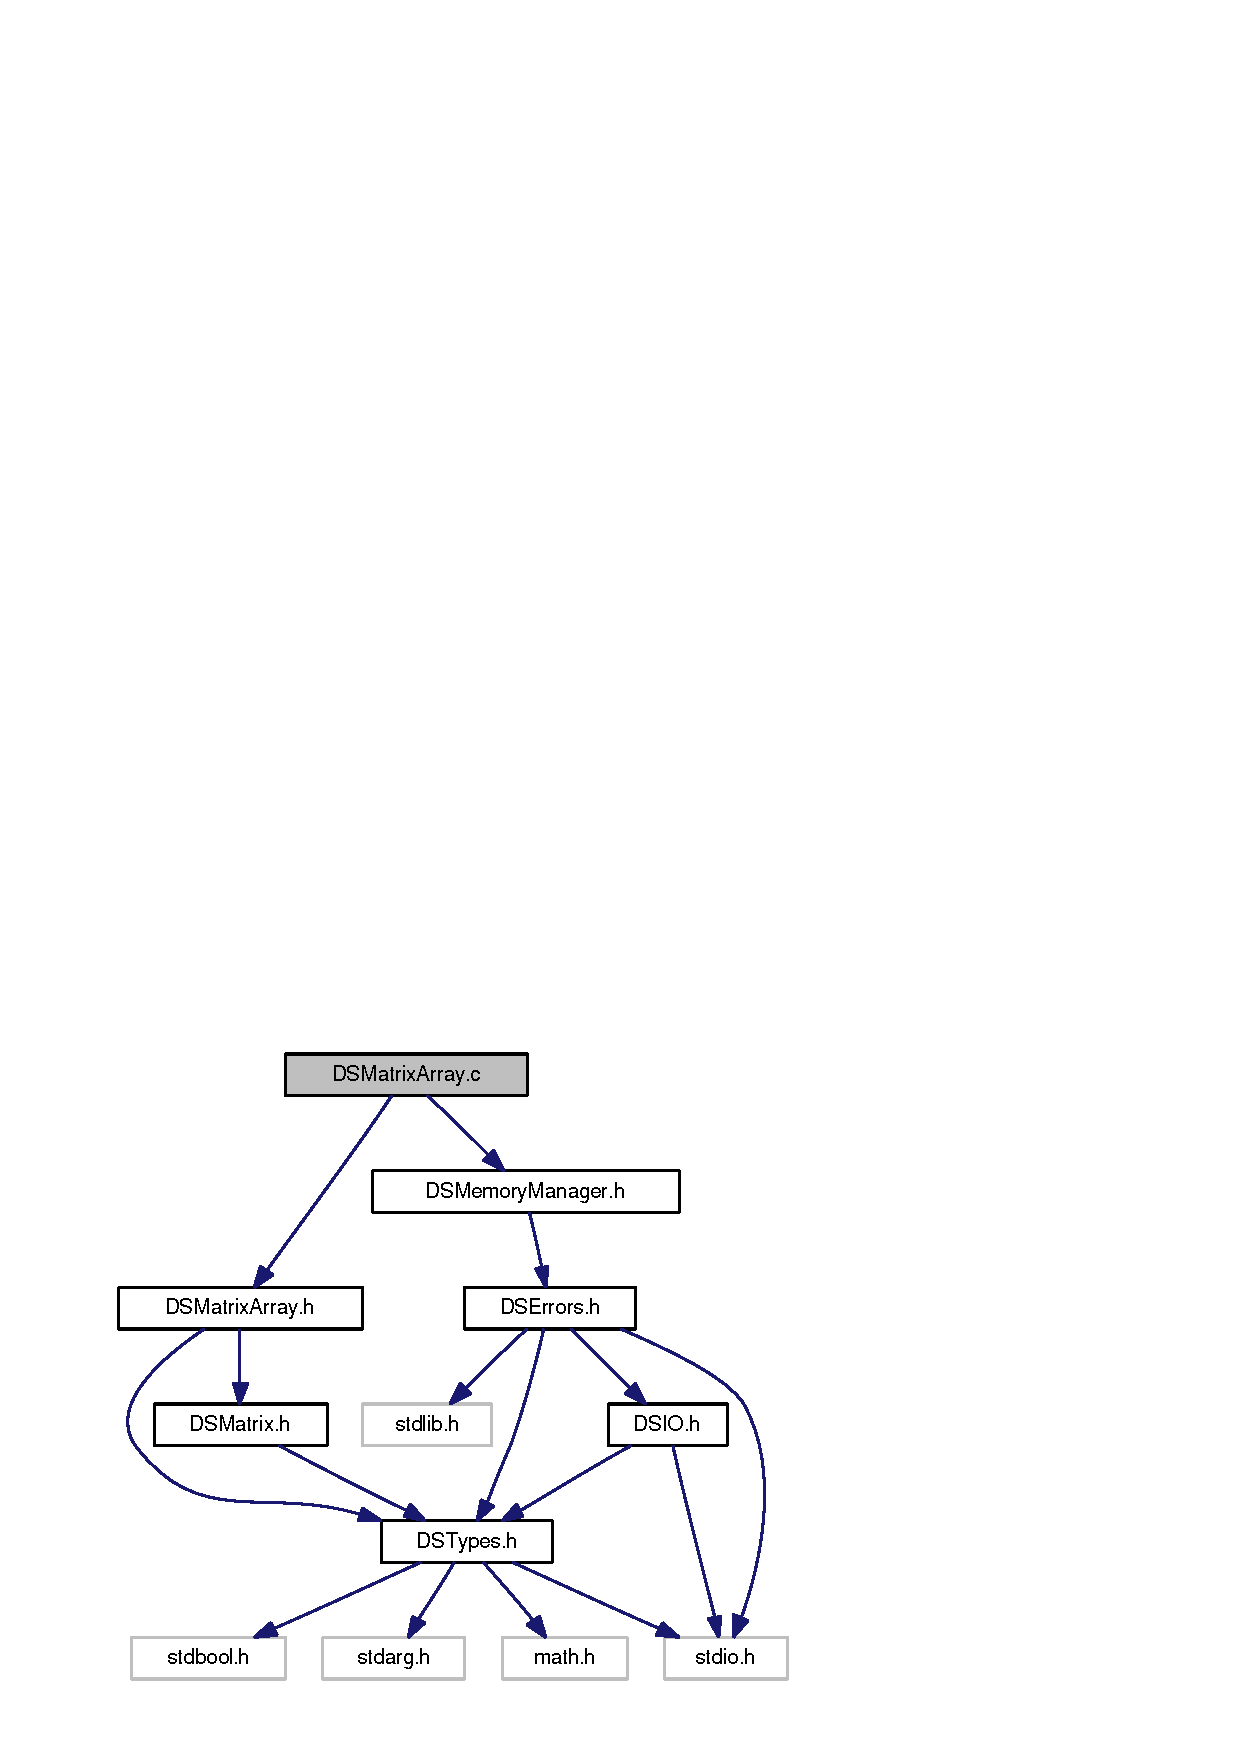
\includegraphics[width=193pt]{_d_s_matrix_array_8c__incl}
\end{center}
\end{figure}
\subsection*{Functions}
\begin{DoxyCompactItemize}
\item 
\hyperlink{struct_d_s_matrix_array}{DSMatrixArray} $\ast$ \hyperlink{_d_s_matrix_array_8c_ac28a8d64f99862378acc435e54c91c53}{DSMatrixArrayAlloc} (void)
\begin{DoxyCompactList}\small\item\em Memory allocation for a \hyperlink{struct_d_s_matrix_array}{DSMatrixArray}. \item\end{DoxyCompactList}\item 
\hyperlink{struct_d_s_matrix_array}{DSMatrixArray} $\ast$ \hyperlink{_d_s_matrix_array_8c_a694f4a21842a5e5bda0f4bdcb2e56626}{DSMatrixArrayCopy} (const \hyperlink{struct_d_s_matrix_array}{DSMatrixArray} $\ast$array)
\begin{DoxyCompactList}\small\item\em Copies a \hyperlink{struct_d_s_matrix_array}{DSMatrixArray}. \item\end{DoxyCompactList}\item 
void \hyperlink{_d_s_matrix_array_8c_a99f7d3e74613f43f22d8faa4bed25d1a}{DSMatrixArrayFree} (\hyperlink{struct_d_s_matrix_array}{DSMatrixArray} $\ast$array)
\begin{DoxyCompactList}\small\item\em Freeing memory for \hyperlink{struct_d_s_matrix_array}{DSMatrixArray}. \item\end{DoxyCompactList}\item 
\hyperlink{struct_d_s_matrix}{DSMatrix} $\ast$ \hyperlink{_d_s_matrix_array_8c_a4d9a430514e9384eea4a35ca826717c1}{DSMatrixArrayMatrix} (const \hyperlink{struct_d_s_matrix_array}{DSMatrixArray} $\ast$array, const DSUInteger index)
\begin{DoxyCompactList}\small\item\em Function to access a matrix in the \hyperlink{struct_d_s_matrix_array}{DSMatrixArray}. \item\end{DoxyCompactList}\item 
void \hyperlink{_d_s_matrix_array_8c_a91dd77e0cd7cff2173b6bfce9b9e7f4f}{DSMatrixArrayAddMatrix} (\hyperlink{struct_d_s_matrix_array}{DSMatrixArray} $\ast$array, const \hyperlink{struct_d_s_matrix}{DSMatrix} $\ast$matrixToAdd)
\begin{DoxyCompactList}\small\item\em Function to add a new matrix to the \hyperlink{struct_d_s_matrix_array}{DSMatrixArray}. \item\end{DoxyCompactList}\item 
\hypertarget{_d_s_matrix_array_8c_a78218c70cec38b886d663ad05c7031cf}{
double {\bfseries DSMatrixArrayDoubleWithIndices} (const \hyperlink{struct_d_s_matrix_array}{DSMatrixArray} $\ast$array, const DSUInteger i, const DSUInteger j, const DSUInteger k)}
\label{_d_s_matrix_array_8c_a78218c70cec38b886d663ad05c7031cf}

\item 
\hypertarget{_d_s_matrix_array_8c_ad4998c91be723d705130e33c3f554e14}{
void {\bfseries DSMatrixArrayPrint} (const \hyperlink{struct_d_s_matrix_array}{DSMatrixArray} $\ast$array)}
\label{_d_s_matrix_array_8c_ad4998c91be723d705130e33c3f554e14}

\end{DoxyCompactItemize}


\subsection{Detailed Description}
Implementation file with functions for dealing with matrix arrays. Copyright (C) 2011 Jason Lomnitz.\par
\par


This file is part of the Design Space Toolbox V2 (C Library).

The Design Space Toolbox V2 is free software: you can redistribute it and/or modify it under the terms of the GNU General Public License as published by the Free Software Foundation, either version 3 of the License, or (at your option) any later version.

The Design Space Toolbox V2 is distributed in the hope that it will be useful, but WITHOUT ANY WARRANTY; without even the implied warranty of MERCHANTABILITY or FITNESS FOR A PARTICULAR PURPOSE. See the GNU General Public License for more details.

You should have received a copy of the GNU General Public License along with the Design Space Toolbox. If not, see $<$\href{http://www.gnu.org/licenses/}{\tt http://www.gnu.org/licenses/}$>$.

\begin{DoxyAuthor}{Author}
Jason Lomnitz. 
\end{DoxyAuthor}
\begin{DoxyDate}{Date}
2011 
\end{DoxyDate}


\subsection{Function Documentation}
\hypertarget{_d_s_matrix_array_8c_a91dd77e0cd7cff2173b6bfce9b9e7f4f}{
\index{DSMatrixArray.c@{DSMatrixArray.c}!DSMatrixArrayAddMatrix@{DSMatrixArrayAddMatrix}}
\index{DSMatrixArrayAddMatrix@{DSMatrixArrayAddMatrix}!DSMatrixArray.c@{DSMatrixArray.c}}
\subsubsection[{DSMatrixArrayAddMatrix}]{\setlength{\rightskip}{0pt plus 5cm}void DSMatrixArrayAddMatrix ({\bf DSMatrixArray} $\ast$ {\em array}, \/  const {\bf DSMatrix} $\ast$ {\em matrixToAdd})}}
\label{_d_s_matrix_array_8c_a91dd77e0cd7cff2173b6bfce9b9e7f4f}


Function to add a new matrix to the \hyperlink{struct_d_s_matrix_array}{DSMatrixArray}. 

This function is the standard mechanism to add a \hyperlink{struct_d_s_matrix}{DSMatrix} to a \hyperlink{struct_d_s_matrix_array}{DSMatrixArray}. This function allocates the necessary space in the internal C array, and adds the \hyperlink{struct_d_s_matrix}{DSMatrix} to the end of the array. Once added to the matrix array, the memory is managed by the matrix array and is freed upon calling DSMatrixArrayFree.


\begin{DoxyParams}{Parameters}
\item[{\em array}]The \hyperlink{struct_d_s_matrix_array}{DSMatrixArray} that will have a new matrix added. \item[{\em matrixToAdd}]The \hyperlink{struct_d_s_matrix}{DSMatrix} to be added to the matrix array. \end{DoxyParams}
\hypertarget{_d_s_matrix_array_8c_ac28a8d64f99862378acc435e54c91c53}{
\index{DSMatrixArray.c@{DSMatrixArray.c}!DSMatrixArrayAlloc@{DSMatrixArrayAlloc}}
\index{DSMatrixArrayAlloc@{DSMatrixArrayAlloc}!DSMatrixArray.c@{DSMatrixArray.c}}
\subsubsection[{DSMatrixArrayAlloc}]{\setlength{\rightskip}{0pt plus 5cm}{\bf DSMatrixArray}$\ast$ DSMatrixArrayAlloc (void)}}
\label{_d_s_matrix_array_8c_ac28a8d64f99862378acc435e54c91c53}


Memory allocation for a \hyperlink{struct_d_s_matrix_array}{DSMatrixArray}. 

Creates a new \hyperlink{struct_d_s_matrix_array}{DSMatrixArray} with no matrices. As matrices are added, the matrix array grows, therefore the matrix array is initialized to 0, with a NULL internal pointer and number of matrices set to 0.

\begin{DoxyReturn}{Returns}
If the matrix array was created, a new pointer to a \hyperlink{struct_d_s_matrix}{DSMatrix} is returned. Otherwise, NULL is returned. 
\end{DoxyReturn}
\hypertarget{_d_s_matrix_array_8c_a694f4a21842a5e5bda0f4bdcb2e56626}{
\index{DSMatrixArray.c@{DSMatrixArray.c}!DSMatrixArrayCopy@{DSMatrixArrayCopy}}
\index{DSMatrixArrayCopy@{DSMatrixArrayCopy}!DSMatrixArray.c@{DSMatrixArray.c}}
\subsubsection[{DSMatrixArrayCopy}]{\setlength{\rightskip}{0pt plus 5cm}{\bf DSMatrixArray}$\ast$ DSMatrixArrayCopy (const {\bf DSMatrixArray} $\ast$ {\em array})}}
\label{_d_s_matrix_array_8c_a694f4a21842a5e5bda0f4bdcb2e56626}


Copies a \hyperlink{struct_d_s_matrix_array}{DSMatrixArray}. 

Creates a new \hyperlink{struct_d_s_matrix_array}{DSMatrixArray} with the exact same data and contents as some other matrix array. The matrices in the new \hyperlink{struct_d_s_matrix_array}{DSMatrixArray} are copies of the matrices in the original matrix array.


\begin{DoxyParams}{Parameters}
\item[{\em array}]The \hyperlink{struct_d_s_matrix_array}{DSMatrixArray} to be copied.\end{DoxyParams}
\begin{DoxyReturn}{Returns}
If the copy was succesful, a pointer to a copy of the \hyperlink{struct_d_s_matrix_array}{DSMatrixArray} is returned. Otherwise, NULL is returned.
\end{DoxyReturn}
\begin{DoxySeeAlso}{See also}
\hyperlink{_d_s_matrix__gsl_8c_a6d0f0f74bdd85829ba07dd33f51cfa11}{DSMatrixCopy} 
\end{DoxySeeAlso}
\hypertarget{_d_s_matrix_array_8c_a99f7d3e74613f43f22d8faa4bed25d1a}{
\index{DSMatrixArray.c@{DSMatrixArray.c}!DSMatrixArrayFree@{DSMatrixArrayFree}}
\index{DSMatrixArrayFree@{DSMatrixArrayFree}!DSMatrixArray.c@{DSMatrixArray.c}}
\subsubsection[{DSMatrixArrayFree}]{\setlength{\rightskip}{0pt plus 5cm}void DSMatrixArrayFree ({\bf DSMatrixArray} $\ast$ {\em array})}}
\label{_d_s_matrix_array_8c_a99f7d3e74613f43f22d8faa4bed25d1a}


Freeing memory for \hyperlink{struct_d_s_matrix_array}{DSMatrixArray}. 

Frees the memory associated with a \hyperlink{struct_d_s_matrix_array}{DSMatrixArray} data type. This function is a wrapper for the necessary steps needed to free the internal structure of the \hyperlink{struct_d_s_matrix_array}{DSMatrixArray}, this includes calling DSMatrixFree for each of the contained matrices, freeing the internal pointer to the array of matrices, and the \hyperlink{struct_d_s_matrix_array}{DSMatrixArray} data type itself.


\begin{DoxyParams}{Parameters}
\item[{\em array}]The \hyperlink{struct_d_s_matrix_array}{DSMatrixArray} to be freed. \end{DoxyParams}
\hypertarget{_d_s_matrix_array_8c_a4d9a430514e9384eea4a35ca826717c1}{
\index{DSMatrixArray.c@{DSMatrixArray.c}!DSMatrixArrayMatrix@{DSMatrixArrayMatrix}}
\index{DSMatrixArrayMatrix@{DSMatrixArrayMatrix}!DSMatrixArray.c@{DSMatrixArray.c}}
\subsubsection[{DSMatrixArrayMatrix}]{\setlength{\rightskip}{0pt plus 5cm}{\bf DSMatrix}$\ast$ DSMatrixArrayMatrix (const {\bf DSMatrixArray} $\ast$ {\em array}, \/  const DSUInteger {\em index})}}
\label{_d_s_matrix_array_8c_a4d9a430514e9384eea4a35ca826717c1}


Function to access a matrix in the \hyperlink{struct_d_s_matrix_array}{DSMatrixArray}. 

This accessor function returns the \hyperlink{struct_d_s_matrix}{DSMatrix} at the specified index of the \hyperlink{struct_d_s_matrix_array}{DSMatrixArray}. This function is the basic accessor function, and should always be used to access a matrix in a \hyperlink{struct_d_s_matrix_array}{DSMatrixArray}.


\begin{DoxyParams}{Parameters}
\item[{\em array}]The \hyperlink{struct_d_s_matrix_array}{DSMatrixArray} containing the matrix to be accessed. \item[{\em index}]The DSUInteger specifying the index in the C array of matrices contained in the \hyperlink{struct_d_s_matrix_array}{DSMatrixArray}.\end{DoxyParams}
\begin{DoxyReturn}{Returns}
If the \hyperlink{struct_d_s_matrix}{DSMatrix} at the specified index was found, the pointer to that matrix is returned. Otherwise, NULL is returned. 
\end{DoxyReturn}

\hypertarget{_d_s_matrix_array_8h}{
\section{DSMatrixArray.h File Reference}
\label{_d_s_matrix_array_8h}\index{DSMatrixArray.h@{DSMatrixArray.h}}
}


Header file with functions for dealing with matrix arrays.  


{\ttfamily \#include \char`\"{}DSTypes.h\char`\"{}}\par
{\ttfamily \#include \char`\"{}DSMatrix.h\char`\"{}}\par
Include dependency graph for DSMatrixArray.h:\nopagebreak
\begin{figure}[H]
\begin{center}
\leavevmode
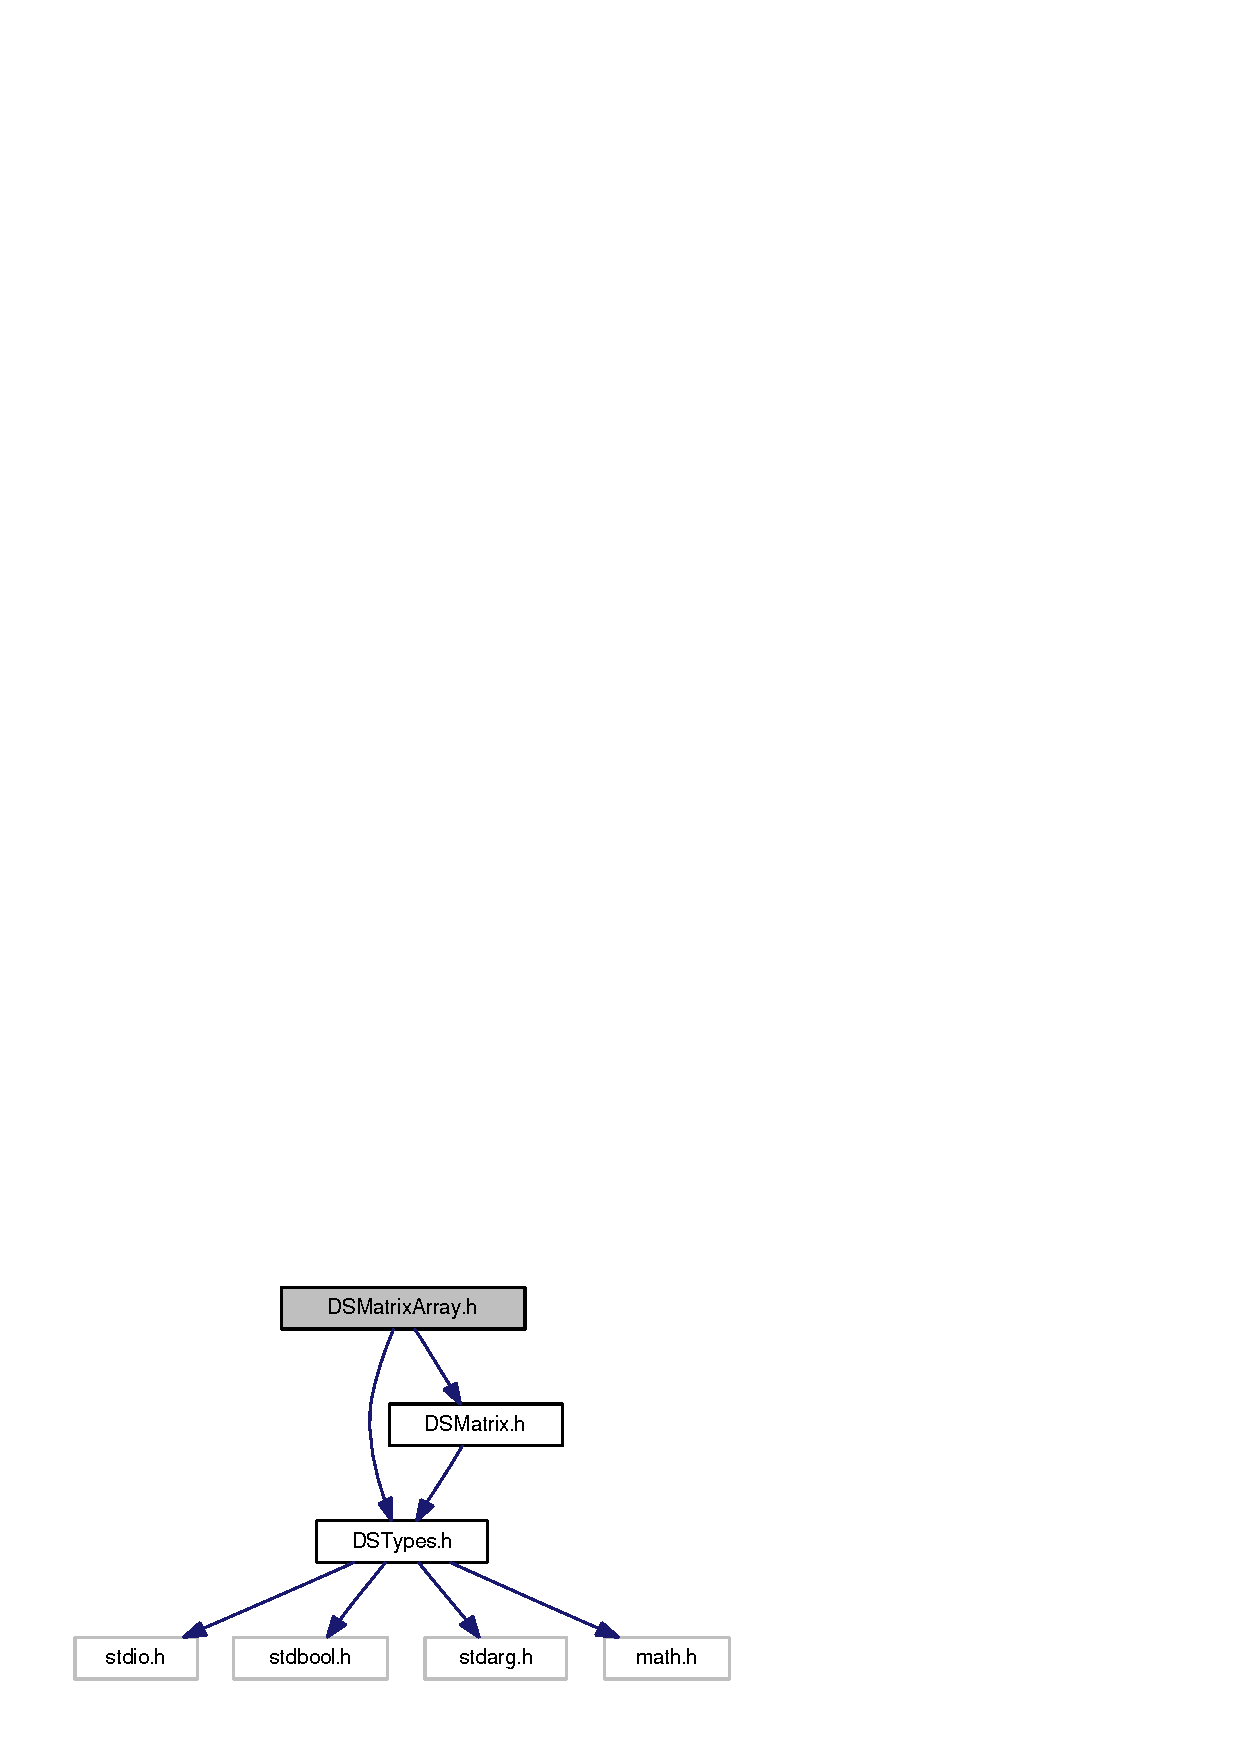
\includegraphics[width=175pt]{_d_s_matrix_array_8h__incl}
\end{center}
\end{figure}
This graph shows which files directly or indirectly include this file:\nopagebreak
\begin{figure}[H]
\begin{center}
\leavevmode
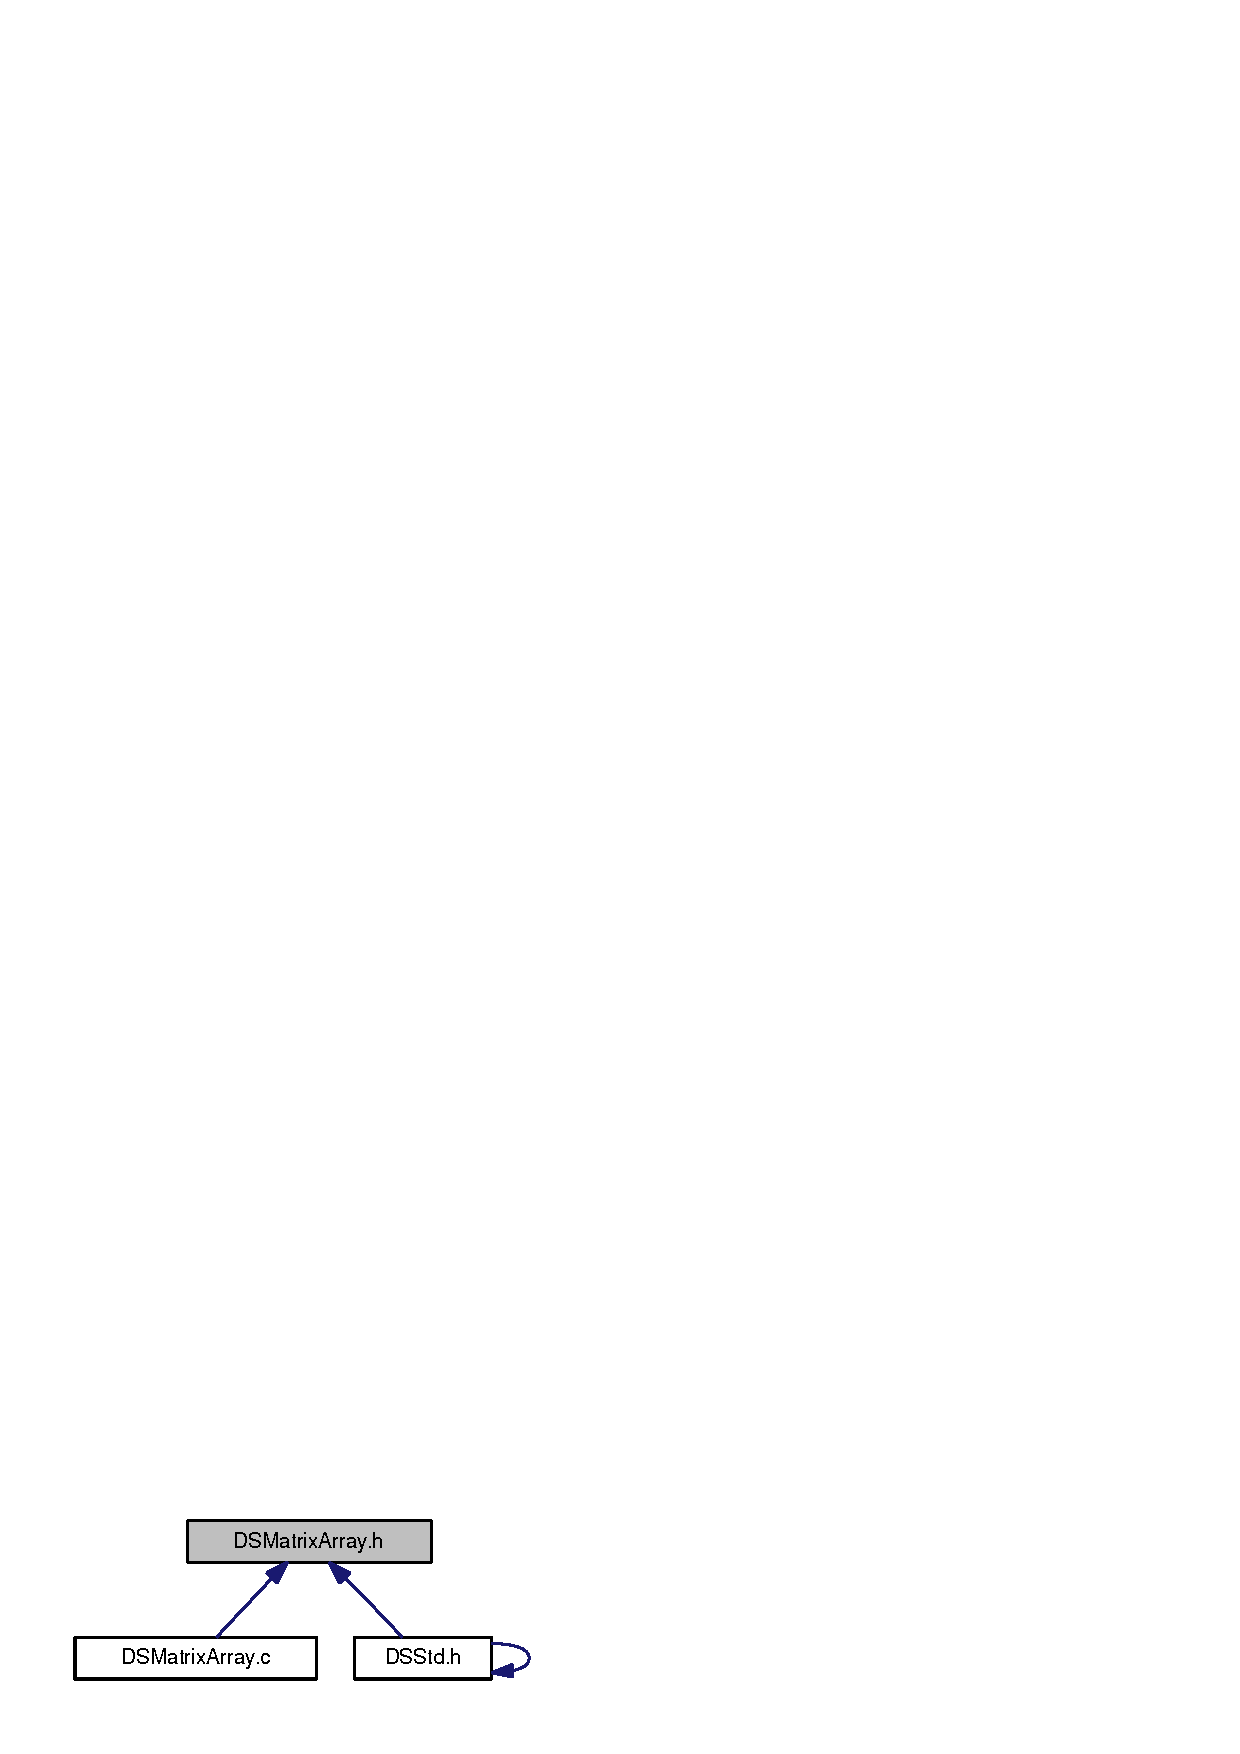
\includegraphics[width=127pt]{_d_s_matrix_array_8h__dep__incl}
\end{center}
\end{figure}
\subsection*{Defines}
\begin{DoxyCompactItemize}
\item 
\hypertarget{_d_s_matrix_array_8h_ae5ed293af50a4fe892a5064c6f026fd5}{
\#define \hyperlink{_d_s_matrix_array_8h_ae5ed293af50a4fe892a5064c6f026fd5}{DSMatrixArrayNumberOfMatrices}(x)~((x)-\/$>$numberOfMatrices)}
\label{_d_s_matrix_array_8h_ae5ed293af50a4fe892a5064c6f026fd5}

\begin{DoxyCompactList}\small\item\em Accessor function to retrieve number of matrices in the Matrix array. \item\end{DoxyCompactList}\item 
\hypertarget{_d_s_matrix_array_8h_ad12db3a5ec12ae7eb52f988b529b4a80}{
\#define \hyperlink{_d_s_matrix_array_8h_ad12db3a5ec12ae7eb52f988b529b4a80}{DSMatrixArrayInternalPointer}(x)~((x)-\/$>$matrices)}
\label{_d_s_matrix_array_8h_ad12db3a5ec12ae7eb52f988b529b4a80}

\begin{DoxyCompactList}\small\item\em Accessor function to retrieve the pointer to the C matrix array. \item\end{DoxyCompactList}\end{DoxyCompactItemize}
\subsection*{Functions}
\begin{DoxyCompactItemize}
\item 
\hyperlink{struct_d_s_matrix_array}{DSMatrixArray} $\ast$ \hyperlink{_d_s_matrix_array_8h_ac28a8d64f99862378acc435e54c91c53}{DSMatrixArrayAlloc} (void)
\begin{DoxyCompactList}\small\item\em Memory allocation for a \hyperlink{struct_d_s_matrix_array}{DSMatrixArray}. \item\end{DoxyCompactList}\item 
\hyperlink{struct_d_s_matrix_array}{DSMatrixArray} $\ast$ \hyperlink{_d_s_matrix_array_8h_a694f4a21842a5e5bda0f4bdcb2e56626}{DSMatrixArrayCopy} (const \hyperlink{struct_d_s_matrix_array}{DSMatrixArray} $\ast$array)
\begin{DoxyCompactList}\small\item\em Copies a \hyperlink{struct_d_s_matrix_array}{DSMatrixArray}. \item\end{DoxyCompactList}\item 
void \hyperlink{_d_s_matrix_array_8h_a99f7d3e74613f43f22d8faa4bed25d1a}{DSMatrixArrayFree} (\hyperlink{struct_d_s_matrix_array}{DSMatrixArray} $\ast$array)
\begin{DoxyCompactList}\small\item\em Freeing memory for \hyperlink{struct_d_s_matrix_array}{DSMatrixArray}. \item\end{DoxyCompactList}\item 
\hyperlink{struct_d_s_matrix}{DSMatrix} $\ast$ \hyperlink{_d_s_matrix_array_8h_a4d9a430514e9384eea4a35ca826717c1}{DSMatrixArrayMatrix} (const \hyperlink{struct_d_s_matrix_array}{DSMatrixArray} $\ast$array, const DSUInteger index)
\begin{DoxyCompactList}\small\item\em Function to access a matrix in the \hyperlink{struct_d_s_matrix_array}{DSMatrixArray}. \item\end{DoxyCompactList}\item 
void \hyperlink{_d_s_matrix_array_8h_a91dd77e0cd7cff2173b6bfce9b9e7f4f}{DSMatrixArrayAddMatrix} (\hyperlink{struct_d_s_matrix_array}{DSMatrixArray} $\ast$array, const \hyperlink{struct_d_s_matrix}{DSMatrix} $\ast$matrixToAdd)
\begin{DoxyCompactList}\small\item\em Function to add a new matrix to the \hyperlink{struct_d_s_matrix_array}{DSMatrixArray}. \item\end{DoxyCompactList}\item 
\hypertarget{_d_s_matrix_array_8h_a78218c70cec38b886d663ad05c7031cf}{
double {\bfseries DSMatrixArrayDoubleWithIndices} (const \hyperlink{struct_d_s_matrix_array}{DSMatrixArray} $\ast$array, const DSUInteger i, const DSUInteger j, const DSUInteger k)}
\label{_d_s_matrix_array_8h_a78218c70cec38b886d663ad05c7031cf}

\item 
\hypertarget{_d_s_matrix_array_8h_ad4998c91be723d705130e33c3f554e14}{
void {\bfseries DSMatrixArrayPrint} (const \hyperlink{struct_d_s_matrix_array}{DSMatrixArray} $\ast$array)}
\label{_d_s_matrix_array_8h_ad4998c91be723d705130e33c3f554e14}

\end{DoxyCompactItemize}


\subsection{Detailed Description}
Header file with functions for dealing with matrix arrays. Copyright (C) 2011 Jason Lomnitz.\par
\par


This file is part of the Design Space Toolbox V2 (C Library).

The Design Space Toolbox V2 is free software: you can redistribute it and/or modify it under the terms of the GNU General Public License as published by the Free Software Foundation, either version 3 of the License, or (at your option) any later version.

The Design Space Toolbox V2 is distributed in the hope that it will be useful, but WITHOUT ANY WARRANTY; without even the implied warranty of MERCHANTABILITY or FITNESS FOR A PARTICULAR PURPOSE. See the GNU General Public License for more details.

You should have received a copy of the GNU General Public License along with the Design Space Toolbox. If not, see $<$\href{http://www.gnu.org/licenses/}{\tt http://www.gnu.org/licenses/}$>$.

\begin{DoxyAuthor}{Author}
Jason Lomnitz. 
\end{DoxyAuthor}
\begin{DoxyDate}{Date}
2011 
\end{DoxyDate}


\subsection{Function Documentation}
\hypertarget{_d_s_matrix_array_8h_a91dd77e0cd7cff2173b6bfce9b9e7f4f}{
\index{DSMatrixArray.h@{DSMatrixArray.h}!DSMatrixArrayAddMatrix@{DSMatrixArrayAddMatrix}}
\index{DSMatrixArrayAddMatrix@{DSMatrixArrayAddMatrix}!DSMatrixArray.h@{DSMatrixArray.h}}
\subsubsection[{DSMatrixArrayAddMatrix}]{\setlength{\rightskip}{0pt plus 5cm}void DSMatrixArrayAddMatrix ({\bf DSMatrixArray} $\ast$ {\em array}, \/  const {\bf DSMatrix} $\ast$ {\em matrixToAdd})}}
\label{_d_s_matrix_array_8h_a91dd77e0cd7cff2173b6bfce9b9e7f4f}


Function to add a new matrix to the \hyperlink{struct_d_s_matrix_array}{DSMatrixArray}. 

This function is the standard mechanism to add a \hyperlink{struct_d_s_matrix}{DSMatrix} to a \hyperlink{struct_d_s_matrix_array}{DSMatrixArray}. This function allocates the necessary space in the internal C array, and adds the \hyperlink{struct_d_s_matrix}{DSMatrix} to the end of the array. Once added to the matrix array, the memory is managed by the matrix array and is freed upon calling DSMatrixArrayFree.


\begin{DoxyParams}{Parameters}
\item[{\em array}]The \hyperlink{struct_d_s_matrix_array}{DSMatrixArray} that will have a new matrix added. \item[{\em matrixToAdd}]The \hyperlink{struct_d_s_matrix}{DSMatrix} to be added to the matrix array. \end{DoxyParams}
\hypertarget{_d_s_matrix_array_8h_ac28a8d64f99862378acc435e54c91c53}{
\index{DSMatrixArray.h@{DSMatrixArray.h}!DSMatrixArrayAlloc@{DSMatrixArrayAlloc}}
\index{DSMatrixArrayAlloc@{DSMatrixArrayAlloc}!DSMatrixArray.h@{DSMatrixArray.h}}
\subsubsection[{DSMatrixArrayAlloc}]{\setlength{\rightskip}{0pt plus 5cm}{\bf DSMatrixArray}$\ast$ DSMatrixArrayAlloc (void)}}
\label{_d_s_matrix_array_8h_ac28a8d64f99862378acc435e54c91c53}


Memory allocation for a \hyperlink{struct_d_s_matrix_array}{DSMatrixArray}. 

Creates a new \hyperlink{struct_d_s_matrix_array}{DSMatrixArray} with no matrices. As matrices are added, the matrix array grows, therefore the matrix array is initialized to 0, with a NULL internal pointer and number of matrices set to 0.

\begin{DoxyReturn}{Returns}
If the matrix array was created, a new pointer to a \hyperlink{struct_d_s_matrix}{DSMatrix} is returned. Otherwise, NULL is returned. 
\end{DoxyReturn}
\hypertarget{_d_s_matrix_array_8h_a694f4a21842a5e5bda0f4bdcb2e56626}{
\index{DSMatrixArray.h@{DSMatrixArray.h}!DSMatrixArrayCopy@{DSMatrixArrayCopy}}
\index{DSMatrixArrayCopy@{DSMatrixArrayCopy}!DSMatrixArray.h@{DSMatrixArray.h}}
\subsubsection[{DSMatrixArrayCopy}]{\setlength{\rightskip}{0pt plus 5cm}{\bf DSMatrixArray}$\ast$ DSMatrixArrayCopy (const {\bf DSMatrixArray} $\ast$ {\em array})}}
\label{_d_s_matrix_array_8h_a694f4a21842a5e5bda0f4bdcb2e56626}


Copies a \hyperlink{struct_d_s_matrix_array}{DSMatrixArray}. 

Creates a new \hyperlink{struct_d_s_matrix_array}{DSMatrixArray} with the exact same data and contents as some other matrix array. The matrices in the new \hyperlink{struct_d_s_matrix_array}{DSMatrixArray} are copies of the matrices in the original matrix array.


\begin{DoxyParams}{Parameters}
\item[{\em array}]The \hyperlink{struct_d_s_matrix_array}{DSMatrixArray} to be copied.\end{DoxyParams}
\begin{DoxyReturn}{Returns}
If the copy was succesful, a pointer to a copy of the \hyperlink{struct_d_s_matrix_array}{DSMatrixArray} is returned. Otherwise, NULL is returned.
\end{DoxyReturn}
\begin{DoxySeeAlso}{See also}
\hyperlink{_d_s_matrix__gsl_8c_a6d0f0f74bdd85829ba07dd33f51cfa11}{DSMatrixCopy} 
\end{DoxySeeAlso}
\hypertarget{_d_s_matrix_array_8h_a99f7d3e74613f43f22d8faa4bed25d1a}{
\index{DSMatrixArray.h@{DSMatrixArray.h}!DSMatrixArrayFree@{DSMatrixArrayFree}}
\index{DSMatrixArrayFree@{DSMatrixArrayFree}!DSMatrixArray.h@{DSMatrixArray.h}}
\subsubsection[{DSMatrixArrayFree}]{\setlength{\rightskip}{0pt plus 5cm}void DSMatrixArrayFree ({\bf DSMatrixArray} $\ast$ {\em array})}}
\label{_d_s_matrix_array_8h_a99f7d3e74613f43f22d8faa4bed25d1a}


Freeing memory for \hyperlink{struct_d_s_matrix_array}{DSMatrixArray}. 

Frees the memory associated with a \hyperlink{struct_d_s_matrix_array}{DSMatrixArray} data type. This function is a wrapper for the necessary steps needed to free the internal structure of the \hyperlink{struct_d_s_matrix_array}{DSMatrixArray}, this includes calling DSMatrixFree for each of the contained matrices, freeing the internal pointer to the array of matrices, and the \hyperlink{struct_d_s_matrix_array}{DSMatrixArray} data type itself.


\begin{DoxyParams}{Parameters}
\item[{\em array}]The \hyperlink{struct_d_s_matrix_array}{DSMatrixArray} to be freed. \end{DoxyParams}
\hypertarget{_d_s_matrix_array_8h_a4d9a430514e9384eea4a35ca826717c1}{
\index{DSMatrixArray.h@{DSMatrixArray.h}!DSMatrixArrayMatrix@{DSMatrixArrayMatrix}}
\index{DSMatrixArrayMatrix@{DSMatrixArrayMatrix}!DSMatrixArray.h@{DSMatrixArray.h}}
\subsubsection[{DSMatrixArrayMatrix}]{\setlength{\rightskip}{0pt plus 5cm}{\bf DSMatrix}$\ast$ DSMatrixArrayMatrix (const {\bf DSMatrixArray} $\ast$ {\em array}, \/  const DSUInteger {\em index})}}
\label{_d_s_matrix_array_8h_a4d9a430514e9384eea4a35ca826717c1}


Function to access a matrix in the \hyperlink{struct_d_s_matrix_array}{DSMatrixArray}. 

This accessor function returns the \hyperlink{struct_d_s_matrix}{DSMatrix} at the specified index of the \hyperlink{struct_d_s_matrix_array}{DSMatrixArray}. This function is the basic accessor function, and should always be used to access a matrix in a \hyperlink{struct_d_s_matrix_array}{DSMatrixArray}.


\begin{DoxyParams}{Parameters}
\item[{\em array}]The \hyperlink{struct_d_s_matrix_array}{DSMatrixArray} containing the matrix to be accessed. \item[{\em index}]The DSUInteger specifying the index in the C array of matrices contained in the \hyperlink{struct_d_s_matrix_array}{DSMatrixArray}.\end{DoxyParams}
\begin{DoxyReturn}{Returns}
If the \hyperlink{struct_d_s_matrix}{DSMatrix} at the specified index was found, the pointer to that matrix is returned. Otherwise, NULL is returned. 
\end{DoxyReturn}

\hypertarget{_d_s_matrix_tokenizer_8c}{
\section{DSMatrixTokenizer.c File Reference}
\label{_d_s_matrix_tokenizer_8c}\index{DSMatrixTokenizer.c@{DSMatrixTokenizer.c}}
}


Implementation file with functions for tokenizing with matrices.  


{\ttfamily \#include $<$stdio.h$>$}\par
{\ttfamily \#include \char`\"{}DSMatrixTokenizer.h\char`\"{}}\par
Include dependency graph for DSMatrixTokenizer.c:\subsection*{Functions}
\begin{DoxyCompactItemize}
\item 
\hypertarget{_d_s_matrix_tokenizer_8c_ae96d345bf776c1f541097e208df35238}{
struct \hyperlink{structmatrix__token}{matrix\_\-token} $\ast$ {\bfseries DSMatrixTokenAlloc} ()}
\label{_d_s_matrix_tokenizer_8c_ae96d345bf776c1f541097e208df35238}

\item 
\hypertarget{_d_s_matrix_tokenizer_8c_ac248874858bfc45bb57d74f008a79e32}{
void {\bfseries DSMatrixTokenFree} (struct \hyperlink{structmatrix__token}{matrix\_\-token} $\ast$root)}
\label{_d_s_matrix_tokenizer_8c_ac248874858bfc45bb57d74f008a79e32}

\end{DoxyCompactItemize}


\subsection{Detailed Description}
Implementation file with functions for tokenizing with matrices. Copyright (C) 2011 Jason Lomnitz.\par
\par


This file is part of the Design Space Toolbox V2 (C Library).

The Design Space Toolbox V2 is free software: you can redistribute it and/or modify it under the terms of the GNU General Public License as published by the Free Software Foundation, either version 3 of the License, or (at your option) any later version.

The Design Space Toolbox V2 is distributed in the hope that it will be useful, but WITHOUT ANY WARRANTY; without even the implied warranty of MERCHANTABILITY or FITNESS FOR A PARTICULAR PURPOSE. See the GNU General Public License for more details.

You should have received a copy of the GNU General Public License along with the Design Space Toolbox. If not, see $<$\href{http://www.gnu.org/licenses/}{\tt http://www.gnu.org/licenses/}$>$.

\begin{DoxyAuthor}{Author}
Jason Lomnitz. 
\end{DoxyAuthor}
\begin{DoxyDate}{Date}
2011 
\end{DoxyDate}

\hypertarget{_d_s_matrix_tokenizer_8h}{
\section{DSMatrixTokenizer.h File Reference}
\label{_d_s_matrix_tokenizer_8h}\index{DSMatrixTokenizer.h@{DSMatrixTokenizer.h}}
}


Header file with functions for tokenizing matrices.  


{\ttfamily \#include \char`\"{}DSTypes.h\char`\"{}}\par
{\ttfamily \#include \char`\"{}DSErrors.h\char`\"{}}\par
{\ttfamily \#include \char`\"{}DSMemoryManager.h\char`\"{}}\par
Include dependency graph for DSMatrixTokenizer.h:This graph shows which files directly or indirectly include this file:\subsection*{Data Structures}
\begin{DoxyCompactItemize}
\item 
struct \hyperlink{structmatrix__token}{matrix\_\-token}
\end{DoxyCompactItemize}
\subsection*{Defines}
\begin{DoxyCompactItemize}
\item 
\hypertarget{_d_s_matrix_tokenizer_8h_afb9241dfd12d62583187267ce880dbc4}{
\#define \hyperlink{_d_s_matrix_tokenizer_8h_afb9241dfd12d62583187267ce880dbc4}{DS\_\-MATRIX\_\-TOKEN\_\-START}~0}
\label{_d_s_matrix_tokenizer_8h_afb9241dfd12d62583187267ce880dbc4}

\begin{DoxyCompactList}\small\item\em Token indicating the start of a tokenization. \item\end{DoxyCompactList}\item 
\hypertarget{_d_s_matrix_tokenizer_8h_a58952e47f0dfb776a9df004d3cb7f678}{
\#define \hyperlink{_d_s_matrix_tokenizer_8h_a58952e47f0dfb776a9df004d3cb7f678}{DS\_\-MATRIX\_\-TOKEN\_\-DOUBLE}~1}
\label{_d_s_matrix_tokenizer_8h_a58952e47f0dfb776a9df004d3cb7f678}

\begin{DoxyCompactList}\small\item\em Token indicating a numerical value. \item\end{DoxyCompactList}\item 
\hypertarget{_d_s_matrix_tokenizer_8h_aa92efbc0ffbfe186b8976262301ee6f2}{
\#define \hyperlink{_d_s_matrix_tokenizer_8h_aa92efbc0ffbfe186b8976262301ee6f2}{DS\_\-MATRIX\_\-TOKEN\_\-NEWLINE}~2}
\label{_d_s_matrix_tokenizer_8h_aa92efbc0ffbfe186b8976262301ee6f2}

\begin{DoxyCompactList}\small\item\em Token indicating a newline, indicative of a new row. \item\end{DoxyCompactList}\item 
\hypertarget{_d_s_matrix_tokenizer_8h_a6b45c2b28004946c0bc42cb88f381544}{
\#define \hyperlink{_d_s_matrix_tokenizer_8h_a6b45c2b28004946c0bc42cb88f381544}{DS\_\-MATRIX\_\-TOKEN\_\-ERROR}~3}
\label{_d_s_matrix_tokenizer_8h_a6b45c2b28004946c0bc42cb88f381544}

\begin{DoxyCompactList}\small\item\em Token indicating an error during tokenization. \item\end{DoxyCompactList}\item 
\hypertarget{_d_s_matrix_tokenizer_8h_afb1e04e4d142f486e0a342147a08cce7}{
\#define {\bfseries DSMatrixTokenNext}(x)~((x)-\/$>$next)}
\label{_d_s_matrix_tokenizer_8h_afb1e04e4d142f486e0a342147a08cce7}

\item 
\hypertarget{_d_s_matrix_tokenizer_8h_acbe81d77c75f0551b0607c83fbe53051}{
\#define {\bfseries DSMatrixTokenValue}(x)~((x)-\/$>$value)}
\label{_d_s_matrix_tokenizer_8h_acbe81d77c75f0551b0607c83fbe53051}

\item 
\hypertarget{_d_s_matrix_tokenizer_8h_a38bb235b766f70ef023459de2469cc07}{
\#define {\bfseries DSMatrixTokenType}(x)~((x)-\/$>$token)}
\label{_d_s_matrix_tokenizer_8h_a38bb235b766f70ef023459de2469cc07}

\item 
\hypertarget{_d_s_matrix_tokenizer_8h_a58ef09840dc2ecfbef159214fb73d652}{
\#define {\bfseries DSMatrixTokenRow}(x)~((x)-\/$>$row)}
\label{_d_s_matrix_tokenizer_8h_a58ef09840dc2ecfbef159214fb73d652}

\item 
\hypertarget{_d_s_matrix_tokenizer_8h_ae94916baa4dde2b2a56367e4eaa03c84}{
\#define {\bfseries DSMatrixTokenColumn}(x)~((x)-\/$>$column)}
\label{_d_s_matrix_tokenizer_8h_ae94916baa4dde2b2a56367e4eaa03c84}

\item 
\hypertarget{_d_s_matrix_tokenizer_8h_aac1e81659e69123069ebff2c6b9204e0}{
\#define {\bfseries DSMatrixTokenSetNext}(x, y)~((x)-\/$>$next = (y))}
\label{_d_s_matrix_tokenizer_8h_aac1e81659e69123069ebff2c6b9204e0}

\item 
\hypertarget{_d_s_matrix_tokenizer_8h_a7cadfcd946824627e0529d03562f955a}{
\#define {\bfseries DSMatrixTokenSetValue}(x, y)~((x)-\/$>$value = (y))}
\label{_d_s_matrix_tokenizer_8h_a7cadfcd946824627e0529d03562f955a}

\item 
\hypertarget{_d_s_matrix_tokenizer_8h_a45bdcbfaea99011b561aa71d9ee1d14a}{
\#define {\bfseries DSMatrixTokenSetType}(x, y)~((x)-\/$>$token = (y))}
\label{_d_s_matrix_tokenizer_8h_a45bdcbfaea99011b561aa71d9ee1d14a}

\item 
\hypertarget{_d_s_matrix_tokenizer_8h_a9946a83268d09eca85ff13eef15e0aca}{
\#define {\bfseries DSMatrixTokenSetRow}(x, y)~((x)-\/$>$row = (y))}
\label{_d_s_matrix_tokenizer_8h_a9946a83268d09eca85ff13eef15e0aca}

\item 
\hypertarget{_d_s_matrix_tokenizer_8h_ae3f4ee027ec95665318606751bcb9268}{
\#define {\bfseries DSMatrixTokenSetColumn}(x, y)~((x)-\/$>$column = (y))}
\label{_d_s_matrix_tokenizer_8h_ae3f4ee027ec95665318606751bcb9268}

\end{DoxyCompactItemize}
\subsection*{Functions}
\begin{DoxyCompactItemize}
\item 
\hypertarget{_d_s_matrix_tokenizer_8h_ae96d345bf776c1f541097e208df35238}{
struct \hyperlink{structmatrix__token}{matrix\_\-token} $\ast$ {\bfseries DSMatrixTokenAlloc} ()}
\label{_d_s_matrix_tokenizer_8h_ae96d345bf776c1f541097e208df35238}

\item 
\hypertarget{_d_s_matrix_tokenizer_8h_ac248874858bfc45bb57d74f008a79e32}{
void {\bfseries DSMatrixTokenFree} (struct \hyperlink{structmatrix__token}{matrix\_\-token} $\ast$root)}
\label{_d_s_matrix_tokenizer_8h_ac248874858bfc45bb57d74f008a79e32}

\item 
\hypertarget{_d_s_matrix_tokenizer_8h_ac946564137ea5b66ee2f08e5867c8c43}{
struct \hyperlink{structmatrix__token}{matrix\_\-token} $\ast$ {\bfseries DSMatrixTokenizeString} (const char $\ast$string)}
\label{_d_s_matrix_tokenizer_8h_ac946564137ea5b66ee2f08e5867c8c43}

\end{DoxyCompactItemize}


\subsection{Detailed Description}
Header file with functions for tokenizing matrices. This header file specifies the data structure relating to the tokenization of an input string to be parsed as a matrix, as well as all the functions necessary to tokenize it. This file is a provate file, and therefore its contents will be invisible to the public API. As such, it is not necessary to place the C++ compatability decleration.

Copyright (C) 2011 Jason Lomnitz.\par
\par


This file is part of the Design Space Toolbox V2 (C Library).

The Design Space Toolbox V2 is free software: you can redistribute it and/or modify it under the terms of the GNU General Public License as published by the Free Software Foundation, either version 3 of the License, or (at your option) any later version.

The Design Space Toolbox V2 is distributed in the hope that it will be useful, but WITHOUT ANY WARRANTY; without even the implied warranty of MERCHANTABILITY or FITNESS FOR A PARTICULAR PURPOSE. See the GNU General Public License for more details.

You should have received a copy of the GNU General Public License along with the Design Space Toolbox. If not, see $<$\href{http://www.gnu.org/licenses/}{\tt http://www.gnu.org/licenses/}$>$.

\begin{DoxyAuthor}{Author}
Jason Lomnitz. 
\end{DoxyAuthor}
\begin{DoxyDate}{Date}
2011
\end{DoxyDate}
This header file specifies the data structure relating to the tokenization of an input string to be parsed as a matrix, as well as all the functions necessary to tokenize it. This file is a private file, and therefore its contents will be invisible to the public API. Therefore, it is unnecessary to place the C++ compatability declerations.

Copyright (C) 2011 Jason Lomnitz.\par
\par


This file is part of the Design Space Toolbox V2 (C Library).

The Design Space Toolbox V2 is free software: you can redistribute it and/or modify it under the terms of the GNU General Public License as published by the Free Software Foundation, either version 3 of the License, or (at your option) any later version.

The Design Space Toolbox V2 is distributed in the hope that it will be useful, but WITHOUT ANY WARRANTY; without even the implied warranty of MERCHANTABILITY or FITNESS FOR A PARTICULAR PURPOSE. See the GNU General Public License for more details.

You should have received a copy of the GNU General Public License along with the Design Space Toolbox. If not, see $<$\href{http://www.gnu.org/licenses/}{\tt http://www.gnu.org/licenses/}$>$.

\begin{DoxyAuthor}{Author}
Jason Lomnitz. 
\end{DoxyAuthor}
\begin{DoxyDate}{Date}
2011 
\end{DoxyDate}

\hypertarget{_d_s_matrix_tokenizer_lex_8c}{
\section{DSMatrixTokenizerLex.c File Reference}
\label{_d_s_matrix_tokenizer_lex_8c}\index{DSMatrixTokenizerLex.c@{DSMatrixTokenizerLex.c}}
}


Implementation file with functions for tokenizing matrices, generated by flex.  


{\ttfamily \#include $<$stdio.h$>$}\par
{\ttfamily \#include $<$string.h$>$}\par
{\ttfamily \#include $<$errno.h$>$}\par
{\ttfamily \#include $<$stdlib.h$>$}\par
{\ttfamily \#include \char`\"{}DSTypes.h\char`\"{}}\par
{\ttfamily \#include \char`\"{}DSMemoryManager.h\char`\"{}}\par
{\ttfamily \#include \char`\"{}DSMatrix.h\char`\"{}}\par
{\ttfamily \#include \char`\"{}DSMatrixTokenizer.h\char`\"{}}\par
{\ttfamily \#include $<$unistd.h$>$}\par
Include dependency graph for DSMatrixTokenizerLex.c:\subsection*{Data Structures}
\begin{DoxyCompactItemize}
\item 
struct \hyperlink{structyy__buffer__state}{yy\_\-buffer\_\-state}
\item 
struct \hyperlink{structyy__trans__info}{yy\_\-trans\_\-info}
\item 
struct \hyperlink{structyyguts__t}{yyguts\_\-t}
\end{DoxyCompactItemize}
\subsection*{Defines}
\begin{DoxyCompactItemize}
\item 
\hypertarget{_d_s_matrix_tokenizer_lex_8c_a1ae16e642a197fa4948998525813c6f5}{
\#define {\bfseries YY\_\-INT\_\-ALIGNED}~short int}
\label{_d_s_matrix_tokenizer_lex_8c_a1ae16e642a197fa4948998525813c6f5}

\item 
\hypertarget{_d_s_matrix_tokenizer_lex_8c_a3c3d1ef92e93b0bc81d7760a73d5c3b6}{
\#define {\bfseries FLEX\_\-SCANNER}}
\label{_d_s_matrix_tokenizer_lex_8c_a3c3d1ef92e93b0bc81d7760a73d5c3b6}

\item 
\hypertarget{_d_s_matrix_tokenizer_lex_8c_a243ca1d30872935faf05ea5118ed6fdc}{
\#define {\bfseries YY\_\-FLEX\_\-MAJOR\_\-VERSION}~2}
\label{_d_s_matrix_tokenizer_lex_8c_a243ca1d30872935faf05ea5118ed6fdc}

\item 
\hypertarget{_d_s_matrix_tokenizer_lex_8c_a90f9d458829400869e47efb68a865677}{
\#define {\bfseries YY\_\-FLEX\_\-MINOR\_\-VERSION}~5}
\label{_d_s_matrix_tokenizer_lex_8c_a90f9d458829400869e47efb68a865677}

\item 
\hypertarget{_d_s_matrix_tokenizer_lex_8c_ac676bd06869180ea493e9b6d7c078dbb}{
\#define {\bfseries YY\_\-FLEX\_\-SUBMINOR\_\-VERSION}~35}
\label{_d_s_matrix_tokenizer_lex_8c_ac676bd06869180ea493e9b6d7c078dbb}

\item 
\hypertarget{_d_s_matrix_tokenizer_lex_8c_ad4e9955955b27624963643eac448118a}{
\#define {\bfseries INT16\_\-MIN}~(-\/32767-\/1)}
\label{_d_s_matrix_tokenizer_lex_8c_ad4e9955955b27624963643eac448118a}

\item 
\hypertarget{_d_s_matrix_tokenizer_lex_8c_a688eb21a22db27c2b2bd5836943cdcbe}{
\#define {\bfseries INT32\_\-MIN}~(-\/2147483647-\/1)}
\label{_d_s_matrix_tokenizer_lex_8c_a688eb21a22db27c2b2bd5836943cdcbe}

\item 
\hypertarget{_d_s_matrix_tokenizer_lex_8c_aaf7f29f45f1a513b4748a4e5014ddf6a}{
\#define {\bfseries INT8\_\-MAX}~(127)}
\label{_d_s_matrix_tokenizer_lex_8c_aaf7f29f45f1a513b4748a4e5014ddf6a}

\item 
\hypertarget{_d_s_matrix_tokenizer_lex_8c_ac58f2c111cc9989c86db2a7dc4fd84ca}{
\#define {\bfseries INT16\_\-MAX}~(32767)}
\label{_d_s_matrix_tokenizer_lex_8c_ac58f2c111cc9989c86db2a7dc4fd84ca}

\item 
\hypertarget{_d_s_matrix_tokenizer_lex_8c_a181807730d4a375f848ba139813ce04f}{
\#define {\bfseries INT32\_\-MAX}~(2147483647)}
\label{_d_s_matrix_tokenizer_lex_8c_a181807730d4a375f848ba139813ce04f}

\item 
\hypertarget{_d_s_matrix_tokenizer_lex_8c_aeb4e270a084ee26fe73e799861bd0252}{
\#define {\bfseries UINT8\_\-MAX}~(255U)}
\label{_d_s_matrix_tokenizer_lex_8c_aeb4e270a084ee26fe73e799861bd0252}

\item 
\hypertarget{_d_s_matrix_tokenizer_lex_8c_a3ea490c9b3617d4479bd80ef93cd5602}{
\#define {\bfseries UINT16\_\-MAX}~(65535U)}
\label{_d_s_matrix_tokenizer_lex_8c_a3ea490c9b3617d4479bd80ef93cd5602}

\item 
\hypertarget{_d_s_matrix_tokenizer_lex_8c_ab5eb23180f7cc12b7d6c04a8ec067fdd}{
\#define {\bfseries UINT32\_\-MAX}~(4294967295U)}
\label{_d_s_matrix_tokenizer_lex_8c_ab5eb23180f7cc12b7d6c04a8ec067fdd}

\item 
\hypertarget{_d_s_matrix_tokenizer_lex_8c_aa2f1a918be586b44bf08126bde2d7cc9}{
\#define {\bfseries yyconst}}
\label{_d_s_matrix_tokenizer_lex_8c_aa2f1a918be586b44bf08126bde2d7cc9}

\item 
\hypertarget{_d_s_matrix_tokenizer_lex_8c_a8e0bcf8f8a5b613ea583347f8bc31cbf}{
\#define {\bfseries YY\_\-NULL}~0}
\label{_d_s_matrix_tokenizer_lex_8c_a8e0bcf8f8a5b613ea583347f8bc31cbf}

\item 
\hypertarget{_d_s_matrix_tokenizer_lex_8c_af1185350b7a92cf8aa5324c68850c8a6}{
\#define {\bfseries YY\_\-SC\_\-TO\_\-UI}(c)~((unsigned int) (unsigned char) c)}
\label{_d_s_matrix_tokenizer_lex_8c_af1185350b7a92cf8aa5324c68850c8a6}

\item 
\hypertarget{_d_s_matrix_tokenizer_lex_8c_a5d5508008cac8fb66fca3baa4e9b6584}{
\#define {\bfseries YY\_\-TYPEDEF\_\-YY\_\-SCANNER\_\-T}}
\label{_d_s_matrix_tokenizer_lex_8c_a5d5508008cac8fb66fca3baa4e9b6584}

\item 
\hypertarget{_d_s_matrix_tokenizer_lex_8c_aa789f4617e33fb99594cb04a3688a0c1}{
\#define {\bfseries yyin}~yyg-\/$>$yyin\_\-r}
\label{_d_s_matrix_tokenizer_lex_8c_aa789f4617e33fb99594cb04a3688a0c1}

\item 
\hypertarget{_d_s_matrix_tokenizer_lex_8c_a4fd44867d448dcb6fc32ea004a15de54}{
\#define {\bfseries yyout}~yyg-\/$>$yyout\_\-r}
\label{_d_s_matrix_tokenizer_lex_8c_a4fd44867d448dcb6fc32ea004a15de54}

\item 
\hypertarget{_d_s_matrix_tokenizer_lex_8c_a6d98927535a334881d37873915fbc45f}{
\#define {\bfseries yyextra}~yyg-\/$>$yyextra\_\-r}
\label{_d_s_matrix_tokenizer_lex_8c_a6d98927535a334881d37873915fbc45f}

\item 
\hypertarget{_d_s_matrix_tokenizer_lex_8c_afa07a629486cb790560bb95713ec7794}{
\#define {\bfseries yyleng}~yyg-\/$>$yyleng\_\-r}
\label{_d_s_matrix_tokenizer_lex_8c_afa07a629486cb790560bb95713ec7794}

\item 
\hypertarget{_d_s_matrix_tokenizer_lex_8c_a0d71f919dbec1ffd74b2460fa7e5ac28}{
\#define {\bfseries yytext}~yyg-\/$>$yytext\_\-r}
\label{_d_s_matrix_tokenizer_lex_8c_a0d71f919dbec1ffd74b2460fa7e5ac28}

\item 
\hypertarget{_d_s_matrix_tokenizer_lex_8c_ad71cf0fddcfe4f61de0929105b33226c}{
\#define {\bfseries yylineno}~(YY\_\-CURRENT\_\-BUFFER\_\-LVALUE-\/$>$yy\_\-bs\_\-lineno)}
\label{_d_s_matrix_tokenizer_lex_8c_ad71cf0fddcfe4f61de0929105b33226c}

\item 
\hypertarget{_d_s_matrix_tokenizer_lex_8c_adb60e80d603c103e73f2561c7499095c}{
\#define {\bfseries yycolumn}~(YY\_\-CURRENT\_\-BUFFER\_\-LVALUE-\/$>$yy\_\-bs\_\-column)}
\label{_d_s_matrix_tokenizer_lex_8c_adb60e80d603c103e73f2561c7499095c}

\item 
\hypertarget{_d_s_matrix_tokenizer_lex_8c_a301f4439c9b191c80db45f5b1a8c7269}{
\#define {\bfseries yy\_\-flex\_\-debug}~yyg-\/$>$yy\_\-flex\_\-debug\_\-r}
\label{_d_s_matrix_tokenizer_lex_8c_a301f4439c9b191c80db45f5b1a8c7269}

\item 
\hypertarget{_d_s_matrix_tokenizer_lex_8c_ab766bbbee08d04b67e3fe599d6900873}{
\#define {\bfseries BEGIN}~yyg-\/$>$yy\_\-start = 1 + 2 $\ast$}
\label{_d_s_matrix_tokenizer_lex_8c_ab766bbbee08d04b67e3fe599d6900873}

\item 
\hypertarget{_d_s_matrix_tokenizer_lex_8c_a8e14785f9eab7a997d659b25af9584c5}{
\#define {\bfseries YY\_\-START}~((yyg-\/$>$yy\_\-start -\/ 1) / 2)}
\label{_d_s_matrix_tokenizer_lex_8c_a8e14785f9eab7a997d659b25af9584c5}

\item 
\hypertarget{_d_s_matrix_tokenizer_lex_8c_a32b5b960944f946b192d54f672569cd9}{
\#define {\bfseries YYSTATE}~YY\_\-START}
\label{_d_s_matrix_tokenizer_lex_8c_a32b5b960944f946b192d54f672569cd9}

\item 
\hypertarget{_d_s_matrix_tokenizer_lex_8c_ab3077e60914fc54dcc55ecae1ce9700b}{
\#define {\bfseries YY\_\-STATE\_\-EOF}(state)~(YY\_\-END\_\-OF\_\-BUFFER + state + 1)}
\label{_d_s_matrix_tokenizer_lex_8c_ab3077e60914fc54dcc55ecae1ce9700b}

\item 
\hypertarget{_d_s_matrix_tokenizer_lex_8c_a0406739e64fb5750cf995d2ae68ce69d}{
\#define {\bfseries YY\_\-NEW\_\-FILE}~DSMatrixFlexrestart(yyin ,yyscanner )}
\label{_d_s_matrix_tokenizer_lex_8c_a0406739e64fb5750cf995d2ae68ce69d}

\item 
\hypertarget{_d_s_matrix_tokenizer_lex_8c_ab866a64da164ed2d4d444df1ef1fc9b3}{
\#define {\bfseries YY\_\-END\_\-OF\_\-BUFFER\_\-CHAR}~0}
\label{_d_s_matrix_tokenizer_lex_8c_ab866a64da164ed2d4d444df1ef1fc9b3}

\item 
\hypertarget{_d_s_matrix_tokenizer_lex_8c_ae7e51116e747d3390e7a6cfc6532834c}{
\#define {\bfseries YY\_\-BUF\_\-SIZE}~16384}
\label{_d_s_matrix_tokenizer_lex_8c_ae7e51116e747d3390e7a6cfc6532834c}

\item 
\hypertarget{_d_s_matrix_tokenizer_lex_8c_ac2f8b6fccdc516d96b02ac09a4dc01bd}{
\#define {\bfseries YY\_\-STATE\_\-BUF\_\-SIZE}~((YY\_\-BUF\_\-SIZE + 2) $\ast$ sizeof(yy\_\-state\_\-type))}
\label{_d_s_matrix_tokenizer_lex_8c_ac2f8b6fccdc516d96b02ac09a4dc01bd}

\item 
\hypertarget{_d_s_matrix_tokenizer_lex_8c_aa79d63ed3ff8d2249baf1732a73089f5}{
\#define {\bfseries YY\_\-TYPEDEF\_\-YY\_\-BUFFER\_\-STATE}}
\label{_d_s_matrix_tokenizer_lex_8c_aa79d63ed3ff8d2249baf1732a73089f5}

\item 
\hypertarget{_d_s_matrix_tokenizer_lex_8c_ae0f2b0b5f04b2338367826b5670774f9}{
\#define {\bfseries YY\_\-TYPEDEF\_\-YY\_\-SIZE\_\-T}}
\label{_d_s_matrix_tokenizer_lex_8c_ae0f2b0b5f04b2338367826b5670774f9}

\item 
\hypertarget{_d_s_matrix_tokenizer_lex_8c_adf4b0db227e07782e28ade353a7ba7a1}{
\#define {\bfseries EOB\_\-ACT\_\-CONTINUE\_\-SCAN}~0}
\label{_d_s_matrix_tokenizer_lex_8c_adf4b0db227e07782e28ade353a7ba7a1}

\item 
\hypertarget{_d_s_matrix_tokenizer_lex_8c_a7f71d7fa2c403eb4b2f38cb9536f3c63}{
\#define {\bfseries EOB\_\-ACT\_\-END\_\-OF\_\-FILE}~1}
\label{_d_s_matrix_tokenizer_lex_8c_a7f71d7fa2c403eb4b2f38cb9536f3c63}

\item 
\hypertarget{_d_s_matrix_tokenizer_lex_8c_ad1a0b5ebcabffe388e9e9ebb2619c1fb}{
\#define {\bfseries EOB\_\-ACT\_\-LAST\_\-MATCH}~2}
\label{_d_s_matrix_tokenizer_lex_8c_ad1a0b5ebcabffe388e9e9ebb2619c1fb}

\item 
\hypertarget{_d_s_matrix_tokenizer_lex_8c_a12e5f3a76911433480bca7f4edba6119}{
\#define {\bfseries YY\_\-LESS\_\-LINENO}(n)}
\label{_d_s_matrix_tokenizer_lex_8c_a12e5f3a76911433480bca7f4edba6119}

\item 
\#define {\bfseries yyless}(n)
\item 
\hypertarget{_d_s_matrix_tokenizer_lex_8c_a448a4e9041a09588332733c6846c770c}{
\#define {\bfseries unput}(c)~yyunput( c, yyg-\/$>$yytext\_\-ptr , yyscanner )}
\label{_d_s_matrix_tokenizer_lex_8c_a448a4e9041a09588332733c6846c770c}

\item 
\hypertarget{_d_s_matrix_tokenizer_lex_8c_a8aaa9e1fa7f13d6954d045ef973a9c84}{
\#define {\bfseries YY\_\-STRUCT\_\-YY\_\-BUFFER\_\-STATE}}
\label{_d_s_matrix_tokenizer_lex_8c_a8aaa9e1fa7f13d6954d045ef973a9c84}

\item 
\hypertarget{_d_s_matrix_tokenizer_lex_8c_a53579db42834b88199458993912c646d}{
\#define {\bfseries YY\_\-BUFFER\_\-NEW}~0}
\label{_d_s_matrix_tokenizer_lex_8c_a53579db42834b88199458993912c646d}

\item 
\hypertarget{_d_s_matrix_tokenizer_lex_8c_a609d19f40900ecc2a5f812d9388c21fb}{
\#define {\bfseries YY\_\-BUFFER\_\-NORMAL}~1}
\label{_d_s_matrix_tokenizer_lex_8c_a609d19f40900ecc2a5f812d9388c21fb}

\item 
\hypertarget{_d_s_matrix_tokenizer_lex_8c_ad689d97c15e807a6116ace7a420cea57}{
\#define {\bfseries YY\_\-BUFFER\_\-EOF\_\-PENDING}~2}
\label{_d_s_matrix_tokenizer_lex_8c_ad689d97c15e807a6116ace7a420cea57}

\item 
\#define {\bfseries YY\_\-CURRENT\_\-BUFFER}
\item 
\hypertarget{_d_s_matrix_tokenizer_lex_8c_a817a6a24af62508b5a35f4bed5f56a2e}{
\#define {\bfseries YY\_\-CURRENT\_\-BUFFER\_\-LVALUE}~yyg-\/$>$yy\_\-buffer\_\-stack\mbox{[}yyg-\/$>$yy\_\-buffer\_\-stack\_\-top\mbox{]}}
\label{_d_s_matrix_tokenizer_lex_8c_a817a6a24af62508b5a35f4bed5f56a2e}

\item 
\hypertarget{_d_s_matrix_tokenizer_lex_8c_ac5d478d90ea9a2ecd43d579067a2e89d}{
\#define {\bfseries YY\_\-FLUSH\_\-BUFFER}~DSMatrixFlex\_\-flush\_\-buffer(YY\_\-CURRENT\_\-BUFFER ,yyscanner)}
\label{_d_s_matrix_tokenizer_lex_8c_ac5d478d90ea9a2ecd43d579067a2e89d}

\item 
\hypertarget{_d_s_matrix_tokenizer_lex_8c_ab7eb911e18655f2f78e63afe5a8a4a12}{
\#define {\bfseries yy\_\-new\_\-buffer}~DSMatrixFlex\_\-create\_\-buffer}
\label{_d_s_matrix_tokenizer_lex_8c_ab7eb911e18655f2f78e63afe5a8a4a12}

\item 
\#define {\bfseries yy\_\-set\_\-interactive}(is\_\-interactive)
\item 
\#define {\bfseries yy\_\-set\_\-bol}(at\_\-bol)
\item 
\hypertarget{_d_s_matrix_tokenizer_lex_8c_a71ca89b3656acd0552f14949a571560b}{
\#define {\bfseries YY\_\-AT\_\-BOL}()~(YY\_\-CURRENT\_\-BUFFER\_\-LVALUE-\/$>$yy\_\-at\_\-bol)}
\label{_d_s_matrix_tokenizer_lex_8c_a71ca89b3656acd0552f14949a571560b}

\item 
\hypertarget{_d_s_matrix_tokenizer_lex_8c_a790a191a93ef4d3b8c0bb43fd7480052}{
\#define {\bfseries yytext\_\-ptr}~yytext\_\-r}
\label{_d_s_matrix_tokenizer_lex_8c_a790a191a93ef4d3b8c0bb43fd7480052}

\item 
\#define {\bfseries YY\_\-DO\_\-BEFORE\_\-ACTION}
\item 
\hypertarget{_d_s_matrix_tokenizer_lex_8c_ae558785bb896e090901c2b905f6790c6}{
\#define {\bfseries YY\_\-NUM\_\-RULES}~9}
\label{_d_s_matrix_tokenizer_lex_8c_ae558785bb896e090901c2b905f6790c6}

\item 
\hypertarget{_d_s_matrix_tokenizer_lex_8c_ab2708fd42cff29ce6a0a52b91bea40d1}{
\#define {\bfseries YY\_\-END\_\-OF\_\-BUFFER}~10}
\label{_d_s_matrix_tokenizer_lex_8c_ab2708fd42cff29ce6a0a52b91bea40d1}

\item 
\hypertarget{_d_s_matrix_tokenizer_lex_8c_a835f10dd1ab4bf9a80c4cd80ee6e3058}{
\#define {\bfseries REJECT}~reject\_\-used\_\-but\_\-not\_\-detected}
\label{_d_s_matrix_tokenizer_lex_8c_a835f10dd1ab4bf9a80c4cd80ee6e3058}

\item 
\hypertarget{_d_s_matrix_tokenizer_lex_8c_a745d37b5e002b2e5f93ad42ea7b554be}{
\#define {\bfseries yymore}()~yymore\_\-used\_\-but\_\-not\_\-detected}
\label{_d_s_matrix_tokenizer_lex_8c_a745d37b5e002b2e5f93ad42ea7b554be}

\item 
\hypertarget{_d_s_matrix_tokenizer_lex_8c_a68792d73820bc46a71d3d4e613f0b977}{
\#define {\bfseries YY\_\-MORE\_\-ADJ}~0}
\label{_d_s_matrix_tokenizer_lex_8c_a68792d73820bc46a71d3d4e613f0b977}

\item 
\hypertarget{_d_s_matrix_tokenizer_lex_8c_a56858d18c7eda4f53664496ef566f651}{
\#define {\bfseries YY\_\-RESTORE\_\-YY\_\-MORE\_\-OFFSET}}
\label{_d_s_matrix_tokenizer_lex_8c_a56858d18c7eda4f53664496ef566f651}

\item 
\hypertarget{_d_s_matrix_tokenizer_lex_8c_a5046e1cbf958143f3bf7aded35204202}{
\#define {\bfseries malloc}(x)~DSSecureMalloc(x)}
\label{_d_s_matrix_tokenizer_lex_8c_a5046e1cbf958143f3bf7aded35204202}

\item 
\hypertarget{_d_s_matrix_tokenizer_lex_8c_af06646f1b05f74c5286bc339172a54d9}{
\#define {\bfseries calloc}(x, y)~DSSecureCalloc(x, y)}
\label{_d_s_matrix_tokenizer_lex_8c_af06646f1b05f74c5286bc339172a54d9}

\item 
\hypertarget{_d_s_matrix_tokenizer_lex_8c_a6a315d51f5bc3bc8edfb844108ff8cbf}{
\#define {\bfseries realloc}(x, y)~DSSecureRealloc(x, y)}
\label{_d_s_matrix_tokenizer_lex_8c_a6a315d51f5bc3bc8edfb844108ff8cbf}

\item 
\hypertarget{_d_s_matrix_tokenizer_lex_8c_aa3d063564f6ab16f6d408b8369d0e9ff}{
\#define {\bfseries INITIAL}~0}
\label{_d_s_matrix_tokenizer_lex_8c_aa3d063564f6ab16f6d408b8369d0e9ff}

\item 
\hypertarget{_d_s_matrix_tokenizer_lex_8c_a26938d921de835f6183c02e54cf08828}{
\#define {\bfseries YY\_\-EXTRA\_\-TYPE}~struct \hyperlink{structmatrix__token}{matrix\_\-token} $\ast$}
\label{_d_s_matrix_tokenizer_lex_8c_a26938d921de835f6183c02e54cf08828}

\item 
\hypertarget{_d_s_matrix_tokenizer_lex_8c_aab1491ceccb1c95c14320b2903773a1c}{
\#define {\bfseries YY\_\-READ\_\-BUF\_\-SIZE}~8192}
\label{_d_s_matrix_tokenizer_lex_8c_aab1491ceccb1c95c14320b2903773a1c}

\item 
\hypertarget{_d_s_matrix_tokenizer_lex_8c_aad1dc60a04a1d8cfc8b3ded13601e361}{
\#define {\bfseries ECHO}~fwrite( yytext, yyleng, 1, yyout )}
\label{_d_s_matrix_tokenizer_lex_8c_aad1dc60a04a1d8cfc8b3ded13601e361}

\item 
\#define {\bfseries YY\_\-INPUT}(buf, result, max\_\-size)
\item 
\hypertarget{_d_s_matrix_tokenizer_lex_8c_ac3286b18a2e91b4571b97df96a118e84}{
\#define {\bfseries yyterminate}()~return YY\_\-NULL}
\label{_d_s_matrix_tokenizer_lex_8c_ac3286b18a2e91b4571b97df96a118e84}

\item 
\hypertarget{_d_s_matrix_tokenizer_lex_8c_a227e75c43b9e0cd41529974230be7e75}{
\#define {\bfseries YY\_\-START\_\-STACK\_\-INCR}~25}
\label{_d_s_matrix_tokenizer_lex_8c_a227e75c43b9e0cd41529974230be7e75}

\item 
\hypertarget{_d_s_matrix_tokenizer_lex_8c_ac0586b8b0b092d02f4ba7d45abe328f2}{
\#define {\bfseries YY\_\-FATAL\_\-ERROR}(msg)~yy\_\-fatal\_\-error( msg , yyscanner)}
\label{_d_s_matrix_tokenizer_lex_8c_ac0586b8b0b092d02f4ba7d45abe328f2}

\item 
\hypertarget{_d_s_matrix_tokenizer_lex_8c_a7682c8d9cec0859408d2421fbe4a5570}{
\#define {\bfseries YY\_\-DECL\_\-IS\_\-OURS}~1}
\label{_d_s_matrix_tokenizer_lex_8c_a7682c8d9cec0859408d2421fbe4a5570}

\item 
\hypertarget{_d_s_matrix_tokenizer_lex_8c_ae5b01ac2fa5a6ad5fb97559638abe686}{
\#define {\bfseries YY\_\-DECL}~int DSMatrixFlexlex (yyscan\_\-t yyscanner)}
\label{_d_s_matrix_tokenizer_lex_8c_ae5b01ac2fa5a6ad5fb97559638abe686}

\item 
\hypertarget{_d_s_matrix_tokenizer_lex_8c_a6198b2fcf96178b24ad4efff2a3debb0}{
\#define {\bfseries YY\_\-USER\_\-ACTION}}
\label{_d_s_matrix_tokenizer_lex_8c_a6198b2fcf96178b24ad4efff2a3debb0}

\item 
\hypertarget{_d_s_matrix_tokenizer_lex_8c_a3cc40a460ad7df816678bcc05241e84c}{
\#define {\bfseries YY\_\-BREAK}~break;}
\label{_d_s_matrix_tokenizer_lex_8c_a3cc40a460ad7df816678bcc05241e84c}

\item 
\hypertarget{_d_s_matrix_tokenizer_lex_8c_a690504b662e4281515bf12722df178ba}{
\#define {\bfseries YY\_\-RULE\_\-SETUP}~YY\_\-USER\_\-ACTION}
\label{_d_s_matrix_tokenizer_lex_8c_a690504b662e4281515bf12722df178ba}

\item 
\hypertarget{_d_s_matrix_tokenizer_lex_8c_ae93e67b85c44f6bd31ead14a552a35c8}{
\#define {\bfseries YY\_\-EXIT\_\-FAILURE}~2}
\label{_d_s_matrix_tokenizer_lex_8c_ae93e67b85c44f6bd31ead14a552a35c8}

\item 
\#define {\bfseries yyless}(n)
\item 
\hypertarget{_d_s_matrix_tokenizer_lex_8c_a828cc83270f8f5bb1688e14dd4e28128}{
\#define {\bfseries YYTABLES\_\-NAME}~\char`\"{}yytables\char`\"{}}
\label{_d_s_matrix_tokenizer_lex_8c_a828cc83270f8f5bb1688e14dd4e28128}

\end{DoxyCompactItemize}
\subsection*{Typedefs}
\begin{DoxyCompactItemize}
\item 
\hypertarget{_d_s_matrix_tokenizer_lex_8c_a7b0840dff4a2ef1702118aa12264b2a7}{
typedef signed char {\bfseries flex\_\-int8\_\-t}}
\label{_d_s_matrix_tokenizer_lex_8c_a7b0840dff4a2ef1702118aa12264b2a7}

\item 
\hypertarget{_d_s_matrix_tokenizer_lex_8c_a2e73b2c75126814585525fb2e9d51159}{
typedef short int {\bfseries flex\_\-int16\_\-t}}
\label{_d_s_matrix_tokenizer_lex_8c_a2e73b2c75126814585525fb2e9d51159}

\item 
\hypertarget{_d_s_matrix_tokenizer_lex_8c_a838ce943cf44ef7769480714fc6c3ba9}{
typedef int {\bfseries flex\_\-int32\_\-t}}
\label{_d_s_matrix_tokenizer_lex_8c_a838ce943cf44ef7769480714fc6c3ba9}

\item 
\hypertarget{_d_s_matrix_tokenizer_lex_8c_a0fac5ea484f64e75dbe6eba4aa61750c}{
typedef unsigned char {\bfseries flex\_\-uint8\_\-t}}
\label{_d_s_matrix_tokenizer_lex_8c_a0fac5ea484f64e75dbe6eba4aa61750c}

\item 
\hypertarget{_d_s_matrix_tokenizer_lex_8c_ac50cdb9eefbef83a1cec89e3a7f6e1d2}{
typedef unsigned short int {\bfseries flex\_\-uint16\_\-t}}
\label{_d_s_matrix_tokenizer_lex_8c_ac50cdb9eefbef83a1cec89e3a7f6e1d2}

\item 
\hypertarget{_d_s_matrix_tokenizer_lex_8c_a36869712de12820c73aae736762e8e88}{
typedef unsigned int {\bfseries flex\_\-uint32\_\-t}}
\label{_d_s_matrix_tokenizer_lex_8c_a36869712de12820c73aae736762e8e88}

\item 
\hypertarget{_d_s_matrix_tokenizer_lex_8c_a157535ed0322a026cc197c8985c08d35}{
typedef void $\ast$ {\bfseries yyscan\_\-t}}
\label{_d_s_matrix_tokenizer_lex_8c_a157535ed0322a026cc197c8985c08d35}

\item 
\hypertarget{_d_s_matrix_tokenizer_lex_8c_a4e5bd2d129903df83f3d13effaf8f3e4}{
typedef struct \hyperlink{structyy__buffer__state}{yy\_\-buffer\_\-state} $\ast$ {\bfseries YY\_\-BUFFER\_\-STATE}}
\label{_d_s_matrix_tokenizer_lex_8c_a4e5bd2d129903df83f3d13effaf8f3e4}

\item 
\hypertarget{_d_s_matrix_tokenizer_lex_8c_ad557845057f187eec4be07e2717d2afa}{
typedef size\_\-t {\bfseries yy\_\-size\_\-t}}
\label{_d_s_matrix_tokenizer_lex_8c_ad557845057f187eec4be07e2717d2afa}

\item 
\hypertarget{_d_s_matrix_tokenizer_lex_8c_a1f324b3cb0839eeb90145f0274e6946e}{
typedef unsigned char {\bfseries YY\_\-CHAR}}
\label{_d_s_matrix_tokenizer_lex_8c_a1f324b3cb0839eeb90145f0274e6946e}

\item 
\hypertarget{_d_s_matrix_tokenizer_lex_8c_a9ba7c416f135b0f0c1f4addded4616b5}{
typedef int {\bfseries yy\_\-state\_\-type}}
\label{_d_s_matrix_tokenizer_lex_8c_a9ba7c416f135b0f0c1f4addded4616b5}

\end{DoxyCompactItemize}
\subsection*{Functions}
\begin{DoxyCompactItemize}
\item 
\hypertarget{_d_s_matrix_tokenizer_lex_8c_af231de662243110d30c09255c69c3dba}{
void {\bfseries DSMatrixFlexrestart} (FILE $\ast$input\_\-file, yyscan\_\-t yyscanner)}
\label{_d_s_matrix_tokenizer_lex_8c_af231de662243110d30c09255c69c3dba}

\item 
\hypertarget{_d_s_matrix_tokenizer_lex_8c_aa1601c1287c867864f3f9e6299124052}{
void {\bfseries DSMatrixFlex\_\-switch\_\-to\_\-buffer} (\hyperlink{structyy__buffer__state}{YY\_\-BUFFER\_\-STATE} new\_\-buffer, yyscan\_\-t yyscanner)}
\label{_d_s_matrix_tokenizer_lex_8c_aa1601c1287c867864f3f9e6299124052}

\item 
\hypertarget{_d_s_matrix_tokenizer_lex_8c_a225f8f5be0f3cc9baa25fac486b9157d}{
\hyperlink{structyy__buffer__state}{YY\_\-BUFFER\_\-STATE} {\bfseries DSMatrixFlex\_\-create\_\-buffer} (FILE $\ast$file, int size, yyscan\_\-t yyscanner)}
\label{_d_s_matrix_tokenizer_lex_8c_a225f8f5be0f3cc9baa25fac486b9157d}

\item 
\hypertarget{_d_s_matrix_tokenizer_lex_8c_ae3685bb798676f97ad90cf8a850b6a9b}{
void {\bfseries DSMatrixFlex\_\-delete\_\-buffer} (\hyperlink{structyy__buffer__state}{YY\_\-BUFFER\_\-STATE} b, yyscan\_\-t yyscanner)}
\label{_d_s_matrix_tokenizer_lex_8c_ae3685bb798676f97ad90cf8a850b6a9b}

\item 
void \hyperlink{_d_s_matrix_tokenizer_lex_8c_a11da2de6afec3fc0cbc56519c957df5a}{DSMatrixFlex\_\-flush\_\-buffer} (\hyperlink{structyy__buffer__state}{YY\_\-BUFFER\_\-STATE} b, yyscan\_\-t yyscanner)
\item 
void \hyperlink{_d_s_matrix_tokenizer_lex_8c_afcc7902f7ade786bb97325df0dcc46c7}{DSMatrixFlexpush\_\-buffer\_\-state} (\hyperlink{structyy__buffer__state}{YY\_\-BUFFER\_\-STATE} new\_\-buffer, yyscan\_\-t yyscanner)
\item 
void \hyperlink{_d_s_matrix_tokenizer_lex_8c_a982eaae4c22e9b7f365fd94dc6122c25}{DSMatrixFlexpop\_\-buffer\_\-state} (yyscan\_\-t yyscanner)
\item 
\hyperlink{structyy__buffer__state}{YY\_\-BUFFER\_\-STATE} \hyperlink{_d_s_matrix_tokenizer_lex_8c_ad2661f4ff60ad075c2c9027b06f2f841}{DSMatrixFlex\_\-scan\_\-buffer} (char $\ast$base, yy\_\-size\_\-t size, yyscan\_\-t yyscanner)
\item 
\hyperlink{structyy__buffer__state}{YY\_\-BUFFER\_\-STATE} \hyperlink{_d_s_matrix_tokenizer_lex_8c_a273351ff42753e9ebd3582927a969b42}{DSMatrixFlex\_\-scan\_\-string} (yyconst char $\ast$yy\_\-str, yyscan\_\-t yyscanner)
\item 
\hyperlink{structyy__buffer__state}{YY\_\-BUFFER\_\-STATE} \hyperlink{_d_s_matrix_tokenizer_lex_8c_ad59d47dbaf0bb39815bd92844be55a60}{DSMatrixFlex\_\-scan\_\-bytes} (yyconst char $\ast$bytes, yy\_\-size\_\-t len, yyscan\_\-t yyscanner)
\item 
\hypertarget{_d_s_matrix_tokenizer_lex_8c_acdc37896bcb74155554e33fd0de32847}{
void $\ast$ {\bfseries DSMatrixFlexalloc} (yy\_\-size\_\-t, yyscan\_\-t yyscanner)}
\label{_d_s_matrix_tokenizer_lex_8c_acdc37896bcb74155554e33fd0de32847}

\item 
\hypertarget{_d_s_matrix_tokenizer_lex_8c_ad1ef2ac4aa7fceb5fa514c61d398af59}{
void $\ast$ {\bfseries DSMatrixFlexrealloc} (void $\ast$, yy\_\-size\_\-t, yyscan\_\-t yyscanner)}
\label{_d_s_matrix_tokenizer_lex_8c_ad1ef2ac4aa7fceb5fa514c61d398af59}

\item 
\hypertarget{_d_s_matrix_tokenizer_lex_8c_a71af9e238e0a8f8dea0b5e3c8d3c4ae2}{
void {\bfseries DSMatrixFlexfree} (void $\ast$, yyscan\_\-t yyscanner)}
\label{_d_s_matrix_tokenizer_lex_8c_a71af9e238e0a8f8dea0b5e3c8d3c4ae2}

\item 
\hypertarget{_d_s_matrix_tokenizer_lex_8c_a21cd3575e4716d6f0c19af952fb786ea}{
int {\bfseries DSMatrixFlexlex\_\-init} (yyscan\_\-t $\ast$scanner)}
\label{_d_s_matrix_tokenizer_lex_8c_a21cd3575e4716d6f0c19af952fb786ea}

\item 
\hypertarget{_d_s_matrix_tokenizer_lex_8c_a6497a4151d84d4db1133df8af990145d}{
int {\bfseries DSMatrixFlexlex\_\-init\_\-extra} (YY\_\-EXTRA\_\-TYPE user\_\-defined, yyscan\_\-t $\ast$scanner)}
\label{_d_s_matrix_tokenizer_lex_8c_a6497a4151d84d4db1133df8af990145d}

\item 
\hypertarget{_d_s_matrix_tokenizer_lex_8c_a8ed9b82037d3ebe12c001c640b297ba9}{
int {\bfseries DSMatrixFlexlex\_\-destroy} (yyscan\_\-t yyscanner)}
\label{_d_s_matrix_tokenizer_lex_8c_a8ed9b82037d3ebe12c001c640b297ba9}

\item 
\hypertarget{_d_s_matrix_tokenizer_lex_8c_ac100fd47352d54f69eefe86b754c7cbc}{
int {\bfseries DSMatrixFlexget\_\-debug} (yyscan\_\-t yyscanner)}
\label{_d_s_matrix_tokenizer_lex_8c_ac100fd47352d54f69eefe86b754c7cbc}

\item 
\hypertarget{_d_s_matrix_tokenizer_lex_8c_a20ab0272b0afcb1091df789d2d0217ec}{
void {\bfseries DSMatrixFlexset\_\-debug} (int debug\_\-flag, yyscan\_\-t yyscanner)}
\label{_d_s_matrix_tokenizer_lex_8c_a20ab0272b0afcb1091df789d2d0217ec}

\item 
YY\_\-EXTRA\_\-TYPE \hyperlink{_d_s_matrix_tokenizer_lex_8c_a9c5f0a089462e14333473404ac1ea854}{DSMatrixFlexget\_\-extra} (yyscan\_\-t yyscanner)
\item 
void \hyperlink{_d_s_matrix_tokenizer_lex_8c_a1a317aa5ef9ac62a2bc6a5d1e7e6721b}{DSMatrixFlexset\_\-extra} (YY\_\-EXTRA\_\-TYPE user\_\-defined, yyscan\_\-t yyscanner)
\item 
FILE $\ast$ \hyperlink{_d_s_matrix_tokenizer_lex_8c_a2f506dd4ef5ed1a7139dfef8beec8f83}{DSMatrixFlexget\_\-in} (yyscan\_\-t yyscanner)
\item 
void \hyperlink{_d_s_matrix_tokenizer_lex_8c_a5bebacec49c456ebc823a91a204196cd}{DSMatrixFlexset\_\-in} (FILE $\ast$in\_\-str, yyscan\_\-t yyscanner)
\item 
FILE $\ast$ \hyperlink{_d_s_matrix_tokenizer_lex_8c_ad87b606fe7f6d72ac05f8137729b11a4}{DSMatrixFlexget\_\-out} (yyscan\_\-t yyscanner)
\item 
\hypertarget{_d_s_matrix_tokenizer_lex_8c_a82e1b552f3525e2b6eb9cb2336b8ccc7}{
void {\bfseries DSMatrixFlexset\_\-out} (FILE $\ast$out\_\-str, yyscan\_\-t yyscanner)}
\label{_d_s_matrix_tokenizer_lex_8c_a82e1b552f3525e2b6eb9cb2336b8ccc7}

\item 
yy\_\-size\_\-t \hyperlink{_d_s_matrix_tokenizer_lex_8c_aebb051e8938144d9e3d90689a4712475}{DSMatrixFlexget\_\-leng} (yyscan\_\-t yyscanner)
\item 
char $\ast$ \hyperlink{_d_s_matrix_tokenizer_lex_8c_aeb28b4168b6ace5c0f89eac36bc00979}{DSMatrixFlexget\_\-text} (yyscan\_\-t yyscanner)
\item 
int \hyperlink{_d_s_matrix_tokenizer_lex_8c_abdfe30a13a927e26523efb9deb072566}{DSMatrixFlexget\_\-lineno} (yyscan\_\-t yyscanner)
\item 
void \hyperlink{_d_s_matrix_tokenizer_lex_8c_ae5ab1a7b5e453c65cee0c8efc49879e7}{DSMatrixFlexset\_\-lineno} (int line\_\-number, yyscan\_\-t yyscanner)
\item 
\hypertarget{_d_s_matrix_tokenizer_lex_8c_a5d690230d986405115a3137d77d8296f}{
int {\bfseries DSMatrixFlexwrap} (yyscan\_\-t yyscanner)}
\label{_d_s_matrix_tokenizer_lex_8c_a5d690230d986405115a3137d77d8296f}

\item 
\hypertarget{_d_s_matrix_tokenizer_lex_8c_ac4f0b5ca81ad9e088aaafe4c766c29c6}{
int {\bfseries DSMatrixFlexlex} (yyscan\_\-t yyscanner)}
\label{_d_s_matrix_tokenizer_lex_8c_ac4f0b5ca81ad9e088aaafe4c766c29c6}

\item 
int \hyperlink{_d_s_matrix_tokenizer_lex_8c_a9689f591f3e079e0d849b8f3ff128fa3}{DSMatrixFlexget\_\-column} (yyscan\_\-t yyscanner)
\item 
void \hyperlink{_d_s_matrix_tokenizer_lex_8c_add0868617d99d24a7eaae68d94f806b2}{DSMatrixFlexset\_\-column} (int column\_\-no, yyscan\_\-t yyscanner)
\item 
\hypertarget{_d_s_matrix_tokenizer_lex_8c_ac946564137ea5b66ee2f08e5867c8c43}{
struct \hyperlink{structmatrix__token}{matrix\_\-token} $\ast$ {\bfseries DSMatrixTokenizeString} (const char $\ast$string)}
\label{_d_s_matrix_tokenizer_lex_8c_ac946564137ea5b66ee2f08e5867c8c43}

\end{DoxyCompactItemize}


\subsection{Detailed Description}
Implementation file with functions for tokenizing matrices, generated by flex. This file was generated directly by the flex program, and is the source code responsible for matrix tokenization. This file was generated by flex, according to a specification written by Jason Lomnitz. To generate this file, the following command must be executed: \char`\"{}flex -\/t DSMatrixGrammar.l $>$ DSMatrixTokenizerLex.c\char`\"{}.

Copyright (C) 2011 Jason Lomnitz.\par
\par


This file is part of the Design Space Toolbox V2 (C Library).

The Design Space Toolbox V2 is free software: you can redistribute it and/or modify it under the terms of the GNU General Public License as published by the Free Software Foundation, either version 3 of the License, or (at your option) any later version.

The Design Space Toolbox V2 is distributed in the hope that it will be useful, but WITHOUT ANY WARRANTY; without even the implied warranty of MERCHANTABILITY or FITNESS FOR A PARTICULAR PURPOSE. See the GNU General Public License for more details.

You should have received a copy of the GNU General Public License along with the Design Space Toolbox. If not, see $<$\href{http://www.gnu.org/licenses/}{\tt http://www.gnu.org/licenses/}$>$.

\begin{DoxyAuthor}{Author}
Jason Lomnitz. 
\end{DoxyAuthor}
\begin{DoxyDate}{Date}
2011 
\end{DoxyDate}


\subsection{Define Documentation}
\hypertarget{_d_s_matrix_tokenizer_lex_8c_aa093d500a6330d06d8e4760c494fac33}{
\index{DSMatrixTokenizerLex.c@{DSMatrixTokenizerLex.c}!YY\_\-CURRENT\_\-BUFFER@{YY\_\-CURRENT\_\-BUFFER}}
\index{YY\_\-CURRENT\_\-BUFFER@{YY\_\-CURRENT\_\-BUFFER}!DSMatrixTokenizerLex.c@{DSMatrixTokenizerLex.c}}
\subsubsection[{YY\_\-CURRENT\_\-BUFFER}]{\setlength{\rightskip}{0pt plus 5cm}\#define YY\_\-CURRENT\_\-BUFFER}}
\label{_d_s_matrix_tokenizer_lex_8c_aa093d500a6330d06d8e4760c494fac33}
{\bfseries Value:}
\begin{DoxyCode}
( yyg->yy_buffer_stack \
                          ? yyg->yy_buffer_stack[yyg->yy_buffer_stack_top] \
                          : NULL)
\end{DoxyCode}
\hypertarget{_d_s_matrix_tokenizer_lex_8c_acc3486d769af4e4b2820346a0093cc79}{
\index{DSMatrixTokenizerLex.c@{DSMatrixTokenizerLex.c}!YY\_\-DO\_\-BEFORE\_\-ACTION@{YY\_\-DO\_\-BEFORE\_\-ACTION}}
\index{YY\_\-DO\_\-BEFORE\_\-ACTION@{YY\_\-DO\_\-BEFORE\_\-ACTION}!DSMatrixTokenizerLex.c@{DSMatrixTokenizerLex.c}}
\subsubsection[{YY\_\-DO\_\-BEFORE\_\-ACTION}]{\setlength{\rightskip}{0pt plus 5cm}\#define YY\_\-DO\_\-BEFORE\_\-ACTION}}
\label{_d_s_matrix_tokenizer_lex_8c_acc3486d769af4e4b2820346a0093cc79}
{\bfseries Value:}
\begin{DoxyCode}
yyg->yytext_ptr = yy_bp; \
        yyleng = (size_t) (yy_cp - yy_bp); \
        yyg->yy_hold_char = *yy_cp; \
        *yy_cp = '\0'; \
        yyg->yy_c_buf_p = yy_cp;
\end{DoxyCode}
\hypertarget{_d_s_matrix_tokenizer_lex_8c_aacfdca45fa4beb8b06172525a53c424a}{
\index{DSMatrixTokenizerLex.c@{DSMatrixTokenizerLex.c}!YY\_\-INPUT@{YY\_\-INPUT}}
\index{YY\_\-INPUT@{YY\_\-INPUT}!DSMatrixTokenizerLex.c@{DSMatrixTokenizerLex.c}}
\subsubsection[{YY\_\-INPUT}]{\setlength{\rightskip}{0pt plus 5cm}\#define YY\_\-INPUT(buf, \/  result, \/  max\_\-size)}}
\label{_d_s_matrix_tokenizer_lex_8c_aacfdca45fa4beb8b06172525a53c424a}
{\bfseries Value:}
\begin{DoxyCode}
if ( YY_CURRENT_BUFFER_LVALUE->yy_is_interactive ) \
                { \
                int c = '*'; \
                yy_size_t n; \
                for ( n = 0; n < max_size && \
                             (c = getc( yyin )) != EOF && c != '\n'; ++n ) \
                        buf[n] = (char) c; \
                if ( c == '\n' ) \
                        buf[n++] = (char) c; \
                if ( c == EOF && ferror( yyin ) ) \
                        YY_FATAL_ERROR( "input in flex scanner failed" ); \
                result = n; \
                } \
        else \
                { \
                errno=0; \
                while ( (result = fread(buf, 1, max_size, yyin))==0 && ferror(yyi
      n)) \
                        { \
                        if( errno != EINTR) \
                                { \
                                YY_FATAL_ERROR( "input in flex scanner failed" );
       \
                                break; \
                                } \
                        errno=0; \
                        clearerr(yyin); \
                        } \
                }\
\
\end{DoxyCode}
\hypertarget{_d_s_matrix_tokenizer_lex_8c_a12e30d13a76a94e78010db9996d39c50}{
\index{DSMatrixTokenizerLex.c@{DSMatrixTokenizerLex.c}!yy\_\-set\_\-bol@{yy\_\-set\_\-bol}}
\index{yy\_\-set\_\-bol@{yy\_\-set\_\-bol}!DSMatrixTokenizerLex.c@{DSMatrixTokenizerLex.c}}
\subsubsection[{yy\_\-set\_\-bol}]{\setlength{\rightskip}{0pt plus 5cm}\#define yy\_\-set\_\-bol(at\_\-bol)}}
\label{_d_s_matrix_tokenizer_lex_8c_a12e30d13a76a94e78010db9996d39c50}
{\bfseries Value:}
\begin{DoxyCode}
{ \
        if ( ! YY_CURRENT_BUFFER ){\
        DSMatrixFlexensure_buffer_stack (yyscanner); \
                YY_CURRENT_BUFFER_LVALUE =    \
            DSMatrixFlex_create_buffer(yyin,YY_BUF_SIZE ,yyscanner); \
        } \
        YY_CURRENT_BUFFER_LVALUE->yy_at_bol = at_bol; \
        }
\end{DoxyCode}
\hypertarget{_d_s_matrix_tokenizer_lex_8c_ac56eb96366c08862bf0efe5d83d1fc4c}{
\index{DSMatrixTokenizerLex.c@{DSMatrixTokenizerLex.c}!yy\_\-set\_\-interactive@{yy\_\-set\_\-interactive}}
\index{yy\_\-set\_\-interactive@{yy\_\-set\_\-interactive}!DSMatrixTokenizerLex.c@{DSMatrixTokenizerLex.c}}
\subsubsection[{yy\_\-set\_\-interactive}]{\setlength{\rightskip}{0pt plus 5cm}\#define yy\_\-set\_\-interactive(is\_\-interactive)}}
\label{_d_s_matrix_tokenizer_lex_8c_ac56eb96366c08862bf0efe5d83d1fc4c}
{\bfseries Value:}
\begin{DoxyCode}
{ \
        if ( ! YY_CURRENT_BUFFER ){ \
        DSMatrixFlexensure_buffer_stack (yyscanner); \
                YY_CURRENT_BUFFER_LVALUE =    \
            DSMatrixFlex_create_buffer(yyin,YY_BUF_SIZE ,yyscanner); \
        } \
        YY_CURRENT_BUFFER_LVALUE->yy_is_interactive = is_interactive; \
        }
\end{DoxyCode}
\hypertarget{_d_s_matrix_tokenizer_lex_8c_ae65cb72d09db0abdc4b8e8c4d533ab14}{
\index{DSMatrixTokenizerLex.c@{DSMatrixTokenizerLex.c}!yyless@{yyless}}
\index{yyless@{yyless}!DSMatrixTokenizerLex.c@{DSMatrixTokenizerLex.c}}
\subsubsection[{yyless}]{\setlength{\rightskip}{0pt plus 5cm}\#define yyless(n)}}
\label{_d_s_matrix_tokenizer_lex_8c_ae65cb72d09db0abdc4b8e8c4d533ab14}
{\bfseries Value:}
\begin{DoxyCode}
do \
                { \
                /* Undo effects of setting up yytext. */ \
        int yyless_macro_arg = (n); \
        YY_LESS_LINENO(yyless_macro_arg);\
                yytext[yyleng] = yyg->yy_hold_char; \
                yyg->yy_c_buf_p = yytext + yyless_macro_arg; \
                yyg->yy_hold_char = *yyg->yy_c_buf_p; \
                *yyg->yy_c_buf_p = '\0'; \
                yyleng = yyless_macro_arg; \
                } \
        while ( 0 )
\end{DoxyCode}
\hypertarget{_d_s_matrix_tokenizer_lex_8c_ae65cb72d09db0abdc4b8e8c4d533ab14}{
\index{DSMatrixTokenizerLex.c@{DSMatrixTokenizerLex.c}!yyless@{yyless}}
\index{yyless@{yyless}!DSMatrixTokenizerLex.c@{DSMatrixTokenizerLex.c}}
\subsubsection[{yyless}]{\setlength{\rightskip}{0pt plus 5cm}\#define yyless(n)}}
\label{_d_s_matrix_tokenizer_lex_8c_ae65cb72d09db0abdc4b8e8c4d533ab14}
{\bfseries Value:}
\begin{DoxyCode}
do \
                { \
                /* Undo effects of setting up yytext. */ \
        int yyless_macro_arg = (n); \
        YY_LESS_LINENO(yyless_macro_arg);\
                *yy_cp = yyg->yy_hold_char; \
                YY_RESTORE_YY_MORE_OFFSET \
                yyg->yy_c_buf_p = yy_cp = yy_bp + yyless_macro_arg - YY_MORE_ADJ;
       \
                YY_DO_BEFORE_ACTION; /* set up yytext again */ \
                } \
        while ( 0 )
\end{DoxyCode}


\subsection{Function Documentation}
\hypertarget{_d_s_matrix_tokenizer_lex_8c_a11da2de6afec3fc0cbc56519c957df5a}{
\index{DSMatrixTokenizerLex.c@{DSMatrixTokenizerLex.c}!DSMatrixFlex\_\-flush\_\-buffer@{DSMatrixFlex\_\-flush\_\-buffer}}
\index{DSMatrixFlex\_\-flush\_\-buffer@{DSMatrixFlex\_\-flush\_\-buffer}!DSMatrixTokenizerLex.c@{DSMatrixTokenizerLex.c}}
\subsubsection[{DSMatrixFlex\_\-flush\_\-buffer}]{\setlength{\rightskip}{0pt plus 5cm}void DSMatrixFlex\_\-flush\_\-buffer ({\bf YY\_\-BUFFER\_\-STATE} {\em b}, \/  yyscan\_\-t {\em yyscanner})}}
\label{_d_s_matrix_tokenizer_lex_8c_a11da2de6afec3fc0cbc56519c957df5a}
Discard all buffered characters. On the next scan, YY\_\-INPUT will be called. 
\begin{DoxyParams}{Parameters}
\item[{\em b}]the buffer state to be flushed, usually {\ttfamily YY\_\-CURRENT\_\-BUFFER}. \item[{\em yyscanner}]The scanner object. \end{DoxyParams}
\hypertarget{_d_s_matrix_tokenizer_lex_8c_ad2661f4ff60ad075c2c9027b06f2f841}{
\index{DSMatrixTokenizerLex.c@{DSMatrixTokenizerLex.c}!DSMatrixFlex\_\-scan\_\-buffer@{DSMatrixFlex\_\-scan\_\-buffer}}
\index{DSMatrixFlex\_\-scan\_\-buffer@{DSMatrixFlex\_\-scan\_\-buffer}!DSMatrixTokenizerLex.c@{DSMatrixTokenizerLex.c}}
\subsubsection[{DSMatrixFlex\_\-scan\_\-buffer}]{\setlength{\rightskip}{0pt plus 5cm}{\bf YY\_\-BUFFER\_\-STATE} DSMatrixFlex\_\-scan\_\-buffer (char $\ast$ {\em base}, \/  yy\_\-size\_\-t {\em size}, \/  yyscan\_\-t {\em yyscanner})}}
\label{_d_s_matrix_tokenizer_lex_8c_ad2661f4ff60ad075c2c9027b06f2f841}
Setup the input buffer state to scan directly from a user-\/specified character buffer. 
\begin{DoxyParams}{Parameters}
\item[{\em base}]the character buffer \item[{\em size}]the size in bytes of the character buffer \item[{\em yyscanner}]The scanner object. \end{DoxyParams}
\begin{DoxyReturn}{Returns}
the newly allocated buffer state object. 
\end{DoxyReturn}
\hypertarget{_d_s_matrix_tokenizer_lex_8c_ad59d47dbaf0bb39815bd92844be55a60}{
\index{DSMatrixTokenizerLex.c@{DSMatrixTokenizerLex.c}!DSMatrixFlex\_\-scan\_\-bytes@{DSMatrixFlex\_\-scan\_\-bytes}}
\index{DSMatrixFlex\_\-scan\_\-bytes@{DSMatrixFlex\_\-scan\_\-bytes}!DSMatrixTokenizerLex.c@{DSMatrixTokenizerLex.c}}
\subsubsection[{DSMatrixFlex\_\-scan\_\-bytes}]{\setlength{\rightskip}{0pt plus 5cm}{\bf YY\_\-BUFFER\_\-STATE} DSMatrixFlex\_\-scan\_\-bytes (yyconst char $\ast$ {\em yybytes}, \/  yy\_\-size\_\-t {\em \_\-yybytes\_\-len}, \/  yyscan\_\-t {\em yyscanner})}}
\label{_d_s_matrix_tokenizer_lex_8c_ad59d47dbaf0bb39815bd92844be55a60}
Setup the input buffer state to scan the given bytes. The next call to DSMatrixFlexlex() will scan from a {\itshape copy\/} of {\itshape bytes\/}. 
\begin{DoxyParams}{Parameters}
\item[{\em bytes}]the byte buffer to scan \item[{\em len}]the number of bytes in the buffer pointed to by {\itshape bytes\/}. \item[{\em yyscanner}]The scanner object. \end{DoxyParams}
\begin{DoxyReturn}{Returns}
the newly allocated buffer state object. 
\end{DoxyReturn}
\hypertarget{_d_s_matrix_tokenizer_lex_8c_a273351ff42753e9ebd3582927a969b42}{
\index{DSMatrixTokenizerLex.c@{DSMatrixTokenizerLex.c}!DSMatrixFlex\_\-scan\_\-string@{DSMatrixFlex\_\-scan\_\-string}}
\index{DSMatrixFlex\_\-scan\_\-string@{DSMatrixFlex\_\-scan\_\-string}!DSMatrixTokenizerLex.c@{DSMatrixTokenizerLex.c}}
\subsubsection[{DSMatrixFlex\_\-scan\_\-string}]{\setlength{\rightskip}{0pt plus 5cm}{\bf YY\_\-BUFFER\_\-STATE} DSMatrixFlex\_\-scan\_\-string (yyconst char $\ast$ {\em yystr}, \/  yyscan\_\-t {\em yyscanner})}}
\label{_d_s_matrix_tokenizer_lex_8c_a273351ff42753e9ebd3582927a969b42}
Setup the input buffer state to scan a string. The next call to DSMatrixFlexlex() will scan from a {\itshape copy\/} of {\itshape str\/}. 
\begin{DoxyParams}{Parameters}
\item[{\em yystr}]a NUL-\/terminated string to scan \item[{\em yyscanner}]The scanner object. \end{DoxyParams}
\begin{DoxyReturn}{Returns}
the newly allocated buffer state object. 
\end{DoxyReturn}
\begin{DoxyNote}{Note}
If you want to scan bytes that may contain NUL values, then use \hyperlink{_d_s_matrix_tokenizer_lex_8c_ad59d47dbaf0bb39815bd92844be55a60}{DSMatrixFlex\_\-scan\_\-bytes()} instead. 
\end{DoxyNote}
\hypertarget{_d_s_matrix_tokenizer_lex_8c_a9689f591f3e079e0d849b8f3ff128fa3}{
\index{DSMatrixTokenizerLex.c@{DSMatrixTokenizerLex.c}!DSMatrixFlexget\_\-column@{DSMatrixFlexget\_\-column}}
\index{DSMatrixFlexget\_\-column@{DSMatrixFlexget\_\-column}!DSMatrixTokenizerLex.c@{DSMatrixTokenizerLex.c}}
\subsubsection[{DSMatrixFlexget\_\-column}]{\setlength{\rightskip}{0pt plus 5cm}int DSMatrixFlexget\_\-column (yyscan\_\-t {\em yyscanner})}}
\label{_d_s_matrix_tokenizer_lex_8c_a9689f591f3e079e0d849b8f3ff128fa3}
Get the current column number. 
\begin{DoxyParams}{Parameters}
\item[{\em yyscanner}]The scanner object. \end{DoxyParams}
\hypertarget{_d_s_matrix_tokenizer_lex_8c_a9c5f0a089462e14333473404ac1ea854}{
\index{DSMatrixTokenizerLex.c@{DSMatrixTokenizerLex.c}!DSMatrixFlexget\_\-extra@{DSMatrixFlexget\_\-extra}}
\index{DSMatrixFlexget\_\-extra@{DSMatrixFlexget\_\-extra}!DSMatrixTokenizerLex.c@{DSMatrixTokenizerLex.c}}
\subsubsection[{DSMatrixFlexget\_\-extra}]{\setlength{\rightskip}{0pt plus 5cm}YY\_\-EXTRA\_\-TYPE DSMatrixFlexget\_\-extra (yyscan\_\-t {\em yyscanner})}}
\label{_d_s_matrix_tokenizer_lex_8c_a9c5f0a089462e14333473404ac1ea854}
Get the user-\/defined data for this scanner. 
\begin{DoxyParams}{Parameters}
\item[{\em yyscanner}]The scanner object. \end{DoxyParams}
\hypertarget{_d_s_matrix_tokenizer_lex_8c_a2f506dd4ef5ed1a7139dfef8beec8f83}{
\index{DSMatrixTokenizerLex.c@{DSMatrixTokenizerLex.c}!DSMatrixFlexget\_\-in@{DSMatrixFlexget\_\-in}}
\index{DSMatrixFlexget\_\-in@{DSMatrixFlexget\_\-in}!DSMatrixTokenizerLex.c@{DSMatrixTokenizerLex.c}}
\subsubsection[{DSMatrixFlexget\_\-in}]{\setlength{\rightskip}{0pt plus 5cm}FILE $\ast$ DSMatrixFlexget\_\-in (yyscan\_\-t {\em yyscanner})}}
\label{_d_s_matrix_tokenizer_lex_8c_a2f506dd4ef5ed1a7139dfef8beec8f83}
Get the input stream. 
\begin{DoxyParams}{Parameters}
\item[{\em yyscanner}]The scanner object. \end{DoxyParams}
\hypertarget{_d_s_matrix_tokenizer_lex_8c_aebb051e8938144d9e3d90689a4712475}{
\index{DSMatrixTokenizerLex.c@{DSMatrixTokenizerLex.c}!DSMatrixFlexget\_\-leng@{DSMatrixFlexget\_\-leng}}
\index{DSMatrixFlexget\_\-leng@{DSMatrixFlexget\_\-leng}!DSMatrixTokenizerLex.c@{DSMatrixTokenizerLex.c}}
\subsubsection[{DSMatrixFlexget\_\-leng}]{\setlength{\rightskip}{0pt plus 5cm}yy\_\-size\_\-t DSMatrixFlexget\_\-leng (yyscan\_\-t {\em yyscanner})}}
\label{_d_s_matrix_tokenizer_lex_8c_aebb051e8938144d9e3d90689a4712475}
Get the length of the current token. 
\begin{DoxyParams}{Parameters}
\item[{\em yyscanner}]The scanner object. \end{DoxyParams}
\hypertarget{_d_s_matrix_tokenizer_lex_8c_abdfe30a13a927e26523efb9deb072566}{
\index{DSMatrixTokenizerLex.c@{DSMatrixTokenizerLex.c}!DSMatrixFlexget\_\-lineno@{DSMatrixFlexget\_\-lineno}}
\index{DSMatrixFlexget\_\-lineno@{DSMatrixFlexget\_\-lineno}!DSMatrixTokenizerLex.c@{DSMatrixTokenizerLex.c}}
\subsubsection[{DSMatrixFlexget\_\-lineno}]{\setlength{\rightskip}{0pt plus 5cm}int DSMatrixFlexget\_\-lineno (yyscan\_\-t {\em yyscanner})}}
\label{_d_s_matrix_tokenizer_lex_8c_abdfe30a13a927e26523efb9deb072566}
Get the current line number. 
\begin{DoxyParams}{Parameters}
\item[{\em yyscanner}]The scanner object. \end{DoxyParams}
\hypertarget{_d_s_matrix_tokenizer_lex_8c_ad87b606fe7f6d72ac05f8137729b11a4}{
\index{DSMatrixTokenizerLex.c@{DSMatrixTokenizerLex.c}!DSMatrixFlexget\_\-out@{DSMatrixFlexget\_\-out}}
\index{DSMatrixFlexget\_\-out@{DSMatrixFlexget\_\-out}!DSMatrixTokenizerLex.c@{DSMatrixTokenizerLex.c}}
\subsubsection[{DSMatrixFlexget\_\-out}]{\setlength{\rightskip}{0pt plus 5cm}FILE $\ast$ DSMatrixFlexget\_\-out (yyscan\_\-t {\em yyscanner})}}
\label{_d_s_matrix_tokenizer_lex_8c_ad87b606fe7f6d72ac05f8137729b11a4}
Get the output stream. 
\begin{DoxyParams}{Parameters}
\item[{\em yyscanner}]The scanner object. \end{DoxyParams}
\hypertarget{_d_s_matrix_tokenizer_lex_8c_aeb28b4168b6ace5c0f89eac36bc00979}{
\index{DSMatrixTokenizerLex.c@{DSMatrixTokenizerLex.c}!DSMatrixFlexget\_\-text@{DSMatrixFlexget\_\-text}}
\index{DSMatrixFlexget\_\-text@{DSMatrixFlexget\_\-text}!DSMatrixTokenizerLex.c@{DSMatrixTokenizerLex.c}}
\subsubsection[{DSMatrixFlexget\_\-text}]{\setlength{\rightskip}{0pt plus 5cm}char $\ast$ DSMatrixFlexget\_\-text (yyscan\_\-t {\em yyscanner})}}
\label{_d_s_matrix_tokenizer_lex_8c_aeb28b4168b6ace5c0f89eac36bc00979}
Get the current token. 
\begin{DoxyParams}{Parameters}
\item[{\em yyscanner}]The scanner object. \end{DoxyParams}
\hypertarget{_d_s_matrix_tokenizer_lex_8c_a982eaae4c22e9b7f365fd94dc6122c25}{
\index{DSMatrixTokenizerLex.c@{DSMatrixTokenizerLex.c}!DSMatrixFlexpop\_\-buffer\_\-state@{DSMatrixFlexpop\_\-buffer\_\-state}}
\index{DSMatrixFlexpop\_\-buffer\_\-state@{DSMatrixFlexpop\_\-buffer\_\-state}!DSMatrixTokenizerLex.c@{DSMatrixTokenizerLex.c}}
\subsubsection[{DSMatrixFlexpop\_\-buffer\_\-state}]{\setlength{\rightskip}{0pt plus 5cm}void DSMatrixFlexpop\_\-buffer\_\-state (yyscan\_\-t {\em yyscanner})}}
\label{_d_s_matrix_tokenizer_lex_8c_a982eaae4c22e9b7f365fd94dc6122c25}
Removes and deletes the top of the stack, if present. The next element becomes the new top. 
\begin{DoxyParams}{Parameters}
\item[{\em yyscanner}]The scanner object. \end{DoxyParams}
\hypertarget{_d_s_matrix_tokenizer_lex_8c_afcc7902f7ade786bb97325df0dcc46c7}{
\index{DSMatrixTokenizerLex.c@{DSMatrixTokenizerLex.c}!DSMatrixFlexpush\_\-buffer\_\-state@{DSMatrixFlexpush\_\-buffer\_\-state}}
\index{DSMatrixFlexpush\_\-buffer\_\-state@{DSMatrixFlexpush\_\-buffer\_\-state}!DSMatrixTokenizerLex.c@{DSMatrixTokenizerLex.c}}
\subsubsection[{DSMatrixFlexpush\_\-buffer\_\-state}]{\setlength{\rightskip}{0pt plus 5cm}void DSMatrixFlexpush\_\-buffer\_\-state ({\bf YY\_\-BUFFER\_\-STATE} {\em new\_\-buffer}, \/  yyscan\_\-t {\em yyscanner})}}
\label{_d_s_matrix_tokenizer_lex_8c_afcc7902f7ade786bb97325df0dcc46c7}
Pushes the new state onto the stack. The new state becomes the current state. This function will allocate the stack if necessary. 
\begin{DoxyParams}{Parameters}
\item[{\em new\_\-buffer}]The new state. \item[{\em yyscanner}]The scanner object. \end{DoxyParams}
\hypertarget{_d_s_matrix_tokenizer_lex_8c_add0868617d99d24a7eaae68d94f806b2}{
\index{DSMatrixTokenizerLex.c@{DSMatrixTokenizerLex.c}!DSMatrixFlexset\_\-column@{DSMatrixFlexset\_\-column}}
\index{DSMatrixFlexset\_\-column@{DSMatrixFlexset\_\-column}!DSMatrixTokenizerLex.c@{DSMatrixTokenizerLex.c}}
\subsubsection[{DSMatrixFlexset\_\-column}]{\setlength{\rightskip}{0pt plus 5cm}void DSMatrixFlexset\_\-column (int {\em column\_\-no}, \/  yyscan\_\-t {\em yyscanner})}}
\label{_d_s_matrix_tokenizer_lex_8c_add0868617d99d24a7eaae68d94f806b2}
Set the current column. 
\begin{DoxyParams}{Parameters}
\item[{\em line\_\-number}]\item[{\em yyscanner}]The scanner object. \end{DoxyParams}
\hypertarget{_d_s_matrix_tokenizer_lex_8c_a1a317aa5ef9ac62a2bc6a5d1e7e6721b}{
\index{DSMatrixTokenizerLex.c@{DSMatrixTokenizerLex.c}!DSMatrixFlexset\_\-extra@{DSMatrixFlexset\_\-extra}}
\index{DSMatrixFlexset\_\-extra@{DSMatrixFlexset\_\-extra}!DSMatrixTokenizerLex.c@{DSMatrixTokenizerLex.c}}
\subsubsection[{DSMatrixFlexset\_\-extra}]{\setlength{\rightskip}{0pt plus 5cm}void DSMatrixFlexset\_\-extra (YY\_\-EXTRA\_\-TYPE {\em user\_\-defined}, \/  yyscan\_\-t {\em yyscanner})}}
\label{_d_s_matrix_tokenizer_lex_8c_a1a317aa5ef9ac62a2bc6a5d1e7e6721b}
Set the user-\/defined data. This data is never touched by the scanner. 
\begin{DoxyParams}{Parameters}
\item[{\em user\_\-defined}]The data to be associated with this scanner. \item[{\em yyscanner}]The scanner object. \end{DoxyParams}
\hypertarget{_d_s_matrix_tokenizer_lex_8c_a5bebacec49c456ebc823a91a204196cd}{
\index{DSMatrixTokenizerLex.c@{DSMatrixTokenizerLex.c}!DSMatrixFlexset\_\-in@{DSMatrixFlexset\_\-in}}
\index{DSMatrixFlexset\_\-in@{DSMatrixFlexset\_\-in}!DSMatrixTokenizerLex.c@{DSMatrixTokenizerLex.c}}
\subsubsection[{DSMatrixFlexset\_\-in}]{\setlength{\rightskip}{0pt plus 5cm}void DSMatrixFlexset\_\-in (FILE $\ast$ {\em in\_\-str}, \/  yyscan\_\-t {\em yyscanner})}}
\label{_d_s_matrix_tokenizer_lex_8c_a5bebacec49c456ebc823a91a204196cd}
Set the input stream. This does not discard the current input buffer. 
\begin{DoxyParams}{Parameters}
\item[{\em in\_\-str}]A readable stream. \item[{\em yyscanner}]The scanner object. \end{DoxyParams}
\begin{DoxySeeAlso}{See also}
DSMatrixFlex\_\-switch\_\-to\_\-buffer 
\end{DoxySeeAlso}
\hypertarget{_d_s_matrix_tokenizer_lex_8c_ae5ab1a7b5e453c65cee0c8efc49879e7}{
\index{DSMatrixTokenizerLex.c@{DSMatrixTokenizerLex.c}!DSMatrixFlexset\_\-lineno@{DSMatrixFlexset\_\-lineno}}
\index{DSMatrixFlexset\_\-lineno@{DSMatrixFlexset\_\-lineno}!DSMatrixTokenizerLex.c@{DSMatrixTokenizerLex.c}}
\subsubsection[{DSMatrixFlexset\_\-lineno}]{\setlength{\rightskip}{0pt plus 5cm}void DSMatrixFlexset\_\-lineno (int {\em line\_\-number}, \/  yyscan\_\-t {\em yyscanner})}}
\label{_d_s_matrix_tokenizer_lex_8c_ae5ab1a7b5e453c65cee0c8efc49879e7}
Set the current line number. 
\begin{DoxyParams}{Parameters}
\item[{\em line\_\-number}]\item[{\em yyscanner}]The scanner object. \end{DoxyParams}

\hypertarget{_d_s_memory_manager_8c}{
\section{DSMemoryManager.c File Reference}
\label{_d_s_memory_manager_8c}\index{DSMemoryManager.c@{DSMemoryManager.c}}
}


implementation file with functions for secure memory management.  


{\ttfamily \#include $<$stdio.h$>$}\par
{\ttfamily \#include $<$stdlib.h$>$}\par
{\ttfamily \#include \char`\"{}DSMemoryManager.h\char`\"{}}\par
Include dependency graph for DSMemoryManager.c:\nopagebreak
\begin{figure}[H]
\begin{center}
\leavevmode
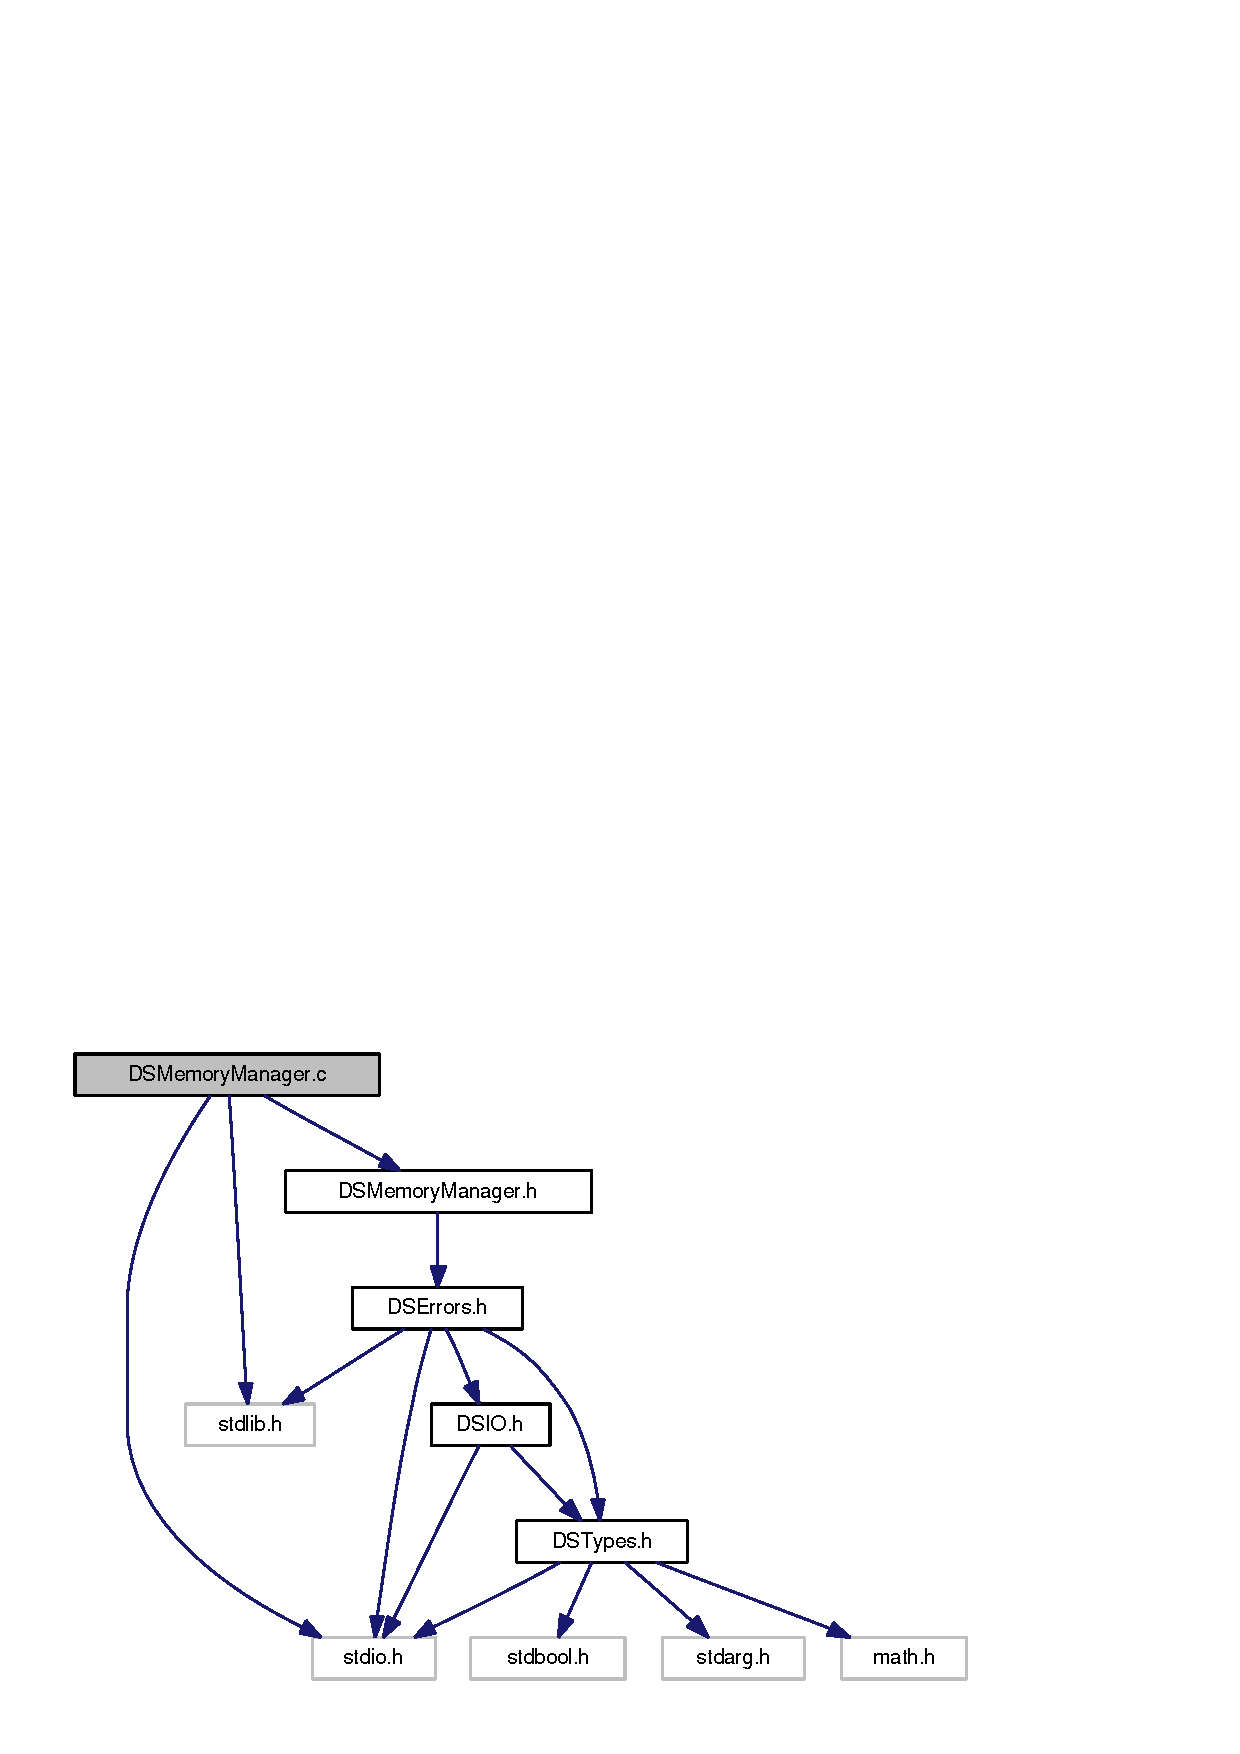
\includegraphics[width=232pt]{_d_s_memory_manager_8c__incl}
\end{center}
\end{figure}
\subsection*{Functions}
\begin{DoxyCompactItemize}
\item 
void $\ast$ \hyperlink{_d_s_memory_manager_8c_adee8e638b271ad5a066179a000e98cf2}{DSSecureMalloc} (DSInteger size)
\begin{DoxyCompactList}\small\item\em Function to securely allocate data using malloc. \item\end{DoxyCompactList}\item 
void $\ast$ \hyperlink{_d_s_memory_manager_8c_a8f23028da2b26088301ccef44cbf77da}{DSSecureCalloc} (DSInteger count, DSInteger size)
\begin{DoxyCompactList}\small\item\em Function to securely allocate data using calloc. \item\end{DoxyCompactList}\item 
void $\ast$ \hyperlink{_d_s_memory_manager_8c_a404cffa20f1d31982aa083e8ba282085}{DSSecureRealloc} (void $\ast$ptr, DSInteger size)
\begin{DoxyCompactList}\small\item\em Function to securely allocate data using realloc. \item\end{DoxyCompactList}\item 
void \hyperlink{_d_s_memory_manager_8c_abf87115fd894707c20e7efb2108d1612}{DSSecureFree} (void $\ast$ptr)
\begin{DoxyCompactList}\small\item\em Function to securely free data. \item\end{DoxyCompactList}\end{DoxyCompactItemize}


\subsection{Detailed Description}
implementation file with functions for secure memory management. This file specifies the design space standard for error handling. Contained here are the necessary macros and functions to succesfully report the errors throughout the design space library.

Copyright (C) 2011 Jason Lomnitz.\par
\par


This file is part of the Design Space Toolbox V2 (C Library).

The Design Space Toolbox V2 is free software: you can redistribute it and/or modify it under the terms of the GNU General Public License as published by the Free Software Foundation, either version 3 of the License, or (at your option) any later version.

The Design Space Toolbox V2 is distributed in the hope that it will be useful, but WITHOUT ANY WARRANTY; without even the implied warranty of MERCHANTABILITY or FITNESS FOR A PARTICULAR PURPOSE. See the GNU General Public License for more details.

You should have received a copy of the GNU General Public License along with the Design Space Toolbox. If not, see $<$\href{http://www.gnu.org/licenses/}{\tt http://www.gnu.org/licenses/}$>$.

\begin{DoxyAuthor}{Author}
Jason Lomnitz. 
\end{DoxyAuthor}
\begin{DoxyDate}{Date}
2011 
\end{DoxyDate}


\subsection{Function Documentation}
\hypertarget{_d_s_memory_manager_8c_a8f23028da2b26088301ccef44cbf77da}{
\index{DSMemoryManager.c@{DSMemoryManager.c}!DSSecureCalloc@{DSSecureCalloc}}
\index{DSSecureCalloc@{DSSecureCalloc}!DSMemoryManager.c@{DSMemoryManager.c}}
\subsubsection[{DSSecureCalloc}]{\setlength{\rightskip}{0pt plus 5cm}void$\ast$ DSSecureCalloc (DSInteger {\em count}, \/  DSInteger {\em size})}}
\label{_d_s_memory_manager_8c_a8f23028da2b26088301ccef44cbf77da}


Function to securely allocate data using calloc. 

This function is a secure calloc function which checks the allocated pointer. If the data pointer is null, indicative of errors allocating memory, the function issues a fatal error.


\begin{DoxyParams}{Parameters}
\item[{\em count}]A DSUInteger specifying the number of memory blocks being allocated. \item[{\em size}]The memory size of each block being allocated. \end{DoxyParams}
\begin{DoxyReturn}{Returns}
A pointer to the allocated data. 
\end{DoxyReturn}
\hypertarget{_d_s_memory_manager_8c_abf87115fd894707c20e7efb2108d1612}{
\index{DSMemoryManager.c@{DSMemoryManager.c}!DSSecureFree@{DSSecureFree}}
\index{DSSecureFree@{DSSecureFree}!DSMemoryManager.c@{DSMemoryManager.c}}
\subsubsection[{DSSecureFree}]{\setlength{\rightskip}{0pt plus 5cm}void DSSecureFree (void $\ast$ {\em ptr})}}
\label{_d_s_memory_manager_8c_abf87115fd894707c20e7efb2108d1612}


Function to securely free data. 

This function is a secure free function which checks the data pointer. If the data pointer is null, indicative of errors when freeing memory, the function issues a fatal error. This function calls malloc in case that pointer to be reallocated is NULL.


\begin{DoxyParams}{Parameters}
\item[{\em count}]A DSUInteger specifying the number of memory blocks being allocated. \item[{\em size}]The memory size of each block being allocated. \end{DoxyParams}
\begin{DoxyReturn}{Returns}
A pointer to the allocated data. 
\end{DoxyReturn}
\hypertarget{_d_s_memory_manager_8c_adee8e638b271ad5a066179a000e98cf2}{
\index{DSMemoryManager.c@{DSMemoryManager.c}!DSSecureMalloc@{DSSecureMalloc}}
\index{DSSecureMalloc@{DSSecureMalloc}!DSMemoryManager.c@{DSMemoryManager.c}}
\subsubsection[{DSSecureMalloc}]{\setlength{\rightskip}{0pt plus 5cm}void$\ast$ DSSecureMalloc (DSInteger {\em size})}}
\label{_d_s_memory_manager_8c_adee8e638b271ad5a066179a000e98cf2}


Function to securely allocate data using malloc. 

This function is a secure malloc function which checks the allocated pointer. If the data pointer is null, indicative of errors allocating memory, the function issues a fatal error.


\begin{DoxyParams}{Parameters}
\item[{\em size}]A DSUInteger specifying the size of memory being allocated. \end{DoxyParams}
\begin{DoxyReturn}{Returns}
A pointer to the allocated data. 
\end{DoxyReturn}
\hypertarget{_d_s_memory_manager_8c_a404cffa20f1d31982aa083e8ba282085}{
\index{DSMemoryManager.c@{DSMemoryManager.c}!DSSecureRealloc@{DSSecureRealloc}}
\index{DSSecureRealloc@{DSSecureRealloc}!DSMemoryManager.c@{DSMemoryManager.c}}
\subsubsection[{DSSecureRealloc}]{\setlength{\rightskip}{0pt plus 5cm}void$\ast$ DSSecureRealloc (void $\ast$ {\em ptr}, \/  DSInteger {\em size})}}
\label{_d_s_memory_manager_8c_a404cffa20f1d31982aa083e8ba282085}


Function to securely allocate data using realloc. 

This function is a secure realloc function which checks the allocated pointer. If the data pointer is null, indicative of errors allocating memory, the function issues a fatal error. This function calls malloc in case that pointer to be reallocated is NULL.


\begin{DoxyParams}{Parameters}
\item[{\em count}]A DSUInteger specifying the number of memory blocks being allocated. \item[{\em size}]The memory size of each block being allocated. \end{DoxyParams}
\begin{DoxyReturn}{Returns}
A pointer to the allocated data. 
\end{DoxyReturn}

\hypertarget{_d_s_memory_manager_8h}{
\section{DSMemoryManager.h File Reference}
\label{_d_s_memory_manager_8h}\index{DSMemoryManager.h@{DSMemoryManager.h}}
}


Header file with functions for secure memory allocation.  


{\ttfamily \#include \char`\"{}DSErrors.h\char`\"{}}\par
Include dependency graph for DSMemoryManager.h:\nopagebreak
\begin{figure}[H]
\begin{center}
\leavevmode
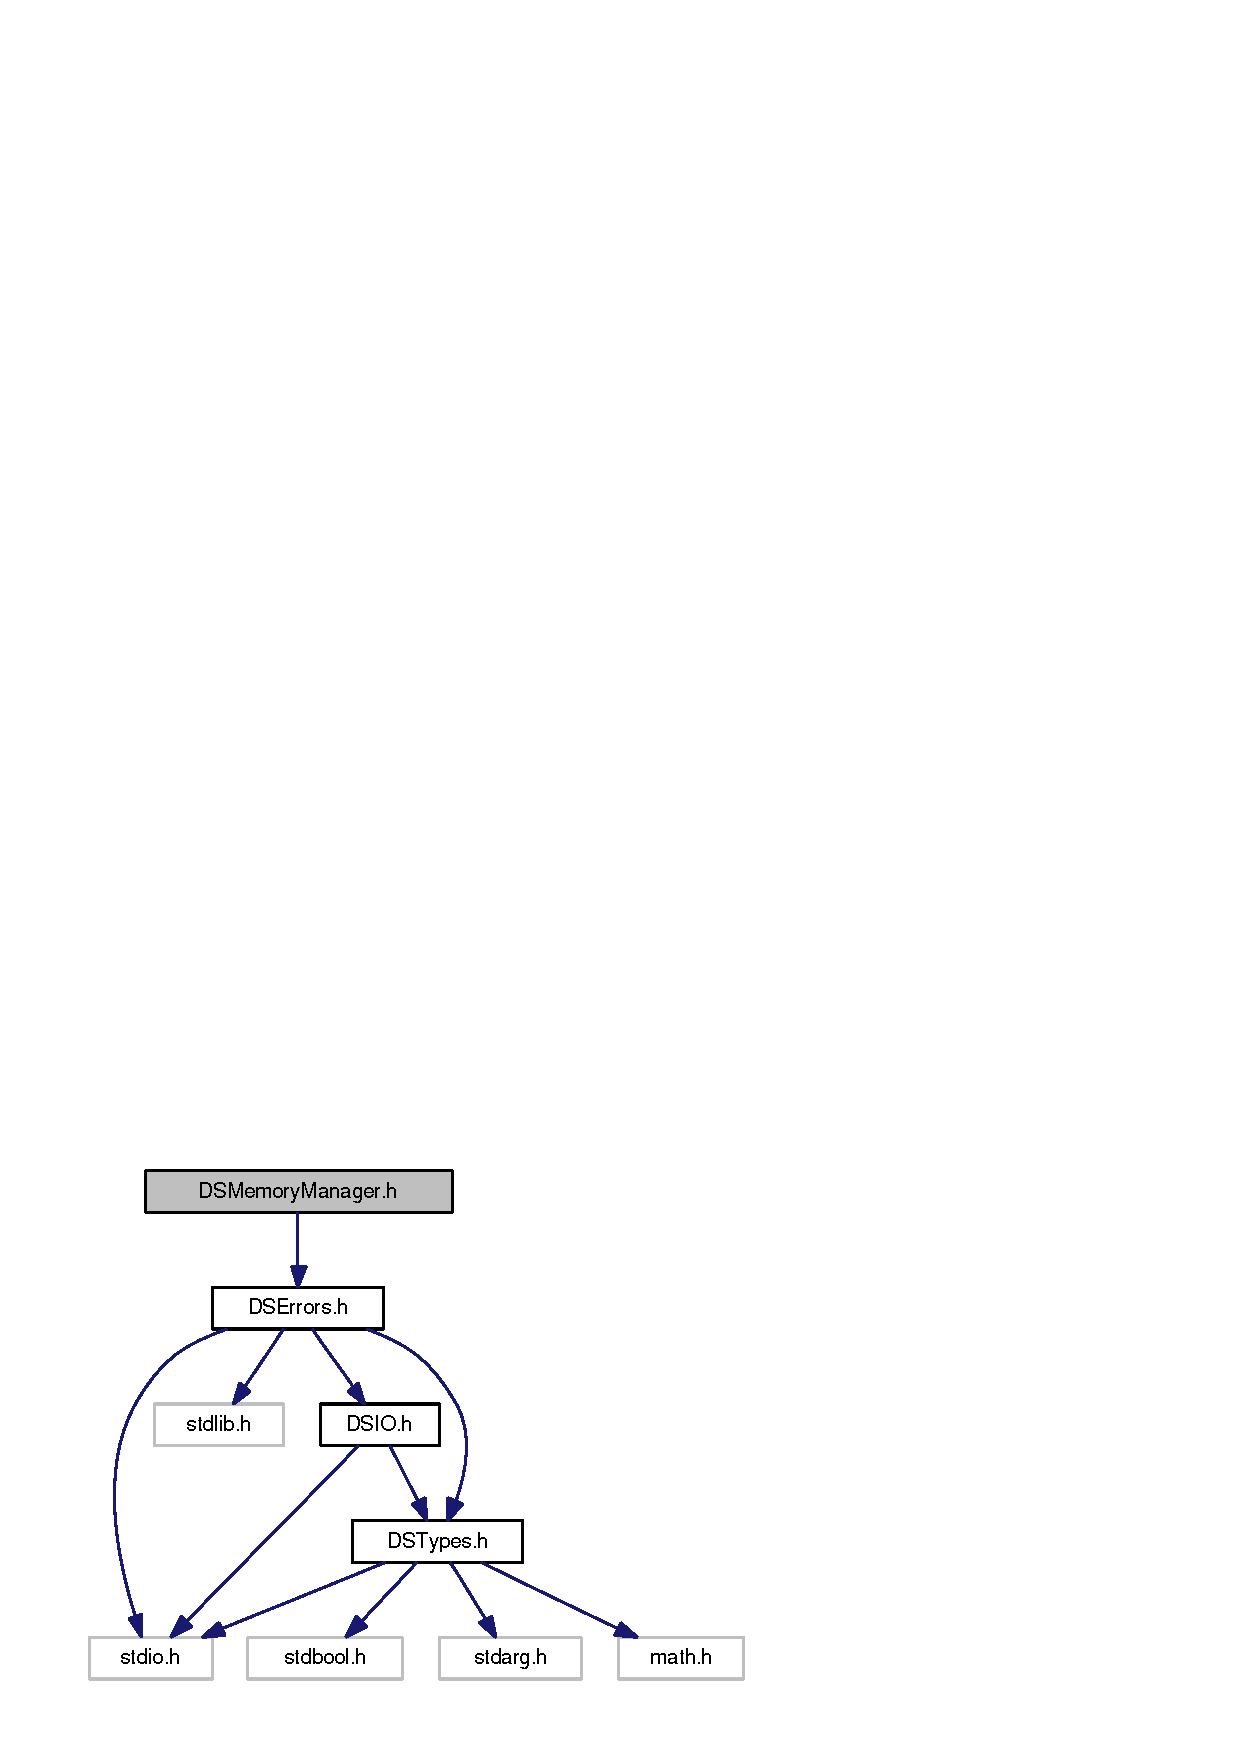
\includegraphics[width=179pt]{_d_s_memory_manager_8h__incl}
\end{center}
\end{figure}
This graph shows which files directly or indirectly include this file:\subsection*{Functions}
\begin{DoxyCompactItemize}
\item 
void $\ast$ \hyperlink{_d_s_memory_manager_8h_a9563f15fd77be4f2dbf49880f6a69bd3}{DSSecureMalloc} (size\_\-t size)
\begin{DoxyCompactList}\small\item\em Function to securely allocate data using malloc. \item\end{DoxyCompactList}\item 
void $\ast$ \hyperlink{_d_s_memory_manager_8h_a67580b5d6039a40385a68d6570b8a440}{DSSecureCalloc} (size\_\-t count, size\_\-t size)
\begin{DoxyCompactList}\small\item\em Function to securely allocate data using calloc. \item\end{DoxyCompactList}\item 
void $\ast$ \hyperlink{_d_s_memory_manager_8h_abc98af878ea31098784da0b438364757}{DSSecureRealloc} (void $\ast$ptr, size\_\-t size)
\begin{DoxyCompactList}\small\item\em Function to securely allocate data using realloc. \item\end{DoxyCompactList}\item 
void \hyperlink{_d_s_memory_manager_8h_abf87115fd894707c20e7efb2108d1612}{DSSecureFree} (void $\ast$ptr)
\begin{DoxyCompactList}\small\item\em Function to securely free data. \item\end{DoxyCompactList}\end{DoxyCompactItemize}


\subsection{Detailed Description}
Header file with functions for secure memory allocation. This file specifies the design space standard for error handling. Contained here are the necessary macros and functions to succesfully report the errors throughout the design space library.

Copyright (C) 2011 Jason Lomnitz.\par
\par


This file is part of the Design Space Toolbox V2 (C Library).

The Design Space Toolbox V2 is free software: you can redistribute it and/or modify it under the terms of the GNU General Public License as published by the Free Software Foundation, either version 3 of the License, or (at your option) any later version.

The Design Space Toolbox V2 is distributed in the hope that it will be useful, but WITHOUT ANY WARRANTY; without even the implied warranty of MERCHANTABILITY or FITNESS FOR A PARTICULAR PURPOSE. See the GNU General Public License for more details.

You should have received a copy of the GNU General Public License along with the Design Space Toolbox. If not, see $<$\href{http://www.gnu.org/licenses/}{\tt http://www.gnu.org/licenses/}$>$.

\begin{DoxyAuthor}{Author}
Jason Lomnitz. 
\end{DoxyAuthor}
\begin{DoxyDate}{Date}
2011 
\end{DoxyDate}


\subsection{Function Documentation}
\hypertarget{_d_s_memory_manager_8h_a67580b5d6039a40385a68d6570b8a440}{
\index{DSMemoryManager.h@{DSMemoryManager.h}!DSSecureCalloc@{DSSecureCalloc}}
\index{DSSecureCalloc@{DSSecureCalloc}!DSMemoryManager.h@{DSMemoryManager.h}}
\subsubsection[{DSSecureCalloc}]{\setlength{\rightskip}{0pt plus 5cm}void$\ast$ DSSecureCalloc (size\_\-t {\em count}, \/  size\_\-t {\em size})}}
\label{_d_s_memory_manager_8h_a67580b5d6039a40385a68d6570b8a440}


Function to securely allocate data using calloc. 

This function is a secure calloc function which checks the allocated pointer. If the data pointer is null, indicative of errors allocating memory, the function issues a fatal error.


\begin{DoxyParams}{Parameters}
\item[{\em count}]A DSUInteger specifying the number of memory blocks being allocated. \item[{\em size}]The memory size of each block being allocated. \end{DoxyParams}
\begin{DoxyReturn}{Returns}
A pointer to the allocated data. 
\end{DoxyReturn}
\hypertarget{_d_s_memory_manager_8h_abf87115fd894707c20e7efb2108d1612}{
\index{DSMemoryManager.h@{DSMemoryManager.h}!DSSecureFree@{DSSecureFree}}
\index{DSSecureFree@{DSSecureFree}!DSMemoryManager.h@{DSMemoryManager.h}}
\subsubsection[{DSSecureFree}]{\setlength{\rightskip}{0pt plus 5cm}void DSSecureFree (void $\ast$ {\em ptr})}}
\label{_d_s_memory_manager_8h_abf87115fd894707c20e7efb2108d1612}


Function to securely free data. 

This function is a secure free function which checks the data pointer. If the data pointer is null, indicative of errors when freeing memory, the function issues a fatal error. This function calls malloc in case that pointer to be reallocated is NULL.


\begin{DoxyParams}{Parameters}
\item[{\em count}]A DSUInteger specifying the number of memory blocks being allocated. \item[{\em size}]The memory size of each block being allocated. \end{DoxyParams}
\begin{DoxyReturn}{Returns}
A pointer to the allocated data. 
\end{DoxyReturn}
\hypertarget{_d_s_memory_manager_8h_a9563f15fd77be4f2dbf49880f6a69bd3}{
\index{DSMemoryManager.h@{DSMemoryManager.h}!DSSecureMalloc@{DSSecureMalloc}}
\index{DSSecureMalloc@{DSSecureMalloc}!DSMemoryManager.h@{DSMemoryManager.h}}
\subsubsection[{DSSecureMalloc}]{\setlength{\rightskip}{0pt plus 5cm}void$\ast$ DSSecureMalloc (size\_\-t {\em size})}}
\label{_d_s_memory_manager_8h_a9563f15fd77be4f2dbf49880f6a69bd3}


Function to securely allocate data using malloc. 

This function is a secure malloc function which checks the allocated pointer. If the data pointer is null, indicative of errors allocating memory, the function issues a fatal error.


\begin{DoxyParams}{Parameters}
\item[{\em size}]A DSUInteger specifying the size of memory being allocated. \end{DoxyParams}
\begin{DoxyReturn}{Returns}
A pointer to the allocated data. 
\end{DoxyReturn}
\hypertarget{_d_s_memory_manager_8h_abc98af878ea31098784da0b438364757}{
\index{DSMemoryManager.h@{DSMemoryManager.h}!DSSecureRealloc@{DSSecureRealloc}}
\index{DSSecureRealloc@{DSSecureRealloc}!DSMemoryManager.h@{DSMemoryManager.h}}
\subsubsection[{DSSecureRealloc}]{\setlength{\rightskip}{0pt plus 5cm}void$\ast$ DSSecureRealloc (void $\ast$ {\em ptr}, \/  size\_\-t {\em size})}}
\label{_d_s_memory_manager_8h_abc98af878ea31098784da0b438364757}


Function to securely allocate data using realloc. 

This function is a secure realloc function which checks the allocated pointer. If the data pointer is null, indicative of errors allocating memory, the function issues a fatal error. This function calls malloc in case that pointer to be reallocated is NULL.


\begin{DoxyParams}{Parameters}
\item[{\em count}]A DSUInteger specifying the number of memory blocks being allocated. \item[{\em size}]The memory size of each block being allocated. \end{DoxyParams}
\begin{DoxyReturn}{Returns}
A pointer to the allocated data. 
\end{DoxyReturn}

\hypertarget{_d_s_s_system_8h}{
\section{DSSSystem.h File Reference}
\label{_d_s_s_system_8h}\index{DSSSystem.h@{DSSSystem.h}}
}


Header file with functions for dealing with S-\/System.  


{\ttfamily \#include \char`\"{}DSTypes.h\char`\"{}}\par
Include dependency graph for DSSSystem.h:This graph shows which files directly or indirectly include this file:\subsection*{Defines}
\begin{DoxyCompactItemize}
\item 
\hypertarget{_d_s_s_system_8h_a16c8079b4cbc8f2a17538c7c53364766}{
\#define {\bfseries M\_\-DS\_\-SSYS\_\-NULL}~M\_\-DS\_\-NULL \char`\"{}: S-\/System is NULL\char`\"{}}
\label{_d_s_s_system_8h_a16c8079b4cbc8f2a17538c7c53364766}

\end{DoxyCompactItemize}
\subsection*{Functions}
\begin{DoxyCompactItemize}
\item 
\hypertarget{_d_s_s_system_8h_a918bcc35a719890cbd283c2741dc2c08}{
void {\bfseries DSSSystemFree} (\hyperlink{struct_d_s_s_system}{DSSSystem} $\ast$ssys)}
\label{_d_s_s_system_8h_a918bcc35a719890cbd283c2741dc2c08}

\item 
\hypertarget{_d_s_s_system_8h_a503c63fd680f851163a4873e2b8a270c}{
\_\-\_\-deprecated \hyperlink{struct_d_s_s_system}{DSSSystem} $\ast$ {\bfseries DSSSystemFromGMAWithDominantTerms} (const \hyperlink{struct_d_s_g_m_a_system}{DSGMASystem} $\ast$gma, const DSUInteger $\ast$termList)}
\label{_d_s_s_system_8h_a503c63fd680f851163a4873e2b8a270c}

\item 
\hypertarget{_d_s_s_system_8h_afd84cf6fdb78ce28c46e611a11310d5c}{
\hyperlink{struct_d_s_s_system}{DSSSystem} $\ast$ {\bfseries DSSSystemWithTermsFromGMA} (const \hyperlink{struct_d_s_g_m_a_system}{DSGMASystem} $\ast$gma, const DSUInteger $\ast$termArray)}
\label{_d_s_s_system_8h_afd84cf6fdb78ce28c46e611a11310d5c}

\item 
\hypertarget{_d_s_s_system_8h_a8a18055fdff2b5e1be1128f0e4f0a2f4}{
\hyperlink{struct_d_s_s_system}{DSSSystem} $\ast$ {\bfseries DSSSystemByParsingStringList} (const \hyperlink{struct_d_s_variable_pool}{DSVariablePool} $\ast$const Xd, const char $\ast$const string,...)}
\label{_d_s_s_system_8h_a8a18055fdff2b5e1be1128f0e4f0a2f4}

\item 
\hypertarget{_d_s_s_system_8h_a71291efd60229ce2b23b8a39f0a44cbf}{
\hyperlink{struct_d_s_s_system}{DSSSystem} $\ast$ {\bfseries DSSSystemByParsingStrings} (const \hyperlink{struct_d_s_variable_pool}{DSVariablePool} $\ast$const Xd, char $\ast$const $\ast$const strings, const DSUInteger numberOfEquations)}
\label{_d_s_s_system_8h_a71291efd60229ce2b23b8a39f0a44cbf}

\item 
\hypertarget{_d_s_s_system_8h_ad29393e1797e25f7e1b75548fd3cd959}{
double {\bfseries DSSSystemSteadyStateFunction} (const \hyperlink{struct_d_s_s_system}{DSSSystem} $\ast$ssys, const \hyperlink{struct_d_s_variable_pool}{DSVariablePool} $\ast$Xi0, const char $\ast$function)}
\label{_d_s_s_system_8h_ad29393e1797e25f7e1b75548fd3cd959}

\item 
\hypertarget{_d_s_s_system_8h_ac420caaa61b877f3edf89db3a9261dc0}{
\hyperlink{struct_d_s_matrix}{DSMatrix} $\ast$ {\bfseries DSSSystemSteadyStateValues} (const \hyperlink{struct_d_s_s_system}{DSSSystem} $\ast$ssys, const \hyperlink{struct_d_s_variable_pool}{DSVariablePool} $\ast$Xi0)}
\label{_d_s_s_system_8h_ac420caaa61b877f3edf89db3a9261dc0}

\item 
\hypertarget{_d_s_s_system_8h_ad0dcc109dfd59c370a9f6b8a59be94d3}{
\hyperlink{struct_d_s_matrix}{DSMatrix} $\ast$ {\bfseries DSSSystemSteadyStateFlux} (const \hyperlink{struct_d_s_s_system}{DSSSystem} $\ast$ssys, const \hyperlink{struct_d_s_variable_pool}{DSVariablePool} $\ast$Xi0)}
\label{_d_s_s_system_8h_ad0dcc109dfd59c370a9f6b8a59be94d3}

\item 
\hypertarget{_d_s_s_system_8h_a2c2c63463d29640b7750de1f96cea765}{
double {\bfseries DSSSystemLogarithmicGain} (const \hyperlink{struct_d_s_s_system}{DSSSystem} $\ast$ssys, const char $\ast$XdName, const char $\ast$XiName)}
\label{_d_s_s_system_8h_a2c2c63463d29640b7750de1f96cea765}

\item 
\hypertarget{_d_s_s_system_8h_a8ef7755c32c9997c95238670a6c52676}{
const DSUInteger {\bfseries DSSSystemNumberOfEquations} (const \hyperlink{struct_d_s_s_system}{DSSSystem} $\ast$ssys)}
\label{_d_s_s_system_8h_a8ef7755c32c9997c95238670a6c52676}

\item 
\hypertarget{_d_s_s_system_8h_a8efc2c86abcdb529b3f851b0f672804c}{
\hyperlink{structdsexpression}{DSExpression} $\ast$$\ast$ {\bfseries DSSSystemEquations} (const \hyperlink{struct_d_s_s_system}{DSSSystem} $\ast$ssys)}
\label{_d_s_s_system_8h_a8efc2c86abcdb529b3f851b0f672804c}

\item 
\hypertarget{_d_s_s_system_8h_a170d638331da941fe5b5e3025a997b15}{
\hyperlink{structdsexpression}{DSExpression} $\ast$$\ast$ {\bfseries DSSSystemSolution} (const \hyperlink{struct_d_s_s_system}{DSSSystem} $\ast$ssys)}
\label{_d_s_s_system_8h_a170d638331da941fe5b5e3025a997b15}

\item 
\hypertarget{_d_s_s_system_8h_a0cd87ab4881f4404991ecc0c87b243aa}{
\hyperlink{structdsexpression}{DSExpression} $\ast$$\ast$ {\bfseries DSSSystemLogarithmicSolution} (const \hyperlink{struct_d_s_s_system}{DSSSystem} $\ast$ssys)}
\label{_d_s_s_system_8h_a0cd87ab4881f4404991ecc0c87b243aa}

\item 
\hypertarget{_d_s_s_system_8h_a9a3b4f6a9abe3375ced44e05d875f95a}{
const \hyperlink{struct_d_s_matrix}{DSMatrix} $\ast$ {\bfseries DSSSystemAlpha} (const \hyperlink{struct_d_s_s_system}{DSSSystem} $\ast$ssys)}
\label{_d_s_s_system_8h_a9a3b4f6a9abe3375ced44e05d875f95a}

\item 
\hypertarget{_d_s_s_system_8h_a764f09f9873af8e2c8fc962a8e59d88e}{
const \hyperlink{struct_d_s_matrix}{DSMatrix} $\ast$ {\bfseries DSSSystemBeta} (const \hyperlink{struct_d_s_s_system}{DSSSystem} $\ast$ssys)}
\label{_d_s_s_system_8h_a764f09f9873af8e2c8fc962a8e59d88e}

\item 
\hypertarget{_d_s_s_system_8h_ab53ee7cbe794d8afc202d71839c58cb0}{
const \hyperlink{struct_d_s_matrix}{DSMatrix} $\ast$ {\bfseries DSSSystemGd} (const \hyperlink{struct_d_s_s_system}{DSSSystem} $\ast$ssys)}
\label{_d_s_s_system_8h_ab53ee7cbe794d8afc202d71839c58cb0}

\item 
\hypertarget{_d_s_s_system_8h_a283cec32e8288a1b252c3755224ef869}{
const \hyperlink{struct_d_s_matrix}{DSMatrix} $\ast$ {\bfseries DSSSystemGi} (const \hyperlink{struct_d_s_s_system}{DSSSystem} $\ast$ssys)}
\label{_d_s_s_system_8h_a283cec32e8288a1b252c3755224ef869}

\item 
\hypertarget{_d_s_s_system_8h_a82f0c565968c4bbd2015a15462b3a802}{
const \hyperlink{struct_d_s_matrix}{DSMatrix} $\ast$ {\bfseries DSSSystemHd} (const \hyperlink{struct_d_s_s_system}{DSSSystem} $\ast$ssys)}
\label{_d_s_s_system_8h_a82f0c565968c4bbd2015a15462b3a802}

\item 
\hypertarget{_d_s_s_system_8h_ae55c9e81f941886f385b399d8c419dee}{
const \hyperlink{struct_d_s_matrix}{DSMatrix} $\ast$ {\bfseries DSSSystemHi} (const \hyperlink{struct_d_s_s_system}{DSSSystem} $\ast$ssys)}
\label{_d_s_s_system_8h_ae55c9e81f941886f385b399d8c419dee}

\item 
\hypertarget{_d_s_s_system_8h_af8978bd4ef0e70765d827272c9191f8c}{
const \hyperlink{struct_d_s_matrix}{DSMatrix} $\ast$ {\bfseries DSSSystemM} (const \hyperlink{struct_d_s_s_system}{DSSSystem} $\ast$ssys)}
\label{_d_s_s_system_8h_af8978bd4ef0e70765d827272c9191f8c}

\item 
\hypertarget{_d_s_s_system_8h_a1d1e9352ba698c191af48268548e8a7a}{
\hyperlink{struct_d_s_matrix}{DSMatrix} $\ast$ {\bfseries DSSSystemAd} (const \hyperlink{struct_d_s_s_system}{DSSSystem} $\ast$ssys)}
\label{_d_s_s_system_8h_a1d1e9352ba698c191af48268548e8a7a}

\item 
\hypertarget{_d_s_s_system_8h_a212bdaac9db42460785d678410a9af3b}{
\hyperlink{struct_d_s_matrix}{DSMatrix} $\ast$ {\bfseries DSSSystemAi} (const \hyperlink{struct_d_s_s_system}{DSSSystem} $\ast$ssys)}
\label{_d_s_s_system_8h_a212bdaac9db42460785d678410a9af3b}

\item 
\hypertarget{_d_s_s_system_8h_a51805a26073ac81d06ea53d3fe485f8b}{
\hyperlink{struct_d_s_matrix}{DSMatrix} $\ast$ {\bfseries DSSSystemB} (const \hyperlink{struct_d_s_s_system}{DSSSystem} $\ast$ssys)}
\label{_d_s_s_system_8h_a51805a26073ac81d06ea53d3fe485f8b}

\item 
\hypertarget{_d_s_s_system_8h_a4b015039900d5c07f180127e310cdca4}{
\hyperlink{struct_d_s_matrix}{DSMatrix} $\ast$ {\bfseries DSSSystemA} (const \hyperlink{struct_d_s_s_system}{DSSSystem} $\ast$ssys)}
\label{_d_s_s_system_8h_a4b015039900d5c07f180127e310cdca4}

\item 
\hypertarget{_d_s_s_system_8h_a773b984ac5761bec7af37cafdbf7706f}{
\hyperlink{struct_d_s_matrix}{DSMatrix} $\ast$ {\bfseries DSSSystemG} (const \hyperlink{struct_d_s_s_system}{DSSSystem} $\ast$ssys)}
\label{_d_s_s_system_8h_a773b984ac5761bec7af37cafdbf7706f}

\item 
\hypertarget{_d_s_s_system_8h_a5a49260995d086491bbfafd399235530}{
\hyperlink{struct_d_s_matrix}{DSMatrix} $\ast$ {\bfseries DSSSystemH} (const \hyperlink{struct_d_s_s_system}{DSSSystem} $\ast$ssys)}
\label{_d_s_s_system_8h_a5a49260995d086491bbfafd399235530}

\item 
\hypertarget{_d_s_s_system_8h_ae0feec4d3c4e10f39d0bdb74f65c244d}{
const \hyperlink{struct_d_s_variable_pool}{DSVariablePool} $\ast$ {\bfseries DSSSystemXd} (const \hyperlink{struct_d_s_s_system}{DSSSystem} $\ast$const ssys)}
\label{_d_s_s_system_8h_ae0feec4d3c4e10f39d0bdb74f65c244d}

\item 
\hypertarget{_d_s_s_system_8h_a43309ae0043c77df7f70d54d9b70a1c5}{
const \hyperlink{struct_d_s_variable_pool}{DSVariablePool} $\ast$ {\bfseries DSSSystemXi} (const \hyperlink{struct_d_s_s_system}{DSSSystem} $\ast$const ssys)}
\label{_d_s_s_system_8h_a43309ae0043c77df7f70d54d9b70a1c5}

\item 
\hypertarget{_d_s_s_system_8h_abc405834b14a3a34cb45c40be6f61939}{
const bool {\bfseries DSSSystemHasSolution} (const \hyperlink{struct_d_s_s_system}{DSSSystem} $\ast$ssys)}
\label{_d_s_s_system_8h_abc405834b14a3a34cb45c40be6f61939}

\item 
\hypertarget{_d_s_s_system_8h_a39b9fec2a3f14b0dd499093af9bd0ac3}{
const bool {\bfseries DSSSystemIsSingular} (const \hyperlink{struct_d_s_s_system}{DSSSystem} $\ast$ssys)}
\label{_d_s_s_system_8h_a39b9fec2a3f14b0dd499093af9bd0ac3}

\item 
\hypertarget{_d_s_s_system_8h_aa49a5035055d1520458f0dbec259302d}{
void {\bfseries DSSSystemPrint} (const \hyperlink{struct_d_s_s_system}{DSSSystem} $\ast$ssys)}
\label{_d_s_s_system_8h_aa49a5035055d1520458f0dbec259302d}

\item 
\hypertarget{_d_s_s_system_8h_a7d99eec40ba2f76950196564259aae6d}{
void {\bfseries DSSSystemPrintEquations} (const \hyperlink{struct_d_s_s_system}{DSSSystem} $\ast$ssys)}
\label{_d_s_s_system_8h_a7d99eec40ba2f76950196564259aae6d}

\item 
\hypertarget{_d_s_s_system_8h_a4ef67a113a97c2a91796f0c3065fe0aa}{
void {\bfseries DSSSystemPrintSolution} (const \hyperlink{struct_d_s_s_system}{DSSSystem} $\ast$ssys)}
\label{_d_s_s_system_8h_a4ef67a113a97c2a91796f0c3065fe0aa}

\item 
\hypertarget{_d_s_s_system_8h_a7db3262e6d2b87e643a7930f6ad7bfb9}{
void {\bfseries DSSSystemPrintLogarithmicSolution} (const \hyperlink{struct_d_s_s_system}{DSSSystem} $\ast$ssys)}
\label{_d_s_s_system_8h_a7db3262e6d2b87e643a7930f6ad7bfb9}

\end{DoxyCompactItemize}


\subsection{Detailed Description}
Header file with functions for dealing with S-\/System. Copyright (C) 2011 Jason Lomnitz.\par
\par


This file is part of the Design Space Toolbox V2 (C Library).

The Design Space Toolbox V2 is free software: you can redistribute it and/or modify it under the terms of the GNU General Public License as published by the Free Software Foundation, either version 3 of the License, or (at your option) any later version.

The Design Space Toolbox V2 is distributed in the hope that it will be useful, but WITHOUT ANY WARRANTY; without even the implied warranty of MERCHANTABILITY or FITNESS FOR A PARTICULAR PURPOSE. See the GNU General Public License for more details.

You should have received a copy of the GNU General Public License along with the Design Space Toolbox. If not, see $<$\href{http://www.gnu.org/licenses/}{\tt http://www.gnu.org/licenses/}$>$.

\begin{DoxyAuthor}{Author}
Jason Lomnitz. 
\end{DoxyAuthor}
\begin{DoxyDate}{Date}
2011 
\end{DoxyDate}

\hypertarget{_d_s_std_8h}{
\section{DSStd.h File Reference}
\label{_d_s_std_8h}\index{DSStd.h@{DSStd.h}}
}


Header file for the design space toolbox.  


{\ttfamily \#include $<$stdio.h$>$}\par
{\ttfamily \#include $<$stdlib.h$>$}\par
{\ttfamily \#include \char`\"{}DSTypes.h\char`\"{}}\par
{\ttfamily \#include \char`\"{}DSIO.h\char`\"{}}\par
{\ttfamily \#include \char`\"{}DSErrors.h\char`\"{}}\par
{\ttfamily \#include \char`\"{}DSMemoryManager.h\char`\"{}}\par
{\ttfamily \#include \char`\"{}DSVariable.h\char`\"{}}\par
{\ttfamily \#include \char`\"{}DSMatrix.h\char`\"{}}\par
{\ttfamily \#include \char`\"{}DSMatrixArray.h\char`\"{}}\par
Include dependency graph for DSStd.h:\nopagebreak
\begin{figure}[H]
\begin{center}
\leavevmode
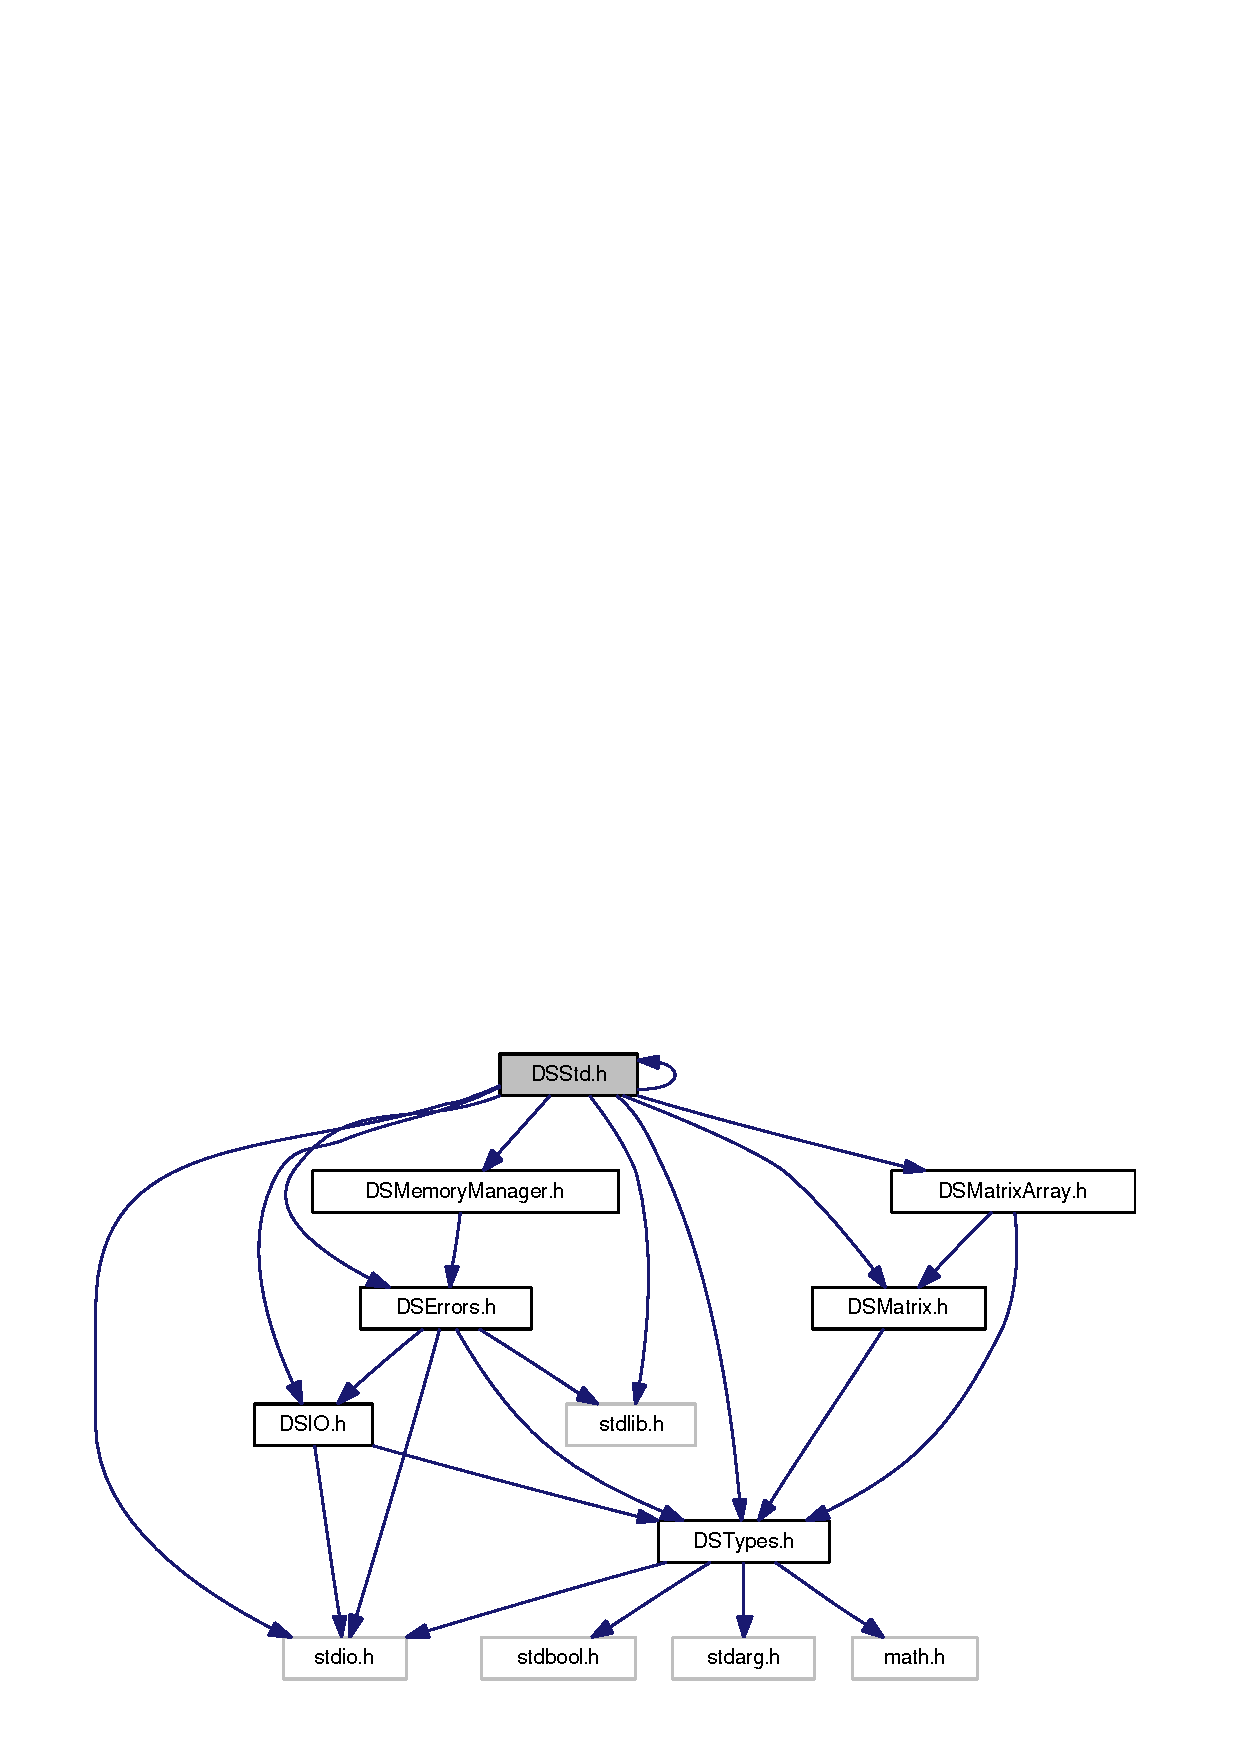
\includegraphics[width=272pt]{_d_s_std_8h__incl}
\end{center}
\end{figure}
This graph shows which files directly or indirectly include this file:\nopagebreak
\begin{figure}[H]
\begin{center}
\leavevmode
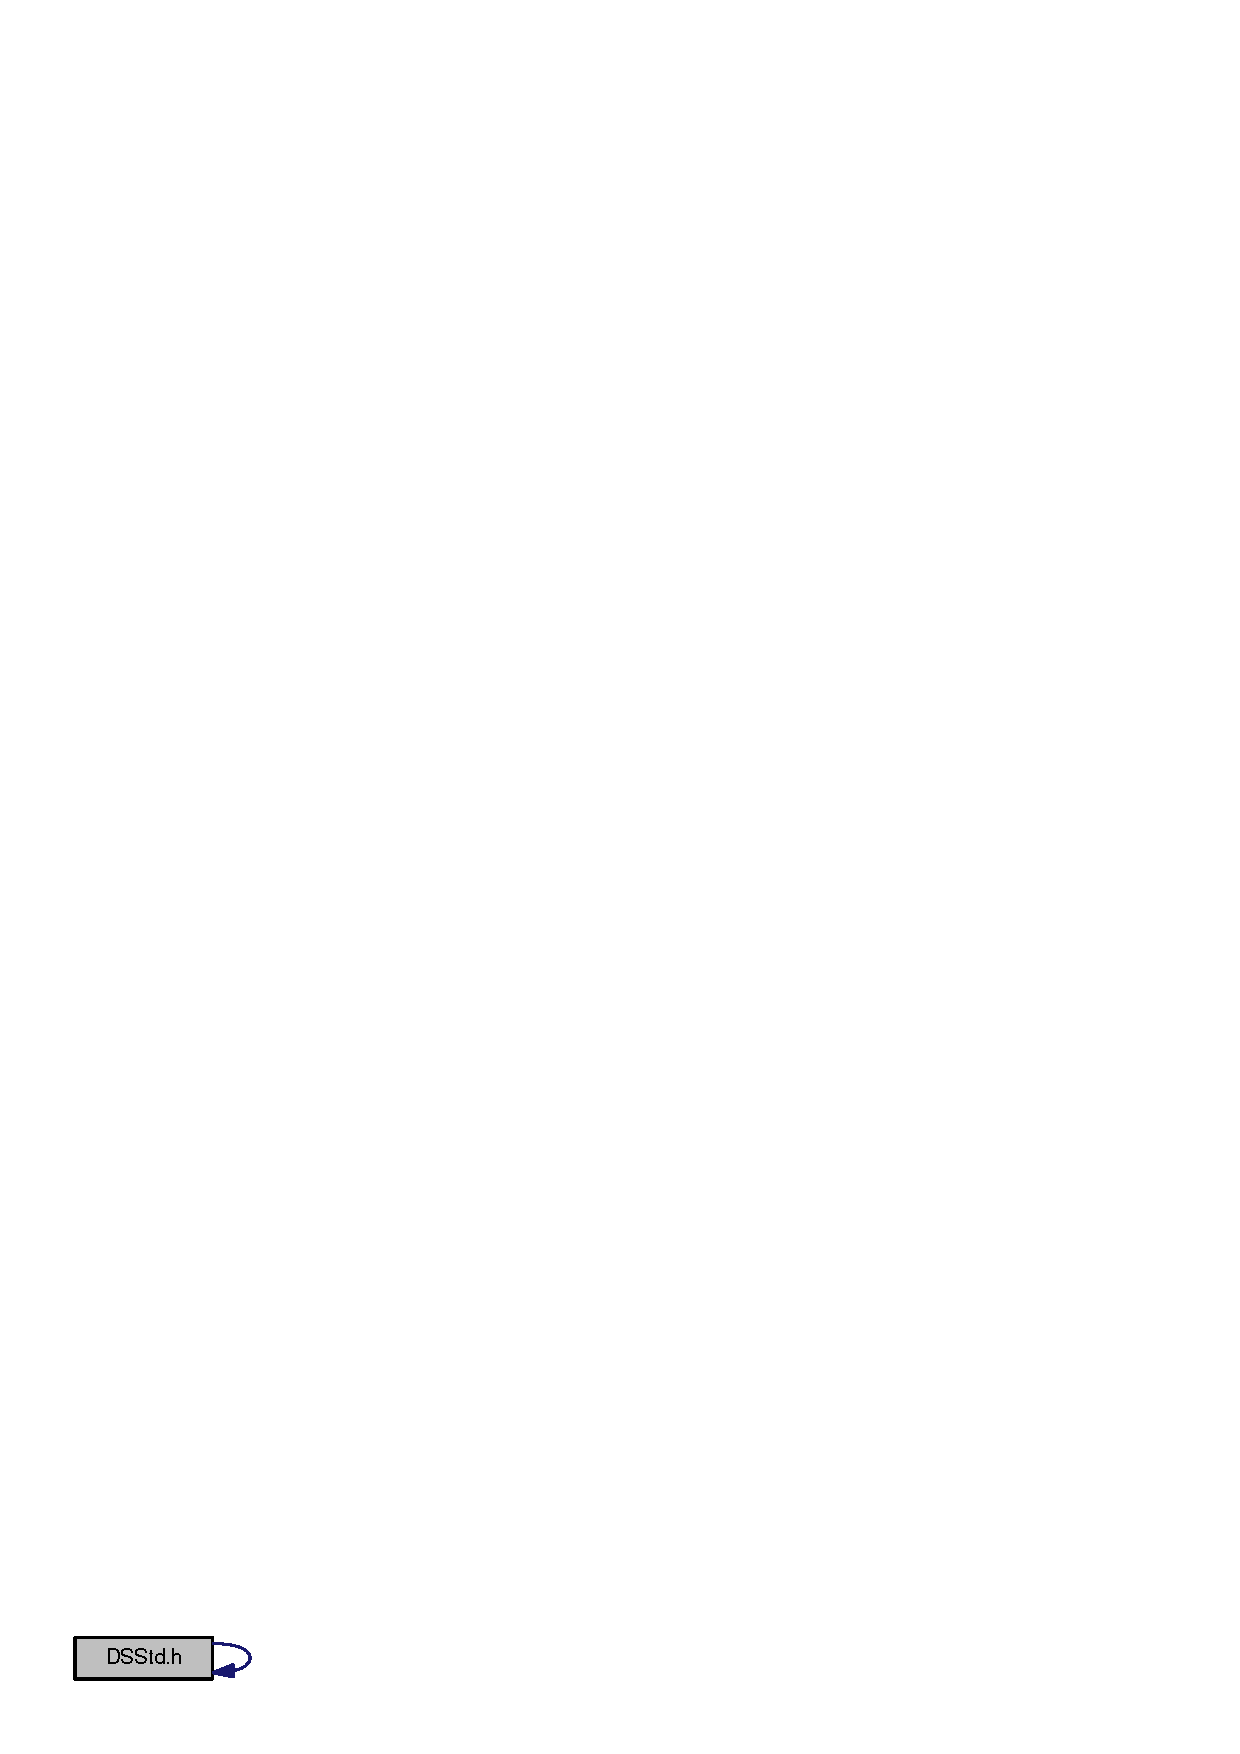
\includegraphics[width=60pt]{_d_s_std_8h__dep__incl}
\end{center}
\end{figure}


\subsection{Detailed Description}
Header file for the design space toolbox. Copyright (C) 2011 Jason Lomnitz.\par
\par


This file is part of the Design Space Toolbox V2 (C Library).

The Design Space Toolbox V2 is free software: you can redistribute it and/or modify it under the terms of the GNU General Public License as published by the Free Software Foundation, either version 3 of the License, or (at your option) any later version.

The Design Space Toolbox V2 is distributed in the hope that it will be useful, but WITHOUT ANY WARRANTY; without even the implied warranty of MERCHANTABILITY or FITNESS FOR A PARTICULAR PURPOSE. See the GNU General Public License for more details.

You should have received a copy of the GNU General Public License along with the Design Space Toolbox. If not, see $<$\href{http://www.gnu.org/licenses/}{\tt http://www.gnu.org/licenses/}$>$.

\begin{DoxyAuthor}{Author}
Jason Lomnitz. 
\end{DoxyAuthor}
\begin{DoxyDate}{Date}
2011
\end{DoxyDate}
\begin{Desc}
\item[\hyperlink{todo__todo000002}{Todo}]Add all previous functionality. 

Add vertex enumeration functionality.\end{Desc}

\hypertarget{_d_s_symbolic_matrix_8h}{
\section{DSSymbolicMatrix.h File Reference}
\label{_d_s_symbolic_matrix_8h}\index{DSSymbolicMatrix.h@{DSSymbolicMatrix.h}}
}


Header file with functions for dealing with symbolic matrices.  


{\ttfamily \#include \char`\"{}DSTypes.h\char`\"{}}\par
{\ttfamily \#include \char`\"{}DSErrors.h\char`\"{}}\par
{\ttfamily \#include \char`\"{}DSIO.h\char`\"{}}\par
Include dependency graph for DSSymbolicMatrix.h:\subsection*{Defines}
\begin{DoxyCompactItemize}
\item 
\hypertarget{group___m___d_s___messages_gab1c842ea678de8daa76a55fc68750d5e}{
\#define \hyperlink{group___m___d_s___messages_gab1c842ea678de8daa76a55fc68750d5e}{M\_\-DS\_\-SYM\_\-MAT\_\-NULL}~\char`\"{}Pointer to symbolic matrix is NULL\char`\"{}}
\label{group___m___d_s___messages_gab1c842ea678de8daa76a55fc68750d5e}

\begin{DoxyCompactList}\small\item\em Message for a NULL \hyperlink{struct_d_s_matrix}{DSMatrix} pointer. \item\end{DoxyCompactList}\item 
\hypertarget{group___m___d_s___messages_gad8ee7418e1f3268fa9841bc7d7fcf898}{
\#define \hyperlink{group___m___d_s___messages_gad8ee7418e1f3268fa9841bc7d7fcf898}{M\_\-DS\_\-SYM\_\-MAT\_\-OUTOFBOUNDS}~\char`\"{}Row or column out of bounds\char`\"{}}
\label{group___m___d_s___messages_gad8ee7418e1f3268fa9841bc7d7fcf898}

\begin{DoxyCompactList}\small\item\em Message for a row or column exceeding matrix bounds. \item\end{DoxyCompactList}\item 
\hypertarget{group___m___d_s___messages_ga24ff99c3a2bfe77b32048fa05cb19a44}{
\#define \hyperlink{group___m___d_s___messages_ga24ff99c3a2bfe77b32048fa05cb19a44}{M\_\-DS\_\-SYM\_\-MAT\_\-NOINTERNAL}~\char`\"{}Matrix data is empty\char`\"{}}
\label{group___m___d_s___messages_ga24ff99c3a2bfe77b32048fa05cb19a44}

\begin{DoxyCompactList}\small\item\em Message for a NULL internal matrix structure. \item\end{DoxyCompactList}\end{DoxyCompactItemize}
\subsection*{Functions}
\begin{DoxyCompactItemize}
\item 
\hypertarget{_d_s_symbolic_matrix_8h_a4b7fd098bd8dc965978aa00d57c2c7d5}{
\hyperlink{struct_d_s_symbolic_matrix}{DSSymbolicMatrix} $\ast$ {\bfseries DSSymbolicMatrixAlloc} (const DSUInteger rows, const DSUInteger columns)}
\label{_d_s_symbolic_matrix_8h_a4b7fd098bd8dc965978aa00d57c2c7d5}

\item 
\hypertarget{_d_s_symbolic_matrix_8h_a492cf3083fe5c0eaadabe88bf08f7de3}{
\hyperlink{struct_d_s_symbolic_matrix}{DSSymbolicMatrix} $\ast$ {\bfseries DSSymbolicMatrixCalloc} (const DSUInteger rows, const DSUInteger columns)}
\label{_d_s_symbolic_matrix_8h_a492cf3083fe5c0eaadabe88bf08f7de3}

\item 
\hypertarget{_d_s_symbolic_matrix_8h_a0188961f55294e306fcc0a79a6151663}{
\hyperlink{struct_d_s_symbolic_matrix}{DSSymbolicMatrix} $\ast$ {\bfseries DSSymbolicMatrixCopy} (const \hyperlink{struct_d_s_symbolic_matrix}{DSSymbolicMatrix} $\ast$original)}
\label{_d_s_symbolic_matrix_8h_a0188961f55294e306fcc0a79a6151663}

\item 
\hypertarget{_d_s_symbolic_matrix_8h_a4055044640592f91b929344c06ddcf8b}{
void {\bfseries DSSymbolicMatrixFree} (\hyperlink{struct_d_s_symbolic_matrix}{DSSymbolicMatrix} $\ast$matrix)}
\label{_d_s_symbolic_matrix_8h_a4055044640592f91b929344c06ddcf8b}

\item 
\hypertarget{_d_s_symbolic_matrix_8h_af21334df2f4a1bf2edc0791f7e1bff6c}{
\hyperlink{struct_d_s_symbolic_matrix}{DSSymbolicMatrix} $\ast$ {\bfseries DSSymbolicMatrixIdentity} (const DSUInteger size)}
\label{_d_s_symbolic_matrix_8h_af21334df2f4a1bf2edc0791f7e1bff6c}

\item 
\hypertarget{_d_s_symbolic_matrix_8h_a0c6936024d354fec921095f9547b86a6}{
\hyperlink{struct_d_s_symbolic_matrix}{DSSymbolicMatrix} $\ast$ {\bfseries DSSymbolicMatrixRandomNumbers} (const DSUInteger rows, const DSUInteger columns)}
\label{_d_s_symbolic_matrix_8h_a0c6936024d354fec921095f9547b86a6}

\item 
\hypertarget{_d_s_symbolic_matrix_8h_a8f195b67eea1c1f4d6c58670f2a5846b}{
\hyperlink{struct_d_s_symbolic_matrix}{DSSymbolicMatrix} $\ast$ {\bfseries DSSymbolicMatrixByParsingString} (const char $\ast$string)}
\label{_d_s_symbolic_matrix_8h_a8f195b67eea1c1f4d6c58670f2a5846b}

\item 
\hypertarget{_d_s_symbolic_matrix_8h_a4ec0ac21882b231201349f02f9f548ba}{
double {\bfseries DSSymbolicMatrixDoubleByEvaluatingExpression} (const \hyperlink{struct_d_s_symbolic_matrix}{DSSymbolicMatrix} $\ast$matrix, const DSUInteger row, const DSUInteger column, const \hyperlink{struct_d_s_variable_pool}{DSVariablePool} $\ast$variableValues)}
\label{_d_s_symbolic_matrix_8h_a4ec0ac21882b231201349f02f9f548ba}

\item 
\hypertarget{_d_s_symbolic_matrix_8h_a6e1d4efa6febaa15824b83d13d589ba6}{
const \hyperlink{structdsexpression}{DSExpression} $\ast$ {\bfseries DSSymbolicMatrixExpression} (const \hyperlink{struct_d_s_symbolic_matrix}{DSSymbolicMatrix} $\ast$matrix, const DSUInteger row, const DSUInteger column)}
\label{_d_s_symbolic_matrix_8h_a6e1d4efa6febaa15824b83d13d589ba6}

\item 
\hypertarget{_d_s_symbolic_matrix_8h_a7b70b30e6b36de2fb046499a68f8040e}{
void {\bfseries DSSymbolicMatrixSetExpression} (\hyperlink{struct_d_s_symbolic_matrix}{DSSymbolicMatrix} $\ast$matrix, const DSUInteger row, const DSUInteger column, const \hyperlink{structdsexpression}{DSExpression} $\ast$expr)}
\label{_d_s_symbolic_matrix_8h_a7b70b30e6b36de2fb046499a68f8040e}

\item 
\hypertarget{_d_s_symbolic_matrix_8h_a3f5d9df863ea543a3eaa7fa730356798}{
DSUInteger {\bfseries DSSymbolicMatrixRows} (const \hyperlink{struct_d_s_symbolic_matrix}{DSSymbolicMatrix} $\ast$matrix)}
\label{_d_s_symbolic_matrix_8h_a3f5d9df863ea543a3eaa7fa730356798}

\item 
\hypertarget{_d_s_symbolic_matrix_8h_afe15ec211669bc9320c621aead760ba5}{
DSUInteger {\bfseries DSSymbolicMatrixColumns} (const \hyperlink{struct_d_s_symbolic_matrix}{DSSymbolicMatrix} $\ast$matrix)}
\label{_d_s_symbolic_matrix_8h_afe15ec211669bc9320c621aead760ba5}

\item 
\hypertarget{_d_s_symbolic_matrix_8h_abe0e3c607cd22a51368300c14f5cca1c}{
\hyperlink{struct_d_s_matrix}{DSMatrix} $\ast$ {\bfseries DSSymbolicMatrixToNumericalMatrix} (const \hyperlink{struct_d_s_symbolic_matrix}{DSSymbolicMatrix} $\ast$matrix, const \hyperlink{struct_d_s_variable_pool}{DSVariablePool} $\ast$variables)}
\label{_d_s_symbolic_matrix_8h_abe0e3c607cd22a51368300c14f5cca1c}

\end{DoxyCompactItemize}


\subsection{Detailed Description}
Header file with functions for dealing with symbolic matrices. Copyright (C) 2011 Jason Lomnitz.\par
\par


This file is part of the Design Space Toolbox V2 (C Library).

The Design Space Toolbox V2 is free software: you can redistribute it and/or modify it under the terms of the GNU General Public License as published by the Free Software Foundation, either version 3 of the License, or (at your option) any later version.

The Design Space Toolbox V2 is distributed in the hope that it will be useful, but WITHOUT ANY WARRANTY; without even the implied warranty of MERCHANTABILITY or FITNESS FOR A PARTICULAR PURPOSE. See the GNU General Public License for more details.

You should have received a copy of the GNU General Public License along with the Design Space Toolbox. If not, see $<$\href{http://www.gnu.org/licenses/}{\tt http://www.gnu.org/licenses/}$>$.

\begin{DoxyAuthor}{Author}
Jason Lomnitz. 
\end{DoxyAuthor}
\begin{DoxyDate}{Date}
2011 
\end{DoxyDate}

\hypertarget{_d_s_types_8h}{
\section{DSTypes.h File Reference}
\label{_d_s_types_8h}\index{DSTypes.h@{DSTypes.h}}
}


Header file with definitions for data types.  


{\ttfamily \#include $<$stdio.h$>$}\par
{\ttfamily \#include $<$stdbool.h$>$}\par
{\ttfamily \#include $<$stdarg.h$>$}\par
{\ttfamily \#include $<$math.h$>$}\par
Include dependency graph for DSTypes.h:\nopagebreak
\begin{figure}[H]
\begin{center}
\leavevmode
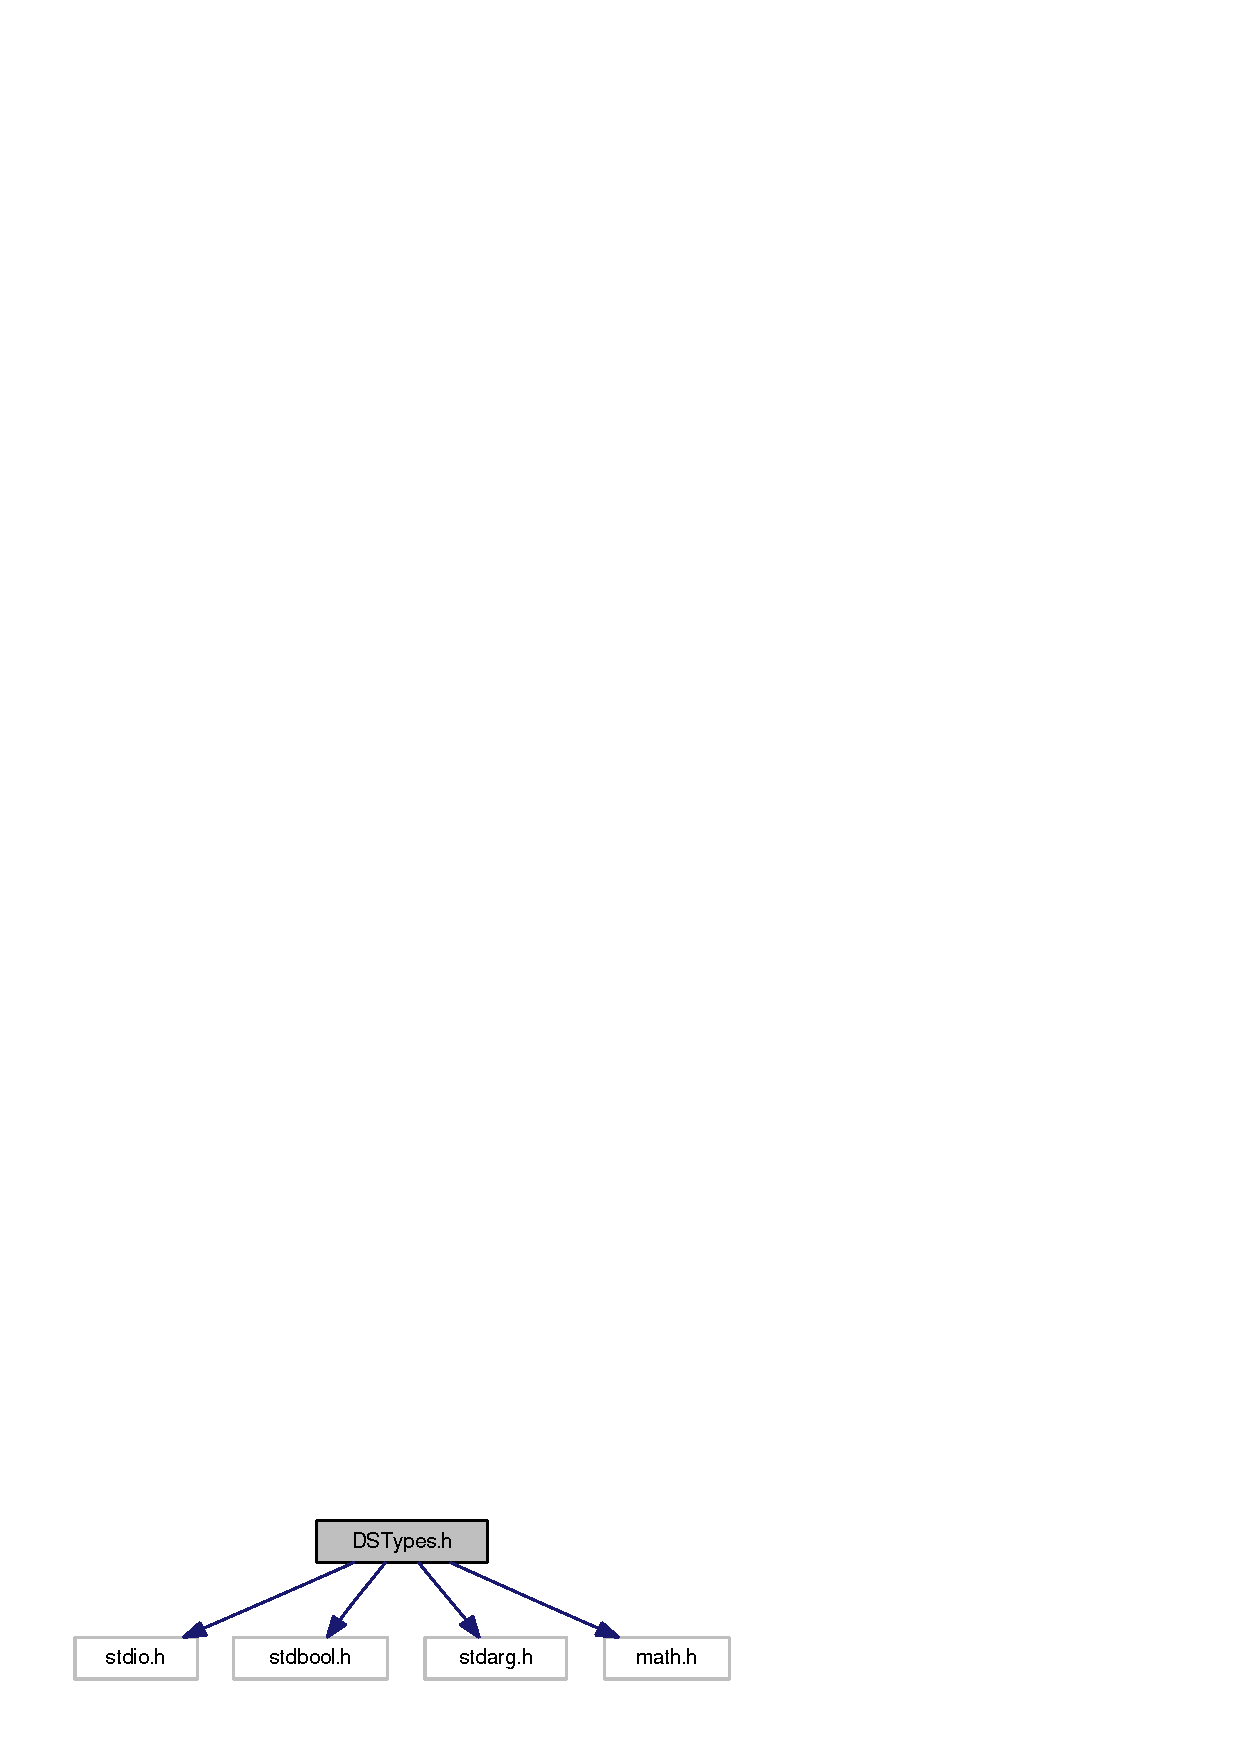
\includegraphics[width=175pt]{_d_s_types_8h__incl}
\end{center}
\end{figure}
This graph shows which files directly or indirectly include this file:\nopagebreak
\begin{figure}[H]
\begin{center}
\leavevmode
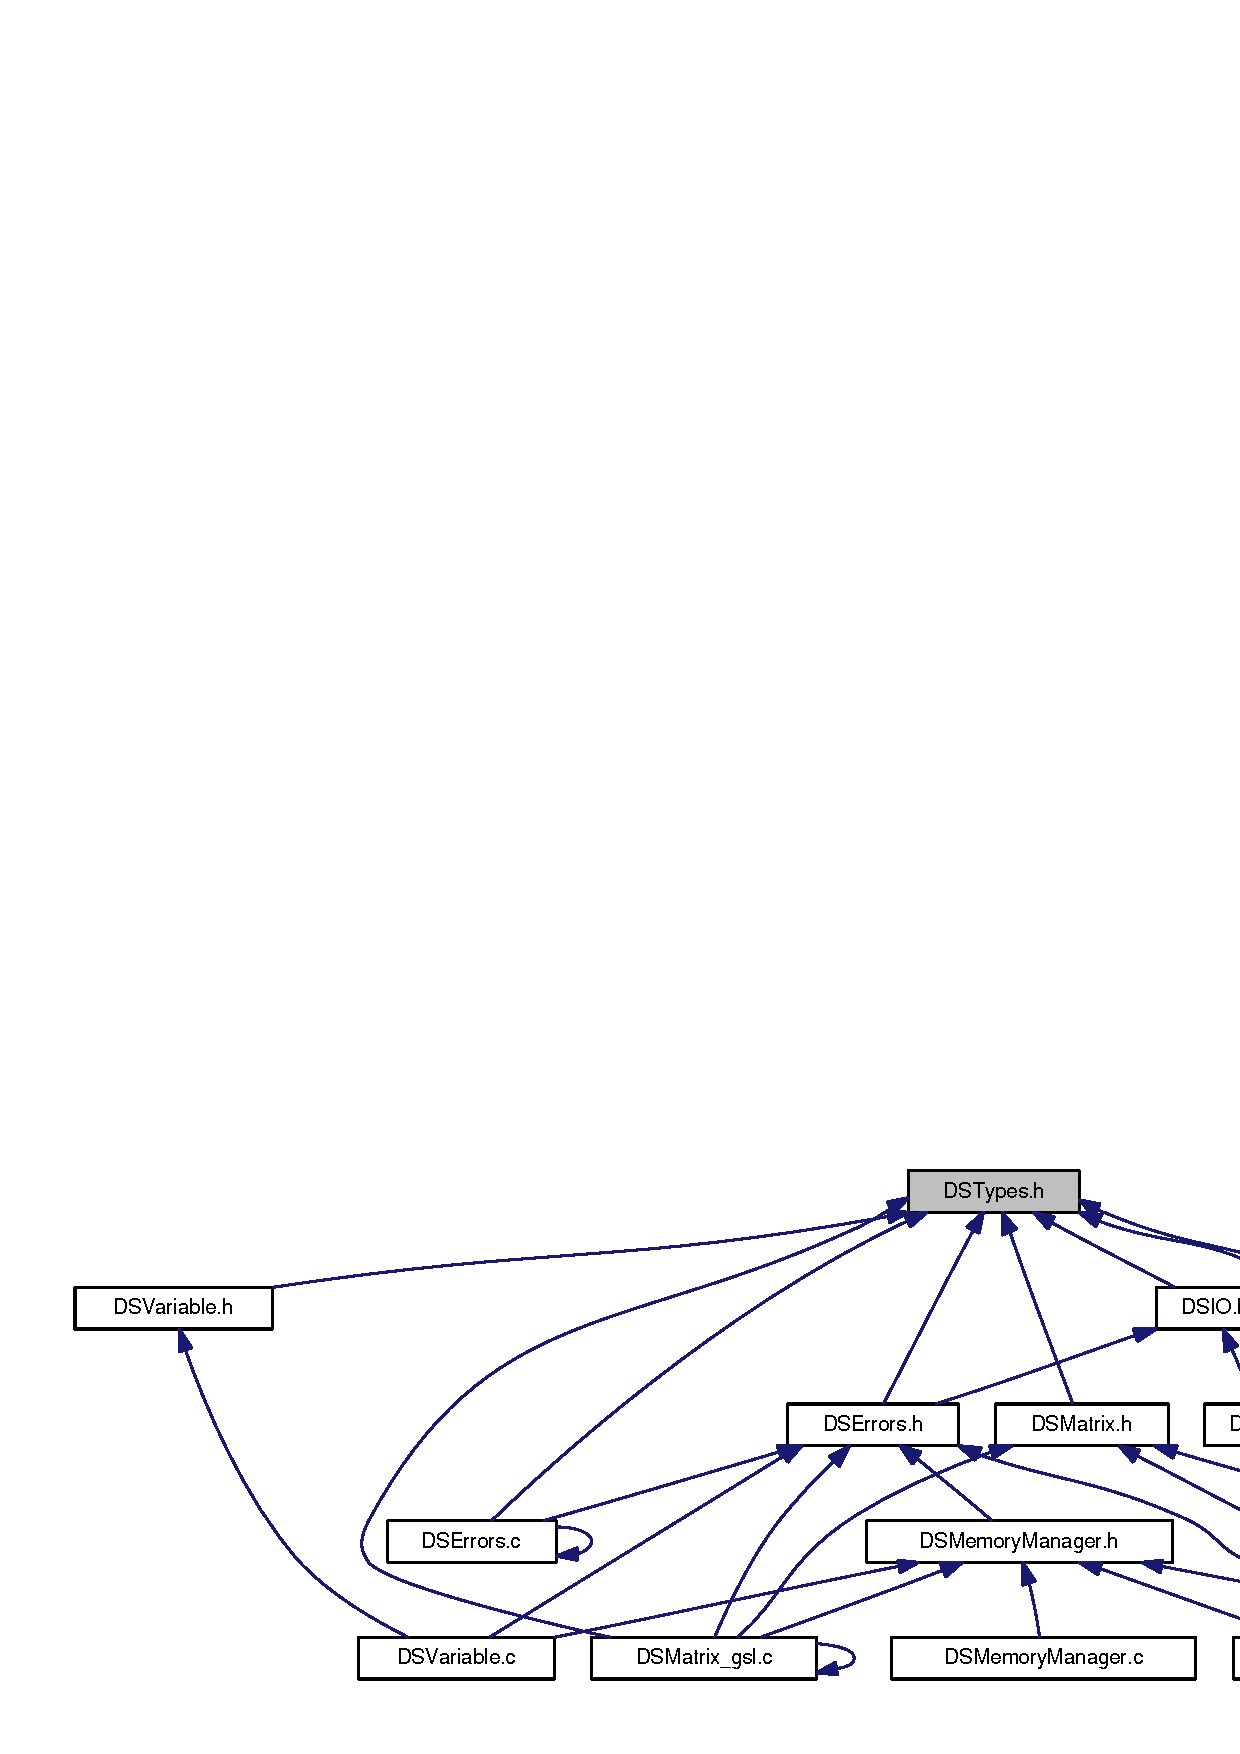
\includegraphics[width=420pt]{_d_s_types_8h__dep__incl}
\end{center}
\end{figure}
\subsection*{Data Structures}
\begin{DoxyCompactItemize}
\item 
struct \hyperlink{struct_d_s_variable}{DSVariable}
\begin{DoxyCompactList}\small\item\em Data type that is used to store errors. \item\end{DoxyCompactList}\item 
struct \hyperlink{struct__var_dictionary}{\_\-varDictionary}
\begin{DoxyCompactList}\small\item\em Internal dictionary structure. \item\end{DoxyCompactList}\item 
struct \hyperlink{struct_d_s_matrix}{DSMatrix}
\begin{DoxyCompactList}\small\item\em Data type representing a matrix. \item\end{DoxyCompactList}\item 
struct \hyperlink{struct_d_s_matrix_array}{DSMatrixArray}
\begin{DoxyCompactList}\small\item\em Data type representing an array of matrices. \item\end{DoxyCompactList}\item 
struct \hyperlink{struct_d_s_s_system}{DSSSystem}
\begin{DoxyCompactList}\small\item\em Data type representing an S-\/System. \item\end{DoxyCompactList}\end{DoxyCompactItemize}
\subsection*{Defines}
\begin{DoxyCompactItemize}
\item 
\hypertarget{_d_s_types_8h_aa0c1167bb311135eecf24a0e7c885b7f}{
\#define {\bfseries endif}}
\label{_d_s_types_8h_aa0c1167bb311135eecf24a0e7c885b7f}

\item 
\hypertarget{_d_s_types_8h_a4e1585cb1b8a465a6a9a702d97bb4ad8}{
\#define {\bfseries \_\-\_\-deprecated}}
\label{_d_s_types_8h_a4e1585cb1b8a465a6a9a702d97bb4ad8}

\item 
\hypertarget{_d_s_types_8h_a956e2723d559858d08644ac99146e910}{
\#define {\bfseries INFINITY}~HUGE\_\-VAL}
\label{_d_s_types_8h_a956e2723d559858d08644ac99146e910}

\end{DoxyCompactItemize}
\subsection*{Typedefs}
\begin{DoxyCompactItemize}
\item 
\hypertarget{_d_s_types_8h_acd52f160f8edb3f2c7c4ba8d9ddcd025}{
typedef int {\bfseries DSInteger}}
\label{_d_s_types_8h_acd52f160f8edb3f2c7c4ba8d9ddcd025}

\item 
\hypertarget{_d_s_types_8h_a176fc92c26d2116f67d6043e728adbb5}{
typedef unsigned int {\bfseries DSUInteger}}
\label{_d_s_types_8h_a176fc92c26d2116f67d6043e728adbb5}

\item 
typedef struct \hyperlink{struct__var_dictionary}{\_\-varDictionary} \hyperlink{_d_s_types_8h_a67b340fa4a564cc84d27b3647ef1ad75}{DSVariablePool}
\begin{DoxyCompactList}\small\item\em Internal dictionary structure. \item\end{DoxyCompactList}\end{DoxyCompactItemize}


\subsection{Detailed Description}
Header file with definitions for data types. This file specifies the design space standard data types. Contained here are strictly the data type definitions, and specific macros to access data in data structures. Functions applying to these data types are contained elsewhere, and the individual data structures should refer to these files.

Copyright (C) 2011 Jason Lomnitz.\par
\par


This file is part of the Design Space Toolbox V2 (C Library).

The Design Space Toolbox V2 is free software: you can redistribute it and/or modify it under the terms of the GNU General Public License as published by the Free Software Foundation, either version 3 of the License, or (at your option) any later version.

The Design Space Toolbox V2 is distributed in the hope that it will be useful, but WITHOUT ANY WARRANTY; without even the implied warranty of MERCHANTABILITY or FITNESS FOR A PARTICULAR PURPOSE. See the GNU General Public License for more details.

You should have received a copy of the GNU General Public License along with the Design Space Toolbox. If not, see $<$\href{http://www.gnu.org/licenses/}{\tt http://www.gnu.org/licenses/}$>$.

\begin{DoxyAuthor}{Author}
Jason Lomnitz. 
\end{DoxyAuthor}
\begin{DoxyDate}{Date}
2011 
\end{DoxyDate}


\subsection{Typedef Documentation}
\hypertarget{_d_s_types_8h_a67b340fa4a564cc84d27b3647ef1ad75}{
\index{DSTypes.h@{DSTypes.h}!DSVariablePool@{DSVariablePool}}
\index{DSVariablePool@{DSVariablePool}!DSTypes.h@{DSTypes.h}}
\subsubsection[{DSVariablePool}]{\setlength{\rightskip}{0pt plus 5cm}typedef struct {\bf \_\-varDictionary}  {\bf DSVariablePool}}}
\label{_d_s_types_8h_a67b340fa4a564cc84d27b3647ef1ad75}


Internal dictionary structure. 

Internal dictionary for fast variable querying. The structure of the dictionary uses an alternative path, where each character is checked in order at each position, if there is a match, the next position is consequently checked. The dictionary should never be manipulated manually, adding, retrieving and removing variables should be done through the accesory functions.

\begin{DoxySeeAlso}{See also}
\hyperlink{struct_d_s_variable}{DSVariable} 
\end{DoxySeeAlso}

\hypertarget{_d_s_variable_8c}{
\section{DSVariable.c File Reference}
\label{_d_s_variable_8c}\index{DSVariable.c@{DSVariable.c}}
}


Implementation file with functions for dealing with variables.  


{\ttfamily \#include $<$stdbool.h$>$}\par
{\ttfamily \#include $<$string.h$>$}\par
{\ttfamily \#include $<$math.h$>$}\par
{\ttfamily \#include $<$pthread.h$>$}\par
{\ttfamily \#include \char`\"{}DSMemoryManager.h\char`\"{}}\par
{\ttfamily \#include \char`\"{}DSErrors.h\char`\"{}}\par
{\ttfamily \#include \char`\"{}DSVariable.h\char`\"{}}\par
{\ttfamily \#include \char`\"{}DSVariableTokenizer.h\char`\"{}}\par
{\ttfamily \#include \char`\"{}DSTypes.h\char`\"{}}\par
{\ttfamily \#include \char`\"{}DSMatrix.h\char`\"{}}\par
Include dependency graph for DSVariable.c:\nopagebreak
\begin{figure}[H]
\begin{center}
\leavevmode
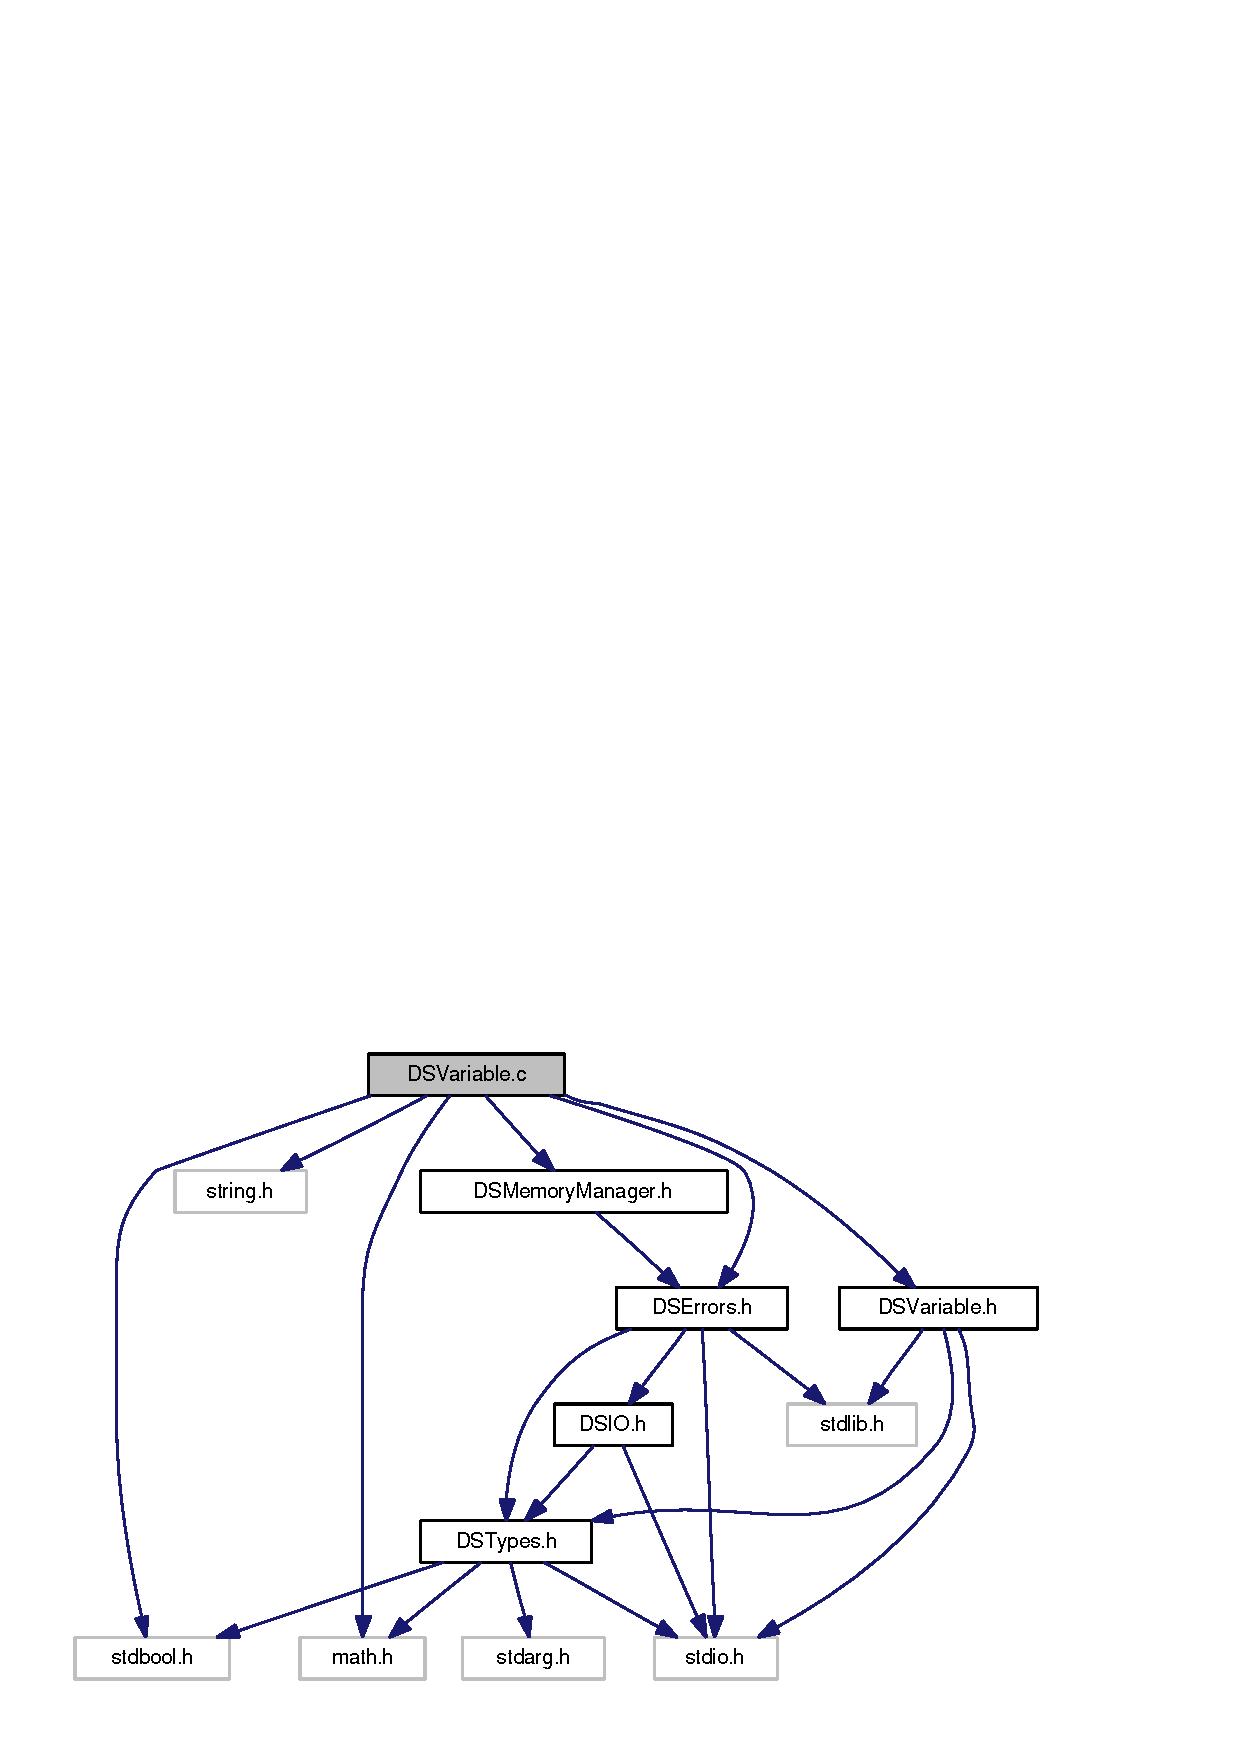
\includegraphics[width=258pt]{_d_s_variable_8c__incl}
\end{center}
\end{figure}
This graph shows which files directly or indirectly include this file:\subsection*{Functions}
\begin{DoxyCompactItemize}
\item 
\hyperlink{struct_d_s_variable}{DSVariable} $\ast$ \hyperlink{_d_s_variable_8c_a6f0ce189a8dc8ce46fad1d7a9b34d31f}{DSVariableAlloc} (const char $\ast$name)
\begin{DoxyCompactList}\small\item\em Creates a new \hyperlink{struct_d_s_variable}{DSVariable} with INFINITY as a default value. \item\end{DoxyCompactList}\item 
void \hyperlink{_d_s_variable_8c_aac8fadf2969493124be37a1076a2b885}{DSVariableFree} (\hyperlink{struct_d_s_variable}{DSVariable} $\ast$var)
\begin{DoxyCompactList}\small\item\em Function frees allocated memory of a \hyperlink{struct_d_s_variable}{DSVariable}. \item\end{DoxyCompactList}\item 
\hyperlink{struct_d_s_variable}{DSVariable} $\ast$ \hyperlink{_d_s_variable_8c_a1a5da69573335a86dea1e4a8a6770ea3}{DSVariableRetain} (\hyperlink{struct_d_s_variable}{DSVariable} $\ast$aVariable)
\begin{DoxyCompactList}\small\item\em Function to increase variable retain count by one. \item\end{DoxyCompactList}\item 
void \hyperlink{_d_s_variable_8c_a4d83eec85c4d9340593a359fd1d5e506}{DSVariableRelease} (\hyperlink{struct_d_s_variable}{DSVariable} $\ast$aVariable)
\begin{DoxyCompactList}\small\item\em Function to decrease variable retain count by one. \item\end{DoxyCompactList}\item 
\hyperlink{struct_d_s_variable_pool}{DSVariablePool} $\ast$ \hyperlink{_d_s_variable_8c_a1cff6b1af2bc3210cc65435c1844b5ef}{DSVariablePoolAlloc} (void)
\begin{DoxyCompactList}\small\item\em Creates a new \hyperlink{struct_d_s_variable_pool}{DSVariablePool} with an empty var dictionary. \item\end{DoxyCompactList}\item 
\hypertarget{_d_s_variable_8c_a11c76e0e57dbc00e57edb94b65ea0244}{
\hyperlink{struct_d_s_variable_pool}{DSVariablePool} $\ast$ {\bfseries DSVariablePoolCopy} (const \hyperlink{struct_d_s_variable_pool}{DSVariablePool} $\ast$const pool)}
\label{_d_s_variable_8c_a11c76e0e57dbc00e57edb94b65ea0244}

\item 
\hypertarget{_d_s_variable_8c_abe8cde590093cb49af32d532135d0d57}{
void {\bfseries DSVariablePoolFree} (\hyperlink{struct_d_s_variable_pool}{DSVariablePool} $\ast$pool)}
\label{_d_s_variable_8c_abe8cde590093cb49af32d532135d0d57}

\item 
\hypertarget{_d_s_variable_8c_a2ac568a1be064c51cffc7751776b4403}{
void {\bfseries DSVariablePoolSetReadOnly} (\hyperlink{struct_d_s_variable_pool}{DSVariablePool} $\ast$pool)}
\label{_d_s_variable_8c_a2ac568a1be064c51cffc7751776b4403}

\item 
\hypertarget{_d_s_variable_8c_a80e57736e4bf63d4d88ea2af79b8417e}{
void {\bfseries DSVariablePoolSetReadWrite} (\hyperlink{struct_d_s_variable_pool}{DSVariablePool} $\ast$pool)}
\label{_d_s_variable_8c_a80e57736e4bf63d4d88ea2af79b8417e}

\item 
\hypertarget{_d_s_variable_8c_a66afd8da098073ab4ef8c06e5d5257b8}{
void {\bfseries DSVariablePoolSetReadWriteAdd} (\hyperlink{struct_d_s_variable_pool}{DSVariablePool} $\ast$pool)}
\label{_d_s_variable_8c_a66afd8da098073ab4ef8c06e5d5257b8}

\item 
\hypertarget{_d_s_variable_8c_aaa1b27aad0f93b52cf615a57d77cb142}{
bool {\bfseries DSVariablePoolIsReadOnly} (const \hyperlink{struct_d_s_variable_pool}{DSVariablePool} $\ast$pool)}
\label{_d_s_variable_8c_aaa1b27aad0f93b52cf615a57d77cb142}

\item 
\hypertarget{_d_s_variable_8c_a7dc75250a954763bb8e9b217af50aa2f}{
bool {\bfseries DSVariablePoolIsReadWrite} (const \hyperlink{struct_d_s_variable_pool}{DSVariablePool} $\ast$pool)}
\label{_d_s_variable_8c_a7dc75250a954763bb8e9b217af50aa2f}

\item 
\hypertarget{_d_s_variable_8c_a9c6dcd1e5ec12a5cdd18df0fdb753ca9}{
bool {\bfseries DSVariablePoolIsReadWriteAdd} (const \hyperlink{struct_d_s_variable_pool}{DSVariablePool} $\ast$pool)}
\label{_d_s_variable_8c_a9c6dcd1e5ec12a5cdd18df0fdb753ca9}

\item 
\hypertarget{_d_s_variable_8c_a795b9def0c0cdd4fd1bd99dee0e18b24}{
void {\bfseries DSVariablePoolAddVariableWithName} (\hyperlink{struct_d_s_variable_pool}{DSVariablePool} $\ast$pool, const char $\ast$name)}
\label{_d_s_variable_8c_a795b9def0c0cdd4fd1bd99dee0e18b24}

\item 
\hypertarget{_d_s_variable_8c_aa9ecf8bde68b63daba6f83b95cb4a471}{
void {\bfseries DSVariablePoolAddVariable} (\hyperlink{struct_d_s_variable_pool}{DSVariablePool} $\ast$pool, \hyperlink{struct_d_s_variable}{DSVariable} $\ast$newVar)}
\label{_d_s_variable_8c_aa9ecf8bde68b63daba6f83b95cb4a471}

\item 
\hypertarget{_d_s_variable_8c_aa0ab405c594ec1e1ba47cd36703d8ae5}{
bool {\bfseries DSVariablePoolHasVariableWithName} (const \hyperlink{struct_d_s_variable_pool}{DSVariablePool} $\ast$pool, const char $\ast$const name)}
\label{_d_s_variable_8c_aa0ab405c594ec1e1ba47cd36703d8ae5}

\item 
\hypertarget{_d_s_variable_8c_a4d59ca020b7df35f9d7320147800dad0}{
\hyperlink{struct_d_s_variable}{DSVariable} $\ast$ {\bfseries DSVariablePoolVariableWithName} (const \hyperlink{struct_d_s_variable_pool}{DSVariablePool} $\ast$pool, const char $\ast$name)}
\label{_d_s_variable_8c_a4d59ca020b7df35f9d7320147800dad0}

\item 
\hypertarget{_d_s_variable_8c_aca1491d35e9f15e6a00783f58b9e7c6c}{
void {\bfseries DSVariablePoolSetValueForVariableWithName} (const \hyperlink{struct_d_s_variable_pool}{DSVariablePool} $\ast$pool, const char $\ast$name, const double value)}
\label{_d_s_variable_8c_aca1491d35e9f15e6a00783f58b9e7c6c}

\item 
\hypertarget{_d_s_variable_8c_a7c0345124038d444aa55c6210ac766f5}{
const \hyperlink{struct_d_s_variable}{DSVariable} $\ast$$\ast$ {\bfseries DSVariablePoolAllVariables} (const \hyperlink{struct_d_s_variable_pool}{DSVariablePool} $\ast$pool)}
\label{_d_s_variable_8c_a7c0345124038d444aa55c6210ac766f5}

\item 
\hypertarget{_d_s_variable_8c_a9c39f5fe68099e6df8008e154698a0e6}{
const char $\ast$$\ast$ {\bfseries DSVariablePoolAllVariableNames} (const \hyperlink{struct_d_s_variable_pool}{DSVariablePool} $\ast$pool)}
\label{_d_s_variable_8c_a9c39f5fe68099e6df8008e154698a0e6}

\item 
\hypertarget{_d_s_variable_8c_a958544604efb5e2f931b967dd3ab240d}{
DSUInteger {\bfseries DSVariablePoolIndexOfVariable} (const \hyperlink{struct_d_s_variable_pool}{DSVariablePool} $\ast$pool, const \hyperlink{struct_d_s_variable}{DSVariable} $\ast$var)}
\label{_d_s_variable_8c_a958544604efb5e2f931b967dd3ab240d}

\item 
\hypertarget{_d_s_variable_8c_afd887f623bb5e13694754097bc9c7b15}{
DSUInteger {\bfseries DSVariablePoolIndexOfVariableWithName} (const \hyperlink{struct_d_s_variable_pool}{DSVariablePool} $\ast$pool, const char $\ast$name)}
\label{_d_s_variable_8c_afd887f623bb5e13694754097bc9c7b15}

\item 
\hypertarget{_d_s_variable_8c_a0d21cf1b61f32965532d6bb86c8195d4}{
\hyperlink{struct_d_s_variable_pool}{DSVariablePool} $\ast$ {\bfseries DSVariablePoolByParsingString} (const char $\ast$string)}
\label{_d_s_variable_8c_a0d21cf1b61f32965532d6bb86c8195d4}

\item 
\hypertarget{_d_s_variable_8c_a1ee4a6e864741c90621174674032de5f}{
void {\bfseries DSVariablePoolPrint} (const \hyperlink{struct_d_s_variable_pool}{DSVariablePool} $\ast$const pool)}
\label{_d_s_variable_8c_a1ee4a6e864741c90621174674032de5f}

\item 
\hypertarget{_d_s_variable_8c_a96a40866627c87b8beb764f85106f6e9}{
\hyperlink{struct_d_s_matrix}{DSMatrix} $\ast$ {\bfseries DSVariablePoolValuesAsVector} (const \hyperlink{struct_d_s_variable_pool}{DSVariablePool} $\ast$pool, const bool rowVector)}
\label{_d_s_variable_8c_a96a40866627c87b8beb764f85106f6e9}

\end{DoxyCompactItemize}
\subsection*{Variables}
\begin{DoxyCompactItemize}
\item 
\hypertarget{_d_s_variable_8c_a6619150c9752c45d9a5577c5eea8fae6}{
pthread\_\-mutex\_\-t {\bfseries retaincount}}
\label{_d_s_variable_8c_a6619150c9752c45d9a5577c5eea8fae6}

\end{DoxyCompactItemize}


\subsection{Detailed Description}
Implementation file with functions for dealing with variables. Copyright (C) 2011 Jason Lomnitz.\par
\par


This file is part of the Design Space Toolbox V2 (C Library).

The Design Space Toolbox V2 is free software: you can redistribute it and/or modify it under the terms of the GNU General Public License as published by the Free Software Foundation, either version 3 of the License, or (at your option) any later version.

The Design Space Toolbox V2 is distributed in the hope that it will be useful, but WITHOUT ANY WARRANTY; without even the implied warranty of MERCHANTABILITY or FITNESS FOR A PARTICULAR PURPOSE. See the GNU General Public License for more details.

You should have received a copy of the GNU General Public License along with the Design Space Toolbox. If not, see $<$\href{http://www.gnu.org/licenses/}{\tt http://www.gnu.org/licenses/}$>$.

\begin{DoxyAuthor}{Author}
Jason Lomnitz. 
\end{DoxyAuthor}
\begin{DoxyDate}{Date}
2011 
\end{DoxyDate}


\subsection{Function Documentation}
\hypertarget{_d_s_variable_8c_a6f0ce189a8dc8ce46fad1d7a9b34d31f}{
\index{DSVariable.c@{DSVariable.c}!DSVariableAlloc@{DSVariableAlloc}}
\index{DSVariableAlloc@{DSVariableAlloc}!DSVariable.c@{DSVariable.c}}
\subsubsection[{DSVariableAlloc}]{\setlength{\rightskip}{0pt plus 5cm}{\bf DSVariable}$\ast$ DSVariableAlloc (const char $\ast$ {\em name})}}
\label{_d_s_variable_8c_a6f0ce189a8dc8ce46fad1d7a9b34d31f}


Creates a new \hyperlink{struct_d_s_variable}{DSVariable} with INFINITY as a default value. 

This function may be used throughout, in order to create new variables consistently and portably. As variables are allocated individually, it is important to not that they should be released with the accesory method. 
\begin{DoxyParams}{Parameters}
\item[{\em name}]A string with which to identify the \hyperlink{struct_d_s_variable}{DSVariable}. \end{DoxyParams}
\begin{DoxyReturn}{Returns}
The pointer to the newly allocated \hyperlink{struct_d_s_variable}{DSVariable}. 
\end{DoxyReturn}
\begin{DoxySeeAlso}{See also}
\hyperlink{struct_d_s_variable}{DSVariable} 

\hyperlink{_d_s_variable_8h_aac8fadf2969493124be37a1076a2b885}{DSVariableFree} 
\end{DoxySeeAlso}
\hypertarget{_d_s_variable_8c_aac8fadf2969493124be37a1076a2b885}{
\index{DSVariable.c@{DSVariable.c}!DSVariableFree@{DSVariableFree}}
\index{DSVariableFree@{DSVariableFree}!DSVariable.c@{DSVariable.c}}
\subsubsection[{DSVariableFree}]{\setlength{\rightskip}{0pt plus 5cm}void DSVariableFree ({\bf DSVariable} $\ast$ {\em var})}}
\label{_d_s_variable_8c_aac8fadf2969493124be37a1076a2b885}


Function frees allocated memory of a \hyperlink{struct_d_s_variable}{DSVariable}. 

This function should be used for each newDSVariable that is called. The internal structure is subject to changes in consequent versions and therefore freeing memory of DSVariables should be strictly through this function. 
\begin{DoxyParams}{Parameters}
\item[{\em var}]The pointer to the variable to free. \end{DoxyParams}
\hypertarget{_d_s_variable_8c_a1cff6b1af2bc3210cc65435c1844b5ef}{
\index{DSVariable.c@{DSVariable.c}!DSVariablePoolAlloc@{DSVariablePoolAlloc}}
\index{DSVariablePoolAlloc@{DSVariablePoolAlloc}!DSVariable.c@{DSVariable.c}}
\subsubsection[{DSVariablePoolAlloc}]{\setlength{\rightskip}{0pt plus 5cm}{\bf DSVariablePool}$\ast$ DSVariablePoolAlloc (void)}}
\label{_d_s_variable_8c_a1cff6b1af2bc3210cc65435c1844b5ef}


Creates a new \hyperlink{struct_d_s_variable_pool}{DSVariablePool} with an empty var dictionary. 

The variable pool is initialized with read/write privilages. The variable pool stores a indexed version of the variables added, as well as the order in which the variables were added. The order of the variables is kept to ensure a consistent variable index with system matrices of S-\/Systems and GMAs.

\begin{DoxyReturn}{Returns}
The pointer to the allocated \hyperlink{struct_d_s_variable_pool}{DSVariablePool}.
\end{DoxyReturn}
\begin{DoxySeeAlso}{See also}
DSVariablePoolFree 
\end{DoxySeeAlso}
\hypertarget{_d_s_variable_8c_a4d83eec85c4d9340593a359fd1d5e506}{
\index{DSVariable.c@{DSVariable.c}!DSVariableRelease@{DSVariableRelease}}
\index{DSVariableRelease@{DSVariableRelease}!DSVariable.c@{DSVariable.c}}
\subsubsection[{DSVariableRelease}]{\setlength{\rightskip}{0pt plus 5cm}void DSVariableRelease ({\bf DSVariable} $\ast$ {\em aVariable})}}
\label{_d_s_variable_8c_a4d83eec85c4d9340593a359fd1d5e506}


Function to decrease variable retain count by one. 

Fast processing tree is made to decrease its retain count by one, when the retain count hits zero, the function \hyperlink{_d_s_variable_8c_aac8fadf2969493124be37a1076a2b885}{DSVariableFree()} is invoked, freeing the memory space. Fast processing tree does not have an equivalent to autorelease, forcing the developer to use greater care when directly managing memory.


\begin{DoxyParams}{Parameters}
\item[{\em aVariable}]The variable which will have its retain count reduced.\end{DoxyParams}
\begin{DoxySeeAlso}{See also}
\hyperlink{_d_s_variable_8h_a1a5da69573335a86dea1e4a8a6770ea3}{DSVariableRetain} 

\hyperlink{_d_s_variable_8h_aac8fadf2969493124be37a1076a2b885}{DSVariableFree} 
\end{DoxySeeAlso}
\hypertarget{_d_s_variable_8c_a1a5da69573335a86dea1e4a8a6770ea3}{
\index{DSVariable.c@{DSVariable.c}!DSVariableRetain@{DSVariableRetain}}
\index{DSVariableRetain@{DSVariableRetain}!DSVariable.c@{DSVariable.c}}
\subsubsection[{DSVariableRetain}]{\setlength{\rightskip}{0pt plus 5cm}{\bf DSVariable}$\ast$ DSVariableRetain ({\bf DSVariable} $\ast$ {\em aVariable})}}
\label{_d_s_variable_8c_a1a5da69573335a86dea1e4a8a6770ea3}


Function to increase variable retain count by one. 

Variables utilize a similar memory management system used in Objective-\/C NSObject subclasses, where objects a retained/released.


\begin{DoxyParams}{Parameters}
\item[{\em aVariable}]The variable which will have its retain count increased.\end{DoxyParams}
\begin{DoxyReturn}{Returns}
The same variable which received the retain count increase is returned, for convinience.
\end{DoxyReturn}
\begin{DoxySeeAlso}{See also}
\hyperlink{_d_s_variable_8h_a4d83eec85c4d9340593a359fd1d5e506}{DSVariableRelease} 
\end{DoxySeeAlso}

\hypertarget{_d_s_variable_8h}{
\section{DSVariable.h File Reference}
\label{_d_s_variable_8h}\index{DSVariable.h@{DSVariable.h}}
}


Header file with functions for dealing with variables.  


{\ttfamily \#include $<$stdio.h$>$}\par
{\ttfamily \#include $<$stdlib.h$>$}\par
{\ttfamily \#include \char`\"{}DSTypes.h\char`\"{}}\par
{\ttfamily \#include \char`\"{}DSDictionary.h\char`\"{}}\par
Include dependency graph for DSVariable.h:\nopagebreak
\begin{figure}[H]
\begin{center}
\leavevmode
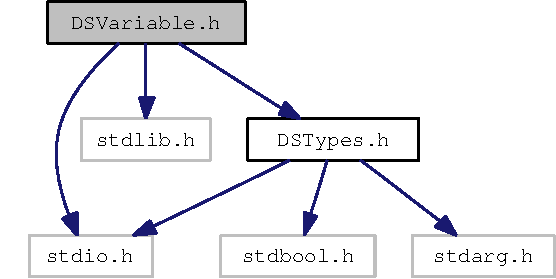
\includegraphics[width=175pt]{_d_s_variable_8h__incl}
\end{center}
\end{figure}
This graph shows which files directly or indirectly include this file:\nopagebreak
\begin{figure}[H]
\begin{center}
\leavevmode
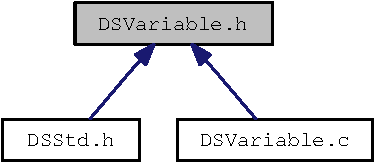
\includegraphics[width=65pt]{_d_s_variable_8h__dep__incl}
\end{center}
\end{figure}
\subsection*{Defines}
\begin{DoxyCompactItemize}
\item 
\hypertarget{_d_s_variable_8h_a3e1730e26b5f44a34e64d7996233d023}{
\#define {\bfseries DSVariableAssignValue}(x, y)~DSVariableSetValue(x, y)}
\label{_d_s_variable_8h_a3e1730e26b5f44a34e64d7996233d023}

\item 
\hypertarget{_d_s_variable_8h_a912df8d84202953a573824aebcf2498f}{
\#define {\bfseries DSVariableReturnValue}(x)~DSVariableValue(x)}
\label{_d_s_variable_8h_a912df8d84202953a573824aebcf2498f}

\item 
\#define \hyperlink{group___d_s___v_a_r_i_a_b_l_e___a_c_c_e_s_s_o_r_y_ga218a0d1de0bb5ea62d7e5aa22fe50793}{DSVariableSetValue}(x, y)~(((\hyperlink{struct_d_s_variable}{DSVariable}$\ast$)(x))-\/$>$value = (y))
\begin{DoxyCompactList}\small\item\em Macro to set the value of a variable data structure. \item\end{DoxyCompactList}\item 
\#define \hyperlink{group___d_s___v_a_r_i_a_b_l_e___a_c_c_e_s_s_o_r_y_ga837d0718b28591df6f518eb50d98082a}{DSVariableValue}(x)~(((x) != NULL) ? ((\hyperlink{struct_d_s_variable}{DSVariable}$\ast$)x)-\/$>$value : NAN)
\begin{DoxyCompactList}\small\item\em Macro to get the value of a variable data structure. \item\end{DoxyCompactList}\item 
\#define \hyperlink{group___d_s___v_a_r_i_a_b_l_e___a_c_c_e_s_s_o_r_y_ga64afbf5e8e378ef611c25084211152c4}{DSVariableName}(x)~(((\hyperlink{struct_d_s_variable}{DSVariable} $\ast$)x)-\/$>$name)
\begin{DoxyCompactList}\small\item\em Macro to get the value of a variable data structure. \item\end{DoxyCompactList}\item 
\hypertarget{group___m___d_s___messages_gac31f10e693824b630ea7bd80f59acadf}{
\#define \hyperlink{group___m___d_s___messages_gac31f10e693824b630ea7bd80f59acadf}{M\_\-DS\_\-VAR\_\-NULL}~M\_\-DS\_\-NULL \char`\"{}: Variable Pool is NULL\char`\"{}}
\label{group___m___d_s___messages_gac31f10e693824b630ea7bd80f59acadf}

\begin{DoxyCompactList}\small\item\em Error message indicating a NULL variable pool. \item\end{DoxyCompactList}\item 
\hypertarget{group___m___d_s___messages_gaa3430366ad7beeafb53737b0174c5a0b}{
\#define \hyperlink{group___m___d_s___messages_gaa3430366ad7beeafb53737b0174c5a0b}{M\_\-DS\_\-VAR\_\-LOCKED}~\char`\"{} DSVariablePool: Insufficient priviliges\char`\"{}}
\label{group___m___d_s___messages_gaa3430366ad7beeafb53737b0174c5a0b}

\begin{DoxyCompactList}\small\item\em Error message indicating insufficient priviliges to manipulate a variable pool. \item\end{DoxyCompactList}\item 
\hypertarget{_d_s_variable_8h_a2eba27e3c90e74233f65a3737cf82070}{
\#define {\bfseries DSVariablePoolInternalDictionary}(x)~((x)-\/$>$dictionary)}
\label{_d_s_variable_8h_a2eba27e3c90e74233f65a3737cf82070}

\item 
\hypertarget{_d_s_variable_8h_a9e51b74e2041e6ca9bafd73ce156edce}{
\#define {\bfseries DSVariablePoolVariableArray}(x)~((x)-\/$>$variables)}
\label{_d_s_variable_8h_a9e51b74e2041e6ca9bafd73ce156edce}

\end{DoxyCompactItemize}
\subsection*{Functions}
\begin{DoxyCompactItemize}
\item 
\hyperlink{struct_d_s_variable}{DSVariable} $\ast$ \hyperlink{_d_s_variable_8h_a6f0ce189a8dc8ce46fad1d7a9b34d31f}{DSVariableAlloc} (const char $\ast$name)
\begin{DoxyCompactList}\small\item\em Creates a new \hyperlink{struct_d_s_variable}{DSVariable} with INFINITY as a default value. \item\end{DoxyCompactList}\item 
void \hyperlink{_d_s_variable_8h_aac8fadf2969493124be37a1076a2b885}{DSVariableFree} (\hyperlink{struct_d_s_variable}{DSVariable} $\ast$var)
\begin{DoxyCompactList}\small\item\em Function frees allocated memory of a \hyperlink{struct_d_s_variable}{DSVariable}. \item\end{DoxyCompactList}\item 
\hyperlink{struct_d_s_variable}{DSVariable} $\ast$ \hyperlink{_d_s_variable_8h_a1a5da69573335a86dea1e4a8a6770ea3}{DSVariableRetain} (\hyperlink{struct_d_s_variable}{DSVariable} $\ast$aVariable)
\begin{DoxyCompactList}\small\item\em Function to increase variable retain count by one. \item\end{DoxyCompactList}\item 
void \hyperlink{_d_s_variable_8h_a4d83eec85c4d9340593a359fd1d5e506}{DSVariableRelease} (\hyperlink{struct_d_s_variable}{DSVariable} $\ast$aVariable)
\begin{DoxyCompactList}\small\item\em Function to decrease variable retain count by one. \item\end{DoxyCompactList}\item 
\hyperlink{struct_d_s_variable_pool}{DSVariablePool} $\ast$ \hyperlink{_d_s_variable_8h_a1cff6b1af2bc3210cc65435c1844b5ef}{DSVariablePoolAlloc} (void)
\begin{DoxyCompactList}\small\item\em Creates a new \hyperlink{struct_d_s_variable_pool}{DSVariablePool} with an empty var dictionary. \item\end{DoxyCompactList}\item 
\hyperlink{struct_d_s_variable_pool}{DSVariablePool} $\ast$ \hyperlink{_d_s_variable_8h_a11c76e0e57dbc00e57edb94b65ea0244}{DSVariablePoolCopy} (const \hyperlink{struct_d_s_variable_pool}{DSVariablePool} $\ast$const pool)
\begin{DoxyCompactList}\small\item\em Creates a new \hyperlink{struct_d_s_variable_pool}{DSVariablePool} with a copy of the reference variable pool. \item\end{DoxyCompactList}\item 
void \hyperlink{_d_s_variable_8h_abe8cde590093cb49af32d532135d0d57}{DSVariablePoolFree} (\hyperlink{struct_d_s_variable_pool}{DSVariablePool} $\ast$pool)
\begin{DoxyCompactList}\small\item\em Creates a new \hyperlink{struct_d_s_variable_pool}{DSVariablePool} with a copy of the reference variable pool. \item\end{DoxyCompactList}\item 
\hypertarget{_d_s_variable_8h_a0d21cf1b61f32965532d6bb86c8195d4}{
\hyperlink{struct_d_s_variable_pool}{DSVariablePool} $\ast$ {\bfseries DSVariablePoolByParsingString} (const char $\ast$string)}
\label{_d_s_variable_8h_a0d21cf1b61f32965532d6bb86c8195d4}

\item 
void \hyperlink{_d_s_variable_8h_a2ac568a1be064c51cffc7751776b4403}{DSVariablePoolSetReadOnly} (\hyperlink{struct_d_s_variable_pool}{DSVariablePool} $\ast$pool)
\begin{DoxyCompactList}\small\item\em Changes the existing priviliges of a \hyperlink{struct_d_s_variable_pool}{DSVariablePool} object to read only. \item\end{DoxyCompactList}\item 
void \hyperlink{_d_s_variable_8h_a80e57736e4bf63d4d88ea2af79b8417e}{DSVariablePoolSetReadWrite} (\hyperlink{struct_d_s_variable_pool}{DSVariablePool} $\ast$pool)
\begin{DoxyCompactList}\small\item\em Changes the existing priviliges of a \hyperlink{struct_d_s_variable_pool}{DSVariablePool} object to read and write. \item\end{DoxyCompactList}\item 
void \hyperlink{_d_s_variable_8h_a66afd8da098073ab4ef8c06e5d5257b8}{DSVariablePoolSetReadWriteAdd} (\hyperlink{struct_d_s_variable_pool}{DSVariablePool} $\ast$pool)
\begin{DoxyCompactList}\small\item\em Changes the existing priviliges of a \hyperlink{struct_d_s_variable_pool}{DSVariablePool} object to read, write and add. \item\end{DoxyCompactList}\item 
void \hyperlink{_d_s_variable_8h_a795b9def0c0cdd4fd1bd99dee0e18b24}{DSVariablePoolAddVariableWithName} (\hyperlink{struct_d_s_variable_pool}{DSVariablePool} $\ast$pool, const char $\ast$name)
\begin{DoxyCompactList}\small\item\em Creates and adds a new variable to the variable pool. \item\end{DoxyCompactList}\item 
void \hyperlink{_d_s_variable_8h_aa9ecf8bde68b63daba6f83b95cb4a471}{DSVariablePoolAddVariable} (\hyperlink{struct_d_s_variable_pool}{DSVariablePool} $\ast$pool, \hyperlink{struct_d_s_variable}{DSVariable} $\ast$newVar)
\begin{DoxyCompactList}\small\item\em Adds an existing variable to the variable pool. \item\end{DoxyCompactList}\item 
\hypertarget{_d_s_variable_8h_aca1491d35e9f15e6a00783f58b9e7c6c}{
void {\bfseries DSVariablePoolSetValueForVariableWithName} (const \hyperlink{struct_d_s_variable_pool}{DSVariablePool} $\ast$pool, const char $\ast$name, const double value)}
\label{_d_s_variable_8h_aca1491d35e9f15e6a00783f58b9e7c6c}

\item 
DSUInteger \hyperlink{_d_s_variable_8h_a40cc4676d919ffddc43afb1d91cc31b5}{DSVariablePoolNumberOfVariables} (const \hyperlink{struct_d_s_variable_pool}{DSVariablePool} $\ast$pool)
\begin{DoxyCompactList}\small\item\em Function to retrieve the number of variables in a \hyperlink{struct_d_s_variable_pool}{DSVariablePool}. \item\end{DoxyCompactList}\item 
bool \hyperlink{_d_s_variable_8h_aaa1b27aad0f93b52cf615a57d77cb142}{DSVariablePoolIsReadOnly} (const \hyperlink{struct_d_s_variable_pool}{DSVariablePool} $\ast$pool)
\begin{DoxyCompactList}\small\item\em Queries the existing priviliges of a \hyperlink{struct_d_s_variable_pool}{DSVariablePool} object, checking it is read only. \item\end{DoxyCompactList}\item 
bool \hyperlink{_d_s_variable_8h_a7dc75250a954763bb8e9b217af50aa2f}{DSVariablePoolIsReadWrite} (const \hyperlink{struct_d_s_variable_pool}{DSVariablePool} $\ast$pool)
\begin{DoxyCompactList}\small\item\em Queries the existing priviliges of a \hyperlink{struct_d_s_variable_pool}{DSVariablePool} object, checking it is read and write. \item\end{DoxyCompactList}\item 
bool \hyperlink{_d_s_variable_8h_a9c6dcd1e5ec12a5cdd18df0fdb753ca9}{DSVariablePoolIsReadWriteAdd} (const \hyperlink{struct_d_s_variable_pool}{DSVariablePool} $\ast$pool)
\begin{DoxyCompactList}\small\item\em Queries the existing priviliges of a \hyperlink{struct_d_s_variable_pool}{DSVariablePool} object, checking it is read, write and add. \item\end{DoxyCompactList}\item 
\hypertarget{_d_s_variable_8h_aa0ab405c594ec1e1ba47cd36703d8ae5}{
bool \hyperlink{_d_s_variable_8h_aa0ab405c594ec1e1ba47cd36703d8ae5}{DSVariablePoolHasVariableWithName} (const \hyperlink{struct_d_s_variable_pool}{DSVariablePool} $\ast$pool, const char $\ast$const name)}
\label{_d_s_variable_8h_aa0ab405c594ec1e1ba47cd36703d8ae5}

\begin{DoxyCompactList}\small\item\em Checks if a \hyperlink{struct_d_s_variable_pool}{DSVariablePool} has a variable with a specified name. \item\end{DoxyCompactList}\item 
\hypertarget{_d_s_variable_8h_a4d59ca020b7df35f9d7320147800dad0}{
\hyperlink{struct_d_s_variable}{DSVariable} $\ast$ {\bfseries DSVariablePoolVariableWithName} (const \hyperlink{struct_d_s_variable_pool}{DSVariablePool} $\ast$pool, const char $\ast$name)}
\label{_d_s_variable_8h_a4d59ca020b7df35f9d7320147800dad0}

\item 
\hypertarget{_d_s_variable_8h_af2adea119e062ca1932c50808785e667}{
const \hyperlink{struct_d_s_variable}{DSVariable} $\ast$ {\bfseries DSVariablePoolVariableAtIndex} (const \hyperlink{struct_d_s_variable_pool}{DSVariablePool} $\ast$pool, const DSUInteger index)}
\label{_d_s_variable_8h_af2adea119e062ca1932c50808785e667}

\item 
\hypertarget{_d_s_variable_8h_a7d7984c84d2d9617f408310d342d02a3}{
double {\bfseries DSVariablePoolValueForVariableWithName} (const \hyperlink{struct_d_s_variable_pool}{DSVariablePool} $\ast$pool, const char const $\ast$name)}
\label{_d_s_variable_8h_a7d7984c84d2d9617f408310d342d02a3}

\item 
\hypertarget{_d_s_variable_8h_a78241cc765be0432f0c6e9eb21b42782}{
const \hyperlink{struct_d_s_variable}{DSVariable} $\ast$$\ast$ {\bfseries DSVariablePoolAllVariables} (const \hyperlink{struct_d_s_variable_pool}{DSVariablePool} $\ast$pool)}
\label{_d_s_variable_8h_a78241cc765be0432f0c6e9eb21b42782}

\item 
\hypertarget{_d_s_variable_8h_a9c39f5fe68099e6df8008e154698a0e6}{
const char $\ast$$\ast$ {\bfseries DSVariablePoolAllVariableNames} (const \hyperlink{struct_d_s_variable_pool}{DSVariablePool} $\ast$pool)}
\label{_d_s_variable_8h_a9c39f5fe68099e6df8008e154698a0e6}

\item 
\hypertarget{_d_s_variable_8h_a958544604efb5e2f931b967dd3ab240d}{
DSUInteger {\bfseries DSVariablePoolIndexOfVariable} (const \hyperlink{struct_d_s_variable_pool}{DSVariablePool} $\ast$pool, const \hyperlink{struct_d_s_variable}{DSVariable} $\ast$var)}
\label{_d_s_variable_8h_a958544604efb5e2f931b967dd3ab240d}

\item 
\hypertarget{_d_s_variable_8h_afd887f623bb5e13694754097bc9c7b15}{
DSUInteger {\bfseries DSVariablePoolIndexOfVariableWithName} (const \hyperlink{struct_d_s_variable_pool}{DSVariablePool} $\ast$pool, const char $\ast$name)}
\label{_d_s_variable_8h_afd887f623bb5e13694754097bc9c7b15}

\item 
\hypertarget{_d_s_variable_8h_a1ee4a6e864741c90621174674032de5f}{
void {\bfseries DSVariablePoolPrint} (const \hyperlink{struct_d_s_variable_pool}{DSVariablePool} $\ast$const pool)}
\label{_d_s_variable_8h_a1ee4a6e864741c90621174674032de5f}

\item 
\hypertarget{_d_s_variable_8h_a96a40866627c87b8beb764f85106f6e9}{
\hyperlink{struct_d_s_matrix}{DSMatrix} $\ast$ {\bfseries DSVariablePoolValuesAsVector} (const \hyperlink{struct_d_s_variable_pool}{DSVariablePool} $\ast$pool, const bool rowVector)}
\label{_d_s_variable_8h_a96a40866627c87b8beb764f85106f6e9}

\end{DoxyCompactItemize}


\subsection{Detailed Description}
Header file with functions for dealing with variables. Copyright (C) 2011 Jason Lomnitz.\par
\par


This file is part of the Design Space Toolbox V2 (C Library).

The Design Space Toolbox V2 is free software: you can redistribute it and/or modify it under the terms of the GNU General Public License as published by the Free Software Foundation, either version 3 of the License, or (at your option) any later version.

The Design Space Toolbox V2 is distributed in the hope that it will be useful, but WITHOUT ANY WARRANTY; without even the implied warranty of MERCHANTABILITY or FITNESS FOR A PARTICULAR PURPOSE. See the GNU General Public License for more details.

You should have received a copy of the GNU General Public License along with the Design Space Toolbox. If not, see $<$\href{http://www.gnu.org/licenses/}{\tt http://www.gnu.org/licenses/}$>$.

\begin{DoxyAuthor}{Author}
Jason Lomnitz. 
\end{DoxyAuthor}
\begin{DoxyDate}{Date}
2011 
\end{DoxyDate}


\subsection{Function Documentation}
\hypertarget{_d_s_variable_8h_a6f0ce189a8dc8ce46fad1d7a9b34d31f}{
\index{DSVariable.h@{DSVariable.h}!DSVariableAlloc@{DSVariableAlloc}}
\index{DSVariableAlloc@{DSVariableAlloc}!DSVariable.h@{DSVariable.h}}
\subsubsection[{DSVariableAlloc}]{\setlength{\rightskip}{0pt plus 5cm}{\bf DSVariable}$\ast$ DSVariableAlloc (const char $\ast$ {\em name})}}
\label{_d_s_variable_8h_a6f0ce189a8dc8ce46fad1d7a9b34d31f}


Creates a new \hyperlink{struct_d_s_variable}{DSVariable} with INFINITY as a default value. 

This function may be used throughout, in order to create new variables consistently and portably. As variables are allocated individually, it is important to not that they should be released with the accesory method. 
\begin{DoxyParams}{Parameters}
\item[{\em name}]A string with which to identify the \hyperlink{struct_d_s_variable}{DSVariable}. \end{DoxyParams}
\begin{DoxyReturn}{Returns}
The pointer to the newly allocated \hyperlink{struct_d_s_variable}{DSVariable}. 
\end{DoxyReturn}
\begin{DoxySeeAlso}{See also}
\hyperlink{struct_d_s_variable}{DSVariable} 

\hyperlink{_d_s_variable_8h_aac8fadf2969493124be37a1076a2b885}{DSVariableFree} 
\end{DoxySeeAlso}
\hypertarget{_d_s_variable_8h_aac8fadf2969493124be37a1076a2b885}{
\index{DSVariable.h@{DSVariable.h}!DSVariableFree@{DSVariableFree}}
\index{DSVariableFree@{DSVariableFree}!DSVariable.h@{DSVariable.h}}
\subsubsection[{DSVariableFree}]{\setlength{\rightskip}{0pt plus 5cm}void DSVariableFree ({\bf DSVariable} $\ast$ {\em var})}}
\label{_d_s_variable_8h_aac8fadf2969493124be37a1076a2b885}


Function frees allocated memory of a \hyperlink{struct_d_s_variable}{DSVariable}. 

This function should not be used explicitly, as the \hyperlink{struct_d_s_variable}{DSVariable} object has an internal memory counter. This function is ultimately called when the variable memory counter reaches zero. Freeing a \hyperlink{struct_d_s_variable}{DSVariable} object should be done through the DSVariableRelease function, and never should a \hyperlink{struct_d_s_variable}{DSVariable} be directly freed, as its internal structure may be subject to future changes.


\begin{DoxyParams}{Parameters}
\item[{\em var}]The pointer to the variable to free.\end{DoxyParams}
\begin{DoxySeeAlso}{See also}
\hyperlink{_d_s_variable_8c_a1a5da69573335a86dea1e4a8a6770ea3}{DSVariableRetain()} 

\hyperlink{_d_s_variable_8c_a4d83eec85c4d9340593a359fd1d5e506}{DSVariableRelease()} 
\end{DoxySeeAlso}
\hypertarget{_d_s_variable_8h_aa9ecf8bde68b63daba6f83b95cb4a471}{
\index{DSVariable.h@{DSVariable.h}!DSVariablePoolAddVariable@{DSVariablePoolAddVariable}}
\index{DSVariablePoolAddVariable@{DSVariablePoolAddVariable}!DSVariable.h@{DSVariable.h}}
\subsubsection[{DSVariablePoolAddVariable}]{\setlength{\rightskip}{0pt plus 5cm}void DSVariablePoolAddVariable ({\bf DSVariablePool} $\ast$ {\em pool}, \/  {\bf DSVariable} $\ast$ {\em newVar})}}
\label{_d_s_variable_8h_aa9ecf8bde68b63daba6f83b95cb4a471}


Adds an existing variable to the variable pool. 

This function acts on an existing \hyperlink{struct_d_s_variable_pool}{DSVariablePool} object, adding an existing variable with a specified name to the internal dictionary structure. The variable added is not created, but this function calls DSVariableRetain, thus increasing the memory retain count of the variable by one. If a variable already exists with the same name, this function does not add the variable to the pool, and throws a warning.


\begin{DoxyParams}{Parameters}
\item[{\em pool}]The \hyperlink{struct_d_s_variable_pool}{DSVariablePool} object to which a new variable will be added. \item[{\em name}]A null terminated string with the name of the variable to add.\end{DoxyParams}
\begin{DoxySeeAlso}{See also}
\hyperlink{_d_s_variable_8c_a795b9def0c0cdd4fd1bd99dee0e18b24}{DSVariablePoolAddVariableWithName()} 

\hyperlink{_d_s_variable_8c_a1a5da69573335a86dea1e4a8a6770ea3}{DSVariableRetain()} 
\end{DoxySeeAlso}
\hypertarget{_d_s_variable_8h_a795b9def0c0cdd4fd1bd99dee0e18b24}{
\index{DSVariable.h@{DSVariable.h}!DSVariablePoolAddVariableWithName@{DSVariablePoolAddVariableWithName}}
\index{DSVariablePoolAddVariableWithName@{DSVariablePoolAddVariableWithName}!DSVariable.h@{DSVariable.h}}
\subsubsection[{DSVariablePoolAddVariableWithName}]{\setlength{\rightskip}{0pt plus 5cm}void DSVariablePoolAddVariableWithName ({\bf DSVariablePool} $\ast$ {\em pool}, \/  const char $\ast$ {\em name})}}
\label{_d_s_variable_8h_a795b9def0c0cdd4fd1bd99dee0e18b24}


Creates and adds a new variable to the variable pool. 

This function acts on an existing \hyperlink{struct_d_s_variable_pool}{DSVariablePool} object, creating a new variable with a specified name and adding it to the internal dictionary structure. If a variable already exists with the same name, this function does not create a new variable, and throws a warning.


\begin{DoxyParams}{Parameters}
\item[{\em pool}]The \hyperlink{struct_d_s_variable_pool}{DSVariablePool} object to which a new variable will be added. \item[{\em name}]A null terminated string with the name of the variable to add. \end{DoxyParams}
\hypertarget{_d_s_variable_8h_a1cff6b1af2bc3210cc65435c1844b5ef}{
\index{DSVariable.h@{DSVariable.h}!DSVariablePoolAlloc@{DSVariablePoolAlloc}}
\index{DSVariablePoolAlloc@{DSVariablePoolAlloc}!DSVariable.h@{DSVariable.h}}
\subsubsection[{DSVariablePoolAlloc}]{\setlength{\rightskip}{0pt plus 5cm}{\bf DSVariablePool}$\ast$ DSVariablePoolAlloc (void)}}
\label{_d_s_variable_8h_a1cff6b1af2bc3210cc65435c1844b5ef}


Creates a new \hyperlink{struct_d_s_variable_pool}{DSVariablePool} with an empty var dictionary. 

The variable pool is initialized with read/write privilages. The variable pool stores a indexed version of the variables added, as well as the order in which the variables were added. The order of the variables is kept to ensure a consistent variable index with system matrices of S-\/Systems and GMAs.

\begin{DoxyReturn}{Returns}
The pointer to the allocated \hyperlink{struct_d_s_variable_pool}{DSVariablePool}.
\end{DoxyReturn}
\begin{DoxySeeAlso}{See also}
\hyperlink{_d_s_variable_8h_abe8cde590093cb49af32d532135d0d57}{DSVariablePoolFree} 
\end{DoxySeeAlso}
\hypertarget{_d_s_variable_8h_a11c76e0e57dbc00e57edb94b65ea0244}{
\index{DSVariable.h@{DSVariable.h}!DSVariablePoolCopy@{DSVariablePoolCopy}}
\index{DSVariablePoolCopy@{DSVariablePoolCopy}!DSVariable.h@{DSVariable.h}}
\subsubsection[{DSVariablePoolCopy}]{\setlength{\rightskip}{0pt plus 5cm}{\bf DSVariablePool}$\ast$ DSVariablePoolCopy (const {\bf DSVariablePool} $\ast$const  {\em reference})}}
\label{_d_s_variable_8h_a11c76e0e57dbc00e57edb94b65ea0244}


Creates a new \hyperlink{struct_d_s_variable_pool}{DSVariablePool} with a copy of the reference variable pool. 

The variable pool that is created is initialized with the same read/write/add priviliges as the reference variable pool. The contents of the variable pool are an exact copy of the reference variable pool. Despite the contents being the same, the variables in each pool are independent, thus new variables are created in the copy.


\begin{DoxyParams}{Parameters}
\item[{\em reference}]A \hyperlink{struct_d_s_variable_pool}{DSVariablePool} data type that serves as the reference variable pool, which is to be copied.\end{DoxyParams}
\begin{DoxyReturn}{Returns}
The copy of the reference \hyperlink{struct_d_s_variable_pool}{DSVariablePool} object (must be freed by user).
\end{DoxyReturn}
\begin{DoxySeeAlso}{See also}
\hyperlink{_d_s_variable_8c_abe8cde590093cb49af32d532135d0d57}{DSVariablePoolFree()} 
\end{DoxySeeAlso}
\hypertarget{_d_s_variable_8h_abe8cde590093cb49af32d532135d0d57}{
\index{DSVariable.h@{DSVariable.h}!DSVariablePoolFree@{DSVariablePoolFree}}
\index{DSVariablePoolFree@{DSVariablePoolFree}!DSVariable.h@{DSVariable.h}}
\subsubsection[{DSVariablePoolFree}]{\setlength{\rightskip}{0pt plus 5cm}void DSVariablePoolFree ({\bf DSVariablePool} $\ast$ {\em pool})}}
\label{_d_s_variable_8h_abe8cde590093cb49af32d532135d0d57}


Creates a new \hyperlink{struct_d_s_variable_pool}{DSVariablePool} with a copy of the reference variable pool. 

The variable pool that is created is initialized with the same read/write/add priviliges as the reference variable pool. The contents of the variable pool are an exact copy of the reference variable pool. Despite the contents being the same, the variables in each pool are independent, thus new variables are created in the copy.


\begin{DoxyParams}{Parameters}
\item[{\em reference}]A \hyperlink{struct_d_s_variable_pool}{DSVariablePool} data type that serves as the reference variable pool, which is to be copied.\end{DoxyParams}
\begin{DoxyReturn}{Returns}
The copy of the reference \hyperlink{struct_d_s_variable_pool}{DSVariablePool} object (must be freed by user).
\end{DoxyReturn}
\begin{DoxySeeAlso}{See also}
\hyperlink{_d_s_variable_8c_abe8cde590093cb49af32d532135d0d57}{DSVariablePoolFree()} 
\end{DoxySeeAlso}
\hypertarget{_d_s_variable_8h_aaa1b27aad0f93b52cf615a57d77cb142}{
\index{DSVariable.h@{DSVariable.h}!DSVariablePoolIsReadOnly@{DSVariablePoolIsReadOnly}}
\index{DSVariablePoolIsReadOnly@{DSVariablePoolIsReadOnly}!DSVariable.h@{DSVariable.h}}
\subsubsection[{DSVariablePoolIsReadOnly}]{\setlength{\rightskip}{0pt plus 5cm}bool DSVariablePoolIsReadOnly (const {\bf DSVariablePool} $\ast$ {\em pool})}}
\label{_d_s_variable_8h_aaa1b27aad0f93b52cf615a57d77cb142}


Queries the existing priviliges of a \hyperlink{struct_d_s_variable_pool}{DSVariablePool} object, checking it is read only. 

This function acts on an existing \hyperlink{struct_d_s_variable_pool}{DSVariablePool} object, and checks if its priviliges are read only.


\begin{DoxyParams}{Parameters}
\item[{\em pool}]A \hyperlink{struct_d_s_variable_pool}{DSVariablePool} object to be queried for its priviliges.\end{DoxyParams}
\begin{DoxySeeAlso}{See also}
\hyperlink{_d_s_variable_8c_a7dc75250a954763bb8e9b217af50aa2f}{DSVariablePoolIsReadWrite()} 

\hyperlink{_d_s_variable_8c_a9c6dcd1e5ec12a5cdd18df0fdb753ca9}{DSVariablePoolIsReadWriteAdd()} 

\hyperlink{_d_s_types_8h_a62ad4772439f753c78f5dc086130d6ea}{DSVariablePoolLock} 
\end{DoxySeeAlso}
\hypertarget{_d_s_variable_8h_a7dc75250a954763bb8e9b217af50aa2f}{
\index{DSVariable.h@{DSVariable.h}!DSVariablePoolIsReadWrite@{DSVariablePoolIsReadWrite}}
\index{DSVariablePoolIsReadWrite@{DSVariablePoolIsReadWrite}!DSVariable.h@{DSVariable.h}}
\subsubsection[{DSVariablePoolIsReadWrite}]{\setlength{\rightskip}{0pt plus 5cm}bool DSVariablePoolIsReadWrite (const {\bf DSVariablePool} $\ast$ {\em pool})}}
\label{_d_s_variable_8h_a7dc75250a954763bb8e9b217af50aa2f}


Queries the existing priviliges of a \hyperlink{struct_d_s_variable_pool}{DSVariablePool} object, checking it is read and write. 

This function acts on an existing \hyperlink{struct_d_s_variable_pool}{DSVariablePool} object, and checks if its priviliges are read and write.


\begin{DoxyParams}{Parameters}
\item[{\em pool}]A \hyperlink{struct_d_s_variable_pool}{DSVariablePool} object to be queried for its priviliges.\end{DoxyParams}
\begin{DoxySeeAlso}{See also}
\hyperlink{_d_s_variable_8c_aaa1b27aad0f93b52cf615a57d77cb142}{DSVariablePoolIsReadOnly()} 

\hyperlink{_d_s_variable_8c_a9c6dcd1e5ec12a5cdd18df0fdb753ca9}{DSVariablePoolIsReadWriteAdd()} 

\hyperlink{_d_s_types_8h_a62ad4772439f753c78f5dc086130d6ea}{DSVariablePoolLock} 
\end{DoxySeeAlso}
\hypertarget{_d_s_variable_8h_a9c6dcd1e5ec12a5cdd18df0fdb753ca9}{
\index{DSVariable.h@{DSVariable.h}!DSVariablePoolIsReadWriteAdd@{DSVariablePoolIsReadWriteAdd}}
\index{DSVariablePoolIsReadWriteAdd@{DSVariablePoolIsReadWriteAdd}!DSVariable.h@{DSVariable.h}}
\subsubsection[{DSVariablePoolIsReadWriteAdd}]{\setlength{\rightskip}{0pt plus 5cm}bool DSVariablePoolIsReadWriteAdd (const {\bf DSVariablePool} $\ast$ {\em pool})}}
\label{_d_s_variable_8h_a9c6dcd1e5ec12a5cdd18df0fdb753ca9}


Queries the existing priviliges of a \hyperlink{struct_d_s_variable_pool}{DSVariablePool} object, checking it is read, write and add. 

This function acts on an existing \hyperlink{struct_d_s_variable_pool}{DSVariablePool} object, and checks if its priviliges are read, write and add.


\begin{DoxyParams}{Parameters}
\item[{\em pool}]A \hyperlink{struct_d_s_variable_pool}{DSVariablePool} object to be queried for its priviliges.\end{DoxyParams}
\begin{DoxySeeAlso}{See also}
\hyperlink{_d_s_variable_8c_aaa1b27aad0f93b52cf615a57d77cb142}{DSVariablePoolIsReadOnly()} 

\hyperlink{_d_s_variable_8c_a7dc75250a954763bb8e9b217af50aa2f}{DSVariablePoolIsReadWrite()} 

\hyperlink{_d_s_types_8h_a62ad4772439f753c78f5dc086130d6ea}{DSVariablePoolLock} 
\end{DoxySeeAlso}
\hypertarget{_d_s_variable_8h_a40cc4676d919ffddc43afb1d91cc31b5}{
\index{DSVariable.h@{DSVariable.h}!DSVariablePoolNumberOfVariables@{DSVariablePoolNumberOfVariables}}
\index{DSVariablePoolNumberOfVariables@{DSVariablePoolNumberOfVariables}!DSVariable.h@{DSVariable.h}}
\subsubsection[{DSVariablePoolNumberOfVariables}]{\setlength{\rightskip}{0pt plus 5cm}DSUInteger DSVariablePoolNumberOfVariables (const {\bf DSVariablePool} $\ast$ {\em pool})}}
\label{_d_s_variable_8h_a40cc4676d919ffddc43afb1d91cc31b5}


Function to retrieve the number of variables in a \hyperlink{struct_d_s_variable_pool}{DSVariablePool}. 


\begin{DoxyParams}{Parameters}
\item[{\em pool}]A \hyperlink{struct_d_s_variable_pool}{DSVariablePool} object that to query its number of variables. \end{DoxyParams}
\hypertarget{_d_s_variable_8h_a2ac568a1be064c51cffc7751776b4403}{
\index{DSVariable.h@{DSVariable.h}!DSVariablePoolSetReadOnly@{DSVariablePoolSetReadOnly}}
\index{DSVariablePoolSetReadOnly@{DSVariablePoolSetReadOnly}!DSVariable.h@{DSVariable.h}}
\subsubsection[{DSVariablePoolSetReadOnly}]{\setlength{\rightskip}{0pt plus 5cm}void DSVariablePoolSetReadOnly ({\bf DSVariablePool} $\ast$ {\em pool})}}
\label{_d_s_variable_8h_a2ac568a1be064c51cffc7751776b4403}


Changes the existing priviliges of a \hyperlink{struct_d_s_variable_pool}{DSVariablePool} object to read only. 

This function acts on an existing \hyperlink{struct_d_s_variable_pool}{DSVariablePool} object, and changes the existing priviliges to read-\/only. This provilige setting prohibits adding new variables to the variable pool, or changing the value of a variable explictly. The value of a variable can be changed directly, but not through the variable pool interface.


\begin{DoxyParams}{Parameters}
\item[{\em pool}]A \hyperlink{struct_d_s_variable_pool}{DSVariablePool} object that will have its priviliges changed.\end{DoxyParams}
\begin{DoxySeeAlso}{See also}
\hyperlink{_d_s_variable_8c_a80e57736e4bf63d4d88ea2af79b8417e}{DSVariablePoolSetReadWrite()} 

\hyperlink{_d_s_variable_8c_a66afd8da098073ab4ef8c06e5d5257b8}{DSVariablePoolSetReadWriteAdd()} 

\hyperlink{_d_s_types_8h_a62ad4772439f753c78f5dc086130d6ea}{DSVariablePoolLock} 
\end{DoxySeeAlso}
\hypertarget{_d_s_variable_8h_a80e57736e4bf63d4d88ea2af79b8417e}{
\index{DSVariable.h@{DSVariable.h}!DSVariablePoolSetReadWrite@{DSVariablePoolSetReadWrite}}
\index{DSVariablePoolSetReadWrite@{DSVariablePoolSetReadWrite}!DSVariable.h@{DSVariable.h}}
\subsubsection[{DSVariablePoolSetReadWrite}]{\setlength{\rightskip}{0pt plus 5cm}void DSVariablePoolSetReadWrite ({\bf DSVariablePool} $\ast$ {\em pool})}}
\label{_d_s_variable_8h_a80e57736e4bf63d4d88ea2af79b8417e}


Changes the existing priviliges of a \hyperlink{struct_d_s_variable_pool}{DSVariablePool} object to read and write. 

This function acts on an existing \hyperlink{struct_d_s_variable_pool}{DSVariablePool} object, and changes its priviliges to read and write. This provilige setting prohibits adding new variables to the variable pool. The value of a variable can be changed through the variable pool interface.


\begin{DoxyParams}{Parameters}
\item[{\em pool}]A \hyperlink{struct_d_s_variable_pool}{DSVariablePool} object that will have its priviliges changed.\end{DoxyParams}
\begin{DoxySeeAlso}{See also}
\hyperlink{_d_s_variable_8c_a2ac568a1be064c51cffc7751776b4403}{DSVariablePoolSetReadOnly()} 

\hyperlink{_d_s_variable_8c_a66afd8da098073ab4ef8c06e5d5257b8}{DSVariablePoolSetReadWriteAdd()} 

\hyperlink{_d_s_types_8h_a62ad4772439f753c78f5dc086130d6ea}{DSVariablePoolLock} 
\end{DoxySeeAlso}
\hypertarget{_d_s_variable_8h_a66afd8da098073ab4ef8c06e5d5257b8}{
\index{DSVariable.h@{DSVariable.h}!DSVariablePoolSetReadWriteAdd@{DSVariablePoolSetReadWriteAdd}}
\index{DSVariablePoolSetReadWriteAdd@{DSVariablePoolSetReadWriteAdd}!DSVariable.h@{DSVariable.h}}
\subsubsection[{DSVariablePoolSetReadWriteAdd}]{\setlength{\rightskip}{0pt plus 5cm}void DSVariablePoolSetReadWriteAdd ({\bf DSVariablePool} $\ast$ {\em pool})}}
\label{_d_s_variable_8h_a66afd8da098073ab4ef8c06e5d5257b8}


Changes the existing priviliges of a \hyperlink{struct_d_s_variable_pool}{DSVariablePool} object to read, write and add. 

This function acts on an existing \hyperlink{struct_d_s_variable_pool}{DSVariablePool} object, and changes its priviliges to read, write and add. This provilige setting allows adding new variables to the variable pool and changing the values of the variables.


\begin{DoxyParams}{Parameters}
\item[{\em pool}]A \hyperlink{struct_d_s_variable_pool}{DSVariablePool} object that will have its priviliges changed.\end{DoxyParams}
\begin{DoxySeeAlso}{See also}
\hyperlink{_d_s_variable_8c_a2ac568a1be064c51cffc7751776b4403}{DSVariablePoolSetReadOnly()} 

\hyperlink{_d_s_variable_8c_a80e57736e4bf63d4d88ea2af79b8417e}{DSVariablePoolSetReadWrite()} 

\hyperlink{_d_s_types_8h_a62ad4772439f753c78f5dc086130d6ea}{DSVariablePoolLock} 
\end{DoxySeeAlso}
\hypertarget{_d_s_variable_8h_a4d83eec85c4d9340593a359fd1d5e506}{
\index{DSVariable.h@{DSVariable.h}!DSVariableRelease@{DSVariableRelease}}
\index{DSVariableRelease@{DSVariableRelease}!DSVariable.h@{DSVariable.h}}
\subsubsection[{DSVariableRelease}]{\setlength{\rightskip}{0pt plus 5cm}void DSVariableRelease ({\bf DSVariable} $\ast$ {\em aVariable})}}
\label{_d_s_variable_8h_a4d83eec85c4d9340593a359fd1d5e506}


Function to decrease variable retain count by one. 

\hyperlink{struct_d_s_variable}{DSVariable} object is made to decrease its retain count by one, when the retain count hits zero, the function \hyperlink{_d_s_variable_8c_aac8fadf2969493124be37a1076a2b885}{DSVariableFree()} is invoked, freeing the memory of the \hyperlink{struct_d_s_variable}{DSVariable} object. \hyperlink{struct_d_s_variable}{DSVariable} objects do not have an equivalent to autorelease, forcing the developer to invoke a DSRelease for each DSRetain explicitly called.


\begin{DoxyParams}{Parameters}
\item[{\em aVariable}]The variable which will have its retain count reduced.\end{DoxyParams}
\begin{DoxySeeAlso}{See also}
\hyperlink{_d_s_variable_8h_a1a5da69573335a86dea1e4a8a6770ea3}{DSVariableRetain} 

\hyperlink{_d_s_variable_8h_aac8fadf2969493124be37a1076a2b885}{DSVariableFree} 
\end{DoxySeeAlso}
\hypertarget{_d_s_variable_8h_a1a5da69573335a86dea1e4a8a6770ea3}{
\index{DSVariable.h@{DSVariable.h}!DSVariableRetain@{DSVariableRetain}}
\index{DSVariableRetain@{DSVariableRetain}!DSVariable.h@{DSVariable.h}}
\subsubsection[{DSVariableRetain}]{\setlength{\rightskip}{0pt plus 5cm}{\bf DSVariable}$\ast$ DSVariableRetain ({\bf DSVariable} $\ast$ {\em aVariable})}}
\label{_d_s_variable_8h_a1a5da69573335a86dea1e4a8a6770ea3}


Function to increase variable retain count by one. 

Variables utilize a similar memory management system used in Objective-\/C NSObject subclasses. A \hyperlink{struct_d_s_variable}{DSVariable} recently allocated begins with a retain count of one.


\begin{DoxyParams}{Parameters}
\item[{\em aVariable}]The variable which will have its retain count increased.\end{DoxyParams}
\begin{DoxyReturn}{Returns}
The same variable which received the retain count increase is returned, for convinience.
\end{DoxyReturn}
\begin{DoxySeeAlso}{See also}
\hyperlink{_d_s_variable_8h_a4d83eec85c4d9340593a359fd1d5e506}{DSVariableRelease} 
\end{DoxySeeAlso}

\hypertarget{_d_s_variable_tokenizer_8c}{
\section{DSVariableTokenizer.c File Reference}
\label{_d_s_variable_tokenizer_8c}\index{DSVariableTokenizer.c@{DSVariableTokenizer.c}}
}


Implementation file with functions for tokenizing with matrices.  


{\ttfamily \#include $<$stdio.h$>$}\par
{\ttfamily \#include \char`\"{}DSVariableTokenizer.h\char`\"{}}\par
Include dependency graph for DSVariableTokenizer.c:\subsection*{Functions}
\begin{DoxyCompactItemize}
\item 
\hypertarget{_d_s_variable_tokenizer_8c_a311d79ebe5076c45e0e0514278df4392}{
struct \hyperlink{structvariable__token}{variable\_\-token} $\ast$ {\bfseries DSVariableTokenAlloc} ()}
\label{_d_s_variable_tokenizer_8c_a311d79ebe5076c45e0e0514278df4392}

\item 
\hypertarget{_d_s_variable_tokenizer_8c_a5f3b6f6de1f551f593030b68ae32a020}{
void {\bfseries DSVariableTokenFree} (struct \hyperlink{structvariable__token}{variable\_\-token} $\ast$root)}
\label{_d_s_variable_tokenizer_8c_a5f3b6f6de1f551f593030b68ae32a020}

\item 
\hypertarget{_d_s_variable_tokenizer_8c_a946009caa215b3adda15c4bf6330d4ee}{
void {\bfseries DSVariableTokenSetString} (struct \hyperlink{structvariable__token}{variable\_\-token} $\ast$root, char $\ast$string)}
\label{_d_s_variable_tokenizer_8c_a946009caa215b3adda15c4bf6330d4ee}

\item 
\hypertarget{_d_s_variable_tokenizer_8c_ae844e138fc19e239a6a93b90a168ecab}{
void {\bfseries DSVariableTokenSetDouble} (struct \hyperlink{structvariable__token}{variable\_\-token} $\ast$root, double value)}
\label{_d_s_variable_tokenizer_8c_ae844e138fc19e239a6a93b90a168ecab}

\item 
\hypertarget{_d_s_variable_tokenizer_8c_a7dc48c20a16e531356bd9740f098f4c7}{
char $\ast$ {\bfseries DSVariableTokenString} (struct \hyperlink{structvariable__token}{variable\_\-token} $\ast$root)}
\label{_d_s_variable_tokenizer_8c_a7dc48c20a16e531356bd9740f098f4c7}

\item 
\hypertarget{_d_s_variable_tokenizer_8c_ad13d69eaacde100a053e7e1f231a2430}{
double {\bfseries DSVariableTokenDouble} (struct \hyperlink{structvariable__token}{variable\_\-token} $\ast$root)}
\label{_d_s_variable_tokenizer_8c_ad13d69eaacde100a053e7e1f231a2430}

\end{DoxyCompactItemize}


\subsection{Detailed Description}
Implementation file with functions for tokenizing with matrices. Copyright (C) 2011 Jason Lomnitz.\par
\par


This file is part of the Design Space Toolbox V2 (C Library).

The Design Space Toolbox V2 is free software: you can redistribute it and/or modify it under the terms of the GNU General Public License as published by the Free Software Foundation, either version 3 of the License, or (at your option) any later version.

The Design Space Toolbox V2 is distributed in the hope that it will be useful, but WITHOUT ANY WARRANTY; without even the implied warranty of MERCHANTABILITY or FITNESS FOR A PARTICULAR PURPOSE. See the GNU General Public License for more details.

You should have received a copy of the GNU General Public License along with the Design Space Toolbox. If not, see $<$\href{http://www.gnu.org/licenses/}{\tt http://www.gnu.org/licenses/}$>$.

\begin{DoxyAuthor}{Author}
Jason Lomnitz. 
\end{DoxyAuthor}
\begin{DoxyDate}{Date}
2011 
\end{DoxyDate}

\hypertarget{_d_s_variable_tokenizer_lex_8c}{
\section{DSVariableTokenizerLex.c File Reference}
\label{_d_s_variable_tokenizer_lex_8c}\index{DSVariableTokenizerLex.c@{DSVariableTokenizerLex.c}}
}


Implementation file with functions for tokenizing matrices, generated by flex.  


{\ttfamily \#include $<$stdio.h$>$}\par
{\ttfamily \#include $<$string.h$>$}\par
{\ttfamily \#include $<$errno.h$>$}\par
{\ttfamily \#include $<$stdlib.h$>$}\par
{\ttfamily \#include \char`\"{}DSTypes.h\char`\"{}}\par
{\ttfamily \#include \char`\"{}DSMemoryManager.h\char`\"{}}\par
{\ttfamily \#include \char`\"{}DSVariable.h\char`\"{}}\par
{\ttfamily \#include \char`\"{}DSVariableTokenizer.h\char`\"{}}\par
{\ttfamily \#include $<$unistd.h$>$}\par
Include dependency graph for DSVariableTokenizerLex.c:\subsection*{Data Structures}
\begin{DoxyCompactItemize}
\item 
struct \hyperlink{structyy__buffer__state}{yy\_\-buffer\_\-state}
\item 
struct \hyperlink{structyy__trans__info}{yy\_\-trans\_\-info}
\item 
struct \hyperlink{structyyguts__t}{yyguts\_\-t}
\end{DoxyCompactItemize}
\subsection*{Defines}
\begin{DoxyCompactItemize}
\item 
\hypertarget{_d_s_variable_tokenizer_lex_8c_a1ae16e642a197fa4948998525813c6f5}{
\#define {\bfseries YY\_\-INT\_\-ALIGNED}~short int}
\label{_d_s_variable_tokenizer_lex_8c_a1ae16e642a197fa4948998525813c6f5}

\item 
\hypertarget{_d_s_variable_tokenizer_lex_8c_a3c3d1ef92e93b0bc81d7760a73d5c3b6}{
\#define {\bfseries FLEX\_\-SCANNER}}
\label{_d_s_variable_tokenizer_lex_8c_a3c3d1ef92e93b0bc81d7760a73d5c3b6}

\item 
\hypertarget{_d_s_variable_tokenizer_lex_8c_a243ca1d30872935faf05ea5118ed6fdc}{
\#define {\bfseries YY\_\-FLEX\_\-MAJOR\_\-VERSION}~2}
\label{_d_s_variable_tokenizer_lex_8c_a243ca1d30872935faf05ea5118ed6fdc}

\item 
\hypertarget{_d_s_variable_tokenizer_lex_8c_a90f9d458829400869e47efb68a865677}{
\#define {\bfseries YY\_\-FLEX\_\-MINOR\_\-VERSION}~5}
\label{_d_s_variable_tokenizer_lex_8c_a90f9d458829400869e47efb68a865677}

\item 
\hypertarget{_d_s_variable_tokenizer_lex_8c_ac676bd06869180ea493e9b6d7c078dbb}{
\#define {\bfseries YY\_\-FLEX\_\-SUBMINOR\_\-VERSION}~35}
\label{_d_s_variable_tokenizer_lex_8c_ac676bd06869180ea493e9b6d7c078dbb}

\item 
\hypertarget{_d_s_variable_tokenizer_lex_8c_ad4e9955955b27624963643eac448118a}{
\#define {\bfseries INT16\_\-MIN}~(-\/32767-\/1)}
\label{_d_s_variable_tokenizer_lex_8c_ad4e9955955b27624963643eac448118a}

\item 
\hypertarget{_d_s_variable_tokenizer_lex_8c_a688eb21a22db27c2b2bd5836943cdcbe}{
\#define {\bfseries INT32\_\-MIN}~(-\/2147483647-\/1)}
\label{_d_s_variable_tokenizer_lex_8c_a688eb21a22db27c2b2bd5836943cdcbe}

\item 
\hypertarget{_d_s_variable_tokenizer_lex_8c_aaf7f29f45f1a513b4748a4e5014ddf6a}{
\#define {\bfseries INT8\_\-MAX}~(127)}
\label{_d_s_variable_tokenizer_lex_8c_aaf7f29f45f1a513b4748a4e5014ddf6a}

\item 
\hypertarget{_d_s_variable_tokenizer_lex_8c_ac58f2c111cc9989c86db2a7dc4fd84ca}{
\#define {\bfseries INT16\_\-MAX}~(32767)}
\label{_d_s_variable_tokenizer_lex_8c_ac58f2c111cc9989c86db2a7dc4fd84ca}

\item 
\hypertarget{_d_s_variable_tokenizer_lex_8c_a181807730d4a375f848ba139813ce04f}{
\#define {\bfseries INT32\_\-MAX}~(2147483647)}
\label{_d_s_variable_tokenizer_lex_8c_a181807730d4a375f848ba139813ce04f}

\item 
\hypertarget{_d_s_variable_tokenizer_lex_8c_aeb4e270a084ee26fe73e799861bd0252}{
\#define {\bfseries UINT8\_\-MAX}~(255U)}
\label{_d_s_variable_tokenizer_lex_8c_aeb4e270a084ee26fe73e799861bd0252}

\item 
\hypertarget{_d_s_variable_tokenizer_lex_8c_a3ea490c9b3617d4479bd80ef93cd5602}{
\#define {\bfseries UINT16\_\-MAX}~(65535U)}
\label{_d_s_variable_tokenizer_lex_8c_a3ea490c9b3617d4479bd80ef93cd5602}

\item 
\hypertarget{_d_s_variable_tokenizer_lex_8c_ab5eb23180f7cc12b7d6c04a8ec067fdd}{
\#define {\bfseries UINT32\_\-MAX}~(4294967295U)}
\label{_d_s_variable_tokenizer_lex_8c_ab5eb23180f7cc12b7d6c04a8ec067fdd}

\item 
\hypertarget{_d_s_variable_tokenizer_lex_8c_aa2f1a918be586b44bf08126bde2d7cc9}{
\#define {\bfseries yyconst}}
\label{_d_s_variable_tokenizer_lex_8c_aa2f1a918be586b44bf08126bde2d7cc9}

\item 
\hypertarget{_d_s_variable_tokenizer_lex_8c_a8e0bcf8f8a5b613ea583347f8bc31cbf}{
\#define {\bfseries YY\_\-NULL}~0}
\label{_d_s_variable_tokenizer_lex_8c_a8e0bcf8f8a5b613ea583347f8bc31cbf}

\item 
\hypertarget{_d_s_variable_tokenizer_lex_8c_af1185350b7a92cf8aa5324c68850c8a6}{
\#define {\bfseries YY\_\-SC\_\-TO\_\-UI}(c)~((unsigned int) (unsigned char) c)}
\label{_d_s_variable_tokenizer_lex_8c_af1185350b7a92cf8aa5324c68850c8a6}

\item 
\hypertarget{_d_s_variable_tokenizer_lex_8c_a5d5508008cac8fb66fca3baa4e9b6584}{
\#define {\bfseries YY\_\-TYPEDEF\_\-YY\_\-SCANNER\_\-T}}
\label{_d_s_variable_tokenizer_lex_8c_a5d5508008cac8fb66fca3baa4e9b6584}

\item 
\hypertarget{_d_s_variable_tokenizer_lex_8c_aa789f4617e33fb99594cb04a3688a0c1}{
\#define {\bfseries yyin}~yyg-\/$>$yyin\_\-r}
\label{_d_s_variable_tokenizer_lex_8c_aa789f4617e33fb99594cb04a3688a0c1}

\item 
\hypertarget{_d_s_variable_tokenizer_lex_8c_a4fd44867d448dcb6fc32ea004a15de54}{
\#define {\bfseries yyout}~yyg-\/$>$yyout\_\-r}
\label{_d_s_variable_tokenizer_lex_8c_a4fd44867d448dcb6fc32ea004a15de54}

\item 
\hypertarget{_d_s_variable_tokenizer_lex_8c_a6d98927535a334881d37873915fbc45f}{
\#define {\bfseries yyextra}~yyg-\/$>$yyextra\_\-r}
\label{_d_s_variable_tokenizer_lex_8c_a6d98927535a334881d37873915fbc45f}

\item 
\hypertarget{_d_s_variable_tokenizer_lex_8c_afa07a629486cb790560bb95713ec7794}{
\#define {\bfseries yyleng}~yyg-\/$>$yyleng\_\-r}
\label{_d_s_variable_tokenizer_lex_8c_afa07a629486cb790560bb95713ec7794}

\item 
\hypertarget{_d_s_variable_tokenizer_lex_8c_a0d71f919dbec1ffd74b2460fa7e5ac28}{
\#define {\bfseries yytext}~yyg-\/$>$yytext\_\-r}
\label{_d_s_variable_tokenizer_lex_8c_a0d71f919dbec1ffd74b2460fa7e5ac28}

\item 
\hypertarget{_d_s_variable_tokenizer_lex_8c_ad71cf0fddcfe4f61de0929105b33226c}{
\#define {\bfseries yylineno}~(YY\_\-CURRENT\_\-BUFFER\_\-LVALUE-\/$>$yy\_\-bs\_\-lineno)}
\label{_d_s_variable_tokenizer_lex_8c_ad71cf0fddcfe4f61de0929105b33226c}

\item 
\hypertarget{_d_s_variable_tokenizer_lex_8c_adb60e80d603c103e73f2561c7499095c}{
\#define {\bfseries yycolumn}~(YY\_\-CURRENT\_\-BUFFER\_\-LVALUE-\/$>$yy\_\-bs\_\-column)}
\label{_d_s_variable_tokenizer_lex_8c_adb60e80d603c103e73f2561c7499095c}

\item 
\hypertarget{_d_s_variable_tokenizer_lex_8c_a301f4439c9b191c80db45f5b1a8c7269}{
\#define {\bfseries yy\_\-flex\_\-debug}~yyg-\/$>$yy\_\-flex\_\-debug\_\-r}
\label{_d_s_variable_tokenizer_lex_8c_a301f4439c9b191c80db45f5b1a8c7269}

\item 
\hypertarget{_d_s_variable_tokenizer_lex_8c_ab766bbbee08d04b67e3fe599d6900873}{
\#define {\bfseries BEGIN}~yyg-\/$>$yy\_\-start = 1 + 2 $\ast$}
\label{_d_s_variable_tokenizer_lex_8c_ab766bbbee08d04b67e3fe599d6900873}

\item 
\hypertarget{_d_s_variable_tokenizer_lex_8c_a8e14785f9eab7a997d659b25af9584c5}{
\#define {\bfseries YY\_\-START}~((yyg-\/$>$yy\_\-start -\/ 1) / 2)}
\label{_d_s_variable_tokenizer_lex_8c_a8e14785f9eab7a997d659b25af9584c5}

\item 
\hypertarget{_d_s_variable_tokenizer_lex_8c_a32b5b960944f946b192d54f672569cd9}{
\#define {\bfseries YYSTATE}~YY\_\-START}
\label{_d_s_variable_tokenizer_lex_8c_a32b5b960944f946b192d54f672569cd9}

\item 
\hypertarget{_d_s_variable_tokenizer_lex_8c_ab3077e60914fc54dcc55ecae1ce9700b}{
\#define {\bfseries YY\_\-STATE\_\-EOF}(state)~(YY\_\-END\_\-OF\_\-BUFFER + state + 1)}
\label{_d_s_variable_tokenizer_lex_8c_ab3077e60914fc54dcc55ecae1ce9700b}

\item 
\hypertarget{_d_s_variable_tokenizer_lex_8c_a0406739e64fb5750cf995d2ae68ce69d}{
\#define {\bfseries YY\_\-NEW\_\-FILE}~DSVariableFlexrestart(yyin ,yyscanner )}
\label{_d_s_variable_tokenizer_lex_8c_a0406739e64fb5750cf995d2ae68ce69d}

\item 
\hypertarget{_d_s_variable_tokenizer_lex_8c_ab866a64da164ed2d4d444df1ef1fc9b3}{
\#define {\bfseries YY\_\-END\_\-OF\_\-BUFFER\_\-CHAR}~0}
\label{_d_s_variable_tokenizer_lex_8c_ab866a64da164ed2d4d444df1ef1fc9b3}

\item 
\hypertarget{_d_s_variable_tokenizer_lex_8c_ae7e51116e747d3390e7a6cfc6532834c}{
\#define {\bfseries YY\_\-BUF\_\-SIZE}~16384}
\label{_d_s_variable_tokenizer_lex_8c_ae7e51116e747d3390e7a6cfc6532834c}

\item 
\hypertarget{_d_s_variable_tokenizer_lex_8c_ac2f8b6fccdc516d96b02ac09a4dc01bd}{
\#define {\bfseries YY\_\-STATE\_\-BUF\_\-SIZE}~((YY\_\-BUF\_\-SIZE + 2) $\ast$ sizeof(yy\_\-state\_\-type))}
\label{_d_s_variable_tokenizer_lex_8c_ac2f8b6fccdc516d96b02ac09a4dc01bd}

\item 
\hypertarget{_d_s_variable_tokenizer_lex_8c_aa79d63ed3ff8d2249baf1732a73089f5}{
\#define {\bfseries YY\_\-TYPEDEF\_\-YY\_\-BUFFER\_\-STATE}}
\label{_d_s_variable_tokenizer_lex_8c_aa79d63ed3ff8d2249baf1732a73089f5}

\item 
\hypertarget{_d_s_variable_tokenizer_lex_8c_ae0f2b0b5f04b2338367826b5670774f9}{
\#define {\bfseries YY\_\-TYPEDEF\_\-YY\_\-SIZE\_\-T}}
\label{_d_s_variable_tokenizer_lex_8c_ae0f2b0b5f04b2338367826b5670774f9}

\item 
\hypertarget{_d_s_variable_tokenizer_lex_8c_adf4b0db227e07782e28ade353a7ba7a1}{
\#define {\bfseries EOB\_\-ACT\_\-CONTINUE\_\-SCAN}~0}
\label{_d_s_variable_tokenizer_lex_8c_adf4b0db227e07782e28ade353a7ba7a1}

\item 
\hypertarget{_d_s_variable_tokenizer_lex_8c_a7f71d7fa2c403eb4b2f38cb9536f3c63}{
\#define {\bfseries EOB\_\-ACT\_\-END\_\-OF\_\-FILE}~1}
\label{_d_s_variable_tokenizer_lex_8c_a7f71d7fa2c403eb4b2f38cb9536f3c63}

\item 
\hypertarget{_d_s_variable_tokenizer_lex_8c_ad1a0b5ebcabffe388e9e9ebb2619c1fb}{
\#define {\bfseries EOB\_\-ACT\_\-LAST\_\-MATCH}~2}
\label{_d_s_variable_tokenizer_lex_8c_ad1a0b5ebcabffe388e9e9ebb2619c1fb}

\item 
\hypertarget{_d_s_variable_tokenizer_lex_8c_a12e5f3a76911433480bca7f4edba6119}{
\#define {\bfseries YY\_\-LESS\_\-LINENO}(n)}
\label{_d_s_variable_tokenizer_lex_8c_a12e5f3a76911433480bca7f4edba6119}

\item 
\#define {\bfseries yyless}(n)
\item 
\hypertarget{_d_s_variable_tokenizer_lex_8c_a448a4e9041a09588332733c6846c770c}{
\#define {\bfseries unput}(c)~yyunput( c, yyg-\/$>$yytext\_\-ptr , yyscanner )}
\label{_d_s_variable_tokenizer_lex_8c_a448a4e9041a09588332733c6846c770c}

\item 
\hypertarget{_d_s_variable_tokenizer_lex_8c_a8aaa9e1fa7f13d6954d045ef973a9c84}{
\#define {\bfseries YY\_\-STRUCT\_\-YY\_\-BUFFER\_\-STATE}}
\label{_d_s_variable_tokenizer_lex_8c_a8aaa9e1fa7f13d6954d045ef973a9c84}

\item 
\hypertarget{_d_s_variable_tokenizer_lex_8c_a53579db42834b88199458993912c646d}{
\#define {\bfseries YY\_\-BUFFER\_\-NEW}~0}
\label{_d_s_variable_tokenizer_lex_8c_a53579db42834b88199458993912c646d}

\item 
\hypertarget{_d_s_variable_tokenizer_lex_8c_a609d19f40900ecc2a5f812d9388c21fb}{
\#define {\bfseries YY\_\-BUFFER\_\-NORMAL}~1}
\label{_d_s_variable_tokenizer_lex_8c_a609d19f40900ecc2a5f812d9388c21fb}

\item 
\hypertarget{_d_s_variable_tokenizer_lex_8c_ad689d97c15e807a6116ace7a420cea57}{
\#define {\bfseries YY\_\-BUFFER\_\-EOF\_\-PENDING}~2}
\label{_d_s_variable_tokenizer_lex_8c_ad689d97c15e807a6116ace7a420cea57}

\item 
\#define {\bfseries YY\_\-CURRENT\_\-BUFFER}
\item 
\hypertarget{_d_s_variable_tokenizer_lex_8c_a817a6a24af62508b5a35f4bed5f56a2e}{
\#define {\bfseries YY\_\-CURRENT\_\-BUFFER\_\-LVALUE}~yyg-\/$>$yy\_\-buffer\_\-stack\mbox{[}yyg-\/$>$yy\_\-buffer\_\-stack\_\-top\mbox{]}}
\label{_d_s_variable_tokenizer_lex_8c_a817a6a24af62508b5a35f4bed5f56a2e}

\item 
\hypertarget{_d_s_variable_tokenizer_lex_8c_ac5d478d90ea9a2ecd43d579067a2e89d}{
\#define {\bfseries YY\_\-FLUSH\_\-BUFFER}~DSVariableFlex\_\-flush\_\-buffer(YY\_\-CURRENT\_\-BUFFER ,yyscanner)}
\label{_d_s_variable_tokenizer_lex_8c_ac5d478d90ea9a2ecd43d579067a2e89d}

\item 
\hypertarget{_d_s_variable_tokenizer_lex_8c_ab7eb911e18655f2f78e63afe5a8a4a12}{
\#define {\bfseries yy\_\-new\_\-buffer}~DSVariableFlex\_\-create\_\-buffer}
\label{_d_s_variable_tokenizer_lex_8c_ab7eb911e18655f2f78e63afe5a8a4a12}

\item 
\#define {\bfseries yy\_\-set\_\-interactive}(is\_\-interactive)
\item 
\#define {\bfseries yy\_\-set\_\-bol}(at\_\-bol)
\item 
\hypertarget{_d_s_variable_tokenizer_lex_8c_a71ca89b3656acd0552f14949a571560b}{
\#define {\bfseries YY\_\-AT\_\-BOL}()~(YY\_\-CURRENT\_\-BUFFER\_\-LVALUE-\/$>$yy\_\-at\_\-bol)}
\label{_d_s_variable_tokenizer_lex_8c_a71ca89b3656acd0552f14949a571560b}

\item 
\hypertarget{_d_s_variable_tokenizer_lex_8c_a790a191a93ef4d3b8c0bb43fd7480052}{
\#define {\bfseries yytext\_\-ptr}~yytext\_\-r}
\label{_d_s_variable_tokenizer_lex_8c_a790a191a93ef4d3b8c0bb43fd7480052}

\item 
\#define {\bfseries YY\_\-DO\_\-BEFORE\_\-ACTION}
\item 
\hypertarget{_d_s_variable_tokenizer_lex_8c_ae558785bb896e090901c2b905f6790c6}{
\#define {\bfseries YY\_\-NUM\_\-RULES}~14}
\label{_d_s_variable_tokenizer_lex_8c_ae558785bb896e090901c2b905f6790c6}

\item 
\hypertarget{_d_s_variable_tokenizer_lex_8c_ab2708fd42cff29ce6a0a52b91bea40d1}{
\#define {\bfseries YY\_\-END\_\-OF\_\-BUFFER}~15}
\label{_d_s_variable_tokenizer_lex_8c_ab2708fd42cff29ce6a0a52b91bea40d1}

\item 
\hypertarget{_d_s_variable_tokenizer_lex_8c_a835f10dd1ab4bf9a80c4cd80ee6e3058}{
\#define {\bfseries REJECT}~reject\_\-used\_\-but\_\-not\_\-detected}
\label{_d_s_variable_tokenizer_lex_8c_a835f10dd1ab4bf9a80c4cd80ee6e3058}

\item 
\hypertarget{_d_s_variable_tokenizer_lex_8c_a745d37b5e002b2e5f93ad42ea7b554be}{
\#define {\bfseries yymore}()~yymore\_\-used\_\-but\_\-not\_\-detected}
\label{_d_s_variable_tokenizer_lex_8c_a745d37b5e002b2e5f93ad42ea7b554be}

\item 
\hypertarget{_d_s_variable_tokenizer_lex_8c_a68792d73820bc46a71d3d4e613f0b977}{
\#define {\bfseries YY\_\-MORE\_\-ADJ}~0}
\label{_d_s_variable_tokenizer_lex_8c_a68792d73820bc46a71d3d4e613f0b977}

\item 
\hypertarget{_d_s_variable_tokenizer_lex_8c_a56858d18c7eda4f53664496ef566f651}{
\#define {\bfseries YY\_\-RESTORE\_\-YY\_\-MORE\_\-OFFSET}}
\label{_d_s_variable_tokenizer_lex_8c_a56858d18c7eda4f53664496ef566f651}

\item 
\hypertarget{_d_s_variable_tokenizer_lex_8c_a5046e1cbf958143f3bf7aded35204202}{
\#define {\bfseries malloc}(x)~DSSecureMalloc(x)}
\label{_d_s_variable_tokenizer_lex_8c_a5046e1cbf958143f3bf7aded35204202}

\item 
\hypertarget{_d_s_variable_tokenizer_lex_8c_af06646f1b05f74c5286bc339172a54d9}{
\#define {\bfseries calloc}(x, y)~DSSecureCalloc(x, y)}
\label{_d_s_variable_tokenizer_lex_8c_af06646f1b05f74c5286bc339172a54d9}

\item 
\hypertarget{_d_s_variable_tokenizer_lex_8c_a6a315d51f5bc3bc8edfb844108ff8cbf}{
\#define {\bfseries realloc}(x, y)~DSSecureRealloc(x, y)}
\label{_d_s_variable_tokenizer_lex_8c_a6a315d51f5bc3bc8edfb844108ff8cbf}

\item 
\hypertarget{_d_s_variable_tokenizer_lex_8c_aa3d063564f6ab16f6d408b8369d0e9ff}{
\#define {\bfseries INITIAL}~0}
\label{_d_s_variable_tokenizer_lex_8c_aa3d063564f6ab16f6d408b8369d0e9ff}

\item 
\hypertarget{_d_s_variable_tokenizer_lex_8c_a26938d921de835f6183c02e54cf08828}{
\#define {\bfseries YY\_\-EXTRA\_\-TYPE}~struct \hyperlink{structvariable__token}{variable\_\-token} $\ast$}
\label{_d_s_variable_tokenizer_lex_8c_a26938d921de835f6183c02e54cf08828}

\item 
\hypertarget{_d_s_variable_tokenizer_lex_8c_aab1491ceccb1c95c14320b2903773a1c}{
\#define {\bfseries YY\_\-READ\_\-BUF\_\-SIZE}~8192}
\label{_d_s_variable_tokenizer_lex_8c_aab1491ceccb1c95c14320b2903773a1c}

\item 
\hypertarget{_d_s_variable_tokenizer_lex_8c_aad1dc60a04a1d8cfc8b3ded13601e361}{
\#define {\bfseries ECHO}~fwrite( yytext, yyleng, 1, yyout )}
\label{_d_s_variable_tokenizer_lex_8c_aad1dc60a04a1d8cfc8b3ded13601e361}

\item 
\#define {\bfseries YY\_\-INPUT}(buf, result, max\_\-size)
\item 
\hypertarget{_d_s_variable_tokenizer_lex_8c_ac3286b18a2e91b4571b97df96a118e84}{
\#define {\bfseries yyterminate}()~return YY\_\-NULL}
\label{_d_s_variable_tokenizer_lex_8c_ac3286b18a2e91b4571b97df96a118e84}

\item 
\hypertarget{_d_s_variable_tokenizer_lex_8c_a227e75c43b9e0cd41529974230be7e75}{
\#define {\bfseries YY\_\-START\_\-STACK\_\-INCR}~25}
\label{_d_s_variable_tokenizer_lex_8c_a227e75c43b9e0cd41529974230be7e75}

\item 
\hypertarget{_d_s_variable_tokenizer_lex_8c_ac0586b8b0b092d02f4ba7d45abe328f2}{
\#define {\bfseries YY\_\-FATAL\_\-ERROR}(msg)~yy\_\-fatal\_\-error( msg , yyscanner)}
\label{_d_s_variable_tokenizer_lex_8c_ac0586b8b0b092d02f4ba7d45abe328f2}

\item 
\hypertarget{_d_s_variable_tokenizer_lex_8c_a7682c8d9cec0859408d2421fbe4a5570}{
\#define {\bfseries YY\_\-DECL\_\-IS\_\-OURS}~1}
\label{_d_s_variable_tokenizer_lex_8c_a7682c8d9cec0859408d2421fbe4a5570}

\item 
\hypertarget{_d_s_variable_tokenizer_lex_8c_ae5b01ac2fa5a6ad5fb97559638abe686}{
\#define {\bfseries YY\_\-DECL}~int DSVariableFlexlex (yyscan\_\-t yyscanner)}
\label{_d_s_variable_tokenizer_lex_8c_ae5b01ac2fa5a6ad5fb97559638abe686}

\item 
\hypertarget{_d_s_variable_tokenizer_lex_8c_a6198b2fcf96178b24ad4efff2a3debb0}{
\#define {\bfseries YY\_\-USER\_\-ACTION}}
\label{_d_s_variable_tokenizer_lex_8c_a6198b2fcf96178b24ad4efff2a3debb0}

\item 
\hypertarget{_d_s_variable_tokenizer_lex_8c_a3cc40a460ad7df816678bcc05241e84c}{
\#define {\bfseries YY\_\-BREAK}~break;}
\label{_d_s_variable_tokenizer_lex_8c_a3cc40a460ad7df816678bcc05241e84c}

\item 
\hypertarget{_d_s_variable_tokenizer_lex_8c_a690504b662e4281515bf12722df178ba}{
\#define {\bfseries YY\_\-RULE\_\-SETUP}~YY\_\-USER\_\-ACTION}
\label{_d_s_variable_tokenizer_lex_8c_a690504b662e4281515bf12722df178ba}

\item 
\hypertarget{_d_s_variable_tokenizer_lex_8c_ae93e67b85c44f6bd31ead14a552a35c8}{
\#define {\bfseries YY\_\-EXIT\_\-FAILURE}~2}
\label{_d_s_variable_tokenizer_lex_8c_ae93e67b85c44f6bd31ead14a552a35c8}

\item 
\#define {\bfseries yyless}(n)
\item 
\hypertarget{_d_s_variable_tokenizer_lex_8c_a828cc83270f8f5bb1688e14dd4e28128}{
\#define {\bfseries YYTABLES\_\-NAME}~\char`\"{}yytables\char`\"{}}
\label{_d_s_variable_tokenizer_lex_8c_a828cc83270f8f5bb1688e14dd4e28128}

\end{DoxyCompactItemize}
\subsection*{Typedefs}
\begin{DoxyCompactItemize}
\item 
\hypertarget{_d_s_variable_tokenizer_lex_8c_a7b0840dff4a2ef1702118aa12264b2a7}{
typedef signed char {\bfseries flex\_\-int8\_\-t}}
\label{_d_s_variable_tokenizer_lex_8c_a7b0840dff4a2ef1702118aa12264b2a7}

\item 
\hypertarget{_d_s_variable_tokenizer_lex_8c_a2e73b2c75126814585525fb2e9d51159}{
typedef short int {\bfseries flex\_\-int16\_\-t}}
\label{_d_s_variable_tokenizer_lex_8c_a2e73b2c75126814585525fb2e9d51159}

\item 
\hypertarget{_d_s_variable_tokenizer_lex_8c_a838ce943cf44ef7769480714fc6c3ba9}{
typedef int {\bfseries flex\_\-int32\_\-t}}
\label{_d_s_variable_tokenizer_lex_8c_a838ce943cf44ef7769480714fc6c3ba9}

\item 
\hypertarget{_d_s_variable_tokenizer_lex_8c_a0fac5ea484f64e75dbe6eba4aa61750c}{
typedef unsigned char {\bfseries flex\_\-uint8\_\-t}}
\label{_d_s_variable_tokenizer_lex_8c_a0fac5ea484f64e75dbe6eba4aa61750c}

\item 
\hypertarget{_d_s_variable_tokenizer_lex_8c_ac50cdb9eefbef83a1cec89e3a7f6e1d2}{
typedef unsigned short int {\bfseries flex\_\-uint16\_\-t}}
\label{_d_s_variable_tokenizer_lex_8c_ac50cdb9eefbef83a1cec89e3a7f6e1d2}

\item 
\hypertarget{_d_s_variable_tokenizer_lex_8c_a36869712de12820c73aae736762e8e88}{
typedef unsigned int {\bfseries flex\_\-uint32\_\-t}}
\label{_d_s_variable_tokenizer_lex_8c_a36869712de12820c73aae736762e8e88}

\item 
\hypertarget{_d_s_variable_tokenizer_lex_8c_a157535ed0322a026cc197c8985c08d35}{
typedef void $\ast$ {\bfseries yyscan\_\-t}}
\label{_d_s_variable_tokenizer_lex_8c_a157535ed0322a026cc197c8985c08d35}

\item 
\hypertarget{_d_s_variable_tokenizer_lex_8c_a4e5bd2d129903df83f3d13effaf8f3e4}{
typedef struct \hyperlink{structyy__buffer__state}{yy\_\-buffer\_\-state} $\ast$ {\bfseries YY\_\-BUFFER\_\-STATE}}
\label{_d_s_variable_tokenizer_lex_8c_a4e5bd2d129903df83f3d13effaf8f3e4}

\item 
\hypertarget{_d_s_variable_tokenizer_lex_8c_ad557845057f187eec4be07e2717d2afa}{
typedef size\_\-t {\bfseries yy\_\-size\_\-t}}
\label{_d_s_variable_tokenizer_lex_8c_ad557845057f187eec4be07e2717d2afa}

\item 
\hypertarget{_d_s_variable_tokenizer_lex_8c_a1f324b3cb0839eeb90145f0274e6946e}{
typedef unsigned char {\bfseries YY\_\-CHAR}}
\label{_d_s_variable_tokenizer_lex_8c_a1f324b3cb0839eeb90145f0274e6946e}

\item 
\hypertarget{_d_s_variable_tokenizer_lex_8c_a9ba7c416f135b0f0c1f4addded4616b5}{
typedef int {\bfseries yy\_\-state\_\-type}}
\label{_d_s_variable_tokenizer_lex_8c_a9ba7c416f135b0f0c1f4addded4616b5}

\end{DoxyCompactItemize}
\subsection*{Functions}
\begin{DoxyCompactItemize}
\item 
void \hyperlink{_d_s_variable_tokenizer_lex_8c_a3b1416fbc99227f591973af203c5401a}{DSVariableFlexrestart} (FILE $\ast$input\_\-file, yyscan\_\-t yyscanner)
\item 
void \hyperlink{_d_s_variable_tokenizer_lex_8c_a66cf78c276a444889aabac0bd52f29dd}{DSVariableFlex\_\-switch\_\-to\_\-buffer} (\hyperlink{structyy__buffer__state}{YY\_\-BUFFER\_\-STATE} new\_\-buffer, yyscan\_\-t yyscanner)
\item 
\hyperlink{structyy__buffer__state}{YY\_\-BUFFER\_\-STATE} \hyperlink{_d_s_variable_tokenizer_lex_8c_ac7e230bf3e7a2d45eca44040fe5bf463}{DSVariableFlex\_\-create\_\-buffer} (FILE $\ast$file, int size, yyscan\_\-t yyscanner)
\item 
void \hyperlink{_d_s_variable_tokenizer_lex_8c_afafd3f3676e06621f4f4b67d1349ef98}{DSVariableFlex\_\-delete\_\-buffer} (\hyperlink{structyy__buffer__state}{YY\_\-BUFFER\_\-STATE} b, yyscan\_\-t yyscanner)
\item 
void \hyperlink{_d_s_variable_tokenizer_lex_8c_a6e7993d167d2e86ee81101aaaf1c3bea}{DSVariableFlex\_\-flush\_\-buffer} (\hyperlink{structyy__buffer__state}{YY\_\-BUFFER\_\-STATE} b, yyscan\_\-t yyscanner)
\item 
void \hyperlink{_d_s_variable_tokenizer_lex_8c_abd6df02cf68703e75d68d7a284363cb0}{DSVariableFlexpush\_\-buffer\_\-state} (\hyperlink{structyy__buffer__state}{YY\_\-BUFFER\_\-STATE} new\_\-buffer, yyscan\_\-t yyscanner)
\item 
void \hyperlink{_d_s_variable_tokenizer_lex_8c_a2ff766bb013272d2f7216f99a8033aac}{DSVariableFlexpop\_\-buffer\_\-state} (yyscan\_\-t yyscanner)
\item 
\hyperlink{structyy__buffer__state}{YY\_\-BUFFER\_\-STATE} \hyperlink{_d_s_variable_tokenizer_lex_8c_aedf955e01114a6e6e5a365e438d2e9f9}{DSVariableFlex\_\-scan\_\-buffer} (char $\ast$base, yy\_\-size\_\-t size, yyscan\_\-t yyscanner)
\item 
\hyperlink{structyy__buffer__state}{YY\_\-BUFFER\_\-STATE} \hyperlink{_d_s_variable_tokenizer_lex_8c_ae1fdbb3f4e37ec3dc67839806021e8a5}{DSVariableFlex\_\-scan\_\-string} (yyconst char $\ast$yy\_\-str, yyscan\_\-t yyscanner)
\item 
\hyperlink{structyy__buffer__state}{YY\_\-BUFFER\_\-STATE} \hyperlink{_d_s_variable_tokenizer_lex_8c_a97f2ad99aee68906524382e2e6deda41}{DSVariableFlex\_\-scan\_\-bytes} (yyconst char $\ast$bytes, yy\_\-size\_\-t len, yyscan\_\-t yyscanner)
\item 
\hypertarget{_d_s_variable_tokenizer_lex_8c_a63ea52177427335107f56c5695890d38}{
void $\ast$ {\bfseries DSVariableFlexalloc} (yy\_\-size\_\-t, yyscan\_\-t yyscanner)}
\label{_d_s_variable_tokenizer_lex_8c_a63ea52177427335107f56c5695890d38}

\item 
\hypertarget{_d_s_variable_tokenizer_lex_8c_a512ecb5b78e283aa5652978767f2be91}{
void $\ast$ {\bfseries DSVariableFlexrealloc} (void $\ast$, yy\_\-size\_\-t, yyscan\_\-t yyscanner)}
\label{_d_s_variable_tokenizer_lex_8c_a512ecb5b78e283aa5652978767f2be91}

\item 
\hypertarget{_d_s_variable_tokenizer_lex_8c_ab1058936c934a2d3f492f1cc2ca3d67a}{
void {\bfseries DSVariableFlexfree} (void $\ast$, yyscan\_\-t yyscanner)}
\label{_d_s_variable_tokenizer_lex_8c_ab1058936c934a2d3f492f1cc2ca3d67a}

\item 
\hypertarget{_d_s_variable_tokenizer_lex_8c_a3d5a22b5bcd4341c9b39e7770c1d999a}{
int {\bfseries DSVariableFlexlex\_\-init} (yyscan\_\-t $\ast$scanner)}
\label{_d_s_variable_tokenizer_lex_8c_a3d5a22b5bcd4341c9b39e7770c1d999a}

\item 
\hypertarget{_d_s_variable_tokenizer_lex_8c_a972e06e82bf2d7d50362fa503f92823c}{
int {\bfseries DSVariableFlexlex\_\-init\_\-extra} (YY\_\-EXTRA\_\-TYPE user\_\-defined, yyscan\_\-t $\ast$scanner)}
\label{_d_s_variable_tokenizer_lex_8c_a972e06e82bf2d7d50362fa503f92823c}

\item 
\hypertarget{_d_s_variable_tokenizer_lex_8c_a59b5b46ffa1fb5f9c0923db2c818356f}{
int {\bfseries DSVariableFlexlex\_\-destroy} (yyscan\_\-t yyscanner)}
\label{_d_s_variable_tokenizer_lex_8c_a59b5b46ffa1fb5f9c0923db2c818356f}

\item 
\hypertarget{_d_s_variable_tokenizer_lex_8c_a36c73592ca6158fe0d65aece6df3c571}{
int {\bfseries DSVariableFlexget\_\-debug} (yyscan\_\-t yyscanner)}
\label{_d_s_variable_tokenizer_lex_8c_a36c73592ca6158fe0d65aece6df3c571}

\item 
\hypertarget{_d_s_variable_tokenizer_lex_8c_a542ffacaab07e5e6341165c785592956}{
void {\bfseries DSVariableFlexset\_\-debug} (int debug\_\-flag, yyscan\_\-t yyscanner)}
\label{_d_s_variable_tokenizer_lex_8c_a542ffacaab07e5e6341165c785592956}

\item 
YY\_\-EXTRA\_\-TYPE \hyperlink{_d_s_variable_tokenizer_lex_8c_a78e89f224916ee41292e1975d9ad9b03}{DSVariableFlexget\_\-extra} (yyscan\_\-t yyscanner)
\item 
void \hyperlink{_d_s_variable_tokenizer_lex_8c_a1a15cf45a8e4b6e3be895dfcef850492}{DSVariableFlexset\_\-extra} (YY\_\-EXTRA\_\-TYPE user\_\-defined, yyscan\_\-t yyscanner)
\item 
FILE $\ast$ \hyperlink{_d_s_variable_tokenizer_lex_8c_a884ac3bdb040e672a0cb3c59503d3dba}{DSVariableFlexget\_\-in} (yyscan\_\-t yyscanner)
\item 
void \hyperlink{_d_s_variable_tokenizer_lex_8c_ab698fe393ad596c3bc01951a98423b9b}{DSVariableFlexset\_\-in} (FILE $\ast$in\_\-str, yyscan\_\-t yyscanner)
\item 
FILE $\ast$ \hyperlink{_d_s_variable_tokenizer_lex_8c_a67e86725d8f9e201765313b971ff27f1}{DSVariableFlexget\_\-out} (yyscan\_\-t yyscanner)
\item 
\hypertarget{_d_s_variable_tokenizer_lex_8c_a45c9c39f2b7633094305451e49177991}{
void {\bfseries DSVariableFlexset\_\-out} (FILE $\ast$out\_\-str, yyscan\_\-t yyscanner)}
\label{_d_s_variable_tokenizer_lex_8c_a45c9c39f2b7633094305451e49177991}

\item 
yy\_\-size\_\-t \hyperlink{_d_s_variable_tokenizer_lex_8c_a0389ced0af2043da9e9447539bd694b1}{DSVariableFlexget\_\-leng} (yyscan\_\-t yyscanner)
\item 
char $\ast$ \hyperlink{_d_s_variable_tokenizer_lex_8c_a1592b05085603100ca4dc030e3b9c4e7}{DSVariableFlexget\_\-text} (yyscan\_\-t yyscanner)
\item 
int \hyperlink{_d_s_variable_tokenizer_lex_8c_a708a085320c1efa2ad7f839e8b5dca16}{DSVariableFlexget\_\-lineno} (yyscan\_\-t yyscanner)
\item 
void \hyperlink{_d_s_variable_tokenizer_lex_8c_ad9cc7411acd8adab6f560dc59417d324}{DSVariableFlexset\_\-lineno} (int line\_\-number, yyscan\_\-t yyscanner)
\item 
\hypertarget{_d_s_variable_tokenizer_lex_8c_a43a56f6364307eb96ab144454991675a}{
int {\bfseries DSVariableFlexwrap} (yyscan\_\-t yyscanner)}
\label{_d_s_variable_tokenizer_lex_8c_a43a56f6364307eb96ab144454991675a}

\item 
\hypertarget{_d_s_variable_tokenizer_lex_8c_ab1d6310e1bdf575a4af31102e7476a9f}{
int {\bfseries DSVariableFlexlex} (yyscan\_\-t yyscanner)}
\label{_d_s_variable_tokenizer_lex_8c_ab1d6310e1bdf575a4af31102e7476a9f}

\item 
\hypertarget{_d_s_variable_tokenizer_lex_8c_a33e91cd0cef6786e9e3a27ac67707207}{
{\bfseries if} (!yyg-\/$>$yy\_\-init)}
\label{_d_s_variable_tokenizer_lex_8c_a33e91cd0cef6786e9e3a27ac67707207}

\item 
\hypertarget{_d_s_variable_tokenizer_lex_8c_a8fdafe3be7e00ce3d4f0cb50a9a5eb39}{
{\bfseries while} (1)}
\label{_d_s_variable_tokenizer_lex_8c_a8fdafe3be7e00ce3d4f0cb50a9a5eb39}

\item 
\hypertarget{_d_s_variable_tokenizer_lex_8c_ab4155ffea05dab2dafae68fd88a0517f}{
int {\bfseries isatty} (int)}
\label{_d_s_variable_tokenizer_lex_8c_ab4155ffea05dab2dafae68fd88a0517f}

\item 
int \hyperlink{_d_s_variable_tokenizer_lex_8c_aae4bf8047937dd7d40a47d3c297285e6}{DSVariableFlexget\_\-column} (yyscan\_\-t yyscanner)
\item 
void \hyperlink{_d_s_variable_tokenizer_lex_8c_add09dbc898e56f84c649f3776de25bf1}{DSVariableFlexset\_\-column} (int column\_\-no, yyscan\_\-t yyscanner)
\item 
\hypertarget{_d_s_variable_tokenizer_lex_8c_a6bf83d5c88edee5ef3ccf0136cdd39b7}{
struct \hyperlink{structvariable__token}{variable\_\-token} $\ast$ {\bfseries DSVariablePoolTokenizeString} (const char $\ast$string)}
\label{_d_s_variable_tokenizer_lex_8c_a6bf83d5c88edee5ef3ccf0136cdd39b7}

\end{DoxyCompactItemize}
\subsection*{Variables}
\begin{DoxyCompactItemize}
\item 
YY\_\-DECL register yy\_\-state\_\-type \hyperlink{_d_s_variable_tokenizer_lex_8c_a86a21c2101611f87781b40b111e65aac}{yy\_\-current\_\-state}
\item 
\hypertarget{_d_s_variable_tokenizer_lex_8c_ab98daea4ec951dfa966b5ca0f8133d38}{
register char $\ast$ {\bfseries yy\_\-cp}}
\label{_d_s_variable_tokenizer_lex_8c_ab98daea4ec951dfa966b5ca0f8133d38}

\item 
\hypertarget{_d_s_variable_tokenizer_lex_8c_a71cf769ce518e8687bf8999b278c65f4}{
register char $\ast$ {\bfseries yy\_\-bp}}
\label{_d_s_variable_tokenizer_lex_8c_a71cf769ce518e8687bf8999b278c65f4}

\item 
\hypertarget{_d_s_variable_tokenizer_lex_8c_a7ffc8c947830757dd87ad202a6823edd}{
register int {\bfseries yy\_\-act}}
\label{_d_s_variable_tokenizer_lex_8c_a7ffc8c947830757dd87ad202a6823edd}

\item 
\hypertarget{_d_s_variable_tokenizer_lex_8c_a7507d83bcbf665441b28b684525ae59c}{
struct \hyperlink{structyyguts__t}{yyguts\_\-t} $\ast$ {\bfseries yyg} = (struct \hyperlink{structyyguts__t}{yyguts\_\-t}$\ast$)yyscanner}
\label{_d_s_variable_tokenizer_lex_8c_a7507d83bcbf665441b28b684525ae59c}

\end{DoxyCompactItemize}


\subsection{Detailed Description}
Implementation file with functions for tokenizing matrices, generated by flex. This file was generated directly by the flex program, and is the source code responsible for matrix tokenization. This file was generated by flex, according to a specification written by Jason Lomnitz. To generate this file, the following command must be executed: \char`\"{}flex -\/t DSVariableGrammar.l $>$ DSVariableTokenizerLex.c\char`\"{}.

Copyright (C) 2011 Jason Lomnitz.\par
\par


This file is part of the Design Space Toolbox V2 (C Library).

The Design Space Toolbox V2 is free software: you can redistribute it and/or modify it under the terms of the GNU General Public License as published by the Free Software Foundation, either version 3 of the License, or (at your option) any later version.

The Design Space Toolbox V2 is distributed in the hope that it will be useful, but WITHOUT ANY WARRANTY; without even the implied warranty of MERCHANTABILITY or FITNESS FOR A PARTICULAR PURPOSE. See the GNU General Public License for more details.

You should have received a copy of the GNU General Public License along with the Design Space Toolbox. If not, see $<$\href{http://www.gnu.org/licenses/}{\tt http://www.gnu.org/licenses/}$>$.

\begin{DoxyAuthor}{Author}
Jason Lomnitz. 
\end{DoxyAuthor}
\begin{DoxyDate}{Date}
2011 
\end{DoxyDate}


\subsection{Define Documentation}
\hypertarget{_d_s_variable_tokenizer_lex_8c_aa093d500a6330d06d8e4760c494fac33}{
\index{DSVariableTokenizerLex.c@{DSVariableTokenizerLex.c}!YY\_\-CURRENT\_\-BUFFER@{YY\_\-CURRENT\_\-BUFFER}}
\index{YY\_\-CURRENT\_\-BUFFER@{YY\_\-CURRENT\_\-BUFFER}!DSVariableTokenizerLex.c@{DSVariableTokenizerLex.c}}
\subsubsection[{YY\_\-CURRENT\_\-BUFFER}]{\setlength{\rightskip}{0pt plus 5cm}\#define YY\_\-CURRENT\_\-BUFFER}}
\label{_d_s_variable_tokenizer_lex_8c_aa093d500a6330d06d8e4760c494fac33}
{\bfseries Value:}
\begin{DoxyCode}
( yyg->yy_buffer_stack \
                          ? yyg->yy_buffer_stack[yyg->yy_buffer_stack_top] \
                          : NULL)
\end{DoxyCode}
\hypertarget{_d_s_variable_tokenizer_lex_8c_acc3486d769af4e4b2820346a0093cc79}{
\index{DSVariableTokenizerLex.c@{DSVariableTokenizerLex.c}!YY\_\-DO\_\-BEFORE\_\-ACTION@{YY\_\-DO\_\-BEFORE\_\-ACTION}}
\index{YY\_\-DO\_\-BEFORE\_\-ACTION@{YY\_\-DO\_\-BEFORE\_\-ACTION}!DSVariableTokenizerLex.c@{DSVariableTokenizerLex.c}}
\subsubsection[{YY\_\-DO\_\-BEFORE\_\-ACTION}]{\setlength{\rightskip}{0pt plus 5cm}\#define YY\_\-DO\_\-BEFORE\_\-ACTION}}
\label{_d_s_variable_tokenizer_lex_8c_acc3486d769af4e4b2820346a0093cc79}
{\bfseries Value:}
\begin{DoxyCode}
yyg->yytext_ptr = yy_bp; \
        yyleng = (size_t) (yy_cp - yy_bp); \
        yyg->yy_hold_char = *yy_cp; \
        *yy_cp = '\0'; \
        yyg->yy_c_buf_p = yy_cp;
\end{DoxyCode}
\hypertarget{_d_s_variable_tokenizer_lex_8c_aacfdca45fa4beb8b06172525a53c424a}{
\index{DSVariableTokenizerLex.c@{DSVariableTokenizerLex.c}!YY\_\-INPUT@{YY\_\-INPUT}}
\index{YY\_\-INPUT@{YY\_\-INPUT}!DSVariableTokenizerLex.c@{DSVariableTokenizerLex.c}}
\subsubsection[{YY\_\-INPUT}]{\setlength{\rightskip}{0pt plus 5cm}\#define YY\_\-INPUT(buf, \/  result, \/  max\_\-size)}}
\label{_d_s_variable_tokenizer_lex_8c_aacfdca45fa4beb8b06172525a53c424a}
{\bfseries Value:}
\begin{DoxyCode}
if ( YY_CURRENT_BUFFER_LVALUE->yy_is_interactive ) \
                { \
                int c = '*'; \
                yy_size_t n; \
                for ( n = 0; n < max_size && \
                             (c = getc( yyin )) != EOF && c != '\n'; ++n ) \
                        buf[n] = (char) c; \
                if ( c == '\n' ) \
                        buf[n++] = (char) c; \
                if ( c == EOF && ferror( yyin ) ) \
                        YY_FATAL_ERROR( "input in flex scanner failed" ); \
                result = n; \
                } \
        else \
                { \
                errno=0; \
                while ( (result = fread(buf, 1, max_size, yyin))==0 && ferror(yyi
      n)) \
                        { \
                        if( errno != EINTR) \
                                { \
                                YY_FATAL_ERROR( "input in flex scanner failed" );
       \
                                break; \
                                } \
                        errno=0; \
                        clearerr(yyin); \
                        } \
                }\
\
\end{DoxyCode}
\hypertarget{_d_s_variable_tokenizer_lex_8c_a12e30d13a76a94e78010db9996d39c50}{
\index{DSVariableTokenizerLex.c@{DSVariableTokenizerLex.c}!yy\_\-set\_\-bol@{yy\_\-set\_\-bol}}
\index{yy\_\-set\_\-bol@{yy\_\-set\_\-bol}!DSVariableTokenizerLex.c@{DSVariableTokenizerLex.c}}
\subsubsection[{yy\_\-set\_\-bol}]{\setlength{\rightskip}{0pt plus 5cm}\#define yy\_\-set\_\-bol(at\_\-bol)}}
\label{_d_s_variable_tokenizer_lex_8c_a12e30d13a76a94e78010db9996d39c50}
{\bfseries Value:}
\begin{DoxyCode}
{ \
        if ( ! YY_CURRENT_BUFFER ){\
        DSVariableFlexensure_buffer_stack (yyscanner); \
                YY_CURRENT_BUFFER_LVALUE =    \
            DSVariableFlex_create_buffer(yyin,YY_BUF_SIZE ,yyscanner); \
        } \
        YY_CURRENT_BUFFER_LVALUE->yy_at_bol = at_bol; \
        }
\end{DoxyCode}
\hypertarget{_d_s_variable_tokenizer_lex_8c_ac56eb96366c08862bf0efe5d83d1fc4c}{
\index{DSVariableTokenizerLex.c@{DSVariableTokenizerLex.c}!yy\_\-set\_\-interactive@{yy\_\-set\_\-interactive}}
\index{yy\_\-set\_\-interactive@{yy\_\-set\_\-interactive}!DSVariableTokenizerLex.c@{DSVariableTokenizerLex.c}}
\subsubsection[{yy\_\-set\_\-interactive}]{\setlength{\rightskip}{0pt plus 5cm}\#define yy\_\-set\_\-interactive(is\_\-interactive)}}
\label{_d_s_variable_tokenizer_lex_8c_ac56eb96366c08862bf0efe5d83d1fc4c}
{\bfseries Value:}
\begin{DoxyCode}
{ \
        if ( ! YY_CURRENT_BUFFER ){ \
        DSVariableFlexensure_buffer_stack (yyscanner); \
                YY_CURRENT_BUFFER_LVALUE =    \
            DSVariableFlex_create_buffer(yyin,YY_BUF_SIZE ,yyscanner); \
        } \
        YY_CURRENT_BUFFER_LVALUE->yy_is_interactive = is_interactive; \
        }
\end{DoxyCode}
\hypertarget{_d_s_variable_tokenizer_lex_8c_ae65cb72d09db0abdc4b8e8c4d533ab14}{
\index{DSVariableTokenizerLex.c@{DSVariableTokenizerLex.c}!yyless@{yyless}}
\index{yyless@{yyless}!DSVariableTokenizerLex.c@{DSVariableTokenizerLex.c}}
\subsubsection[{yyless}]{\setlength{\rightskip}{0pt plus 5cm}\#define yyless(n)}}
\label{_d_s_variable_tokenizer_lex_8c_ae65cb72d09db0abdc4b8e8c4d533ab14}
{\bfseries Value:}
\begin{DoxyCode}
do \
                { \
                /* Undo effects of setting up yytext. */ \
        int yyless_macro_arg = (n); \
        YY_LESS_LINENO(yyless_macro_arg);\
                yytext[yyleng] = yyg->yy_hold_char; \
                yyg->yy_c_buf_p = yytext + yyless_macro_arg; \
                yyg->yy_hold_char = *yyg->yy_c_buf_p; \
                *yyg->yy_c_buf_p = '\0'; \
                yyleng = yyless_macro_arg; \
                } \
        while ( 0 )
\end{DoxyCode}
\hypertarget{_d_s_variable_tokenizer_lex_8c_ae65cb72d09db0abdc4b8e8c4d533ab14}{
\index{DSVariableTokenizerLex.c@{DSVariableTokenizerLex.c}!yyless@{yyless}}
\index{yyless@{yyless}!DSVariableTokenizerLex.c@{DSVariableTokenizerLex.c}}
\subsubsection[{yyless}]{\setlength{\rightskip}{0pt plus 5cm}\#define yyless(n)}}
\label{_d_s_variable_tokenizer_lex_8c_ae65cb72d09db0abdc4b8e8c4d533ab14}
{\bfseries Value:}
\begin{DoxyCode}
do \
                { \
                /* Undo effects of setting up yytext. */ \
        int yyless_macro_arg = (n); \
        YY_LESS_LINENO(yyless_macro_arg);\
                *yy_cp = yyg->yy_hold_char; \
                YY_RESTORE_YY_MORE_OFFSET \
                yyg->yy_c_buf_p = yy_cp = yy_bp + yyless_macro_arg - YY_MORE_ADJ;
       \
                YY_DO_BEFORE_ACTION; /* set up yytext again */ \
                } \
        while ( 0 )
\end{DoxyCode}


\subsection{Function Documentation}
\hypertarget{_d_s_variable_tokenizer_lex_8c_ac7e230bf3e7a2d45eca44040fe5bf463}{
\index{DSVariableTokenizerLex.c@{DSVariableTokenizerLex.c}!DSVariableFlex\_\-create\_\-buffer@{DSVariableFlex\_\-create\_\-buffer}}
\index{DSVariableFlex\_\-create\_\-buffer@{DSVariableFlex\_\-create\_\-buffer}!DSVariableTokenizerLex.c@{DSVariableTokenizerLex.c}}
\subsubsection[{DSVariableFlex\_\-create\_\-buffer}]{\setlength{\rightskip}{0pt plus 5cm}{\bf YY\_\-BUFFER\_\-STATE} DSVariableFlex\_\-create\_\-buffer (FILE $\ast$ {\em file}, \/  int {\em size}, \/  yyscan\_\-t {\em yyscanner})}}
\label{_d_s_variable_tokenizer_lex_8c_ac7e230bf3e7a2d45eca44040fe5bf463}
Allocate and initialize an input buffer state. 
\begin{DoxyParams}{Parameters}
\item[{\em file}]A readable stream. \item[{\em size}]The character buffer size in bytes. When in doubt, use {\ttfamily YY\_\-BUF\_\-SIZE}. \item[{\em yyscanner}]The scanner object. \end{DoxyParams}
\begin{DoxyReturn}{Returns}
the allocated buffer state. 
\end{DoxyReturn}
\hypertarget{_d_s_variable_tokenizer_lex_8c_afafd3f3676e06621f4f4b67d1349ef98}{
\index{DSVariableTokenizerLex.c@{DSVariableTokenizerLex.c}!DSVariableFlex\_\-delete\_\-buffer@{DSVariableFlex\_\-delete\_\-buffer}}
\index{DSVariableFlex\_\-delete\_\-buffer@{DSVariableFlex\_\-delete\_\-buffer}!DSVariableTokenizerLex.c@{DSVariableTokenizerLex.c}}
\subsubsection[{DSVariableFlex\_\-delete\_\-buffer}]{\setlength{\rightskip}{0pt plus 5cm}void DSVariableFlex\_\-delete\_\-buffer ({\bf YY\_\-BUFFER\_\-STATE} {\em b}, \/  yyscan\_\-t {\em yyscanner})}}
\label{_d_s_variable_tokenizer_lex_8c_afafd3f3676e06621f4f4b67d1349ef98}
Destroy the buffer. 
\begin{DoxyParams}{Parameters}
\item[{\em b}]a buffer created with \hyperlink{_d_s_variable_tokenizer_lex_8c_ac7e230bf3e7a2d45eca44040fe5bf463}{DSVariableFlex\_\-create\_\-buffer()} \item[{\em yyscanner}]The scanner object. \end{DoxyParams}
\hypertarget{_d_s_variable_tokenizer_lex_8c_a6e7993d167d2e86ee81101aaaf1c3bea}{
\index{DSVariableTokenizerLex.c@{DSVariableTokenizerLex.c}!DSVariableFlex\_\-flush\_\-buffer@{DSVariableFlex\_\-flush\_\-buffer}}
\index{DSVariableFlex\_\-flush\_\-buffer@{DSVariableFlex\_\-flush\_\-buffer}!DSVariableTokenizerLex.c@{DSVariableTokenizerLex.c}}
\subsubsection[{DSVariableFlex\_\-flush\_\-buffer}]{\setlength{\rightskip}{0pt plus 5cm}void DSVariableFlex\_\-flush\_\-buffer ({\bf YY\_\-BUFFER\_\-STATE} {\em b}, \/  yyscan\_\-t {\em yyscanner})}}
\label{_d_s_variable_tokenizer_lex_8c_a6e7993d167d2e86ee81101aaaf1c3bea}
Discard all buffered characters. On the next scan, YY\_\-INPUT will be called. 
\begin{DoxyParams}{Parameters}
\item[{\em b}]the buffer state to be flushed, usually {\ttfamily YY\_\-CURRENT\_\-BUFFER}. \item[{\em yyscanner}]The scanner object. \end{DoxyParams}
\hypertarget{_d_s_variable_tokenizer_lex_8c_aedf955e01114a6e6e5a365e438d2e9f9}{
\index{DSVariableTokenizerLex.c@{DSVariableTokenizerLex.c}!DSVariableFlex\_\-scan\_\-buffer@{DSVariableFlex\_\-scan\_\-buffer}}
\index{DSVariableFlex\_\-scan\_\-buffer@{DSVariableFlex\_\-scan\_\-buffer}!DSVariableTokenizerLex.c@{DSVariableTokenizerLex.c}}
\subsubsection[{DSVariableFlex\_\-scan\_\-buffer}]{\setlength{\rightskip}{0pt plus 5cm}{\bf YY\_\-BUFFER\_\-STATE} DSVariableFlex\_\-scan\_\-buffer (char $\ast$ {\em base}, \/  yy\_\-size\_\-t {\em size}, \/  yyscan\_\-t {\em yyscanner})}}
\label{_d_s_variable_tokenizer_lex_8c_aedf955e01114a6e6e5a365e438d2e9f9}
Setup the input buffer state to scan directly from a user-\/specified character buffer. 
\begin{DoxyParams}{Parameters}
\item[{\em base}]the character buffer \item[{\em size}]the size in bytes of the character buffer \item[{\em yyscanner}]The scanner object. \end{DoxyParams}
\begin{DoxyReturn}{Returns}
the newly allocated buffer state object. 
\end{DoxyReturn}
\hypertarget{_d_s_variable_tokenizer_lex_8c_a97f2ad99aee68906524382e2e6deda41}{
\index{DSVariableTokenizerLex.c@{DSVariableTokenizerLex.c}!DSVariableFlex\_\-scan\_\-bytes@{DSVariableFlex\_\-scan\_\-bytes}}
\index{DSVariableFlex\_\-scan\_\-bytes@{DSVariableFlex\_\-scan\_\-bytes}!DSVariableTokenizerLex.c@{DSVariableTokenizerLex.c}}
\subsubsection[{DSVariableFlex\_\-scan\_\-bytes}]{\setlength{\rightskip}{0pt plus 5cm}{\bf YY\_\-BUFFER\_\-STATE} DSVariableFlex\_\-scan\_\-bytes (yyconst char $\ast$ {\em yybytes}, \/  yy\_\-size\_\-t {\em \_\-yybytes\_\-len}, \/  yyscan\_\-t {\em yyscanner})}}
\label{_d_s_variable_tokenizer_lex_8c_a97f2ad99aee68906524382e2e6deda41}
Setup the input buffer state to scan the given bytes. The next call to DSVariableFlexlex() will scan from a {\itshape copy\/} of {\itshape bytes\/}. 
\begin{DoxyParams}{Parameters}
\item[{\em bytes}]the byte buffer to scan \item[{\em len}]the number of bytes in the buffer pointed to by {\itshape bytes\/}. \item[{\em yyscanner}]The scanner object. \end{DoxyParams}
\begin{DoxyReturn}{Returns}
the newly allocated buffer state object. 
\end{DoxyReturn}
\hypertarget{_d_s_variable_tokenizer_lex_8c_ae1fdbb3f4e37ec3dc67839806021e8a5}{
\index{DSVariableTokenizerLex.c@{DSVariableTokenizerLex.c}!DSVariableFlex\_\-scan\_\-string@{DSVariableFlex\_\-scan\_\-string}}
\index{DSVariableFlex\_\-scan\_\-string@{DSVariableFlex\_\-scan\_\-string}!DSVariableTokenizerLex.c@{DSVariableTokenizerLex.c}}
\subsubsection[{DSVariableFlex\_\-scan\_\-string}]{\setlength{\rightskip}{0pt plus 5cm}{\bf YY\_\-BUFFER\_\-STATE} DSVariableFlex\_\-scan\_\-string (yyconst char $\ast$ {\em yystr}, \/  yyscan\_\-t {\em yyscanner})}}
\label{_d_s_variable_tokenizer_lex_8c_ae1fdbb3f4e37ec3dc67839806021e8a5}
Setup the input buffer state to scan a string. The next call to DSVariableFlexlex() will scan from a {\itshape copy\/} of {\itshape str\/}. 
\begin{DoxyParams}{Parameters}
\item[{\em yystr}]a NUL-\/terminated string to scan \item[{\em yyscanner}]The scanner object. \end{DoxyParams}
\begin{DoxyReturn}{Returns}
the newly allocated buffer state object. 
\end{DoxyReturn}
\begin{DoxyNote}{Note}
If you want to scan bytes that may contain NUL values, then use \hyperlink{_d_s_variable_tokenizer_lex_8c_a97f2ad99aee68906524382e2e6deda41}{DSVariableFlex\_\-scan\_\-bytes()} instead. 
\end{DoxyNote}
\hypertarget{_d_s_variable_tokenizer_lex_8c_a66cf78c276a444889aabac0bd52f29dd}{
\index{DSVariableTokenizerLex.c@{DSVariableTokenizerLex.c}!DSVariableFlex\_\-switch\_\-to\_\-buffer@{DSVariableFlex\_\-switch\_\-to\_\-buffer}}
\index{DSVariableFlex\_\-switch\_\-to\_\-buffer@{DSVariableFlex\_\-switch\_\-to\_\-buffer}!DSVariableTokenizerLex.c@{DSVariableTokenizerLex.c}}
\subsubsection[{DSVariableFlex\_\-switch\_\-to\_\-buffer}]{\setlength{\rightskip}{0pt plus 5cm}void DSVariableFlex\_\-switch\_\-to\_\-buffer ({\bf YY\_\-BUFFER\_\-STATE} {\em new\_\-buffer}, \/  yyscan\_\-t {\em yyscanner})}}
\label{_d_s_variable_tokenizer_lex_8c_a66cf78c276a444889aabac0bd52f29dd}
Switch to a different input buffer. 
\begin{DoxyParams}{Parameters}
\item[{\em new\_\-buffer}]The new input buffer. \item[{\em yyscanner}]The scanner object. \end{DoxyParams}
\hypertarget{_d_s_variable_tokenizer_lex_8c_aae4bf8047937dd7d40a47d3c297285e6}{
\index{DSVariableTokenizerLex.c@{DSVariableTokenizerLex.c}!DSVariableFlexget\_\-column@{DSVariableFlexget\_\-column}}
\index{DSVariableFlexget\_\-column@{DSVariableFlexget\_\-column}!DSVariableTokenizerLex.c@{DSVariableTokenizerLex.c}}
\subsubsection[{DSVariableFlexget\_\-column}]{\setlength{\rightskip}{0pt plus 5cm}int DSVariableFlexget\_\-column (yyscan\_\-t {\em yyscanner})}}
\label{_d_s_variable_tokenizer_lex_8c_aae4bf8047937dd7d40a47d3c297285e6}
Get the current column number. 
\begin{DoxyParams}{Parameters}
\item[{\em yyscanner}]The scanner object. \end{DoxyParams}
\hypertarget{_d_s_variable_tokenizer_lex_8c_a78e89f224916ee41292e1975d9ad9b03}{
\index{DSVariableTokenizerLex.c@{DSVariableTokenizerLex.c}!DSVariableFlexget\_\-extra@{DSVariableFlexget\_\-extra}}
\index{DSVariableFlexget\_\-extra@{DSVariableFlexget\_\-extra}!DSVariableTokenizerLex.c@{DSVariableTokenizerLex.c}}
\subsubsection[{DSVariableFlexget\_\-extra}]{\setlength{\rightskip}{0pt plus 5cm}YY\_\-EXTRA\_\-TYPE DSVariableFlexget\_\-extra (yyscan\_\-t {\em yyscanner})}}
\label{_d_s_variable_tokenizer_lex_8c_a78e89f224916ee41292e1975d9ad9b03}
Get the user-\/defined data for this scanner. 
\begin{DoxyParams}{Parameters}
\item[{\em yyscanner}]The scanner object. \end{DoxyParams}
\hypertarget{_d_s_variable_tokenizer_lex_8c_a884ac3bdb040e672a0cb3c59503d3dba}{
\index{DSVariableTokenizerLex.c@{DSVariableTokenizerLex.c}!DSVariableFlexget\_\-in@{DSVariableFlexget\_\-in}}
\index{DSVariableFlexget\_\-in@{DSVariableFlexget\_\-in}!DSVariableTokenizerLex.c@{DSVariableTokenizerLex.c}}
\subsubsection[{DSVariableFlexget\_\-in}]{\setlength{\rightskip}{0pt plus 5cm}FILE $\ast$ DSVariableFlexget\_\-in (yyscan\_\-t {\em yyscanner})}}
\label{_d_s_variable_tokenizer_lex_8c_a884ac3bdb040e672a0cb3c59503d3dba}
Get the input stream. 
\begin{DoxyParams}{Parameters}
\item[{\em yyscanner}]The scanner object. \end{DoxyParams}
\hypertarget{_d_s_variable_tokenizer_lex_8c_a0389ced0af2043da9e9447539bd694b1}{
\index{DSVariableTokenizerLex.c@{DSVariableTokenizerLex.c}!DSVariableFlexget\_\-leng@{DSVariableFlexget\_\-leng}}
\index{DSVariableFlexget\_\-leng@{DSVariableFlexget\_\-leng}!DSVariableTokenizerLex.c@{DSVariableTokenizerLex.c}}
\subsubsection[{DSVariableFlexget\_\-leng}]{\setlength{\rightskip}{0pt plus 5cm}yy\_\-size\_\-t DSVariableFlexget\_\-leng (yyscan\_\-t {\em yyscanner})}}
\label{_d_s_variable_tokenizer_lex_8c_a0389ced0af2043da9e9447539bd694b1}
Get the length of the current token. 
\begin{DoxyParams}{Parameters}
\item[{\em yyscanner}]The scanner object. \end{DoxyParams}
\hypertarget{_d_s_variable_tokenizer_lex_8c_a708a085320c1efa2ad7f839e8b5dca16}{
\index{DSVariableTokenizerLex.c@{DSVariableTokenizerLex.c}!DSVariableFlexget\_\-lineno@{DSVariableFlexget\_\-lineno}}
\index{DSVariableFlexget\_\-lineno@{DSVariableFlexget\_\-lineno}!DSVariableTokenizerLex.c@{DSVariableTokenizerLex.c}}
\subsubsection[{DSVariableFlexget\_\-lineno}]{\setlength{\rightskip}{0pt plus 5cm}int DSVariableFlexget\_\-lineno (yyscan\_\-t {\em yyscanner})}}
\label{_d_s_variable_tokenizer_lex_8c_a708a085320c1efa2ad7f839e8b5dca16}
Get the current line number. 
\begin{DoxyParams}{Parameters}
\item[{\em yyscanner}]The scanner object. \end{DoxyParams}
\hypertarget{_d_s_variable_tokenizer_lex_8c_a67e86725d8f9e201765313b971ff27f1}{
\index{DSVariableTokenizerLex.c@{DSVariableTokenizerLex.c}!DSVariableFlexget\_\-out@{DSVariableFlexget\_\-out}}
\index{DSVariableFlexget\_\-out@{DSVariableFlexget\_\-out}!DSVariableTokenizerLex.c@{DSVariableTokenizerLex.c}}
\subsubsection[{DSVariableFlexget\_\-out}]{\setlength{\rightskip}{0pt plus 5cm}FILE $\ast$ DSVariableFlexget\_\-out (yyscan\_\-t {\em yyscanner})}}
\label{_d_s_variable_tokenizer_lex_8c_a67e86725d8f9e201765313b971ff27f1}
Get the output stream. 
\begin{DoxyParams}{Parameters}
\item[{\em yyscanner}]The scanner object. \end{DoxyParams}
\hypertarget{_d_s_variable_tokenizer_lex_8c_a1592b05085603100ca4dc030e3b9c4e7}{
\index{DSVariableTokenizerLex.c@{DSVariableTokenizerLex.c}!DSVariableFlexget\_\-text@{DSVariableFlexget\_\-text}}
\index{DSVariableFlexget\_\-text@{DSVariableFlexget\_\-text}!DSVariableTokenizerLex.c@{DSVariableTokenizerLex.c}}
\subsubsection[{DSVariableFlexget\_\-text}]{\setlength{\rightskip}{0pt plus 5cm}char $\ast$ DSVariableFlexget\_\-text (yyscan\_\-t {\em yyscanner})}}
\label{_d_s_variable_tokenizer_lex_8c_a1592b05085603100ca4dc030e3b9c4e7}
Get the current token. 
\begin{DoxyParams}{Parameters}
\item[{\em yyscanner}]The scanner object. \end{DoxyParams}
\hypertarget{_d_s_variable_tokenizer_lex_8c_a2ff766bb013272d2f7216f99a8033aac}{
\index{DSVariableTokenizerLex.c@{DSVariableTokenizerLex.c}!DSVariableFlexpop\_\-buffer\_\-state@{DSVariableFlexpop\_\-buffer\_\-state}}
\index{DSVariableFlexpop\_\-buffer\_\-state@{DSVariableFlexpop\_\-buffer\_\-state}!DSVariableTokenizerLex.c@{DSVariableTokenizerLex.c}}
\subsubsection[{DSVariableFlexpop\_\-buffer\_\-state}]{\setlength{\rightskip}{0pt plus 5cm}void DSVariableFlexpop\_\-buffer\_\-state (yyscan\_\-t {\em yyscanner})}}
\label{_d_s_variable_tokenizer_lex_8c_a2ff766bb013272d2f7216f99a8033aac}
Removes and deletes the top of the stack, if present. The next element becomes the new top. 
\begin{DoxyParams}{Parameters}
\item[{\em yyscanner}]The scanner object. \end{DoxyParams}
\hypertarget{_d_s_variable_tokenizer_lex_8c_abd6df02cf68703e75d68d7a284363cb0}{
\index{DSVariableTokenizerLex.c@{DSVariableTokenizerLex.c}!DSVariableFlexpush\_\-buffer\_\-state@{DSVariableFlexpush\_\-buffer\_\-state}}
\index{DSVariableFlexpush\_\-buffer\_\-state@{DSVariableFlexpush\_\-buffer\_\-state}!DSVariableTokenizerLex.c@{DSVariableTokenizerLex.c}}
\subsubsection[{DSVariableFlexpush\_\-buffer\_\-state}]{\setlength{\rightskip}{0pt plus 5cm}void DSVariableFlexpush\_\-buffer\_\-state ({\bf YY\_\-BUFFER\_\-STATE} {\em new\_\-buffer}, \/  yyscan\_\-t {\em yyscanner})}}
\label{_d_s_variable_tokenizer_lex_8c_abd6df02cf68703e75d68d7a284363cb0}
Pushes the new state onto the stack. The new state becomes the current state. This function will allocate the stack if necessary. 
\begin{DoxyParams}{Parameters}
\item[{\em new\_\-buffer}]The new state. \item[{\em yyscanner}]The scanner object. \end{DoxyParams}
\hypertarget{_d_s_variable_tokenizer_lex_8c_a3b1416fbc99227f591973af203c5401a}{
\index{DSVariableTokenizerLex.c@{DSVariableTokenizerLex.c}!DSVariableFlexrestart@{DSVariableFlexrestart}}
\index{DSVariableFlexrestart@{DSVariableFlexrestart}!DSVariableTokenizerLex.c@{DSVariableTokenizerLex.c}}
\subsubsection[{DSVariableFlexrestart}]{\setlength{\rightskip}{0pt plus 5cm}void DSVariableFlexrestart (FILE $\ast$ {\em input\_\-file}, \/  yyscan\_\-t {\em yyscanner})}}
\label{_d_s_variable_tokenizer_lex_8c_a3b1416fbc99227f591973af203c5401a}
Immediately switch to a different input stream. 
\begin{DoxyParams}{Parameters}
\item[{\em input\_\-file}]A readable stream. \item[{\em yyscanner}]The scanner object. \end{DoxyParams}
\begin{DoxyNote}{Note}
This function does not reset the start condition to {\ttfamily INITIAL} . 
\end{DoxyNote}
\hypertarget{_d_s_variable_tokenizer_lex_8c_add09dbc898e56f84c649f3776de25bf1}{
\index{DSVariableTokenizerLex.c@{DSVariableTokenizerLex.c}!DSVariableFlexset\_\-column@{DSVariableFlexset\_\-column}}
\index{DSVariableFlexset\_\-column@{DSVariableFlexset\_\-column}!DSVariableTokenizerLex.c@{DSVariableTokenizerLex.c}}
\subsubsection[{DSVariableFlexset\_\-column}]{\setlength{\rightskip}{0pt plus 5cm}void DSVariableFlexset\_\-column (int {\em column\_\-no}, \/  yyscan\_\-t {\em yyscanner})}}
\label{_d_s_variable_tokenizer_lex_8c_add09dbc898e56f84c649f3776de25bf1}
Set the current column. 
\begin{DoxyParams}{Parameters}
\item[{\em line\_\-number}]\item[{\em yyscanner}]The scanner object. \end{DoxyParams}
\hypertarget{_d_s_variable_tokenizer_lex_8c_a1a15cf45a8e4b6e3be895dfcef850492}{
\index{DSVariableTokenizerLex.c@{DSVariableTokenizerLex.c}!DSVariableFlexset\_\-extra@{DSVariableFlexset\_\-extra}}
\index{DSVariableFlexset\_\-extra@{DSVariableFlexset\_\-extra}!DSVariableTokenizerLex.c@{DSVariableTokenizerLex.c}}
\subsubsection[{DSVariableFlexset\_\-extra}]{\setlength{\rightskip}{0pt plus 5cm}void DSVariableFlexset\_\-extra (YY\_\-EXTRA\_\-TYPE {\em user\_\-defined}, \/  yyscan\_\-t {\em yyscanner})}}
\label{_d_s_variable_tokenizer_lex_8c_a1a15cf45a8e4b6e3be895dfcef850492}
Set the user-\/defined data. This data is never touched by the scanner. 
\begin{DoxyParams}{Parameters}
\item[{\em user\_\-defined}]The data to be associated with this scanner. \item[{\em yyscanner}]The scanner object. \end{DoxyParams}
\hypertarget{_d_s_variable_tokenizer_lex_8c_ab698fe393ad596c3bc01951a98423b9b}{
\index{DSVariableTokenizerLex.c@{DSVariableTokenizerLex.c}!DSVariableFlexset\_\-in@{DSVariableFlexset\_\-in}}
\index{DSVariableFlexset\_\-in@{DSVariableFlexset\_\-in}!DSVariableTokenizerLex.c@{DSVariableTokenizerLex.c}}
\subsubsection[{DSVariableFlexset\_\-in}]{\setlength{\rightskip}{0pt plus 5cm}void DSVariableFlexset\_\-in (FILE $\ast$ {\em in\_\-str}, \/  yyscan\_\-t {\em yyscanner})}}
\label{_d_s_variable_tokenizer_lex_8c_ab698fe393ad596c3bc01951a98423b9b}
Set the input stream. This does not discard the current input buffer. 
\begin{DoxyParams}{Parameters}
\item[{\em in\_\-str}]A readable stream. \item[{\em yyscanner}]The scanner object. \end{DoxyParams}
\begin{DoxySeeAlso}{See also}
\hyperlink{_d_s_variable_tokenizer_lex_8c_a66cf78c276a444889aabac0bd52f29dd}{DSVariableFlex\_\-switch\_\-to\_\-buffer} 
\end{DoxySeeAlso}
\hypertarget{_d_s_variable_tokenizer_lex_8c_ad9cc7411acd8adab6f560dc59417d324}{
\index{DSVariableTokenizerLex.c@{DSVariableTokenizerLex.c}!DSVariableFlexset\_\-lineno@{DSVariableFlexset\_\-lineno}}
\index{DSVariableFlexset\_\-lineno@{DSVariableFlexset\_\-lineno}!DSVariableTokenizerLex.c@{DSVariableTokenizerLex.c}}
\subsubsection[{DSVariableFlexset\_\-lineno}]{\setlength{\rightskip}{0pt plus 5cm}void DSVariableFlexset\_\-lineno (int {\em line\_\-number}, \/  yyscan\_\-t {\em yyscanner})}}
\label{_d_s_variable_tokenizer_lex_8c_ad9cc7411acd8adab6f560dc59417d324}
Set the current line number. 
\begin{DoxyParams}{Parameters}
\item[{\em line\_\-number}]\item[{\em yyscanner}]The scanner object. \end{DoxyParams}


\subsection{Variable Documentation}
\hypertarget{_d_s_variable_tokenizer_lex_8c_a86a21c2101611f87781b40b111e65aac}{
\index{DSVariableTokenizerLex.c@{DSVariableTokenizerLex.c}!yy\_\-current\_\-state@{yy\_\-current\_\-state}}
\index{yy\_\-current\_\-state@{yy\_\-current\_\-state}!DSVariableTokenizerLex.c@{DSVariableTokenizerLex.c}}
\subsubsection[{yy\_\-current\_\-state}]{\setlength{\rightskip}{0pt plus 5cm}YY\_\-DECL register yy\_\-state\_\-type {\bf yy\_\-current\_\-state}}}
\label{_d_s_variable_tokenizer_lex_8c_a86a21c2101611f87781b40b111e65aac}
The main scanner function which does all the work. 
\printindex
\end{document}
